\documentclass{book}
\usepackage{supertabular}
\usepackage{a4}
\usepackage{amssymb}
\usepackage{amsmath}
\usepackage{dream}
\usepackage{latexsym}
\usepackage{alltt}
\usepackage{epsf}
\usepackage{epsfig}
\usepackage{url}

\newcommand{\lam}[1]{\lambda{#1}.\;}
\newcommand{\pageline}{\rule{\textwidth}{0.5mm}}
\newcommand{\restricted}{\upharpoonright}
\newcommand{\module}[1]{\mbox{\tt #1}}
\newcommand{\method}[1]{\mbox{\tt #1}}
\newcommand{\query}[1]{\mbox{\tt #1}}
\newcommand{\predicate}[1]{\mbox{\tt #1}}
\newcommand{\term}[1]{\mbox{\tt #1}}
\newcommand{\seqsign}[0]{\mbox{$>\!>\!>$}}

\newcommand{\clambda}{coloured $\lambda$\xspace}
\newcommand{\lambdaclam}{$\lambda$Clam\xspace}
\newcommand{\eembeds}[0]{\mbox{\raisebox{-.4ex}{$\stackrel{\subset}{\rightarrow}$}}}
\newcommand{\rewrites}{\leftarrow:\rightarrow}
\newcommand{\rewritesimp}{:\rightarrow}
\newcommand{\imp}{\Rightarrow}
\newcommand{\seq}{\vdash}
\newcommand{\ind}{\hspace*{8mm}}
\newcommand{\topline}{\hrule height 0.4pt \vskip 4.6pt\relax}
\newcommand{\botline}{\vskip 4pt \hrule height 0.4pt \vskip
  4.6pt\relax}
\newcommand{\see}[2]{{\em see} #1}
\newcommand{\xlclam}{X\lclam}

\newtheorem{definition}{Definition}[chapter]
\newtheorem{theorem}{Theorem}[chapter]
\newtheorem{example}{Example}[chapter]
\newtheorem{lemma}{Lemma}[chapter]

\makeindex

\begin{document}

\author{James Brotherston \& Louise A. Dennis}
\title{\lclam\ v.4.0.1: User / Developer's Manual}
\date{October 11, 2002}
\maketitle
\tableofcontents

\chapter{Introduction}

This manual describes the \lclam\ proof planner\index{proof planner}.

Proof planning, first conceived by Bundy \cite{pub349} attempts to
capture common structure in proofs through the development of
\emph{proof plans}, which are proofs represented at some level of
abstraction --- usually above the level of inference rules, but not
necessarily so\footnote{If not, then the proof plan is in fact a
  \emph{bona fide} proof.}.  The proof plan is typically generated
using AI-style planning techniques and represented as a tree.  The
planning operators used by the proof planner are known as
\emph{methods}; these are somewhat akin to tactics in a traditional
theorem prover, except that they are generally intended to encapsulate
chunks of `human' mathematical reasoning rather than individual
inference rules.  For these reasons, methods are often referred to as
``partial tactic specifications''.  Methods can be either atomic or
compound.  An atomic method is defined by its pre- and postconditions
which partially describe (in some meta-language) the proof state
before and after the application of the method; a method will only be
applied if its preconditions are satisfied, and will enforce its
postconditions on successful application.  A compound method is built
up from atomic methods using combinators called \emph{methodicals}
(which are analogous to LCF-style tacticals), allowing the user to
build up more complex proof strategies and heuristics.

In the original proof planning paradigm, each method has a tactic
attached to it which when executed produces the corresponding part of
the object level proof.  The use of pre- and postconditions allows
methods to be (potentially) more expressive than tactics alone, so
that a method can sensibly be thought of as ``guarantee +
explanation'', with the tactic component providing the guarantee
component and an explanation provided by the high-level pre- and
postconditions.  However, \lclam\, currently has no theorem prover
attached to it, and hence no tactics attached to its methods, leaving
considerations of soundness squarely in the hands of the method
writer\footnote{The {\sc Omega}\index{OMEGA} proof
  planner~\cite{omega} allows the tactics justifying nodes to be
  further proof plans hence the process of executing the plan can be
  performed iteratively giving proofs at lower and lower levels of
  abstraction until it grounds out in the object-logic (a natural
  deduction style sequent calculus).}.  Another important feature of
proof planning is the use of \emph{critics} --- planning operators
which respond to various types of planning failure by attempting to
`patch' a proof attempt, for example by generalising the conjecture to
be proved.  All of these ideas will be explored in further detail
later in this manual.

\lclam\,is the latest in a series of proof planners developed by the
Mathematical Reasoning Group at the University of Edinburgh.  Unlike
its predecessors, the CLAM series, it supports proof planning over
higher-order domains, since the underlying implementation language
Teyjus (an implementation of $\lambda$Prolog\footnote{http://www.cse.psu.edu/$\sim$dale/lProlog/}\index{\lprolog\}) incorporates many useful
higher-order features such as HO unification, automatic
$\beta$-reduction and explicit language constructs for existential and
universal quantification over terms.  The built-in methods of \lclam\,
are specifically tailored to induction proofs, and the system has
successfully been used to plan proofs in, amongst other domains,
ordinal arithmetic \cite{DennisSmaill:TPHOLS01}, nonstandard analysis
\cite{Maclean02}, and synthesis of logic programs \cite{Lacey:00}.
  
Further technical details can be found in the Implementation Taskforce
note series. Background motivation can be found in
\cite{Richardson+98}. Some of this information, and other resources,
can be found on the \lclam\ web page at:

\begin{center}
\verb|http://dream.dai.ed.ac.uk/systems/lambda-clam/|.
\end{center}

Both this document and the \lclam\ system are under development.
Throughout the text you will find comments and suggestions for
improvements and additions indicated by {\em italics}.


\chapter{Installing and Running \lclam}
\label{install}

\subsection{Installing \lclam \index{installation|textbf}}

\input{../README}
\chapter{\lclam\ Tutorial}
\label{tutorial}

\section{Introduction}
\begin{sloppypar}
  This document is intended to act as a tutorial to get you started in
  the use of \lclam.  This tutorial presupposes some prior knowledge
  of proof planning\index{proof planning}, the
  rippling\index{induction!rippling|see{rippling}}\index{method!rippling|see{rippling}}\index{rippling}
  proof method\index{method}, the
  $\lambda$-calculus\index{$\lambda$-calculus} and Prolog (though not
  $\lambda$Prolog in which {\lclam} is implemented).
\end{sloppypar}

A maths tutor was once heard to say that his task was leading the
students through a marsh along the safe path, shoving them into every
sticky pool as they went past then hauling them out again.  This
tutorial has been written with this philosophy somewhat in mind.  As a
result it frequently instructs you to do things that don't work ---
the idea being to accustom you to the sort of errors and problems you
may expect to encounter from time to time.

\section{Getting Started}
Check that the environment variables {\tt
  LCLAM\_HOME}\index{LCLAM\_HOME} and {\tt TJPATH}\index{TJPATH} have
been set properly.  {\tt LCLAM\_HOME} should point to the top level
directory of your \lclam\ distribution.  {\tt TJPATH} should point to
each of the subdirectories of {\tt \$LCLAM\_HOME/src}.
%% $
You should also check that the location of the {\tt
  tjsim}\index{tjsim} executable is on your {\tt \$PATH} and on {\tt
  \$TEYJUS\_HOME}\index{TEYJUS\_HOME}.  On the whole we advise that
you add this to your {\tt .bashrc} file to save you setting them every
time you open a new window.  If you haven't set environment variables
before you may wish to get some help with this.

We also suggest that you interact with the build procedures in an
emacs window; for interacting with the program itself, we recommend
the use of the supplied ProofGeneral interface which runs within
XEmacs.  Both the Teyjus compiler and \lclam itself generate a lot of
output which emacs will allow you to scroll through.  To get a normal
command line prompt from within emacs type M-x shell.  To start the
program you type:

\begin{verbatim}
$LCLAM_HOME/bin/lclam
\end{verbatim}
%% $
or alternatively open a new .lcm file in XEmacs to start ProofGeneral
and \lclam automatically.

\section{A First Proof}
\lclam\ comes with a number of built-in conjectures\index{built-in
  conjecture} you can try to prove.  We will now look at the proof of
one of these.

\subsubsection*{Type: {\tt query\_top\_goal X assp.}\index{query\_top\_goal}\index{assp}}

{\tt assp} stands for the associativity of plus\index{associativity of 
  plus}, i.e. the theorem
$$\forall x y z.  ((x + y) + z) = (x + (y + z))$$
Something like the following should now appear on the screen.  
\begin{verbatim}
[prompt] lclam
lclam:
query_top_goal X assp.
arithmetic
forall <lc-0-2>:nat
 forall <lc-0-3>:nat
  forall <lc-0-4>:nat
   (plus (plus (<lc-0-4>, <lc-0-3>), <lc-0-2>) =
    plus (<lc-0-4>, plus (<lc-0-3>, <lc-0-2>)))
lclam:
\end{verbatim}
This gives you the name of the theory in which the goal is found (i.e.
{\tt arithmetic}) and the goal itself is pretty printed for you.  Note
that object-level variables in Teyjus are currently pretty-printed in
the form <lc-x-y>.  

\subsubsection*{Type: {\tt pds\_plan (induction\_top normal\_ind)
assp.}\index{pds\_plan}\index{induction\_top}\index{normal\_ind}\index{assp}}

This calls the standard PDS planner with the normal induction strategy
on the {\tt assp} theorem.  A lot of output will be generated by the planner, ending with
\begin{verbatim}
backtracking over
ind_strat
ind_strat
failed
backtracking over
induction_top normal_ind
induction_top normal_ind
failed
  Failed.

lclam:
\end{verbatim}
This means \lclam\ has failed to find a plan.  Don't worry about this
at the moment but scroll back through the attempt to get an idea of
what is happening.  You will notice that it records all attempts at
applying methods:
\begin{verbatim}
Attempting... 
Method application:  induction_top normal_ind
succeeded
\end{verbatim}
and 
\begin{verbatim}
Attempting... 
allFi
failed
\end{verbatim}

After each successful method attempt \lclam\ prints out the new goal
that it is working on.  It also prints out the address\index{node
  address} in the final proof plan tree\index{plan tree} that the goal
appears at.  The first of these is:
\begin{verbatim}
Method application:  induction_top normal_ind
succeeded

GOAL:
>>> forall <lc-0-2>:nat
     forall <lc-0-3>:nat
      forall <lc-0-4>:nat
       (plus (plus (<lc-0-4>, <lc-0-3>), <lc-0-2>) =
        plus (<lc-0-4>, plus (<lc-0-3>, <lc-0-2>)))
ADDRESS: nil
\end{verbatim}
This is the first successful method application\index{method
  application}.  The {\tt nil} means it appears at the top of the
proof tree\index{proof tree}.  In fact this goal is identical to the
initial goal\index{goal}\index{goal!initial}.  Why is this?

\lclam\ maintains a distinction between {\em atomic} and {\em
  compound} methods\index{method!atomic}\index{method!compound}.  A
compound method, such as {\tt (induction\_top
  normal\_ind)}\index{induction\_top}\index{normal\_ind}, does
not actually alter the goal at all.  It expands into a set of
submethods that are to be applied in a particular order (more on this
later).  So in this case the proof tree\index{proof tree} has not been
altered at all.  All that has happened is that a compound method has
been expanded.

Scroll down a bit and you will find 
\begin{verbatim}
Attempting... 
Method application:  all_i
succeeded

GOAL:
Don't know how to display goal:
allGoal nat (Y\ seqGoal (otype_of Y nat :: nil >>> app forall (tuple (nat :: abs (y\ app forall (tuple (nat :: abs (x\ app eq (tuple (app plus (tuple (app plus (tuple (x :: y :: nil)) :: Y :: nil)) :: app plus (tuple (x :: app plus (tuple (y :: Y :: nil)) :: nil)) :: nil))) :: nil))) :: nil))))
ADDRESS: 1 :: nil

Attempting... 
Moving allGoal to meta-level
succeeded

GOAL:
<lc-0-2>:nat
>>> forall <lc-0-3>:nat
     forall <lc-0-4>:nat
      (plus (plus (<lc-0-4>, <lc-0-3>), <lc-0-2>) =
       plus (<lc-0-4>, plus (<lc-0-3>, <lc-0-2>)))
ADDRESS: 1 :: 1 :: nil
\end{verbatim}
{\tt all\_i}\index{all\_i} is an atomic method\index{atomic method}.
For the logically minded this method corresponds to the All
Introduction\index{All Introduction} or generalisation inference rule
i.e. from ${\cal A}$ deduce $\forall x_i. {\cal A}$, where {\cal A} is
any well-formed formula and $x_i$ is any variable~\cite{Hamilton78}.
Since proof planning works by backwards proof (i.e. starting with the
theorem and moving back towards the axioms by applying methods) the
effect is that the universal quantifier appears to disappear.  The
formal proof represented by executing the proof plan will move
forwards from the axioms to the theorem applying inference rules.
This is an example where the link between the method and the inference
rule is particularly clear.  In many cases a method will represent a
whole sequence of inference rules (in this case the method is supposed
to refer to an LCF-style {\em tactic} which is a program for
constructing sequences of inference rules).  At this point the goal is
quantified (the {\tt allGoal}\index{allGoal} bit with which the pretty
print can't cope -- hence the ``Don't know how to display goal''
message) this quantification is then moved to the plan level (called
meta-level above) where it is hidden from the user.  This is a
technical detail which it is usually safe to ignore.  Once
the quantification is moved the planner displays the new goal.

So the new goal is $c:nat \vdash \forall y, z. ((c + y) + z) = c + (y + z)$
where $c$ is an arbitrary constant.  \lclam\ universally quantifies
$c$ but does so at the meta-level (i.e. outside the logic).  The proof 
tree at this point looks something like figure~\ref{fig:proof_tree}.
\begin{figure}
\centerline{
        \psfig{figure=fig:assp_proof_tree.eps}}
\caption{A Proof Tree}
\label{fig:proof_tree}
\end{figure}
So the address of the new node in the tree\index{proof node address}
is $[1, 1]$.  NB.  The address of a proof node is read from right to
left, (i.e. $[3, 2]$ is the 3rd child of the 2nd child of the root node).

So what went wrong with the proof?  Well we would expect the proof to
be an inductive one.  The atomic method\index{method!atomic} that
applies induction is {\tt induction\_meth}\index{induction\_meth}.
This was the last atomic method attempted and it failed.  \lclam's
source code contains a number of rewrite rules and induction schemes
only some of which are ever wanted at a particular time.  In fact,
potentially the collection could become inconsistent if people are
experimenting with different logics etc.  Therefore you always have to 
tell \lclam\ which induction scheme\index{induction scheme}, rewrite
rules\index{rewrite rule} and wave rules\index{wave rule} you
want to use at any one time.  When developing heuristics it can often
be very helpful to restrict yourself to a very small number of such
rules and schemes
to avoid confusion before widening your view to a full theory.  This
is not the case here.  We can add all the induction schemes etc. in
the arithmetic theory\index{arithmetic theory} and use them to plan
{\tt assp}\index{assp}.  To do this type:
\begin{verbatim}
lclam:
add_theory_to_induction_scheme_list arithmetic.
Done
lclam:
add_theory_to_sym_eval_list arithmetic.
Done
lclam:
set_wave_rule_to_sym_eval.
Done
lclam:
\end{verbatim}\index{add\_theory\_to\_induction\_scheme\_list}\index{add\_theory\_to\_sym\_eval\_list}\index{set\_wave\_rule\_to\_sym\_eval}  ({\tt set\_wave\_rule\_to\_sym\_eval} sets the wave rules used by the system to be the same as those rewrite rules used for symbolic evaluation).
We also will want one other rewrite rule (namely $X=X \rewrites true$) 
this is called {\tt idty}\index{idty} and is generally useful in
nearly all proofs.  So we will add this to the symbolic
evaluation\index{symbolic evaluation}
(i.e. general rewriting\index{rewriting}) list and to the wave rule
list\index{wave rule!list}.
\begin{verbatim}
lclam:
add_to_sym_eval_list idty.
Done
lclam:
set_wave_rule_to_sym_eval.
Done
lclam:
\end{verbatim}\index{add\_to\_sym\_eval\_list}\index{add\_to\_wave\_rule\_list}

Now the command {\tt pds\_plan (induction\_top normal\_ind)
assp}\index{pds\_plan}\index{induction\_top}\index{normal\_ind}\index{assp} should
end with

\begin{verbatim}
GOAL:
>>> trueP
ADDRESS: 1 :: 1 :: 1 :: 1 :: 1 :: 2 :: 1 :: nil

Attempting... 
Method application:  trivial
succeeded

GOAL:
trueGoal!
ADDRESS: 1 :: 1 :: 1 :: 1 :: 1 :: 1 :: 2 :: 1 :: nil

Attempting... 
branch closed!

reached empty agenda

Plan found (not displayed) ...
Plan Succeeded
lclam:
\end{verbatim}
Look back through the proof and try to see how it proceeded.  Paying
particular attention to the method names that it attempts, whether
they succeed or fail and the goals they produce if they succeed.
Notice also that \lclam\ sometimes ``backtracks''\index{backtrack}
over methods.  This is prolog-style backtracking and means \lclam\ is
attempting to apply a different method at that point.  Do not worry
too much about exactly what methods do, but try to get an idea of the
sequence of goals that were proved.


\subsection{Stepping through the Proof}
As well as playing the entire proof through automatically you can step 
through the proof one method at a time.  

\subsubsection*{Type {\tt step\_by\_step on}\index{step\_by\_step}}
Restart the proof with {\tt pds\_plan (induction\_top normal\_ind)
assp}\index{pds\_plan}\index{induction\_top}\index{normal\_ind}\index{assp}.  This
will restart the proof.  Almost immediately this will stop after the
application of {\tt induction\_top normal\_ind} with the prompt {\tt
Continue Planning?}\index{Continue Planning?}.  Notice you also get
some extra output:
\begin{verbatim}
c_and_node (seqGoal (nil >>> app forall (tuple (nat :: abs (z\ app
forall (tuple (nat :: abs (y\ app forall (tuple (nat :: abs (x\ app eq
(tuple (app plus (tuple (app plus (tuple (x :: y :: nil)) :: z ::
nil)) :: app plus (tuple (x :: app plus (tuple (y :: z :: nil)) ::
nil)) :: nil))) :: nil))) :: nil))) :: nil)))) nil nomethodyet nil 
\end{verbatim}
This is the current state of the plan expressed in an abbreviated form 
of \lclam's internal format.  {\tt c\_and\_node}\index{c\_and\_node}
is a proof plan node and you see the goal\index{goal} at that node {\tt seqGoal
...}\index{seqGoal}, the address of the node\index{node!address} ({\tt 
nil}), the method\index{method} ({\tt nomethodyet})\index{nomethodyet} 
and the children of the node {\tt nil}. 

\subsubsection{Type {\tt continue.}\index{continue}}

Now you get to the point where the {\tt taut}\index{taut} compound
method\index{method!compound} was
applied.  This is the tautology checking\index{tautology checking}
method that calls {\tt all\_i} above.
If you look at the trace from your last attempt you 
will see that ultimately \lclam\ backtracks out of {\tt taut}.

\subsubsection{Type {\tt backtrack.}\index{backtrack}}
This forces the planner to try a backtrack now rather than attempt all
the submethods\index{submethod} of tautology.

Now the planner will try the {\tt sym\_eval}\index{sym\_eval} compound 
method.  Again the previous plan tells you that it will ultimately
attempt {\tt ind\_strat normal\_ind}\index{ind\_strat}\index{normal\_ind} as the first successful
method.  Instead of backtracking until this is attempted try:

\subsubsection{Type {\tt try (ind\_strat normal\_ind)}\index{try}}

This immediately attempts the {\tt ind\_strat normal\_ind} method.
Continue and the {\tt
induction\_meth}\index{induction\_meth} method will be applied.  This
will produce a tree containing a child node of the root node (you
can also see the root node at the top -- notice that the method slot
has now been instantiated).  If you look carefully at the child node
you will see it contains the {\tt allGoal}\index{allGoal} constructor for
a quantified goal and the symbol {\tt **}\index{**} which means there
are two subgoals -- one for the step case\index{step case} and one for 
the base case\index{base case}.  As its next step the planner will
split these this conjoint subgoal into two separate subgoals.

\subsubsection{Type {\tt continue.} again}
This time the split child nodes are displayed.

Normally the plan would now proceed with planning the step
case\index{step case}.  But you can switch to the base 
case\index{base case} if that is 
what you are more interested in.  You can (just about!) determine the
number of the node you wish to switch to -- it appears just before the 
{\tt nomethodyet}\index{nomethodyet} place holder.  So the base case
is node {\tt (2::1::nil)}

\subsubsection{Type {\tt plan\_node (2::1::nil).}\index{plan\_node}}
You can carry on experimenting with backtracking, attempting
specific methods and directing which goal to concentrate upon.  When
you are fed up you can type {\tt abandon.}\index{abandon} to give up
the attempt.  In an idiosyncratic fashion \lclam\ will report success
at this point {\em something should really be done about this!!}.

\section{Entering and Planning Your Own Theorem}
It is likely that once you are using \lclam\ that you will want to
enter your own conjectures for proof.  You can do this by entering new 
information (typed in the internal syntax) at the command
line\index{command line} and the commands for this are listed in
chapter~\ref{basic}.

However in general you should create a personal theory file for your
work.  Exit \lclam\ by typing {\tt halt.} and set up a directory for
your own \lclam\ work.  Add this directory to your {\tt
TJPATH}\index{TJPATH}.


\subsection{A Theorem: RevQrev\index{RevQrev}}
The object of this section is to step you through the planning of the
``RevQrev'' theorem.  
RevQrev compares two different functions for reversing a list and
shows that they do the same thing.

$rev$\index{$rev$} works according to the definition:
\begin{eqnarray}
rev(nil) & = &  nil \label{def:rev1} \\
rev(X::Y) & = & rev(Y) <> X::nil  \label{def:rev2}
\end{eqnarray}
where $<>$\index{$<>$} appends\index{append} two lists together and $::$\index{$::$} conses\index{cons} an
element on to  
a list (i.e. places the element first in a new list followed by the
elements of the old list in order).  Intuitively
$rev$'s recursive 
step strips the 
first element off the top of the list and then glues it onto the end
of the reversed list using append.   

$qrev$\index{$qrev$} works according to the definition:
\begin{eqnarray}
qrev(nil, L) & = & L \label{def:qrev1}\\
qrev(H::T, L) & = & qrev(T, H::L) \label{def:qrev2}
\end{eqnarray}
$qrev$ maintains two lists and gradually strips the first element off
one and conses it to the other.  

The object here is to show that 
$$\forall l_1, l_2. rev(l_1) <> l_2 =
qrev(l_1, l_2)$$ 
To prove this goal $\lambda${\clam} has to know the equations
for $rev$ and $qrev$ and have the goal in its list of
queries.  To do this you will need to write a theory file\index{theory 
file} for \lclam.  

\subsection{The Anatomy of a Theory File\index{theory file}}
To plan a conjecture in \lclam\ you need to create a theory file.
There are many elements that can make up a theory file\index{theory
  file} including arbitrary \lprolog\ predicates.  Examples of theory
files can be found in the {\tt theories/} subdirectory of the \lclam\
distribution.  In particular this section uses the arithmetic
theory\index{arithmetic theory} as an example which can be found in
the files {\tt arithmetic.mod} and {\tt arithmetic.sig}.  There is more detail on creating theories in chapter~\ref{mktheory}.

\subsubsection{\lclam\ Syntax\index{syntax}}
\label{sec:tut:syntax}
In writing a theory file\index{theory file} you are going to need to
use \lclam's internal syntax.  This is based on Higher Order Abstract
Syntax\index{HOAS} or $\lambda$-tree 
syntax\index{$\lambda$-tree syntax}.  
A term can be a constant, a variable, an function
application\index{function application}, a $\lambda$-abstraction\index{$\lambda$-abstraction} or a tuple of terms.
\begin{equation}
t ::= {\tt A} \mid {\tt a} \mid {\tt (app \mbox{ }} t \: t {\tt )}
\mid {\tt (abs \mbox{ }
x\backslash \mbox{ }} t {\tt )} \mid {\tt tuple [} t, \ldots, t {\tt ]}
\end{equation}
where {\tt A} is a \lprolog\ variable and {\tt a} is a \lprolog\
constant.  In this syntax $s(X)$ for some variable $X$ becomes {\tt
(app s X)}\index{app}\index{abs}\index{tuple}.  $X + Y$ becomes {\tt
(app plus (tuple [X, Y]))}.  $\lambda x. s(x)$ becomes 
\verb+(abs x\ (app s x))+.

The \lprolog\ types for the contructors are:
\begin{verbatim}
type abs        (osyn -> osyn) -> osyn.
type app        osyn -> osyn -> osyn.
type tuple      (list osyn) -> osyn.

type arrow      osyn -> osyn -> osyn.
type tuple_type (list osyn) -> osyn.

type otype_of   osyn -> osyn -> osyn.
\end{verbatim}
Basic
terms (objects of type {\tt osyn}\index{osyn}) can be Prolog variables 
or constants (e.g. {\tt P} or {\tt plus}).  The constructors {\tt
  abs}\index{abs}, {\tt app}\index{app} and {\tt tuple}\index{tuple}
are then used to build up more complex terms.  {\tt app F X}
applies\index{function application}
the function {\tt F} to the argument {X}.  If there is more than one
argument then {\tt tuple} is used, so, for instance 
{\tt app plus (tuple [1, 2])} represent the term, $1 + 2$.  {\tt abs}
is used to represent
$\lambda$-abstraction\index{$\lambda$-abstraction}.  This uses
\lprolog's internal $\lambda$-abstraction mechanism.  So the function
$\lambda x. x$ would be {\verb+ abs X\ X+} in \lclam's internal
syntax.

{\tt otype\_of}\index{otype\_of} is used to assign types to terms and
{\tt arrow}\index{arrow} and {\tt tuple\_type}\index{tuple\_type} are
used to construct function types.


Mostly the format for terms should be obvious.  By convention
quantifiers\index{quantifier} take a tuple of arguments the first
being the type of the 
quantified variable and the second being a $\lambda$-abstraction\index{$\lambda$-abstraction}.  So
the formula $\forall x:nat.  x = x$ becomes \linebreak
\verb+(app forall (tuple [nat, (abs x\ (app eq (tuple [x, x])))]))+

\subsubsection{Goals\index{goal}}
A very simple theory file\index{theory file} might contain only a top
goal\index{top goal}.
This starts with the keyword {\tt top\_goal}\index{top\_goal} followed
by the name of the theory, a list of hypotheses
and then the statement of the theorem.  So a file
conjecturing only the associativity of plus\index{associativity of plus},
{\tt assp}\index{assp}, would contain

\begin{verbatim}
top_goal mytheory assp []
    (app forall (tuple [nat, 
     (abs z\ (app forall (tuple [nat, 
      (abs y\ (app forall (tuple [nat, 
       (abs x\ (app eq (tuple [
        (app plus (tuple [(app plus (tuple [x, y])),  z])), 
        (app plus (tuple [x, (app plus (tuple [y, z]))]))])))])))])))])).
\end{verbatim}

Take a good look at the syntax for the goal and make sure you
understand how it relates to the theorem.  

\subsubsection{Definitions and Lemmas\index{definition}\index{lemma}}

Another major component of a theory file is a list of
definitions\index{definition} and lemmas\index{lemma} which you 
think will be needed by the plan\index{plan}.  Mostly these are used
to ``rewrite'' sub-expressions of some goal and are often referred to
as rewrite rules\index{rewrite rule} as a result.
You should give the type of any new
function that you introduce as well as the equations that govern its
behaviour.  The type is signalled by the {\tt
has\_otype}\index{has\_otype} keyword ({\em at the 
moment type information is only used by the
generalisation\index{generalisation} method -- \lclam\ does not
enforce type correctness in the syntax}).  {\tt has\_otype} takes
three arguments: the name of the theory, the name of the new constant
and the constant's type.

So for instance, the arithmetic theory file\index{arithmetic theory}
contains the following 
type declarations:
\begin{verbatim}
has_otype arithmetic zero nat.
has_otype arithmetic s (nat arrow nat).
has_otype arithmetic plus ((tuple_type [nat, nat]) arrow nat).
has_otype arithmetic otimes ((tuple_type [nat, nat]) arrow nat).
\end{verbatim}
These can be viewed as the assertions that $0:nat$ ($0$ is of type
natural number), $s:nat \rightarrow nat$ ($s$ is a function from
natural numbers to natural numbers), $+:(nat, nat) \rightarrow nat$
(plus is a function from a pair of natural numbers to natural numbers) 
etc.
Notice that {\tt arrow}\index{arrow} is used for function types
(i.e. applications and $\lambda$-abstractions) and there is a {\tt
tuple\_type}\index{tuple\_type} for tuples.

Definitions are started by the {\tt definition}\index{definition}
keyword.  Definitions are equations that define how some function or
constant work.  So the definition of $+$ in this context is:
\begin{eqnarray}
0 + Y & = & Y \label{def:plus1} \\
s(X) + Y & = & s(X + Y)
\end{eqnarray}
A definition takes five arguments: the name of the theory, a name of 
the definition equation, any conditions on the rule, the left and
right hand sides of the equality.  e.g. the definitional rule,
(\ref{def:plus1} above): $0 + Y = Y$ in
the arithmetic theory\index{arithmetic theory} is written as
\begin{verbatim}
definition arithmetic plus1 trueP (app plus (tuple [zero, Y])) Y.
\end{verbatim}\index{plus1}
The theory is called {\tt arithmetic}, the rule is called {\tt plus1},
there are  
no conditions so this is simply true ({\tt trueP}\index{trueP}) the
LHS is $Y + 0$ and the RHS is $Y$.  You can see this definition by
looking in {\tt arithmetic.mod} in the theories directory of the
\lclam\ distribution.

Lemmas can be started by the keywords {\tt lemma}\index{lemma} or {\tt
  axiom}\index{axiom}.  These take an additional argument to {\tt
  definition}\index{definition} which indicates the direction in which
they may be used.  If the lemma is $X = Y$ then the keyword is {\tt
  equiv}\index{equiv} indicating that it can be used to rewrite
rule\index{rewrite rule} in either direction.

\subsubsection*{Signature files and the pre and post-amble of your
theory file}

Theory files should be called {\tt mytheory.mod} (where mytheory is
the name of your theory).  They should begin with the declaration 

\begin{verbatim}
module mytheory.
\end{verbatim}\index{module}

They should then state the name of a file they wish to accumulate.
{\tt objlists} will give you induction over natural numbers and lists
and so is a good general file to accumulate.  You will also need to
accumulate the file specifying the rule of the logic you intend to
use, in this case this should be {\tt
  constructive\_logic}\index{constructive\_logic}.  It is unwise to  
accumulate more than one file plus the logic file (for technical \lprolog\ reasons see chapter~\ref{developer}) so it
is a good idea to impose a linear structure.  If you have more than
one theory file you wish to use then the first should
accumulate objlists\index{objlists theory} and the second should
accumulate the first.  Accumulation commands should immediately follow 
the module command.  NB. Standard Prolog conventions still hold,
i.e. names beginning with capitals are treated as variables.

\begin{verbatim}
accumulate objlists.
accumulate constructive_logic.
\end{verbatim}\index{accumulate}
You will also need a signature file {\tt mytheory.sig}\index{signature 
file}.  This should start

\begin{verbatim}
sig mytheory.

accum_sig objlists.
accum_sig constructive_logic.

type mytheory theory.
\end{verbatim}
The signature file declares the types of any constants you've
introduced.  So the signature file for arithmetic contains
\begin{verbatim}
type    nat     osyn.

type    zero    osyn.
type    s       osyn.
type    plus    osyn.
type    otimes  osyn.

type    plus1   rewrite_rule.
type    plus2   rewrite_rule.

type assp       query.
\end{verbatim}
As you can see the type of all the syntax constants you've introduced
is {\tt osyn}\index{osyn}.  The type of definitions, lemmas and
axioms\index{definition}\index{lemma}\index{axiom} is {\tt
rewrite\_rule}\index{rewrite\_rule} and the type for goals\index{goal} 
is {\tt query}\index{query}.

Both module and signature files should end with the keyword {\tt
end}\index{end} (this is the only clause/statement that should {\em
not} conclude with a full stop).


\subsubsection*{Create a theory file for the RevQrev conjecture}
To prove the conjecture \lclam\ will need the definitions
of $rev$\index{$rev$} and $qrev$\index{$qrev$} shown in equations
(\ref{def:rev1}), (\ref{def:rev2}), (\ref{def:qrev1}) and
(\ref{def:qrev2}).
As it happens $rev$ is already present in
\lclam\ (called {\tt orev}\index{orev} in the objlists
theory\index{objlists theory}) as is append ({\tt oapp}\index{oapp}) so
only $qrev$ needs to be newly defined in a separated file
(see figure \ref{revqrevcrib} for some of the syntax you will
need for built-in functions and constructors).  The list type is
written {\tt (olist X)}\index{olist}.
\begin{figure}[htb]
\begin{center}
\begin{tabular}{|l|l|} \hline
Mathematical Notation & $\lambda${\clam} Syntax \\ \hline
$nil$\index{$nil$} & {\tt onil}\index{onil} \\ \hline
$H::T$\index{$::$} & {\tt (app ocons (tuple [H, T]))}\index{ocons} \\ \hline
$A<>B$\index{$<>$} & {\tt (app oapp (tuple [A, B]))}\index{oapp} \\ \hline
$rev(A)$\index{$rev$} & {\tt (app orev A)}\index{orev} \\ \hline
\end{tabular}
\end{center}
\caption{$\lambda${\clam} Syntax needed for RevQrev: Quick Crib}
\label{revqrevcrib}
\end{figure}

When you have finished creating the file you will need to compile it.
Check that {\tt TJPATH}\index{TJPATH} points to all the src
subdirectories in the \lclam\ distribution and to the directory in
which you are working.  Type
\begin{verbatim}
tjcc mytheory.lp
\end{verbatim}

We suggest you perform compilation within emacs since the Teyjus
compiler produces a lot of output you may wish to scroll through.  All
compiler errors are flagged with one of the keywords {\tt Error} or
{\tt Warning} so it is probably easiest just to search the buffer for
these (type {\tt C-r} in XEmacs to search backwards).  Watch out for
syntax errors (called parse errors) caused by missing or extra
brackets and commas in the tuple lists.

Type 
\begin{verbatim}
[prompt] $LCLAM_HOME/bin/lclam mytheory
\end{verbatim}
This should start up \lclam\ using your theory.

You can find example files for RevQrev in \S\ref{revqrevtf}. 

\subsubsection*{Plan your conjecture.}
You do this just as you planned {\tt assp.} in the first part of the
tutorial (except with your conjecture name replacing {\tt assp}).
Make sure you have added all your rewrite rules and the definitions
to the wave rule and sym\_eval lists.  Also add the definitions for
{\tt oapp}\index{oapp} and {\tt orev}\index{orev}, {\tt
  idty}\index{idty} and cancellation of cons cells, {\tt cons\_functional}\index{cons\_functional}.  You may find the commands {\tt
  set\_sym\_eval\_list}\index{set\_sym\_eval\_list} etc. useful for this:
\begin{verbatim}
lclam:
set_induction_scheme_list [list_struct].
Done
lclam:
set_sym_eval_list [qrev1, qrev2, orev1, orev2, oapp1, oapp2, idty, cons_functional].
Done
lclam:
set_wave_rule_to_sym_eval.
Done
\end{verbatim}

It should become obvious that there is problem.  Sooner or later you
will get bored of watching the plan go past, give it a while though so
you get a good output to analyse.  You will have to kill it by typing
control-C, or is you are using ProofGeneral, just click on the Stop
button on the PG toolbar.  Scroll back up and try and see if there is
something missing.

The plan is diverging -- it keeps performing induction again and
again.  There are a number of ways you might patch this -- the
simplest is to add a
lemma.  

The planner can't effectively handle the expression 
$$qrev(L2, L3::nil) <> L4$$
which appears in the first step case after weak fertilisation
(rewriting with a hypothesis).\index{fertilisation!weak}

You need the lemma:
$$qrev(A, B) <> C = qrev(A, B <> C)$$
You could just add this as another rule to the list of equations in
your library file (calling it {\tt revqrevlemma} perhaps) but it is
always possible that some ad hoc lemma like this is false so it is
good practice to try and plan it first.

\subsubsection*{Add this as a conjecture to your theory file\index{theory
file} and recompile}
A sample file is shown in
\S\ref{revqrevlemma}.  
Run this new file, set the various lists as above and plan it.

\subsubsection*{Once it is planned correctly add
this lemma to the sym\_eval and wave\_rule lists to plan
{\tt orevqrev}\index{orevqrev} again.}
Once again you can find this library file in \S\ref{revqrevlemma}.

Once it has been successfully planned you can convert the goal to a
lemma for future backward reasoning by typing {\tt qed bwd
  revqrevlemma}.  The new rewrite rule can then be added to one of the
rule lists by typing:
\begin{verbatim}
add_to_sym_eval_list [(user_rewrite ``revqrevlemma_bwd'')].
\end{verbatim}

RevQrev can also be proved with the lemma, the associativity of
append\index{associativity of append} ({\tt
  ass\_oapp}\index{ass\_oapp}), which is one of the rewrite
rules\index{rewrite rule} in the objlists theory\index{objlists
  theory}.  In fact if all the rewrites in that theory were switched
on then the proof would have gone through straight away.

The theorem can also be proved using the built-in critics.  More (but
not much) on
this in \S~\ref{sec:tut:critics}.

\section{Writing Your Own Methods\index{method}}

The last major aspects to using \lclam\ are writing and experimenting
with your own methods and critics.  This tutorial doesn't cover critic
construction since this is rather an advanced topic.  To demonstrate
method construction, consider a simple theorem about the predicate
\emph{divides} defined as:
$$divides \: x \: y = \exists z. (y = (x * z))$$
$divides$ is a function from two natural numbers\index{natural number}
to true or false 
(i.e. a predicate).   The conjecture we will try to plan is:
$$\forall x. (divides \: 0 \: x) \Leftrightarrow (x = 0)$$
To plan this you will need to defined $divides$ (as above) and biimplication 
($\leftrightarrow$): 
\[A \leftrightarrow B \stackrel{\mathrm{def}}{=} (A \rightarrow B)
\wedge (B \rightarrow A)\]
Construct a theory file for this conjecture and try planning this
using the usual {\tt induction\_top normal\_ind}.  You will need to
add your definitions and the rules {\tt plus1, times1} and {\tt idty}
to the symbolic evaluation list before you attempt planning.

When planning \lclam\ will probably loop again, so stop it and have a
look through the output.  Your plan should be going wrong at the goal
$$l2:nat \vdash (\exists l3. (l2 = zero) \rightarrow (l2 = zero))$$
The quantifier is redundant (because $l3$ doesn't appear anywhere
else in the formula) but it is preventing the hypothesis being used to
prove the conclusion.  What we need is some way to discard the
redundant quantifier.

If you look through a standard text book containing rules for manipulating
equations in the predicate calculus\index{predicate calculus} you will
probably find the 
following rule.

$$\frac{\Gamma \vdash \forall x. (P \rightarrow Q)}{\Gamma \vdash
(\exists x. P) \rightarrow Q}\mbox{$x$ does not appear free in $Q$}$$

This inference rule\index{inference rule} could be transformed into a
method\index{method} (so used backwards, basically) and used {\em
  before} {\tt imp\_i}\index{imp\_i} moves the antecedent of the
implication onto the hypothesis list.  So the sequence of proof would
look like.

$$\vdash (\exists V_0. U_1 = 0) \rightarrow U_1 = 0$$
$$\vdash \forall V_0. (U_1 = 0 \rightarrow U_1 = 0) \mbox{ using the
new method}$$
$$\vdash U_1 = 0 \rightarrow U_1 = 0 \mbox{ using {\tt all\_i}}$$
$$U_1 = 0 \vdash U_1 = 0 \mbox{ using {\tt imp\_i}}$$
$$\mbox{ Axiom}$$

We need to write a new method to correspond to this inference rule.

\subsection{The Anatomy of a Method\index{method}}
An atomic method\index{atomic method} in \lclam\ consists of six slots:  Name,
Input\index{input}, Preconditions\index{preconditions},
Effects\index{effects},   
Output\index{output} and Tactic\index{tactic}.  
These appear in library files\index{library file} as seven arguments 
to the predicate {\tt atomic}\index{atomic}.  They are written
as fragments of 
$\lambda$Prolog code.  The method for {\tt all\_i}\index{{\tt all\_i}
  method} appears in the constructive\_logic theory
file\index{constructive logic theory} as:
\begin{verbatim}
atomic constructive_logic all_i 
           (seqGoal (H >>> (app forall (tuple [Otype, (abs A)])))) 
           true
           true 
           (allGoal Otype Y\ (seqGoal (((otype_of Y Otype)::H) >>> (A Y)))) 
           notacticyet.
\end{verbatim}
\begin{enumerate}
\item {\tt constructive\_logic}\index{constructive\_logic} is the theory name.
\item {\tt all\_i} is the method name.  
\item The input\index{input} is a
sequent goal\index{sequent goal} of the form $H \vdash \forall x. A$.
This is written in 
\lclam's internal higher order syntax\index{higher order syntax}.
See \S~\ref{sec:tut:syntax} for details.
\item There are no preconditions\index{precondition}.
\item There are no effects\index{effect}.  
\item {\tt all\_i} removes a universally quantified
  variable\index{quantifiers}, replacing it with an arbitrary constant
  in the object-level\index{object-level}.  In $\lambda${\clam}
  arbitrary constants at the object-level are still universally
  quantified at the meta-level\index{meta-level}.  {\tt
    allGoal}\index{allGoal} is the meta-level universal quantifier.
  Using {\tt allGoal}, the code above introduces a variable {\tt Y}
  which will appear as an arbitrary constant within the object-level
  sequent goal (which is displayed to the user).  It supplies {\tt Y}
  to {\tt A} to replace the universally bound variable.  So the
  resulting goal is the sequent $H \vdash A[x/Y]$
\item {\tt notacticyet}\index{notacticyet} is the
  tactic\index{tactic} that justifies 
the node in the 
plan created by 
this method.  There are no tactics implemented in \lclam\ so {\tt
  notacticyet} is invariably the appropriate place-holder here.
\end{enumerate}

\subsection{Compound Methods\index{compound methods} and the
  Waterfall\index{waterfall}} \lclam\ has a {\em waterfall} of methods
which determines the order in which methods are attempted.  The only
method \lclam\ explicitly calls is the top method supplied by the
user.  This is usually {\tt (induction\_top
  with\_critics)}\index{induction\_top}\index{with\_critics} or {\tt
  (induction\_top normal\_ind)}\index{normal\_ind}.  The first of
these calls \lclam\ with the critics\index{critic} mechanism switched
on.  In this tutorial we have been using {\tt normal\_ind} ( normal
induction) which doesn't use critics for the sake of simplicity.  The
waterfall is determined by the composition of the top method\index{top
  method} and the composition of the methods called by it.  All other
methods are invoked by {\em compound methods} using {\em
  methodicals}\index{methodical} (which glue methods together).  These
are documented in chapter \ref{core}.  Compound methods (those that
use methodicals) are defined using {\tt compound}\index{compound}
which has five arguments, the theory name, the name of the method and
then a method built up from methodicals, the address at which it was
called (usually unused), and lastly preconditions (usually just {\tt
  true}).  For example, the ind\_strat\index{ind\_strat} method is
defined as follows:
\begin{verbatim}
compound induction (ind_strat IndType)
      ( then_meths (induction_meth IndType Scheme Subst)
                   (pair_meth (map_meth (step_case IndType)) (map_meth id_meth)) )
        _
        true.
\end{verbatim}

This applies induction and then applies {\tt id\_meth}\index{id\_meth} 
(do nothing) to the base case(s) and {\tt step\_case}\index{step\_case}
to the step case(s).  Note how it passes the ``sort'' of induction being attempted (e.g. {\tt with\_critics}\index{with\_critics} or {\tt normal\_ind}\index{normal\_ind}) on to the step case method.

Once you have defined a method you need to determine the appropriate
place in the waterfall for it to be applied.  This will mean defining
your own top method and possibly other compound methods.  Most often
you will use the predicate {\tt orelse\_meth}\index{orelse\_meth} to
do this.  {\tt orelse\_meth methodA methodB} tries {\tt methodA} and
if that fails then tries {\tt methodB}.  It is used extensively in
common top methods like {\tt induction\_top\_meth} (below) which
defines the list of methods to be tried and the order they are to be
tried in.

\begin{verbatim}
compound induction (induction_top IndType) (complete_meth
                (repeat_meth
                (orelse_meth trivial
                (orelse_meth allFi
                (orelse_meth taut
                (orelse_meth sym_eval
                (orelse_meth existential
                (orelse_meth (repeat_meth generalise)
                         (ind_strat IndType)
        ))))))))
        _
        true.
\end{verbatim}

It is important to decide where in the waterfall you want your method
to appear (e.g. before or after induction?).  

\subsubsection*{Decide where in the waterfall you need your new method}
Look at the original proof attempt and identify the goal to which you
want your method to apply.  It is important that your new method is
attempted in the waterfall {\em before} the method that is being
called on the goal in the failed attempt.  To see the waterfall you
can look at the method descriptions in chapter \ref{theories}.  Be
aware that the method you are interested in may not be called by {\tt
  top\_meth} but by one of the compound methods in {\tt top\_meth} such as {\tt
  taut}\index{taut} or {\tt ind\_strat}\index{ind\_strat}.

A good rule-of-thumb is to place your new method in the waterfall
directly before the old method that was used in the failed proof
attempt. This analysis should lead you to place your new method before
{\tt imp\_i}\index{imp\_i} in the {\tt taut} method.

\subsubsection*{Define a method for the new inference rule and 
a new {\tt taut} method and top method to call it}

The best way to program new methods is generally by analogy to similar
methods like {\tt all\_i} and {\tt imp\_i}.  (look in the constructive
logic theory file)

Fortunately, you do not need to worry about the side condition on the
inference rule\index{inference rule} ($x$ not free in $Q$) because the
implementation of the syntax in $\lambda${\clam} takes care of this
for you.

\subsubsection*{Try planning the conjecture once more}

To call your top method\index{top method} you will need to use

\begin{verbatim}
lclam:
pds_plan my_top_meth divides_zero.
\end{verbatim}
where {\tt my\_top\_meth} is the name of your top method.

A sample file is shown in \S\ref{dividestaut}.

\section{Critics}
\label{sec:tut:critics}
On the whole we would advise using {\tt induction\_top
  with\_critics}\index{induction\_top}\index{with\_critics} as a top
method not {\tt induction\_top
  normal\_ind}\index{induction\_top}\index{normal\_ind} since this
allows the use of critics to patch rippling proofs, allowing more to
go through.  The critics code is rather complicated and so it is not
really possible to provide a tutorial on its usage here.  To get an
idea about how critics work in \lclam\ it is best to look in the {\tt
  wave}\index{wave theory} theory file and {\tt
  wave\_critics}\index{wave\_critics} theory file for examples and
read the discussion in chapter~\ref{core}.

\section{Automating Command Line interactions}
You are likely to get tired of continually having to type certain sets
of instructions into the command line.  The best way to take care of
this is to use the ProofGeneral interface which allows you to store
proof scripts in a .lcm file.

See also chapter~\ref{mktheory} for a discussion of the {\tt
  benchmark\_plan}\index{benchmark\_plan} predicate which helps with
the automation of benchmarking tasks.

\section{Conclusion}
This tutorial has attempted to overview the main tasks involved in
using and experimenting with the \lclam\ proof
planning system.  It has not discussed in any detail the methods and
methodicals available in $\lambda${\clam}, nor has it provided any
guidance in the use of $\lambda$Prolog -- an understanding of which is
required for all but the most basic attempts at method creation.
Hopefully it has given a rough framework for more detailed
investigation and pointed you in the direction of the examples and
manuals needed for this.

\section{Further Reading}
At some point when using \lclam\ you might well need to get to grips
with \lprolog.  There are not many good manuals available on \lprolog
at time of writing.  The implementation we use is Teyjus and its web
page with documentation can be found at {\tt
  http://teyjus.cs.umn.edu/}.  A web page dedicated to the language
itself, with some course notes etc. can be found at {\tt
  http://www.cse.psu.edu/~dale/lProlog/}.


\section{RevQrev\index{RevQrev} Library File}
\label{revqrevtf}

\subsection{Signature File}
\begin{verbatim}
sig ex1.

accum_sig objlists.
accum_sig constructive_logic.

type ex1 theory.

type qrev osyn.

type qrev1 rewrite_rule.
type qrev2 rewrite_rule.

type orevqrev query.

end
\end{verbatim}

\subsection{Module File}
\begin{verbatim}
module ex1.

accumulate objlists.
accumulate constructive_logic.

has_otype ex1 qrev ((tuple_type [(olist X), (olist X)]) arrow (olist X)).

definition ex1 qrev1 
        trueP
        (app qrev (tuple [onil, L]))
        L.
definition ex1 qrev2
        trueP
        (app qrev (tuple [(app ocons (tuple [H, T])), L]))
        (app qrev (tuple [T, (app ocons (tuple [H, L]))])).

top_goal ex1 orevqrev []
        (app forall (tuple [(olist nat), (abs x\
                (app forall (tuple [(olist nat), (abs y\
                        (app eq (tuple [
        (app oapp (tuple [(app orev x), y])),
        (app qrev (tuple [x, y]))])))])))])).
end
\end{verbatim}

\section{RevQrevLemma Library File}
\label{revqrevlemma}
\subsection{Signature File}
\begin{verbatim}
sig ex2.

accum_sig objlists.
accum_sig constructive_logic.

type ex2 theory.

type qrev osyn.

type qrev1 rewrite_rule.
type qrev2 rewrite_rule.
type oapp_lemma rewrite_rule.

type orevqrev query.
type revqrevlemma query.

end
\end{verbatim}

\subsection{Module File}
\begin{verbatim}
module ex2.

accumulate objlists.
accumulate constructive_logic.

has_otype ex2 qrev ((tuple_type [(olist X), (olist X)]) arrow (olist X)).

definition ex2 qrev1 
        trueP
        (app qrev (tuple [onil, L]))
        L.
definition ex2 qrev2
        trueP
        (app qrev (tuple [(app ocons (tuple [H, T])), L]))
        (app qrev (tuple [T, (app ocons (tuple [H, L]))])).

lemma ex2 oapp_lemma equiv
        trueP
        (app oapp (tuple [(app qrev (tuple [L2, L3])), L4]))
        (app qrev (tuple [L2, (app oapp (tuple [L3, L4]))])).

top_goal ex2 orevqrev []
        (app forall (tuple [(olist nat), (abs x\
                (app forall (tuple [(olist nat), (abs y\
                        (app eq (tuple [
        (app oapp (tuple [(app orev x), y])),
        (app qrev (tuple [x, y]))])))])))])).

top_goal ex2 revqrevlemma []
        (app forall (tuple [(olist nat), (abs x\
                (app forall (tuple [(olist nat), (abs y\
                        (app forall (tuple [(olist nat), (abs z\
        (app eq (tuple [
        (app oapp (tuple [(app qrev (tuple [x, y])), z])),
        (app qrev (tuple [x, (app oapp (tuple [y, z]))]))])))])))])))])
\end{verbatim}


\section{Divides Library File}
\label{dividestaut}

\subsection{Signature File}
\begin{verbatim}
sig ex3.

accum_sig arithmetic.
accum_sig constructive_logic.

type ex3 theory.

type divides osyn.
type iff osyn.

type divides1 rewrite_rule.

type divides_zero query.

type ex3_top_meth meth.
type ex3_taut meth.
type all_imp_left meth.

end
\end{verbatim}

\subsection{Module File}
\begin{verbatim}
module ex3.

accumulate arithmetic.
accumualte constructive_logic.

has_otype ex3 divides ((tuple_type [nat, nat]) arrow nat).
has_otype ex3 iff ((tuple_type [bool, bool]) arrow bool).

definition ex3 iff1 
        trueP
        (app iff (tuple [A, B]))
        (app and (tuple [(app imp (tuple [A, B])),
                         (app imp (tuple [B, A]))])).

definition ex3 divides1
        trueP
        (app divides (tuple [A, B]))
        (app exists (tuple [nat, (abs c\
                (app eq (tuple [B, (app otimes (tuple [A, C]))])))])).

top_goal ex3 divides_zero []
        (app forall (tuple [nat, (abs x\
                (app iff (tuple [
                        (app divides (tuple [zero, x])),
                        (app eq (tuple [x, zero]))])))])).

compound ex3 ex3_top_meth (complete_meth
                (repeat_meth
                (orelse_meth trivial
                (orelse_meth allFi
                (orelse_meth ex3_taut
                (orelse_meth sym_eval
                (orelse_meth existential
                (orelse_meth (repeat_meth generalise)
                         (ind_strat normal_ind)
        ))))))))
        _
        true.

compound ex3 ex3_taut
      (complete_meth
         (repeat_meth
           (orelse_meth trivial
            (orelse_meth false_e
            (orelse_meth all_imp_left
           (orelse_meth neg_i
            (orelse_meth neg_e
            (orelse_meth imp_i
            (orelse_meth all_i
            (orelse_meth and_i
            (orelse_meth and_e
            (orelse_meth or_e
            (orelse_meth imp_e1
            (orelse_meth imp_e2
            (orelse_meth imp_e3
            (orelse_meth imp_e4
            (orelse_meth or_il or_ir)))))))))))))))))
        true.

atomic ex3 all_imp_left
        (seqGoal (H >>> (app imp 
                        (tuple [(app exists (tuple [QType, (abs P)])), Q]))))
        true
        true
        (seqGoal (H >>> (app forall (tuple [QType,
                        (abs X\ (app imp (tuple [(P X), Q])))]))))
        notacticyet.


end
\end{verbatim}

\chapter{Using \lclam}
\label{basic}

\section{Introduction}
Proof planning\index{proof planning} in \lclam\ basically works as
follows.  A goal\index{goal} is presented to the system, expressed
using terms\index{term} which may have types\index{term type} (the
terms are not supposed to be tied down to any particular logic
although there is an implicit assumption throughout \lclam\ that we
are working within a sequent calculus\index{sequent calculus}).

A plan\index{proof plan} is formed to find a proof of this goal at
some level of abstraction (usually above the level of basic inference
rules\index{inference rule}, but not necessarily so).  This plan is
formed using methods\index{method} placed within a
waterfall\index{method!waterfall}.  The waterfall determines a general
strategy\index{proof strategy} for the process of the proof and
imposes a hierarchy\index{method!method hierarchy} upon the methods.
This means that only certain methods are considered as viable ways to
extend the plan at certain points in a proof.  There are two sorts of
method, compound\index{method!compound} and
atomic\index{method!atomic}.  Compound methods determine the structure
of the waterfall.  When a compound method is being attempted only its
{\em submethods}\index{method!submethod} can be considered and the
compound may even impose a specific order in which the submethods
should be attempted.  In this way, for example, the {\tt
  step\_case}\index{method!step case} method for
induction\index{induction} ensures that
rippling\index{rippling!method} is not attempted unless appropriate
meta-level annotations\index{meta-level annotation} have been put into
place.  Atomic methods have pre-conditions\index{precondition} and
effects\index{effect} (or post-conditions).  If all of an atomic
method's pre-conditions are satisfied then it is applied and the
effects are used to determine the new goal on which planning should be
attempted.

{\em If we want to come more into line with the OMEGA description of
  proof planning then we should also consider compound methods as
  atomic methods at a higher level of abstraction.  The submethods of
  the compound method would then be the tactic that justified that
  node\index{proof node!justification}.  There are obviously some
  practical problems with this (e.g. we often need to execute the
  submethods to determine the output of the compound methods).
  
  We might also want to consider a return to the original proof
  planning spec. where post-conditions had a larger role than simply
  the calculation of output.  Do we have any good examples where it
  would have been useful to have some extra information expressed
  (other than as annotations on the goal) where an explicit
  post-condition would have been useful?}

In theory the plan constructed by the methods and the planning
mechanism is a tree\index{proof tree} each node\index{proof node} of
which is justified by a tactic\index{tactic}.  This plan is a proof at
some level of abstraction.  The proof can be expanded at a lower level
by executing the tactics at the nodes and so on until the plan is a
tree whose nodes are justified by axioms and inference rules in some
logic.  In practice \lclam\ produces just one plan and there is no way
at present to execute the nodes\index{proof node!execution of} and get
a proof at a lower level of abstraction.

\section{Running \lclam}

\begin{enumerate}
\item  Add the following paths to {\tt TJPATH}\index{TJPATH}:

  \begin{tabular}{l}
  {\verb+$LCLAM_HOME/src/util+} \\
  {\verb+$LCLAM_HOME/src/theories+} \\
  {\verb+$LCLAM_HOME/src/planner+} \\
  {\verb+$LCLAM_HOME/src/compiler+} \\
  {\verb+$LCLAM_HOME/src/theories/tutorial+} \\
  {\verb+$LCLAM_HOME/src/io+}
  {\verb+$LCLAM_HOME/src/syntax+}
  {\verb+$LCLAM_HOME/src/core_theories+}
  {\verb+$LCLAM_HOME/src/interface+}
\end{tabular}

\item Type \verb+$LCLAM_HOME/bin/lclam+
\end{enumerate}

We advise you run \lclam\ from within emacs (and preferably using the
supplied ProofGeneral interface) since \lclam\ generates a lot of
output.  A sample small proof is shown below.

\begin{small}
\begin{verbatim}
[lad@bartok lambda-clam-teyjus]$ $LCLAM_HOME/bin/lclam
lclam:
pds_plan taut taut1.
planning 
taut1
GOAL:
>>> (obj -> obj)
ADDRESS: nil

Attempting... 
Method application:  taut
succeeded

GOAL:
>>> (obj -> obj)
ADDRESS: nil

Attempting... 
trivial
failed
Attempting... 
false_e
failed
Attempting... 
neg_i
failed
Attempting... 
neg_e
failed
Attempting... 
Method application:  imp_i
succeeded

GOAL:
obj
>>> obj
ADDRESS: 1 :: nil

Attempting... 
Method application:  trivial
succeeded

GOAL:
trueGoal!
ADDRESS: 1 :: 1 :: nil

Attempting... 
branch closed!

reached empty agenda

Plan found (not displayed) ...
Plan Succeeded
lclam:
\end{verbatim}
\end{small}


\section{\lclam\ Operation}
Below are the basic command line\index{command line} options for
running \lclam. 

\subsection{Miscellaneous}
\hrule
\vspace{2mm}
\begin{Large}
\noindent{\tt quit}
\end{Large}\index{quit}
\vspace{2mm}
\hrule
\vspace{2mm}

\noindent{{\tt type quit o.}}

\subsubsection*{Synopsis}
Quits out of \lclam.  

\subsubsection*{Description}
This will return you to the prolog prompt.

\subsubsection*{See Also}
{\tt halt}\index{halt}


\vspace{2mm}
\hrule
\vspace{2mm}
\begin{Large}
\noindent{\tt halt}
\end{Large}
\index{halt}
\vspace{2mm}
\hrule
\vspace{2mm}

\noindent{{\tt type halt o.}}

\subsubsection*{Synopsis}
Quits out of \lclam\ and \lprolog.

\subsubsection*{See Also}
{\tt quit}\index{quit}

\vspace{2mm}
\hrule
\vspace{2mm}
\begin{Large}
\noindent{\tt reset\_lclam}
\end{Large}\index{reset\_lclam}
\vspace{2mm}
\hrule
\vspace{2mm}

\noindent{{\tt type reset\_lclam o.}}

\subsubsection*{Synopsis}
Restores the default settings of \lclam.  The reset command clears the
induction schemes list, the sym\_eval list, the general list and the
wave rule list. \\


\vspace{2mm}
\hrule
\vspace{2mm}
\begin{Large}
\noindent{\tt step\_by\_step}
\end{Large}\index{step\_by\_step}
\vspace{2mm}
\hrule
\vspace{2mm}

\noindent{\tt type step\_by\_step switch -> o.}

\subsubsection*{Synopsis}
Switches step by step planning\index{planning!step by step} on and off.

\subsubsection*{Description}
The switch\index{switch} type can have two values {\tt on}\index{on}
or {\tt off}\index{off}.  

\subsubsection*{Examples}
{\tt step\_by\_step on.}

\noindent This will switch \lclam\ into step by step mode.

\noindent {\tt step\_by\_step off.}

\noindent This will switch \lclam\ into automatic mode.

\subsubsection*{See Also}
{\tt continue}\index{continue}. \\
\noindent {\tt abandon}\index{abandon}. \\
\noindent {\tt backtrack}\index{backtrack}. \\
\noindent {\tt plan\_node}\index{plan\_node}. \\
\noindent {\tt try}\index{try}. \\

\subsection{Output control}

\vspace{2mm}
\hrule
\vspace{2mm}
\begin{Large}
\noindent{\tt interaction\_mode}
\end{Large}\index{interaction\_mode}
\vspace{2mm}
\hrule
\vspace{2mm}

\noindent{\tt type interaction\_mode interaction -> o.}

\subsubsection*{Synopsis}
Changes the output options (e.g. switches on or off pretty printing).

\subsubsection*{Description}
Currently interaction\index{interaction} type can have two values {\tt
  command}\index{command} (print to command line) or {\tt
  command\_pretty}\index{command\_pretty} (pretty print to command
line).   Mostly you will want the mode set to {\tt command\_pretty}
which is the default.  Occasionally this suffers memory problems in
long proofs in which case the {\tt command} option can be used to
enable the plan to go through.

There is also an {\tt xbmode}\index{xbmode} intended for use with a
graphic interface.  This has not been fully implemented yet.

\subsubsection*{Examples}

{\tt interaction\_mode command.}

\noindent This will switch off the pretty printer, simply printing the raw
\lclam\ syntax to the command line. \\


\vspace{2mm}
\hrule
\vspace{2mm}
\begin{Large}
\noindent{\tt plan\_printing}
\end{Large}\index{plan\_printing}
\vspace{2mm}
\hrule
\vspace{2mm}

\noindent{\tt type plan\_printing switch -> o.}

\subsubsection*{Synopsis}
Switches printing of plans\index{plan!printing} on and off.


\subsubsection*{Description}
The switch\index{switch} type can have two values, {\tt on}\index{on}
or {\tt off}\index{off}.  

\subsubsection*{Examples}
{\tt plan\_printing on.}

\noindent This will switch \lclam\ into a mode where it prints out the 
proof plans once tthey are found.

\noindent {\tt plan\_printing off.}

\noindent This will switch \lclam\ into a mode where it doesn't print plans.  This is the default. \\

\vspace{2mm} \hrule \vspace{2mm}
\begin{Large}
\noindent{\tt silent\_mode}
\end{Large}\index{silent\_mode}
\vspace{2mm}
\hrule
\vspace{2mm}

\noindent{\tt type silent\_mode o.}

\subsubsection*{Synopsis}
Switches \lclam into silent output mode.  Silent mode
suppresses output from failed method applications and backtracking
attempts.


\vspace{2mm} \hrule \vspace{2mm}
\begin{Large}
\noindent{\tt super\_silent\_mode}
\end{Large}\index{super\_silent\_mode}
\vspace{2mm}
\hrule
\vspace{2mm}

\noindent{\tt type super\_silent\_mode o.}

\subsubsection*{Synopsis}
Switches \lclam into super-silent output mode.  Super-silent mode
works like silent mode but also suppresses goal printing, which can be
useful when dealing with very large goals.

\vspace{2mm} \hrule \vspace{2mm}
\begin{Large}
\noindent{\tt verbose\_mode}
\end{Large}\index{verbose\_mode}
\vspace{2mm}
\hrule
\vspace{2mm}

\noindent{\tt type verbose\_mode o.}

\subsubsection*{Synopsis}
Switches \lclam into verbose output mode, which is the default.  In
verbose mode all goal, method and backtracking information is
displayed.

\subsection{Planning}

\hrule \vspace{2mm}
\noindent
\begin{Large}{\tt plan\_this}
\end{Large}\index{plan\_this}
\vspace{2mm}
\hrule
\vspace{2mm}
{\tt type plan\_this (plan\_state -> (action -> plan\_state -> plan\_state -> o) -> plan\_state -> o) 
   -> meth
   -> query
   -> (action -> plan\_state -> plan\_state -> o) -> o.
}

\subsubsection*{Synopsis}
Starts a plan.

\subsubsection*{Description}
This is the top level call for starting planning.  It has four
arguments.  The first argument is the planner being used.  There are
currently two planners built into the system, {\tt
  pds\_planner}\index{pds\_planner} and {\tt
  pds\_iter\_planner}\index{pds\_iter\_planner}.  Both are partial
data structure planners which can be run in normal and interactive
modes; the former is a basic depth-first planner whereas the latter
performs an iterative deepening search.  It is also possible to build
in a naive depth-first planner {\tt df\_plan}\index{df\_plan} is a
depth-first planner, which can not be run interactively.  The second
argument is the top method\index{method!top} the third the goal
query\index{goal}\index{query} and the last is the predicate which
will control composition of
agendas\index{agenda!predicate}\index{agenda!manipulation of} and
hence the search strategy\index{search strategy}.  Only one search
strategy is currently implemented {\tt
  depth\_first\_plan}\index{depth\_first\_plan}.

When the planner is executing it returns some basic information by
default.  This is the name of the method the planner is currently
attempting to apply and the name of the method it has succeeded in
applying.

The planner generates quite a lot of output \index{proof
  planner!output}.  When it attempt to extend the plan at a given
node\index{plan node} the planner prints the goal\index{goal} at that
node and the address in the plan\index{node address} of the node.  It
then records the names of each method it applies at that node and
whether they succeeded or failed.  It also reports when it backtracks
over a method application (see the section 4.3.2 for information on
suppressing some of this output).

When a critic\index{critic} is going to be invoked the planner also
prints out the instantiations of all method
preconditions\index{method!precondition} and records whether they
succeeded or failed.  This can be used for debugging new methods.

In general it will be easier to use one of the wrapper functions such
as {\tt pds\_plan}\index{pds\_plan} or {\tt
  pds\_iter\_plan}\index{pds\_iter\_plan}.

\subsubsection*{Examples}
{\tt plan\_this pds\_planner taut taut1 depth\_first\_plan.} 

\noindent This will apply the tautology method\index{tautology}, {\tt
  taut}\index{taut}, to the goal {\tt taut1}\index{taut1}.

\noindent {\tt plan\_this pds\_planner (then\_meth (then\_meth sym\_eval
  trivial) triv\_meth) eqzero depth\_first\_plan.} 

\noindent This applies the method {\tt  (then\_meth (then\_meth sym\_eval
  trivial)
  triv\_meth)}\index{then\_meth}\index{sym\_eval}\index{trivial},
(rewrite exhaustively and then look for the goal in the hypotheses),
to the query {\tt eqzero}\index{eqzero}. \\


\subsubsection*{See Also}
{\tt pds\_plan}\index{pds\_plan}. \\

\vspace{2mm}
\hrule
\vspace{2mm}
\begin{Large}
\noindent{\tt pds\_plan}
\end{Large}\index{pds\_plan}
\vspace{2mm}
\hrule
\vspace{2mm}

\noindent{\tt type pds\_plan meth -> query -> o}

\subsubsection*{Synopsis}
Starts a plan.

\subsubsection*{Description}
This is a wrapper for {\tt plan\_this}\index{plan\_this} which applies
the PDS planner\index{PDS planner} using depth-first
search\index{depth-first seach}.  It has two arguments.  The first
argument is the top method\index{method!top} and the second is the
goal query\index{goal}\index{query}.

When the planner is executing it returns some basic information by
default.  This is the name of the method the planner is currently
attempting to apply and the name of the method it has succeeded in
applying.

The planner generates quite a lot of output \index{proof
  planner!output}.  When it attempt to extend the plan at a given
node\index{plan node} the planner prints the goal\index{goal} at that
node and the address in the plan\index{node address} of the node.  It
then records the names of each method it applies at that node and
whether they succeeded or failed.  It also reports when it backtracks
over a method application (see the section 4.3.2 for information on
suppressing some of this output).

When a critic\index{critic} is going to be invoked the planner also
prints out the instantiations of all method
preconditions\index{method!precondition} and records 
whether they succeeded or failed.  This can be used for debugging new
methods.  

\subsubsection*{Examples}
{\tt pds\_plan (induction\_top with\_critics) assp.} 

\noindent This will apply the induction top method\index{induction} with
critics\index{critic} to the associativity of plus\index{associativity
  of plus}, {\tt assp}\index{assp}.

\noindent {\tt pds\_plan (then\_meth (then\_meth sym\_eval trivial) triv\_meth) eqzero.} 

\noindent This applies the method {\tt  (then\_meth (then\_meth sym\_eval
  trivial)
  triv\_meth)}\index{then\_meth}\index{sym\_eval}\index{trivial},
(rewrite exhaustively and then look for the goal in the hypotheses),
to the query {\tt eqzero}\index{eqzero}.

\subsubsection*{See Also}
{\tt plan\_this}\index{plan\_this}. \\

\vspace{2mm}
\hrule
\vspace{2mm}
\begin{Large}
\noindent{\tt pds\_iter\_plan}
\end{Large}\index{pds\_iter\_plan}
\vspace{2mm}
\hrule
\vspace{2mm}

\noindent{\tt type pds\_iter\_plan meth -> query -> o}

\subsubsection*{Synopsis}
Starts a plan using the PDS iterative deepening planner.

\subsubsection*{Description}
{\tt pds\_iter\_plan} works exactly like {\tt pds\_plan} but uses the
iterative deepening planner instead of the standard depth-first
planner.  The default configuration uses an initial depth limit of 3
and a depth increment of 2 after each pass.  At the moment these
variables are hard-coded in but they may be included as command line
arguments in the future if there is user demand for it.  The depth of
the current plan node is also displayed in the planning output after the 
node address. \\

\noindent Call the iterative deepening planner with the command
\texttt{pds\_iter\_plan [method] [goal]}.  If a spypoint is set at the top
method (\texttt{set\_spypoint my\_top\_meth}) this will have the effect
of asking the user whether to continue at each new iteration.

\subsubsection*{See Also}
{\tt pds\_plan}\index{pds\_plan}. \\
\noindent {\tt plan\_this}\index{plan\_this}. \\
\noindent {\tt set\_spypoint}\index{set\_spypoint}. \\

\vspace{2mm}
\hrule
\vspace{2mm}
\begin{Large}
\noindent{\tt claudio\_plan}
\end{Large}\index{claudio\_plan}
\vspace{2mm}
\hrule
\vspace{2mm}

\noindent{\tt type claudio\_plan meth -> query -> plan\_state -> o}

\subsubsection*{Synopsis}
Starts a plan using the Claudio PDS planner.

\subsubsection*{Description}
{\tt claudio\_plan} plans the goal using the same mechanism as {\tt pds\_plan} but, unlike {\tt pds\_plan}, is able to return the plan as a metavariable.

\noindent Call the Claudio planner with the command
\texttt{claudio\_plan [method] [goal] X}, which will bind X to the
final plan state.

\subsubsection*{See Also}
{\tt pds\_plan}\index{pds\_plan}. \\
\noindent {\tt plan\_this}\index{plan\_this}. \\
\noindent {\tt claudio\_iter\_plan}\index{claudio\_iter\_plan}. \\

\vspace{2mm}
\hrule
\vspace{2mm}
\begin{Large}
\noindent{\tt claudio\_iter\_plan}
\end{Large}\index{claudio\_iter\_plan}
\vspace{2mm}
\hrule
\vspace{2mm}

\noindent{\tt type claudio\_iter\_plan meth -> query -> plan\_state -> o}

\subsubsection*{Synopsis}
Starts a plan using the Claudio iterative deepening planner.

\subsubsection*{Description}
{\tt claudio\_iter\_plan} works exactly like {\tt claudio\_plan} but uses the
iterative deepening planner instead of the standard depth-first
planner.  The default configuration uses an initial depth limit of 3
and a depth increment of 2 after each pass.  At the moment these
variables are hard-coded in but they may be included as command line
arguments in the future if there is user demand for it.  The depth of
the current plan node is also displayed in the planning output after the 
node address. \\

\noindent Call the Claudio iterative deepening planner with the command
\texttt{claudio\_iter\_plan [method] [goal] X}, which will bind X to
the plan state.  If a spypoint is set at the top method
(\texttt{set\_spypoint my\_top\_meth}) this will have the effect of
asking the user whether to continue at each new iteration.

\subsubsection*{See Also}
{\tt pds\_plan}\index{pds\_plan}. \\
\noindent {\tt plan\_this}\index{plan\_this}. \\
\noindent {\tt claudio\_plan}\index{claudio\_plan}. \\

\vspace{2mm}
\hrule
\vspace{2mm}
\begin{Large}
\noindent{\tt qed}
\end{Large}\index{qed}
\vspace{2mm}
\hrule
\vspace{2mm}

\noindent{\tt type qed reasontype -> query -> o}

\subsubsection*{Synopsis}
Generates a rewrite rule from a query for use in further planning attempts.

\subsubsection*{Description}
The {\tt qed} command converts a goal to a rewrite rule which can then
be used in future proofs.  The command syntax is: {\tt qed \{fwd,bwd\}
  [goal].}  The first argument is used to indicate whether the lemma
is to be used for forward or backward reasoning, and affects the
polarity of the rewrite rule generated.  The second argument is the
goal to be used in generating the rewrite rule.  The name of the
rewrite rule generated by {\tt qed fwd mygoal} is {\tt
  user\_rewrite(``mygoal\_fwd'')} (and similarly for {\tt qed bwd}).

Unlike the Isabelle {tt qed} say, $\lambda$-Clam's {\tt qed} does
\emph{not} require a goal to have been proven before a rewrite can be
generated from it.  This is in order to allow users to perform `rapid
prototyping' of large proofs, deferring the proofs of sub-lemmas until
later in the development.

The rewrite rule is generated from the goal according to the following
scheme.  Goals in \lclam consist of a list of hypotheses and a
conclusion, in which variables are explicitly quantified at the object
level.  A rewrite rule has four main components: a \emph{polarity}
indicating the direction of the rule, a slot for any side condition on
the rule, and two slots for the left and right hand sides of the rule.
Variables which can be instantiated when the rule is applied are
represented by $\lambda$Prolog metavariables.  The side condition on
the generated rewrite rule then is just the conjunction of all the
hypotheses in the goal; typically there are no hypotheses, in which
case the condition is trivial ({\tt trueP}).  All outer universal
quantifiers are removed from the conclusion; the quantified variables
become logical $\lambda$Prolog variables.  The direction of the rule
is specified by the user (forward reasoning generates left-to-right
rewrites; backward reasoning generates right-to-left) and is used in
combination with the main connective of the conclusion
in determining the left and right hand sides of the rule: \\

\begin{tabular}{cccc}
Goal & Direction & LHS & RHS \\
$A \rightarrow B$ & $\Rightarrow$ & A & B \\
$A \rightarrow B$ & $\Leftarrow$ & B & A \\
$A \leftrightarrow B$ & $\Rightarrow$ & A & B \\
$A \leftrightarrow B$ & $\Leftarrow$ & B & A \\
$A = B$ & $\Rightarrow$ & A & B \\
$A = B$ & $\Leftarrow$ & B & A \\
A & Any & A & trueP \\
\end{tabular} \\

\subsubsection*{Examples}
{\tt qed bwd mygoal.} 

\noindent This will generate a backwards reasoning lemma {\tt user\_rewrite (``mygoal\_bwd'')} from the goal {\tt mygoal}.


\vspace{2mm} \hrule \vspace{2mm}
\begin{Large}
\noindent{\tt set\_spypoint}
\end{Large}\index{set\_spypoint}
\vspace{2mm}
\hrule
\vspace{2mm}

\noindent{\tt type set\_spypoint meth -> o}

\subsubsection*{Synopsis}
Sets a spypoint.

\subsubsection*{Description}
When a spypoint is set for a particular method, subsequent planning
attempts will be interrupted immediately after successful applications
of that method.  Once interrupted any of the commands normally
available in step-by-step mode can be attempted (see section 4.3.3).

\subsubsection*{Examples}
{\tt set\_spypoint sym\_eval.} 

\noindent This will flag the method {\tt sym\_eval} as a spypoint.  
In subsequent planning attempts, planning will be interrupted
immediately after successful applications of {\tt sym\_eval}. \\

\vspace{2mm}
\hrule
\vspace{2mm}
\begin{Large}
\noindent{\tt remove\_spypoint}
\end{Large}\index{remove\_spypoint}
\vspace{2mm}
\hrule
\vspace{2mm}

\noindent{\tt type remove\_spypoint meth -> o}

\subsubsection*{Synopsis}
Removes a spypoint.

\subsubsection*{Examples}
{\tt remove\_spypoint sym\_eval.} 
\noindent This will remove the spypoint for the method {\tt sym\_eval}.  

\subsection{Commands in Step by Step  Mode\index{step by step
    mode}\index{planning!step by step}\index{commands!step by step
    mode}}

If you are planning with step by step mode switched on then after
every plan step you will be shown the newly introduced nodes
(in fact a cut down version of them) and given a prompt

{\tt Continue Planning?:}\index{Continue Planning?:}

\noindent There are several options at this point.

\vspace{2mm}
\hrule
\vspace{2mm}
\begin{Large}
\noindent{\tt continue}
\end{Large}
\index{continue}
\vspace{2mm}
\hrule
\vspace{2mm}

\noindent{\tt type continue o.}
\subsubsection*{Synopsis}
Tells the planner to continue planning the next step.

\vspace{2mm}
\hrule
\begin{Large}
\noindent{\tt abandon}
\end{Large}\index{abandon}
\vspace{2mm}
\hrule
\vspace{2mm}

\noindent{\tt type abandon o.}

\subsubsection*{Synopsis}
Tells the planner to abandon this proof plan attempt entirely.

\vspace{2mm}
\hrule
\vspace{2mm}
\begin{Large}
\noindent{\tt backtrack}
\end{Large}\index{backtrack}
\vspace{2mm}
\hrule
\vspace{2mm}

\noindent{\tt type backtrack o.}

\subsubsection*{Synopsis}
Tells the planner to backtrack.  

\subsubsection*{Description}
{\tt backtrack}\index{backtrack} causes \lclam\ to backtrack over the last
method application.  If the method could succeed in more
than one way you will get these alternative successes before another
method is attempted.

\vspace{2mm}
\hrule
\vspace{2mm}
\begin{Large}
\noindent{\tt plan\_node}
\end{Large}\index{plan\_node}
\vspace{2mm}
\hrule
\vspace{2mm}

\noindent{\tt type plan\_node (list int) -> o.}

\subsubsection*{Synopsis}
Switches planning to the named node.

\subsubsection*{Description}
{\tt plan\_node}\index{plan\_node} tells the planner to plan next the
node with the given address. 
It will only allow you to switch to an  nodes\index{plan node} on the
current agenda\index{agenda} (i.e. one's to which no
method\index{method} has been applied) and 
will return an error message if the address is not that of an node on
the agenda.

\vspace{2mm}
\hrule
\vspace{2mm}
\begin{Large}
\noindent{\tt try}
\end{Large}
\index{try}
\vspace{2mm}
\hrule
\vspace{2mm}

\noindent{\tt type try meth -> o.}

\subsubsection*{Synopsis}
Tells the planner to attempt the given method before it attempts
the method it would normally apply at this point.  


\subsection{Theory Information Database Commands}
There are a number of sorts of {\em theory information}\index{theory
  information} which are used in planning but are not a specific part
of the planning process.  Lots of this information is compiled into
\lclam\ as part of its internal theory mechanism but more information
can be added by the user.

To use theory information properly a user will, at present, need to
understand \lclam's internal syntax\index{internal syntax}.  This is 
\begin{figure}[htb]
\begin{verbatim}
type abs   (osyn -> osyn) -> osyn.
type app   osyn -> osyn -> osyn.
type tuple (list osyn) -> osyn.

type arrow      osyn -> osyn -> osyn.
type tuple_type (list osyn) -> osyn.

type otype_of osyn -> osyn -> osyn.
\end{verbatim}
\caption{Constructors for \lclam's internal syntax}
\label{fig:syntax}
\end{figure}
shown in figure~\ref{fig:syntax}.  The internal syntax is based on
Higher Order Abstract 
Syntax\index{Higher Order Abstract Syntax} (HOAS)\index{HOAS}.  Basic
terms (objects of type {\tt osyn}\index{osyn}) can be Prolog variables 
or constants (e.g. {\tt P} or {\tt plus}).  The constructors {\tt
  abs}\index{abs}, {\tt app}\index{app} and {\tt tuple}\index{tuple}
are then used to build up more complex terms.  {\tt app F X}
applies\index{function application}
the function {\tt F} to the argument {X}.  If there is more than one
argument then {\tt tuple} is used, so, for instance 
{\tt app plus (tuple [1, 2])} represent the term, $1 + 2$.  {\tt abs}
is used to represent
$\lambda$-abstraction\index{$\lambda$-abstraction}.  This uses
\lprolog's internal $\lambda$-abstraction mechanism.  So the function
$\lambda x. x$ would be {\verb+ abs X\ X+} in \lclam's internal
syntax.

{\tt otype\_of}\index{otype\_of} is used to assign types to terms and
{\tt arrow}\index{arrow} and {\tt tuple\_type}\index{tuple\_type} are
used to construct function types.


All theory information is indexed by the name of the theory to which
it belongs (e.g. arithmetic\index{arithmetic}).  Users may specify
their own theories as {\tt user\_theory
  ``string''}\index{user\_theory}. 


\subsubsection{Syntax}

Users may specify their own syntax constants using {\tt user\_object
  ``string''}\index{user\_object}. 

\vspace{2mm}
\hrule 
\vspace{2mm}
\begin{Large}
\noindent{\tt add\_osyn}
\end{Large}
\index{add\_osyn}
\vspace{2mm}
\hrule
\vspace{2mm}

\noindent{\tt type add\_osyn theory -> osyn -> osyn -> o.}

\subsubsection*{Synopsis}
Adds a new syntactic constant into \lclam.

\subsubsection*{Description}
{\tt add\_osyn}\index{add\_osyn} takes three arguments: the name of
the theory that contains the constant, the constant name and the type
of the constant (expressed in higher order abstract
syntax\index{Higher Order Abstract Syntax}\index{HOAS}).

This adds the constant with its type and theory information to the
database.

\subsubsection*{Example}
{\tt add\_osyn (user\_theory ``mytheory'') (user\_object ``myplus'')
  ((tuple\_type [nat, nat]) -> nat).} 

This introduces a new constant {\tt user\_object
  ``myplus''}\index{user\_object}, which is of type $myplus:(nat, nat) 
\rightarrow nat$ - (i.e. it takes a pair of natural numbers and
returns a natural number.  This is placed in the user defined theory
{\tt user\_theory ``mytheory''}\index{user\_theory}.

\vspace{2mm}
\hrule 
\vspace{2mm}
\begin{Large}
\noindent{\tt query\_osyn}
\end{Large}\index{query\_osyn}
\vspace{2mm}
\hrule
\vspace{2mm}

\noindent{\tt type query\_osyn theory -> osyn -> osyn -> o.}

\subsubsection*{Synopsis}
{\tt query\_osyn}\index{query\_osyn} allows the user to query the database for
information about a syntax constant.  

\subsubsection*{Description}
Note that the arguments can be
left as Prolog variables if desired.  You can not (at present)
backtrack over this so it is impossible to use it (for instance) to
find all the constants in a given theory.

\subsubsection*{Example}
Suppose, for instance, given you've added the piece of syntax in the
example for {\tt add\_osyn}\index{add\_osyn} at the
command line you could then query it.  A session transcript follows:

\begin{verbatim}
ordie[src] tjsim lclam.
Welcome to Teyjus

Copyright (C) 1999 Gopalan Nadathur
Teyjus comes with ABSOLUTELY NO WARRANTY
This is free software, and you are welcome to redistribute it
under certain conditions.  Please view the accompanying file
"COPYING" for more information.
[lclam] ?- lclam.
lclam:
add_osyn (user_theory "mytheory") (user_object "myplus") 
                           ((tuple_type [nat, nat]) arrow nat).
Done
lclam:
query_osyn T (user_object "myplus") Type.
user_theory "mytheory"
myplus
tuple_type (nat :: nat :: nil) arrow nat
lclam:
\end{verbatim}

\subsubsection{Goals}

Users may specify their own goals using {\tt user\_query ``string''}\index{user\_query}. 

\vspace{2mm}
\hrule 
\vspace{2mm}
\begin{Large}
\noindent{\tt add\_query}
\end{Large}\index{add\_query}
\vspace{2mm}
\hrule
\vspace{2mm}

\noindent{\tt type add\_query theory -> query -> (list osyn) -> osyn
  -> o.}

\subsubsection*{Synopsis}
Adds a new goal into \lclam.  

\subsubsection*{Description}
It takes four arguments the name
of the Theory that contains 
the goal, the goal name, a list of hypotheses (terms in \lclam's
internal syntax) and the conclusion (a term in \lclam's
internal syntax)

This adds the goal to the database.  Proof plan attempts may then be
made on that goal.  The constructor {\tt
  user\_query}\index{user\_query} can be used to define new goal names.

\vspace{2mm}
\hrule 
\vspace{2mm}
\begin{Large}
\noindent{\tt query\_top\_goal}
\end{Large}\index{query\_top\_goal}
\vspace{2mm}
\hrule
\vspace{2mm}

\noindent{\tt type  query\_top\_goal theory -> query -> o.}

\subsubsection*{Synopsis}
{\tt query\_top\_goal} allows the user to query the database for
information about a goal.  

\subsubsection*{Description}
Note that the arguments can be
left as Prolog variables if desired.  You can not (at present)
backtrack over this so it is impossible to use it (for instance) to
find all the goals in a given theory.

\subsubsection{Rewrite Rules}

Users may specify their own rewrite rule names using {\tt user\_rewrite
  ``string''}\index{user\_rewrite}. 


\vspace{2mm}
\hrule
\vspace{2mm}
\begin{Large}
\noindent{\tt add\_definition}
\end{Large}\index{add\_definition}
\vspace{2mm}
\hrule
\vspace{2mm}

\begin{small}
\noindent{\tt
type add\_definition theory -> rewrite\_rule -> osyn -> osyn -> osyn -> o.
}
\end{small}

\subsubsection*{Synopsis}
Adds a definition to the theory database.

\vspace{2mm}
\hrule
\vspace{2mm}
\begin{Large}
\noindent{\tt add\_axiom}
\end{Large}\index{add\_axiom}
\vspace{2mm}
\hrule
\vspace{2mm}

\begin{small}
\noindent{\tt
type add\_axiom theory -> rewrite\_rule -> direction -> osyn -> osyn -> osyn -> o.
}
\end{small}

\subsubsection*{Synopsis}
Adds and axiom to the theory database.  

\subsubsection*{Description}
{\tt
  direction}\index{direction} should be one of {\tt ltor}\index{ltor}, 
{\tt rtol}\index{rtol} or {\tt equiv}\index{equiv}.  Depending on
whether the rule\index{rewrite rule} represents an
implication\index{implication} which holds from {\em left to right},
{\em right to left} or is an equality.

\vspace{2mm}
\hrule
\vspace{2mm}
\begin{Large}
\noindent{\tt add\_lemma}
\end{Large}\index{add\_lemma}
\vspace{2mm}
\hrule
\vspace{2mm}

\begin{small}
\noindent{\tt
type add\_lemma theory -> rewrite\_rule -> direction -> osyn -> osyn -> osyn -> o.
}
\end{small}

\subsubsection*{Synopsis}
Adds a lemma to the theory database.

\vspace{2mm}
\hrule
\vspace{2mm}
\begin{Large}
\noindent{\tt query\_rewrite\_rule}
\end{Large}\index{query\_rewrite\_rule}
\vspace{2mm}
\hrule
\vspace{2mm}

\noindent{\tt
type query\_rewrite\_rule theory -> rewrite\_rule -> o.
}

\subsubsection*{Synopsis}
Returns information about the rewrite rule.

\subsubsection{Methods}

Users may specify their own method names using {\tt user\_method
  ``string''}\index{user\_method}. 

\vspace{2mm}
\hrule
\vspace{2mm}
\begin{Large}
\noindent{\tt add\_atomic}
\end{Large}\index{add\_atomic}
\vspace{2mm}
\hrule
\vspace{2mm}

\begin{small}
\noindent{\tt
type add\_atomic theory -> meth -> goal -> o -> o -> goal -> tactic -> o.
}
\end{small}

\subsubsection*{Synopsis}
Adds an atomic method\index{method!atomic} to the theory database.

\vspace{2mm}
\hrule
\vspace{2mm}
\begin{Large}
\noindent{\tt add\_compound}
\end{Large}\index{add\_compound}
\vspace{2mm}
\hrule
\vspace{2mm}

\noindent{\tt 
type add\_compound theory -> meth -> meth -> o -> o.
}

\subsubsection*{Synopsis}
Adds a compound method\index{method!compound} to the theory database.
NB.  compound methods now have precondition\index{precondition} slots.

\vspace{2mm}
\hrule
\vspace{2mm}
\begin{Large}
\noindent{\tt query\_method}
\end{Large}\index{query\_method}
\vspace{2mm}
\hrule
\vspace{2mm}

\noindent{\tt
type query\_method theory -> meth -> o.
}

\subsubsection*{Synopsis}
Returns information about the method.

\subsubsection{Induction Schemes}
Users may specify their own scheme names using {\tt user\_scheme
  ``string''}\index{user\_scheme}. 

\vspace{2mm}
\hrule
\vspace{2mm}
\begin{Large}
\noindent{\tt add\_scheme}
\end{Large}\index{add\_scheme}
\vspace{2mm}
\hrule
\vspace{2mm}

\noindent{\tt
type add\_scheme theory -> scheme -> osyn -> subst -> osyn -> goal -> goal -> o.
}

\subsubsection*{Synopsis}
Adds a new induction scheme to the database.

\vspace{2mm}
\hrule
\vspace{2mm}
\begin{Large}
\noindent{\tt query\_induction\_scheme}
\end{Large}\index{query\_induction\_scheme}
\vspace{2mm}
\hrule
\vspace{2mm}

\noindent{\tt
type query\_induction\_scheme theory -> scheme -> o.
}

\subsubsection*{Synopsis}
Prints out the scheme information.

\subsubsection{List of Rewrites for Symbolic Evaluation\index{symbolic 
    evaluation}}
Symbolic Evaluation is done with reference to a (theoretically)
confluent set of rewrite rules.  By default this list is empty.

\vspace{2mm}
\hrule
\vspace{2mm}
\begin{Large}
\noindent{\tt add\_to\_sym\_eval\_list}
\end{Large}\index{add\_to\_sym\_eval\_list}
\vspace{2mm}
\hrule
\vspace{2mm}

\noindent{\tt
type add\_to\_sym\_eval\_list (list rewrite\_rule) -> o.
}

\subsubsection*{Synopsis}
Adds the named rewrite rules to the symbolic evaluation
list\index{symbolic evaluation list}.

\vspace{2mm}
\hrule
\vspace{2mm}
\begin{Large}
\noindent{\tt
  delete\_from\_sym\_eval\_list}
\end{Large}\index{delete\_from\_sym\_eval\_list}
\vspace{2mm}
\hrule
\vspace{2mm}

\noindent{\tt
type delete\_from\_sym\_eval\_list (list rewrite\_rule) -> o.
}

\subsubsection*{Synopsis}
Removes the named rules from the symbolic evaluation list.

\vspace{2mm}
\hrule
\vspace{2mm}
\begin{Large}
\noindent{\tt set\_sym\_eval\_list}
\end{Large}\index{set\_sym\_eval\_list}
\vspace{2mm}
\hrule
\vspace{2mm}

\noindent{\tt
type set\_sym\_eval\_list (list rewrite\_rule) -> o.
}

\subsubsection*{Synopsis}
Sets the symbolic evaluation list to the given list.

\vspace{2mm}
\hrule
\vspace{2mm}
\begin{Large}
\noindent{\tt
  add\_theory\_to\_sym\_eval\_list}
\end{Large}\index{add\_theory\_to\_sym\_eval\_list}
\vspace{2mm}
\hrule
\vspace{2mm}

\noindent{\tt
type add\_theory\_to\_sym\_eval\_list theory -> o.
}

\subsubsection*{Synopsis}
Adds all the rewrite rules in the named theory to the symbolic
evaluation list.

\vspace{2mm}
\hrule
\vspace{2mm}
\begin{Large}
\noindent{\tt  add\_theory\_defs\_to\_sym\_eval\_list}
\end{Large}\index{add\_theory\_defs\_to\_sym\_eval\_list}
\vspace{2mm}
\hrule
\vspace{2mm}

\noindent{\tt
type add\_theory\_defs\_to\_sym\_eval\_list theory -> o.
}

\subsubsection*{Synopsis}
Adds all the definitional rewrite rules in the named theory to the symbolic
evaluation list.

\vspace{2mm}
\hrule
\vspace{2mm}
\begin{Large}
\noindent{\tt
  delete\_theory\_from\_sym\_eval\_list}
\end{Large}\index{delete\_theory\_from\_sym\_eval\_list}
\vspace{2mm}
\hrule
\vspace{2mm}

\noindent{\tt
type delete\_theory\_from\_sym\_eval\_list theory -> o.
}

\subsubsection*{Synopsis}
Removes all the rewrite rules in the named theory from the symbolic
evaluation list.
\vspace{2mm}
\hrule
\vspace{2mm}
\begin{Large}
\noindent{\tt
  set\_theory\_sym\_eval\_list}
\end{Large}\index{set\_theory\_sym\_eval\_list}
\vspace{2mm}
\hrule
\vspace{2mm}

\noindent{\tt
type set\_theory\_sym\_eval\_list theory -> o.
}

\subsubsection*{Synopsis}
Sets the symbolic evaluation list to contain all the rewrite rules in
the named theory and nothing else.

\vspace{2mm}
\hrule
\vspace{2mm}
\begin{Large}
\noindent{\tt query\_sym\_eval\_list}
\end{Large}\index{query\_sym\_eval\_list}
\vspace{2mm}
\hrule
\vspace{2mm}

\noindent{\tt
type query\_sym\_eval\_list o.
}

\subsubsection*{Synopsis}
Returns the symbolic evaluation list.

\subsubsection{List of Rewrites for Rewriting\index{rewriting}}
General rewriting can also be attempted.  This is done with reference
to a set of rewrite rules\index{rewrite rule}.  By default this list is empty.

\vspace{2mm}
\hrule
\vspace{2mm}
\begin{Large}
\noindent{\tt add\_to\_rewrite\_list}
\end{Large}\index{add\_to\_rewrite\_list}
\vspace{2mm}
\hrule
\vspace{2mm}

\noindent{\tt
type add\_to\_rewrite\_list (list rewrite\_rule) -> o.
}

\subsubsection*{Synopsis}
Adds the named rewrite rules to the general rewriting
list\index{general rewriting list}.

\vspace{2mm}
\hrule
\vspace{2mm}
\begin{Large}
\noindent{\tt
  delete\_from\_rewrite\_list}
\end{Large}\index{delete\_from\_rewrite\_list}
\vspace{2mm}
\hrule
\vspace{2mm}

\noindent{\tt
type delete\_from\_rewrite\_list (list rewrite\_rule) -> o.
}

\subsubsection*{Synopsis}
Removes the named rules from the general rewriting list.

\vspace{2mm}
\hrule
\vspace{2mm}
\begin{Large}
\noindent{\tt set\_rewrite\_list}
\end{Large}\index{set\_rewrite\_list}
\vspace{2mm}
\hrule
\vspace{2mm}

\noindent{\tt
type set\_rewrite\_list (list rewrite\_rule) -> o.
}

\subsubsection*{Synopsis}
Sets the general rewriting list to the given list.

\vspace{2mm}
\hrule
\vspace{2mm}
\begin{Large}
\noindent{\tt
  add\_theory\_to\_rewrite\_list}
\end{Large}\index{add\_theory\_to\_rewrite\_list}
\vspace{2mm}
\hrule
\vspace{2mm}

\noindent{\tt
type add\_theory\_to\_rewrite\_list theory -> o.
}

\subsubsection*{Synopsis}
Adds all the rewrite rules in the named theory to the rewriting
list.

\vspace{2mm}
\hrule
\vspace{2mm}
\begin{Large}
\noindent{\tt
  delete\_theory\_from\_rewrite\_list}
\end{Large}\index{delete\_theory\_from\_rewrite\_list}
\vspace{2mm}
\hrule
\vspace{2mm}

\noindent{\tt
type delete\_theory\_from\_rewrite\_list theory -> o.
}

\subsubsection*{Synopsis}
Removes all the rewrite rules in the named theory from the  rewriting
list.

\vspace{2mm}
\hrule
\vspace{2mm}
\begin{Large}
\noindent{\tt
  set\_theory\_rewrite\_list}
\end{Large}\index{set\_theory\_rewrite\_list}
\vspace{2mm}
\hrule
\vspace{2mm}

\noindent{\tt
type set\_theory\_rewrite\_list theory -> o.
}

\subsubsection*{Synopsis}
Sets the general rewriting list to contain all the rewrite rules in
the named theory and nothing else.

\vspace{2mm}
\hrule
\vspace{2mm}
\begin{Large}
\noindent{\tt
  query\_general\_rewrites\_list}
\end{Large}\index{query\_general\_rewrites\_list}
\vspace{2mm}
\hrule
\vspace{2mm}

\noindent{\tt
type query\_general\_rewrites\_list o.
}

\subsubsection*{Synopsis}
Returns the general rewriting list.

\subsubsection{List of Rewrites for Rippling\index{rippling}}
Rippling is done with reference
to a set of rewrite rules\index{rewrite rule}.  By default this list is empty.

\vspace{2mm}
\hrule
\vspace{2mm}
\begin{Large}
\noindent{\tt add\_to\_wave\_rule\_list}
\end{Large}\index{add\_to\_wave\_rule\_list}
\vspace{2mm}
\hrule
\vspace{2mm}

\noindent{\tt
type add\_to\_wave\_rule\_list (list rewrite\_rule) -> o.
}

\subsubsection*{Synopsis}
Adds the named rewrite rules to the wave rule
list\index{wave rule list}.

\vspace{2mm}
\hrule
\vspace{2mm}
\begin{Large}
\noindent{\tt
  delete\_from\_wave\_rule\_list}
\end{Large}\index{delete\_from\_wave\_rule\_list}
\vspace{2mm}
\hrule
\vspace{2mm}

\noindent{\tt
type delete\_from\_wave\_rule\_list (list rewrite\_rule) -> o.
}

\subsubsection*{Synopsis}
Removes the named rules from the wave rule list.

\vspace{2mm}
\hrule
\vspace{2mm}
\begin{Large}
\noindent{\tt set\_wave\_rule\_list}
\end{Large}\index{set\_wave\_rule\_list}
\vspace{2mm}
\hrule
\vspace{2mm}

\noindent{\tt
type set\_wave\_rule\_list (list rewrite\_rule) -> o.
}

\subsubsection*{Synopsis}
Sets the wave rule list to the given list.

\vspace{2mm}
\hrule
\vspace{2mm}
\begin{Large}
\noindent{\tt
  add\_theory\_to\_wave\_rule\_list}
\end{Large}\index{add\_theory\_to\_wave\_rule\_list}
\vspace{2mm}
\hrule
\vspace{2mm}

\noindent{\tt
type add\_theory\_to\_wave\_rule\_list theory -> o.
}

\subsubsection*{Synopsis}
Adds all the rewrite rules in the named theory to the wave rule list.

\vspace{2mm}
\hrule
\vspace{2mm}
\begin{Large}
{\tt  add\_theory\_defs\_to\_wave\_rule\_list}
\end{Large}\index{add\_theory\_defs\_to\_wave\_rule\_list}
\vspace{2mm}
\hrule
\vspace{2mm}

\noindent{\tt
type add\_theory\_defs\_to\_wave\_rule\_list theory -> o.
}

\subsubsection*{Synopsis}
Adds all the definitional rewrite rules in the named theory to the wave
rule list.

\vspace{2mm}
\hrule
\vspace{2mm}
\begin{Large}
\noindent{\tt
  delete\_theory\_from\_wave\_rule\_list}
\end{Large}\index{delete\_theory\_from\_wave\_rule\_list}
\vspace{2mm}
\hrule
\vspace{2mm}

\noindent{\tt
type delete\_theory\_from\_wave\_rule\_list theory -> o.
}

\subsubsection*{Synopsis}
Removes all the rewrite rules in the named theory from the wave rule list.
\vspace{2mm}
\hrule
\vspace{2mm}
\begin{Large}
\noindent{\tt
  set\_theory\_wave\_rule\_list}
\end{Large}\index{set\_theory\_wave\_rule\_list}
\vspace{2mm}
\hrule
\vspace{2mm}

\noindent{\tt
type set\_theory\_wave\_rule\_list theory -> o.
}

\subsubsection*{Synopsis}
Sets the wave rule list to contain all the rewrite rules in
the named theory and nothing else.

\vspace{2mm}
\hrule
\vspace{2mm}
\begin{Large}
\noindent{\tt set\_wave\_rule\_to\_sym\_eval}
\end{Large}\index{set\_wave\_rule\_to\_sym\_eval}
\vspace{2mm}
\hrule
\vspace{2mm}

\noindent{\tt
type set\_wave\_rule\_to\_sym\_eval o.
}

\subsubsection*{Synopsis}
Sets the wave rule list to whatever is currently in the symbolic
evaluation list.  

\vspace{2mm}
\hrule
\vspace{2mm}
\begin{Large}
\noindent{\tt query\_wave\_rule\_list}
\end{Large}\index{query\_wave\_rule\_list}
\vspace{2mm}
\hrule
\vspace{2mm}

\noindent{\tt
type query\_wave\_rule\_list o.
}

\subsubsection*{Synopsis}
Returns the wave rule list.

\subsubsection{Induction Scheme List}
Induction is done with reference
to a set of induction schemes\index{induction scheme}.  By default
this list is empty. 

\vspace{2mm}
\hrule
\vspace{2mm}
\begin{Large}
\noindent{\tt
  add\_to\_induction\_scheme\_list}
\end{Large}\index{add\_to\_induction\_scheme\_list}
\vspace{2mm}
\hrule
\vspace{2mm}

\noindent{\tt
type add\_to\_induction\_scheme\_list (list scheme) -> o.
}

\subsubsection*{Synopsis}
Adds the named schemes to the induction scheme list.

\vspace{2mm}
\hrule
\vspace{2mm}
\begin{Large}
\noindent{\tt
  delete\_from\_induction\_scheme\_list}
\end{Large}\index{delete\_from\_induction\_scheme\_list}
\vspace{2mm}
\hrule
\vspace{2mm}

\noindent{\tt
type delete\_from\_induction\_scheme\_list (list scheme) -> o.
}

\subsubsection*{Synopsis}
Removes the named schemes from the induction scheme list.

\vspace{2mm}
\hrule
\vspace{2mm}
\begin{Large}
\noindent{\tt
  set\_induction\_scheme\_list}
\end{Large}\index{set\_induction\_scheme\_list}
\vspace{2mm}
\hrule
\vspace{2mm}

\noindent{\tt
type set\_induction\_scheme\_list (list scheme) -> o.
}

\subsubsection*{Synopsis}
Sets the induction scheme list to the named schemes.

\vspace{2mm}
\hrule
\vspace{2mm}
\begin{Large}
\noindent{\tt
  add\_theory\_to\_induction\_scheme\_list}
\end{Large}\index{add\_theory\_to\_induction\_scheme\_list}
\vspace{2mm}
\hrule
\vspace{2mm}

\noindent{\tt
type add\_theory\_to\_induction\_scheme\_list theory -> o.
}

\subsubsection*{Synopsis}
Add all the schemes in a given theory to the induction scheme list.

\vspace{2mm}
\hrule
\vspace{2mm}
\begin{Large}
\noindent{\tt
  delete\_theory\_from\_induction\_scheme\_list}
\end{Large}\index{delete\_theory\_from\_induction\_scheme\_list}
\vspace{2mm}
\hrule
\vspace{2mm}

\noindent{\tt
type delete\_theory\_from\_induction\_scheme\_list theory -> o.
}

\subsubsection*{Synopsis}
Removes all the schemes in a given theory from the induction scheme list.


\vspace{2mm}
\hrule
\vspace{2mm}
\begin{Large}
\noindent{\tt
  set\_theory\_induction\_scheme\_list}
\end{Large}\index{set\_theory\_induction\_scheme\_list}
\vspace{2mm}
\hrule
\vspace{2mm}

\noindent{\tt
type set\_theory\_induction\_scheme\_list theory -> o.
}

\subsubsection*{Synopsis}
Sets the induction scheme list to contain all the schemes in the given 
theory and nothing else.

\vspace{2mm}
\hrule
\vspace{2mm}
\begin{Large}
\noindent {\tt
  query\_induction\_scheme\_list}
\end{Large}\index{query\_induction\_scheme\_list}
\vspace{2mm}
\hrule
\vspace{2mm}

\noindent{\tt
type query\_induction\_scheme\_list o.
}

\subsubsection*{Synopsis}
Returns the induction scheme list.

\subsubsection{User Lemma List}
The user lemma list is only allowed to contain rewrite rules declared
in a theory as a \texttt{lemma}.

\vspace{2mm}
\hrule
\vspace{2mm}
\begin{Large}
\noindent{\tt
  add\_to\_user\_lemma\_list}
\end{Large}\index{add\_to\_user\_lemma\_list}
\vspace{2mm}
\hrule
\vspace{2mm}

\noindent{\tt
type add\_to\_user\_lemma\_list (list rewrite\_rule) -> o.
}

\subsubsection*{Synopsis}
Adds the named lemmas to the user lemma list.  The command will fail
if you attempt to add rewrite rules which have not been declared as
lemmas (i.e. definitions, axioms, or hypotheses).

\vspace{2mm}
\hrule
\vspace{2mm}
\begin{Large}
\noindent{\tt
  delete\_from\_user\_lemma\_list}
\end{Large}\index{delete\_from\_user\_lemma\_list}
\vspace{2mm}
\hrule
\vspace{2mm}

\noindent{\tt
type delete\_from\_user\_lemma\_list (list rewrite\_rule) -> o.
}

\subsubsection*{Synopsis}
Removes the named lemmas from the user lemma list.

\vspace{2mm}
\hrule
\vspace{2mm}
\begin{Large}
\noindent{\tt
  set\_user\_lemma\_list}
\end{Large}\index{set\_user\_lemma\_list}
\vspace{2mm}
\hrule
\vspace{2mm}

\noindent{\tt
type set\_user\_lemma\_list (list rewrite\_rule) -> o.
}

\subsubsection*{Synopsis}
Sets the user lemma list to the named lemmas. The command will fail
if you attempt to add rewrite rules which have not been declared as
lemmas (i.e. definitions, axioms, or hypotheses).



\subsubsection{User Definition List}
The user definition list is only allowed to contain rewrite rules declared
in a theory as a \texttt{definition}.

\vspace{2mm}
\hrule
\vspace{2mm}
\begin{Large}
\noindent{\tt
  add\_to\_user\_defn\_list}
\end{Large}\index{add\_to\_user\_defn\_list}
\vspace{2mm}
\hrule
\vspace{2mm}

\noindent{\tt
type add\_to\_user\_defn\_list (list rewrite\_rule) -> o.
}

\subsubsection*{Synopsis}
Adds the named definitions to the user definition list.  The command will fail
if you attempt to add rewrite rules which have not been declared as
definitions (i.e. lemmas, axioms, or hypotheses).

\vspace{2mm}
\hrule
\vspace{2mm}
\begin{Large}
\noindent{\tt
  delete\_from\_user\_defn\_list}
\end{Large}\index{delete\_from\_user\_defn\_list}
\vspace{2mm}
\hrule
\vspace{2mm}

\noindent{\tt
type delete\_from\_user\_defn\_list (list rewrite\_rule) -> o.
}

\subsubsection*{Synopsis}
Removes the named definitions from the user definition list.

\vspace{2mm}
\hrule
\vspace{2mm}
\begin{Large}
\noindent{\tt
  set\_user\_defn\_list}
\end{Large}\index{set\_user\_defn\_list}
\vspace{2mm}
\hrule
\vspace{2mm}

\noindent{\tt
type set\_user\_defn\_list (list rewrite\_rule) -> o.
}

\subsubsection*{Synopsis}
Sets the user definition list to the named definitions. The command will fail
if you attempt to add rewrite rules which have not been declared as
definitions (i.e. lemmas, axioms, or hypotheses).
\chapter{The Structure of the \lclam\ Proof Planning
Mechanism\index{proof planning}\index{planner}}
\label{core}

\section{Introduction}
The basic planning mechanism at the heart of \lclam\ is not about
induction\index{induction} or rippling\index{rippling} or any
specialised methods or heuristics for automated proof.  It is intended
to provide some machinery upon which such methods\index{method} and
heuristics can be built.

This basic machinery consists of the notions of terms\index{term},
types\index{type}, methods\index{method}, critics\index{critics} and
plans\index{proof plan}.  At present \lclam\ doesn't provide much by
way of support for tactics\index{tactic} --- although this may change
in the future, when we hopefully will attach a theorem prover to
\lclam.

This chapter considers each of the aspects of the planning mechanism
in turn in a general way.  A person developing their own strategy
\index{proof strategy} (method waterfall\index{method!waterfall}),
logic\index{object-level logic}, etc. in \lclam\ should not have to
alter any of the files contained in the core planning part of \lclam\ 
(i.e. any of the subdirectories of {\tt src} apart from {\tt
  theories}).  However, it is useful to have a general understanding
of what they do.


\section{The Plan Data Structure\index{Plan Data Structure}}
Our plans looks something like figure~\ref{fig:andplan}.
\begin{figure}[htb]
\begin{center}\leavevmode
\epsfbox{fig:currentplan.eps}
\end{center}
\caption{A Proof Plan}
\label{fig:andplan}
\end{figure}
A proof plan\index{proof plan} is a labelled tree\index{labelled tree}
--- the labels contain a lot of information {\em possibly redundant?}.
Only the goal\index{goal} is shown in the figure, but they are also
labelled with the name of the method\index{method} applied at the
node, the methodical continuation\index{methodical continuation} etc.
All the nodes in this tree are {\em and} nodes\index{and node}, that
is for the plan to be successfully completed, each branch below a node
must also be successfully completed.  As well as the standard {\em
  and} nodes the plan can contain quantified nodes (indicated by the
{\tt EXISTS X} in the figure).  These are usually generated by the
elimination of quantifiers from goals and replacing with arbitrary
constants (for universally quantified goals) or
meta-variables\index{meta-variable} (for existentially quantified
goals).  This quantification happens at the meta-level.  In the goals,
{\tt X} appears as a meta-variable (for an {\em exists}
node\index{exists node}) or an arbitrary constant (for a {\em forall}
node\index{forall node}) as it does in any other part of the label
(e.g. the Method or the Tactic) which use it.  It is also treated
uniformly in all the children of the node since they fall within the
scope of the meta-level quantifier.  The basic plan
constructors\index{plan constructor} are therefore {\em and} nodes,
{\em forall} nodes and {\em exists} nodes.

You'll also notice in the figure a two step process by which a goal
produces two subgoals as its child and then these two subgoals are
split into two child nodes as a separate step.  This no doubt seems a
bit excessive.  This arises because of the large amount of information
on the plan node labels.  When a method is applied to a goal and it
produces two subgoals the method writer is only interested in
specifying what those subgoals are {\em not} in working out all the
details of how those goals should be labelled.  He therefore uses the
{\tt **}\index{**} constructor to join the two goals together.  For
instance the {\tt and\_i}\index{and\_i} method in the constructive
logic theory\index{constructive logic theory} is as follows:
\begin{verbatim}
atomic constructive_logic and_i 
           (seqGoal (H >>> (app and (tuple [A, B])))) 
           true 
           true
           ((seqGoal (H >>> A)) ** (seqGoal (H >>> B))) 
           notacticyet.
\end{verbatim}
This represent the sequent calculus rule:
\begin{equation}
\frac{\Gamma \vdash A \hspace{0.5cm} \Gamma \vdash B}{\Gamma \vdash A
  \wedge B}
\end{equation}
i.e. to prove $A \wedge B$ you need to prove both $A$ and $B$.  {\tt
  **} is used to indicate this conjunction of goals.  The next node in
the proof plan of this is therefore labelled with the goal expression
$\Gamma \vdash A {\tt **} \Gamma \vdash B$ which is then split into
two with proper labelling for the other parts of the plan added at the
next step.  This is more than a little inelegant and other
presentations have been tried - e.g. getting method application and
splitting to happen at once.  It is unclear which version is to be
preferred.

\section{The Partial Data Structure Planner\index{Partial Data
    Structure Planner}\index{PDS Planner}} 

\subsection{Basic Planning algorithm\index{PDS Planner!algorithm}}
The basic building blocks of the planning algorithm are two predicates 
one for planning one step of a plan - i.e. taking a goal, applying a
method to it and producing a subgoal, and one for recursively
repeating this process to produce a plan.  After each single step a
new agenda\index{agenda} of open plan nodes is created and this
determines which goal is attempted next by the planner.  A record is
also kept of the next {\em action}\index{action} to be attempted.  The 
default action is to add new nodes onto an agenda as a result of
method application, but in certain situations - where designated
methods have failed the action is an instruction to attempt to apply a 
critic\index{critic} to the node.

\begin{verbatim}
PLAN Agenda Action
      If the Agenda is empty succeed.
PLAN Agenda Action
      PLAN_ONE_STEP by applying a method or a critic to the
first node on the Agenda (as specified by the Action).  Get a
NewAction as a result.
      CREATE_AGENDA a NewAgenda using the results of PLAN_ONE_STEP
      PLAN NewAgenda NewAction.
\end{verbatim}

{\tt PLAN\_ONE\_STEP} plans one step of a plan by expanding the
methodical\index{methodical} 
definition to get a first method and applying it at a node to generate 
a new node.  Similarly if the instruction is to apply a
critic\index{critic} {\tt PLAN\_ONE\_STEP} does this and modifies the
existing plan accordingly.

{\tt CREATE\_AGENDA} determines whether planning will proceed
depth-first\index{depth first}, breadth first\index{breadth first} or
by some other more sophisticated process.  By default planning is
depth-first but the predicates described take an {\em agenda
  predicate}\index{agenda predicate} as an argument and it is this
predicate that is used to create the new agenda.  This allows users to 
customise the search process.

It is during {\tt CREATE\_AGENDA} that any user intervention in terms
of selecting the next node for planning or forcing
backtracking can occur.  

\subsubsection{Applying Methods}
\label{planonestep}

The {\tt
  PLAN\_ONE\_STEP} algorithm essentially applies a method to an open node
in the plan and outputs a new plan.  The step plan selects a node, gets
a first method 
and the method continuation and then applies the method to the node to 
generate child nodes.

Recall that methods can be either {\em atomic} or {\em compound}.  An
atomic method\index{method!atomic} has the traditional five slots
(input goal\index{input goal},
preconditions\index{preconditions},
postconditions\index{postconditions}, output goals\index{output goal}, tactic\index{tactic}).  A compound
method\index{method!compound} is an expression built up of chaining
together methods with 
{\em methodicals}\index{methodical}.  So the step case\index{step case} of an induction is expressed as 
\begin{verbatim}
compound induction step_case  
        (then_meth
           (repeat_meth (wave_method outward R))
              (orelse_meth fertilisation_strong
                (then_meth      
                   (try_meth (repeat_meth 
                      (patch_meth (wave_method inout R1) wave_critic_strat)))
                   (try_meth fertilise)
                )
              )
        )
        _
        true.
\end{verbatim}
NB.  This is a simplified version of the {\tt step\_case} method which
is in actuality more than a little baroque in order to cope with a
number of special cases.  This method instructs the planner to ripple
outwards\index{ripple!outward} then attempt
fertilisation\index{fertilise}.  If that fails it ripples
inwards\index{ripple!inward} and tries fertilising again.  The {\tt
  patch\_meth}\index{patch\_meth} methodical\index{methodical} around
the ripple in method says that if this method fails the critic {\tt
  wave\_critic\_strat}\index{wave\_critic\_strat} should be applied to
the node.

Julian and Alan S. have shown in BBNote 1349 that all these methodical 
expression can be transformed to give the first method to be
applied and then a {\em method continuation}\index{method!continuation}, a new methodical
expression indicating how to deal with the rest of the expression.
For example the first method to be applied in {\tt then\_meth M1 M2}
is the first method of {\tt M1} (found by recursing through the
expression) and the continuation is {\tt then\_meth M1Cont M2} where
{\tt M1Cont} is the continuation of {\tt M1} found by recursing
through the expression.  This does not concern itself with whether a
method within this expression is compound or atomic, e.g. {\tt
  fertilise}\index{fertilise} above is compound but will be returned
as the first method  
of the expression once {\tt post\_ripple}\index{post\_ripple} has been
applied.    The 
sequence of methods and methodical expressions  
leading up to the ``top method'' applied to a planning problem is
referred to as the {\em method waterfall}\index{method!waterfall}. 

{\tt APPLY\_METHOD}, used after the methodical expression has been
transformed into a first method and a continuation, distinguishes
between the atomic and compound methods and treats them differently in 
method application.

\begin{verbatim}
PLAN_ONE_STEP Agenda Action
     If Action says to apply a method
     Pick the first node on the Agenda and find the Goal and
Methodical Expression
     TRANSFORM The Methodical expression into a First Method and a
Method Continuation as specified in BBNOTE 1349
     APPLY the First Method to the Goal to get some Subgoals,
     ADD a new node to the plan of the the subgoal annotated with the
Method Continuation as the Methodical Expression.

APPLY Method to Goal return the Subgoal
     Method is atomic and its slots are: 
              Goal Preconditions Postconditions Subgoal
     Preconditions succeed
     Postconditions succeed
APPLY_METHOD Method to Goal return the Subgoal
     Method is compound with Preconditions and a MethodExpansion
     Preconditions succeed
     The Subgoal is the same as the Goal but with the Methodical
Expression being (then_meth MethodExpansion MethodContinuation)
\end{verbatim}

{\tt APPLY} has special cases for splitting up compound goals and
moving goal quantification to plan quantification.

\subsubsection{Applying Critics\index{critic!application}}
I also mentioned that {\tt PLAN\_ONE\_STEP} deals with
critics\index{critic}.  

Like methods\index{method}, critics are expressed using a
waterfall\index{waterfall!critic} of compound and atomic
critics\index{critic!compound}\index{critic!atomic}.  So the {\tt
  wave\_critic\_strat}\index{wave\_critic\_strat} mentioned above is a 
compound critic:
\begin{verbatim}
compound_critic wave wave_critic_strat
        (then_crit (pop_critic FailAd)
        (then_crit (subplan_crit FailAd (then_crit (wave_failure Failure Rule)
                                         open_node))
                   (wave_patch Failure FailAd Rule))).
\end{verbatim}
This instructs the planner to find the address of the node at which
the plan failed {\tt pop\_critic}\index{pop\_critic}, then at that
address ({\tt subplan\_crit}\index{subplan\_crit}) analyse the cause
of failure ({\tt wave\_failure}\index{wave\_failure}) and patch the
plan accordingly ({\tt wave\_patch}\index{wave\_patch}).

The critic waterfall\index{waterfall!critic} is worked through in a
very similar way to the method waterfall\index{waterfall!method}.
Consider the situation where a rewrite\index{rewrite} has failed
because the condition, $C$, on the rewrite $C \rightarrow L \rewrites
R$ can not be shown to be true.  One patch is to create two new
subgoals, one in which $C$ is true and one in which $\neg C$ is true
in the hypotheses lists and attempt to prove both.  The instantiation
of {\tt wave\_patch}\index{wave\_patch} in this case is
\begin{verbatim}
compound_critic wave (wave_patch (failed_cond Rule) Ad Rule)
        (subplan_crit Ad 
           (continue_crit (m\ (then_meth (wave_case_split Rule) 
                (map_meth m))))).
\end{verbatim}
This tells the planner to continue planning using a new method {\tt
  wave\_case\_split}\index{wave\_case\_split} that does not appear in
the usual waterfall.  This method performs the casesplit dictated by
the rule.  It then maps the existing methodical
continuation\index{methodical continuation} at that plan node, {\tt
  m}, over all the subgoals produced by the new method.

Atomic critics\index{critic!atomic} have slots for the address at
which they are applied, the current agenda, their preconditions and
effects, any changes they make to the plan and the new agenda.  So,
for instance the built-in critic {\tt
  roll\_back\_to\_crit}\index{roll\_back\_to\_crit} rolls back the
plan to the last occurrence of a specified method.  To do this its
preconditions examine the current plan for the nearest address to the
input address at which the method occurred.  It then calculates all the 
nodes that appear after that method and returns a list of these marked 
for deletion.  It also removes them from the agenda and puts the node
where the method was applied back on the agenda marking it as an open
node.

Usually atomic critics examine preconditions\index{preconditions} of
the failed method.  For instance the {\tt
  wave\_failure}\index{wave\_failure} critic shown below:
\begin{verbatim}
atomic_critic wave (wave_failure Failure Rule)
        Address
        Agenda
        (get_preconditions Address Pre, 
         failed_pre Pre Failed,
         wave_failed Pre Failed Failure)
        true
        nil
        Agenda.
\end{verbatim}
In this case it makes no changes to the plan and leaves the
agenda\index{agenda} as it was.  However it finds the preconditions,
{\tt Pre} at the input address and analyses them to get a diagnosis of
the sort of failure - e.g. {\tt failed\_cond}\index{failed\_cond}
discussed above.

In order for it to be possible to analyse
preconditions\index{preconditions} in this way the planner annotates
plan nodes with precondition information (along with method and method
continuation\index{method}\index{method!continuation} etc. etc.).
Usually the preconditions are simply marked as successful, but if a
method has failed to apply and it occurs within a {\tt
  patch\_meth}\index{patch\_meth} expression then its preconditions
are evaluated one at a time.  Those that succeed are marked {\tt
  success} and those that fail are marked {\tt failed}.  These can
then be analysed.


\chapter{Creating Theories as Library Files\index{library file} or
\lprolog\ files\index{theory file}}
\label{mktheory}

\section{Introduction}
At present, the best way to add your own goals\index{goal},
methods\index{methods}, rewrite rules\index{rewrite rule}, etc. to
\lclam\ is to compile a theory file into its bytecode.  This chapter
aims to overview the main components of a theory file and discuss how
to compile and debug it.

\section{Theory File Components}
\subsection{Theory Name\index{theory name}}
In most cases it is advisable to name your theory by introducing a
constant of type {\tt theory}\index{theory type} in your theory's
signature file\index{signature file}.  

\subsection{Syntax Constants\index{syntax constants}}
NOTE:  We have a utility for writing syntax in a more natural format
than that required by \lclam's internals.  See chapter~\ref{compiler}.

Syntax constants can be any function symbols or constants that you
wish to include in your theory.  These should be declared in the
signature file of your theory (as items of type {\tt osyn} \index{osyn
  type}).  You should also include a clause of the predicate {\tt
  has\_otype}\index{has\_otype} in the module file for your theory.
{\tt has\_otype} takes as arguments the name of the theory, the name
of the constant and the type.  New types should be declared using {\tt
  is\_otype}\index{is\_otype}.  {\tt is\_otype} takes the name of the
theory, the new type and two lists of constructors one for ``base''
elements of the type and one for ``constructor'' functions.  Types are
given the type {\tt universe}\index{universe}.  For example the
following is taken from the arithmetic theory\index{arithmetic theory}
and declares the type {\tt nat}\index{nat} with the constructors {\tt
  zero}\index{zero} and {\tt s}\index{a} and the function {\tt
  plus}\index{plus}.

\begin{verbatim}
is_otype arithmetic nat [zero] [s].

has_otype arithmetic zero nat.
has_otype arithmetic s (nat arrow nat).
has_otype arithmetic plus ((tuple_type [nat, nat]) arrow nat).
\end{verbatim}

The signature file for the theory contains the declarations

\begin{verbatim}
type    nat     osyn.

type    zero    osyn.
type    s       osyn.
type    plus    osyn.
\end{verbatim}


\subsection{Goals\index{goal}}

New goals are declared using the predicate {\tt
  top\_goal}\index{top\_goal}.  This takes four arguments: the theory
name; the name of the goal; a list of hypotheses; and finally a goal
conclusion.  So, for example, again from arithmetic\index{arithmetic
  theory}, we have in the signature

\begin{verbatim}
type assp           query.
\end{verbatim}

and in the module

\begin{verbatim}
top_goal arithmetic assp []
    (app forall (tuple [nat, 
     (abs z\ (app forall (tuple [nat, 
      (abs y\ (app forall (tuple [nat, 
       (abs x\ (app eq (tuple [
        (app plus (tuple [
         (app plus (tuple [x, y])), z])), 
        (app plus (tuple [x, 
         (app plus (tuple [y, z]))]))])))])))])))])).
\end{verbatim}

\subsection{Atomic Methods}

Atomic methods\index{method!atomic} are declared by writing clauses
for the predicate: \\
{\tt atomic: theory -> meth -> goal -> o -> o -> goal -> tactic -> o.} \\
It takes as arguments the name of the theory file\index{theory file},
the name of the method\index{method!name}, the input
goal\index{goal!input}, the preconditions\index{preconditions} and
postconditions\index{postconditions} (written in \lprolog) the output
goal\index{goal!output}, and the corresponding tactic\index{tactic}
(at present this is always the placeholder {\tt
  notacticyet}\index{notacticyet}).  Most internal goals will be
sequent goals\index{sequent goal} created using the {\tt
  seqGoal}\index{seqGoal} constructor: {\tt seqGoal (H >>> G)}.

If the method will instantiate some variable (input as part of the
method name) (e.g. rewriting\index{rewriting} methods frequently
instantiate a variable with the name of the rewrite rule\index{rewrite
  rule} used) then an additional predicate {\tt
  change\_method\_vars}\index{change\_method\_vars} must also be used.
This simply relates the method name to itself but without enforcing
unification of any variables that will need instantiating.  This
predicate is used internally to ensure that the variable is not
accidentally instantiated for subsequent method calls during planning.

For instance, the wave method\index{wave method} is declared in
the wave theory\index{wave theory} files.  In the signature we have:

\begin{verbatim}
type wave_method rewrite_rule ->  meth.
\end{verbatim}

and the module itself contains the method definition:

\begin{verbatim}
atomic wave (wave_method Rule)
        (ripGoal (Hyps >>> Goal) Skel E1)
        (ripple_rewrite Rule Skel (Goal @@ E1) (NewGoal @@ E2) Cond,
         (embeds_list E2 Skel NewGoal,
         (measure_check red Dir E2 E1 nil Embedding,
         (for_all Embedding sinkable,
         (trivial_condition Cond Hyps)))))
        true
        (ripGoal (Hyps >>> NewGoal) Skel Embedding)
        notacticyet.
change_method_vars (wave_method Rule) (wave_method _) :- !.
\end{verbatim}

\subsection{Compound Methods\index{method!compound}}
Compound methods are declared by writing clauses for the predicate: \\
{\tt compound: theory -> meth -> meth -> (list int) -> o -> o.}\\
It takes as arguments the name of the theory \index{theory file}, the
name of the method\index{method!name}, the methodical
expression\index{methodical!expression} which makes up the method, the
address where the method was applied (typically blank) and
preconditions\index{preconditions} (in \lprolog).

If the method will instantiate some variable then, as with atomic
methods, the predicate {\tt
  change\_method\_vars}\index{change\_method\_vars} will have to be
extended.

So, for instance, a simplfied version of the step case method\index{step case method}\footnote{The actual {\tt step\_case} method used in \lclam\ is more complex than this in order to deal with a number of special cases.} in the 
induction theory\index{induction theory} could be declared in the signature
file as  

\begin{verbatim}
type   step_case  meth.  
\end{verbatim}

and in the module as

\begin{verbatim}
compound induction step_case
        ( cut_meth
           ( then_meth set_up_ripple 
               (then_meth (repeat_meth (wave_method R))
                  (then_meth post_ripple
                        (try_meth fertilise                                 
                         )
                  )
               )
            )
         )
        _
        true.
\end{verbatim}

Compound methods\index{method!compound} use
methodicals\index{methodical} to build up more complex proof
strategies from other methods.  The methodicals available in \lclam\ 
are listed below.
\begin{center}
\begin{tabular}{|l|l|} \hline
Methodical & Type \\ \hline
id\_meth\index{id\_meth} & {\tt meth} \\ 
triv\_meth\index{triv\_meth} & {\tt meth} \\
orelse\_meth\index{orelse\_meth} & {\tt meth -> meth -> meth} \\
cond\_meth\index{cond\_meth} & {\tt (goal -> o) -> meth -> meth ->
meth} \\
try\_meth\index{try\_meth} & {\tt meth -> meth} \\
repeat\_meth\index{repeat\_meth} & {\tt meth -> meth} \\
then\_meth\index{then\_meth} & {\tt meth -> meth} \\
then\_meths\index{then\_meths} & {\tt meth -> meth -> meth} \\
map\_meth\index{map\_meth} & {\tt meth -> meth} \\
complete\_meth\index{complete\_meth} & {\tt meth -> meth} \\
cut\_meth\index{cut\_meth} & {\tt meth -> meth} \\
pair\_meth\index{pair\_meth} & {\tt meth -> meth -> meth} \\ 
best\_meth\index{best\_meth} & {\tt list meth -> meth} \\ \hline
\end{tabular}
\end{center}

A brief description of the methodicals\index{methodical} follows:
\begin{description}
\item[id\_meth\index{id\_meth}] Automatically succeeds.  This is used
  in the implementation of methods such as {\tt
    try\_meth}\index{try\_meth} but can also be useful when dealing
  with more than one subgoal.  For instance the {\tt
    induction\_meth}\index{induction\_meth} returns two subgoals a
  step case\index{step case} and a base case\index{base case}.  The
  step case is given to the {\tt step\_case}\index{step\_case} method
  while the base case is to be treated like most other goals by having 
  the default {\tt induction\_top\_meth}\index{induction\_top\_meth}
  applied to it.  The method, {\tt ind\_strat}\index{ind\_strat}, does 
  this as follows:
\begin{verbatim}
compound induction (ind_strat IndType)
      ( then_meths (induction_meth IndType Scheme Subst)
                   (pair_meth (map_meth (step_case IndType)) (map_meth id_meth)) )
        _
        true.
\end{verbatim}
This applies the {\tt induction\_meth} and then applies {\tt
  step\_case} method to the first subgoal (the step case) and {\tt
  id\_meth} to the second subgoal (the base case).  Since {\tt
  id\_meth} does nothing the result is subgoal is unchanged an is
passed as a result of {\tt ind\_strat} to the top level repeat.
\item[triv\_meth\index{triv\_meth}] Only succeeds if the goal is {\tt
    trueGoal}.  Is used in the implementation of {\tt
    complete\_meth}\index{complete\_meth}.
\item[orelse\_meth\index{orelse\_meth}] Succeeds if one of the two
  methods succeeds.
\item[cond\_meth\index{cond\_meth}] If the condition evaluates to true 
  then it tries the first method otherwise it tries the second.
\item[try\_meth\index{try\_meth}] Attempts the listed method but does
  not fail if the method fails.
\item[repeat\_meth\index{repeat\_meth}] Attempt the method as many
  times as possible.  The method must succeed once.
\item[then\_meth\index{then\_meth}] Tries the first method and then
  apples the second method to the result of the first.
\item[then\_meths\index{then\_meths}] In the current implementation
  this is identical to {\tt then\_meth}\index{then\_meth} but the
  intention is that it should provide finer control over multiple
  subgoals while {\tt then\_meth} should be more brute force.
\item[map\_meth\index{map\_meth}] Maps the method does a list of
  subgoals.
\item[complete\_meth\index{complete\_meth}] Succeeds only if the
  output of the method is {\tt trueGoal}\index{trueGoal}.
\item[cut\_meth\index{cut\_meth}] Indicates that if the method
  succeeds then if the proof subsequently fails alternative successes
  of the method should not be considered.  This is not implemented in
  the current version of \lclam.  This is intended to be like prolog cut.
\item[pair\_meth\index{pair\_meth}] Applies to two subgoals and
  applies the first method to the first subgoal and the second method
  to the second subgoal.
\item[best\_meth\index{best\_meth}] Takes a list of methods (each of
  which may be either atomic or compound), computes a heuristic score
  for each method using the current subgoal, and applies the method
  with the lowest score to the subgoal.  If that fails, the method
  with the next lowest score is attempted, and so on.  The heuristic
  scoring predicate is \texttt{score\_method: goal -> meth -> int ->
    o.}  To write a scoring function for a method, one just writes a
  clause for this predicate along with the method definition.  The
  file theories/best\_first\_test.mod contains an example best-first
  top method and some fixed method scores (which the user should feel
  free to experiment with).
\end{description}

Methodicals\index{methodicals} can thus be used to create complex
strategies tailored to attempting specific sorts of problem.  More and 
more complex strategies can be created out of the blocks of simpler
strategies.  It is such a strategy that is applied to a goal as its
``top method''.  

\section{Critics\index{critics}}

The critics code is still in development and has yet to be properly
documented.  The modules {\tt core\_theories/wave\_critics.mod} and
{\tt theories/ireland\_critics.mod} contain the currently implemented
critics and we advise the interested reader to consult these files.

Critics are invoked when a method within a {\tt
  patch\_meth}\index{patch\_meth} fails.  {\tt patch\_meth} takes two
arguments, a method and a critic, and applies the critic to the goal
when the method fails.  As a side effect it also prints out the
failing methods preconditions --- this can be used for debugging by
replacing the appearance of the method in your strategy with {\tt
  patch\_meth Method id\_crit}\index{id\_crit}.

There are four built-in basic critics\index{critic!built-in} that can
be used to build up critic strategies:

\begin{verbatim}
type    pop_critic      (list int) -> crit.
type    open_node       crit.
type    continue_crit   (meth -> meth) -> crit.
type    roll_back_to_crit       meth -> (list int) -> crit.
\end{verbatim}

{\tt pop\_critic}\index{pop\_critic} returns the address of the top
node on the agenda\index{agenda}.  {\tt open\_node}\index{open\_node}
makes the node to which the critic is currently applying open and {\tt
  continue\_crit}\index{continue\_crit} transforms the methodical
expression at a node as specified.  {\tt
  roll\_back\_to\_crit}\index{roll\_back\_to\_crit} deletes all nodes
in the plan after the last occurence of the specified method and
places the node at which the method was applied at the top of the
agenda\index{agenda}.

Compound critics\index{critic!compound} are glued together using {\em
  criticals}\index{criticals}, which are analogous to methodicals for
lguing together methods.  \lclam's criticals are shown in the
following table.
\begin{center}
\begin{tabular}{|l|l|} \hline
Critical & Type \\ \hline
fail\_crit\index{fail\_crit} & {\tt crit} \\
id\_crit\index{id\_crit} & {\tt crit} \\
orelse\_crit\index{orelse\_crit} & {\tt crit -> crit -> crit} \\
cond\_crit\index{cond\_crit} & {\tt    (plan\_state -> o) -> crit -> crit -> crit.} \\
try\_crit\index{try\_crit} & {\tt         crit -> crit.} \\
repeat\_crit\index{repeat\_crit} & {\tt      crit -> crit.} \\
then\_crit\index{then\_crit} & {\tt        crit -> crit -> crit.} \\
subplan\_crit\index{subplan\_crit} & {\tt     (list int) -> crit -> crit.} \\
some\_crit\index{some\_crit} & {\tt        (\_ -> crit) -> crit.} \\ \hline
\end{tabular}
\end{center}

Most of these criticals\index{critical} work analogously to the
methodical\index{methodical} with the associated name.  However, {\tt
  subplan\_crit}\index{subplan\_crit} and {\tt
  some\_crit}\index{some\_crit} require explanation.  {\tt
  subplan\_crit} apples the critic to a particular address in the plan
-- these need not be the address at which a method failed.  {\tt
  some\_crit} takes a function which produces a critic as its output.
This is then applied to a meta-variable and the resulting critic
applied -- {\em to be honest I'm not clear what function this is
  supposed to serve - Louise}.  There is more discussion of critics in
chapter~\ref{core}.

WARNING: in Teyjus, the comma used to sequence predicates
associates to the left.  The way the critics planner works means that
you will have to explicitly bracket your method
preconditions\index{method!preconditions} in order to get the planner
to consider them one at a time (as shown in the wave method\index{wave
  method} above).

\section{Compiling your Theory\index{theories!compilation}}

Say your theory is called {\tt mytheory} and is in the files {\tt
  mytheory.sig} and {\tt mytheory.mod}.  

If your theory depends on no other theories add

{\tt accum\_sig lclam.} 
At the top of your theory's {\tt .sig} file and

{\tt accumulate lclam.} 
At the top of your theory's {\tt .mod} file.

It your theory depends upon other theories then you must should
replace the {\tt lclam} accumulation headers with the name of these
theories.  You should try and minimise the number of theories
accumulated into your modules and you should make sure that no theory
can be accumulated twice - e.g. by being accumulated into your module
and into one of the other theories accumulated into the module. 

The {\tt lclam} command runs \lprolog\ executable called {\tt test.lp}
in the {\tt planner/} directory.  If you want to incorporate your
theory file into those used by {\tt test.lp} then you will need to add
accumulation commands for your theory to {\tt test.sig} and {\tt
  test.mod}, and similarly if you wish to modify an existing theory to use
predicates in your theory.

Otherwise you may run your theory without all the other stuff
which is included in test.  First you must compile your theory into an 
executable.

If your theory is in the {\tt theories/} subdirectory of the
distribution.  Type {\tt make mytheory.lp} in the {\tt theories/}
subdirectory.  Otherwise you need to include the location of your
theory on your {\tt TJPATH}\index{TJPATH}, and then type {\tt tjcc
  mytheory.lp} in that directory.  

The command:

{\tt \$LCLAM\_HOME/bin/lclam mytheory}

will then act just like {\tt lclam} except that the only methods 
etc. available will be those in your theory.

\subsection{If your theory will not Compile}.
The first thing to do is to check for warnings and error messages in
the output generated by the compiler.   Many such errors will look
like the following:
\begin{verbatim}
./mytheory.mod:57.1: Error: clash in operator and operand type
\end{verbatim}
This tells you the name of the module in which the error occured, {\tt
  mytheory} in this case, the line in that module which is causing the 
error, 57 in this case, and the character in the line, 1 in this
case.  It will then give some details of the error, usually these will 
be type checking failures and the compiler will give both the expected 
type and the existing type.  

It is always worth checking for warnings even if compilation has
successfully completed.  For instance the compiler warns if it meets
an undeclared constant (i.e. one for which no type has been given).
This is often a sign of mispelling somewhere.  The compiler does not
warn about single occurences of variable names in predicate clauses -- 
unlike most prolog compilers which do warn of this.

If the compiler is no longer generating errors or warning and your
module still will not compile or run there are a number of possible
causes.  In the case of failing to compile common messages are {\tt
  Access to unmapped memory!}, {\tt Signal 10} or {\tt Signal 6}.  All
of these errors can be fixed by the addition or removal (seemingly at
random) of print statements or by commenting in or out extra
predicates which are not used in the code.  These error messages are
caused by a bug in the Teyjus compiler which hopefully will become
less and less frequent as Teyjus becomes more stable.

If your program compiles but fails to run with the message of the form
{\tt Loader error: X overflow} then it has exceeded
built-in limits in the Teyjus simulator.  It is possible to extend
these limits in the Teyjus source and then recompile, contact {\tt
  dream@dream.dai.ed.ac.uk} for details.

\section{Some Useful Built-In Predicates}
There are a number of standard list and map predicate you may want to
use in developing \lclam\ theories.  You can find this by looking at
the files in the {\tt utils/} subdirectory of the \lclam\
distribution.

Other predicate you may find useful are:

\hrule
\vspace{2mm}
\begin{Large}
\noindent{\tt obj\_atom}\
\end{Large}index{obj\_atom}
\vspace{2mm}
\hrule
\vspace{2mm}

\noindent{{\tt type obj\_atom osyn -> o.}}

\subsection*{Synopsis}
Succeeds if the input is an atomic piece of syntax (i.e. not a
tuple\index{tuple}, function application\index{function application},
$\lambda$-abstraction\index{$\lambda$-abstraction} etc.).

\vspace{2mm}
\hrule
\vspace{2mm}
\begin{Large}
\noindent{\tt subterm\_of}
\end{Large}\index{subterm\_of}
\vspace{2mm}
\hrule
\vspace{2mm}

\noindent{\tt type subterm\_of osyn -> osyn -> (list int) -> o.}

\subsection*{Synopsis}
Succeeds if the first argument is a subterm of the second, appearing
at the position in the term indicated by the third argument.

\vspace{2mm}
\hrule
\vspace{2mm}
\begin{Large}
{\tt has\_otype\_}
\end{Large}\index{has\_otype\_}
\vspace{2mm}
\hrule
\vspace{2mm}

\noindent{\tt type has\_otype\_ osyn -> osyn -> o.}

\subsection*{Synopsis}
Returns the object type of the
syntax given as its second argument.  

\vspace{2mm}
\hrule
\vspace{2mm}
\begin{Large}
\noindent{\tt env\_otype}
\end{Large}\index{env\_otype}
\vspace{2mm}
\hrule
\vspace{2mm}

\noindent{\tt type env\_otype osyn -> (list osyn) -> osyn -> o.}

\subsection*{Synopsis}
Mostly used to return (as its third argument) the object type of the
syntax given as its first argument, given an environment (list of
hypotheses, some of which may contain typing information) given as its 
second argument.

\vspace{2mm}
\hrule
\vspace{2mm}
\begin{Large}
\noindent{\tt replace\_at}
\end{Large}\index{replace\_at}
\vspace{2mm}
\hrule
\vspace{2mm}

\noindent{\tt type replace\_at osyn -> osyn -> osyn -> (list int) -> o.
}

\subsection*{Synopsis}
Third argument is the first argument with the subterm indicated by the 
fourth argument replaced by that indicated by the second argument.

\vspace{2mm}
\hrule
\vspace{2mm}
\begin{Large}
\noindent{\tt replace\_in\_hyps}
\end{Large}\index{replace\_in\_hyps}
\vspace{2mm}
\hrule
\vspace{2mm}

\noindent{\tt type replace\_in\_hyps   (list osyn)  -> osyn -> (list
  osyn) -> (list osyn) -> o.}

\subsection*{Synopsis}
Replaces one hypothesis with a list of hypotheses.  The first argument 
is the original list of hypotheses, the second is the hypothesis to be 
replaced, the third the list of hypotheses to appear in its stead and
the forth the resulting hypothesis list.  This predicate appears in the
{\tt logic\_eq\_constants} theory\index{logic\_eq\_constants} and so
this will need to be accumulated to use this predicate.

\vspace{2mm}
\hrule
\vspace{2mm}
\begin{Large}
\noindent{\tt printstdout}
\end{Large}\index{printstdout}
\vspace{2mm}
\hrule
\vspace{2mm}

\noindent{\tt type printstdout A -> o.}

\subsection*{Synopsis}
Prints its argument to standard out followed by a new line.

\vspace{2mm}
\hrule
\vspace{2mm}
\begin{Large}
\noindent{\tt testloop}
\end{Large}\index{testloop}
\vspace{2mm}
\hrule
\vspace{2mm}

\noindent{\tt type testloop o -> o.}

\subsection*{Synopsis}
Allows the interactions at the command line to be simulated.

\subsection*{Example}

The following piece of code provides a predicate which will set up a
particular contect (e.g. it uses all the induction schemes in
arithmetic and lists) and then plans a goal in that context.  This
saves the user typing in the list of instructions each time they want
to test their methods.
\begin{verbatim}
benchmark_plan test Meth Query :-
        testloop (add_theory_to_induction_scheme_list arithmetic,
        (add_theory_to_induction_scheme_list objlists,
        (set_sym_eval_list [idty, s_functional, cons_functional, leq1, leq2, leq_ss, assAnd1, prop3, prop4, prop5, prop6],
        (add_theory_defs_to_sym_eval_list arithmetic,
        (add_theory_defs_to_sym_eval_list objlists,
        (set_wave_rule_to_sym_eval,
        pds_plan Meth Query)))))).
\end{verbatim}
NOTE: bracketing of commands has had to be made explicit for this to
work.  It is possible to write your own clauses for {\tt
  benchmark\_plan}\index{benchmark\_plan} the first argument is the
name of a theory and so can be used to determine precisely which
context is wanted by the user.  Obviously it also possible to write
completely new predicates that involve {\tt testloop} to perform other 
such tasks.  Examples of {\tt benchmark\_plan} can be seen in the {\tt 
  list\_benchmarks} theory\index{list\_benchmarks}, the {\tt
  ordinal}\index{ordinal} theory and a number of others.

\subsection{List and Mapping Utilities}
A number of utility predicates for manipulating lists and mapping
predicates down lists have been implemented in \lclam\ on top of those 
already existing in Teyjus.  These can be found in the files {\tt
  lclam\_list} and {\tt
  lclam\_map}\index{lclam\_list}\index{lclam\_map} in the {\tt util/}
subdirectory of the distribution.

\section{Debugging Theories\index{debugging}}

It is described above how {\tt patch\_meth}\index{patch\_meth} can be
used to provide information about the failure of a methods
preconditions.  There is also a predicate that can be embedded into
the code to print out information on backtracking:


\vspace{2mm}
\hrule
\vspace{2mm}
\begin{Large}
\noindent{\tt on\_backtracking}
\end{Large}\index{on\_backtracking}
\vspace{2mm}
\hrule
\vspace{2mm}

\noindent{\tt 
type on\_backtracking o -> o.
}

\subsection*{Synopsis}
This can be supplied with a \lprolog instruction which it will only
execute when backtracked over.  For example, it is used in the partial 
data structure planner\index{PDS planner} to print information when a
method is being backtracked over, using the call

\begin{verbatim}
on_backtracking 
        (pprint_string "backtracking over",
        pprint_name Method),
\end{verbatim}

\chapter{The Built-in Theories of \lclam\ }
\label{theories}


\section{Introduction}
\lclam\ is best known as a inductive proof planner.  The object of
this chapter is to give an overview of the implementation of methods
for induction in \lclam.  It also discusses briefly some of the other
built-in theory files.

\section{The Proof Strategy for Induction and Rippling}
The proof strategy for induction can be seen in 
figure~\ref{fig:induction_strategy}.  
\begin{figure}[htb]
\begin{center}
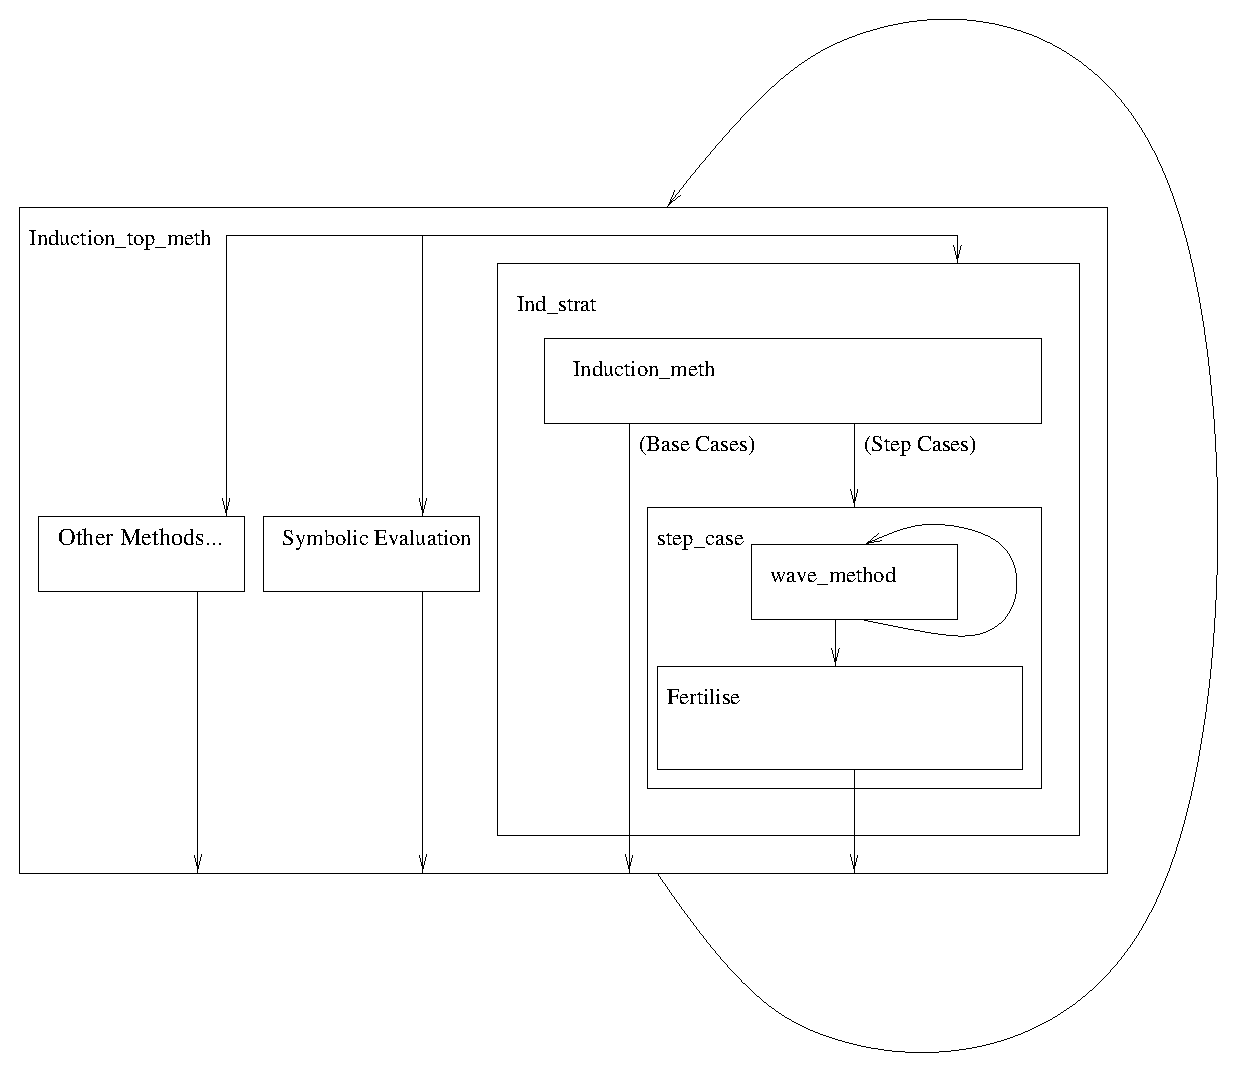
\epsfig{file=ind_strat.eps, width=4.8in}
\end{center}
\caption{The Proof Strategy for Induction}
\label{fig:induction_strategy}
\end{figure}
This is implemented as a selection of atomic and compound methods.
The diagram shows a top level repeat which attempts a disjunction of
methods.  These include basic tautology checking, generalisation of
common subterms and also symbolic
evaluation and the induction strategy ({\tt ind\_strat}).  Within the
induction strategy, the induction method
performs ripple
analysis~\cite{ind-chap-ref2} to choose an induction scheme (from a
selection specified in \lclam's theories) and produces subgoals for
base and step cases.  The base cases
are passed out to the repeat of the top level strategy.
The step cases are annotated with \emph{skeletons} and
\emph{embeddings} (described 
below) and then the wave method is repeatedly applied to them followed 
by fertilisation (exploitation of the induction hypothesis).
Annotations are then removed.  The methods ({\tt set\_up\_ripple} and
{\tt post\_ripple}) which place and remove annotations are omitted
from the diagram.  The results are then passed out to the top level
strategy again.  The process terminates when all subgoals have been
reduced to \emph{true} (or \emph{false} in the case of failure).

We will discuss the \method{wave\_method} in more detail since it was
a new formulation of this method we wished to investigate.  The wave
method embodies the rippling heuristic.  Rippling was first introduced
in~\cite{pub567}.  We use the theory as presented by Smaill \&
Green~\cite{pub799} who proposed a version that naturally coped with
higher-order features.  Rippling steps apply rewrite rules to a target
term which is associated with a skeleton and an embedding
that relates the skeleton to the target term (e.g.
rippling\index{rippling} rewrites an induction conclusion which has an
induction hypothesis embedded in it).  In the present context, we make
use of higher order rewriting, in the style of \cite{Fel92}.  After rewriting a new embedding of the skeleton into the rewritten term is calculated.  There is
a measure on embeddings and any rewriting step must reduce this
\emph{embedding measure} (written as $<_{\mu}$).  This is a
generalisation of the original version of rippling that used annotated
\emph{wave rules} to rewrite annotated terms.

Rippling is terminating~\cite{BasinWalsh96}.  Rippling either moves
differences outwards in the term structure so that they can be
cancelled away or inwards so that the differences surround a
universally quantified variable (or \emph{sink}).  If it is possible
to move differences inwards in this way the embedding is said to be
\emph{sinkable}.  The measure on embeddings allows differences that
are being moved outwards to be moved inwards but not vice versa --
this is at the heart of the guarantee of termination.

The \method{wave\_method} method has five preconditions.  It finds a
rewrite rule that rewrites the goal.  It then checks that there is
still an embedding of the skeleton into the rewritten goal and that
this new embedding is less, according to the embedding measure, than
the original embedding.  It checks that the embedding is sinkable and
that any conditions for the application rule are trivial.  This is
shown in figure~\ref{fig:wave_method}.  
%Sinkability is not necessary
%for termination but it is a useful further heuristic for guiding the
%proof.
\begin{figure}[htb]
\pageline
% \vspace{1mm}
\begin{center}
\begin{center}
\textbf{Input}

$$ripple\_goal(H \vdash G, S, E).$$
where $ripple\_goal$ is a triple of a sequent, a skeleton, $S$ and an
embedding, $E$, of that skeleton into the goal, $G$.
\end{center}
\begin{center}
\textbf{Preconditions}
\end{center}

\begin{enumerate}
\item The conditional
  rewrite rule \emph{Rule}, $Cond \imp X \rewrites Y$ instantiated
  with some substitution $\sigma$, applies to $G$
  and rewrites it to $G'$.
\item There is an embedding $E'$ that embeds $S$ in $G'$.
\item $E' <_{\mu} E$.
\item $\sigma(Cond) = True$ or $\sigma(Cond) \in H$.
\item $E'$ is sinkable.
\end{enumerate}
\begin{center}
\textbf{Output}
\end{center}
$ripple\_goal(H \vdash G', S, E')$
\end{center}
\vspace{1mm}
\pageline
\caption{The Wave Method}
\label{fig:wave_method}

\end{figure}
The method will backtrack\index{backtracking} in order to try to
satisfy all requirements, and if it is successful returns a new goal.

%The main advantages of rippling is that it allows an equation
%to be treated as a rewrite in both directions without loss of
%termination and provides useful information for automatically patching 
%failed proof attempts.  These abilities were not required in this case 
%studies and all the proofs went through automatically using 
%symbolic evaluation instead of rippling.  However, our intention was
%to test the higher-order presentation of rippling \emph{not} to justify 
%its necessity in the case of ordinals.

\section{Embeddings}
\label{embeddings}
We review here the notion of embeddings from Smaill \&
Green \cite{pub799}.  These provide the higher-order framework for
rippling used in this paper.

Embeddings are described by a tree data structure.  Embedding trees
describe how a \emph{skeleton} embeds in a term, called
the \emph{erasure}.  The nodes in an embedding tree
can be viewed as labels on the nodes in the term tree of the skeleton.
These labels contain addresses and directions.  The directions are
used during rippling as outlined above.  The addresses
are the addresses of nodes in the term tree of the erasure which
correspond to that node in the skeleton.  Term trees represent
function application and $\lambda$-abstraction explicitly as nodes with
constant and variables symbols appearing only at the leaves of the
tree.  Our implementation also contains tuple nodes for lists of
arguments to functions but these are not necessary to the theory.
Embeddings do not annotate $\lambda$-abstraction nodes.  Where an
embedding matches a variable in the skeleton to one in the erasure it
indicates that they are $\alpha$-convertible.
It is the ability to coherently handle
$\lambda$-abstractions which was particularly valuable in this
experiment.  The ability to handle difference occuring within functions as well
as the arguments to functions is also an extension of the previous
calculus.

\begin{example}
Consider embedding the term $\lam{x} f(x)$ into the term
$\lam{y} \lam{x} (f(y) + x)$. We 
do this as in figure~\ref{fig:embed}.  The two terms are shown 
as trees with branches represented by solid lines.  The address of
each node is given ($\lambda$-abstraction nodes do not carry
addresses).  The embedding appears
between them as an  
embedding tree with dashed lines -- the address label of
the nodes is 
also shown.  The dotted arrows illustrate how the embedding tree links 
the two terms.

\begin{figure}[htb]
\begin{center}
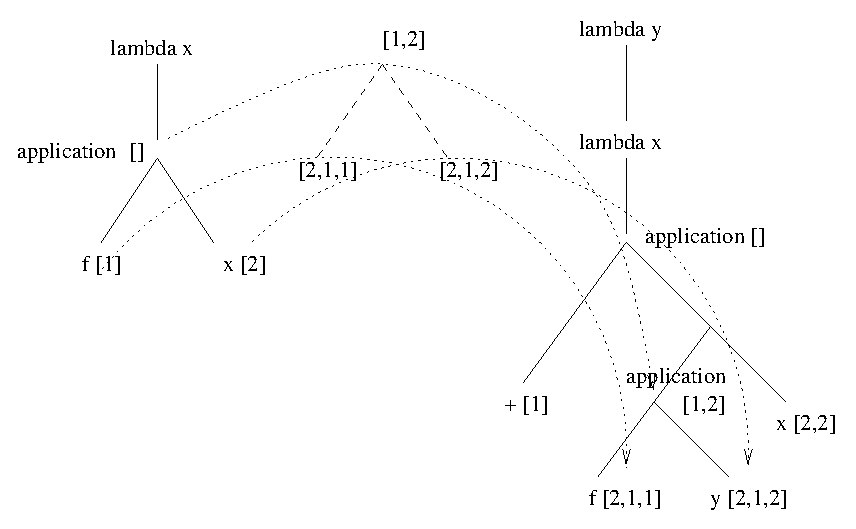
\epsfig{file=embed.eps, width=3in}
\end{center}
\caption{An Embedding}
\label{fig:embed}
\end{figure}

The embedding tree for this is  (node [1, 2] [(leaf
[1, 1, 1]) (leaf [2, 1, 2])])).  This states
that the function 
application at the top of $f(x)$ matches with the node at
address [1, 2] of $f(y) + x$ (i.e. the application involving $+$ has
been bypassed), that the
function symbol $f$ matches the sub term at [2,1,1] (i.e. $f$)
and $x$ matches $y$ (i.e.\ the bound variables can be consistently
renamed in either (or both) terms so that they are identical).

The annotations originally used in rippling 
are still useful for presentation.  Annotations consist of contexts
(expressions 
with holes) indicated by a wave front (box) with a directional arrow.
The holes in the context are wave holes (i.e. they are filled with an
expression which is underlined). The skeleton is everything
that appears outside wave fronts, or in wave holes. 
So the above embedding can be
presented as 
$$
\lam{x} \wfout{\lam{y} \wh{f(y)} + x}.
$$

NB.  It is important to remember that the annotations do not actually
exist in the implementation which records instead the 
skeleton and embedding\footnote{In fact \lclam\ maintains a list of
possible embeddings 
during rippling since there may be more than one way to embed the
induction hypotheses into the conclusion.  For convenience we assume
here there is only one.}.  
In some cases it is less easy to use the
traditional annotations to represent embeddings, particularly when dealing
with $\lambda$-abstrations which are ignored by the embedding trees.
You can see that in the above the bound variables in the skeleton 
are assumed to have been appropriately renamed already.
These 
annotations are just a presentational convenience.
\end{example}

\section{Logics}
You will note that the proof strategy for induction calls the {\tt
  taut}\index{taut} method for tautology checking.  This may vary
depending upon whether constructive or classical logic (for instance)
is being used.  As a result the basic ``build'' of the induction
theory\index{induction theory} in \lclam\ does not specify how the
{\tt taut} method or logical constants such as {\tt
  forall}\index{forall} or {\tt and}\index{and} should be treated by
the system.  It simply asserts that they exist.  Additional files, of
which the {\tt constructive\_logic}\index{constructive\_logic} theory
can then be created to provide the necessary details.

\section{Arithmetic, Natural Numbers and Lists}
There are a number of built-in theories dealing with natural number
and list theorems.  Standard functions and goals can be found in the
{\tt arithmetic}\index{arithmetic} theory and the {\tt
  objlists}\index{objlists} theory.  Further functions can be found in 
{\tt list\_benchmarks}\index{list\_benchmarks}, {\tt
  map\_benchmarks}\index{map\_benchmarks} and the {\tt
  clam\_corpus}\index{clam\_corpus} theories (there are 3 clam corpus
theory files).

\section{Mutual induction}
\noindent 
This module was written for the MFOTL group based at Liverpool.  The
method \texttt{alexei\_meth} in
\texttt{theories/mutual\_induction.mod} implements the following proof
rule.  It is a variant of a mutual induction rule suitable for
treatment of arithmetical translations of temporal formulae:

\vspace{0.5cm}

$ \forall y \forall \bar{x} A_{1}(y, \bar{x}) \Rightarrow B_{1}(s(y), \bar{x})$

$\forall y \forall \bar{x} A_{2}(y, \bar{x}) \Rightarrow B_{2}(s(y), \bar{x})$

$\ldots $

$\forall y \forall \bar{x} A_{n}(y, \bar{x}) \Rightarrow B_{n}(s(y), \bar{x})$

\vspace{-1mm}
$\underline{\qquad\qquad\qquad\qquad\qquad\qquad\qquad\qquad\qquad\qquad}$
 
\vspace{1mm}
$\forall u. u > t \Rightarrow \varphi(u)$ 

\vspace{5mm}
\noindent
with the side conditions: 

\[\begin{array}{l} 
\exists \bar{x}  (A_{1}(t,\bar{x}) \vee A_{2}(t, \bar{x}) \vee \ldots \vee 
A_{n}(t,\bar{x})) \\
\\
\forall y \forall \bar{x} (B_{i}(y, \bar{x}) \Rightarrow \varphi(y)) , i=1, \ldots, n \\
\\
\forall y \forall \bar{x} \exists \bar{z} ( B_{i}(y, \bar{x}) 
\Rightarrow \bigvee_{j=1\ldots n} A_{j}(y,\bar{z})) ,  i=1 \ldots, n 
\end{array}\]

\noindent
where $A_{i}$ and $B_{i}$ are arbitrary first-order formulae, $t$ is
an arbitrary arithmetical term, s is the successor function symbol,
$\Rightarrow$ is implication, $\bar{x}$ is a sequence of
variables, and $y$ is a (numerical) variable of type \texttt{nat}.  $n$ is
not fixed, so we can deal with arbitrary lists of premises in the rule.

\noindent
Since the rule is generally used in backward reasoning, 
one can present its application as follows: \\

\noindent
Given a goal sequent $H \vdash \psi$ with $\psi$ being of the form of
the conclusion of the above rule, the method generates some subset
$H'$ of $H$ matching the premises of the rule and generates the
associated side conditions as new subgoals.  These subgoals are
then resolved by application of some other methods (for first-order
reasoning). \\

\noindent
At present the method simply chooses the maximal matching subset of
hypotheses.  Probably some optimization for iteration over subsets
will be needed later.

\noindent{\bf Example:} \\

Given:   
\[\begin{array}{l}
\forall x, y (A(y,x) \Rightarrow B(s(y),x)) \\
\forall x, y (C(y,x) \Rightarrow D(s(y),x)) \\
\forall x (A(0,x) \lor C(0,x)) \\
\forall x,y (B(y,x) \Rightarrow C(y,x)) \\
\forall x,y (D(y,x) \Rightarrow (A(y,x) \lor C(y,x))) 
\end{array}\]

\vspace{-1mm}
$\underline{\qquad\qquad\qquad\qquad\qquad\qquad\qquad\qquad\qquad\qquad\qquad}$

Prove: 
\[\forall y > 0  \exists x (B(y,x) \lor D(y,x)) \]
 
Side conditions to prove (taking the set of first two hypotheses and the
conclusion):

\[\begin{array}{l}
\exists x (A(0,x) \lor C(0,x))\\
\\
\forall y \forall x (B(y,x) \Rightarrow  \exists z (B(y,z) \lor D(y,z))) \\
\\
\forall y \forall x (D(y,x) \Rightarrow  \exists z (B(y,z) \lor D(y,z))) \\
\\
\forall y \forall x \exists z (B(y,x) \Rightarrow A(y,z) \lor C(y,z)) \\
\\
\forall y \forall x \exists z (D(y,x) \Rightarrow A(y,z) \lor C(y,z)) \\
\end{array}\]
\newcommand{\lyacc}{$\lambda$yacc\xspace}

\chapter{Compiling Theories to \lclam}\label{compiler}

%\author{Ewen Denney}

\section{Introduction}

This chapter describes the current state of the \lclam theory
compiler.  It develops the idea that a logic can be presented in a
high-level declarative style, and then {\em compiled} down into a more
procedural implementation-specific language.

The reasons for wanting to do this are:
\begin{itemize}
\item the user-unfriendliness of the current \lclam format
\item to avoid errors that can arise when entering axioms and
  inferences as low-level rewrites and methods
\item (ultimately) to aim for a logic-independent planner by factoring out
  logic-specific code
\item since a high-level representation of logics and theories, rather than
  one which is hard-wired into a low-level implementation, is easier
  to communicate.
\end{itemize}

In our case, of course, the procedural language is \lclam's format for
the paraphernalia of proof planning (expressed in HOAS) in \lprolog;
for declarative language, we simply make up our own user-friendly
syntax for declarations, inference rules, and the like.


The compiler has two modes of use: online, using the {\tt add\_theory}
command during \lclam's normal command loop, and offline, generating a
separate \lclam theory file.  The offline mode is currently deprecated
but is described here as it helps understand the general compilation
process and may prove useful in the future.

\section{Online Mode}

The command
$${\tt add\_theory} \mbox{\em ``theory-file''}$$
will read in the file
{\em theory-file}, check its well-formedness, and generate the
appropriate user-defined constants.

For example, the file {\tt simpletheory}:
\begin{verbatim}
Theory Nsa.
Use Logic arithmetic.

type real.
type hyperreal.
$
\end{verbatim}
gives the following results:
\begin{verbatim}
lclam:
add_theory "simpletheory".
Trying ...Scanning for tokens...
Tokenizer stopped after line 6
Parsing...
Successfully parsed
Checking well-formedness...
Type real
Type hyperreal
Theory is well-formed
Importing lclam declarations...
Successfully processed
Done
Done
lclam:
\end{verbatim}
We can now use the query commands to check that the definitions have been made
correctly.
\begin{verbatim}
lclam:
query_osyn (user_theory "nsa") (user_object "real") X.
default
user_theory "nsa"
real
universe
lclam:
\end{verbatim}

A more complex example of a theory file can be seen in
Section~\ref{theory}.

\section{Offline Mode}

We describe here how a user can use the files {\tt
  envgrammar.\{sig,mod\}} and\linebreak 
{\tt postprocess.\{sig,mod\}} in the
{\tt compiler} directory to parse a theory file written in concrete
syntax and generate a \lclam theory file.

We first explain how to use the compiler, and in the following
sections, explain the workings of the compiler in case the user wants
to alter it.

The phases of such a logical compilation are much the same as in the
compilation of programs: parsing of concrete into abstract syntax
(Section \ref{parsing}), a well-formedness check (Section
\ref{well-formedness}), and then code generation (Section
\ref{generation}). We give the grammar for theory files (Section
\ref{grammar}), and examples of concrete syntax (Section \ref{theory}) and
the corresponding \lclam (Section \ref{lclam}).


\subsubsection{Using the Compiler}\label{makefile}

First, edit the {\tt Makefile}, if necessary, to alter the paths appropriately.

Then, generate the parser by
\begin{alltt}
make envparser
\end{alltt}
Next, do
\begin{alltt}
make postprocess
\end{alltt}

If the theory file is {\tt theoryfile}, then the command
\begin{alltt}
parsefile "theoryfile" X.
\end{alltt}
will bind to $\tt X$ the abstract syntax that results from parsing
this file. This might be useful to you if you just want access to the
higher-order abstract syntax form of an expression.

Here, {\tt theoryfile} is the file with concrete syntax which you can,
of course, change and rename. Note that the underlying parser, \lyacc,
requires this file to terminate with a {\tt \$}.

The command
\begin{alltt}
process_file "theoryfile"
\end{alltt}
will parse the file, check its well-formedness, and output the
appropriate \lclam files. The names of the files are determined by
the line
\begin{alltt}
Theory <name>.
\end{alltt}
in the theory file, which results in {\tt <name>theory.\{sig,mod\}}. 

Finally, you then have to fit these files in with your version of
lambda clam (by setting the appropriate accumulates) and compile the
whole system. Note that the compilation files themselves should not be
compiled with \lclam.


\subsection{Parsing}\label{parsing}

The logic file is first parsed into abstract syntax. The parser is
implemented using 
\lyacc\footnote{See {\tt http://www.cs.hofstra.edu/\~{ }cscccl/parsergen/.}}, 
a parser-generator written in \lprolog, due to Chuck Liang. It
generates bottom-up {\em shift-reduce} parsers, which can be less
intuitive than top-down parsers, but are more efficient.

The user specifies their logic by writing various predicates and rules
in a \lprolog file, which accumulates the \lyacc files.

\begin{enumerate}
\item Declare grammar symbols for the abstract syntax for each nonterminal.
\item Declare the terminals.
\item Give concrete syntax for the terminals using {\tt printname}.
\item List the terminals, and nonterminals.
\item Set {\tt ntnum} to the number of nonterminals plus 1.
\item
Give the parse rules, with semantic actions to construct
the abstract syntax.

For example, rules giving the syntax for axiom declarations are
\begin{verbatim}
 rule ((syn_decl_gs D5) ==> 
        [axiom_decl_gs S7 H1 Z7]) (D5 = axiom_decl S7 H1 Z7),

 rule ((axiom_decl_gs S5 H2 Z5) ==> 
        [axiomt, axiom_name I6, qprop_gs Z3, periodt]) 
                                (S5 = I6, Z5 = Z3, H2 = []),
\end{verbatim}
The {\tt rule} construct combines a production with a semantic action.
\item
Give precedence rules.
\item Supply freshcopy clauses for non-nullary nonterminals.
\end{enumerate}


This file is compiled, and then executed. Then, a generate parser
command is called, which, assuming \lyacc accepts the file, generates
{\em another} file. This file is then compiled to give the parser, all
of which takes about a minute in total.


\subsection{Well-formedness}\label{well-formedness}

A consequence of the fact that the semantic actions attached to \lyacc
parse rules cannot contain implications (and that \lprolog does not
have assertions), is that well-formedness of the resulting abstract
syntax has to be checked in a separate pass.

However, logically inspired manipulation of terms such as this is what
\lprolog does best.  For example, well-formedness of existentials and
abstractions is checked by
\begin{verbatim}
well_formed_assertion (app exists (tuple [T, abs P])) :-
        well_formed_type T,
        pi X \ (new_const X T) => well_formed_assertion (P (user_object X)). 

well_typed_term (ty_abs T L) (T arrow U) :-
        well_formed_type T,
        pi X \ (new_const X T) => well_typed_term (L (user_object X)) U.
\end{verbatim}
Since declarations are `first-class' in \lprolog, \lprolog's context
mechanism can be used for managing declarations.

\begin{verbatim}
well_formed_decls ((inference_decl S Hyps H2 C2)::Ds) :-
        well_formed_decl (inference_decl S Hyps H2 C2),
        ((new_inference S) => well_formed_decls Ds).

well_formed_decl (inference_decl S Hyps H2 C2) :-
        not (new_inference S),
        map_pred2 group_assertions Hyps Ass,
        all_pred well_formed_assertions Ass,
        ly_append H2 [C2] Ps2,
        well_formed_assertions Ps2,
        M is "Inference " ^ S ^ "\n",
        print M.
\end{verbatim}
There are no error messages at present.

\subsection{Generation of \lclam}\label{generation}
Once the theory file has been parsed into abstract syntax and checked
for well-formedness, it is converted to \lclam format and written to a
file. Constructing the appropriate higher-order abstract syntax was
done during parsing, so this stage is mainly concerned with
abstracting over the variables, and converting propositions to
rewrites and methods.

The syntax comprises a list of declarations, each of which is
converted to the corresponding \lclam entity.

\begin{alltt}
% decl2lclam {\it +sig-file +mod-file +theory-name +logic-name +declaration}

type decl2lclam  out_stream -> out_stream -> string -> string -> syn_decl -> o.
\end{alltt}
A syntactic declaration is one of: type, typed constant, axiom,
inference, conjecture, predicate symbol, definition.  The interesting
cases are axiom and inference rules. We convert axioms to rewrite
rules, and inferences to methods.

An example of an axiom is
\begin{verbatim}
axiom ax1 [y:nat |- forall f:nat->nat. f = (x:nat \ (f y))].
\end{verbatim}
This is parsed as
\begin{verbatim}
axiom_decl "ax1" (otype_of (user_object "y") nat :: nil) 
   (app forall (tuple ((nat arrow nat) :: 
         abs (W1\ app eq 
          (tuple (W1 :: ty_abs nat (W2\ app W1 (user_object "y")) :: nil))) ::
 nil)))
\end{verbatim}
and converted to the rewrite rule
\begin{verbatim}
axiom nsa ax11 ltor (trueP) 
   (app forall 
     (tuple ((nat arrow nat) :: 
       abs (W1\ app eq (tuple (W1 :: ty_abs nat (W2\ app W1 _107597) :: nil)))
 :: nil))) 
    (trueP).
\end{verbatim}


For inference rules, the system generates preconditions to check
for required antecedents in the conclusion, and to construct the
antecedents of the hypotheses. The succedent of the conclusion is
recorded in the form of the method input, and the succedents of the
hypotheses appear in the output goal.

For example, the inference rule
\begin{verbatim}
inference and_l [G,A,B,G' |- P / G, A /\B |- P]
\end{verbatim}
parses to abstract syntax
\begin{verbatim}
(inference_decl "and_l"
[(pair [user_object "G", user_object "A", user_object "B", user_object "G'"] 
       (user_object "P"))]
[user_object "G", (app and (tuple [user_object "A", user_object "B"])), 
user_object "G'"] (user_object "P"))
\end{verbatim}
which is converted to the atomic method
\begin{verbatim}
atomic nsa and_l
        (seqGoal (H >>> (_9055)))
        (sublist (app and (tuple (_9072 :: _9088 :: nil)) :: nil) H, 
        replace_in_hyps H (app and (tuple (_9072 :: _9088 :: nil))) 
                             (_9072 :: _9088 :: nil) H1)
        true
        seqGoal (H1 >>> _9055)
        notacticyet.
\end{verbatim}
The inference rule
\begin{verbatim}
inference and_r [G |- A ; G |- B / G |- A /\B]
\end{verbatim}
parses to abstract syntax
\begin{verbatim}
(inference_decl "and_r"
[(pair [user_object "G"] (user_object "A")),
(pair [user_object "G"] (user_object "B"))]
[user_object "G"] (app and (tuple [(user_object "A"), (user_object "B")]))
)
\end{verbatim}
and converts to
\begin{verbatim}
atomic nsa and_r
        (seqGoal (H >>> (app and (tuple (_5035 :: _5052 :: nil)))))
        (H =  H1, H =  H2)
        true
        seqGoal (H1 >>> _5035) ** seqGoal (H2 >>> _5052)
        notacticyet.
\end{verbatim}


\subsection{Theory Grammar}\label{grammar}

Identifiers can contain underscores but not hyphens. A theory begins
with a declaration of its name, and the logic it uses. The logic name
is not used, but must be entered for syntactic correctness.

\begin{verbatim}
Theory-declaration ::= 
        'Theory' Id '.'
        'Use Logic' Id '.'
        (Declaration '.')*

Declaration ::= Constant-declaration
                | Type-declaration
                | Axiom-declaration
                | Inference-declaration
                | Conjecture-declaration
                | Predicate-declaration
                | Definition


Constant-declaration ::= 'const' Id Type

Type-declaration ::= 'type' Id

Axiom-declaration ::= 'axiom' Id Prop | 'axiom' Id '[' Sequent ']' 

Inference-declaration ::= 'inference' Id '[' Sequents '/' Sequent ']'

Conjecture-declaration ::= 'conjecture' Id '[' Sequent ']'

Predicate-declaration ::= 'predicate' Id Type+

Definition ::= 'define' 'const' Id ':' Type '=' Term
             | 'define' 'type' Id '=' Type

Sequents ::= (Sequent ';')* Sequent

Sequent ::= Assumptions '|-' Prop

Assumptions ::= (Assumption ',')* Assumption

Assumption ::= Prop | Id ':' Type

Prop ::= 'forall' Id ':' Type '.' Prop
       | 'exists' Id ':' Type '.' Prop
       | Prop '/\' Prop
       | Prop '\/' Prop
       | Prop '=>' Prop
       | '<' Term '=' Term '>'
       | '(' Prop ')'
       | Id
       | Id '{' Term '}'

Type ::= nat | bool | '(' Type ')' | Type '->' Type | Type '#' Type | Id

Term ::= Id
       | (Id ':' type '\' Term ')'
       | '<' Term Term '>'
\end{verbatim}

\subsection{Theory file}\label{theory}
\begin{verbatim}
Theory Nsa.
Use Logic Thol.

type real.
type hyperreal.
const z nat.
const f nat->nat#bool.

axiom sch2 [x:nat |- <x=x>].
axiom sch3 [x:nat, y:nat |- <x=y>].
axiom sch4 [x:nat, y:nat, <x=y> |- <y=x>].
axiom ax1 [y:nat |- forall f:nat->nat. <f = (x:nat \ <f y>)>].
axiom exax exists x:nat. <x=x>.
axiom badax [true, x:nat |- <x=x>].

conjecture conj1 [x:nat |- forall y:nat . <x=y>].
inference inf1 [true |- false / true, x:nat |- <x=x>].

axiom qs (forall x:nat. (exists y:nat. <x=y>)) => true.

conjecture conj2 [x:hyperreal |- exists y:hyperreal . <x=y>].

predicate even : nat.
predicate close_to : hyperreal, real.

inference easy_inf [true|-true; false|-false / x:nat |- <x=x>].

axiom pred_in_prop even{z}.

define type real_pair = real#real.

define const n:nat#bool = <f z>.

define const m:nat = z.

axiom false_e [G1, false, G2 |- P].

inference and_r [G |- A; G |- B / G |- A /\ B].

inference and_l [G1,A,B,G2 |- P / G1, A /\B,G2 |- P].

inference or_l [G,A |- P; G,B |- P / G, A\/B |- P].
\end{verbatim}

\subsection{Generated \lclam}\label{lclam}
\begin{verbatim}
module nsatheory.

all_pred P nil.
all_pred P (H::T) :- P H, all_pred P T.
sublist Xs Ys :- all_pred (X\ (member X Ys)) Xs.

has_otype nsa real universe.
has_otype nsa hyperreal universe.
has_otype nsa z (nat).
has_otype nsa f (nat arrow tuple_type (nat :: bool :: nil)).
axiom nsa sch21 ltor (trueP) (_135695) (_135695).

axiom nsa sch22 ltor (trueP) (app eq (tuple (_137129 :: _137129 :: nil))) 
(trueP).

axiom nsa sch31 ltor (trueP) (_137732) (_137749).

axiom nsa sch41 ltor (app eq (tuple (_139400 :: _139383 :: nil))) (_139383) 
(_139400).

axiom nsa sch42 ltor (app eq (tuple (_144856 :: _144839 :: nil))) (app eq 
(tuple (_144839 :: _144856 :: nil))) (trueP).

axiom nsa ax11 ltor (trueP) (app forall (tuple ((nat arrow nat) :: abs (W1\ 
app eq (tuple (W1 :: ty_abs nat (W2\ app W1 _147505) :: nil))) :: nil))) 
(trueP).

axiom nsa exax1 ltor (trueP) (app exists (tuple (nat :: abs (W1\ app eq (tuple
 (W1 :: W1 :: nil))) :: nil))) (trueP).

axiom nsa badax1 ltor (trueP) (_148474) (_148474).

axiom nsa badax2 ltor (trueP) (app eq (tuple (_149926 :: _149926 :: nil))) 
(trueP).

top_goal nsa conj1 [(otype_of (user_object "x") nat)] (app forall (tuple (nat 
:: abs (W1\ app eq (tuple (user_object "x" :: W1 :: nil))) :: nil))).
atomic nsa inf1
        (seqGoal (H >>> (app eq (tuple (_152632 :: _152632 :: nil)))))
        (sublist (trueP :: otype_of (user_object "x") nat :: nil) H)
        true
        (seqGoal (H1 >>> falseP))
        notacticyet.

axiom nsa qs1 ltor (trueP) (trueP) (app forall (tuple (nat :: abs (W1\ app 
exists (tuple (nat :: abs (W2\ app eq (tuple (W1 :: W2 :: nil))) :: nil))) :: 
nil))).

axiom nsa qs2 ltor (trueP) (app imp (tuple (app forall (tuple (nat :: abs (W1\
 app exists (tuple (nat :: abs (W2\ app eq (tuple (W1 :: W2 :: nil))) :: 
nil))) :: nil)) :: trueP :: nil))) (trueP).

top_goal nsa conj2 [(otype_of (user_object "x") (user_object "hyperreal"))] 
(app exists (tuple (user_object "hyperreal" :: abs (W1\ app eq (tuple 
(user_object "x" :: W1 :: nil))) :: nil))).
atomic nsa easy_inf
        (seqGoal (H >>> (app eq (tuple (_156487 :: _156487 :: nil)))))
        (sublist (otype_of (user_object "x") nat :: nil) H, replace_in_hyps H 
(otype_of (user_object "x") nat) (falseP :: nil) H1, replace_in_hyps H 
(otype_of (user_object "x") nat) (trueP :: nil) H2)
        true
        (seqGoal (H1 >>> trueP) ** seqGoal (H2 >>> falseP))
        notacticyet.

axiom nsa pred_in_prop1 ltor (trueP) (app (user_object "even") (user_object 
"z")) (trueP).

definition nsa real_pair0 trueP (tuple_type (user_object "real" :: user_object
 "real" :: nil)) real_pair.
definition nsa n0 trueP (app (user_object "f") (user_object "z")) n.
definition nsa m0 trueP (user_object "z") m.
atomic nsa false_e
        (seqGoal (H >>> (_25170637)))
        (sublist (falseP :: nil) H)
        true
        trueGoal
        notacticyet.

atomic nsa and_r
        (seqGoal (H >>> (app and (tuple (_162845 :: _162862 :: nil)))))
        (true, H =  H1, H =  H2)
        true
        (seqGoal (H1 >>> _162845) ** seqGoal (H2 >>> _162862))
        notacticyet.

atomic nsa and_l
        (seqGoal (H >>> (_186518)))
        (sublist (app and (tuple (_186535 :: _186551 :: nil)) :: nil) H, 
replace_in_hyps H (app and (tuple (_186535 :: _186551 :: nil))) (_186567 :: 
_186535 :: _186551 :: _186583 :: nil) H1)
        true
        (seqGoal (H1 >>> _186518))
        notacticyet.

atomic nsa or_l
        (seqGoal (H >>> (_197214)))
        (sublist (app or (tuple (_197231 :: _197247 :: nil)) :: nil) H, 
replace_in_hyps H (app or (tuple (_197231 :: _197247 :: nil))) (_197247 :: 
nil) H1, replace_in_hyps H (app or (tuple (_197231 :: _197247 :: nil))) 
(_197231 :: nil) H2)
        true
        (seqGoal (H1 >>> _197214) ** seqGoal (H2 >>> _197214))
        notacticyet.

end

\end{verbatim}



%=========================
%%   Systemnamen
%%=========================

\newcommand{\Nat}{{\mathchoice{\displaystyle\rm I\hskip-0.21em N}%
{\textstyle\rm I\hskip-0.21em N}%
{\scriptstyle\rm I\hskip-0.14em N}%
{\scriptscriptstyle\rm I\hskip-0.14em N}}}
%%%%%%%%%%%%%%%%%%%%%%%%%%

\def\eps{\epsilon}
\def\name#1{#1}
\def\xspace{}
\def\activemath{{\it ActiveMath}}
\def\analytica{{\it Analytica}}
\def\automath{AUTOMATH}
\def\bliksem{{\it Bliksem}}
\def\chip{\mbox{CHIP}\xspace}
\def\chorus{Chorus}
\def\clamlite{{CLAM-Lite}}
\def\clos{{{\small CLOS}}}
\def\commonlisp{{{\footnotesize COMMON LISP}}}
\def\corba{{\sc Corba}}
\def\cosie{${\cal C}o{\cal SIE}$}

\def\davinci{\mbox{\sc daVinci}\xspace}
\def\declame{{{\small DECLAME}}}
\def\discount{{DISCOUNT}}
\def\doris{DORIS}
\def\eclipse{ECL$^i$PS$^e$}
\def\eqp{EQP}
\def\eprover{{\sf E}}

\def\fipa{{\sf FIPA}}
\def\fscos{${\cal FSC}o{\cal S}$}
\def\HOL{{$\cal HOL$}}
\def\hr{{\sf HR}}
\def\http{{\sf http}}

\def\ilf{{ILF}}
\def\ilog{ILOG}
\def\imply{IMPLY}
\def\imps{\mbox{\sc IMPS}\xspace}
\def\isabelle{\mbox{\it Isabelle}\xspace}

\def\keim{{\small\bf KEIM}}
\def\KEIM{{\small\bf KEIM}}
\def\kimba{{\sf Kimba}}
%\def\kqml{{\sc Kqml}}
\def\kqml{KQML}
\def\larks{LARKS}
\def\mathml{{\sc MathML}}
\def\oants{{\sf OANTS}}
\def\omrs{{\sc OMRS}}
\def\openmath{{\sc OpenMath}}
\def\omdoc{{OMDoc}} %\protect\omdocaux}
\def\omdocaux{\sc O\kern-1.6ex\raisebox{.4ex}{{\tiny M}}Doc}
\def\prosper{{\sc Prosper}}
\def\pvs{PVS}
\def\setheo{{SETHEO}}
\def\teamwork{{\sc Teamwork}}
\def\techs{{TECHS}}
\def\waldmeister{Waldmeister}
\def\xml{XML}
\def\xsl{{\sc Xsl}}

\def\lams{{\sf LaMS}}
\def\leo{\mbox{${\cal LEO}$}\xspace}
\def\lineq{{\sc LinEQ}}
\def\lisp{{\footnotesize LISP}}
%\def\loui{\mbox{{\sc L}$\Omega${\sc UI}}\xspace}
\def\LOUI{\mbox{\sc L}{\sc ovely} {$\Omega${\sc mega}} {\sc U}{\sc ser} {\sc I}{\sc nterface}}

\def\gap{GAP}
\def\cocoa{CoCoA}
\def\lba{LBA}
\def\lclam{\mbox{$\lambda$\--Clam}}
\def\mace{MACE}
\def\magma{{\sc MagMa}}
\def\maple{{\sc Maple}}
\def\mass{{\sc Mass}}
\def\mathematica{{\it Mathematica}}
\def\mathpert{{\it Mathpert}}
\def\mathweb{Math\-Web}
\def\mathwebsb{Math\-Web-SB}
\def\mathagent{\mbox{\sc MathAgent}\xspace}
\def\mbase{{\sc MBase}}
\def\mkrp{{MKRP}}
\def\mosh{\sc MoSh}
\def\mozart{\sc Mozart}
\def\multi{MULTI}
\def\mycas{\mbox{$\mu$\hspace{.2em}${\cal CAS}$}}
\def\MYCAS{\mbox{$\mu${\sc CAS}}}
\def\myCAS{\mbox{$\mu${\sc CAS}}}

\def\ND{{\small\bf ND}}
\def\nuprl{{Nuprl}}
\def\octopus{\mbox{$\Omega${\sc cTOpus}}\xspace}
\def\OMEGA{$\Omega${\sc mega}}
\def\omws{OMWS}
\def\otter{{\sc Otter}}
\def\oyster{{\mbox{\rm O\kern-.12em\raise.39ex\hbox{\sc y}\kern-.07emS\kern-.39em\raise.39ex\hbox{\sc t}\kern-.15em\hbox{\sc e}R}}}
\def\oz{{\sc Oz}}

\def\pds{PDS}
\def\POST{{\mbox{$\cal POST$}}}
\def\post{{\POST}}
\def\Post{{\POST}}
\def\prolog{PROLOG}
\def\lprolog{$\lambda$-PROLOG}
\def\protein{\mbox{\sc ProTeIn}\xspace}
\def\proverb{{\it PROVERB\/}}
\def\rdl{{\bf RDL}}
\def\sapper{{\sc sapper}}
\def\scetchpad{\mbox{SCETCHPAD}}
\def\solex{{\bf\sf SoleX}}
\def\spass{\mbox{\sc Spass}\xspace}
\def\strips{{\small STRIPS}}
\def\teyjus{Teyjus}
\def\tramp{{\sc TRAMP}}
\def\tps{TPS}
\def\tptp{{\sc TPTP}}
\def\tptptox{tptp2X}
\def\vampire{Vampire}
\def\weierstrass{{\it Weierstrass}}
\def\xmlrpc{XML-RPC}

%%\def\CLOS{{{\footnotesize COMMON LISP Object System}}}
\def\Omegapackage{{{\small\bf OMEGA}}}
%\def\clam{{\mbox{\rm CL\kern-.36em\raise.39ex\hbox{\sc a}\kern-.15emM}}}


\def\nd{{\bf ND}-Kalk"ul}
\def\lamcalc{\mbox{$\lambda$-Kalk"ul}}
\def\todo#1{{\sc #1}}
                                %\def\proverb{\mbox{\sc Proverb}\xspace}
                                %\def\clam{\mbox{\sc Clam}\xspace}
\def\hol{\mbox{\sc HOL}\xspace}
\def\nqthm{${\sc Nqthm}$}
                                %\def\tps{\mbox{\sc Tps}\xspace}
\def\clpr{\mbox{CLP(${\cal R}$)}\xspace}
\def\lmlb{\mbox{\sc LMLB}\xspace}
\def\LMLB{\mbox{\loui} {\sc M{\sc arkup}} {\sc L}{\sc anguage} {\sc B}{\sc rowser}}
\def\lml{\mbox{\sc LML}\xspace}
\def\LML{\mbox{\loui} {\sc M}{\sc arkup} {\sc L}{\sc anguage}}

\def\calculemus{\mbox{{\sc Calculemus}}}
\def\limplus{{\sc Lim-Plus}}
\def\limtimes{{\sc Lim-Times}}


\chapter{{\lclam} in the MathWeb Software Bus}\label{mathweb}

\author{J{\"u}rgen Zimmer}\footnote{The author was supported by the
  CALCULEMUS European Union IHP grant HPRN-CT-2000-00102.} (e-mail:
{\tt jzimmer@mathweb.org})\\
{\it This chapter summarises the work done by J{\"u}rgen Zimmer
  visiting the DREAM group as a CALCULEMUS Young Visiting Researcher
  (Oct. 2001 - Mar. 2002).}


\section{Introduction}
\label{sec:mw-intro}
The MathWeb Software Bus~\cite{FraKoh:mabdl99} is a platform for
distributed automated reasoning that supports the connection of a wide
range of mathematical services by a common software
bus.\footnote{Further information about the {\mathwebsb} is available
  at \url{http://www.mathweb.org/mathweb/}.}  The {\mathwebsb}
provides the functionality to turn existing reasoning systems into
mathematical services that are homogeneously integrated into a
networked proof development environment.  Client applications can
access 23 reasoning systems, for instance, the CASs {\maple},
{\magma}, and {\cocoa}, the constraint solver {\cosie}, mediators,
model generators, such as Mace and Satchmo, and the automated theory
formation system HR.  Moreover, the {\mathwebsb} integrates nine first
order ATPs, such as Otter, Spass and Bliksem, and E.
\begin{figure}[t]
 \begin{center}
   \epsfig{figure=mathweb-arch.eps,width=9cm}
   \caption{The MathWeb Software Bus}
   \label{fig:mathweb-arch}
 \end{center}
\end{figure}

The architecture of the MathWeb system is depicted in Fig.
\ref{fig:mathweb-arch}. Local {\em brokers} provide routing and
authentication information to the mathematical services. {\mathwebsb}
wrappers encapsulate the actual reasoning systems and offer the
mathematical services to their local broker.  Client applications such
as the {\OMEGA} system, HR, or {\lclam}, connect to a MathWeb broker
and request services.  In case the requested service is found, the
client application receives a reference to a newly created {\it
  service object}. The client can then send messages directly to this
service object.

\section{Integration of {\lclam}}
\label{sec:mw-integration}
We integrated {\lclam} into the {\mathwebsb} using the methodology
that has been successfully used for the integration of other systems
like the {\OMEGA} proof planner or the higher order theorem prover
{\tps}: A {\mathwebsb} {\it wrapper} implements the interface to the
services offered by {\lclam} and has full control over {\lclam} by
simulating user input using socket communication\footnote{Note: In the
  current implementation of Teyjus, socket communication only works on
  Solaris/SunOS machines.}. {\lclam} itself can use the wrapper to
access other services as external reasoning systems.

The implementation of {\lclam}, Teyjus {\lprolog}, does not allow
programming with multiple threads. Therefore, we had to define a new
interaction mode for {\lclam} in which the system reads commands from
the {\mathwebsb} socket:
\begin{description}
\item[{\tt sock\_read\_write}:] The top-level loop of a {\lclam}
  process in {\tt sock\_read\_write} mode exclusively reads commands
  from the {\tt lclam\_server\_socket}. The user cannot interact with
  the system via the usual toplevel loop.
%\item[{\tt sock\_interactive}:] I {\lclam} is running in {\tt
%    sock\_interactive} mode, the server socket is inactive. The {\tt
%    lclam\_client\_socket} can still be used to access external
%  reasoning systems in the {\mathwebsb}.
\end{description}

\subsection{Starting {\lclam} in the {\mathwebsb}}
To use {\lclam} within the {\mathwebsb} the system has to be
started by the {\lclam} {\mathweb} wrapper which establishes a socket
connection to the Teyjus process. This means, a {\mathwebsb}
installation is required.  At the moment, installing and configuring
the {\mathwebsb} is still a bit tricky. A detailed description of how
to install and configure the {\mathwebsb} can be found on the system's
homepage \url{http://www.mathweb.org/mathweb}. In the following we
only sketch the necessary steps to get an example session running on
DREAM machines:\\

\noindent Add the {\mozart} directory of the user {\tt jzimmer} to your path:
%\begin{itemize}
%\item {\tt cd \url{~}}
%\item {\tt ln -s /hame/jzimmer/.oz}
%\end{itemize}
%Expand your path to the Mozart directory:
\begin{itemize}
\item {\tt export  PATH=\$\{PATH\}:/hame/jzimmer/.oz/bin}
\end{itemize}
You can put this line in your \url{~/.bashrc} or your \url{~/.benv} file for the sake of convenience.

\noindent Copy {\mathwebsb}'s configuration files for the DREAM environment:
\begin{itemize}
\item {\tt cd \url{~}}
\item {\tt mkdir .mathweb}
\item {\tt cp -bi /hame/jzimmer/.mathweb/*config* .mathweb/}
\end{itemize}

The {\mathwebsb} expects that the environment variable
\url{LCLAM_HOME} is set to some installation of {\lclam} (Version 3.2.
or higher). If you don't have {\lclam} installed, please set the
variable to the installation of some other user, for instance, {\tt
  export LCLAM\_HOME=/hame/jzimmer/lclam}.  The same holds for the
variables {\tt TEYJUS\_HOME} which should point to the implementation
language {\teyjus}, and {\tt TJPATH} which defines the load-path of
{\teyjus} (cf.  section \ref{install}).
% instance:
%\begin{itemize}
%\item {\tt export TEYJUS\_HOME=/net/methven/disk/reason2/src/teyjus-test/juergen/teyjus-1.0-b30p2}
%\end{itemize}


\noindent Start the {\mathwebsb} and the {\lclam} system\footnote{Note that to be able to start
  {\tt lclam-mathweb} properly you should be a member of the user
  group {\tt dreamer}. Ask \url{gordon@dai.ed.ac.uk} for details.}  :
% {\mosh}\footnote{Further
%  information about the Mozart Shell (MoSh) can be found at
%  \url{http://www.mathweb.org/mathweb/mosh/}.} on methven or the host {\tt hostname}:
\begin{itemize}
\item {\tt lclam-mathweb}
\end{itemize}
An emacs window should appear with a {\lclam} process running in {\tt
  command\_pretty} mode. The system should behave like af ``normal''
{\lclam} except that the socket connection to the {\mathwebsb} wrapper
is established before the user is allowed to type in commands.  You
can try to plan a problem which uses the simplification of the
Computer Algebra System {\maple} during the planning process by typing
in the following commands:
\begin{alltt}
   add_theory_defs_to_sym_eval_list analytica.
   set_wave_rule_to_sym_eval.
   add_to_induction_scheme_list twostep2.
   pds_plan (induction_top normal_ind) fib_goal.
\end{alltt}
You should leave your {\lclam} system by typing {\tt halt.} in the
{\lclam} prompt and then {\tt C-x C-c} in the emacs window.


%Test {\lclam} with:
%\begin{itemize}
%\item {\tt testclam}
%\end{itemize}
%An emacs window should appear with a {\lclam} process running in {\tt
%  sock\_read\_write} mode.  After {\lclam} has finshed its search for
%a proof plan or after the time limit given by the test client is
%exceeded, the service is left again and the window should disappear.
%If the test worked fine, {\lclam} should be able to use all {\mathweb}
%services.

%To start an interactive {\lclam} session with an emacs interface, go
%to your {\mosh} and type
%\begin{itemize}
%\item {\tt lclam-mw}
%\end{itemize}
%The system should behave like af ``normal'' {\lclam} except that the
%socket connection to the {\mathwebsb} wrapper is established before
%the user is allowed to type in commands.


\section{{\lclam} using {\mathweb} Services}
\label{sec:mw-using-services}
For the use of external reasoning systems, we extended {\lclam} by the
modules \url{src/io/sockets.mod} and \url{src/plan/mathweb.mod} which
abstract from socket communication details and offers a convenient
interface to the {\mathwebsb} wrapper. The main predicates of the {\tt
  mathweb} module are the following:
\begin{description}
\item[{\tt mathweb\_get\_service}:]\ \\
  \hspace*{-1cm} {\small \tt string $\rightarrow$ string $\rightarrow$ o.}\\
  takes the service name as first argument (e.g.  "MAPLE", "OTTER")
  and returns a string uniquely identifying the service object in the
  second argument, if the service is available. If the service is not
  available, the predicate returns the string {\tt "error"}.
  
\item[{\tt mathweb\_apply}:]\ \\
  \hspace*{-1cm} {\small \tt string $\rightarrow$ string $\rightarrow$
    (list (list string)) $\rightarrow$ int $\rightarrow$ (list (list
    string)) $\rightarrow$ o.}\ \\ applies a method to a service
  object identified by the first argument. The second argument is the
  name of the service method. The third argument is a list of lists of
  strings representing the parameters for the method call. The fourth
  argument is an integer giving the timeout for the method call in
  seconds. The result of the method call is again encoded in a list of
  lists of strings and is unified with the fifth argument.
  
  The following example is taken from the module {\tt
    src/theories/maple.mod} and illustrates how to call the {\tt
    simplifyTerm} method of a {\maple} service:
  \begin{alltt}
mathweb_get_service "MAPLE" MapleService, 
print_open_math Formula OMFormula, 
OMObj is "'OMOBJ'(" ^ OMFormula ^ ")", 
mathweb_apply MapleService "simplifyTerm" [["1", OMObj]] 100 Result.
 \end{alltt} \vspace*{-0.4cm}
 First, a {\maple} service object is requested. Then a given {\tt
   Formula} is translated into {\openmath} representation. The
 {\openmath} object is given as the first (and only) argument to the
 {\tt simplifyTerm} service of {\maple}.
\item[{\tt mathweb\_leave\_service}:] \ \\
  {\small\tt  string -> o.}\\
  leaves the service object identified by the first argument. The
  service object and the corresponding reasoning system (e.g. a
  {\maple} process) is terminated. {\mathwebsb} clients should always
  leave service objects when they are no longer needed.
\end{description}


\noindent  We implemented the module
\url{src/io/print_open_math.mod} to translate {\lclam}'s formulae into
the {\openmath} standard using the core {\openmath} Content
Dictionaries (CDs). Thus, the module forms one half of an {\openmath}
phrase-book for {\lclam}. The translation table for {\lclam}'s symbols
is distributed over the theory files \url{src/theories/arithmetic},
\url{src/theories/analytica}, and
\url{src/theories/constructive_logic} to keep the {\openmath}
representation close to the definition of the symbols.


Using the {\tt mathweb} module, {\lclam} can now access every
reasoning system available in the {\mathwebsb}.  Possible applications
are:
\begin{description}
\item[Using ATPs to prove simple subgoals:] This approach has already
  been used in the {\OMEGA} proof planner to restrict the search
  space. In some cases, even higher order problems can be transformed
  to first order problems and then sent to one or more first order
  ATPs in the {\mathwebsb}.
%In {\OMEGA}, first order
%  resolution proofs are translated into natural deduction proofs by
%  the {\tramp} system.  This translation is not possible in {\lclam}
%  because in the current version {\lclam} does not have an associated
%  theorem prover with a logical calculus and tactics.
\item[Using ATPs on the control level:] It is a known shortcoming of
  {\lclam} that it does not check the consistency of hypotheses after
  performing a case split. This leads to {\lclam} missing easy proofs
  by inconsistency. Modern ATPs are very efficient and could detect
  trivial inconsistencies in a few milliseconds. We therefore try to
  prune inconsistent search paths in proof planning with the help of 
  ATPs like {\otter}.
\item[CAS computation in proof planning:] Due to our positive
  experience with CAS computations in many proof planning domains, we
  think that the use of CASs in inductive proof planning can enable
  {\lclam} to solve problems it couldn't solve before. The rewriting
  capabilities of a CAS can complement the rewriting of {\lclam} and
  can thus enhance the reasoning capabilities of {\lclam}.
\end{description}

Until now, we focused on the latter and formalised problems taken from
the {\analytica} system~\cite{Clarke92-1,BaClZh:aectpsc98} and the
{\clamlite} system~\cite{Walsh00}\footnote{NOTE: Due to a bug in
  {\teyjus}'s memory management, most of the examples do not run with
  {\teyjus} Version 1.0-b30p2.}. The {\analytica} problems can be
found in the theory file \url{src/theories/analytica.mod} and the
summation problems in the file \url{src/theories/sums.mod}.  During
the planning for these problems, {\lclam} uses {\maple}'s {\tt
  simplifyTerm} service which gets a term (formula) in {\openmath}
representation as an input argument. It returns the {\openmath}
representation of the term (formula) resulting from the call of
{\maple}'s {\tt simplify} function.  For the access of {\maple}, we
defined the {\tt maple\_simplify\_meth} which calls the {\tt
  simplifyTerm} service of {\maple} on the current subgoal and
introduces the resulting formula as a new subgoal. The method is
defined in the module \url{src/theories/maple.mod}. It should fail if
{\lclam} is in standalone mode and no {\mathwebsb} connection can be
established.  We added {\tt maple\_simplify\_meth} to the compound
methods {\tt induction\_top} and {\tt fertilise} defined in the module
{\tt src/theories/induction.mod}.


\section{Services offered by {\lclam}}
All services offered by {\lclam} are based on the
{\openmath}~\cite{CapCoh:doms98} and the
{\omdoc}~\cite{Kohlhase:otormd00} standard. We implemented a
translation service (the second half of a phrase-book) to translate
incoming formulae, definitions, and conjectures into {\lclam}'s higher
order abstract syntax. For the sake of efficiency, this translation is
performed by the {\mathwebsb} wrapper.  {\lclam} currently offers two
services to the {\mathwebsb}:
\begin{description}

%       meth planProblem(Conjecture  ?Result
%                        method: Method   <= "(induction_top with_critics)"
%                        timeout: TimeOut <= 60 )
  
\item[{\tt planProblem:}] This service takes an {\omdoc} document,
  containing a single conjecture, as an argument. The service starts
  the {\lclam} proof planning mechanism on the conjecture. In our
  current implementation, the service expects the conjecture to be
  about natural number arithmetic. We plan an extension of the service
  such that clients can also provide the theory the conjecture is
  defined in.
  
  Client applications using the {\tt planProblem} service can use
  optional arguments to determine which proof strategy (compound
  method) {\lclam} should use for the planning attempt, and to give a
  time limit in seconds.  In the current implementation, the service
  simply returns the {\openmath} symbol $true$ if {\lclam} could find
  a proof plan within the given time limit, and $false$ if no proof
  plan could be found.
%In section \ref{sec:concl}, we describe
%  possible future extensions of the {\tt planProblem} service.
  
\item[{\tt ripple:}] Rippling is one of the most successful heuristics
  for guiding (inductive) proof planning. Therefore, {\lclam} offers
  its rippling mechanism as a separate service to the {\mathwebsb}.
  The service is given a single {\omdoc} document as an input. The
  {\omdoc} must contain a non-empty set of rewrite rules, formalised
  as lemmas, and a goal sequent $H\vdash \phi$ as a conjecture. The
  {\tt ripple} service tries to reduce the difference between $\phi$
  and the best suitable hypothesis in $H$ using the rewrite rules.
%\ednote{ld: Is
%    this right? Or does it reduce w.r.t.. all hyps?}.
% The rewrite rules
%  must be specified separately using the {\tt setRewriteRules}
%  service.\ednote{jz: We could actually put the two services together
%    in one. This would of course mean that we lose the context after
%    every call.}
  The {\tt ripple} service also tries to apply fertilisation to reduce
  the goal $\phi$ to the trivial goal $true$.  The service returns the
  {\openmath} symbol $true$ if this was successful and $false$
  otherwise.  In a future version, the {\tt ripple} service should us
  the partial planner, implemented by Louise Dennis, to ripple as far
  as possible and return an {\omdoc} which contains the resulting
  proof planning goal as a sequent $H\vdash \phi'$.
    
%\item[{\tt setRewriteRules:}] is used to tell {\lclam} which set of rewrite
%\item[{\tt setRewriteRules:}] is used to tell {\lclam} which set of rewrite
%  rules it should use for the next {\tt ripple}. The rewrite rules should be
%  provided as definitions or lemmas in {\omdoc} format, i.e. as a single
%  {\omdoc} document containing a list of assertion elements.\ednote{jz: maybe we
%    should show an example in a figure. Anyway we should at least show one
%    {\openmath} formula somewhere. Makes a good impression.}. Using the {\tt
%    setRewriteRules} service, a client application can set up an simple {\it
%    context} such that it does not have to send the rewrites again and again
%  for every call of {\tt ripple}. \footnote{There is still a lot of conceptual
%    work to be done on the notion of {\it context} in communication between
%    reasoning systems and this is just a first step.}

\end{description}
%The {\mathwebwrapper also forwards {\mathwebsb} service calls performed by
%{\lclam}.
The services offered by {\lclam} can be used by other reasoning
systems via the {\mathwebsb}. We made first experiments with the use
of the {\tt planProblem} service and the {\tt ripple} service within
the {\OMEGA} proof planner.  We formalised problems in the natural
number theory of {\OMEGA} and implemented proof planning methods that
call the {\tt planProblem} and the {\tt ripple} service of {\lclam} to
close open subgoals or to reduce a subgoal to a simpler one,
respectively.

To see {\OMEGA} calling {\lclam}'s services, do the following:\\
Start an omega by typing in a shell:
\begin{itemize}
\item \url{loui-local}
\end{itemize}
A window with the GUI of {\OMEGA} should appear. Read in a problem and plan it:
\begin{itemize}
\item choose the menu  {\tt File}$\rightarrow${\tt Read}$\rightarrow${\tt Problem}
\item Click {\tt Choose File...}
\item choose {\tt /hame/jzimmer/xmp/plus2right.post}
\item execute one planning step with the menu {\tt
    Planner}$\rightarrow${\tt Step Plan} or with {\tt CTRL+t}.
\end{itemize}
During the planning step, the {\OMEGA} proof planner tries to apply
methods for the call of both the {\tt ripple} and the {\tt
  planProblem} service. This is why you see two windows of {\lclam}
services popping up on the screen. In our example only the {\tt
  planProblem} leads to success and the proof planning goal in
{\OMEGA} is closed with the justification {\tt LCLAM-M}, i.e. the
proof planning method that called {\lclam}'s {\tt planProblem}
service. You can also see a window with title "Oz Browser" which shows
the lemmas {\OMEGA} sends to {\lclam} for the rippling\footnote{Change
  the representation mode in the Browser menu "Options" to see show
  strings and virtual strings strings properly. Then select the whole
  Browser output and type {\tt C-b}. Further information can be found
  at \url{http://www.mozart-oz.org/documentation/browser}.}.

%One advantage of passing lemmas from {\OMEGA}'s theories as rewrites
%to {\lclam}'s {\tt ripple} service is that the rewriting process is
%completely independent of {\lclam}'s theories. Thus, {\lclam} can be
%used as an abstract rewriting engine whose termination is guaranteed.
%However, the current version of {\lclam} does not maintain a trace of
%the positions of subterms a rewrite rules was applied to. The latter
%would allow the {\tt ripple} service to tell a client application, like
%{\OMEGA}, exactly which rewrite has been applied to which subterm of
%the planning goal not just the rewrite rule that had been applied to
%that goal. {\OMEGA} could then use this information to construct a
%natural deduction proof for the reasoning steps performed during
%rippling.


%%============================================
%% Future Work
%%============================================
\section{Possible Future Work} 
\label{sec:future}
% \begin{itemize}
% \item more context and interaction in service calls
% \item decision procedures in {\mathwebsb}
% \item use of {\mbase} as mediator
% \end{itemize}
%The preliminary results we got from our experiments with the use of
%CAS in inductive proof planning were promising and in the future one
%could extend our experiments to a fully-fledged case study by
%formalising all theorems about closed forms of summations listed
%in~\cite{TobyMaple}. We plan a more detailed comparison of our work
%with~\cite{TobyMaple} on the basis of qualitative results (the number
%of proof plans found) and on quantitative results (runtime
%comparisons).
Possible directions for future work include the use of other external
reasoning systems such as ATPs or decision procedures in {\lclam} as
described in section \ref{sec:mw-using-services}.

Our experiments with the use of Computer Algebra computations in proof
planning could be extended to a full case study. Especially the
summation problems of \cite{Walsh00} are interesting for this application.

The services offered by {\lclam} could be refined and extended. The
{\tt ripple} service, for instance, should return the subgoal after
one application of the rippling method (and fertilisation). The
service could also return the list of rewrite rules applied, and the
positions of the subterms the rules were applied on.  The {\tt
  planProblem} service could be extended to take the definition of the
theory a problem is formulated in, and to return a (partial) proof
plan in {\omdoc} encoding.

Furthermore, {\lclam} offers the means to formalise and prove theorems
in non-standard analysis (NSA)~\cite{Maclean02}. Using NSA, {\lclam}
could already find proof plans for the limit theorems {\limplus} and
{\limtimes} and some other analysis theorems, e.g., the mean-value
theorem. In contrast to the classical $\eps$-$\delta$ proofs, NSA
proofs tend to be much shorter and more intuitive.  Hence, it would be
interesting to use {\lclam}'s NSA theory to construct alternative
proofs for some of the complex theorems proved by the {\analytica}
system using the computational power of CASs available in the
{\mathwebsb}.

% Significant work has been done by \name{P. Jani\v{c}i\'c} on the
% integration of different decision procedures to produce more powerful
% ones~\cite{Janicic01} using a proof planning framework.  Decision
% procedures are of general interest for any reasoning system,
% especially for DSs, because they provide efficient algorithms to solve
% subproblems in a decidable theory.  We therefore intend to integrate
% decision procedures in the {\mathwebsb} and define a reasoning service
% common to all decision procedures. {\lclam} could then use the
% {\mathwebsb} for a homogeneous, distributed access of various decision
% procedures.

% \ednote{ld: not sure how all this fits together, it doesn't
%   make much sense to me.  The framework for constructing decision
%   procedures is implemented in \lclam\ although I think Predrag wanted
%   to call external reasoners on occasion but he was using methodicals
%   to string them together}
 
The proper use of context in the communication between reasoning
systems is still an open research question. Context can not only
reduce the amount of information that has to be transfered between
systems, it is also crucial to establish more complex forms of
collaboration and coordination between reasoning systems. The {\lclam}
proof planner, for instance, offers the powerful {\it critics}
mechanism which analyses the failure of a proof attempt and gives
feedback to the user about possible ways of correcting the proof.
This feedback can include generalising the original goal, modifying
the chosen induction scheme, or speculating a new rewrite rule.
Potentially this feedback could also be given to another reasoning
system using {\lclam} and this would involve far more complex
interactions in terms of context.  For instance, if {\lclam} were to
suggest modifying the induction scheme this new proposed scheme might
have to be transmitted back to the client system for verification in
terms of its own logic. To enable this form of fine-grained
interaction between reasoning systems we need to develop a general
notion of context in inter-system communication.  {\lclam} could then
be used as a prototypical reasoning systems that builds up a context
when communicating with other systems.
 





%%% Local Variables: 
%%% mode: latex
%%% TeX-master: "manual"
%%% End: 

\chapter{Developing \lclam\ }
\label{developer}

\section{Introduction}
This chapter is intended mainly for the primary developer(s) of
\lclam\ .  It contains information on the system architecture of the
current version (v4.0.0) of \lclam\ , an discussion of the core
planning modules, an overview of the contents of the theory library,
and lastly some information on benchmarking.

This chapter may seem a little disjointed , having been written by two
different developers at different times.  In particular, section 10.2
on the \lclam\ architecture was written by James Brotherston (Aug 2001
-- Oct 2002); the rest is mostly due to Louise Dennis (Aug 1999 -- Aug
2001) but has been updated.

\section{\lclam v4 schematics}

\subsection{The Teyjus module system}

It is important to understand the meanings of the various types of arc
in the schematic diagrams we present, since they correspond to rather
different types of module accumulation in Teyjus.

Dotted lines correspond to \emph{signature extension}.  In other
words, if there is a dotted arc from M2 upwards to M1, then in the
signature of M1 we have {\tt accum\_sig M2.}  Thus all the predicates
and constants declared in the signature of M2 are ``pasted'' into the
signature of M1, and therefore are visible to other modules that accumulate
M1.  However, the actual predicate definitions in M2 (if any) are
\emph{not} accumulated into M1.  This may seem strange, but in most
cases we do this to avoid the situation where the same predicate
definitions are accumulated more than once into a higher-level module.
In that situation, those predicates start to succeed once for each
copy of the definition accumulated --- which is not desirable.  We
therefore import the signature only, in order to avoid type errors,
and make sure that the code for each module is accumulated only once.

Solid lines correspond to \emph{global accumulation} of modules --- if
there is a solid line upwards from M2 to M1, then in the body of M1 we
have {\tt accumulate M2} and in the signature of M1 we have
{\tt accum\_sig M2}.  So in this case, as with signature extension, all
the declarations in the signature of M2 are visible in M1 and outwards
from it, but the predicate definitions of M2 are now also present in
M1 and visible outwards from it.

Lastly, dashed lines correspond to \emph{local accumulation} of
modules, with the possibility of partial outwards visibility.  If
there is a dashed line upwards from M2 to M1 then in the body of M1 we
have both {\tt accumulate M2} and {\tt accum\_sig M2}.  No mention of
M2 is made in the \emph{signature} of M1, however.  Doing this treats
all the declarations and definitions in M2 as local to M1, and thus
not visible to modules that accumulate M1.  However, we can allow a
part of the signature of M2 to percolate outwards by repeating the
relevant part of M2's signature in the signature of M1.  Then those
declarations and any associated predicate definitions are visible to
modules that accumulate M1.  Local accumulation is thus useful when we
wish to conceal module code from higher-level modules.

We now proceed to present the schematics for \lclam v4, along with
brief descriptions of the component modules.

\subsection{Syntax and utilties (Fig. 1)}

\begin{figure}
\begin{center}
\epsffile{lclamv4_syntax.eps}
\end{center}
\caption{\lclam\ syntax declarations and utility functions}
\end{figure}

\begin{description}
  
\item[lclam\_list] All the usual list utilities including member,
  append and so on.
\item[lclam\_map] Map utility predicates.
\item[lclam\_utils] Utility supermodule which includes the list and
  map predicates, plus miscellaneous utilities such as findall.
\item[basic\_types] Declarations for the most fundamental types in
  \lclam\ such as methods, goals, plan states and so on.
\item[rewrite\_types] Declarations for types and predicates used in rewriting.
\item[ripple\_types] Declarations for types and predicates used to support rippling.
\item[method] Basic method predicates atomic and compound, plus
  declarations for the various methodicals.
\item[goal] Declarations for the various goal constructors, plus a
  couple of utility functions on goals.
\item[syntax] Declarations for the constructors of osyn, which is the
  metalanguage used for goals in \lclam, plus utility functions for
  typechecking etc.
\item[plan] Constructors for plan states plus utility functions on plans.  
\item[critics] Basic critics plus declarations for the criticals.
\item[lclam\_syntax] Syntax / utility supermodule which includes all
  of the modules above, plus predicates for querying the various
  rewrite rule lists.
\end{description}

\subsection{Pretty printer (Fig. 2)}

\begin{figure}
\begin{center}
\epsffile{lclamv4_printer.eps}
\end{center}
\caption{The \lclam\ pretty printer}
\end{figure}

\begin{description}
  
\item[pretty\_print] Declarations for the pretty-printing markup
  syntax, plus predicates for pretty-printing primitives.
\item[prettify] Predicates for marking up various syntax expressions for the pretty printer.
\item[interaction] Various output mode switches for controlling how an expression is printed.
\item[print\_syntax] Predicates for pretty-printing terms, goals, methods etc.
\item[print\_open\_math] Predicates for pretty-printing OpenMath terms.
\item[print\_plan] Predicates for pretty-printing plans.
\item[pretty\_printer] Interface for the pretty-printer.  Notice that
  the other pretty-printing modules are locally accumulated into this
  module, allowing careful control over which printing predicates are
  visible to higher modules.
\end{description}

\subsection{Planner core (Fig. 3)}

\begin{figure}
\begin{center}
\epsffile{lclamv4_planner.eps}
\end{center}
\caption{The \lclam\ planner core}
\end{figure}

\begin{description}

\item[switch] Declarations for various switches which affect planner operation.
\item[plan\_support] Predicates for manipulating the agenda and for
  tidying method continuations.
\item[pds\_support] Most of the important planning predicates are in
  this module, including the predicates for applying methods and
  critics, and for transforming compound methods into a first method
  and continuation.
\item[pds\_planner] Main predicates for the Partial Data Structure planner, in depth-first and iterative deepening flavours.
\item[part\_plan] Main predicates for a partial planner.
\item[planner] Planner interface, including wrappers for calling the
  various planners.  The actual code for the syntax and pretty-printer
  supermodules is accumulated into this module.  Notice that the other
  planner modules are accumulated locally, ensuring that the planners
  can only be called via the interface provided by this module.
\end{description}

\subsection{Core theories (Fig. 4)}

\begin{figure}
\begin{center}
\epsffile{lclamv4_theories.eps}
\end{center}
\caption{The \lclam\ theory core}
\end{figure}

\begin{description}
  
\item[logic\_eq\_constants] Declarations for logic constants and
  logical methods needed for the higher core theories.
\item[pairs] Declaration and syntactic sugar for pairing type.
\item[generalise] Generalisation method and supporting predicates.
\item[embed] Support for embeddings.
\item[rewriting] Generic rewriting methods and supporting predicates.
\item[casesplit] Support for case-splitting.
\item[wave] Support for rippling, including atomic wave methods.
\item[schemes] Support for induction schemes, including ripple analysis.
\item[induction] Methods for induction and supporting predicates.
\item[wave\_critics] Supermodule for the core theories of \lclam\ with
  the usual control over the interface in order to hide the internal
  supporting predicates.
\end{description}

\subsection{Top-level interface (Fig. 5)}

\begin{figure}
\begin{center}
\epsffile{lclamv4_top.eps}
\caption{The top level of \lclam}
\end{center}
\end{figure}

\begin{description}

\item[theory\_db] Predicates for querying the \lclam\ theory database.
\item[lclam] Top-level module which accumulates the theory core and
  the planner and contains all of the various user commands.

\end{description}




\section{The Proof Planning Core}
This section goes through the files in the core proof planning making
notes on anything of interest in those files.  Much of the following
will make little sense unless you have the code to hand to refer to.

\subsection{Planner}
The ``top'' module of the core proof planner is {\tt planner.mod}/{\tt
  planner.sig}\index{planner.mod}\index{planner.sig}.  The planner is
supposed to provide a generic top level predicate for applying any
proof planner built into the system to any goal --- which is what {\tt
  plan\_this}\index{plan\_this} does.  So {\tt plan\_this} takes as
arguments a proof planner predicate\index{proof planner predicate}, a
method\index{method}, a goal\index{query} and what is called an {\em
  agenda predicate}\index{agenda predicate} which is supposed to
define a search strategy\index{search strategy}.  The idea is that
{\tt plan\_this} applies the proof planner to the given goal using the
given method and search strategy.  In practice \lclam\ has two proof
planners; the PDS planner (in {\tt pds\_planner.mod}, in iterative
deepening and ``Claudio'' varieties), and a partial planner (in {\tt
  part\_plan.mod}), and only one agenda strategy which is the
depth-first\index{depth first} strategy.  (However, it should be no
problem to code up other stratgeies if required.)  In order to speed
up and facilitate use of the system we have wrappers for the various
planners in {\tt planner.mod} which call {\tt plan\_this} with the
appropriate planner and strategy.

\begin{verbatim}
plan_this Proof_planner Method Query AgendaPredicate:-
        top_goal _ Query  Hyps Osyn, !,
        announce_start Query Osyn,
        Proof_planner (pstate (active_agenda [nil]) 
          (and_node (seqGoal (Hyps >>> Osyn))
                     nil
                     open_status
                     Method
                     nomethodyet
                     []
                     []
                     notacticyet
                     []))
          AgendaPredicate
          Plan, !,
        ((Plan = (pstate _ VerbosePlan), !, pprint_plan VerbosePlan);
        (Plan = (cpstate _ CPlan), pprint_cplan CPlan)),
        announce_end, !.
\end{verbatim}
{\tt announce\_start}\index{announce\_start} and {\tt
  announce\_end}\index{announce\_end} just print out information at
the start and end of planning.  {\tt top\_goal}\index{top\_goal}
retrieves the actual sequent ({\tt Osyn}) which must be proved.  The
proof planner {\tt Proof\_planner} to an empty agenda {\tt (pstate
  (active\_agenda [nil]))}\index{pstate}\index{active\_agenda}, an
initial {\tt and\_node}\index{and\_node} of a plan (notice this has
lots of empty slots because nothing has happened yet), and the agenda
predicate\index{agenda predicate}, getting back a {\tt Plan} as
output.  There is then a disjunction on how the plan should be
treated.  If the plan is a {\tt pstate}\index{pstate} then it is
verbose (i.e. it contains all the plan information) otherwise it has
been stripped down and contains just method and goal information ({\tt
  cpstate}\index{cpstate}).  This is because full plans were difficult
to read and took up too much memory.  (Hopefully somebody will
implement some decent pretty printing for plans soon).

\subsection{pds\_planner}
So what does the PDS planner\index{PDS planner} actually do?  The
predicate {\tt pds\_planner} actually just passes everything on to
{\tt context\_planner}\index{context\_planner} adding an {\em
  action}\index{action} and asserting the first node in the plan ({\tt
  pplan\_node}\index{pplan\_node}).

The heart of this planner is the clause
\begin{verbatim}
context_planner ActionIn Agenda AgendaPredicate PSOut:-
        context_plan_step ActionIn ActionOut Agenda AgendaOut NewNodes,
        %% AgendaOut is containd in ActionOut
        create_agenda ActionOut (pliststate AgendaOut NewNodes) 
                AgendaPredicate (pliststate NewAgenda NewNewNodes),
        context_planner_nodes ActionOut NewNewNodes NewAgenda AgendaPredicate PSOut.
\end{verbatim}
The predicate {\tt context\_plan\_step}\index{context\_plan\_step}
performs one planning step.  This takes the current
agenda\index{agenda} and action\index{action} and applies the action
appropriately to the agenda (the action tells the planner whether to
apply a method or a critic) and returns a new action and agenda as a
result.  The reason the {\tt context\_plan\_step} predicate can alter
the agenda is in the case of critics\index{critic} etc. where it may
want to delete nodes from the agenda.  It also returns a list of the
nodes in the plan that have been altered as a result of the action.
{\tt create\_agenda}\index{create\_agenda} uses the new agenda, the
list of changed nodes and the agenda predicate to create a further new
agenda.  For example, in depth-first planning\index{depth-first} it
would put any new nodes on the front of the agenda while in
breadth-first planning it would put them at the end.  Note that this
just handles the order in which subgoals are treated.  There is also a
question about handling different outcomes for method application on a
given subgoal.  The planner then recurses.  There are extra clauses in
{\tt context\_plan\_step} apart from the base case.  These are
attempts to deal with cuts which have never worked satisfactorily.

This planner (and its name) require some explanation.  The first pass
at implementing a partial data structure planner\index{pds planner} in
Teyjus resulted in an algorithm that was immensely space
hungry\index{memory}.  The planner failed to find plans for the
associativity of append\index{associativity of append}, exceeding of
the simulator's allowed heap size\index{heap size} of 120 Megabytes.

While the memory\index{memory} needed by the planner was not so large
or so catastrophic in the Mali version of \lclam, it was of concern.
Jeremy Gow had processes that were taking up as much as a gigabyte and
there were a couple of theorems we were failing to plan for supposed
space reasons (though this was never satisfactorily proved).

An alternative way of communicating plan information within the
program has been devised which seems to have substantially solved the
space problems in \lclam.

\noindent {\bf \lprolog's {\tt =>} Symbol\index{{\tt =>}}} \\

\lprolog\ does not contain the {\tt assert}\index{assert} and {\tt
  retract}\index{retract} predicates which allowed Prolog programmers
to essentially modify the predicates (and hence data) of their program
dynamically at run time.  Instead \lprolog\ achieves this using {\tt
  =>}\index{{\tt =>}}, which has roughly the same semantics as
implication.  Below a simplified section of \lclam's top level loop is
shown.  {\tt lclam}\index{lclam} is the predicate that controls the
loop.  It waits for an input from the user and then executes the
command they have given.  In this case the user has specified that a
new piece of syntax is to be used in future proof attempts.  \lclam\ is
most interested in the type of syntax (especially in the
generalisation method) and refers to a predicate {\tt
  has\_otype}\index{has\_otype} when it needs to use this.  The code
fragment below shows what happens when the user wants to dynamically
add a piece of syntax.  Essentially the program just returns to the
{\tt lclam} loop, but this time there is an extra clause of {\tt
  has\_otype} added using {\tt =>}.

\begin{verbatim}
execute_command (add_osyn Syntax Type):-
        (has_otype Syntax Type) => lclam.
\end{verbatim}\index{execute\_command}

The scope of this implication is the right hand side, i.e. just the
execution of the predicate {\tt lclam}. So in:
\begin{verbatim}
execute_command (add_osyn Syntax Type):-
        ((has_otype Syntax Type) => lclam),
        has_otype Syntax Type.
\end{verbatim}\index{execute\_command}
the second {\tt has\_otype Syntax Type}\index{has\_otype} will fail
because it's outside the scope of the {\tt =>}\index{{\tt =>}}
expression.

{\tt =>}\index{{\tt =>}} is used to ``assert'' the nodes in the plan
as they were generated rather than passing the partial plan around
internally.  This had a dramatic effect on the size\index{memory} of
the process --- reducing attempts that had easily topped 100 Megabytes
to under 10 Megabytes.

\noindent{\bf Implementation Details} \\

Plan nodes\index{plan!node} are stored as an address and a plan using
the predicate {\tt pplan\_node}\index{pplan\_node}.  By default all
addresses have an empty plan\index{empty plan} associated with them
unless stated otherwise.  Plans are retrieved using {\tt
  retrieve\_node}\index{retrieve\_node}.  This dual structure is used
so that only the most recently stored plan for an address is retrieved
-- this is done with a cut in {\tt retrieve\_node}.

Since nodes can also be quantified there are similar predicates for
storing and retrieving the bindings of the quantified variables  (do I 
mean bindings?  I think maybe I mean instantiations).

\begin{verbatim}
local nobinder osyn.

%% support for context
pplan_node _ emptyPlan.
retrieve_node Address Plan:-
        pplan_node Address P, !,
        %% delay unification until after the cut to make sure _only_ the
        %% last plan node succeeds
        (Plan = P).

address_binder _ nobinder.
retrieve_binder Address Binder:-
        address_binder Address B, !,
        (Binder = B).
\end{verbatim}


{\bf The Planning Algorithm} The basic planning algorithm\footnote{NB.
  The actual code is unfortunately rather more complex than this} is:

\begin{verbatim}
context_planner Agenda Out:-
        context_plan_step Agenda AgendaOut NewNodes,
        create_agenda AgendaOut NewNodes NewAgenda NewNewNodes,
        context_planner_nodes NewNewNodes NewAgenda Out.
\end{verbatim}

{\tt context\_plan\_step}\index{context\_plan\_step} applies a method
to the first node in the {\tt Agenda}\index{agenda} and returns a list
of child nodes\index{child node}.  A new agenda is then created (users
may intervene at this point) and then planning continues.  {\tt
  build\_child\_nodes}\index{build\_child\_nodes} handles the addition
of the new nodes to the context.

\begin{verbatim}

%%%  "Asserting" the new nodes
context_planner_nodes nil Agenda Out:-
        context_planner Agenda Out. 
\end{verbatim}\index{build\_child\_nodes}\index{context\_planner\_nodes}
If there are no new nodes carry on planning.

\begin{verbatim}
context_planner_nodes ((add_node Ad (and_node ...)::T)) A Out:-
        ((pplan_node Ad (and_node ...)) => 
                context_planner_nodes T A Out).
\end{verbatim}\index{build\_child\_nodes}\index{pplan\_node}
If an ordinary node is to be added to the tree, add it to the context
and continue.  NB.  I've obscured a lot of the content of {\tt
  and\_node}s\index{and\_node} here.

\begin{verbatim}
context_planner_nodes ((add_node Ad (forall_node Ad Type AtoPlan))::T) A Out:-
        pi x\ (
        all_add_nodes (AtoPlan x) (NewN x),
        append (NewN x) T (NT x),
                ((pplan_node Ad (forall_node Ad Type AtoPlan)) => 
                  ((address_binder Ad x) =>
                        context_planner_nodes (NT x) A Out))).
\end{verbatim}\index{build\_child\_nodes}\index{all\_add\_nodes}\index{pplan\_node}\index{address\_binder}

For a universally quantified node a new constant {\tt x} is introduced
and substituted into {\tt AtoPlan} to create a list of nodes, all of
which are marked as nodes to be added.  The {\tt
  forall\_node}\index{forall\_node} is stored, as is the constant that
was introduced.  The case for existentially quantified nodes is very
similar except a variable is used instead of a new constant.  The
stored binder is only used when reconstructing the plan at the very
end to make sure the correct constant is abstracted away from the
children of the node.

\begin{verbatim}
context_planner_nodes ((delete_node Ad)::T) A Out:-
        ((pplan_node Ad emptyPlan =>
                context_planner_nodes T A Out)).
\end{verbatim}\index{build\_child\_nodes}\index{pplan\_node}\index{emptyPlan}\index{delete\_node}
Lastly if a node is marked for deletion (if for instance a critic has
been invoked) then the empty plan is stored once more at that address.

Once stored, plan nodes are accessed using {\tt
  retrieve\_node}\index{retrieve\_node} when they are extended by a
method or critiqued.

\noindent {\bf Performance} 

No coherent performance testing has been carried out, but a couple of
figures are available at time of writing {\em NB. this was in August
  2001 and these figures are almost certainly no longer accurate -
  JB}.  The associativity of plus\index{associativity of plus} plans
in under 6000 K in the new Teyjus version of \lclam, when the data
structure was passed round this plan took over 40 M.  The Mali version
of \lclam\ passed the data structure as an argument but did so less
than the current version (the planner recursed under the plan step
rather than after the plan step) and, of course, memory management was
one of Mali's big things.  In Mali the associativity of plus takes up
7320 K.

This makes the new Teyjus version and the Mali version appear largely
equivalent in terms of space.  However if we look at a large plan such
as that for {\tt expplus}\index{expplus}, $X^{Y + Z} = X^Y * X^Z$,
then the Mali version takes up 85 M while the Teyjus version takes 19
M.  Better still most of that space is taken up when Teyjus constructs
the plan data structure for printing out once the plan is found, up
until that point the process is under 8512 K in size.  The actual plan
output is 267 K in size (give or take).

Theorems like {\tt exptimes}\index{exptimes}, $X^{Y^Z} = X^{Y * Z}$,
which produce larger plans crashed the Mali version of \lclam\ every
time they were attempted, but go through the Teyjus version.


\subsection{pds\_support\index{pds\_support module}} 

This contains lots of essential predicates for supporting the pds
planner\index{pds planner}, such as {\tt
  pds\_method\_trans}\index{pds\_method\_trans} for applying the
methodical transformation rules\index{methodical!transformation
  rules}, {\tt context\_plan\_step}\index{context\_plan\_step} for
applying one step in the planning process, and various predicates for
applying methods and critics \index{method!application} at a particular
address.

The major predicates in this module are as follows.

\begin{description}
  
\item[context\_plan\_step\index{context\_plan\_step}] This accesses
  the methodical expression\index{methodical expression} contained in
  the current plan node.  It transforms this expression (using {\tt
    pds\_method\_trans}\index{pds\_method\_trans} and {\tt
    tidy\_continuation}\index{tidy\_continuation}) into a first method
  and an subsequent methodical expression.  It then applies the first
  method to the current plan node (using {\tt
    apply\_method\_at\_address}\index{apply\_method\_at\_address}) to
  gain new nodes that need to be added to the plan.

\item[apply\_method\_at\_address\index{apply\_method\_at\_address}]
  This predicate has several clauses trying to deal with occurrences
  of {\tt triv\_meth}\index{triv\_meth} and {\tt
    id\_meth}\index{id\_meth} and {\tt
    triv\_tf\_meth}\index{triv\_tf\_meth} which is a method I
  introduced when investigating counterexample generators.  This last
  method is not used in regular builds of the system.  The two main
  clauses deal with compound and atomic
  methods\index{method!compound}\index{method!atomic}.  The atomic
  method case applies the method to the goal and gets a compound
  goal\index{goal!compound}.  I think the clauses for {\tt triv\_meth}
  are probably redundant since they have been superseded by the clause
  that checks for occurrences of {\tt trueGoal}\index{trueGoal} which
  appears directly before it in the code.
  
  At this point things get a bit complicated.  A compound
  goal\index{goal!compound} is a conjunction (or disjunction - though
  this has never been investigated) of goals - e.g. the base and step
  case of an induction.  Since a node in a plan contains a lot of
  additional labels (e.g the method the continuations etc. etc.) we
  don't want method writers to worry about this when their method
  outputs two subgoals.  So they use the constructor {\tt
    **}\index{**} to indicate a conjunction of goals.  This must then,
  somehow, be turned into a list of child nodes.  We've experimented
  with doing this immediately the goals were calculated and the
  details of how this worked can be found by looking through the CVS
  history.  We rejected this in favour of transforming compound goals
  into lists of nodes as a separate application of {\tt
    apply\_method\_at\_address}\index{apply\_method\_at\_address} and
  this is the current implementation.  You will notice that special
  cases are set aside to deal with {\tt pair\_meth}\index{pair\_meth}
  when different methods are to be applied to different subgoals.
  
  It should be noted that we would like {\tt
    then\_meth}\index{then\_meth} to be considered as {\tt then\_meths
    X (map\_meth Y)}\index{then\_meths}\index{map\_meth}, i.e. {\tt
    then\_meth} is a special case of {\tt then\_meths}.  {\tt
    then\_meths} is intended to require that it be made explicit what
  method is to be applied to which subgoal generated by its first
  method.  This is not currently the case.  Dealing with {\tt
    map\_meth} in an elegant way is quite hard.  At present
  occurrences of {\tt map\_meth} are simply stripped where they occur
  and the planner assumes that a method applies to all plan nodes if
  there is a list of them at some point.  Probably the clause of {\tt
    apply\_method\_at\_address}\index{apply\_method\_at\_address}
  which deals with compound goals\index{goal!compound} should be
  adapted so that it works out the appropriate continuations for its
  subgoals in some suitable fashion.  At the moment we rely on
  repeated application of this clause if there are more than two
  subgoals (i.e. a tree of compound goals) to use {\tt map\_meth}
  properly {\tt
    apply\_method\_at\_address}\index{apply\_method\_at\_address}
  would probably have to work through this tree in one go -- this
  might also allow a more natural labelling of proof node positions
  which currently list each splitting of a conjunct as a separate
  node.  Alternatively there would need to be special cases for {\tt
    map\_meth} applied to single proof nodes.
  
\item[apply\_critic\index{apply\_critic}] This is very similar to a
  combination of {\tt pds\_method\_trans}\index{pds\_method\_trans}
  and {\tt
    apply\_method\_at\_address}\index{apply\_method\_at\_address}.  It
  works through the critical expression\index{critical expression},
  unpacking compound critics\index{critic!compound} until it reaches
  an atomic critic\index{critic!atomic} which it applies to the
  current plan and agenda.  It involves a sub-predicate {\tt
    apply\_critic\_nodes}\index{apply\_critic\_nodes} which works much
  like {\tt context\_plan\_nodes}\index{context\_plan\_nodes}.  This
  is needed for uses of {\tt then\_crit}\index{then\_crit} and the
  like where two critics may be applied one after another and we want
  the second to work on the plan as it is after the application of the
  first.  Essentially {\tt apply\_critic} deals with a whole critical
  expression in one lump supplying at the end a list of nodes to be
  added or deleted and a new agenda (included in the resulting
  action\index{action}) unlike the planner's handling of methods which
  it does in a much more step-by-step fashion.  This is by accident
  rather than design and maybe should be thought on more carefully.

\item[pds\_method\_trans\index{pds\_method\_trans}] This performs
    methodical transformations as outline in BBNote 1349 (more or
    less).  It treats {\tt then\_meth}\index{then\_meth} and {\tt
      then\_meths}\index{then\_meths} identically.  I inherited this
    from Julian who thought there was no need for two
    methodicals\index{methodical} here.  I tried putting them back as
    they are supposed to be (see Alan Smaill for details) but fell
    foul of the handling of compound goals\index{goal!compound}
    discussed above.  This all needs rationalisation.

pds\_method\_trans\index{pds\_method\_trans} also contains some extra
clauses beyond those that are strictly necessary to remove occurrences
of {\tt id\_meth}\index{id\_meth}.  {\tt id\_meth} has a habit of
``bulking out'' methodical continuations and it just makes things
smoother to eliminate it where at all possible.

\item[build\_plan\index{build\_plan}] This transformation the plan
    (in the context) into an expression that can be output and printed 
    to a user (or passed to a theorem prover).  Even in compact form
    this uses a lot of memory.
\end{description}

\subsection{plan\_support\index{plan\_support module}}
This module in theory contains predicates which are of use in general
planner design.  {\tt tidy\_continuation}\index{tidy\_continuation} is
yet another predicate for the removal of unwanted occurrences of {\tt
  id\_meth}\index{id\_meth}.

{\tt apply\_method\_to\_goal}\index{apply\_method\_to\_goal} is the
basic method application predicate.  It contains two cases for
critics\index{critic} and one for normal method application.  The
normal application is straightforward.  It checks the method is
non-trivial (i.e. not {\tt id\_meth}\index{id\_meth}), extracts its
definition and then checks the preconditions\index{precondition} and
postconditions\index{postcondition}.  It returns the preconditions and
the new goals.  The first case for critics (where the
action\index{action} is {\tt addmeth}\index{addmeth} but the method
has a surrounding {\tt patch\_meth}\index{patch\_meth}) treats the
method in exactly the same way.  It is only if the action is {\tt
  critique}\index{critique} that something difference happens.  In
this case the preconditions are evaluated one at a time by {\tt
  evaluate\_in\_turn}\index{evaluate\_in\_turn}.  This marks each
precondition individual as a success or a failure and returns this
marked up list for consideration by the critic.  Essentially if a
``patchable'' method is attempted and fails (i.e. the first clause
fails) then it is attempted in ``critiquing mode''.  The action is
used to determine new agendas and in {\tt
  context\_plan\_step}\index{context\_plan\_step} to apply a critic
instead of a method.  The action informs the planner of what it should
do next.  {\tt evaluate\_in\_turn}\index{evaluate\_in\_turn} is
largely uninteresting except to note that the nature of Teyjus prolog
binding means that you have to explicitly bracket method
preconditions\index{preconditions} -- (See the {\tt
  wave\_method}\index{wave\_method} -- See also comments on {\tt
  testloop}\index{testloop} in \S~\ref{sec:toploop}).

{\tt create\_agenda}\index{create\_agenda} simply applies the agenda
predicate\index{agenda predicate} to the plan state.  It has a second
clause to allow some user interaction at this point.  {\tt
  modify\_agenda}\index{modify\_agenda} deals with use intervention in 
step by step planning mode\index{step by step planning}.  More on this 
in the next section.

Lastly {\tt depth\_first\_plan}\index{depth\_first\_plan} implements a 
depth-first search strategy.  There are two records of plan
state\index{plan state} that can be passed to this.  {\tt
  pstate}\index{pstate} records the agenda and the current plan while
{\tt pliststate}\index{pliststate} records the agenda and a list of
nodes to be added or deleted.  The first is a hang-over from before
the context planner\index{context planner} and has mostly been 
cleaned up.  The fourth clause of {\tt depth\_first\_plan} is used
after the firing of critics\index{critic} when frequently much of the
plan has been rolled back or deleted and the new agenda may bear
little relation to the current agenda\index{agenda}.

\subsubsection{Editing Methodical
Continuations\index{method!continuation}:  Allowing Users to
Choose the Next Method\index{method!order}\index{method choice}}
\label{editing}
One of the features built into the Teyjus version of \lclam\ is the
ability for a user to determine which method to apply next.  This
turned out to have some subtleties (caused by the design of the
partial data structure planning mechanism (PDS Planner\index{PDS
  planner})) which I outline below.

\subsubsection{The Planning Mechanism\index{planning mechanism}}

A plan\index{proof plan} in \lclam\ is a labelled tree.  The labels of
the nodes contain information such as the goal\index{goal} at that
node, the method that was applied and a {\em method
  continuation}\index{method!continuation}.  A method continuation is
an expression of the methods to be attempted next.  The planner works
by extracting a ``first method'' and a new method continuation from
such expressions, applying the first method to the goal and using the
continuation to determine the method to be applied to the subgoals.
This extraction process is determined by the rules shown in
figure~\ref{fig:continuation_rules} (taken from BBNote
1349)\index{methodical!transformation rules}.
\begin{figure}[htb]
\hrule
\begin{equation}
\frac{M \Rightarrow F \oplus L}{repeat\_meth \: M \rightarrow F \oplus
  (then\_meth \: L \: (orelse\_meth \: (repeat\_meth \:  M) \: id\_meth))}
\label{repeat_meth}
\end{equation}
\begin{equation}
\frac{M_1 \Rightarrow F \oplus L}{then\_meth \: M_1 \: M_2 \rightarrow F \oplus (then\_meth \: L \: M_2)}
\label{then_meth}
\end{equation}
\begin{equation}
\frac{M_1 \Rightarrow F \oplus L}{orelse\_meth \: M_1 \: M_2 \rightarrow F \oplus L}
\label{orelse_meth1}
\end{equation}
\begin{equation}
\frac{M_2 \Rightarrow F \oplus L}{orelse\_meth \: M_1 \: M_2 \rightarrow F \oplus L}
\label{orelse_meth2}
\end{equation}
\begin{equation}
\frac{M \Rightarrow F \oplus L}{try\_meth \: M \rightarrow F \oplus L}
\label{try_meth1}
\end{equation}
\begin{equation}
\frac{}{try\_meth \: M \rightarrow id\_meth \oplus id\_meth}
\label{try_meth2}
\end{equation}
\begin{equation}
\frac{C \hspace{0.5cm} M_1 \Rightarrow F \oplus L}{cond\_meth \: C \: M_1 \: M_2 \rightarrow F \oplus L}
\label{cond_meth1}
\end{equation}
\begin{equation}
\frac{\neg C \hspace{0.5cm} M_2 \Rightarrow F \oplus L}{cond\_meth \: C \: M_1 \: M_2 \rightarrow F \oplus L}
\label{cond_meth2}
\end{equation}
\begin{equation}
\frac{(then\_meth \: M \: triv\_meth \Rightarrow F \: L}{complete\_meth \: M \rightarrow F \oplus L}
\label{complete_methp}
\end{equation}
\begin{equation}
\frac{method\_name(M)}{M \rightarrow M \oplus id\_meth}
\label{base}
\end{equation}
\hrule
\caption{The Methodical Transformation Rules}
\label{fig:continuation_rules}
\end{figure}

The PDS planner\index{pds planner} is currently implemented so that
planning has two distinct stages.  First a proof node\index{proof
  node} is expanded with a method to produce children.  Then the user
is given the opportunity to interact with the planner, for instance to
force backtracking.  It is here that a user can intervene to suggest
that a particular method be tried first effectively overriding the
method continuation which would otherwise be applied there.

The obvious way to achieve this is to edit\index{method!choice} the
current plan by 
modifying the method continuation\index{method!continuation} appearing
at the target node. 

\subsubsection{Attempts at Modifying the Method
  Continuation\index{method!continuation}} It is hard to do a good
evaluation of what exactly is needed since I have essentially
experimented with only one proof strategy/method
waterfall\index{method!waterfall}\index{proof strategy} - i.e. that
for induction\index{induction}.  The strategy for induction is
characterised by a large {\em orelse\_meth}\index{orelse\_meth}
expression encased in a {\em repeat\_meth}\index{repeat\_meth}
expression.  This {\em orelse\_meth} expression contains not only the
induction method\index{induction!method} but also symbolic
evaluation\index{symbolic evaluation} and tautology
checking\index{tautology checking} which are used to handle base
cases\index{base case} and to finish off step cases\index{step case}
after fertilisation\index{fertilise}.  The order in which methods
appear in the {\em orelse\_meth} expression essentially determines the
order in which they are attempted (for implementational reasons).

One of the first tests I performed was to specify that I wanted to try 
induction\index{induction} first, thus bypassing tedious backtracking
over tautology 
checking\index{tautology checking} and symbolic
evaluations\index{symbolic evaluation} (a common frustration when
attempting a proof).  

I investigated a number of ways of doing this:

\begin{description}
\item[Replacing the Continuation] The most naive approach was to
  completely replace the continuation\index{method!continuation} with
  the new method (or methodical expression).  I quickly rejected this.
  The problem with replacing the whole strategy with the induction
  method\index{induction!method} alone as a first step was that I lost
  the information for coping with base cases\index{base case} etc.
  Hence I deduced that the new method needed to be ``embedded''
  somehow in the expression to preserve this information.

\item[Placing the New Method as an Alternative] This would be achieved 
  by replacing the continuation, {\em Cont}, with {\em orelse\_meth M
    Cont}\index{orelse\_meth} where {\em M} is the new method.  This
  had the added 
  potential of allowing the ``shuffling'' of {\em orelse\_meth}
  expressions to allow the user to prioritise one option over the
  other.  This was my preferred solution when I started the work since
  I foresaw the possibility of an interface which could list all the
  alternatives in an {\em orelse\_meth} expression and present them to 
  the user to choose between.  However the enclosing {\em
     repeat\_meth}\index{repeat\_meth} expression foiled this.  
   
   Say I have the expression\index{methodical!expression} {\em
     repeat\_meth (orelse\_meth M N)} and I want {\em N} to be
   attempted first.  If I ``shuffle'' the order in the {\em
     orelse\_meth}\index{orelse\_meth} I end up with the expression
   {\em repeat\_meth (orelse\_meth N M)} which essentially preserves
   the ``shuffle'' in the subsequent repeats\index{repeat\_meth}.
   Almost the only time you want to attempt induction\index{induction}
   first is at the start of the proof.  In the base case and after
   rippling\index{rippling} you want to attempt symbolic
   evaluation\index{symbolic evaluation} and tautology
   checking\index{tautology checking} before starting a new induction
   off.  So this approach caused unnecessary backtracking/user
   intervention later in the proof.

Ditching the recursion through the {\em
  repeat\_meth}\index{repeat\_meth} and editing\index{method!choice}
the expression\index{methodical!expression} to {\em orelse\_meth N
  (repeat\_meth (orelse\_meth M N))} didn't help since, if {\em N}
succeeds I effectively loose the {\em repeat\_meth (orelse\_meth M N)
  } expression and don't recover it until {\em N} is backtracked over.
In this case I was back in the situation I was in when I replaced the
continuation with a new one\footnote{except that this at least allows
  recovering to the original strategy if the alternative one fails.}.

It is tempting to think that at some point a user will reach the
expression\index{methodical!expression} {\em orelse\_meth M
  N}\index{orelse\_meth} without the enclosing {\em
  repeat\_meth}\index{repeat\_meth} and will be able to
edit\index{method!choice} it.  This does not happen if intervention
occurs before or after the methodical
transformation\index{methodical!transformation} process (since it will
be modifying the result of the process).  The continuation of {\em
  repeat\_meth (orelse\_meth M N)} is {\em then\_meth L (orelse\_meth
  (repeat\_meth M N) id\_meth)} where {\em L} is the continuation
produced by transforming {\em M} or {\em N} -- once again the
alternatives are ``trapped'' under the {\em repeat\_meth} expression.
Obviously if the user were allowed to intervene {\em during} the
transformation process they could affect the resulting methodical in a
more controlled way.  Methodical transformation is recursive so a user
would need to be prompted for intervention every time the predicate
recursed.  I deemed that this would rapidly become tedious and it
wouldn't be at all clear to a novice user how to ``correctly'' direct
the process.  It might be possible to pass information about user
changes to the methodical transformation process rather than
editing\index{method!choice} the methodical continuation in the plan
node.  I've not investigated this but I fear it would be very fiddly
and complex.

\item[Placing the New Method in sequence before the Continuation] This 
  is the solution upon which I finally settled.  This assumes a user
  wants to preserve the existing strategy more or less intact but that
  they want a new method inserted into the plan at just one point in such a
  way that after the method is applied planning continues according to 
  the original strategy.  {\em
    try\_meth}\index{try\_meth} is used to make sure the whole
  planning process doesn't  
  fail if the suggested method fails.  So a methodical
  expression\index{methodical!expression} {\em  
    Cont} will be transformed to {\em then\_meth (try\_meth M) Cont}
  when a user intervenes\index{method!choice}.
\end{description}

There are a couple of exceptions I implemented to this last rule.  It
is common to start a plan with the expression {\em complete\_meth
  M}\index{complete\_meth} ({\em complete\_meth} ensures the plan only
succeeds if {\em M} succeeds with trivial subgoals) but it isn't
common to use this anywhere else in the method
waterfall\index{method!waterfall} for a
strategy\index{proof!strategy}.  It seemed likely that someone
proposing an alternative first method at the start of a planning
process would in fact intend that method to be encompassed within the
{\em complete\_meth} expression.  In this case the procedure recurses
through {\em complete\_meth} and tries to add the new method to $M$.

I also recurse into the first argument of {\em then\_meth}\index{then\_meth}
expressions.  I'm not sure this is strictly necessary but I think it
makes no difference to the behaviour described.

\subsubsection{An Observation Motivating Recursion into {\em then\_meth}
  Expressions\index{then\_meth}} I observed that once {\em then\_meth}
appears at the top of a method continuation\index{method!continuation}
it appears at the top of all subsequent method continuations for
children of that node.  This is because it generates a {\em
  then\_meth} expression as its continuation.  {\em
  complete\_meth}\index{complete\_meth} and {\em
  repeat\_meth}\index{repeat\_meth} also generate {\em then\_meth}
expressions as their continuations so once any of these have appeared
in the method waterfall all method continuations thereafter start with
{\em then\_meth}.  Furthermore the first method in the {\em
  then\_meth} expressions will not be a method name it will be a
methodical expression (unless it is {\em id\_meth}\index{id\_meth} or
{\em triv\_meth}\index{triv\_meth}).  You can see this by an inductive
argument on the rules.  I originally recursed into {\em then\_meth}
expressions when I was trying out the various options involving {\em
  orelse\_meth} since it got me to the ``interesting'' part I wanted
to change.  I saw no reason to change this after I'd settled on a
solution although it was no longer clear this was strictly necessary.

\subsubsection{Alternatives}
The fact that I ran through several options for method
choice\index{method!choice} suggests to me that different people may
expect rather different things when using the facility.  I can
certainly see that people might actually want to replace the next
method rather than insert a new method in front of it.  This would
indicate that a wider range options should be implemented.

What I learned in doing this is that the methodical
transformation\index{methodical!transformation} rules mean that care
needs to be taken when creating or transforming plans on the fly
otherwise important information can be lost.  In particular {\em
  repeat\_meth}\index{repeat\_meth} will reproduce changes throughout
a plan unless treated with care and this could well be undesirable
behaviour.


\subsection{critics\index{critics}}
It is a good idea to look in both {\tt critics.sig} and {\tt
  critics.mod}.  The various {\em criticals}\index{criticals} are all
constructors for the type {\tt crit}\index{crit} - the type of
critics.  The construction of the signature of this module is very
similar to the method module\index{method module} in that it defines
criticals\index{criticals} for creating critiquing strategies.  It
also defines a type {\tt action}\index{action type} which is used to
give instructions to the planning mechanism.  This type has three
constructors:

\begin{verbatim}
type critique   crit -> (list int) -> action.
type addmeth (list int) -> (list (list int)) -> action.
type endplan action.
\end{verbatim}

{\tt critique}\index{critique} is used to instruct the planner to
critique the last method application attempt, {\tt
addmeth}\index{addmeth} is used to instruct it to try a method and
{\tt endplan}\index{endplan} is used to instruct it to stop planning
(NB. not sure if this last is implemented).

It also defines a new methodical {\tt patch\_meth}\index{patch\_meth}
which is used in a strategy to indicate a method that the user would
like critiqued.

The module also contains four atomic critics\index{critic!atomic} --
{\tt pop\_critic}\index{pop\_critic}, {\tt
  open\_node}\index{open\_node},
\index{continue\_crit}\index{continue\_crit} and {\tt
  roll\_back\_to\_crit}\index{roll\_back\_to\_crit}. 

I'll discuss the criticals\index{criticals} first.  Criticals are used 
by {\tt apply\_critic}\index{apply\_critic} in the pds\_support
module{\index pds\_support module}.  Mostly they should be fairly
self-explanatory (e.g. {\tt orelse\_crit C1 C2}\index{orelse\_crit}
succeeds if one of the critics {\tt C1} or {\tt C2} succeeds).  The
only ones I feel need any comment are {\tt subplan\_crit Ad
  C}\index{subplan\_crit} which applies the critic {\tt C} at address
{\tt Ad} in the plan and {\tt some\_crit C}\index{some\_crit} which
applies {\tt C} to a meta-variable and continues - this can be read as 
$\exists x. C(x)$.

Atomic critics\index{critic!atomic} have 7 slots.  The theory in which
the critic is used (in this case {\tt
  general\_critics}\index{general\_critics}), the address at which the
critic is applied, the current agenda, preconditions, postconditions a
list of plan nodes to be added or deleted as a result of the critic
and a new agenda.  The atomic critics are mostly straightforward {\tt
  pop\_critic H}\index{pop\_critic} instantiates {\tt H} with the top
address on the agenda\index{agenda}.  {\tt
  open\_node}\index{open\_node} updates a nodes status to {\tt
  open\_status}\index{open\_status}.  Status information is used to
control the colour of nodes in the X\lclam{} interface\index{xlclam}
and has not really been implemented in this version of \lclam\ (but
should be).  {\tt roll\_back\_to\_crit Meth
  Ad}\index{roll\_back\_to\_crit} looks for the nearest occurrence of
the method, {\tt Meth}, in the plan and deletes all nodes between the
current node and the address, {\tt Ad}, of that method occurrence and
puts {\tt Ad} at the top of the agenda.  {\tt continue\_crit
  C}\index{continue\_crit} applies {\tt C} to the
continuation\index{continuation} at the address to which the critic is
applied.  This essentially updates the continuation in some way (e.g.
changing the next method to be attempted) and places that address at
the top of the agenda.

Using these atomic critics\index{critic!atomic} and
criticals\index{critical} it is possible to build up critiquing
strategies using compound critics\index{critic!compound}.  A compound
critic has 3 slots: the name of the theory, and two critic slots.  You 
can think of these as the ``name'' of the critic and then the critical 
expression\index{critical expression} associated with the name.  

\begin{example}
So,
for instance, the critic strategy for rippling is expressed (in the
{\tt wave} module\index{wave module}) as:
\begin{verbatim}
compound_critic wave wave_critic_strat
        (then_crit (pop_critic FailAd)
        (then_crit (subplan_crit FailAd (then_crit (wave_failure Failure Rule)
                                         open_node))
                   (wave_patch Failure FailAd Rule))).
\end{verbatim}
So the critic {\tt wave\_critic\_strat}\index{wave\_critic\_strat}
pops the current address off the agenda\index{agenda}.  At this
address it then applies the critic {\tt
  wave\_failure}\index{wave\_failure} - this simply analyses the
failed preconditions at this address and instantiates {\tt Failure} to 
the precondition\index{precondition} that failed and {\tt Rule} to the 
rewrite rule\index{rewrite rule} being attempted.  It then opens the
current node and applies the critic {\tt wave\_patch} which does the
work.  An example of {\tt wave\_patch}\index{wave\_patch} is the
generalisation critic\index{critic!generalisation} of Andrew Ireland.
\begin{verbatim}
compound_critic wave (wave_patch (failed_sink Emb) Ad _Rule)
        (subplan_crit Ad
        (then_crit 
                (generalisation_AI Emb Lemma) 
                (then_crit (roll_back_to_crit (induction_meth _ _) Address)
        (subplan_crit Address
                (continue_crit 
                        (m\ (then_meth (introduce_gen Lemma)
                            induction_critics))))))).
\end{verbatim}
This says that in the event of a failed sink\index{sink!failure} (the
name of the critic is {\tt (wave\_patch (failed\_sink Emb) Ad \_Rule)}
which tells us something about how the method\index{method!failure}
failed.  At the address where the failure occurred ({\tt
  subplan\_crit}\index{subplan\_crit}) we apply the atomic
generalisation critic then we roll back the plan ({\tt
  roll\_back\_to\_crit}\index{roll\_back\_to\_crit}) to the last
occurrence of the induction method\index{method!induction} and then at
that address we apply the {\tt introduce\_gen}\index{introduce\_gen}
method followed by our {\tt
  induction\_critics}\index{induction\_critics} method.  If you want
to know what Andrew Ireland's generalisation critic does
see~\cite{pub716}.
\end{example}

Lastly, in {\tt critics.sig} there is a type constructor {\tt
  user\_crit}\index{user\_crit} this is for naming critics at the
command line\index{command line} so it takes a string and returns a
critic. 

\subsection{plan\index{plan module}}
The signature for the plan node defines a number of important types:
{\tt plan}\index{plan type}, {\tt pnode\_status}\index{pnode\_status}, 
{\tt agenda}\index{agenda type}, {\tt plan\_state}\index{plan\_state}, 
{\tt preconditions}\index{preconditions} and {\tt
  changed\_node}\index{changed\_node}.  

{\tt plan}\index{plan type} has four constructors {\tt
  and\_node}\index{and\_node}, {\tt or\_node}\index{or\_node}, {\tt
  forall\_node}\index{forall\_node} and {\tt
  exists\_node}\index{exists\_node}.  Of these {\tt or\_nodes} and
{\tt exists\_node} have never been used in anger ({\tt or\_nodes} have
never been used at all).  The intention is that a plan is a tree
structure - so {\tt and\_node} is the basic constructor representing a
node in the tree and its children.  An {\tt or\_node} is so people can
experiment with multiple plans, especially in
step-by-step\index{step-by-step mode} mode - but no one ever did this.
{\tt forall\_node}s and {\tt exists\_node}s are used when a quantifier
is removed from a goal and a constant introduced.  \lprolog\ handles
this by quantifying the plan.  {\tt exists\_node}s are going to be
important when anyone gets to grips with synthesis.

The {\tt pnode\_status}\index{pnode\_status} type is only used in
conjunction with \xlclam\ to provide the information needed to colour
nodes.  As \xlclam\ is not up and running with this version of \lclam\ 
yet I suspect all the status information is incorrectly implemented.

There are three constructors for {\tt
  preconditions}\index{preconditions}.  The type is used for marking
which preconditions have succeeded or failed when
critics\index{critic} are in use.  {\tt
  nopreconditions}\index{nopreconditions} is used for nodes where no
method\index{method} has yet been applied.  {\tt
  success}\index{success} and {\tt failed}\index{failed} are used for
individual preconditions.  There are two predicates {\tt
  failed\_pre}\index{failed\_pre} and {\tt
  success\_pre}\index{success\_pre} which can be used with a list of
preconditions to return one that has failed or succeeded respectively.

Agendas\index{agenda} are another aspect of \lclam\ that could use
some more thought.  Mostly we only use {\tt
  active\_agenda}\index{active\_agenda} which contains a list of the
nodes currently needing expansion by the plan. {\tt
  finished\_agenda}\index{finished\_agenda} is used once in the
program which is after all planning as finished.  {\tt
  failed\_agenda}\index{failed\_agenda} is used nowhere.  I think
Jeremy Gow has a cleared idea of plans for the use of agendas than I
do.

{\tt plan\_state} is used for passing around agendas and
``plans''.  The constructor {\tt pstate}\index{pstate} is a hangover
from the days when the whole plan was passed around as an argument and 
is arguably redundant.  {\tt pliststate}\index{pliststate} is a pair
of an agenda and a list of plan nodes that need changing.

{\tt changed\_node}\index{changed\_node} is a list of nodes that
either need to be added to or deleted from the current context.  

There are also a number of predicates in the plan module\index{plan
  module}.  {\tt retrieve\_node}\index{retrieve\_node} and {\tt
  retrieve\_binder}\index{retrieve\_binder} are used to access the
plan stored in the context.  They are a little contorted in an attempt
to only access the last node stored for any address.  {\tt
  get\_open\_nodes}\index{get\_open\_nodes} is not used anywhere to my
knowledge.  Similarly
{get\_open\_nodes\_at}\index{get\_open\_nodes\_at}.  {\tt
  transform\_node}\index{transform\_node} applies a function to a
given address in a plan.  {\tt
  rationalise\_addresses}\index{rationalise\_addresses} is used in the
construction of child nodes during method application.  It is supposed
to work out what the addresses of these child nodes should be.  After
this there is a commented out function {\tt
  remove\_AllGoals}\index{remove\_AllGoals} - this was at Jeremy's
request and was used to transform any {\tt allGoal}s\index{allGoal}
into {\tt forall\_node}s.  I removed it because it took an
unreasonable amount of time.  In the new context planner it might be
worth reinstating this.  There are also a selection of predicates
(e.g. {\tt get\_method}\index{get\_method}) for extracting information
from plan nodes\index{plan node}.

\subsection{Method\index{method module}}
The module is pretty straightforward.  It defines the
methodicals\index{methodicals} and {\tt
  user\_method}\index{user\_method} which works like {\tt
  user\_crit}\index{user\_crit}.  The only interesting bit here is
{\tt change\_method\_vars}\index{change\_method\_vars} which is used
to keep the arguments to methods uninstantiated when they appear
within {\tt repeat\_meth}\index{repeat\_meth} expressions.  NB.
despite various attempts {\tt cut\_meth}\index{cut\_meth} has never
been got to work.  Apparently Julian has some clever ideas about this.

\subsection{Goal\index{goal module}}
This module defines types for goals\index{goal type},
and queries\index{query type}.  We distinguish between goals and
queries since we use the query type for names of theorems we wish to
prove while goals are for the actual syntactic expression in proofs.

The constructors for goals are {\tt trueGoal}\index{trueGoal} and {\tt
  falseGoal}\index{falseGoal} which, in theory, are used to indicate
that a branch of the proof has completed.  In practice only {\tt
  trueGoal} is recognised by the planner.  I originally implemented
this so that \lclam\ and required
something like {\tt triv\_meth}\index{triv\_meth} to pick them up.  I
am now convinced this was a design flaw and that the proof should stop 
the moment {\tt trueGoal} or {\tt falseGoal} appear.  The reason I
implemented it alternatively was because of the definition of {\tt
  complete\_meth}\index{complete\_meth} given in Alan S. and Julian's
work -- i.e. that {\tt complete\_meth} only succeeds if {\tt trueGoal} 
is reached.  Implementing a {\tt trueGoal} finder as well sort of
makes the checking in {\tt complete\_meth} redundant since the proof
stops before it gets that far.

{\tt **}\index{**} and {\tt vv}\index{vv} are used for conjunctions and 
disjunctions of goals.  Disjunctions of goals are not used anywhere in 
the system at the moment.  Conjunctions are only used in method
application and almost immediately split into lists of proof nodes.
This is undesirable but I'm not clear exactly what the structure of
interaction between conjunctions of goals and list of proof nodes
should be.

{\tt allGoal}\index{allGoal} and {\tt existsGoal}\index{existsGoal}
indicate points where a quantifier is introduced into the proof.  This 
is usually as a result of eliminating a quantifier from the
syntactical expression of the goal conclusion.  Only {\tt allGoal} has 
been used in anger.

{\tt seqGoal}\index{seqGoal} is slightly different to the other
constructors and is used to indicate that an expression is a sequent
goal - the standard format for goals.  It is similar to the {\tt
  ripGoal}\index{ripGoal} constructor used in rippling to indicate
annotated goals.  I am a little uneasy about these.  Clearly
arbitrarily more such constructors could be introduced in individual
theories and potentially we may want some methods to apply to goals
with these new constructors.  The fertilize method\index{fertilize
  method} for instance already has cases for both forms of goal which
are largely identical except for which input goal they pattern match
to.  I think the solution may be to introduce destructors for goals
which extract the hypothesis list and the conclusion (common to both
forms used so far) then instead of pattern matching on {\tt seqGoal (H 
  >>> G)} and {\tt ripGoal (H >>> G) Skel Embedding} in the input slot 
of a method and then
manipulating {\tt H} and/or {\tt G} we could pattern match on a
variable {\tt Goal}, say, and then extract the hypotheses and
conclusion with the destructor.  This would make the could more
complex however.

{\tt >>>}\index{>>>} is a constructor for {\tt osyn}\index{osyn} it is 
intended to represent the mathematical symbol $\vdash$ and so is used
to construct sequents.

Three predicates are also declared: {\tt
  reduce\_goal}\index{reduce\_goal} and {\tt
  list2goal}\index{list2goal} are simple support predicates the first
is used to simplify conjunctions and disjunctions of goals involving
{\tt trueGoal}\index{trueGoal} the second is used to transform a list
of goals into a conjunction of goals.  {\tt top\_goal}\index{top\_goal} 
does not actually have any clauses in the goal module\index{goal
  module}.  It is the predicate used elsewhere to declare theorems for 
attempted proof.

\subsection{Syntax\index{syntax module}}
Our basic structure for syntax consists of constants and variables,
function application and $\lambda$-abstractions.  So a
term\index{term} or expression of type {\tt osyn}\index{osyn} can be
thought of as:
\begin{equation}
osyn ::= c | v | osyn(osyn) | \lambda x. osyn(x) \nonumber
\end{equation}
In \lprolog\ we declare new constants as expression of type {\tt
  osyn}, function applications is indicated by the {\tt
  app}\index{app} constructor and $\lambda$-abstraction by the {\tt
  abs}\index{abs} constructor.  Since \lprolog\ has
$\lambda$-abstraction in the language the type of {\tt abs} is {\tt
  (osyn -> osyn) -> osyn} - i.e. it applies to a function from {\tt
  osyn} to {\tt osyn} not to an expression of type {\tt osyn} itself.

We have complicated this basic format however.  Firstly we have
introduced types and type attribution.  So we have {\tt
  otype\_of}\index{otype\_of} which associates a term with its type.
Term types\index{term type} are also of \lprolog\ type {\tt
  osyn}\index{osyn} so we have an {\tt arrow}\index{arrow} constructor 
for function types.

We also introduce tuples of arguments, {\tt tuple}\index{tuple} (with
associated {\tt tuple\_type}\index{tuple\_type}).  This is sugar and
has been the source of much debate.  Alan Smaill has argued against
doing away with it since it is frequently useful when manipulating
terms to be able to distinguish between function and argument
symbols.  I am now in favour of altering the type of {\tt
  app}\index{app} to {\tt  osyn ->  (list osyn) -> osyn} and doing
away with the {\tt tuple} constructor by subsuming it within the {\tt
  app} constructor.

We have a constructor {\tt user\_object}\index{user\_object} for
introducing syntax at the command line and ``base constants'' {\tt
  obj}\index{obj} and {\tt universe}\index{universe}.

There are a number of support predicates {\tt
  obj\_atom}\index{obj\_atom} succeeds if the argument is a constant
or variable and fails if it is a function application or
$\lambda$-abstraction.  {\tt subterm\_of}\index{subterm\_of} succeeds
if the first argument is a subterm of the second.  It's third argument
is the position of the subterm so it can be used to locate a subterm
at a given position as well.  {\tt replace\_at}\index{replace\_at}
replaces the subterm of the first argument appearing at the position
indicated by its fourth argument with its second argument and returns
its third argument (I suggest you look at the code here if you're
interested).  {\tt copy\_term}\index{copy\_term} copies a term but
replaces all the \lprolog\ variables - this is useful if you want to
avoid things getting instantiated.

{\tt has\_otype}\index{has\_otype} and {\tt
  env\_otype}\index{env\_otype} are used to relate terms to their
types.  {\tt env\_otype} takes an extra argument which is the
hypothesis list so it can deduce types involving constants introduced
in the hypotheses.  {\tt is\_otype}\index{is\_otype} has no clauses in
this module it is used for declaring the types of constants introduced
in theories.

{\tt headvar\_osyn}\index{headvar\_osyn} succeeds if the argument is a
variable.  

\section{Input and Output}
I can't comment on the pretty printing code but I will discuss the
basic methodology I have used in implemented input and output
mechanisms.

There are potentially a number of ways users will want to interact
with the system: at the command line\index{command line}, through our
custom \xlclam\ interface\index{\xlclam}.  We also anticipate that
external systems may wish to interact with \lclam\ possibly via {\sc
  Prosper} or {\sc MathWeb}.  This means that \lclam\ needs to be able
to receive input and generate output in a number of formats.  The
module {\tt switch}\index{switch module} in the {\tt io} directory
defines a type {\tt interaction}\index{interaction}.  Three values
{\tt command}\index{command}, {\tt
  command\_pretty}\index{command\_pretty} and {\tt
  xbarnacle}\index{xbarnacle} have already been defined for this type.
There is also a type {\tt switch}\index{switch type} which has the
values {\tt on}\index{on} and {\tt off}\index{off}.  There is a
predicate {\tt interactive\_mode}\index{interactive\_mode} which
returns the current interaction mode being used.  This works much as
{\tt retrieve\_node}\index{retrieve\_node} described above.  The
default interaction mode is {\tt command\_pretty}.  We distinguish
between {\tt command} and {\tt command\_pretty} because the pretty
printer is very memory hungry.

There are a large number of predicates defined in the {\tt
  print\_syntax} module\index{print\_syntax module} and {\tt
  print\_plan} module\index{print\_plan module} which all work much
the same way.  I shall consider {\tt pprint\_term}\index{pprint\_term} 
as an example.  
\begin{verbatim}
pprint_term Term:-
        interactive_mode Interaction,
        pprint_syn_for Interaction Predicate,
        Predicate Term.

pprint_syn_for command_pretty (X\ (pretty_show_term X, print "\n")):-!.
pprint_syn_for _ printstdout.
\end{verbatim}
As can be seen {\tt pprint\_term} first uses {\tt
  interactive\_mode}\index{interactive\_mode} to determine the
appropriate style of interaction.  It then uses the predicate {\tt
  pprint\_syn\_for}\index{pprint\_syn\_for} to retrieve a predicate.
If the interaction mode is {\tt
  command\_pretty}\index{command\_pretty} then the predicate is  
one of the pretty printing predicates.  Otherwise the predicate is the 
default {\tt printstdout}\index{printstdout} which prints the current
\lprolog\ expression to standard out.  It then applies this predicate
to the term.

The {\tt switch}\index{switch module} also defines a predicate {\tt
  step\_by\_step\_mode}\index{step\_by\_step\_mode} which can return
{\tt on} or {\tt off} (again working at {\tt
  retrieve\_node}\index{retrieve\_node}).  This is used in the {\tt
  plan\_support} module\index{plan\_support module} to determine
whether the planner is working in step by step mode or not.  There is
also a predicate {\tt plan\_step\_prompt}\index{plan\_step\_prompt}
which determines what the prompt should be for the next user
interaction depending upon the interaction mode.

We don't have any parsers yet so input predicates have not been
defined.

\subsection{Top Level Loop\index{top level loop}}
\label{sec:toploop}
I've talked in several places about the ``top level loop'' so I'm
going to discuss here what I mean by this and how it's implemented.
Relevant code can mostly be found in {\tt lclam.mod}\index{lclam
  module}.  

By a top level loop\index{top level loop} I mean the front end shown
to the user or an 
external program.  This front end is given an instruction
(e.g. ``prove this'') executes the instruction returning any output to 
the user or external program and waits for another instructions.  So
conceptually its control flow looks like figure~\ref{fig:toploop}
(hence loop)
\begin{figure}[htb]
\begin{center}\leavevmode
\epsfbox{toploop.eps}
\end{center}
\caption{The Top Level Loop}
\label{fig:toploop}
\end{figure}
This is actually fairly tricky to automate especially since we want
some of the command to change the context (e.g. add new rewrite
rules\index{rewrite rule}).  The basic loop is as follows:
\begin{verbatim}
lclam:-
        pprint_string "lclam:",
        read Command, !,
        execute_command Command lclam, !.
\end{verbatim}
(NB. There are two versions of this one for interactive
mode\index{interactive mode} {\tt command}\index{command} and one for
interactive mode {\tt command\_pretty}\index{command\_pretty} -- the
intention is, I think, to distinguish the situation from
xlclam\index{xlclam} mode but I suspect this could be neatened).  

This code prints the prompt 
\begin{verbatim}
lclam:
\end{verbatim}
reads in a command and then executes the command - {\em but} it also
passes the name of the looping predicate to {\tt
  execute\_command}\index{execute\_command} (more on this anon).  It
is this predicate {\tt lclam}\index{lclam predicate} that is passed to 
Teyjus by the lclam script\index{lclam script} in the {\tt bin/}
subdirectory.  The ``basic'' code for {\tt execute\_command} occurs at 
the end of the lclam module\index{lclam module} and is:
\begin{verbatim}
execute_command Command Loop:-
        Command, !,
        Loop.
execute_command Command Loop:-
        pprint_string "  Failed.\n",
        Loop.
\end{verbatim}
So it can be seen this executes the command predicate and then
executes the looping predicate - this is because there are several
looping predicates like {\tt lclam} but {\tt execute\_command} can be
used by all of them.  In between are a whole load of ``special cases'' 
for {\tt execute\_command}.  These are all pretty similar so I shall
only consider one, by way of example.

The user has a command {\tt step\_by\_step}\index{step\_by\_step}
which can be set to {\tt on} or {\tt off} indicating whether they want 
to run in step by step mode\index{step by step mode} or not.
Internally in \lclam\ this means they will be altering the current
context.  Recall that step-by-step mode is used in the
plan\_support\index{plan\_support module} module to determine whether
or not to prompt the user for intervention in between each step of the 
plan construction.  This is done by checking a predicate {\tt
  step\_by\_step\_mode}\index{step\_by\_step\_mode} which returns {\tt 
  on} or {\tt off}.  {\tt step\_by\_step\_mode} works by looking at
the {\em first} success of a predicate call {\tt
  step\_by\_step\_m}\index{step\_by\_step\_m}.  The code which allows
the user to control what this first success will be is:
\begin{verbatim}
execute_command (step_by_step X) Loop:-
        (step_by_step_m X => (pprint_string "Done", Loop)).
\end{verbatim}
Here we use \lprolog's {\tt =>}\index{=>} to put {\tt
  step\_by\_step\_m X} (where {\tt X} will be the user's specified
value) in the context and this ``most recent'' addition will be the
first value returned by {\tt step\_by\_step\_m}.  \lclam\ will then
print {\tt "Done"} and execute the loop predicate again.

I said that {\tt lclam}\index{lclam predicate} was not the only
possible top level loop\index{top level loop} predicate.  There is
also {\tt testloop}\index{testloop}.  This automatically runs through
a series of commands instead of prompting for user interaction between 
each one.  So the code is
\begin{verbatim}
testloop (H, T):- !,
        execute_command H (testloop T).
testloop H:- !,
        execute_command H lclam.
\end{verbatim}
This is much like {\tt lclam} except that it doesn't print prompts or
read input and it has an argument which is the commands to be
executed.  It does have a major flaw though (which is shared by the
critics engine\index{critic}, incidentally) the association of the
{\tt ,} in \lprolog\ means that you have to explicitly bracket the
command list {\tt (Command1, (Command2, (Command3)))} to get it to
work properly.  Otherwise, given {\tt Command1, Command2, Command3},
\lprolog\ will match {\tt Command1, Command2} to the {\tt H} in the
first clause and {\tt Command3} to the {\tt T}.  {\tt testloop} is
used in the {\tt benchmark\_plan}\index{benchmark\_plan} predicate
used in testing.

There is also a third loop predicate in {\tt tjxb.mod}\index{tjxb
  module} -- our first attempt at \xlclam.  It is called {\tt
  xbloop}\index{xbloop}.  Off hand, I'm not sure if this is working.


\section{Theories}
I'm going to go through the theories in alphabetical order.  Many have 
little of interest.
\begin{description}
\item[Arithmetic\index{arithmetic theory}]
  Definitions\index{definition}, rewrite rules\index{rewrite rule}
  and queries\index{query} for arithmetic.  It should be noted that
  originally the 
  definition of plus\index{plus} and times\index{times} used recursion
  on a non-standard 
  argument (i.e. $X + s(Y) = s(X + Y)$ instead of $s(X) + Y = s(X +
  Y)$) this was so we could overload the operators and use them with
  the ordinals\index{ordinals} as well.  However when we final wrote
  separate operators for the ordinals we switched it back.  The
  ``traditional'' definition makes the proof of
  exptimes\index{exptimes} $(X^Y)^Z = X^Y * X^Z$ much harder (try it
  by hand if you don't believe me) and so we can no longer prove this
  on arithmetic or though we can still prove the
  ordinal\index{ordinal} version.
\item[Casesplit\index{casesplit theory}] This doesn't actually contain 
  the casesplit method\index{casesplit!method} - some rationalisation
  could probably usefully 
  happen here.  This contains support predicate for the casesplit
  method.  It should be noted that the method is only called by
  critics and it assumes the rewrite rule condition and its negation
  in the hypotheses lists of two new goals.
\item[Challenges\index{challenges theory}] Contains definitions,
  rewrite rules and queries for the induction challenge corpus.
  Incomplete.
\item[Clam Corpus\index{clam corpus theory}] Two files.  Contains
  definitions rewrite rules and queries for the clam benchmarks.
\item[Conjecture Tester\index{conjecture tester theory}]  Methods for
  testing the truth or falsity of conjectures.  Not used anywhere.
\item[Embed\index{embed theory}] Support for
  embeddings\index{embedding}.  The main predicate is {\tt
    embedding}.  This follows the theory of embeddings quite closely
  though there is a certain amount of fancy footwork to try to prevent 
  instantiation of variables.  The measure checking code {\tt
    check\_measure\_reducing}\index{check\_measure\_reducing} was a
  real nightmare to write and is not necessarily bug free.  This is
  (for a change) fairly heavily commented in the code with my various
  attempts and thoughts.  The real problem is controlling the turning
  inward of outward wave fronts, especially in the presence of
  critics.
\item[GCD\index{gcd theory}] Goal for synthesising the greatest common 
  denominator of three numbers.  Proof doesn't work.
\item[Generalise\index{generalise theory}] The generalise
  method\index{generalise method}.  Seeks for common subterms and
  replaces them with a variable.

\item[Induction\index{induction module}]  This contains
  fertilisation\index{fertilisation method}, 
  step case\index{step case method} and induction
  methods\index{induction method}.  
  
  The fertilisation method uses a predicate {\tt
    sink\_match\_}\index{sink\_match\_} to handle matching of sinks
  and universally quantified variables.  Alan Smaill has pointed out
  that this is not well though out in a theoretical sense.  In
  particular many (all?) the proofs using ordinals\index{ordinal}
  introduce a universal quantifier all the quantifiers originally
  appearing in the expression have been stripped off (so that case
  splitting works).  The variable associated with this quantifier is
  then matched to a sink in the hypothesis even though the other
  variables matching sinks are free variables.  There is some concern
  that if more than one quantifier were to appear then quantifier
  order might not be respected.  Note that fertilisation calls various
  {\tt rewrite\_using}\index{rewrite\_using} predicates described in
  the rewriting module\index{rewriting module}.
  
  The induction method\index{induction method} is relatively
  straightforward since it hides all the nastiness in {\tt
    all\_ripple\_analysis}\index{all\_ripple\_analysis}.  This returns
  an ordered list of suggested induction schemes (in theory if not in
  practice) and then uses {\tt nth}\index{nth} to recurse down this
  list one at a time and attempt to apply the scheme.
  
  The step case method\index{step case method} is highly baroque.  It
  is hard to describe the combination of plan attempts which lead to
  this but I would recommend considering the plans of {\tt
    qrevcorrect}\index{qrevcorrect} -- using the set up for {\tt
    benchmark\_plan}\index{benchmark\_plan} from {\tt
    list\_benchmarks}\index{list\_benchmarks} --, {\tt comm} and {\tt
    memapp} as good litmus tests that everything is still working.
  
  Note also that there are two versions of nearly all the methods in
  this theory: One using critics\index{critic} and one not.  I
  considered parameterising the methods (since many are essentially
  duplicates) with whether critics were in use or not but never got
  round to thinking this through.
\item[list\_benchmarks\index{list\_benchmarks}] Self-explanatory
  really.  Definitions and theorems for a large number of list based
  theorems for benchmarking.  It has its own version of {\tt
    benchmark\_plan}\index{benchmark\_plan} at the bottom.  This is
  largely intended for testing {\tt qrevcorrect}\index{qrevcorrect}
  since it contains the associativity of append\index{associativity of
    append} as a rewrite rule\index{rewrite rule} most of the other
  are intended for testing on the set up in {\tt
    map\_benchmarks}\index{map\_benchmarks}.
\item[map\_benchmarks\index{map\_benchmarks}]
Definitions etc. involving higher order functions such as
map\index{map}, fold\index{fold} and filter\index{filter}.
\item[mlremovelists\index{mlremovelists}]
Stuff for my ML work.
\item[objlists\index{objlists}]
List theory.  
\item[ordinal\index{ordinal}] Ordinal theory.  Lots of this is
  discussed in~\cite{DennisSmaill:TPHOLS01} although as ever this
  discussion is a little out of date (it neglects to mention the
  treatment of quantifiers in the step case method\index{step case
    method}).
\item[rewrite\_types\index{rewrite\_types}] I separated out the
  rewriting\index{rewriting} methods and the types used in them
  because I wanted all method/rewrite rule stuff to be compiled {\em
    after} all the planning code so that the precise composition of
  theories could be customised.  However I found I needed to know the
  types for rewriting for the pretty printer\index{pretty printer}
  which is compiled in with the planner.  I now think the rewriting
  specific stuff could be separated out from the pretty printing code
  and probably should be included with the rewriting
  module\index{rewriting module} in which case the rewriting and
  rewrite\_types\index{rewriting module}\index{rewrite\_types module}
  modules could be merged.
\item[rewriting\index{rewriting}] The major method in this file is the
  {\tt rewrite\_with}\index{rewrite\_with} method.  This rewrites a
  goal with an rule taken from a list specified by the user.  If you
  look in {\tt rewrite\_types.mod} you'll see a couple of these set
  up.  The two I've used are {\tt
    sym\_eval\_rewrites\_list}\index{sym\_eval\_rewrites\_list} and
  {\tt general\_rewrites\_list}\index{general\_rewrites\_list}.  In
  practise there is no difference between these.  In theory {\tt
    sym\_eval\_rewrites\_list} should only contain confluent rewrite
  rules, but this is not enforced in any way.
  
  As well as {\tt rewrite\_with}\index{rewrite\_with} there is an
  atomic method called {\tt rewrite\_with\_hyp} which rewrites using
  rules from the hypotheses.  Obviously this has implications for
  confluence and the like which have not been explored at all.
  
  There are two compound methods {\tt sym\_eval}\index{sym\_eval} and
  {\tt general\_rewriting}\index{general\_rewriting}.  They both
  repeatedly apply {\tt rewrite\_with}\index{rewrite\_with} just with
  different lists of rules so there is little to distinguish between
  them.  {\tt sym\_eval} also uses {\tt
    rewrite\_with\_hyp}\index{rewrite\_with\_hyp} largely because {\tt
    general\_rewriting} is hardly ever used in practice and so has not
  yet been extended.  {\tt sym\_eval} should probably be renames {\tt
    simplify} or some such since in practice it is used whenever a
  proof strategy is deemed to need to apply some rewriting in order to
  simplify a goal.
  
  Of the support predicates {\tt congr}\index{congr} is the most
  interesting and something similar is implemented for
  rippling\index{rippling}.  {\tt congr} is higher-order and is
  intended to apply rewriting to some subterm of a term.  It takes as
  an argument a predicate that is to be used to transform a term.
  It's other arguments are the rewrite rule\index{rewrite rule} used,
  a polarity\index{polarity} argument, the term, the new term and any
  conditions on the rewrite rule.  It then recurses through the term
  structure until it finds a sub-term to which the predicate applies.

  
  The idea behind polarities\index{polarity} are explained in Santiago
  Negrete's thesis~\cite{negrete-thesis}.  Essentially the idea is
  that where a rewrite rule\index{rewrite rule} is an implication not
  an equivalence (e.g. $Y \rightarrow X \rewritesimp (X \vee Y)
  \rightarrow (X \vee Z)$) care needs to be taken in its application.
  We reason backwards in conclusions but (should anyone implement it
  ever) we reason forwards in hypotheses.  Clearly if your goal is
  $\Gamma \vdash (A \rightarrow B)$ then the {\tt
    imp\_i}\index{imp\_i} rule of inference can be used to deduce
  $\Gamma, A \vdash B$ - so if we apply rewriting we need to be sure
  that it is forwards in $A$ even though we would normally reason
  backwards in hypotheses.  This is represented in the code although
  it is confused by the fact that our abstract syntax has required the
  introduction of {\tt polar\_term}\index{polar\_term} to match
  polarities to the arguments of functions and then there is some work
  to handle and remove these wrappers at later dates.
  
  {\tt bad\_for\_synthesis}\index{bad\_for\_synthesis} is a hack put
  in there because certain rewrite rules\index{rewrite rules} e.g.
  beta reduction\index{beta reduction}, $(\lambda x. F(x)) Y \rewrites
  F(Y)$ can fire repeatedly in the presence of
  meta-variables\index{meta-variables} - e.g. $G(z)$ instantiates the
  meta variable $F$ to $\lambda x. F(x)$ and rewrites to $F(z)$ and so
  on.  I think maybe the predicate should be declared in this module
  but the clauses should appear in the theory files where the
  offending rewrite rules are declared (this might affect compilation
  order though).
  
  {\tt rewrite\_using}\index{rewrite\_using} and {\tt
    rewrite\_using\_prop}\index{rewrite\_using\_prop} are predicates
  for stripping quantifiers off hypotheses\index{hypotheses} and then
  using them as rewrite rules\index{rewrite rule}.  They were
  originally written for use with the fertilisation
  method\index{fertilisation method} but have been adapted for more
  general use.

\item[ripple\_types\index{ripple\_types module}]  My comments on this
  are pretty much identical to those on the rewrite\_types
  module\index{rewrite\_types module}.
\item[schemes\index{schemes module}] Another nightmare of a module
  which is probably far from bug free.  Induction
  schemes\index{induction scheme} as they appear in various theory
  files consist of 7 slots: the name of the theory, the name of the
  scheme, the type to which the scheme applies, a {\em
    substitution}\index{substitution} which is intended to indicate in
  some sense what the scheme does, some sort of expression indicating
  the measure on scheme (I know nothing about this nor have any idea
  what it does - I think it's something to do with Jeremy Gow's work)
  and the goals before and after scheme application.  The predicate
  {\tt ripple\_analysis}\index{ripple\_analysis} in the schemes module
  is the major predicate that deals with all this.  In theory ripple
  analysis considers all possible induction schemes that apply to a
  goal and orders them.  This ordering is based on the number of
  flawed and unflawed variables\index{flawed variable}\index{unflawed
    variable} and some measure of how ``complicated'' the
  scheme\index{induction scheme!complexity} is.  A flawed variable
  occurrence is one where the structure introduced by the scheme can
  not be moved by a rewrite rule.  At the moment the measure on the
  ``complexity'' of the scheme just looks at how many constructors are
  introduced by the scheme.  Back to the {\tt ripple\_analysis}
  predicate.  The predicate starts out by assuming an {\tt
    empty}\index{empty} substitution.  If the goal is universally
  quantified (giving a candidate induction variable\index{induction
    variable}) it picks an induction scheme of the appropriate type.
  This provides a new substitution which is passed into the recursive
  step (the new goals are not).  Substitutions have two main
  constructors {\tt dom}\index{dom} and {\tt repl}\index{repl} - {\tt
    dom} is used to introduce a new constants, {\tt repl} is the
  constructor that conveys informations expressing what a variable
  will be replaced by according the the induction scheme.  If you look
  at the second two clauses for {\tt ripple\_analysis} you will see
  these at work.  {\tt repl} is used to introduce a substitution for
  the universally quantified variable, eliminating the quantifier in
  the process.  {\tt ripple\_analysis} then recurses, once again
  provided an {\tt empty} substitution.  I am interested to note that
  {\tt ripple\_analysis} never successfully applies schemes to two
  variables in the one goal - needed for many proofs involving the
  order on natural numbers\index{order on natural numbers} for
  instance - and I suspect the bug may lie here somewhere (in fact the
  {\tt Max} argument - set to 1 by {\tt
    induction\_meth}\index{induction\_meth} looks like a likely
  culprit to me).  {\tt ripple\_analysis} can skip over quantifiers
  (clause 4 of the predicate) and since it is called from within a
  {\tt findall}\index{findall} this means induction schemes are tried
  out on all variables.  There is a final case where instead of
  looking for universally quantified variables the scheme is applied
  to a variable declared in the hypothesis list - i.e. a previously
  introduced induction variable.  This is needed for the proof of the
  commutativity of multiplication\index{commutativity!of
    multiplication}, {\tt comm}\index{comm}.  The final clause of {\tt
    ripple\_analysis} is called when all universal quantifiers have
  been stripped off.  At this point the predicate counts the flaws.
  
  {\tt number\_flaws}\index{number\_flaws} and {\tt
    number\_flaws\_}\index{number\_flaws\_} which count
  flaws\index{flaw} are pretty straightforward.  The main problem is
  the need to make copies of the terms, changing all meta-variables to
  prevent them being instantiated by the rewriting\index{rewriting}
  process.  This problem only shows up when attempting to prove goals
  containing meta-variables\index{meta variable}, e.g. the correctness
  of qrev\index{qrev!correctness} which uses the generalisation
  critic\index{generalisation critic}.
  
  At the top of the file is the predicate {\tt
    all\_ripple\_analysis}\index{all\_ripple\_analysis} which finds
  all applicable induction schemes\index{induction scheme} and returns
  them as a list.  This is then sorted using an insertion sort and a
  member of the list returned.  {\tt
    pick\_quantifier}\index{pick\_quantifier} rearranges the
  quantifiers in the list allegedly so that the scheme applies to the
  right quantifier.  I'm at a loss as to how it knows which quantifier
  was intended since the number supplied seems to come from the
  position of the scheme in the ordered list (see {\tt
    induction\_meth}\index{induction\_meth}).  You can tell I don't
  really understand all this can't you!!!
  
  Finally another problem is with schemes\index{induction scheme} that
  have more than one step case\index{step case} (e.g. the scheme used
  by the ordinal arithmetic\index{ordinal arithmetic} methods).  The
  substitution\index{substitution} only considers one possible
  replacement so it is impossible to check whether a scheme is flawed
  (or unflawed)\index{flawed}\index{unflawed} on all its cases.  I
  think an additional substitution constructor and some extra cases in
  {\tt ripple\_analysis}\index{ripple\_analysis} might solve this.
\item[test\_set\_gen\index{test\_set\_gen module}] This is used for
  generated counter-examples.  These are not at present used anywhere
  and are experimental.
\item[testdatatype\index{testdatatype module}] This contains a dummy
  datatype for use with counter-example finding.
\item[wave\index{wave module}] This contains the contents of two
  modules joined together.  It performs rippling\index{rippling}.  The
  {\tt wave\_method}\index{wave\_method} itself should be fairly
  clear, based on the reconstruction of rippling Andrew performed for
  critics\index{critic}.  The preconditions are\index{precondition}:
  Find a wave rule\index{wave rule} that applies, check any conditions
  are trivial, check that the skeleton\index{skeleton} embeds into the
  new goal, check this embedding\index{embedding} is measure
  reducing\index{embedding!measure}, and check it is
  sinkable\index{sinkable}.
  
  The other methods in this file are {\tt
    wave\_case\_split}\index{wave\_case\_split} which fires only if
  called by the casesplit critic\index{casesplit critic}.  This
  happens if a condition on a rewrite rule was not trivial.  This
  method assumes the condition and its negation in the hypothesis list
  of two new goals and then continues.  I'm not at all sure this
  method should be here, support predicates for it are in the
  casesplit module\index{casesplit module}; {\tt
    set\_up\_ripple}\index{set\_up\_ripple} and {\tt
    post\_ripple}\index{post\_ripple} which annotate and strip
  annotations from goals respectively.
  
  There are a couple of other support predicates, {\tt
    fun\_abs}\index{fun\_abs}, which I've never been entirely happy
  with which is for handling $\lambda$-abstractions in skeletons, {\tt
    measure\_check}\index{measure\_check} which uses {\tt
    filter2}\index{filter2} (once of the mapping predicates from the
  lclam\_map module\index{lclam\_map module}) to check that at least
  one embedding is measure reducing and return all those that are.
  {\tt ind\_hyp}\index{ind\_hyp} which attempts to identify candidate
  induction hypotheses.  (NB. In \clam\ I believe that induction
  hypotheses were explicitly annotated as such, we've not had a need
  to do this yet but it might be worth considering).

  
  We then have some critics.  The {\tt
    wave\_critic\_strat}\index{wave\_critic\_strat} which analyses the
  failed preconditions and calls the {\tt
    wave\_patch}\index{wave\_patch} critic.  {\tt
    wave\_patch}\index{wave\_patch} behaves differently depending on
  the precondition that failed.  The atomic
  critic\index{critic!atomic} {\tt wave\_failure}\index{wave\_failure}
  is the one that analyses preconditions.
  
  {\tt ripple\_rewrite}\index{ripple\_rewrite} behaves much like {\tt
    rewrite\_with}\index{rewrite\_with}.  The addition is that it
  allows rewriting in either direction and it attempts, as it goes, to
  keep track of skeletons and
  embeddings\index{skeleton}\index{embedding} and specifically
  preserve as much of the embedding as possible so that less work is
  later done in constructing and embedding between the new term and
  the skeleton.
  
  {\tt wcongr\_ripple}\index{wcongr\_ripple} deconstructs the term
  attempting to apply a rewrite rule.  At the same time it
  deconstructs the embedding so as to preserve as much of it as is
  unaffected by the rewrite.  This means sorting through possible
  skeletons\index{skeleton} and embeddings\index{embedding} to reject
  those that are no longer applicable.  This is done using {\tt
    congr\_ripple\_skel}\index{congr\_ripple\_skel}.  It wouldn't
  surprise me if this could all be rationalised.
  
  There are also {\tt wave\_rules\_list}\index{wave\_rules\_list} and
  {\tt wave\_rule\_list}\index{wave\_rule\_list} which work like {\tt
    retrieve\_node}\index{retrieve\_node} etc.  {\tt
    embeds\_list}\index{embeds\_list} maps {\tt embeds}\index{embeds}
  down a list and {\tt
    step\_forall\_embeds}\index{strip\_forall\_embeds} which replaces
  all universally quantified variables in the skeleton\index{skeleton}
  with wild cards\index{wild card} used to represent
  sinks\index{sink}.  {\tt
    congr\_ripple\_skel}\index{congr\_ripple\_skel} is part of the
  {\tt congr}\index{congr}-style predicate {\tt
    wcongr\_ripple}\index{wcongr\_ripple} used in rippling.  Because
  rippling happens with reference to a list of skeletons and
  embeddings (so it can be treated as
  ``coloured''\index{rippling!coloured} although this has not been
  implemented) it can happen that some embeddings are excluded from
  consideration by a particular ripple.  The purpose of {\tt
    congr\_ripple\_skel} is to partition the list of embeddings into
  those that are applicable in the current situation and those that
  are not. {\tt reform\_emb}\index{reform\_emb} attempt to put these
  back together but replaces unused embeddings with {\tt
    dummytree}\index{dummytree} because, err..., umm - I'll get back
  on this.
  
\item[wave\_critics\index{wave\_critics}] This contains most of the
  wave critic code.  Again, I vaguely feel this could all be organised
  better.  At the moment there are only two critics\index{critic}.
  One for casesplitting\index{case split} and one for
  generalisation\index{generalisation!critic}.  There is some
  partially written code hanging around for a putative induction
  revision critic\index{critic!induction revision}\index{induction
    revision critic}.  The casesplit critic is\index{critic!case
    split} is pretty straightforward.  If the {\tt
    trivial\_condition}\index{trivial\_condition} precondition
  fails\index{precondition} then it creates two new subgoals one with
  the condition and one with its negation in the hypotheses list.  The
  generalisation critic (called {\tt
    generalisation\_AI}\index{generalisation\_AI} since other
  generalisation critics have been proposed - this is the on from
  Andrew Ireland).  Constructs a generalised version of the goal where
  the induction method\index{induction method} fired and rolls back
  the plan to this point, introducing this generalisation (using the
  {\tt introduce\_gen}\index{introduce\_gen} method) instead of
  applying induction.
\item[whisky\index{whisky module}] This contains an expression of the
  ``Whisky Problem''\index{whisky problem} from temporal logic.  See
  Alan Smaill about the details.  It also contains some functions I
  used as benchmarks to check that
  rewriting/rippling\index{rewriting}\index{rippling} can take place
  within functions as well as their arguments.
\end{description}


\section{Testing and Benchmarking}

There are two methods for testing out the effects of modifications of
\lclam\ in the context of the rest of the system.  There is a
\lprolog\ module called test which runs quick checks of parts of the
system and a executable called {\tt benchmark}\index{benchmark} for
  running \lclam\ 
over its corpus\index{\lclam\ corpus}.  These are briefly described here.

\subsection{Quick Testing\index{testing}}

To quickly test the system on a couple of examples type 

\begin{verbatim}
$LCLAM_HOME/bin/lclam
\end{verbatim}
%% $
at the command line.

Then type \index{testpds}\index{testpds}:
\begin{verbatim}
testpds.
\end{verbatim}
At the prolog prompt.  This should run \lclam\ 
over a three or four
examples giving brief information as to what each one is
supposed to test.  

\subsection{Benchmarking\index{benchmark}}
In the {\tt bin/} subdirectory of the \lclam is an executable {\tt
  benchmark}.  This will run \lclam\ over all those problems in its
built-in corpus that it can currently plan and write the results to a
file {\tt report.tex} in a subdirectory {\tt tests} of that the
benchmarking is attempted in.  Some of these benchmarks run off
specific theory files not included in the general build so a benchmark
run should be preceded by
\begin{verbatim}
[prompt] make allclean
[prompt] make benchmarks
\end{verbatim}
in the {\tt src} directory.  The tutorial subdirectory of the \lclam\
distribution should be added to your {\tt \$TJPATH}.  

The name of this subdirectory can be altered using the flag

{\tt benchmark -dir} {\em  report\_directory}


{\tt benchmark} attempts most of the problems using {\tt
  induction\_critics}\index{induction\_critics} with all the
definitional rewrite rules\index{rewrite rule} and induction
schemes\index{induction scheme} available to the system switched on
and a few other rewrite rules.  NOTE: All the benchmarks should
succeed in under 10 minutes when run on methven except {\tt
  falsearith}\index{falsearith}, which should fail, and {\tt
  exptimesord}\index{exptimesord} (which may well run out of memory).

There is also a similar script {\tt fulltests}\index{fulltests} which
will run \lclam\ over the complete corpus.

To add more theorems to the benchmark and fulltests
set\index{benchmark set} a developer should edit the file {\tt
  benchmark} and {\tt fulltests}.  The best way to control the rewrite
rules etc. available when benchmarking is to write a clause for the
{\tt benchmark\_plan}\index{benchmark\_plan} predicate in your theory.

\begin{verbatim}
benchmark_plan theory -> meth -> query -> o.
\end{verbatim}

Examples of this predicate can be seen in the {\tt
  map\_benchmarks}\index{map\_benchmarks} theory file and the {\tt
  ordinal}\index{ordinal} theory file.  The predicate {\tt
  testloop}\index{testloop} can be used to mimic the sequence of
commands you would type in at the command line.

The script {\tt lclam\_test\_lib}\index{lclam\_test\_lib} takes three
arguments: the query name ({\em query}), the name of the top method to
be used ({\em meth}) and the theory name ({\em theory}) plus an
optional fourth argument {\tt -timeout} {\em seconds}.  It starts up
\lclam\ on the theory file {\tt theory.lp} and calls {\tt
  benchmark\_plan theory meth query}.  NB.  This will thus only work
properly if the theory name is the same as the name of the module that
contains it.

You should add the following lines to {\tt benchmark} and {\tt
  fulltests} where {\tt query1}, {\tt query2}, {\tt query3} are the
names of your new theorems, {\tt meth} is the top method you want used
and {\tt theory} is the name of your theory.

\begin{verbatim}
foreach x (query1 query2 query3)
echo Trying to prove $x.
($LCLAM_HOME/bin/lclam_test_lib $x meth theory $timeout >& $report_dir/$x.tex ; $LCLAM_HOME/bin/report $report_dir/$x.tex >> $report_dir/report.tex) &
sleep $wait
end
\end{verbatim}


As default {\tt benchmark} (and {\tt fulltests}) time out each attempt
after 5 minutes. 
This can be altered by setting the flat

{\tt benchmark -timeout} {\em seconds}

It waits for 30 seconds between each attempt
This can be altered by setting the flat

{\tt benchmark -wait} {\em seconds}

As a default {\tt benchmark} and {\tt fulltests} write their output to 
the file {\tt report.tex} in the subdirectory {\tt tests}.  They also
create individual output files for each problem which show the \lclam\ 
output generated.  To change the directory where the output is placed
(e.g. if you don't want your previous results overwritten) use the
flag {\tt -dir} {\em dir} with the scripts.


\appendix 

\chapter{Benchmarking --- $\lambda$Clam timings}

\section{\lclam\ v4.0.0 timings, 28th August 2002, Edinburgh}
Note that the testing for v4.0.0 was done on one of the DREAM group's
standard Sun Ultra 10s and not a Linux box.  The two failed benchmarks
all\_list\_cv and allList\_and\_dist run out of memory at the ripple
analysis stage --- apparently this is not a problem under Linux.

Run on clunie (sparc), started Wed Aug 28 15:00:20 BST 2002.\\ 
Timings in minutes and seconds. Fail means failed proof attempt. 
N means proof attempt did not fail cleanly 
(e.g.\ it gave a segmentation fault). 
\begin{center}\begin{supertabular}[t]{llp{2in}} 
Theorem & Time (User CPU) & Note\\ 

taut1 & 0m0.16s & \\
taut2 & 0m0.26s & \\
exptimesord & 4m21.06s & \\
expplusord & 3m3.96s & \\
asspord & 0m14.05s & \\
plus0ord & 0m3.92s & \\
distord & 0m48.68s & \\
assmord & 1m33.33s & \\
times1ord & 0m6.84s & \\
times2ord & 0m4.73s & \\
exp2ord & 0m8.26s & \\
times1leftord & 0m6.87s & \\
plus1rightord & 0m0.67s & \\
exp1ord2 & 0m7.73s & \\
assapp & 0m11.67s & \\
all\_list & 0m25.53s & \\
all\_list\_cv & N 0m2.24s & \\
all\_list\_sy & 0m0.50s & \\
allList\_and\_dist & N 0m2.19s & \\
allList\_and\_dist\_cv & 0m25.53s & \\
expplus & 9m3.57s & \\
eqzero & 0m0.13s & \\
simple & 0m0.34s & \\
simple\_taut & 0m0.14s & \\
assp & 0m20.42s & \\
comm & 7m57.30s & \\
comp & 1m28.31s & \\
falsearith & N 0m41.31s & \\
plus2right & 0m9.01s & \\
dist & 2m39.78s & \\
distr & 4m40.66s & \\
assm & 6m41.97s & \\
plus1lem & 0m3.33s & \\
doubletimes & 1m12.30s & \\
times2right & 2m26.68s & \\
plusxx & 0m0.54s & \\
doubleplus & 1m6.26s & \\
doubletimes2 & 0m13.75s & \\
app1right & 0m6.27s & \\
apporev & 1m21.52s & \\
cnc\_cons & 0m2.82s & \\
cnc\_cons2 & 0m2.50s & \\
comapp & 1m42.26s & \\
lenorev & 0m24.02s & \\
lensum & 0m10.68s & \\
memapp2 & 0m39.31s & \\
memapp3 & 1m4.29s & \\
nthmem & 3m35.76s & \\
nthnil & 0m0.65s & \\
singleorev & 0m0.91s & \\
tailorev & 0m23.36s & \\
tailorev2 & 0m1.33s & \\
appatend & 0m23.04s & \\
memapp & 0m44.48s & \\
simple\_sy & 0m0.33s & \\
evenodd1 & 0m11.12s & \\
evenodd2 & 0m11.12s & \\
geqnotlessp & 1m38.64s & \\
greatercons & 0m9.79s & \\
greaters & 0m7.04s & \\
greaters2 & 1m36.02s & \\
less\_double\_mono & 1m39.68s & \\
less\_double\_mono2 & 1m39.99s & \\
lessleq1 & 1m37.94s & \\
lessleq2 & 1m38.52s & \\
lesss & 0m7.38s & \\
plusgeq & 1m45.41s & \\
minus\_pred & 0m13.04s & \\
minus\_succ & 0m14.87s & \\
cnc\_pl1 & 0m30.32s & \\
cnc\_s & 0m1.86s & \\
dedthm & 0m0.89s & \\
evendouble & 0m2.26s & \\
evenp & 0m24.11s & \\
identrm & 0m18.97s & \\
comp2 & 0m54.40s & \\
plus1right & 0m5.94s & \\
leqdupl & 1m13.19s & \\
foldapp & 0m30.85s & \\
qrev\_correct\_gen & 2m44.84s & \\
times1right & 0m6.12s & \\
qrevcorrect & 0m59.58s & \\
filapp & 0m24.55s & \\
mapcarapp & 0m14.20s & \\
mapthm & 0m8.50s & \\
lenmap & 0m4.26s & \\
lim\_plus\_thm & 2m1.66s & \\
synthesis\_thm & 4m1.00s & \\
revqrevlemmaplan & 0m6.44s & \\
orevqrevplan & 0m3.69s & \\
dividesthm & 0m1.18s & \\
fun\_iter\_g1 & 0m0.73s & \\
fun\_iter\_g2 & 0m18.79s & \\
whisky\_problem & 0m7.94s & \\
whisky\_problem2 & 0m11.44s & \\
whisky\_problem3 & 0m15.84s & \\
whisky\_gen\_problem & 0m5.86s & \\
icT6 & 0m18.44s & \\
icT7 & 2m7.60s & \\
\end{supertabular}\end{center}

\section{\lclam\ timings, 2nd November 2001, Nottingham}
I include these, not because I've done much to alter the scope or speed of the system but to note that it runs {\em significantly} faster on a Pentium 3 based Linux box than on the MRG groups dual processor Sun.

Run on bartok.cs.nott.ac.uk (i386), started Fri Nov 2 12:37:48 GMT 2001.\\ 
Timings in minutes and seconds. Fail means failed proof attempt. 
N means proof attempt did not fail cleanly 
(e.g.\ it gave a segmentation fault). 
\begin{center}\begin{supertabular}[t]{llp{2in}} 
Theorem & Time (User CPU) & Note\\ 
taut1 & 0m0.05s & \\
taut2 & 0m0.08s & \\
exptimesord & 1m21.76s & \\
expplusord & 0m57.26s & \\
asspord & 0m4.01s & \\
plus0ord & 0m0.89s & \\
distord & 0m14.63s & \\
assmord & 0m29.03s & \\
times1ord & 0m1.65s & \\
times2ord & 0m1.17s & \\
exp2ord & 0m1.93s & \\
times1leftord & 0m1.64s & \\
plus1rightord & 0m0.16s & \\
exp1ord2 & 0m1.85s & \\
assapp & 0m1.91s & \\
all\_list & 0m5.08s & \\
all\_list\_cv & 0m8.53s & \\
all\_list\_sy & 0m0.10s & \\
allList\_and\_dist & 0m8.51s & \\
allList\_and\_dist\_cv & 0m5.08s & \\
expplus & 0m45.73s & \\
eqzero & 0m0.07s & \\
simple & 0m0.08s & \\
simple\_taut & 0m0.04s & \\
assp & 0m1.95s & \\
comm & 0m24.58s & \\
comp & 0m4.27s & \\
falsearith & N 2m0.75s & \\
plus2right & 0m1.15s & \\
dist & 0m23.51s & \\
distr & 0m18.34s & \\
assm & 0m29.97s & \\
plus1lem & 0m0.47s & \\
doubletimes & 0m10.00s & \\
times2right & 0m9.07s & \\
plusxx & 0m0.13s & \\
doubleplus & 0m9.11s & \\
app1right & 0m0.88s & \\
apporev & 0m14.38s & \\
cnc\_cons & 0m0.72s & \\
cnc\_cons2 & 0m0.63s & \\
comapp & 0m11.18s & \\
lenorev & 0m5.50s & \\
lensum & 0m2.22s & \\
memapp2 & 0m7.66s & \\
memapp3 & 0m12.90s & \\
nthnil & 0m0.17s & \\
singleorev & 0m0.24s & \\
tailorev & 0m5.45s & \\
tailorev2 & 0m0.33s & \\
appatend & 0m3.93s & \\
memapp & 0m8.59s & \\
evenodd1 & 0m2.43s & \\
evenodd2 & 0m2.45s & \\
greatercons & 0m2.10s & \\
greaters & 0m0.88s & \\
lesss & 0m0.87s & \\
minus\_pred & 0m2.90s & \\
minus\_succ & 0m3.30s & \\
cnc\_pl1 & 0m4.59s & \\
cnc\_s & 0m0.40s & \\
dedthm & 0m0.17s & \\
doubletimes2 & 0m7.30s & \\
evendouble & 0m0.44s & \\
evenp & 0m4.63s & \\
identrm & 0m3.10s & \\
comp2 & 0m9.28s & \\
plus1right & 0m0.76s & \\
foldapp & 0m5.74s & \\
qrev\_correct\_gen & 0m30.47s & \\
times1right & 0m1.35s & \\
qrevcorrect & 0m10.34s & \\
filapp & 0m6.54s & \\
mapcarapp & 0m3.29s & \\
mapthm & 0m2.30s & \\
lenmap & 0m1.11s & \\
lim\_plus\_thm & 0m31.96s & \\
synthesis\_thm & 0m23.28s & \\
revqrevlemmaplan & 0m1.68s & \\
orevqrevplan & 0m1.00s & \\
dividesthm & 0m0.33s & \\
fun\_iter1plan & 0m0.12s & \\
fun\_iter2plan & 1m31.96s & \\
\end{supertabular}\end{center}

\section{$\lambda$Clam timings, 21st March 2001}
Timings in minutes and seconds. Fail means failed proof attempt. N means proof attempt did not fail cleanly (e.g. it gave a segmentation fault).

\begin{center}\begin{supertabular}[t]{llp{2in}}
Theorem & Time (CPU mins:secs) & Note\\
plus0ord & 6.1 & \\
asspord & 46.1 & \\
times1ord & 8.8 & \\
times2ord & 7.3 & \\
exp2ord & 10.4 & \\
times1leftord & 8.9 & \\
plus1rightord & 0.7 & \\
exp1ord2 & 10.0 & \\
eqzero & 0.2 & \\
simple & 0.4 & \\
simple\_taut & 0.1 & \\
distord & 2:26.6 & \\
assp & 10.2 & \\
falsearith & Fail 0.8 & \\
plus2right & 1.0 & \\
comp & 16.7 & \\
\end{supertabular}

\begin{supertabular}[t]{llp{2in}}
plus1lem & 0.8 & \\
dist & 31.9 & \\
doubletimes & 7.2 & \\
comm & 1:11.2 & \\
expplus & 2:04.0 & \\
assapp & 10.9 & \\
all\_list\_sy & 1.2 & \\
all\_list & 17.1 & \\
times2right & 39.7 & \\
all\_list\_cv & 23.5 & \\
assm & 1:03.1 & \\
allList\_and\_dist & 23.5 & \\
allList\_and\_dist\_cv & 17.1 & \\
exptimes & 3:08.4 & \\
app1right & 6.3 & \\
distr & 1:31.7 & \\
assmord & 4:50.1 & \\
cnc\_cons & 3.9 & \\
cnc\_cons2 & 3.3 & \\
allList\_or\_left & 52.5 & \\
allList\_or\_right & 52.6 & \\
apporev & 1:06.5 & \\
lenorev & 24.3 & \\
\end{supertabular}

\begin{supertabular}[t]{llp{2in}}
comapp & 47.1 & \\
nthnil & 0.8 & \\
lensum & 37.0 & \\
memapp2 & 27.5 & \\
singleorev & 1.3 & \\
memapp3 & 44.7 & \\
tailorev2 & 1.9 & \\
tailorev & 25.1 & \\
appatend & 22.7 & \\
expplusord & 9:12.1 & \\
exptimesord & N & \\
memapp & 30.3 & \\
filapp & 37.1 & \\
mapcarapp & 20.1 & \\
mapthm & 15.3 & \\
lenmap & 5.9 & \\
revqrevlemmaplan & 10.0 & \\
orevqrevplan & 6.3 & \\
dividesthm & 1.4 & \\
taut1 & 0.1 & \\
taut2 & 0.2 & \\
\end{supertabular}\end{center}

Comment.  Extended benchmarking set and removed all the failures to a new fulltests set, all attempted using induction with critics and it is pleasing to note that this hasn't had a drastic effect on time or success rate.




\section{$\lambda$Clam timings Prolog Mail}
For comparison here are the timings for \lclam.v2.0.0 which was
written in prolog mali. 

\begin{center}\begin{supertabular}[t]{llp{2in}}
allList\_and\_dist & 11.5 & \\
allList\_and\_dist\_cv & 18.6 & \\
allList\_omember & 4.1 & \\
allList\_or\_left & 2.2 & \\
allList\_omember\_imp1 & Fail 40.6 & \\
all\_list & 18.5 & \\
all\_list\_cv & 11.6 & \\
all\_list\_sy & 3.9 & \\
allList\_or\_right & Fail 2:18.4 & \\
assapp & 5.4 & \\
assm & 29.0 & \\
assmord & 45.5 & \\
assp & 4.6 & \\
assp\_sy & Fail 20.5 & \\
asspord & 6.5 & \\
comm & Fail 11.1 & \\
comp & 3.6 & \\
dist & 26.9 & \\
distord & 22.8 & \\
distr & 29.2 & \\
expplus & 56.1 & \\
falsearith & Fail 1.0 & \\
leqrefl & 1.0 & \\
expplusord & 1:06.7 & \\
leqreflord & 1.4 & \\
exptimes & N 1:05.5 & \\
leqsuc & 1.1 & \\
leqsucord & Fail 3.9 & \\
exptimesord & N 1:26.9 & \\
plus2right & 1.4 & \\
simple & 0.9 & \\
simple\_sy & 1.4 & \\
simple\_taut & 0.3 & \\
times1ord & 2.1 & \\
\end{supertabular}\end{center}

\section{Remarks}
It should be noted that the new versions of \lclam\ are approximately 
2 to 3 times slower than the Mali version.  However the 29th November
version is less memory
hungry which allows it to plan exptimesord without
running out of space.  This seems to have degraded somewhat by the
most recent version but we should attempt to recover it.

Note also that we can not yet manage synthesis proofs.

\chapter{Working with \lclam\ within the Dream Group: The CVS Server}

\section{Introduction}
We have had a serious problem in the past that each member of the
Dream Group essentially worked on and developed their own version of
\clam.  In this way interesting and important additions, such as
critics or relational rippling, never found their way into the main
distribution.

We are anxious that a similar situation doesn't arise with \lclam\ and 
this guide is intended to set out some procedures for preventing this.

\section{Trying Out the System, Running Case Studies with existing
  Methods and Strategies}

It should be possible to run \lclam\ on your own theorems without having a
personal version of the system or compiling any \lprolog\ files
yourself.  This will done using \lclam's library
mechanism\footnote{Not yet implemented} or the command line options
for adding theory information discussed in chapter~\ref{basic}.  If at
all possible we would like to 
encourage users to work with \lclam\ through this mechanism.  In this
way any work they do consists solely of new library files which can be 
easily included in the distribution.  This work can be done using the
centrally installed executable for the latest version of
\lclam\footnote{There is currently no centrally installed version but
  there will be for version 0}.  

This method of working should be sufficient for anyone
experimenting with the existing capabilities of the system to see what 
it can do.

\section{Developing Complex Methods, Heuristics and Theories}

To customise \lclam\ with your own predicates you will need
a copy of the source code in your own directory space.  This doesn't
mean, however, that you have to work on it in isolation or that you
should make changes to the existing files in the distribution.

Firstly, unless you do so in consultation with one of the \lclam\
developers\footnote{One of the two RAs on the project, the computing
  officer or Alan Smaill}, you should not edit any files in the distribution unless it 
is a Makefile\index{Makefile}.  In this way all 
modifications made by individuals should appear in separate files
which can be imported wholesale into the main distribution without
hundreds of minor edits being needed throughout the system.  

If you anticipate that you will be working with \lclam\ in this way
for a significant period of time then you should seriously consider
getting hold of the source code through CVS\index{cvs}.  This means
that you can 
keep track of any changes being made by the developers on a regular
basis so that at the end of your work your new code still works with
any changes that may have been made with \lclam\ in the meantime.
This stops you ending up with files that only work with a now defunct
version of \lclam.  There are a number of CVS guides around which
will tell you how to use it, including a quick crib at the end of this 
appendix.  The important thing for work of this
nature is that you don't necessarily have to include your personal
work in the main source directories that everyone sees until you feel
ready to do so.  You can however update your \lclam\ source files
regularly from the main directory so that you keep track of any
changes other people are making.  Regular updating by users and
hence regular bug reporting also allows the developers to identify
quickly if they have made a change which has introduced bugs.

\section{Developing the Core of \lclam} 
There shouldn't be a large number of people who have reason to change
the core \lclam\ files.  It should mainly be the two RAs, Alan Smaill
and Gordon Reid, plus people working on the induction competition etc.
Developers should try to update and commit their work regularly.  We
should probably also aim for something like 6 monthly releases of the
code so that users not working on code in the CVS repository still
working on pretty much up-to-date version of \lclam.

\section{Undergraduates, MSc Students, Researchers visiting for less
  than 6 months}

Hopefully many of people on short projects will be able to work with
library files alone, in which case they need never worry about
acquiring a copy of the code for themselves.

It is unreasonable to ask someone who
will only work 
with the system for a few months to get to grips with CVS, nor will 
they want to cope with the vagaries of constantly changing code.  

If
you fall into this category and you
need to write files for compilation you should 
take a snapshot of the most recent version of \lclam\ in the directory in
{\tt /usr/local/reason/dream/meta-level/lambda-clam/} and work with
that.  Please bear in mind the notes above about only altering
specific files without consulting the developers.  

At the end of the project get in touch with either of the two RAs
about merging your work back into \lclam. 

\section{PhD Students, Researchers on long term projects or those
  wanting to work with the most up to date version of the system}

If you are a PhD student or a researcher with a long term project
(not counting those who can manage with 
library files alone) then you should either ensure that you take a new 
snapshot of the code every time there is a release or you should work
with the CVS repository.  While this second option makes you more
vulnerable to  
changes in the code it makes it much more
likely, at the end of your research, that the work you have done will be 
consistent with the the current version of \lclam\ and that \lclam\ will be
consistent with your work.  This makes it much more likely that your
work will get out and be used by other people.

Working with the current version in CVS also means that you can get
specific bug fixes within hours of them being made instead of waiting
for the next release.  In some cases this means you will be able to
receive bug fixes in a very short space of time after first
discovering the bug.

If using CVS, there is no need to put your work into the main
distribution until you  
are ready.  All that is required is that you regularly (say
once a month) update the files in your directory
(using {\tt cvs update -d} - see appropriate CVS manual).  This means
that any changes the developers have made in the meantime will
propagate themselves into the code you are using.  At the end of your
time using \lclam\ you simply type {\tt cvs commit} to put your work
into the main distribution for others to see and use.  

We realise this is not an ideal situation.  We would like to get to a
situation where anyone developing strategies, methods, heuristics and
theories can work through library files alone from a centrally
installed version of \lclam.  At the moment this simply isn't
possible.  While this system will undoubtedly cause many short term
headaches we hope that in the long run it will mean less work for all
concerned.


\section{CVS Crib}

CVS works on the principal of editing files in your own private
    working directory and then merging them back into a central
    repository.  This is done by the use of the commands {\tt cvs
      commit} and {\tt cvs update}.  {\tt cvs
      commit} commits any changes you have made in your working
    directory back into the main tree, while {\tt cvs update}
    merges any changes in the main tree into the files in your working 
    directory.  There are subsidiary commands to add and remove files
    from the CVS repository and to acquire a working directory (these
    are outlined in the crib below).


CVS commands generally work on everything in the directory where
      they are invoked and all its subdirectories.  This can seem a
      little strange at first.  E.g. typing {\tt cvs update} in 
      some sub-directory of the module will update all the files in
      that directory and its subdirectories, but will not update
      anything in any higher-level directories. 

To use CVS you need to set the enviroment variable \verb+CVSROOT+.
For local Edinburgh this should be set to {\tt
  /usr/local/reason/dream-src}.


\subsection{Important CVS Commands and Flags}

\subsubsection{Acquiring a Working Directory}
{\tt cvs get} will copy a snapshot 
    of the current state of the program in the repository into your
    filespace.  For example
\begin{verbatim}
cvs get lambda-clam-teyjus
\end{verbatim}
 will copy
    into your directory the current working version of \lclam\ on
    the main branch.

Note that {\tt get} is used to create directories.   The
          top-level  directory  created  is  always  added to the
          directory where checkout is invoked,  and  usually  has
          the  same name as the specified module.  

If you do not intend to use cvs for working on your files.
      I.e. you don't intend to update or commit but will simply email
      your changes at the end of your time working on them to the
      developers or you do not want your changes to get into the main
      distribution, then you can acquire a snapshot of the working
      directory using {\tt cvs export}.  This will not allow
      you to use commit or update.

If you want to 
      abandon a working directory for whatever
      reason and no longer use it for committing or updating you should 
      type {\tt cvs release .} in the directory you intend to abandon.

Members of the Dream Group who are not based at
  Edinburgh University can
get a cope of \lclam\ from the Edinburgh CVS repository by typing

\begin{verbatim}
cvs -d :pserver:anonymous@broom.dai.ed.ac.uk:/usr/local/reason/dream-src 
 login

cvs -d :pserver:anonymous@broom.dai.ed.ac.uk:/usr/local/reason/dream-src 
 checkout lambda-clam-teyjus
\end{verbatim}

The first of these will prompt you for a user name and password.  The
password is currently empty (I'm sure Gordon will change this soon
though!!)

You will not be able to commit changes this way but will be able to
track updates.


\subsubsection{Committing Changes}
Use {\tt cvs commit} when you want to     incorporate  changes
          from  your working source files into the general source
          repository.  {\tt cvs commit} will work recursively
    through all the files and subdirectories from the one in which it
    is typed.  It will only commit changes in files and directories
    which {\em already exist} in the source repository.  New files
    and directories should be added first by {\tt cvs add}.
    Similarly files and directories you have removed should be removed 
    by {\tt cvs remove}.

{\tt cvs commit} verifies that your files are up to date.
      I.e. that no one else has committed any changes since you last
      updated.  If they are not up to date it will notify you and then 
      exit without committing.  You will need to do an update before
      you can commit your files.

When all is well, an editor is invoked to allow you  to
          enter a log message that will be written to one or more
          logging programs and placed in  the  source  repository
          file.  You can control the editor used by setting the
      environment variable {\tt CVSEDITOR} or invoking
      {\tt cvs commit} with the flag {\tt -e editor}.

\subsubsection{Updating your working Directory}
 After you've run checkout to create your  private  copy
          of  the source from the common repository, other developers
          will continue changing the central source.   From  time
          to time, when it is convenient in your development process,
    you can use the {\tt cvs update -d} command from  within  your
          working directory to reconcile your work with any revisions
    applied to  the source repository since your last 
          checkout or update.

The {\tt -d}  option to creates (or deletes)
any directories
      that  exist 
          in  the  repository if they're missing from the working
          directory.  (Normally, update acts only on  directories
          that  were already enrolled in your working
          directory.)


\subsubsection{Adding a file to the Repository}
Use {\tt cvs add} to create a new file  or   directory
          in  the  source  repository.   The files or directories
          specified with add must already exist  in  the  current
          directory  (which  must  have  been  created  with  the
          checkout  command). 

For example
\begin{verbatim}
cvs add mytheory.mod
\end{verbatim} schedules your
    file {\tt mytheory.mod} to be placed in the repository
    next time you commit some changes.  After this, anyone typing
    {\tt cvs update} will get a copy of your file.  Similarly if you have
    added a new directory you can add it in the same way.

NB.  The file will not appear in the source repository until you
      commit it.

\subsubsection{Removing a file from the Repository}
Use {\tt cvs remove} to remove a file you have deleted from the 
    source repository.  
As with {\tt cvs add} The files are not actually removed until
    you apply your changes  to  the repository with commit.  

\subsection{Final Word}
This is only an overview of the major aspects of working with CVS.
        You can find much more detail in the man pages or in various
        guides and textbooks.

\chapter{Credits}

{\lclam} is a collaborative effort, and many people who are not listed
below have participated in some way. Apart from ourselves, the major
developers are: Alan Smaill (original version of \lclam, many of the
existing queries and rewrite rules), Mike Jackson (graphical user
interface), Andreas Sch\"oter (early \lclam development), Ian Green
(recursion analysis), David Lacey (conditional rewriting), Julian
Richardson (persistent proof plan datastructure, many months
development on \lclam\ 2), Jeremy Gow (critics mechanism), Ewen
Maclean (nonstandard analysis), Ewen Denney (theory compiler),
J\"urgen Zimmer (MATHWEB-SB integration), and Claudio Castellini
(temporal logic prover) as well as other members of the \dream group
for actual and suggested changes.  Special thanks are also due to
Gopalan Nadathur and Chuck Liang for their help with, and development
on, Teyjus Prolog.
 
\bibliographystyle{plain}
\bibliography{lclambib}

\documentclass{book}
\usepackage{supertabular}
\usepackage{a4}
\usepackage{amssymb}
\usepackage{amsmath}
\usepackage{dream}
\usepackage{latexsym}
\usepackage{alltt}
\usepackage{epsf}
\usepackage{epsfig}
\usepackage{url}

\newcommand{\lam}[1]{\lambda{#1}.\;}
\newcommand{\pageline}{\rule{\textwidth}{0.5mm}}
\newcommand{\restricted}{\upharpoonright}
\newcommand{\module}[1]{\mbox{\tt #1}}
\newcommand{\method}[1]{\mbox{\tt #1}}
\newcommand{\query}[1]{\mbox{\tt #1}}
\newcommand{\predicate}[1]{\mbox{\tt #1}}
\newcommand{\term}[1]{\mbox{\tt #1}}
\newcommand{\seqsign}[0]{\mbox{$>\!>\!>$}}

\newcommand{\clambda}{coloured $\lambda$\xspace}
\newcommand{\lambdaclam}{$\lambda$Clam\xspace}
\newcommand{\eembeds}[0]{\mbox{\raisebox{-.4ex}{$\stackrel{\subset}{\rightarrow}$}}}
\newcommand{\rewrites}{\leftarrow:\rightarrow}
\newcommand{\rewritesimp}{:\rightarrow}
\newcommand{\imp}{\Rightarrow}
\newcommand{\seq}{\vdash}
\newcommand{\ind}{\hspace*{8mm}}
\newcommand{\topline}{\hrule height 0.4pt \vskip 4.6pt\relax}
\newcommand{\botline}{\vskip 4pt \hrule height 0.4pt \vskip
  4.6pt\relax}
\newcommand{\see}[2]{{\em see} #1}
\newcommand{\xlclam}{X\lclam}

\newtheorem{definition}{Definition}[chapter]
\newtheorem{theorem}{Theorem}[chapter]
\newtheorem{example}{Example}[chapter]
\newtheorem{lemma}{Lemma}[chapter]

\makeindex

\begin{document}

\author{James Brotherston \& Louise A. Dennis}
\title{\lclam\ v.4.0.1: User / Developer's Manual}
\date{October 11, 2002}
\maketitle
\tableofcontents

\chapter{Introduction}

This manual describes the \lclam\ proof planner\index{proof planner}.

Proof planning, first conceived by Bundy \cite{pub349} attempts to
capture common structure in proofs through the development of
\emph{proof plans}, which are proofs represented at some level of
abstraction --- usually above the level of inference rules, but not
necessarily so\footnote{If not, then the proof plan is in fact a
  \emph{bona fide} proof.}.  The proof plan is typically generated
using AI-style planning techniques and represented as a tree.  The
planning operators used by the proof planner are known as
\emph{methods}; these are somewhat akin to tactics in a traditional
theorem prover, except that they are generally intended to encapsulate
chunks of `human' mathematical reasoning rather than individual
inference rules.  For these reasons, methods are often referred to as
``partial tactic specifications''.  Methods can be either atomic or
compound.  An atomic method is defined by its pre- and postconditions
which partially describe (in some meta-language) the proof state
before and after the application of the method; a method will only be
applied if its preconditions are satisfied, and will enforce its
postconditions on successful application.  A compound method is built
up from atomic methods using combinators called \emph{methodicals}
(which are analogous to LCF-style tacticals), allowing the user to
build up more complex proof strategies and heuristics.

In the original proof planning paradigm, each method has a tactic
attached to it which when executed produces the corresponding part of
the object level proof.  The use of pre- and postconditions allows
methods to be (potentially) more expressive than tactics alone, so
that a method can sensibly be thought of as ``guarantee +
explanation'', with the tactic component providing the guarantee
component and an explanation provided by the high-level pre- and
postconditions.  However, \lclam\, currently has no theorem prover
attached to it, and hence no tactics attached to its methods, leaving
considerations of soundness squarely in the hands of the method
writer\footnote{The {\sc Omega}\index{OMEGA} proof
  planner~\cite{omega} allows the tactics justifying nodes to be
  further proof plans hence the process of executing the plan can be
  performed iteratively giving proofs at lower and lower levels of
  abstraction until it grounds out in the object-logic (a natural
  deduction style sequent calculus).}.  Another important feature of
proof planning is the use of \emph{critics} --- planning operators
which respond to various types of planning failure by attempting to
`patch' a proof attempt, for example by generalising the conjecture to
be proved.  All of these ideas will be explored in further detail
later in this manual.

\lclam\,is the latest in a series of proof planners developed by the
Mathematical Reasoning Group at the University of Edinburgh.  Unlike
its predecessors, the CLAM series, it supports proof planning over
higher-order domains, since the underlying implementation language
Teyjus (an implementation of $\lambda$Prolog\footnote{http://www.cse.psu.edu/$\sim$dale/lProlog/}\index{\lprolog\}) incorporates many useful
higher-order features such as HO unification, automatic
$\beta$-reduction and explicit language constructs for existential and
universal quantification over terms.  The built-in methods of \lclam\,
are specifically tailored to induction proofs, and the system has
successfully been used to plan proofs in, amongst other domains,
ordinal arithmetic \cite{DennisSmaill:TPHOLS01}, nonstandard analysis
\cite{Maclean02}, and synthesis of logic programs \cite{Lacey:00}.
  
Further technical details can be found in the Implementation Taskforce
note series. Background motivation can be found in
\cite{Richardson+98}. Some of this information, and other resources,
can be found on the \lclam\ web page at:

\begin{center}
\verb|http://dream.dai.ed.ac.uk/systems/lambda-clam/|.
\end{center}

Both this document and the \lclam\ system are under development.
Throughout the text you will find comments and suggestions for
improvements and additions indicated by {\em italics}.


\chapter{Installing and Running \lclam}
\label{install}

\subsection{Installing \lclam \index{installation|textbf}}

\input{../README}
\chapter{\lclam\ Tutorial}
\label{tutorial}

\section{Introduction}
\begin{sloppypar}
  This document is intended to act as a tutorial to get you started in
  the use of \lclam.  This tutorial presupposes some prior knowledge
  of proof planning\index{proof planning}, the
  rippling\index{induction!rippling|see{rippling}}\index{method!rippling|see{rippling}}\index{rippling}
  proof method\index{method}, the
  $\lambda$-calculus\index{$\lambda$-calculus} and Prolog (though not
  $\lambda$Prolog in which {\lclam} is implemented).
\end{sloppypar}

A maths tutor was once heard to say that his task was leading the
students through a marsh along the safe path, shoving them into every
sticky pool as they went past then hauling them out again.  This
tutorial has been written with this philosophy somewhat in mind.  As a
result it frequently instructs you to do things that don't work ---
the idea being to accustom you to the sort of errors and problems you
may expect to encounter from time to time.

\section{Getting Started}
Check that the environment variables {\tt
  LCLAM\_HOME}\index{LCLAM\_HOME} and {\tt TJPATH}\index{TJPATH} have
been set properly.  {\tt LCLAM\_HOME} should point to the top level
directory of your \lclam\ distribution.  {\tt TJPATH} should point to
each of the subdirectories of {\tt \$LCLAM\_HOME/src}.
%% $
You should also check that the location of the {\tt
  tjsim}\index{tjsim} executable is on your {\tt \$PATH} and on {\tt
  \$TEYJUS\_HOME}\index{TEYJUS\_HOME}.  On the whole we advise that
you add this to your {\tt .bashrc} file to save you setting them every
time you open a new window.  If you haven't set environment variables
before you may wish to get some help with this.

We also suggest that you interact with the build procedures in an
emacs window; for interacting with the program itself, we recommend
the use of the supplied ProofGeneral interface which runs within
XEmacs.  Both the Teyjus compiler and \lclam itself generate a lot of
output which emacs will allow you to scroll through.  To get a normal
command line prompt from within emacs type M-x shell.  To start the
program you type:

\begin{verbatim}
$LCLAM_HOME/bin/lclam
\end{verbatim}
%% $
or alternatively open a new .lcm file in XEmacs to start ProofGeneral
and \lclam automatically.

\section{A First Proof}
\lclam\ comes with a number of built-in conjectures\index{built-in
  conjecture} you can try to prove.  We will now look at the proof of
one of these.

\subsubsection*{Type: {\tt query\_top\_goal X assp.}\index{query\_top\_goal}\index{assp}}

{\tt assp} stands for the associativity of plus\index{associativity of 
  plus}, i.e. the theorem
$$\forall x y z.  ((x + y) + z) = (x + (y + z))$$
Something like the following should now appear on the screen.  
\begin{verbatim}
[prompt] lclam
lclam:
query_top_goal X assp.
arithmetic
forall <lc-0-2>:nat
 forall <lc-0-3>:nat
  forall <lc-0-4>:nat
   (plus (plus (<lc-0-4>, <lc-0-3>), <lc-0-2>) =
    plus (<lc-0-4>, plus (<lc-0-3>, <lc-0-2>)))
lclam:
\end{verbatim}
This gives you the name of the theory in which the goal is found (i.e.
{\tt arithmetic}) and the goal itself is pretty printed for you.  Note
that object-level variables in Teyjus are currently pretty-printed in
the form <lc-x-y>.  

\subsubsection*{Type: {\tt pds\_plan (induction\_top normal\_ind)
assp.}\index{pds\_plan}\index{induction\_top}\index{normal\_ind}\index{assp}}

This calls the standard PDS planner with the normal induction strategy
on the {\tt assp} theorem.  A lot of output will be generated by the planner, ending with
\begin{verbatim}
backtracking over
ind_strat
ind_strat
failed
backtracking over
induction_top normal_ind
induction_top normal_ind
failed
  Failed.

lclam:
\end{verbatim}
This means \lclam\ has failed to find a plan.  Don't worry about this
at the moment but scroll back through the attempt to get an idea of
what is happening.  You will notice that it records all attempts at
applying methods:
\begin{verbatim}
Attempting... 
Method application:  induction_top normal_ind
succeeded
\end{verbatim}
and 
\begin{verbatim}
Attempting... 
allFi
failed
\end{verbatim}

After each successful method attempt \lclam\ prints out the new goal
that it is working on.  It also prints out the address\index{node
  address} in the final proof plan tree\index{plan tree} that the goal
appears at.  The first of these is:
\begin{verbatim}
Method application:  induction_top normal_ind
succeeded

GOAL:
>>> forall <lc-0-2>:nat
     forall <lc-0-3>:nat
      forall <lc-0-4>:nat
       (plus (plus (<lc-0-4>, <lc-0-3>), <lc-0-2>) =
        plus (<lc-0-4>, plus (<lc-0-3>, <lc-0-2>)))
ADDRESS: nil
\end{verbatim}
This is the first successful method application\index{method
  application}.  The {\tt nil} means it appears at the top of the
proof tree\index{proof tree}.  In fact this goal is identical to the
initial goal\index{goal}\index{goal!initial}.  Why is this?

\lclam\ maintains a distinction between {\em atomic} and {\em
  compound} methods\index{method!atomic}\index{method!compound}.  A
compound method, such as {\tt (induction\_top
  normal\_ind)}\index{induction\_top}\index{normal\_ind}, does
not actually alter the goal at all.  It expands into a set of
submethods that are to be applied in a particular order (more on this
later).  So in this case the proof tree\index{proof tree} has not been
altered at all.  All that has happened is that a compound method has
been expanded.

Scroll down a bit and you will find 
\begin{verbatim}
Attempting... 
Method application:  all_i
succeeded

GOAL:
Don't know how to display goal:
allGoal nat (Y\ seqGoal (otype_of Y nat :: nil >>> app forall (tuple (nat :: abs (y\ app forall (tuple (nat :: abs (x\ app eq (tuple (app plus (tuple (app plus (tuple (x :: y :: nil)) :: Y :: nil)) :: app plus (tuple (x :: app plus (tuple (y :: Y :: nil)) :: nil)) :: nil))) :: nil))) :: nil))))
ADDRESS: 1 :: nil

Attempting... 
Moving allGoal to meta-level
succeeded

GOAL:
<lc-0-2>:nat
>>> forall <lc-0-3>:nat
     forall <lc-0-4>:nat
      (plus (plus (<lc-0-4>, <lc-0-3>), <lc-0-2>) =
       plus (<lc-0-4>, plus (<lc-0-3>, <lc-0-2>)))
ADDRESS: 1 :: 1 :: nil
\end{verbatim}
{\tt all\_i}\index{all\_i} is an atomic method\index{atomic method}.
For the logically minded this method corresponds to the All
Introduction\index{All Introduction} or generalisation inference rule
i.e. from ${\cal A}$ deduce $\forall x_i. {\cal A}$, where {\cal A} is
any well-formed formula and $x_i$ is any variable~\cite{Hamilton78}.
Since proof planning works by backwards proof (i.e. starting with the
theorem and moving back towards the axioms by applying methods) the
effect is that the universal quantifier appears to disappear.  The
formal proof represented by executing the proof plan will move
forwards from the axioms to the theorem applying inference rules.
This is an example where the link between the method and the inference
rule is particularly clear.  In many cases a method will represent a
whole sequence of inference rules (in this case the method is supposed
to refer to an LCF-style {\em tactic} which is a program for
constructing sequences of inference rules).  At this point the goal is
quantified (the {\tt allGoal}\index{allGoal} bit with which the pretty
print can't cope -- hence the ``Don't know how to display goal''
message) this quantification is then moved to the plan level (called
meta-level above) where it is hidden from the user.  This is a
technical detail which it is usually safe to ignore.  Once
the quantification is moved the planner displays the new goal.

So the new goal is $c:nat \vdash \forall y, z. ((c + y) + z) = c + (y + z)$
where $c$ is an arbitrary constant.  \lclam\ universally quantifies
$c$ but does so at the meta-level (i.e. outside the logic).  The proof 
tree at this point looks something like figure~\ref{fig:proof_tree}.
\begin{figure}
\centerline{
        \psfig{figure=fig:assp_proof_tree.eps}}
\caption{A Proof Tree}
\label{fig:proof_tree}
\end{figure}
So the address of the new node in the tree\index{proof node address}
is $[1, 1]$.  NB.  The address of a proof node is read from right to
left, (i.e. $[3, 2]$ is the 3rd child of the 2nd child of the root node).

So what went wrong with the proof?  Well we would expect the proof to
be an inductive one.  The atomic method\index{method!atomic} that
applies induction is {\tt induction\_meth}\index{induction\_meth}.
This was the last atomic method attempted and it failed.  \lclam's
source code contains a number of rewrite rules and induction schemes
only some of which are ever wanted at a particular time.  In fact,
potentially the collection could become inconsistent if people are
experimenting with different logics etc.  Therefore you always have to 
tell \lclam\ which induction scheme\index{induction scheme}, rewrite
rules\index{rewrite rule} and wave rules\index{wave rule} you
want to use at any one time.  When developing heuristics it can often
be very helpful to restrict yourself to a very small number of such
rules and schemes
to avoid confusion before widening your view to a full theory.  This
is not the case here.  We can add all the induction schemes etc. in
the arithmetic theory\index{arithmetic theory} and use them to plan
{\tt assp}\index{assp}.  To do this type:
\begin{verbatim}
lclam:
add_theory_to_induction_scheme_list arithmetic.
Done
lclam:
add_theory_to_sym_eval_list arithmetic.
Done
lclam:
set_wave_rule_to_sym_eval.
Done
lclam:
\end{verbatim}\index{add\_theory\_to\_induction\_scheme\_list}\index{add\_theory\_to\_sym\_eval\_list}\index{set\_wave\_rule\_to\_sym\_eval}  ({\tt set\_wave\_rule\_to\_sym\_eval} sets the wave rules used by the system to be the same as those rewrite rules used for symbolic evaluation).
We also will want one other rewrite rule (namely $X=X \rewrites true$) 
this is called {\tt idty}\index{idty} and is generally useful in
nearly all proofs.  So we will add this to the symbolic
evaluation\index{symbolic evaluation}
(i.e. general rewriting\index{rewriting}) list and to the wave rule
list\index{wave rule!list}.
\begin{verbatim}
lclam:
add_to_sym_eval_list idty.
Done
lclam:
set_wave_rule_to_sym_eval.
Done
lclam:
\end{verbatim}\index{add\_to\_sym\_eval\_list}\index{add\_to\_wave\_rule\_list}

Now the command {\tt pds\_plan (induction\_top normal\_ind)
assp}\index{pds\_plan}\index{induction\_top}\index{normal\_ind}\index{assp} should
end with

\begin{verbatim}
GOAL:
>>> trueP
ADDRESS: 1 :: 1 :: 1 :: 1 :: 1 :: 2 :: 1 :: nil

Attempting... 
Method application:  trivial
succeeded

GOAL:
trueGoal!
ADDRESS: 1 :: 1 :: 1 :: 1 :: 1 :: 1 :: 2 :: 1 :: nil

Attempting... 
branch closed!

reached empty agenda

Plan found (not displayed) ...
Plan Succeeded
lclam:
\end{verbatim}
Look back through the proof and try to see how it proceeded.  Paying
particular attention to the method names that it attempts, whether
they succeed or fail and the goals they produce if they succeed.
Notice also that \lclam\ sometimes ``backtracks''\index{backtrack}
over methods.  This is prolog-style backtracking and means \lclam\ is
attempting to apply a different method at that point.  Do not worry
too much about exactly what methods do, but try to get an idea of the
sequence of goals that were proved.


\subsection{Stepping through the Proof}
As well as playing the entire proof through automatically you can step 
through the proof one method at a time.  

\subsubsection*{Type {\tt step\_by\_step on}\index{step\_by\_step}}
Restart the proof with {\tt pds\_plan (induction\_top normal\_ind)
assp}\index{pds\_plan}\index{induction\_top}\index{normal\_ind}\index{assp}.  This
will restart the proof.  Almost immediately this will stop after the
application of {\tt induction\_top normal\_ind} with the prompt {\tt
Continue Planning?}\index{Continue Planning?}.  Notice you also get
some extra output:
\begin{verbatim}
c_and_node (seqGoal (nil >>> app forall (tuple (nat :: abs (z\ app
forall (tuple (nat :: abs (y\ app forall (tuple (nat :: abs (x\ app eq
(tuple (app plus (tuple (app plus (tuple (x :: y :: nil)) :: z ::
nil)) :: app plus (tuple (x :: app plus (tuple (y :: z :: nil)) ::
nil)) :: nil))) :: nil))) :: nil))) :: nil)))) nil nomethodyet nil 
\end{verbatim}
This is the current state of the plan expressed in an abbreviated form 
of \lclam's internal format.  {\tt c\_and\_node}\index{c\_and\_node}
is a proof plan node and you see the goal\index{goal} at that node {\tt seqGoal
...}\index{seqGoal}, the address of the node\index{node!address} ({\tt 
nil}), the method\index{method} ({\tt nomethodyet})\index{nomethodyet} 
and the children of the node {\tt nil}. 

\subsubsection{Type {\tt continue.}\index{continue}}

Now you get to the point where the {\tt taut}\index{taut} compound
method\index{method!compound} was
applied.  This is the tautology checking\index{tautology checking}
method that calls {\tt all\_i} above.
If you look at the trace from your last attempt you 
will see that ultimately \lclam\ backtracks out of {\tt taut}.

\subsubsection{Type {\tt backtrack.}\index{backtrack}}
This forces the planner to try a backtrack now rather than attempt all
the submethods\index{submethod} of tautology.

Now the planner will try the {\tt sym\_eval}\index{sym\_eval} compound 
method.  Again the previous plan tells you that it will ultimately
attempt {\tt ind\_strat normal\_ind}\index{ind\_strat}\index{normal\_ind} as the first successful
method.  Instead of backtracking until this is attempted try:

\subsubsection{Type {\tt try (ind\_strat normal\_ind)}\index{try}}

This immediately attempts the {\tt ind\_strat normal\_ind} method.
Continue and the {\tt
induction\_meth}\index{induction\_meth} method will be applied.  This
will produce a tree containing a child node of the root node (you
can also see the root node at the top -- notice that the method slot
has now been instantiated).  If you look carefully at the child node
you will see it contains the {\tt allGoal}\index{allGoal} constructor for
a quantified goal and the symbol {\tt **}\index{**} which means there
are two subgoals -- one for the step case\index{step case} and one for 
the base case\index{base case}.  As its next step the planner will
split these this conjoint subgoal into two separate subgoals.

\subsubsection{Type {\tt continue.} again}
This time the split child nodes are displayed.

Normally the plan would now proceed with planning the step
case\index{step case}.  But you can switch to the base 
case\index{base case} if that is 
what you are more interested in.  You can (just about!) determine the
number of the node you wish to switch to -- it appears just before the 
{\tt nomethodyet}\index{nomethodyet} place holder.  So the base case
is node {\tt (2::1::nil)}

\subsubsection{Type {\tt plan\_node (2::1::nil).}\index{plan\_node}}
You can carry on experimenting with backtracking, attempting
specific methods and directing which goal to concentrate upon.  When
you are fed up you can type {\tt abandon.}\index{abandon} to give up
the attempt.  In an idiosyncratic fashion \lclam\ will report success
at this point {\em something should really be done about this!!}.

\section{Entering and Planning Your Own Theorem}
It is likely that once you are using \lclam\ that you will want to
enter your own conjectures for proof.  You can do this by entering new 
information (typed in the internal syntax) at the command
line\index{command line} and the commands for this are listed in
chapter~\ref{basic}.

However in general you should create a personal theory file for your
work.  Exit \lclam\ by typing {\tt halt.} and set up a directory for
your own \lclam\ work.  Add this directory to your {\tt
TJPATH}\index{TJPATH}.


\subsection{A Theorem: RevQrev\index{RevQrev}}
The object of this section is to step you through the planning of the
``RevQrev'' theorem.  
RevQrev compares two different functions for reversing a list and
shows that they do the same thing.

$rev$\index{$rev$} works according to the definition:
\begin{eqnarray}
rev(nil) & = &  nil \label{def:rev1} \\
rev(X::Y) & = & rev(Y) <> X::nil  \label{def:rev2}
\end{eqnarray}
where $<>$\index{$<>$} appends\index{append} two lists together and $::$\index{$::$} conses\index{cons} an
element on to  
a list (i.e. places the element first in a new list followed by the
elements of the old list in order).  Intuitively
$rev$'s recursive 
step strips the 
first element off the top of the list and then glues it onto the end
of the reversed list using append.   

$qrev$\index{$qrev$} works according to the definition:
\begin{eqnarray}
qrev(nil, L) & = & L \label{def:qrev1}\\
qrev(H::T, L) & = & qrev(T, H::L) \label{def:qrev2}
\end{eqnarray}
$qrev$ maintains two lists and gradually strips the first element off
one and conses it to the other.  

The object here is to show that 
$$\forall l_1, l_2. rev(l_1) <> l_2 =
qrev(l_1, l_2)$$ 
To prove this goal $\lambda${\clam} has to know the equations
for $rev$ and $qrev$ and have the goal in its list of
queries.  To do this you will need to write a theory file\index{theory 
file} for \lclam.  

\subsection{The Anatomy of a Theory File\index{theory file}}
To plan a conjecture in \lclam\ you need to create a theory file.
There are many elements that can make up a theory file\index{theory
  file} including arbitrary \lprolog\ predicates.  Examples of theory
files can be found in the {\tt theories/} subdirectory of the \lclam\
distribution.  In particular this section uses the arithmetic
theory\index{arithmetic theory} as an example which can be found in
the files {\tt arithmetic.mod} and {\tt arithmetic.sig}.  There is more detail on creating theories in chapter~\ref{mktheory}.

\subsubsection{\lclam\ Syntax\index{syntax}}
\label{sec:tut:syntax}
In writing a theory file\index{theory file} you are going to need to
use \lclam's internal syntax.  This is based on Higher Order Abstract
Syntax\index{HOAS} or $\lambda$-tree 
syntax\index{$\lambda$-tree syntax}.  
A term can be a constant, a variable, an function
application\index{function application}, a $\lambda$-abstraction\index{$\lambda$-abstraction} or a tuple of terms.
\begin{equation}
t ::= {\tt A} \mid {\tt a} \mid {\tt (app \mbox{ }} t \: t {\tt )}
\mid {\tt (abs \mbox{ }
x\backslash \mbox{ }} t {\tt )} \mid {\tt tuple [} t, \ldots, t {\tt ]}
\end{equation}
where {\tt A} is a \lprolog\ variable and {\tt a} is a \lprolog\
constant.  In this syntax $s(X)$ for some variable $X$ becomes {\tt
(app s X)}\index{app}\index{abs}\index{tuple}.  $X + Y$ becomes {\tt
(app plus (tuple [X, Y]))}.  $\lambda x. s(x)$ becomes 
\verb+(abs x\ (app s x))+.

The \lprolog\ types for the contructors are:
\begin{verbatim}
type abs        (osyn -> osyn) -> osyn.
type app        osyn -> osyn -> osyn.
type tuple      (list osyn) -> osyn.

type arrow      osyn -> osyn -> osyn.
type tuple_type (list osyn) -> osyn.

type otype_of   osyn -> osyn -> osyn.
\end{verbatim}
Basic
terms (objects of type {\tt osyn}\index{osyn}) can be Prolog variables 
or constants (e.g. {\tt P} or {\tt plus}).  The constructors {\tt
  abs}\index{abs}, {\tt app}\index{app} and {\tt tuple}\index{tuple}
are then used to build up more complex terms.  {\tt app F X}
applies\index{function application}
the function {\tt F} to the argument {X}.  If there is more than one
argument then {\tt tuple} is used, so, for instance 
{\tt app plus (tuple [1, 2])} represent the term, $1 + 2$.  {\tt abs}
is used to represent
$\lambda$-abstraction\index{$\lambda$-abstraction}.  This uses
\lprolog's internal $\lambda$-abstraction mechanism.  So the function
$\lambda x. x$ would be {\verb+ abs X\ X+} in \lclam's internal
syntax.

{\tt otype\_of}\index{otype\_of} is used to assign types to terms and
{\tt arrow}\index{arrow} and {\tt tuple\_type}\index{tuple\_type} are
used to construct function types.


Mostly the format for terms should be obvious.  By convention
quantifiers\index{quantifier} take a tuple of arguments the first
being the type of the 
quantified variable and the second being a $\lambda$-abstraction\index{$\lambda$-abstraction}.  So
the formula $\forall x:nat.  x = x$ becomes \linebreak
\verb+(app forall (tuple [nat, (abs x\ (app eq (tuple [x, x])))]))+

\subsubsection{Goals\index{goal}}
A very simple theory file\index{theory file} might contain only a top
goal\index{top goal}.
This starts with the keyword {\tt top\_goal}\index{top\_goal} followed
by the name of the theory, a list of hypotheses
and then the statement of the theorem.  So a file
conjecturing only the associativity of plus\index{associativity of plus},
{\tt assp}\index{assp}, would contain

\begin{verbatim}
top_goal mytheory assp []
    (app forall (tuple [nat, 
     (abs z\ (app forall (tuple [nat, 
      (abs y\ (app forall (tuple [nat, 
       (abs x\ (app eq (tuple [
        (app plus (tuple [(app plus (tuple [x, y])),  z])), 
        (app plus (tuple [x, (app plus (tuple [y, z]))]))])))])))])))])).
\end{verbatim}

Take a good look at the syntax for the goal and make sure you
understand how it relates to the theorem.  

\subsubsection{Definitions and Lemmas\index{definition}\index{lemma}}

Another major component of a theory file is a list of
definitions\index{definition} and lemmas\index{lemma} which you 
think will be needed by the plan\index{plan}.  Mostly these are used
to ``rewrite'' sub-expressions of some goal and are often referred to
as rewrite rules\index{rewrite rule} as a result.
You should give the type of any new
function that you introduce as well as the equations that govern its
behaviour.  The type is signalled by the {\tt
has\_otype}\index{has\_otype} keyword ({\em at the 
moment type information is only used by the
generalisation\index{generalisation} method -- \lclam\ does not
enforce type correctness in the syntax}).  {\tt has\_otype} takes
three arguments: the name of the theory, the name of the new constant
and the constant's type.

So for instance, the arithmetic theory file\index{arithmetic theory}
contains the following 
type declarations:
\begin{verbatim}
has_otype arithmetic zero nat.
has_otype arithmetic s (nat arrow nat).
has_otype arithmetic plus ((tuple_type [nat, nat]) arrow nat).
has_otype arithmetic otimes ((tuple_type [nat, nat]) arrow nat).
\end{verbatim}
These can be viewed as the assertions that $0:nat$ ($0$ is of type
natural number), $s:nat \rightarrow nat$ ($s$ is a function from
natural numbers to natural numbers), $+:(nat, nat) \rightarrow nat$
(plus is a function from a pair of natural numbers to natural numbers) 
etc.
Notice that {\tt arrow}\index{arrow} is used for function types
(i.e. applications and $\lambda$-abstractions) and there is a {\tt
tuple\_type}\index{tuple\_type} for tuples.

Definitions are started by the {\tt definition}\index{definition}
keyword.  Definitions are equations that define how some function or
constant work.  So the definition of $+$ in this context is:
\begin{eqnarray}
0 + Y & = & Y \label{def:plus1} \\
s(X) + Y & = & s(X + Y)
\end{eqnarray}
A definition takes five arguments: the name of the theory, a name of 
the definition equation, any conditions on the rule, the left and
right hand sides of the equality.  e.g. the definitional rule,
(\ref{def:plus1} above): $0 + Y = Y$ in
the arithmetic theory\index{arithmetic theory} is written as
\begin{verbatim}
definition arithmetic plus1 trueP (app plus (tuple [zero, Y])) Y.
\end{verbatim}\index{plus1}
The theory is called {\tt arithmetic}, the rule is called {\tt plus1},
there are  
no conditions so this is simply true ({\tt trueP}\index{trueP}) the
LHS is $Y + 0$ and the RHS is $Y$.  You can see this definition by
looking in {\tt arithmetic.mod} in the theories directory of the
\lclam\ distribution.

Lemmas can be started by the keywords {\tt lemma}\index{lemma} or {\tt
  axiom}\index{axiom}.  These take an additional argument to {\tt
  definition}\index{definition} which indicates the direction in which
they may be used.  If the lemma is $X = Y$ then the keyword is {\tt
  equiv}\index{equiv} indicating that it can be used to rewrite
rule\index{rewrite rule} in either direction.

\subsubsection*{Signature files and the pre and post-amble of your
theory file}

Theory files should be called {\tt mytheory.mod} (where mytheory is
the name of your theory).  They should begin with the declaration 

\begin{verbatim}
module mytheory.
\end{verbatim}\index{module}

They should then state the name of a file they wish to accumulate.
{\tt objlists} will give you induction over natural numbers and lists
and so is a good general file to accumulate.  You will also need to
accumulate the file specifying the rule of the logic you intend to
use, in this case this should be {\tt
  constructive\_logic}\index{constructive\_logic}.  It is unwise to  
accumulate more than one file plus the logic file (for technical \lprolog\ reasons see chapter~\ref{developer}) so it
is a good idea to impose a linear structure.  If you have more than
one theory file you wish to use then the first should
accumulate objlists\index{objlists theory} and the second should
accumulate the first.  Accumulation commands should immediately follow 
the module command.  NB. Standard Prolog conventions still hold,
i.e. names beginning with capitals are treated as variables.

\begin{verbatim}
accumulate objlists.
accumulate constructive_logic.
\end{verbatim}\index{accumulate}
You will also need a signature file {\tt mytheory.sig}\index{signature 
file}.  This should start

\begin{verbatim}
sig mytheory.

accum_sig objlists.
accum_sig constructive_logic.

type mytheory theory.
\end{verbatim}
The signature file declares the types of any constants you've
introduced.  So the signature file for arithmetic contains
\begin{verbatim}
type    nat     osyn.

type    zero    osyn.
type    s       osyn.
type    plus    osyn.
type    otimes  osyn.

type    plus1   rewrite_rule.
type    plus2   rewrite_rule.

type assp       query.
\end{verbatim}
As you can see the type of all the syntax constants you've introduced
is {\tt osyn}\index{osyn}.  The type of definitions, lemmas and
axioms\index{definition}\index{lemma}\index{axiom} is {\tt
rewrite\_rule}\index{rewrite\_rule} and the type for goals\index{goal} 
is {\tt query}\index{query}.

Both module and signature files should end with the keyword {\tt
end}\index{end} (this is the only clause/statement that should {\em
not} conclude with a full stop).


\subsubsection*{Create a theory file for the RevQrev conjecture}
To prove the conjecture \lclam\ will need the definitions
of $rev$\index{$rev$} and $qrev$\index{$qrev$} shown in equations
(\ref{def:rev1}), (\ref{def:rev2}), (\ref{def:qrev1}) and
(\ref{def:qrev2}).
As it happens $rev$ is already present in
\lclam\ (called {\tt orev}\index{orev} in the objlists
theory\index{objlists theory}) as is append ({\tt oapp}\index{oapp}) so
only $qrev$ needs to be newly defined in a separated file
(see figure \ref{revqrevcrib} for some of the syntax you will
need for built-in functions and constructors).  The list type is
written {\tt (olist X)}\index{olist}.
\begin{figure}[htb]
\begin{center}
\begin{tabular}{|l|l|} \hline
Mathematical Notation & $\lambda${\clam} Syntax \\ \hline
$nil$\index{$nil$} & {\tt onil}\index{onil} \\ \hline
$H::T$\index{$::$} & {\tt (app ocons (tuple [H, T]))}\index{ocons} \\ \hline
$A<>B$\index{$<>$} & {\tt (app oapp (tuple [A, B]))}\index{oapp} \\ \hline
$rev(A)$\index{$rev$} & {\tt (app orev A)}\index{orev} \\ \hline
\end{tabular}
\end{center}
\caption{$\lambda${\clam} Syntax needed for RevQrev: Quick Crib}
\label{revqrevcrib}
\end{figure}

When you have finished creating the file you will need to compile it.
Check that {\tt TJPATH}\index{TJPATH} points to all the src
subdirectories in the \lclam\ distribution and to the directory in
which you are working.  Type
\begin{verbatim}
tjcc mytheory.lp
\end{verbatim}

We suggest you perform compilation within emacs since the Teyjus
compiler produces a lot of output you may wish to scroll through.  All
compiler errors are flagged with one of the keywords {\tt Error} or
{\tt Warning} so it is probably easiest just to search the buffer for
these (type {\tt C-r} in XEmacs to search backwards).  Watch out for
syntax errors (called parse errors) caused by missing or extra
brackets and commas in the tuple lists.

Type 
\begin{verbatim}
[prompt] $LCLAM_HOME/bin/lclam mytheory
\end{verbatim}
This should start up \lclam\ using your theory.

You can find example files for RevQrev in \S\ref{revqrevtf}. 

\subsubsection*{Plan your conjecture.}
You do this just as you planned {\tt assp.} in the first part of the
tutorial (except with your conjecture name replacing {\tt assp}).
Make sure you have added all your rewrite rules and the definitions
to the wave rule and sym\_eval lists.  Also add the definitions for
{\tt oapp}\index{oapp} and {\tt orev}\index{orev}, {\tt
  idty}\index{idty} and cancellation of cons cells, {\tt cons\_functional}\index{cons\_functional}.  You may find the commands {\tt
  set\_sym\_eval\_list}\index{set\_sym\_eval\_list} etc. useful for this:
\begin{verbatim}
lclam:
set_induction_scheme_list [list_struct].
Done
lclam:
set_sym_eval_list [qrev1, qrev2, orev1, orev2, oapp1, oapp2, idty, cons_functional].
Done
lclam:
set_wave_rule_to_sym_eval.
Done
\end{verbatim}

It should become obvious that there is problem.  Sooner or later you
will get bored of watching the plan go past, give it a while though so
you get a good output to analyse.  You will have to kill it by typing
control-C, or is you are using ProofGeneral, just click on the Stop
button on the PG toolbar.  Scroll back up and try and see if there is
something missing.

The plan is diverging -- it keeps performing induction again and
again.  There are a number of ways you might patch this -- the
simplest is to add a
lemma.  

The planner can't effectively handle the expression 
$$qrev(L2, L3::nil) <> L4$$
which appears in the first step case after weak fertilisation
(rewriting with a hypothesis).\index{fertilisation!weak}

You need the lemma:
$$qrev(A, B) <> C = qrev(A, B <> C)$$
You could just add this as another rule to the list of equations in
your library file (calling it {\tt revqrevlemma} perhaps) but it is
always possible that some ad hoc lemma like this is false so it is
good practice to try and plan it first.

\subsubsection*{Add this as a conjecture to your theory file\index{theory
file} and recompile}
A sample file is shown in
\S\ref{revqrevlemma}.  
Run this new file, set the various lists as above and plan it.

\subsubsection*{Once it is planned correctly add
this lemma to the sym\_eval and wave\_rule lists to plan
{\tt orevqrev}\index{orevqrev} again.}
Once again you can find this library file in \S\ref{revqrevlemma}.

Once it has been successfully planned you can convert the goal to a
lemma for future backward reasoning by typing {\tt qed bwd
  revqrevlemma}.  The new rewrite rule can then be added to one of the
rule lists by typing:
\begin{verbatim}
add_to_sym_eval_list [(user_rewrite ``revqrevlemma_bwd'')].
\end{verbatim}

RevQrev can also be proved with the lemma, the associativity of
append\index{associativity of append} ({\tt
  ass\_oapp}\index{ass\_oapp}), which is one of the rewrite
rules\index{rewrite rule} in the objlists theory\index{objlists
  theory}.  In fact if all the rewrites in that theory were switched
on then the proof would have gone through straight away.

The theorem can also be proved using the built-in critics.  More (but
not much) on
this in \S~\ref{sec:tut:critics}.

\section{Writing Your Own Methods\index{method}}

The last major aspects to using \lclam\ are writing and experimenting
with your own methods and critics.  This tutorial doesn't cover critic
construction since this is rather an advanced topic.  To demonstrate
method construction, consider a simple theorem about the predicate
\emph{divides} defined as:
$$divides \: x \: y = \exists z. (y = (x * z))$$
$divides$ is a function from two natural numbers\index{natural number}
to true or false 
(i.e. a predicate).   The conjecture we will try to plan is:
$$\forall x. (divides \: 0 \: x) \Leftrightarrow (x = 0)$$
To plan this you will need to defined $divides$ (as above) and biimplication 
($\leftrightarrow$): 
\[A \leftrightarrow B \stackrel{\mathrm{def}}{=} (A \rightarrow B)
\wedge (B \rightarrow A)\]
Construct a theory file for this conjecture and try planning this
using the usual {\tt induction\_top normal\_ind}.  You will need to
add your definitions and the rules {\tt plus1, times1} and {\tt idty}
to the symbolic evaluation list before you attempt planning.

When planning \lclam\ will probably loop again, so stop it and have a
look through the output.  Your plan should be going wrong at the goal
$$l2:nat \vdash (\exists l3. (l2 = zero) \rightarrow (l2 = zero))$$
The quantifier is redundant (because $l3$ doesn't appear anywhere
else in the formula) but it is preventing the hypothesis being used to
prove the conclusion.  What we need is some way to discard the
redundant quantifier.

If you look through a standard text book containing rules for manipulating
equations in the predicate calculus\index{predicate calculus} you will
probably find the 
following rule.

$$\frac{\Gamma \vdash \forall x. (P \rightarrow Q)}{\Gamma \vdash
(\exists x. P) \rightarrow Q}\mbox{$x$ does not appear free in $Q$}$$

This inference rule\index{inference rule} could be transformed into a
method\index{method} (so used backwards, basically) and used {\em
  before} {\tt imp\_i}\index{imp\_i} moves the antecedent of the
implication onto the hypothesis list.  So the sequence of proof would
look like.

$$\vdash (\exists V_0. U_1 = 0) \rightarrow U_1 = 0$$
$$\vdash \forall V_0. (U_1 = 0 \rightarrow U_1 = 0) \mbox{ using the
new method}$$
$$\vdash U_1 = 0 \rightarrow U_1 = 0 \mbox{ using {\tt all\_i}}$$
$$U_1 = 0 \vdash U_1 = 0 \mbox{ using {\tt imp\_i}}$$
$$\mbox{ Axiom}$$

We need to write a new method to correspond to this inference rule.

\subsection{The Anatomy of a Method\index{method}}
An atomic method\index{atomic method} in \lclam\ consists of six slots:  Name,
Input\index{input}, Preconditions\index{preconditions},
Effects\index{effects},   
Output\index{output} and Tactic\index{tactic}.  
These appear in library files\index{library file} as seven arguments 
to the predicate {\tt atomic}\index{atomic}.  They are written
as fragments of 
$\lambda$Prolog code.  The method for {\tt all\_i}\index{{\tt all\_i}
  method} appears in the constructive\_logic theory
file\index{constructive logic theory} as:
\begin{verbatim}
atomic constructive_logic all_i 
           (seqGoal (H >>> (app forall (tuple [Otype, (abs A)])))) 
           true
           true 
           (allGoal Otype Y\ (seqGoal (((otype_of Y Otype)::H) >>> (A Y)))) 
           notacticyet.
\end{verbatim}
\begin{enumerate}
\item {\tt constructive\_logic}\index{constructive\_logic} is the theory name.
\item {\tt all\_i} is the method name.  
\item The input\index{input} is a
sequent goal\index{sequent goal} of the form $H \vdash \forall x. A$.
This is written in 
\lclam's internal higher order syntax\index{higher order syntax}.
See \S~\ref{sec:tut:syntax} for details.
\item There are no preconditions\index{precondition}.
\item There are no effects\index{effect}.  
\item {\tt all\_i} removes a universally quantified
  variable\index{quantifiers}, replacing it with an arbitrary constant
  in the object-level\index{object-level}.  In $\lambda${\clam}
  arbitrary constants at the object-level are still universally
  quantified at the meta-level\index{meta-level}.  {\tt
    allGoal}\index{allGoal} is the meta-level universal quantifier.
  Using {\tt allGoal}, the code above introduces a variable {\tt Y}
  which will appear as an arbitrary constant within the object-level
  sequent goal (which is displayed to the user).  It supplies {\tt Y}
  to {\tt A} to replace the universally bound variable.  So the
  resulting goal is the sequent $H \vdash A[x/Y]$
\item {\tt notacticyet}\index{notacticyet} is the
  tactic\index{tactic} that justifies 
the node in the 
plan created by 
this method.  There are no tactics implemented in \lclam\ so {\tt
  notacticyet} is invariably the appropriate place-holder here.
\end{enumerate}

\subsection{Compound Methods\index{compound methods} and the
  Waterfall\index{waterfall}} \lclam\ has a {\em waterfall} of methods
which determines the order in which methods are attempted.  The only
method \lclam\ explicitly calls is the top method supplied by the
user.  This is usually {\tt (induction\_top
  with\_critics)}\index{induction\_top}\index{with\_critics} or {\tt
  (induction\_top normal\_ind)}\index{normal\_ind}.  The first of
these calls \lclam\ with the critics\index{critic} mechanism switched
on.  In this tutorial we have been using {\tt normal\_ind} ( normal
induction) which doesn't use critics for the sake of simplicity.  The
waterfall is determined by the composition of the top method\index{top
  method} and the composition of the methods called by it.  All other
methods are invoked by {\em compound methods} using {\em
  methodicals}\index{methodical} (which glue methods together).  These
are documented in chapter \ref{core}.  Compound methods (those that
use methodicals) are defined using {\tt compound}\index{compound}
which has five arguments, the theory name, the name of the method and
then a method built up from methodicals, the address at which it was
called (usually unused), and lastly preconditions (usually just {\tt
  true}).  For example, the ind\_strat\index{ind\_strat} method is
defined as follows:
\begin{verbatim}
compound induction (ind_strat IndType)
      ( then_meths (induction_meth IndType Scheme Subst)
                   (pair_meth (map_meth (step_case IndType)) (map_meth id_meth)) )
        _
        true.
\end{verbatim}

This applies induction and then applies {\tt id\_meth}\index{id\_meth} 
(do nothing) to the base case(s) and {\tt step\_case}\index{step\_case}
to the step case(s).  Note how it passes the ``sort'' of induction being attempted (e.g. {\tt with\_critics}\index{with\_critics} or {\tt normal\_ind}\index{normal\_ind}) on to the step case method.

Once you have defined a method you need to determine the appropriate
place in the waterfall for it to be applied.  This will mean defining
your own top method and possibly other compound methods.  Most often
you will use the predicate {\tt orelse\_meth}\index{orelse\_meth} to
do this.  {\tt orelse\_meth methodA methodB} tries {\tt methodA} and
if that fails then tries {\tt methodB}.  It is used extensively in
common top methods like {\tt induction\_top\_meth} (below) which
defines the list of methods to be tried and the order they are to be
tried in.

\begin{verbatim}
compound induction (induction_top IndType) (complete_meth
                (repeat_meth
                (orelse_meth trivial
                (orelse_meth allFi
                (orelse_meth taut
                (orelse_meth sym_eval
                (orelse_meth existential
                (orelse_meth (repeat_meth generalise)
                         (ind_strat IndType)
        ))))))))
        _
        true.
\end{verbatim}

It is important to decide where in the waterfall you want your method
to appear (e.g. before or after induction?).  

\subsubsection*{Decide where in the waterfall you need your new method}
Look at the original proof attempt and identify the goal to which you
want your method to apply.  It is important that your new method is
attempted in the waterfall {\em before} the method that is being
called on the goal in the failed attempt.  To see the waterfall you
can look at the method descriptions in chapter \ref{theories}.  Be
aware that the method you are interested in may not be called by {\tt
  top\_meth} but by one of the compound methods in {\tt top\_meth} such as {\tt
  taut}\index{taut} or {\tt ind\_strat}\index{ind\_strat}.

A good rule-of-thumb is to place your new method in the waterfall
directly before the old method that was used in the failed proof
attempt. This analysis should lead you to place your new method before
{\tt imp\_i}\index{imp\_i} in the {\tt taut} method.

\subsubsection*{Define a method for the new inference rule and 
a new {\tt taut} method and top method to call it}

The best way to program new methods is generally by analogy to similar
methods like {\tt all\_i} and {\tt imp\_i}.  (look in the constructive
logic theory file)

Fortunately, you do not need to worry about the side condition on the
inference rule\index{inference rule} ($x$ not free in $Q$) because the
implementation of the syntax in $\lambda${\clam} takes care of this
for you.

\subsubsection*{Try planning the conjecture once more}

To call your top method\index{top method} you will need to use

\begin{verbatim}
lclam:
pds_plan my_top_meth divides_zero.
\end{verbatim}
where {\tt my\_top\_meth} is the name of your top method.

A sample file is shown in \S\ref{dividestaut}.

\section{Critics}
\label{sec:tut:critics}
On the whole we would advise using {\tt induction\_top
  with\_critics}\index{induction\_top}\index{with\_critics} as a top
method not {\tt induction\_top
  normal\_ind}\index{induction\_top}\index{normal\_ind} since this
allows the use of critics to patch rippling proofs, allowing more to
go through.  The critics code is rather complicated and so it is not
really possible to provide a tutorial on its usage here.  To get an
idea about how critics work in \lclam\ it is best to look in the {\tt
  wave}\index{wave theory} theory file and {\tt
  wave\_critics}\index{wave\_critics} theory file for examples and
read the discussion in chapter~\ref{core}.

\section{Automating Command Line interactions}
You are likely to get tired of continually having to type certain sets
of instructions into the command line.  The best way to take care of
this is to use the ProofGeneral interface which allows you to store
proof scripts in a .lcm file.

See also chapter~\ref{mktheory} for a discussion of the {\tt
  benchmark\_plan}\index{benchmark\_plan} predicate which helps with
the automation of benchmarking tasks.

\section{Conclusion}
This tutorial has attempted to overview the main tasks involved in
using and experimenting with the \lclam\ proof
planning system.  It has not discussed in any detail the methods and
methodicals available in $\lambda${\clam}, nor has it provided any
guidance in the use of $\lambda$Prolog -- an understanding of which is
required for all but the most basic attempts at method creation.
Hopefully it has given a rough framework for more detailed
investigation and pointed you in the direction of the examples and
manuals needed for this.

\section{Further Reading}
At some point when using \lclam\ you might well need to get to grips
with \lprolog.  There are not many good manuals available on \lprolog
at time of writing.  The implementation we use is Teyjus and its web
page with documentation can be found at {\tt
  http://teyjus.cs.umn.edu/}.  A web page dedicated to the language
itself, with some course notes etc. can be found at {\tt
  http://www.cse.psu.edu/~dale/lProlog/}.


\section{RevQrev\index{RevQrev} Library File}
\label{revqrevtf}

\subsection{Signature File}
\begin{verbatim}
sig ex1.

accum_sig objlists.
accum_sig constructive_logic.

type ex1 theory.

type qrev osyn.

type qrev1 rewrite_rule.
type qrev2 rewrite_rule.

type orevqrev query.

end
\end{verbatim}

\subsection{Module File}
\begin{verbatim}
module ex1.

accumulate objlists.
accumulate constructive_logic.

has_otype ex1 qrev ((tuple_type [(olist X), (olist X)]) arrow (olist X)).

definition ex1 qrev1 
        trueP
        (app qrev (tuple [onil, L]))
        L.
definition ex1 qrev2
        trueP
        (app qrev (tuple [(app ocons (tuple [H, T])), L]))
        (app qrev (tuple [T, (app ocons (tuple [H, L]))])).

top_goal ex1 orevqrev []
        (app forall (tuple [(olist nat), (abs x\
                (app forall (tuple [(olist nat), (abs y\
                        (app eq (tuple [
        (app oapp (tuple [(app orev x), y])),
        (app qrev (tuple [x, y]))])))])))])).
end
\end{verbatim}

\section{RevQrevLemma Library File}
\label{revqrevlemma}
\subsection{Signature File}
\begin{verbatim}
sig ex2.

accum_sig objlists.
accum_sig constructive_logic.

type ex2 theory.

type qrev osyn.

type qrev1 rewrite_rule.
type qrev2 rewrite_rule.
type oapp_lemma rewrite_rule.

type orevqrev query.
type revqrevlemma query.

end
\end{verbatim}

\subsection{Module File}
\begin{verbatim}
module ex2.

accumulate objlists.
accumulate constructive_logic.

has_otype ex2 qrev ((tuple_type [(olist X), (olist X)]) arrow (olist X)).

definition ex2 qrev1 
        trueP
        (app qrev (tuple [onil, L]))
        L.
definition ex2 qrev2
        trueP
        (app qrev (tuple [(app ocons (tuple [H, T])), L]))
        (app qrev (tuple [T, (app ocons (tuple [H, L]))])).

lemma ex2 oapp_lemma equiv
        trueP
        (app oapp (tuple [(app qrev (tuple [L2, L3])), L4]))
        (app qrev (tuple [L2, (app oapp (tuple [L3, L4]))])).

top_goal ex2 orevqrev []
        (app forall (tuple [(olist nat), (abs x\
                (app forall (tuple [(olist nat), (abs y\
                        (app eq (tuple [
        (app oapp (tuple [(app orev x), y])),
        (app qrev (tuple [x, y]))])))])))])).

top_goal ex2 revqrevlemma []
        (app forall (tuple [(olist nat), (abs x\
                (app forall (tuple [(olist nat), (abs y\
                        (app forall (tuple [(olist nat), (abs z\
        (app eq (tuple [
        (app oapp (tuple [(app qrev (tuple [x, y])), z])),
        (app qrev (tuple [x, (app oapp (tuple [y, z]))]))])))])))])))])
\end{verbatim}


\section{Divides Library File}
\label{dividestaut}

\subsection{Signature File}
\begin{verbatim}
sig ex3.

accum_sig arithmetic.
accum_sig constructive_logic.

type ex3 theory.

type divides osyn.
type iff osyn.

type divides1 rewrite_rule.

type divides_zero query.

type ex3_top_meth meth.
type ex3_taut meth.
type all_imp_left meth.

end
\end{verbatim}

\subsection{Module File}
\begin{verbatim}
module ex3.

accumulate arithmetic.
accumualte constructive_logic.

has_otype ex3 divides ((tuple_type [nat, nat]) arrow nat).
has_otype ex3 iff ((tuple_type [bool, bool]) arrow bool).

definition ex3 iff1 
        trueP
        (app iff (tuple [A, B]))
        (app and (tuple [(app imp (tuple [A, B])),
                         (app imp (tuple [B, A]))])).

definition ex3 divides1
        trueP
        (app divides (tuple [A, B]))
        (app exists (tuple [nat, (abs c\
                (app eq (tuple [B, (app otimes (tuple [A, C]))])))])).

top_goal ex3 divides_zero []
        (app forall (tuple [nat, (abs x\
                (app iff (tuple [
                        (app divides (tuple [zero, x])),
                        (app eq (tuple [x, zero]))])))])).

compound ex3 ex3_top_meth (complete_meth
                (repeat_meth
                (orelse_meth trivial
                (orelse_meth allFi
                (orelse_meth ex3_taut
                (orelse_meth sym_eval
                (orelse_meth existential
                (orelse_meth (repeat_meth generalise)
                         (ind_strat normal_ind)
        ))))))))
        _
        true.

compound ex3 ex3_taut
      (complete_meth
         (repeat_meth
           (orelse_meth trivial
            (orelse_meth false_e
            (orelse_meth all_imp_left
           (orelse_meth neg_i
            (orelse_meth neg_e
            (orelse_meth imp_i
            (orelse_meth all_i
            (orelse_meth and_i
            (orelse_meth and_e
            (orelse_meth or_e
            (orelse_meth imp_e1
            (orelse_meth imp_e2
            (orelse_meth imp_e3
            (orelse_meth imp_e4
            (orelse_meth or_il or_ir)))))))))))))))))
        true.

atomic ex3 all_imp_left
        (seqGoal (H >>> (app imp 
                        (tuple [(app exists (tuple [QType, (abs P)])), Q]))))
        true
        true
        (seqGoal (H >>> (app forall (tuple [QType,
                        (abs X\ (app imp (tuple [(P X), Q])))]))))
        notacticyet.


end
\end{verbatim}

\chapter{Using \lclam}
\label{basic}

\section{Introduction}
Proof planning\index{proof planning} in \lclam\ basically works as
follows.  A goal\index{goal} is presented to the system, expressed
using terms\index{term} which may have types\index{term type} (the
terms are not supposed to be tied down to any particular logic
although there is an implicit assumption throughout \lclam\ that we
are working within a sequent calculus\index{sequent calculus}).

A plan\index{proof plan} is formed to find a proof of this goal at
some level of abstraction (usually above the level of basic inference
rules\index{inference rule}, but not necessarily so).  This plan is
formed using methods\index{method} placed within a
waterfall\index{method!waterfall}.  The waterfall determines a general
strategy\index{proof strategy} for the process of the proof and
imposes a hierarchy\index{method!method hierarchy} upon the methods.
This means that only certain methods are considered as viable ways to
extend the plan at certain points in a proof.  There are two sorts of
method, compound\index{method!compound} and
atomic\index{method!atomic}.  Compound methods determine the structure
of the waterfall.  When a compound method is being attempted only its
{\em submethods}\index{method!submethod} can be considered and the
compound may even impose a specific order in which the submethods
should be attempted.  In this way, for example, the {\tt
  step\_case}\index{method!step case} method for
induction\index{induction} ensures that
rippling\index{rippling!method} is not attempted unless appropriate
meta-level annotations\index{meta-level annotation} have been put into
place.  Atomic methods have pre-conditions\index{precondition} and
effects\index{effect} (or post-conditions).  If all of an atomic
method's pre-conditions are satisfied then it is applied and the
effects are used to determine the new goal on which planning should be
attempted.

{\em If we want to come more into line with the OMEGA description of
  proof planning then we should also consider compound methods as
  atomic methods at a higher level of abstraction.  The submethods of
  the compound method would then be the tactic that justified that
  node\index{proof node!justification}.  There are obviously some
  practical problems with this (e.g. we often need to execute the
  submethods to determine the output of the compound methods).
  
  We might also want to consider a return to the original proof
  planning spec. where post-conditions had a larger role than simply
  the calculation of output.  Do we have any good examples where it
  would have been useful to have some extra information expressed
  (other than as annotations on the goal) where an explicit
  post-condition would have been useful?}

In theory the plan constructed by the methods and the planning
mechanism is a tree\index{proof tree} each node\index{proof node} of
which is justified by a tactic\index{tactic}.  This plan is a proof at
some level of abstraction.  The proof can be expanded at a lower level
by executing the tactics at the nodes and so on until the plan is a
tree whose nodes are justified by axioms and inference rules in some
logic.  In practice \lclam\ produces just one plan and there is no way
at present to execute the nodes\index{proof node!execution of} and get
a proof at a lower level of abstraction.

\section{Running \lclam}

\begin{enumerate}
\item  Add the following paths to {\tt TJPATH}\index{TJPATH}:

  \begin{tabular}{l}
  {\verb+$LCLAM_HOME/src/util+} \\
  {\verb+$LCLAM_HOME/src/theories+} \\
  {\verb+$LCLAM_HOME/src/planner+} \\
  {\verb+$LCLAM_HOME/src/compiler+} \\
  {\verb+$LCLAM_HOME/src/theories/tutorial+} \\
  {\verb+$LCLAM_HOME/src/io+}
  {\verb+$LCLAM_HOME/src/syntax+}
  {\verb+$LCLAM_HOME/src/core_theories+}
  {\verb+$LCLAM_HOME/src/interface+}
\end{tabular}

\item Type \verb+$LCLAM_HOME/bin/lclam+
\end{enumerate}

We advise you run \lclam\ from within emacs (and preferably using the
supplied ProofGeneral interface) since \lclam\ generates a lot of
output.  A sample small proof is shown below.

\begin{small}
\begin{verbatim}
[lad@bartok lambda-clam-teyjus]$ $LCLAM_HOME/bin/lclam
lclam:
pds_plan taut taut1.
planning 
taut1
GOAL:
>>> (obj -> obj)
ADDRESS: nil

Attempting... 
Method application:  taut
succeeded

GOAL:
>>> (obj -> obj)
ADDRESS: nil

Attempting... 
trivial
failed
Attempting... 
false_e
failed
Attempting... 
neg_i
failed
Attempting... 
neg_e
failed
Attempting... 
Method application:  imp_i
succeeded

GOAL:
obj
>>> obj
ADDRESS: 1 :: nil

Attempting... 
Method application:  trivial
succeeded

GOAL:
trueGoal!
ADDRESS: 1 :: 1 :: nil

Attempting... 
branch closed!

reached empty agenda

Plan found (not displayed) ...
Plan Succeeded
lclam:
\end{verbatim}
\end{small}


\section{\lclam\ Operation}
Below are the basic command line\index{command line} options for
running \lclam. 

\subsection{Miscellaneous}
\hrule
\vspace{2mm}
\begin{Large}
\noindent{\tt quit}
\end{Large}\index{quit}
\vspace{2mm}
\hrule
\vspace{2mm}

\noindent{{\tt type quit o.}}

\subsubsection*{Synopsis}
Quits out of \lclam.  

\subsubsection*{Description}
This will return you to the prolog prompt.

\subsubsection*{See Also}
{\tt halt}\index{halt}


\vspace{2mm}
\hrule
\vspace{2mm}
\begin{Large}
\noindent{\tt halt}
\end{Large}
\index{halt}
\vspace{2mm}
\hrule
\vspace{2mm}

\noindent{{\tt type halt o.}}

\subsubsection*{Synopsis}
Quits out of \lclam\ and \lprolog.

\subsubsection*{See Also}
{\tt quit}\index{quit}

\vspace{2mm}
\hrule
\vspace{2mm}
\begin{Large}
\noindent{\tt reset\_lclam}
\end{Large}\index{reset\_lclam}
\vspace{2mm}
\hrule
\vspace{2mm}

\noindent{{\tt type reset\_lclam o.}}

\subsubsection*{Synopsis}
Restores the default settings of \lclam.  The reset command clears the
induction schemes list, the sym\_eval list, the general list and the
wave rule list. \\


\vspace{2mm}
\hrule
\vspace{2mm}
\begin{Large}
\noindent{\tt step\_by\_step}
\end{Large}\index{step\_by\_step}
\vspace{2mm}
\hrule
\vspace{2mm}

\noindent{\tt type step\_by\_step switch -> o.}

\subsubsection*{Synopsis}
Switches step by step planning\index{planning!step by step} on and off.

\subsubsection*{Description}
The switch\index{switch} type can have two values {\tt on}\index{on}
or {\tt off}\index{off}.  

\subsubsection*{Examples}
{\tt step\_by\_step on.}

\noindent This will switch \lclam\ into step by step mode.

\noindent {\tt step\_by\_step off.}

\noindent This will switch \lclam\ into automatic mode.

\subsubsection*{See Also}
{\tt continue}\index{continue}. \\
\noindent {\tt abandon}\index{abandon}. \\
\noindent {\tt backtrack}\index{backtrack}. \\
\noindent {\tt plan\_node}\index{plan\_node}. \\
\noindent {\tt try}\index{try}. \\

\subsection{Output control}

\vspace{2mm}
\hrule
\vspace{2mm}
\begin{Large}
\noindent{\tt interaction\_mode}
\end{Large}\index{interaction\_mode}
\vspace{2mm}
\hrule
\vspace{2mm}

\noindent{\tt type interaction\_mode interaction -> o.}

\subsubsection*{Synopsis}
Changes the output options (e.g. switches on or off pretty printing).

\subsubsection*{Description}
Currently interaction\index{interaction} type can have two values {\tt
  command}\index{command} (print to command line) or {\tt
  command\_pretty}\index{command\_pretty} (pretty print to command
line).   Mostly you will want the mode set to {\tt command\_pretty}
which is the default.  Occasionally this suffers memory problems in
long proofs in which case the {\tt command} option can be used to
enable the plan to go through.

There is also an {\tt xbmode}\index{xbmode} intended for use with a
graphic interface.  This has not been fully implemented yet.

\subsubsection*{Examples}

{\tt interaction\_mode command.}

\noindent This will switch off the pretty printer, simply printing the raw
\lclam\ syntax to the command line. \\


\vspace{2mm}
\hrule
\vspace{2mm}
\begin{Large}
\noindent{\tt plan\_printing}
\end{Large}\index{plan\_printing}
\vspace{2mm}
\hrule
\vspace{2mm}

\noindent{\tt type plan\_printing switch -> o.}

\subsubsection*{Synopsis}
Switches printing of plans\index{plan!printing} on and off.


\subsubsection*{Description}
The switch\index{switch} type can have two values, {\tt on}\index{on}
or {\tt off}\index{off}.  

\subsubsection*{Examples}
{\tt plan\_printing on.}

\noindent This will switch \lclam\ into a mode where it prints out the 
proof plans once tthey are found.

\noindent {\tt plan\_printing off.}

\noindent This will switch \lclam\ into a mode where it doesn't print plans.  This is the default. \\

\vspace{2mm} \hrule \vspace{2mm}
\begin{Large}
\noindent{\tt silent\_mode}
\end{Large}\index{silent\_mode}
\vspace{2mm}
\hrule
\vspace{2mm}

\noindent{\tt type silent\_mode o.}

\subsubsection*{Synopsis}
Switches \lclam into silent output mode.  Silent mode
suppresses output from failed method applications and backtracking
attempts.


\vspace{2mm} \hrule \vspace{2mm}
\begin{Large}
\noindent{\tt super\_silent\_mode}
\end{Large}\index{super\_silent\_mode}
\vspace{2mm}
\hrule
\vspace{2mm}

\noindent{\tt type super\_silent\_mode o.}

\subsubsection*{Synopsis}
Switches \lclam into super-silent output mode.  Super-silent mode
works like silent mode but also suppresses goal printing, which can be
useful when dealing with very large goals.

\vspace{2mm} \hrule \vspace{2mm}
\begin{Large}
\noindent{\tt verbose\_mode}
\end{Large}\index{verbose\_mode}
\vspace{2mm}
\hrule
\vspace{2mm}

\noindent{\tt type verbose\_mode o.}

\subsubsection*{Synopsis}
Switches \lclam into verbose output mode, which is the default.  In
verbose mode all goal, method and backtracking information is
displayed.

\subsection{Planning}

\hrule \vspace{2mm}
\noindent
\begin{Large}{\tt plan\_this}
\end{Large}\index{plan\_this}
\vspace{2mm}
\hrule
\vspace{2mm}
{\tt type plan\_this (plan\_state -> (action -> plan\_state -> plan\_state -> o) -> plan\_state -> o) 
   -> meth
   -> query
   -> (action -> plan\_state -> plan\_state -> o) -> o.
}

\subsubsection*{Synopsis}
Starts a plan.

\subsubsection*{Description}
This is the top level call for starting planning.  It has four
arguments.  The first argument is the planner being used.  There are
currently two planners built into the system, {\tt
  pds\_planner}\index{pds\_planner} and {\tt
  pds\_iter\_planner}\index{pds\_iter\_planner}.  Both are partial
data structure planners which can be run in normal and interactive
modes; the former is a basic depth-first planner whereas the latter
performs an iterative deepening search.  It is also possible to build
in a naive depth-first planner {\tt df\_plan}\index{df\_plan} is a
depth-first planner, which can not be run interactively.  The second
argument is the top method\index{method!top} the third the goal
query\index{goal}\index{query} and the last is the predicate which
will control composition of
agendas\index{agenda!predicate}\index{agenda!manipulation of} and
hence the search strategy\index{search strategy}.  Only one search
strategy is currently implemented {\tt
  depth\_first\_plan}\index{depth\_first\_plan}.

When the planner is executing it returns some basic information by
default.  This is the name of the method the planner is currently
attempting to apply and the name of the method it has succeeded in
applying.

The planner generates quite a lot of output \index{proof
  planner!output}.  When it attempt to extend the plan at a given
node\index{plan node} the planner prints the goal\index{goal} at that
node and the address in the plan\index{node address} of the node.  It
then records the names of each method it applies at that node and
whether they succeeded or failed.  It also reports when it backtracks
over a method application (see the section 4.3.2 for information on
suppressing some of this output).

When a critic\index{critic} is going to be invoked the planner also
prints out the instantiations of all method
preconditions\index{method!precondition} and records whether they
succeeded or failed.  This can be used for debugging new methods.

In general it will be easier to use one of the wrapper functions such
as {\tt pds\_plan}\index{pds\_plan} or {\tt
  pds\_iter\_plan}\index{pds\_iter\_plan}.

\subsubsection*{Examples}
{\tt plan\_this pds\_planner taut taut1 depth\_first\_plan.} 

\noindent This will apply the tautology method\index{tautology}, {\tt
  taut}\index{taut}, to the goal {\tt taut1}\index{taut1}.

\noindent {\tt plan\_this pds\_planner (then\_meth (then\_meth sym\_eval
  trivial) triv\_meth) eqzero depth\_first\_plan.} 

\noindent This applies the method {\tt  (then\_meth (then\_meth sym\_eval
  trivial)
  triv\_meth)}\index{then\_meth}\index{sym\_eval}\index{trivial},
(rewrite exhaustively and then look for the goal in the hypotheses),
to the query {\tt eqzero}\index{eqzero}. \\


\subsubsection*{See Also}
{\tt pds\_plan}\index{pds\_plan}. \\

\vspace{2mm}
\hrule
\vspace{2mm}
\begin{Large}
\noindent{\tt pds\_plan}
\end{Large}\index{pds\_plan}
\vspace{2mm}
\hrule
\vspace{2mm}

\noindent{\tt type pds\_plan meth -> query -> o}

\subsubsection*{Synopsis}
Starts a plan.

\subsubsection*{Description}
This is a wrapper for {\tt plan\_this}\index{plan\_this} which applies
the PDS planner\index{PDS planner} using depth-first
search\index{depth-first seach}.  It has two arguments.  The first
argument is the top method\index{method!top} and the second is the
goal query\index{goal}\index{query}.

When the planner is executing it returns some basic information by
default.  This is the name of the method the planner is currently
attempting to apply and the name of the method it has succeeded in
applying.

The planner generates quite a lot of output \index{proof
  planner!output}.  When it attempt to extend the plan at a given
node\index{plan node} the planner prints the goal\index{goal} at that
node and the address in the plan\index{node address} of the node.  It
then records the names of each method it applies at that node and
whether they succeeded or failed.  It also reports when it backtracks
over a method application (see the section 4.3.2 for information on
suppressing some of this output).

When a critic\index{critic} is going to be invoked the planner also
prints out the instantiations of all method
preconditions\index{method!precondition} and records 
whether they succeeded or failed.  This can be used for debugging new
methods.  

\subsubsection*{Examples}
{\tt pds\_plan (induction\_top with\_critics) assp.} 

\noindent This will apply the induction top method\index{induction} with
critics\index{critic} to the associativity of plus\index{associativity
  of plus}, {\tt assp}\index{assp}.

\noindent {\tt pds\_plan (then\_meth (then\_meth sym\_eval trivial) triv\_meth) eqzero.} 

\noindent This applies the method {\tt  (then\_meth (then\_meth sym\_eval
  trivial)
  triv\_meth)}\index{then\_meth}\index{sym\_eval}\index{trivial},
(rewrite exhaustively and then look for the goal in the hypotheses),
to the query {\tt eqzero}\index{eqzero}.

\subsubsection*{See Also}
{\tt plan\_this}\index{plan\_this}. \\

\vspace{2mm}
\hrule
\vspace{2mm}
\begin{Large}
\noindent{\tt pds\_iter\_plan}
\end{Large}\index{pds\_iter\_plan}
\vspace{2mm}
\hrule
\vspace{2mm}

\noindent{\tt type pds\_iter\_plan meth -> query -> o}

\subsubsection*{Synopsis}
Starts a plan using the PDS iterative deepening planner.

\subsubsection*{Description}
{\tt pds\_iter\_plan} works exactly like {\tt pds\_plan} but uses the
iterative deepening planner instead of the standard depth-first
planner.  The default configuration uses an initial depth limit of 3
and a depth increment of 2 after each pass.  At the moment these
variables are hard-coded in but they may be included as command line
arguments in the future if there is user demand for it.  The depth of
the current plan node is also displayed in the planning output after the 
node address. \\

\noindent Call the iterative deepening planner with the command
\texttt{pds\_iter\_plan [method] [goal]}.  If a spypoint is set at the top
method (\texttt{set\_spypoint my\_top\_meth}) this will have the effect
of asking the user whether to continue at each new iteration.

\subsubsection*{See Also}
{\tt pds\_plan}\index{pds\_plan}. \\
\noindent {\tt plan\_this}\index{plan\_this}. \\
\noindent {\tt set\_spypoint}\index{set\_spypoint}. \\

\vspace{2mm}
\hrule
\vspace{2mm}
\begin{Large}
\noindent{\tt claudio\_plan}
\end{Large}\index{claudio\_plan}
\vspace{2mm}
\hrule
\vspace{2mm}

\noindent{\tt type claudio\_plan meth -> query -> plan\_state -> o}

\subsubsection*{Synopsis}
Starts a plan using the Claudio PDS planner.

\subsubsection*{Description}
{\tt claudio\_plan} plans the goal using the same mechanism as {\tt pds\_plan} but, unlike {\tt pds\_plan}, is able to return the plan as a metavariable.

\noindent Call the Claudio planner with the command
\texttt{claudio\_plan [method] [goal] X}, which will bind X to the
final plan state.

\subsubsection*{See Also}
{\tt pds\_plan}\index{pds\_plan}. \\
\noindent {\tt plan\_this}\index{plan\_this}. \\
\noindent {\tt claudio\_iter\_plan}\index{claudio\_iter\_plan}. \\

\vspace{2mm}
\hrule
\vspace{2mm}
\begin{Large}
\noindent{\tt claudio\_iter\_plan}
\end{Large}\index{claudio\_iter\_plan}
\vspace{2mm}
\hrule
\vspace{2mm}

\noindent{\tt type claudio\_iter\_plan meth -> query -> plan\_state -> o}

\subsubsection*{Synopsis}
Starts a plan using the Claudio iterative deepening planner.

\subsubsection*{Description}
{\tt claudio\_iter\_plan} works exactly like {\tt claudio\_plan} but uses the
iterative deepening planner instead of the standard depth-first
planner.  The default configuration uses an initial depth limit of 3
and a depth increment of 2 after each pass.  At the moment these
variables are hard-coded in but they may be included as command line
arguments in the future if there is user demand for it.  The depth of
the current plan node is also displayed in the planning output after the 
node address. \\

\noindent Call the Claudio iterative deepening planner with the command
\texttt{claudio\_iter\_plan [method] [goal] X}, which will bind X to
the plan state.  If a spypoint is set at the top method
(\texttt{set\_spypoint my\_top\_meth}) this will have the effect of
asking the user whether to continue at each new iteration.

\subsubsection*{See Also}
{\tt pds\_plan}\index{pds\_plan}. \\
\noindent {\tt plan\_this}\index{plan\_this}. \\
\noindent {\tt claudio\_plan}\index{claudio\_plan}. \\

\vspace{2mm}
\hrule
\vspace{2mm}
\begin{Large}
\noindent{\tt qed}
\end{Large}\index{qed}
\vspace{2mm}
\hrule
\vspace{2mm}

\noindent{\tt type qed reasontype -> query -> o}

\subsubsection*{Synopsis}
Generates a rewrite rule from a query for use in further planning attempts.

\subsubsection*{Description}
The {\tt qed} command converts a goal to a rewrite rule which can then
be used in future proofs.  The command syntax is: {\tt qed \{fwd,bwd\}
  [goal].}  The first argument is used to indicate whether the lemma
is to be used for forward or backward reasoning, and affects the
polarity of the rewrite rule generated.  The second argument is the
goal to be used in generating the rewrite rule.  The name of the
rewrite rule generated by {\tt qed fwd mygoal} is {\tt
  user\_rewrite(``mygoal\_fwd'')} (and similarly for {\tt qed bwd}).

Unlike the Isabelle {tt qed} say, $\lambda$-Clam's {\tt qed} does
\emph{not} require a goal to have been proven before a rewrite can be
generated from it.  This is in order to allow users to perform `rapid
prototyping' of large proofs, deferring the proofs of sub-lemmas until
later in the development.

The rewrite rule is generated from the goal according to the following
scheme.  Goals in \lclam consist of a list of hypotheses and a
conclusion, in which variables are explicitly quantified at the object
level.  A rewrite rule has four main components: a \emph{polarity}
indicating the direction of the rule, a slot for any side condition on
the rule, and two slots for the left and right hand sides of the rule.
Variables which can be instantiated when the rule is applied are
represented by $\lambda$Prolog metavariables.  The side condition on
the generated rewrite rule then is just the conjunction of all the
hypotheses in the goal; typically there are no hypotheses, in which
case the condition is trivial ({\tt trueP}).  All outer universal
quantifiers are removed from the conclusion; the quantified variables
become logical $\lambda$Prolog variables.  The direction of the rule
is specified by the user (forward reasoning generates left-to-right
rewrites; backward reasoning generates right-to-left) and is used in
combination with the main connective of the conclusion
in determining the left and right hand sides of the rule: \\

\begin{tabular}{cccc}
Goal & Direction & LHS & RHS \\
$A \rightarrow B$ & $\Rightarrow$ & A & B \\
$A \rightarrow B$ & $\Leftarrow$ & B & A \\
$A \leftrightarrow B$ & $\Rightarrow$ & A & B \\
$A \leftrightarrow B$ & $\Leftarrow$ & B & A \\
$A = B$ & $\Rightarrow$ & A & B \\
$A = B$ & $\Leftarrow$ & B & A \\
A & Any & A & trueP \\
\end{tabular} \\

\subsubsection*{Examples}
{\tt qed bwd mygoal.} 

\noindent This will generate a backwards reasoning lemma {\tt user\_rewrite (``mygoal\_bwd'')} from the goal {\tt mygoal}.


\vspace{2mm} \hrule \vspace{2mm}
\begin{Large}
\noindent{\tt set\_spypoint}
\end{Large}\index{set\_spypoint}
\vspace{2mm}
\hrule
\vspace{2mm}

\noindent{\tt type set\_spypoint meth -> o}

\subsubsection*{Synopsis}
Sets a spypoint.

\subsubsection*{Description}
When a spypoint is set for a particular method, subsequent planning
attempts will be interrupted immediately after successful applications
of that method.  Once interrupted any of the commands normally
available in step-by-step mode can be attempted (see section 4.3.3).

\subsubsection*{Examples}
{\tt set\_spypoint sym\_eval.} 

\noindent This will flag the method {\tt sym\_eval} as a spypoint.  
In subsequent planning attempts, planning will be interrupted
immediately after successful applications of {\tt sym\_eval}. \\

\vspace{2mm}
\hrule
\vspace{2mm}
\begin{Large}
\noindent{\tt remove\_spypoint}
\end{Large}\index{remove\_spypoint}
\vspace{2mm}
\hrule
\vspace{2mm}

\noindent{\tt type remove\_spypoint meth -> o}

\subsubsection*{Synopsis}
Removes a spypoint.

\subsubsection*{Examples}
{\tt remove\_spypoint sym\_eval.} 
\noindent This will remove the spypoint for the method {\tt sym\_eval}.  

\subsection{Commands in Step by Step  Mode\index{step by step
    mode}\index{planning!step by step}\index{commands!step by step
    mode}}

If you are planning with step by step mode switched on then after
every plan step you will be shown the newly introduced nodes
(in fact a cut down version of them) and given a prompt

{\tt Continue Planning?:}\index{Continue Planning?:}

\noindent There are several options at this point.

\vspace{2mm}
\hrule
\vspace{2mm}
\begin{Large}
\noindent{\tt continue}
\end{Large}
\index{continue}
\vspace{2mm}
\hrule
\vspace{2mm}

\noindent{\tt type continue o.}
\subsubsection*{Synopsis}
Tells the planner to continue planning the next step.

\vspace{2mm}
\hrule
\begin{Large}
\noindent{\tt abandon}
\end{Large}\index{abandon}
\vspace{2mm}
\hrule
\vspace{2mm}

\noindent{\tt type abandon o.}

\subsubsection*{Synopsis}
Tells the planner to abandon this proof plan attempt entirely.

\vspace{2mm}
\hrule
\vspace{2mm}
\begin{Large}
\noindent{\tt backtrack}
\end{Large}\index{backtrack}
\vspace{2mm}
\hrule
\vspace{2mm}

\noindent{\tt type backtrack o.}

\subsubsection*{Synopsis}
Tells the planner to backtrack.  

\subsubsection*{Description}
{\tt backtrack}\index{backtrack} causes \lclam\ to backtrack over the last
method application.  If the method could succeed in more
than one way you will get these alternative successes before another
method is attempted.

\vspace{2mm}
\hrule
\vspace{2mm}
\begin{Large}
\noindent{\tt plan\_node}
\end{Large}\index{plan\_node}
\vspace{2mm}
\hrule
\vspace{2mm}

\noindent{\tt type plan\_node (list int) -> o.}

\subsubsection*{Synopsis}
Switches planning to the named node.

\subsubsection*{Description}
{\tt plan\_node}\index{plan\_node} tells the planner to plan next the
node with the given address. 
It will only allow you to switch to an  nodes\index{plan node} on the
current agenda\index{agenda} (i.e. one's to which no
method\index{method} has been applied) and 
will return an error message if the address is not that of an node on
the agenda.

\vspace{2mm}
\hrule
\vspace{2mm}
\begin{Large}
\noindent{\tt try}
\end{Large}
\index{try}
\vspace{2mm}
\hrule
\vspace{2mm}

\noindent{\tt type try meth -> o.}

\subsubsection*{Synopsis}
Tells the planner to attempt the given method before it attempts
the method it would normally apply at this point.  


\subsection{Theory Information Database Commands}
There are a number of sorts of {\em theory information}\index{theory
  information} which are used in planning but are not a specific part
of the planning process.  Lots of this information is compiled into
\lclam\ as part of its internal theory mechanism but more information
can be added by the user.

To use theory information properly a user will, at present, need to
understand \lclam's internal syntax\index{internal syntax}.  This is 
\begin{figure}[htb]
\begin{verbatim}
type abs   (osyn -> osyn) -> osyn.
type app   osyn -> osyn -> osyn.
type tuple (list osyn) -> osyn.

type arrow      osyn -> osyn -> osyn.
type tuple_type (list osyn) -> osyn.

type otype_of osyn -> osyn -> osyn.
\end{verbatim}
\caption{Constructors for \lclam's internal syntax}
\label{fig:syntax}
\end{figure}
shown in figure~\ref{fig:syntax}.  The internal syntax is based on
Higher Order Abstract 
Syntax\index{Higher Order Abstract Syntax} (HOAS)\index{HOAS}.  Basic
terms (objects of type {\tt osyn}\index{osyn}) can be Prolog variables 
or constants (e.g. {\tt P} or {\tt plus}).  The constructors {\tt
  abs}\index{abs}, {\tt app}\index{app} and {\tt tuple}\index{tuple}
are then used to build up more complex terms.  {\tt app F X}
applies\index{function application}
the function {\tt F} to the argument {X}.  If there is more than one
argument then {\tt tuple} is used, so, for instance 
{\tt app plus (tuple [1, 2])} represent the term, $1 + 2$.  {\tt abs}
is used to represent
$\lambda$-abstraction\index{$\lambda$-abstraction}.  This uses
\lprolog's internal $\lambda$-abstraction mechanism.  So the function
$\lambda x. x$ would be {\verb+ abs X\ X+} in \lclam's internal
syntax.

{\tt otype\_of}\index{otype\_of} is used to assign types to terms and
{\tt arrow}\index{arrow} and {\tt tuple\_type}\index{tuple\_type} are
used to construct function types.


All theory information is indexed by the name of the theory to which
it belongs (e.g. arithmetic\index{arithmetic}).  Users may specify
their own theories as {\tt user\_theory
  ``string''}\index{user\_theory}. 


\subsubsection{Syntax}

Users may specify their own syntax constants using {\tt user\_object
  ``string''}\index{user\_object}. 

\vspace{2mm}
\hrule 
\vspace{2mm}
\begin{Large}
\noindent{\tt add\_osyn}
\end{Large}
\index{add\_osyn}
\vspace{2mm}
\hrule
\vspace{2mm}

\noindent{\tt type add\_osyn theory -> osyn -> osyn -> o.}

\subsubsection*{Synopsis}
Adds a new syntactic constant into \lclam.

\subsubsection*{Description}
{\tt add\_osyn}\index{add\_osyn} takes three arguments: the name of
the theory that contains the constant, the constant name and the type
of the constant (expressed in higher order abstract
syntax\index{Higher Order Abstract Syntax}\index{HOAS}).

This adds the constant with its type and theory information to the
database.

\subsubsection*{Example}
{\tt add\_osyn (user\_theory ``mytheory'') (user\_object ``myplus'')
  ((tuple\_type [nat, nat]) -> nat).} 

This introduces a new constant {\tt user\_object
  ``myplus''}\index{user\_object}, which is of type $myplus:(nat, nat) 
\rightarrow nat$ - (i.e. it takes a pair of natural numbers and
returns a natural number.  This is placed in the user defined theory
{\tt user\_theory ``mytheory''}\index{user\_theory}.

\vspace{2mm}
\hrule 
\vspace{2mm}
\begin{Large}
\noindent{\tt query\_osyn}
\end{Large}\index{query\_osyn}
\vspace{2mm}
\hrule
\vspace{2mm}

\noindent{\tt type query\_osyn theory -> osyn -> osyn -> o.}

\subsubsection*{Synopsis}
{\tt query\_osyn}\index{query\_osyn} allows the user to query the database for
information about a syntax constant.  

\subsubsection*{Description}
Note that the arguments can be
left as Prolog variables if desired.  You can not (at present)
backtrack over this so it is impossible to use it (for instance) to
find all the constants in a given theory.

\subsubsection*{Example}
Suppose, for instance, given you've added the piece of syntax in the
example for {\tt add\_osyn}\index{add\_osyn} at the
command line you could then query it.  A session transcript follows:

\begin{verbatim}
ordie[src] tjsim lclam.
Welcome to Teyjus

Copyright (C) 1999 Gopalan Nadathur
Teyjus comes with ABSOLUTELY NO WARRANTY
This is free software, and you are welcome to redistribute it
under certain conditions.  Please view the accompanying file
"COPYING" for more information.
[lclam] ?- lclam.
lclam:
add_osyn (user_theory "mytheory") (user_object "myplus") 
                           ((tuple_type [nat, nat]) arrow nat).
Done
lclam:
query_osyn T (user_object "myplus") Type.
user_theory "mytheory"
myplus
tuple_type (nat :: nat :: nil) arrow nat
lclam:
\end{verbatim}

\subsubsection{Goals}

Users may specify their own goals using {\tt user\_query ``string''}\index{user\_query}. 

\vspace{2mm}
\hrule 
\vspace{2mm}
\begin{Large}
\noindent{\tt add\_query}
\end{Large}\index{add\_query}
\vspace{2mm}
\hrule
\vspace{2mm}

\noindent{\tt type add\_query theory -> query -> (list osyn) -> osyn
  -> o.}

\subsubsection*{Synopsis}
Adds a new goal into \lclam.  

\subsubsection*{Description}
It takes four arguments the name
of the Theory that contains 
the goal, the goal name, a list of hypotheses (terms in \lclam's
internal syntax) and the conclusion (a term in \lclam's
internal syntax)

This adds the goal to the database.  Proof plan attempts may then be
made on that goal.  The constructor {\tt
  user\_query}\index{user\_query} can be used to define new goal names.

\vspace{2mm}
\hrule 
\vspace{2mm}
\begin{Large}
\noindent{\tt query\_top\_goal}
\end{Large}\index{query\_top\_goal}
\vspace{2mm}
\hrule
\vspace{2mm}

\noindent{\tt type  query\_top\_goal theory -> query -> o.}

\subsubsection*{Synopsis}
{\tt query\_top\_goal} allows the user to query the database for
information about a goal.  

\subsubsection*{Description}
Note that the arguments can be
left as Prolog variables if desired.  You can not (at present)
backtrack over this so it is impossible to use it (for instance) to
find all the goals in a given theory.

\subsubsection{Rewrite Rules}

Users may specify their own rewrite rule names using {\tt user\_rewrite
  ``string''}\index{user\_rewrite}. 


\vspace{2mm}
\hrule
\vspace{2mm}
\begin{Large}
\noindent{\tt add\_definition}
\end{Large}\index{add\_definition}
\vspace{2mm}
\hrule
\vspace{2mm}

\begin{small}
\noindent{\tt
type add\_definition theory -> rewrite\_rule -> osyn -> osyn -> osyn -> o.
}
\end{small}

\subsubsection*{Synopsis}
Adds a definition to the theory database.

\vspace{2mm}
\hrule
\vspace{2mm}
\begin{Large}
\noindent{\tt add\_axiom}
\end{Large}\index{add\_axiom}
\vspace{2mm}
\hrule
\vspace{2mm}

\begin{small}
\noindent{\tt
type add\_axiom theory -> rewrite\_rule -> direction -> osyn -> osyn -> osyn -> o.
}
\end{small}

\subsubsection*{Synopsis}
Adds and axiom to the theory database.  

\subsubsection*{Description}
{\tt
  direction}\index{direction} should be one of {\tt ltor}\index{ltor}, 
{\tt rtol}\index{rtol} or {\tt equiv}\index{equiv}.  Depending on
whether the rule\index{rewrite rule} represents an
implication\index{implication} which holds from {\em left to right},
{\em right to left} or is an equality.

\vspace{2mm}
\hrule
\vspace{2mm}
\begin{Large}
\noindent{\tt add\_lemma}
\end{Large}\index{add\_lemma}
\vspace{2mm}
\hrule
\vspace{2mm}

\begin{small}
\noindent{\tt
type add\_lemma theory -> rewrite\_rule -> direction -> osyn -> osyn -> osyn -> o.
}
\end{small}

\subsubsection*{Synopsis}
Adds a lemma to the theory database.

\vspace{2mm}
\hrule
\vspace{2mm}
\begin{Large}
\noindent{\tt query\_rewrite\_rule}
\end{Large}\index{query\_rewrite\_rule}
\vspace{2mm}
\hrule
\vspace{2mm}

\noindent{\tt
type query\_rewrite\_rule theory -> rewrite\_rule -> o.
}

\subsubsection*{Synopsis}
Returns information about the rewrite rule.

\subsubsection{Methods}

Users may specify their own method names using {\tt user\_method
  ``string''}\index{user\_method}. 

\vspace{2mm}
\hrule
\vspace{2mm}
\begin{Large}
\noindent{\tt add\_atomic}
\end{Large}\index{add\_atomic}
\vspace{2mm}
\hrule
\vspace{2mm}

\begin{small}
\noindent{\tt
type add\_atomic theory -> meth -> goal -> o -> o -> goal -> tactic -> o.
}
\end{small}

\subsubsection*{Synopsis}
Adds an atomic method\index{method!atomic} to the theory database.

\vspace{2mm}
\hrule
\vspace{2mm}
\begin{Large}
\noindent{\tt add\_compound}
\end{Large}\index{add\_compound}
\vspace{2mm}
\hrule
\vspace{2mm}

\noindent{\tt 
type add\_compound theory -> meth -> meth -> o -> o.
}

\subsubsection*{Synopsis}
Adds a compound method\index{method!compound} to the theory database.
NB.  compound methods now have precondition\index{precondition} slots.

\vspace{2mm}
\hrule
\vspace{2mm}
\begin{Large}
\noindent{\tt query\_method}
\end{Large}\index{query\_method}
\vspace{2mm}
\hrule
\vspace{2mm}

\noindent{\tt
type query\_method theory -> meth -> o.
}

\subsubsection*{Synopsis}
Returns information about the method.

\subsubsection{Induction Schemes}
Users may specify their own scheme names using {\tt user\_scheme
  ``string''}\index{user\_scheme}. 

\vspace{2mm}
\hrule
\vspace{2mm}
\begin{Large}
\noindent{\tt add\_scheme}
\end{Large}\index{add\_scheme}
\vspace{2mm}
\hrule
\vspace{2mm}

\noindent{\tt
type add\_scheme theory -> scheme -> osyn -> subst -> osyn -> goal -> goal -> o.
}

\subsubsection*{Synopsis}
Adds a new induction scheme to the database.

\vspace{2mm}
\hrule
\vspace{2mm}
\begin{Large}
\noindent{\tt query\_induction\_scheme}
\end{Large}\index{query\_induction\_scheme}
\vspace{2mm}
\hrule
\vspace{2mm}

\noindent{\tt
type query\_induction\_scheme theory -> scheme -> o.
}

\subsubsection*{Synopsis}
Prints out the scheme information.

\subsubsection{List of Rewrites for Symbolic Evaluation\index{symbolic 
    evaluation}}
Symbolic Evaluation is done with reference to a (theoretically)
confluent set of rewrite rules.  By default this list is empty.

\vspace{2mm}
\hrule
\vspace{2mm}
\begin{Large}
\noindent{\tt add\_to\_sym\_eval\_list}
\end{Large}\index{add\_to\_sym\_eval\_list}
\vspace{2mm}
\hrule
\vspace{2mm}

\noindent{\tt
type add\_to\_sym\_eval\_list (list rewrite\_rule) -> o.
}

\subsubsection*{Synopsis}
Adds the named rewrite rules to the symbolic evaluation
list\index{symbolic evaluation list}.

\vspace{2mm}
\hrule
\vspace{2mm}
\begin{Large}
\noindent{\tt
  delete\_from\_sym\_eval\_list}
\end{Large}\index{delete\_from\_sym\_eval\_list}
\vspace{2mm}
\hrule
\vspace{2mm}

\noindent{\tt
type delete\_from\_sym\_eval\_list (list rewrite\_rule) -> o.
}

\subsubsection*{Synopsis}
Removes the named rules from the symbolic evaluation list.

\vspace{2mm}
\hrule
\vspace{2mm}
\begin{Large}
\noindent{\tt set\_sym\_eval\_list}
\end{Large}\index{set\_sym\_eval\_list}
\vspace{2mm}
\hrule
\vspace{2mm}

\noindent{\tt
type set\_sym\_eval\_list (list rewrite\_rule) -> o.
}

\subsubsection*{Synopsis}
Sets the symbolic evaluation list to the given list.

\vspace{2mm}
\hrule
\vspace{2mm}
\begin{Large}
\noindent{\tt
  add\_theory\_to\_sym\_eval\_list}
\end{Large}\index{add\_theory\_to\_sym\_eval\_list}
\vspace{2mm}
\hrule
\vspace{2mm}

\noindent{\tt
type add\_theory\_to\_sym\_eval\_list theory -> o.
}

\subsubsection*{Synopsis}
Adds all the rewrite rules in the named theory to the symbolic
evaluation list.

\vspace{2mm}
\hrule
\vspace{2mm}
\begin{Large}
\noindent{\tt  add\_theory\_defs\_to\_sym\_eval\_list}
\end{Large}\index{add\_theory\_defs\_to\_sym\_eval\_list}
\vspace{2mm}
\hrule
\vspace{2mm}

\noindent{\tt
type add\_theory\_defs\_to\_sym\_eval\_list theory -> o.
}

\subsubsection*{Synopsis}
Adds all the definitional rewrite rules in the named theory to the symbolic
evaluation list.

\vspace{2mm}
\hrule
\vspace{2mm}
\begin{Large}
\noindent{\tt
  delete\_theory\_from\_sym\_eval\_list}
\end{Large}\index{delete\_theory\_from\_sym\_eval\_list}
\vspace{2mm}
\hrule
\vspace{2mm}

\noindent{\tt
type delete\_theory\_from\_sym\_eval\_list theory -> o.
}

\subsubsection*{Synopsis}
Removes all the rewrite rules in the named theory from the symbolic
evaluation list.
\vspace{2mm}
\hrule
\vspace{2mm}
\begin{Large}
\noindent{\tt
  set\_theory\_sym\_eval\_list}
\end{Large}\index{set\_theory\_sym\_eval\_list}
\vspace{2mm}
\hrule
\vspace{2mm}

\noindent{\tt
type set\_theory\_sym\_eval\_list theory -> o.
}

\subsubsection*{Synopsis}
Sets the symbolic evaluation list to contain all the rewrite rules in
the named theory and nothing else.

\vspace{2mm}
\hrule
\vspace{2mm}
\begin{Large}
\noindent{\tt query\_sym\_eval\_list}
\end{Large}\index{query\_sym\_eval\_list}
\vspace{2mm}
\hrule
\vspace{2mm}

\noindent{\tt
type query\_sym\_eval\_list o.
}

\subsubsection*{Synopsis}
Returns the symbolic evaluation list.

\subsubsection{List of Rewrites for Rewriting\index{rewriting}}
General rewriting can also be attempted.  This is done with reference
to a set of rewrite rules\index{rewrite rule}.  By default this list is empty.

\vspace{2mm}
\hrule
\vspace{2mm}
\begin{Large}
\noindent{\tt add\_to\_rewrite\_list}
\end{Large}\index{add\_to\_rewrite\_list}
\vspace{2mm}
\hrule
\vspace{2mm}

\noindent{\tt
type add\_to\_rewrite\_list (list rewrite\_rule) -> o.
}

\subsubsection*{Synopsis}
Adds the named rewrite rules to the general rewriting
list\index{general rewriting list}.

\vspace{2mm}
\hrule
\vspace{2mm}
\begin{Large}
\noindent{\tt
  delete\_from\_rewrite\_list}
\end{Large}\index{delete\_from\_rewrite\_list}
\vspace{2mm}
\hrule
\vspace{2mm}

\noindent{\tt
type delete\_from\_rewrite\_list (list rewrite\_rule) -> o.
}

\subsubsection*{Synopsis}
Removes the named rules from the general rewriting list.

\vspace{2mm}
\hrule
\vspace{2mm}
\begin{Large}
\noindent{\tt set\_rewrite\_list}
\end{Large}\index{set\_rewrite\_list}
\vspace{2mm}
\hrule
\vspace{2mm}

\noindent{\tt
type set\_rewrite\_list (list rewrite\_rule) -> o.
}

\subsubsection*{Synopsis}
Sets the general rewriting list to the given list.

\vspace{2mm}
\hrule
\vspace{2mm}
\begin{Large}
\noindent{\tt
  add\_theory\_to\_rewrite\_list}
\end{Large}\index{add\_theory\_to\_rewrite\_list}
\vspace{2mm}
\hrule
\vspace{2mm}

\noindent{\tt
type add\_theory\_to\_rewrite\_list theory -> o.
}

\subsubsection*{Synopsis}
Adds all the rewrite rules in the named theory to the rewriting
list.

\vspace{2mm}
\hrule
\vspace{2mm}
\begin{Large}
\noindent{\tt
  delete\_theory\_from\_rewrite\_list}
\end{Large}\index{delete\_theory\_from\_rewrite\_list}
\vspace{2mm}
\hrule
\vspace{2mm}

\noindent{\tt
type delete\_theory\_from\_rewrite\_list theory -> o.
}

\subsubsection*{Synopsis}
Removes all the rewrite rules in the named theory from the  rewriting
list.

\vspace{2mm}
\hrule
\vspace{2mm}
\begin{Large}
\noindent{\tt
  set\_theory\_rewrite\_list}
\end{Large}\index{set\_theory\_rewrite\_list}
\vspace{2mm}
\hrule
\vspace{2mm}

\noindent{\tt
type set\_theory\_rewrite\_list theory -> o.
}

\subsubsection*{Synopsis}
Sets the general rewriting list to contain all the rewrite rules in
the named theory and nothing else.

\vspace{2mm}
\hrule
\vspace{2mm}
\begin{Large}
\noindent{\tt
  query\_general\_rewrites\_list}
\end{Large}\index{query\_general\_rewrites\_list}
\vspace{2mm}
\hrule
\vspace{2mm}

\noindent{\tt
type query\_general\_rewrites\_list o.
}

\subsubsection*{Synopsis}
Returns the general rewriting list.

\subsubsection{List of Rewrites for Rippling\index{rippling}}
Rippling is done with reference
to a set of rewrite rules\index{rewrite rule}.  By default this list is empty.

\vspace{2mm}
\hrule
\vspace{2mm}
\begin{Large}
\noindent{\tt add\_to\_wave\_rule\_list}
\end{Large}\index{add\_to\_wave\_rule\_list}
\vspace{2mm}
\hrule
\vspace{2mm}

\noindent{\tt
type add\_to\_wave\_rule\_list (list rewrite\_rule) -> o.
}

\subsubsection*{Synopsis}
Adds the named rewrite rules to the wave rule
list\index{wave rule list}.

\vspace{2mm}
\hrule
\vspace{2mm}
\begin{Large}
\noindent{\tt
  delete\_from\_wave\_rule\_list}
\end{Large}\index{delete\_from\_wave\_rule\_list}
\vspace{2mm}
\hrule
\vspace{2mm}

\noindent{\tt
type delete\_from\_wave\_rule\_list (list rewrite\_rule) -> o.
}

\subsubsection*{Synopsis}
Removes the named rules from the wave rule list.

\vspace{2mm}
\hrule
\vspace{2mm}
\begin{Large}
\noindent{\tt set\_wave\_rule\_list}
\end{Large}\index{set\_wave\_rule\_list}
\vspace{2mm}
\hrule
\vspace{2mm}

\noindent{\tt
type set\_wave\_rule\_list (list rewrite\_rule) -> o.
}

\subsubsection*{Synopsis}
Sets the wave rule list to the given list.

\vspace{2mm}
\hrule
\vspace{2mm}
\begin{Large}
\noindent{\tt
  add\_theory\_to\_wave\_rule\_list}
\end{Large}\index{add\_theory\_to\_wave\_rule\_list}
\vspace{2mm}
\hrule
\vspace{2mm}

\noindent{\tt
type add\_theory\_to\_wave\_rule\_list theory -> o.
}

\subsubsection*{Synopsis}
Adds all the rewrite rules in the named theory to the wave rule list.

\vspace{2mm}
\hrule
\vspace{2mm}
\begin{Large}
{\tt  add\_theory\_defs\_to\_wave\_rule\_list}
\end{Large}\index{add\_theory\_defs\_to\_wave\_rule\_list}
\vspace{2mm}
\hrule
\vspace{2mm}

\noindent{\tt
type add\_theory\_defs\_to\_wave\_rule\_list theory -> o.
}

\subsubsection*{Synopsis}
Adds all the definitional rewrite rules in the named theory to the wave
rule list.

\vspace{2mm}
\hrule
\vspace{2mm}
\begin{Large}
\noindent{\tt
  delete\_theory\_from\_wave\_rule\_list}
\end{Large}\index{delete\_theory\_from\_wave\_rule\_list}
\vspace{2mm}
\hrule
\vspace{2mm}

\noindent{\tt
type delete\_theory\_from\_wave\_rule\_list theory -> o.
}

\subsubsection*{Synopsis}
Removes all the rewrite rules in the named theory from the wave rule list.
\vspace{2mm}
\hrule
\vspace{2mm}
\begin{Large}
\noindent{\tt
  set\_theory\_wave\_rule\_list}
\end{Large}\index{set\_theory\_wave\_rule\_list}
\vspace{2mm}
\hrule
\vspace{2mm}

\noindent{\tt
type set\_theory\_wave\_rule\_list theory -> o.
}

\subsubsection*{Synopsis}
Sets the wave rule list to contain all the rewrite rules in
the named theory and nothing else.

\vspace{2mm}
\hrule
\vspace{2mm}
\begin{Large}
\noindent{\tt set\_wave\_rule\_to\_sym\_eval}
\end{Large}\index{set\_wave\_rule\_to\_sym\_eval}
\vspace{2mm}
\hrule
\vspace{2mm}

\noindent{\tt
type set\_wave\_rule\_to\_sym\_eval o.
}

\subsubsection*{Synopsis}
Sets the wave rule list to whatever is currently in the symbolic
evaluation list.  

\vspace{2mm}
\hrule
\vspace{2mm}
\begin{Large}
\noindent{\tt query\_wave\_rule\_list}
\end{Large}\index{query\_wave\_rule\_list}
\vspace{2mm}
\hrule
\vspace{2mm}

\noindent{\tt
type query\_wave\_rule\_list o.
}

\subsubsection*{Synopsis}
Returns the wave rule list.

\subsubsection{Induction Scheme List}
Induction is done with reference
to a set of induction schemes\index{induction scheme}.  By default
this list is empty. 

\vspace{2mm}
\hrule
\vspace{2mm}
\begin{Large}
\noindent{\tt
  add\_to\_induction\_scheme\_list}
\end{Large}\index{add\_to\_induction\_scheme\_list}
\vspace{2mm}
\hrule
\vspace{2mm}

\noindent{\tt
type add\_to\_induction\_scheme\_list (list scheme) -> o.
}

\subsubsection*{Synopsis}
Adds the named schemes to the induction scheme list.

\vspace{2mm}
\hrule
\vspace{2mm}
\begin{Large}
\noindent{\tt
  delete\_from\_induction\_scheme\_list}
\end{Large}\index{delete\_from\_induction\_scheme\_list}
\vspace{2mm}
\hrule
\vspace{2mm}

\noindent{\tt
type delete\_from\_induction\_scheme\_list (list scheme) -> o.
}

\subsubsection*{Synopsis}
Removes the named schemes from the induction scheme list.

\vspace{2mm}
\hrule
\vspace{2mm}
\begin{Large}
\noindent{\tt
  set\_induction\_scheme\_list}
\end{Large}\index{set\_induction\_scheme\_list}
\vspace{2mm}
\hrule
\vspace{2mm}

\noindent{\tt
type set\_induction\_scheme\_list (list scheme) -> o.
}

\subsubsection*{Synopsis}
Sets the induction scheme list to the named schemes.

\vspace{2mm}
\hrule
\vspace{2mm}
\begin{Large}
\noindent{\tt
  add\_theory\_to\_induction\_scheme\_list}
\end{Large}\index{add\_theory\_to\_induction\_scheme\_list}
\vspace{2mm}
\hrule
\vspace{2mm}

\noindent{\tt
type add\_theory\_to\_induction\_scheme\_list theory -> o.
}

\subsubsection*{Synopsis}
Add all the schemes in a given theory to the induction scheme list.

\vspace{2mm}
\hrule
\vspace{2mm}
\begin{Large}
\noindent{\tt
  delete\_theory\_from\_induction\_scheme\_list}
\end{Large}\index{delete\_theory\_from\_induction\_scheme\_list}
\vspace{2mm}
\hrule
\vspace{2mm}

\noindent{\tt
type delete\_theory\_from\_induction\_scheme\_list theory -> o.
}

\subsubsection*{Synopsis}
Removes all the schemes in a given theory from the induction scheme list.


\vspace{2mm}
\hrule
\vspace{2mm}
\begin{Large}
\noindent{\tt
  set\_theory\_induction\_scheme\_list}
\end{Large}\index{set\_theory\_induction\_scheme\_list}
\vspace{2mm}
\hrule
\vspace{2mm}

\noindent{\tt
type set\_theory\_induction\_scheme\_list theory -> o.
}

\subsubsection*{Synopsis}
Sets the induction scheme list to contain all the schemes in the given 
theory and nothing else.

\vspace{2mm}
\hrule
\vspace{2mm}
\begin{Large}
\noindent {\tt
  query\_induction\_scheme\_list}
\end{Large}\index{query\_induction\_scheme\_list}
\vspace{2mm}
\hrule
\vspace{2mm}

\noindent{\tt
type query\_induction\_scheme\_list o.
}

\subsubsection*{Synopsis}
Returns the induction scheme list.

\subsubsection{User Lemma List}
The user lemma list is only allowed to contain rewrite rules declared
in a theory as a \texttt{lemma}.

\vspace{2mm}
\hrule
\vspace{2mm}
\begin{Large}
\noindent{\tt
  add\_to\_user\_lemma\_list}
\end{Large}\index{add\_to\_user\_lemma\_list}
\vspace{2mm}
\hrule
\vspace{2mm}

\noindent{\tt
type add\_to\_user\_lemma\_list (list rewrite\_rule) -> o.
}

\subsubsection*{Synopsis}
Adds the named lemmas to the user lemma list.  The command will fail
if you attempt to add rewrite rules which have not been declared as
lemmas (i.e. definitions, axioms, or hypotheses).

\vspace{2mm}
\hrule
\vspace{2mm}
\begin{Large}
\noindent{\tt
  delete\_from\_user\_lemma\_list}
\end{Large}\index{delete\_from\_user\_lemma\_list}
\vspace{2mm}
\hrule
\vspace{2mm}

\noindent{\tt
type delete\_from\_user\_lemma\_list (list rewrite\_rule) -> o.
}

\subsubsection*{Synopsis}
Removes the named lemmas from the user lemma list.

\vspace{2mm}
\hrule
\vspace{2mm}
\begin{Large}
\noindent{\tt
  set\_user\_lemma\_list}
\end{Large}\index{set\_user\_lemma\_list}
\vspace{2mm}
\hrule
\vspace{2mm}

\noindent{\tt
type set\_user\_lemma\_list (list rewrite\_rule) -> o.
}

\subsubsection*{Synopsis}
Sets the user lemma list to the named lemmas. The command will fail
if you attempt to add rewrite rules which have not been declared as
lemmas (i.e. definitions, axioms, or hypotheses).



\subsubsection{User Definition List}
The user definition list is only allowed to contain rewrite rules declared
in a theory as a \texttt{definition}.

\vspace{2mm}
\hrule
\vspace{2mm}
\begin{Large}
\noindent{\tt
  add\_to\_user\_defn\_list}
\end{Large}\index{add\_to\_user\_defn\_list}
\vspace{2mm}
\hrule
\vspace{2mm}

\noindent{\tt
type add\_to\_user\_defn\_list (list rewrite\_rule) -> o.
}

\subsubsection*{Synopsis}
Adds the named definitions to the user definition list.  The command will fail
if you attempt to add rewrite rules which have not been declared as
definitions (i.e. lemmas, axioms, or hypotheses).

\vspace{2mm}
\hrule
\vspace{2mm}
\begin{Large}
\noindent{\tt
  delete\_from\_user\_defn\_list}
\end{Large}\index{delete\_from\_user\_defn\_list}
\vspace{2mm}
\hrule
\vspace{2mm}

\noindent{\tt
type delete\_from\_user\_defn\_list (list rewrite\_rule) -> o.
}

\subsubsection*{Synopsis}
Removes the named definitions from the user definition list.

\vspace{2mm}
\hrule
\vspace{2mm}
\begin{Large}
\noindent{\tt
  set\_user\_defn\_list}
\end{Large}\index{set\_user\_defn\_list}
\vspace{2mm}
\hrule
\vspace{2mm}

\noindent{\tt
type set\_user\_defn\_list (list rewrite\_rule) -> o.
}

\subsubsection*{Synopsis}
Sets the user definition list to the named definitions. The command will fail
if you attempt to add rewrite rules which have not been declared as
definitions (i.e. lemmas, axioms, or hypotheses).
\chapter{The Structure of the \lclam\ Proof Planning
Mechanism\index{proof planning}\index{planner}}
\label{core}

\section{Introduction}
The basic planning mechanism at the heart of \lclam\ is not about
induction\index{induction} or rippling\index{rippling} or any
specialised methods or heuristics for automated proof.  It is intended
to provide some machinery upon which such methods\index{method} and
heuristics can be built.

This basic machinery consists of the notions of terms\index{term},
types\index{type}, methods\index{method}, critics\index{critics} and
plans\index{proof plan}.  At present \lclam\ doesn't provide much by
way of support for tactics\index{tactic} --- although this may change
in the future, when we hopefully will attach a theorem prover to
\lclam.

This chapter considers each of the aspects of the planning mechanism
in turn in a general way.  A person developing their own strategy
\index{proof strategy} (method waterfall\index{method!waterfall}),
logic\index{object-level logic}, etc. in \lclam\ should not have to
alter any of the files contained in the core planning part of \lclam\ 
(i.e. any of the subdirectories of {\tt src} apart from {\tt
  theories}).  However, it is useful to have a general understanding
of what they do.


\section{The Plan Data Structure\index{Plan Data Structure}}
Our plans looks something like figure~\ref{fig:andplan}.
\begin{figure}[htb]
\begin{center}\leavevmode
\epsfbox{fig:currentplan.eps}
\end{center}
\caption{A Proof Plan}
\label{fig:andplan}
\end{figure}
A proof plan\index{proof plan} is a labelled tree\index{labelled tree}
--- the labels contain a lot of information {\em possibly redundant?}.
Only the goal\index{goal} is shown in the figure, but they are also
labelled with the name of the method\index{method} applied at the
node, the methodical continuation\index{methodical continuation} etc.
All the nodes in this tree are {\em and} nodes\index{and node}, that
is for the plan to be successfully completed, each branch below a node
must also be successfully completed.  As well as the standard {\em
  and} nodes the plan can contain quantified nodes (indicated by the
{\tt EXISTS X} in the figure).  These are usually generated by the
elimination of quantifiers from goals and replacing with arbitrary
constants (for universally quantified goals) or
meta-variables\index{meta-variable} (for existentially quantified
goals).  This quantification happens at the meta-level.  In the goals,
{\tt X} appears as a meta-variable (for an {\em exists}
node\index{exists node}) or an arbitrary constant (for a {\em forall}
node\index{forall node}) as it does in any other part of the label
(e.g. the Method or the Tactic) which use it.  It is also treated
uniformly in all the children of the node since they fall within the
scope of the meta-level quantifier.  The basic plan
constructors\index{plan constructor} are therefore {\em and} nodes,
{\em forall} nodes and {\em exists} nodes.

You'll also notice in the figure a two step process by which a goal
produces two subgoals as its child and then these two subgoals are
split into two child nodes as a separate step.  This no doubt seems a
bit excessive.  This arises because of the large amount of information
on the plan node labels.  When a method is applied to a goal and it
produces two subgoals the method writer is only interested in
specifying what those subgoals are {\em not} in working out all the
details of how those goals should be labelled.  He therefore uses the
{\tt **}\index{**} constructor to join the two goals together.  For
instance the {\tt and\_i}\index{and\_i} method in the constructive
logic theory\index{constructive logic theory} is as follows:
\begin{verbatim}
atomic constructive_logic and_i 
           (seqGoal (H >>> (app and (tuple [A, B])))) 
           true 
           true
           ((seqGoal (H >>> A)) ** (seqGoal (H >>> B))) 
           notacticyet.
\end{verbatim}
This represent the sequent calculus rule:
\begin{equation}
\frac{\Gamma \vdash A \hspace{0.5cm} \Gamma \vdash B}{\Gamma \vdash A
  \wedge B}
\end{equation}
i.e. to prove $A \wedge B$ you need to prove both $A$ and $B$.  {\tt
  **} is used to indicate this conjunction of goals.  The next node in
the proof plan of this is therefore labelled with the goal expression
$\Gamma \vdash A {\tt **} \Gamma \vdash B$ which is then split into
two with proper labelling for the other parts of the plan added at the
next step.  This is more than a little inelegant and other
presentations have been tried - e.g. getting method application and
splitting to happen at once.  It is unclear which version is to be
preferred.

\section{The Partial Data Structure Planner\index{Partial Data
    Structure Planner}\index{PDS Planner}} 

\subsection{Basic Planning algorithm\index{PDS Planner!algorithm}}
The basic building blocks of the planning algorithm are two predicates 
one for planning one step of a plan - i.e. taking a goal, applying a
method to it and producing a subgoal, and one for recursively
repeating this process to produce a plan.  After each single step a
new agenda\index{agenda} of open plan nodes is created and this
determines which goal is attempted next by the planner.  A record is
also kept of the next {\em action}\index{action} to be attempted.  The 
default action is to add new nodes onto an agenda as a result of
method application, but in certain situations - where designated
methods have failed the action is an instruction to attempt to apply a 
critic\index{critic} to the node.

\begin{verbatim}
PLAN Agenda Action
      If the Agenda is empty succeed.
PLAN Agenda Action
      PLAN_ONE_STEP by applying a method or a critic to the
first node on the Agenda (as specified by the Action).  Get a
NewAction as a result.
      CREATE_AGENDA a NewAgenda using the results of PLAN_ONE_STEP
      PLAN NewAgenda NewAction.
\end{verbatim}

{\tt PLAN\_ONE\_STEP} plans one step of a plan by expanding the
methodical\index{methodical} 
definition to get a first method and applying it at a node to generate 
a new node.  Similarly if the instruction is to apply a
critic\index{critic} {\tt PLAN\_ONE\_STEP} does this and modifies the
existing plan accordingly.

{\tt CREATE\_AGENDA} determines whether planning will proceed
depth-first\index{depth first}, breadth first\index{breadth first} or
by some other more sophisticated process.  By default planning is
depth-first but the predicates described take an {\em agenda
  predicate}\index{agenda predicate} as an argument and it is this
predicate that is used to create the new agenda.  This allows users to 
customise the search process.

It is during {\tt CREATE\_AGENDA} that any user intervention in terms
of selecting the next node for planning or forcing
backtracking can occur.  

\subsubsection{Applying Methods}
\label{planonestep}

The {\tt
  PLAN\_ONE\_STEP} algorithm essentially applies a method to an open node
in the plan and outputs a new plan.  The step plan selects a node, gets
a first method 
and the method continuation and then applies the method to the node to 
generate child nodes.

Recall that methods can be either {\em atomic} or {\em compound}.  An
atomic method\index{method!atomic} has the traditional five slots
(input goal\index{input goal},
preconditions\index{preconditions},
postconditions\index{postconditions}, output goals\index{output goal}, tactic\index{tactic}).  A compound
method\index{method!compound} is an expression built up of chaining
together methods with 
{\em methodicals}\index{methodical}.  So the step case\index{step case} of an induction is expressed as 
\begin{verbatim}
compound induction step_case  
        (then_meth
           (repeat_meth (wave_method outward R))
              (orelse_meth fertilisation_strong
                (then_meth      
                   (try_meth (repeat_meth 
                      (patch_meth (wave_method inout R1) wave_critic_strat)))
                   (try_meth fertilise)
                )
              )
        )
        _
        true.
\end{verbatim}
NB.  This is a simplified version of the {\tt step\_case} method which
is in actuality more than a little baroque in order to cope with a
number of special cases.  This method instructs the planner to ripple
outwards\index{ripple!outward} then attempt
fertilisation\index{fertilise}.  If that fails it ripples
inwards\index{ripple!inward} and tries fertilising again.  The {\tt
  patch\_meth}\index{patch\_meth} methodical\index{methodical} around
the ripple in method says that if this method fails the critic {\tt
  wave\_critic\_strat}\index{wave\_critic\_strat} should be applied to
the node.

Julian and Alan S. have shown in BBNote 1349 that all these methodical 
expression can be transformed to give the first method to be
applied and then a {\em method continuation}\index{method!continuation}, a new methodical
expression indicating how to deal with the rest of the expression.
For example the first method to be applied in {\tt then\_meth M1 M2}
is the first method of {\tt M1} (found by recursing through the
expression) and the continuation is {\tt then\_meth M1Cont M2} where
{\tt M1Cont} is the continuation of {\tt M1} found by recursing
through the expression.  This does not concern itself with whether a
method within this expression is compound or atomic, e.g. {\tt
  fertilise}\index{fertilise} above is compound but will be returned
as the first method  
of the expression once {\tt post\_ripple}\index{post\_ripple} has been
applied.    The 
sequence of methods and methodical expressions  
leading up to the ``top method'' applied to a planning problem is
referred to as the {\em method waterfall}\index{method!waterfall}. 

{\tt APPLY\_METHOD}, used after the methodical expression has been
transformed into a first method and a continuation, distinguishes
between the atomic and compound methods and treats them differently in 
method application.

\begin{verbatim}
PLAN_ONE_STEP Agenda Action
     If Action says to apply a method
     Pick the first node on the Agenda and find the Goal and
Methodical Expression
     TRANSFORM The Methodical expression into a First Method and a
Method Continuation as specified in BBNOTE 1349
     APPLY the First Method to the Goal to get some Subgoals,
     ADD a new node to the plan of the the subgoal annotated with the
Method Continuation as the Methodical Expression.

APPLY Method to Goal return the Subgoal
     Method is atomic and its slots are: 
              Goal Preconditions Postconditions Subgoal
     Preconditions succeed
     Postconditions succeed
APPLY_METHOD Method to Goal return the Subgoal
     Method is compound with Preconditions and a MethodExpansion
     Preconditions succeed
     The Subgoal is the same as the Goal but with the Methodical
Expression being (then_meth MethodExpansion MethodContinuation)
\end{verbatim}

{\tt APPLY} has special cases for splitting up compound goals and
moving goal quantification to plan quantification.

\subsubsection{Applying Critics\index{critic!application}}
I also mentioned that {\tt PLAN\_ONE\_STEP} deals with
critics\index{critic}.  

Like methods\index{method}, critics are expressed using a
waterfall\index{waterfall!critic} of compound and atomic
critics\index{critic!compound}\index{critic!atomic}.  So the {\tt
  wave\_critic\_strat}\index{wave\_critic\_strat} mentioned above is a 
compound critic:
\begin{verbatim}
compound_critic wave wave_critic_strat
        (then_crit (pop_critic FailAd)
        (then_crit (subplan_crit FailAd (then_crit (wave_failure Failure Rule)
                                         open_node))
                   (wave_patch Failure FailAd Rule))).
\end{verbatim}
This instructs the planner to find the address of the node at which
the plan failed {\tt pop\_critic}\index{pop\_critic}, then at that
address ({\tt subplan\_crit}\index{subplan\_crit}) analyse the cause
of failure ({\tt wave\_failure}\index{wave\_failure}) and patch the
plan accordingly ({\tt wave\_patch}\index{wave\_patch}).

The critic waterfall\index{waterfall!critic} is worked through in a
very similar way to the method waterfall\index{waterfall!method}.
Consider the situation where a rewrite\index{rewrite} has failed
because the condition, $C$, on the rewrite $C \rightarrow L \rewrites
R$ can not be shown to be true.  One patch is to create two new
subgoals, one in which $C$ is true and one in which $\neg C$ is true
in the hypotheses lists and attempt to prove both.  The instantiation
of {\tt wave\_patch}\index{wave\_patch} in this case is
\begin{verbatim}
compound_critic wave (wave_patch (failed_cond Rule) Ad Rule)
        (subplan_crit Ad 
           (continue_crit (m\ (then_meth (wave_case_split Rule) 
                (map_meth m))))).
\end{verbatim}
This tells the planner to continue planning using a new method {\tt
  wave\_case\_split}\index{wave\_case\_split} that does not appear in
the usual waterfall.  This method performs the casesplit dictated by
the rule.  It then maps the existing methodical
continuation\index{methodical continuation} at that plan node, {\tt
  m}, over all the subgoals produced by the new method.

Atomic critics\index{critic!atomic} have slots for the address at
which they are applied, the current agenda, their preconditions and
effects, any changes they make to the plan and the new agenda.  So,
for instance the built-in critic {\tt
  roll\_back\_to\_crit}\index{roll\_back\_to\_crit} rolls back the
plan to the last occurrence of a specified method.  To do this its
preconditions examine the current plan for the nearest address to the
input address at which the method occurred.  It then calculates all the 
nodes that appear after that method and returns a list of these marked 
for deletion.  It also removes them from the agenda and puts the node
where the method was applied back on the agenda marking it as an open
node.

Usually atomic critics examine preconditions\index{preconditions} of
the failed method.  For instance the {\tt
  wave\_failure}\index{wave\_failure} critic shown below:
\begin{verbatim}
atomic_critic wave (wave_failure Failure Rule)
        Address
        Agenda
        (get_preconditions Address Pre, 
         failed_pre Pre Failed,
         wave_failed Pre Failed Failure)
        true
        nil
        Agenda.
\end{verbatim}
In this case it makes no changes to the plan and leaves the
agenda\index{agenda} as it was.  However it finds the preconditions,
{\tt Pre} at the input address and analyses them to get a diagnosis of
the sort of failure - e.g. {\tt failed\_cond}\index{failed\_cond}
discussed above.

In order for it to be possible to analyse
preconditions\index{preconditions} in this way the planner annotates
plan nodes with precondition information (along with method and method
continuation\index{method}\index{method!continuation} etc. etc.).
Usually the preconditions are simply marked as successful, but if a
method has failed to apply and it occurs within a {\tt
  patch\_meth}\index{patch\_meth} expression then its preconditions
are evaluated one at a time.  Those that succeed are marked {\tt
  success} and those that fail are marked {\tt failed}.  These can
then be analysed.


\chapter{Creating Theories as Library Files\index{library file} or
\lprolog\ files\index{theory file}}
\label{mktheory}

\section{Introduction}
At present, the best way to add your own goals\index{goal},
methods\index{methods}, rewrite rules\index{rewrite rule}, etc. to
\lclam\ is to compile a theory file into its bytecode.  This chapter
aims to overview the main components of a theory file and discuss how
to compile and debug it.

\section{Theory File Components}
\subsection{Theory Name\index{theory name}}
In most cases it is advisable to name your theory by introducing a
constant of type {\tt theory}\index{theory type} in your theory's
signature file\index{signature file}.  

\subsection{Syntax Constants\index{syntax constants}}
NOTE:  We have a utility for writing syntax in a more natural format
than that required by \lclam's internals.  See chapter~\ref{compiler}.

Syntax constants can be any function symbols or constants that you
wish to include in your theory.  These should be declared in the
signature file of your theory (as items of type {\tt osyn} \index{osyn
  type}).  You should also include a clause of the predicate {\tt
  has\_otype}\index{has\_otype} in the module file for your theory.
{\tt has\_otype} takes as arguments the name of the theory, the name
of the constant and the type.  New types should be declared using {\tt
  is\_otype}\index{is\_otype}.  {\tt is\_otype} takes the name of the
theory, the new type and two lists of constructors one for ``base''
elements of the type and one for ``constructor'' functions.  Types are
given the type {\tt universe}\index{universe}.  For example the
following is taken from the arithmetic theory\index{arithmetic theory}
and declares the type {\tt nat}\index{nat} with the constructors {\tt
  zero}\index{zero} and {\tt s}\index{a} and the function {\tt
  plus}\index{plus}.

\begin{verbatim}
is_otype arithmetic nat [zero] [s].

has_otype arithmetic zero nat.
has_otype arithmetic s (nat arrow nat).
has_otype arithmetic plus ((tuple_type [nat, nat]) arrow nat).
\end{verbatim}

The signature file for the theory contains the declarations

\begin{verbatim}
type    nat     osyn.

type    zero    osyn.
type    s       osyn.
type    plus    osyn.
\end{verbatim}


\subsection{Goals\index{goal}}

New goals are declared using the predicate {\tt
  top\_goal}\index{top\_goal}.  This takes four arguments: the theory
name; the name of the goal; a list of hypotheses; and finally a goal
conclusion.  So, for example, again from arithmetic\index{arithmetic
  theory}, we have in the signature

\begin{verbatim}
type assp           query.
\end{verbatim}

and in the module

\begin{verbatim}
top_goal arithmetic assp []
    (app forall (tuple [nat, 
     (abs z\ (app forall (tuple [nat, 
      (abs y\ (app forall (tuple [nat, 
       (abs x\ (app eq (tuple [
        (app plus (tuple [
         (app plus (tuple [x, y])), z])), 
        (app plus (tuple [x, 
         (app plus (tuple [y, z]))]))])))])))])))])).
\end{verbatim}

\subsection{Atomic Methods}

Atomic methods\index{method!atomic} are declared by writing clauses
for the predicate: \\
{\tt atomic: theory -> meth -> goal -> o -> o -> goal -> tactic -> o.} \\
It takes as arguments the name of the theory file\index{theory file},
the name of the method\index{method!name}, the input
goal\index{goal!input}, the preconditions\index{preconditions} and
postconditions\index{postconditions} (written in \lprolog) the output
goal\index{goal!output}, and the corresponding tactic\index{tactic}
(at present this is always the placeholder {\tt
  notacticyet}\index{notacticyet}).  Most internal goals will be
sequent goals\index{sequent goal} created using the {\tt
  seqGoal}\index{seqGoal} constructor: {\tt seqGoal (H >>> G)}.

If the method will instantiate some variable (input as part of the
method name) (e.g. rewriting\index{rewriting} methods frequently
instantiate a variable with the name of the rewrite rule\index{rewrite
  rule} used) then an additional predicate {\tt
  change\_method\_vars}\index{change\_method\_vars} must also be used.
This simply relates the method name to itself but without enforcing
unification of any variables that will need instantiating.  This
predicate is used internally to ensure that the variable is not
accidentally instantiated for subsequent method calls during planning.

For instance, the wave method\index{wave method} is declared in
the wave theory\index{wave theory} files.  In the signature we have:

\begin{verbatim}
type wave_method rewrite_rule ->  meth.
\end{verbatim}

and the module itself contains the method definition:

\begin{verbatim}
atomic wave (wave_method Rule)
        (ripGoal (Hyps >>> Goal) Skel E1)
        (ripple_rewrite Rule Skel (Goal @@ E1) (NewGoal @@ E2) Cond,
         (embeds_list E2 Skel NewGoal,
         (measure_check red Dir E2 E1 nil Embedding,
         (for_all Embedding sinkable,
         (trivial_condition Cond Hyps)))))
        true
        (ripGoal (Hyps >>> NewGoal) Skel Embedding)
        notacticyet.
change_method_vars (wave_method Rule) (wave_method _) :- !.
\end{verbatim}

\subsection{Compound Methods\index{method!compound}}
Compound methods are declared by writing clauses for the predicate: \\
{\tt compound: theory -> meth -> meth -> (list int) -> o -> o.}\\
It takes as arguments the name of the theory \index{theory file}, the
name of the method\index{method!name}, the methodical
expression\index{methodical!expression} which makes up the method, the
address where the method was applied (typically blank) and
preconditions\index{preconditions} (in \lprolog).

If the method will instantiate some variable then, as with atomic
methods, the predicate {\tt
  change\_method\_vars}\index{change\_method\_vars} will have to be
extended.

So, for instance, a simplfied version of the step case method\index{step case method}\footnote{The actual {\tt step\_case} method used in \lclam\ is more complex than this in order to deal with a number of special cases.} in the 
induction theory\index{induction theory} could be declared in the signature
file as  

\begin{verbatim}
type   step_case  meth.  
\end{verbatim}

and in the module as

\begin{verbatim}
compound induction step_case
        ( cut_meth
           ( then_meth set_up_ripple 
               (then_meth (repeat_meth (wave_method R))
                  (then_meth post_ripple
                        (try_meth fertilise                                 
                         )
                  )
               )
            )
         )
        _
        true.
\end{verbatim}

Compound methods\index{method!compound} use
methodicals\index{methodical} to build up more complex proof
strategies from other methods.  The methodicals available in \lclam\ 
are listed below.
\begin{center}
\begin{tabular}{|l|l|} \hline
Methodical & Type \\ \hline
id\_meth\index{id\_meth} & {\tt meth} \\ 
triv\_meth\index{triv\_meth} & {\tt meth} \\
orelse\_meth\index{orelse\_meth} & {\tt meth -> meth -> meth} \\
cond\_meth\index{cond\_meth} & {\tt (goal -> o) -> meth -> meth ->
meth} \\
try\_meth\index{try\_meth} & {\tt meth -> meth} \\
repeat\_meth\index{repeat\_meth} & {\tt meth -> meth} \\
then\_meth\index{then\_meth} & {\tt meth -> meth} \\
then\_meths\index{then\_meths} & {\tt meth -> meth -> meth} \\
map\_meth\index{map\_meth} & {\tt meth -> meth} \\
complete\_meth\index{complete\_meth} & {\tt meth -> meth} \\
cut\_meth\index{cut\_meth} & {\tt meth -> meth} \\
pair\_meth\index{pair\_meth} & {\tt meth -> meth -> meth} \\ 
best\_meth\index{best\_meth} & {\tt list meth -> meth} \\ \hline
\end{tabular}
\end{center}

A brief description of the methodicals\index{methodical} follows:
\begin{description}
\item[id\_meth\index{id\_meth}] Automatically succeeds.  This is used
  in the implementation of methods such as {\tt
    try\_meth}\index{try\_meth} but can also be useful when dealing
  with more than one subgoal.  For instance the {\tt
    induction\_meth}\index{induction\_meth} returns two subgoals a
  step case\index{step case} and a base case\index{base case}.  The
  step case is given to the {\tt step\_case}\index{step\_case} method
  while the base case is to be treated like most other goals by having 
  the default {\tt induction\_top\_meth}\index{induction\_top\_meth}
  applied to it.  The method, {\tt ind\_strat}\index{ind\_strat}, does 
  this as follows:
\begin{verbatim}
compound induction (ind_strat IndType)
      ( then_meths (induction_meth IndType Scheme Subst)
                   (pair_meth (map_meth (step_case IndType)) (map_meth id_meth)) )
        _
        true.
\end{verbatim}
This applies the {\tt induction\_meth} and then applies {\tt
  step\_case} method to the first subgoal (the step case) and {\tt
  id\_meth} to the second subgoal (the base case).  Since {\tt
  id\_meth} does nothing the result is subgoal is unchanged an is
passed as a result of {\tt ind\_strat} to the top level repeat.
\item[triv\_meth\index{triv\_meth}] Only succeeds if the goal is {\tt
    trueGoal}.  Is used in the implementation of {\tt
    complete\_meth}\index{complete\_meth}.
\item[orelse\_meth\index{orelse\_meth}] Succeeds if one of the two
  methods succeeds.
\item[cond\_meth\index{cond\_meth}] If the condition evaluates to true 
  then it tries the first method otherwise it tries the second.
\item[try\_meth\index{try\_meth}] Attempts the listed method but does
  not fail if the method fails.
\item[repeat\_meth\index{repeat\_meth}] Attempt the method as many
  times as possible.  The method must succeed once.
\item[then\_meth\index{then\_meth}] Tries the first method and then
  apples the second method to the result of the first.
\item[then\_meths\index{then\_meths}] In the current implementation
  this is identical to {\tt then\_meth}\index{then\_meth} but the
  intention is that it should provide finer control over multiple
  subgoals while {\tt then\_meth} should be more brute force.
\item[map\_meth\index{map\_meth}] Maps the method does a list of
  subgoals.
\item[complete\_meth\index{complete\_meth}] Succeeds only if the
  output of the method is {\tt trueGoal}\index{trueGoal}.
\item[cut\_meth\index{cut\_meth}] Indicates that if the method
  succeeds then if the proof subsequently fails alternative successes
  of the method should not be considered.  This is not implemented in
  the current version of \lclam.  This is intended to be like prolog cut.
\item[pair\_meth\index{pair\_meth}] Applies to two subgoals and
  applies the first method to the first subgoal and the second method
  to the second subgoal.
\item[best\_meth\index{best\_meth}] Takes a list of methods (each of
  which may be either atomic or compound), computes a heuristic score
  for each method using the current subgoal, and applies the method
  with the lowest score to the subgoal.  If that fails, the method
  with the next lowest score is attempted, and so on.  The heuristic
  scoring predicate is \texttt{score\_method: goal -> meth -> int ->
    o.}  To write a scoring function for a method, one just writes a
  clause for this predicate along with the method definition.  The
  file theories/best\_first\_test.mod contains an example best-first
  top method and some fixed method scores (which the user should feel
  free to experiment with).
\end{description}

Methodicals\index{methodicals} can thus be used to create complex
strategies tailored to attempting specific sorts of problem.  More and 
more complex strategies can be created out of the blocks of simpler
strategies.  It is such a strategy that is applied to a goal as its
``top method''.  

\section{Critics\index{critics}}

The critics code is still in development and has yet to be properly
documented.  The modules {\tt core\_theories/wave\_critics.mod} and
{\tt theories/ireland\_critics.mod} contain the currently implemented
critics and we advise the interested reader to consult these files.

Critics are invoked when a method within a {\tt
  patch\_meth}\index{patch\_meth} fails.  {\tt patch\_meth} takes two
arguments, a method and a critic, and applies the critic to the goal
when the method fails.  As a side effect it also prints out the
failing methods preconditions --- this can be used for debugging by
replacing the appearance of the method in your strategy with {\tt
  patch\_meth Method id\_crit}\index{id\_crit}.

There are four built-in basic critics\index{critic!built-in} that can
be used to build up critic strategies:

\begin{verbatim}
type    pop_critic      (list int) -> crit.
type    open_node       crit.
type    continue_crit   (meth -> meth) -> crit.
type    roll_back_to_crit       meth -> (list int) -> crit.
\end{verbatim}

{\tt pop\_critic}\index{pop\_critic} returns the address of the top
node on the agenda\index{agenda}.  {\tt open\_node}\index{open\_node}
makes the node to which the critic is currently applying open and {\tt
  continue\_crit}\index{continue\_crit} transforms the methodical
expression at a node as specified.  {\tt
  roll\_back\_to\_crit}\index{roll\_back\_to\_crit} deletes all nodes
in the plan after the last occurence of the specified method and
places the node at which the method was applied at the top of the
agenda\index{agenda}.

Compound critics\index{critic!compound} are glued together using {\em
  criticals}\index{criticals}, which are analogous to methodicals for
lguing together methods.  \lclam's criticals are shown in the
following table.
\begin{center}
\begin{tabular}{|l|l|} \hline
Critical & Type \\ \hline
fail\_crit\index{fail\_crit} & {\tt crit} \\
id\_crit\index{id\_crit} & {\tt crit} \\
orelse\_crit\index{orelse\_crit} & {\tt crit -> crit -> crit} \\
cond\_crit\index{cond\_crit} & {\tt    (plan\_state -> o) -> crit -> crit -> crit.} \\
try\_crit\index{try\_crit} & {\tt         crit -> crit.} \\
repeat\_crit\index{repeat\_crit} & {\tt      crit -> crit.} \\
then\_crit\index{then\_crit} & {\tt        crit -> crit -> crit.} \\
subplan\_crit\index{subplan\_crit} & {\tt     (list int) -> crit -> crit.} \\
some\_crit\index{some\_crit} & {\tt        (\_ -> crit) -> crit.} \\ \hline
\end{tabular}
\end{center}

Most of these criticals\index{critical} work analogously to the
methodical\index{methodical} with the associated name.  However, {\tt
  subplan\_crit}\index{subplan\_crit} and {\tt
  some\_crit}\index{some\_crit} require explanation.  {\tt
  subplan\_crit} apples the critic to a particular address in the plan
-- these need not be the address at which a method failed.  {\tt
  some\_crit} takes a function which produces a critic as its output.
This is then applied to a meta-variable and the resulting critic
applied -- {\em to be honest I'm not clear what function this is
  supposed to serve - Louise}.  There is more discussion of critics in
chapter~\ref{core}.

WARNING: in Teyjus, the comma used to sequence predicates
associates to the left.  The way the critics planner works means that
you will have to explicitly bracket your method
preconditions\index{method!preconditions} in order to get the planner
to consider them one at a time (as shown in the wave method\index{wave
  method} above).

\section{Compiling your Theory\index{theories!compilation}}

Say your theory is called {\tt mytheory} and is in the files {\tt
  mytheory.sig} and {\tt mytheory.mod}.  

If your theory depends on no other theories add

{\tt accum\_sig lclam.} 
At the top of your theory's {\tt .sig} file and

{\tt accumulate lclam.} 
At the top of your theory's {\tt .mod} file.

It your theory depends upon other theories then you must should
replace the {\tt lclam} accumulation headers with the name of these
theories.  You should try and minimise the number of theories
accumulated into your modules and you should make sure that no theory
can be accumulated twice - e.g. by being accumulated into your module
and into one of the other theories accumulated into the module. 

The {\tt lclam} command runs \lprolog\ executable called {\tt test.lp}
in the {\tt planner/} directory.  If you want to incorporate your
theory file into those used by {\tt test.lp} then you will need to add
accumulation commands for your theory to {\tt test.sig} and {\tt
  test.mod}, and similarly if you wish to modify an existing theory to use
predicates in your theory.

Otherwise you may run your theory without all the other stuff
which is included in test.  First you must compile your theory into an 
executable.

If your theory is in the {\tt theories/} subdirectory of the
distribution.  Type {\tt make mytheory.lp} in the {\tt theories/}
subdirectory.  Otherwise you need to include the location of your
theory on your {\tt TJPATH}\index{TJPATH}, and then type {\tt tjcc
  mytheory.lp} in that directory.  

The command:

{\tt \$LCLAM\_HOME/bin/lclam mytheory}

will then act just like {\tt lclam} except that the only methods 
etc. available will be those in your theory.

\subsection{If your theory will not Compile}.
The first thing to do is to check for warnings and error messages in
the output generated by the compiler.   Many such errors will look
like the following:
\begin{verbatim}
./mytheory.mod:57.1: Error: clash in operator and operand type
\end{verbatim}
This tells you the name of the module in which the error occured, {\tt
  mytheory} in this case, the line in that module which is causing the 
error, 57 in this case, and the character in the line, 1 in this
case.  It will then give some details of the error, usually these will 
be type checking failures and the compiler will give both the expected 
type and the existing type.  

It is always worth checking for warnings even if compilation has
successfully completed.  For instance the compiler warns if it meets
an undeclared constant (i.e. one for which no type has been given).
This is often a sign of mispelling somewhere.  The compiler does not
warn about single occurences of variable names in predicate clauses -- 
unlike most prolog compilers which do warn of this.

If the compiler is no longer generating errors or warning and your
module still will not compile or run there are a number of possible
causes.  In the case of failing to compile common messages are {\tt
  Access to unmapped memory!}, {\tt Signal 10} or {\tt Signal 6}.  All
of these errors can be fixed by the addition or removal (seemingly at
random) of print statements or by commenting in or out extra
predicates which are not used in the code.  These error messages are
caused by a bug in the Teyjus compiler which hopefully will become
less and less frequent as Teyjus becomes more stable.

If your program compiles but fails to run with the message of the form
{\tt Loader error: X overflow} then it has exceeded
built-in limits in the Teyjus simulator.  It is possible to extend
these limits in the Teyjus source and then recompile, contact {\tt
  dream@dream.dai.ed.ac.uk} for details.

\section{Some Useful Built-In Predicates}
There are a number of standard list and map predicate you may want to
use in developing \lclam\ theories.  You can find this by looking at
the files in the {\tt utils/} subdirectory of the \lclam\
distribution.

Other predicate you may find useful are:

\hrule
\vspace{2mm}
\begin{Large}
\noindent{\tt obj\_atom}\
\end{Large}index{obj\_atom}
\vspace{2mm}
\hrule
\vspace{2mm}

\noindent{{\tt type obj\_atom osyn -> o.}}

\subsection*{Synopsis}
Succeeds if the input is an atomic piece of syntax (i.e. not a
tuple\index{tuple}, function application\index{function application},
$\lambda$-abstraction\index{$\lambda$-abstraction} etc.).

\vspace{2mm}
\hrule
\vspace{2mm}
\begin{Large}
\noindent{\tt subterm\_of}
\end{Large}\index{subterm\_of}
\vspace{2mm}
\hrule
\vspace{2mm}

\noindent{\tt type subterm\_of osyn -> osyn -> (list int) -> o.}

\subsection*{Synopsis}
Succeeds if the first argument is a subterm of the second, appearing
at the position in the term indicated by the third argument.

\vspace{2mm}
\hrule
\vspace{2mm}
\begin{Large}
{\tt has\_otype\_}
\end{Large}\index{has\_otype\_}
\vspace{2mm}
\hrule
\vspace{2mm}

\noindent{\tt type has\_otype\_ osyn -> osyn -> o.}

\subsection*{Synopsis}
Returns the object type of the
syntax given as its second argument.  

\vspace{2mm}
\hrule
\vspace{2mm}
\begin{Large}
\noindent{\tt env\_otype}
\end{Large}\index{env\_otype}
\vspace{2mm}
\hrule
\vspace{2mm}

\noindent{\tt type env\_otype osyn -> (list osyn) -> osyn -> o.}

\subsection*{Synopsis}
Mostly used to return (as its third argument) the object type of the
syntax given as its first argument, given an environment (list of
hypotheses, some of which may contain typing information) given as its 
second argument.

\vspace{2mm}
\hrule
\vspace{2mm}
\begin{Large}
\noindent{\tt replace\_at}
\end{Large}\index{replace\_at}
\vspace{2mm}
\hrule
\vspace{2mm}

\noindent{\tt type replace\_at osyn -> osyn -> osyn -> (list int) -> o.
}

\subsection*{Synopsis}
Third argument is the first argument with the subterm indicated by the 
fourth argument replaced by that indicated by the second argument.

\vspace{2mm}
\hrule
\vspace{2mm}
\begin{Large}
\noindent{\tt replace\_in\_hyps}
\end{Large}\index{replace\_in\_hyps}
\vspace{2mm}
\hrule
\vspace{2mm}

\noindent{\tt type replace\_in\_hyps   (list osyn)  -> osyn -> (list
  osyn) -> (list osyn) -> o.}

\subsection*{Synopsis}
Replaces one hypothesis with a list of hypotheses.  The first argument 
is the original list of hypotheses, the second is the hypothesis to be 
replaced, the third the list of hypotheses to appear in its stead and
the forth the resulting hypothesis list.  This predicate appears in the
{\tt logic\_eq\_constants} theory\index{logic\_eq\_constants} and so
this will need to be accumulated to use this predicate.

\vspace{2mm}
\hrule
\vspace{2mm}
\begin{Large}
\noindent{\tt printstdout}
\end{Large}\index{printstdout}
\vspace{2mm}
\hrule
\vspace{2mm}

\noindent{\tt type printstdout A -> o.}

\subsection*{Synopsis}
Prints its argument to standard out followed by a new line.

\vspace{2mm}
\hrule
\vspace{2mm}
\begin{Large}
\noindent{\tt testloop}
\end{Large}\index{testloop}
\vspace{2mm}
\hrule
\vspace{2mm}

\noindent{\tt type testloop o -> o.}

\subsection*{Synopsis}
Allows the interactions at the command line to be simulated.

\subsection*{Example}

The following piece of code provides a predicate which will set up a
particular contect (e.g. it uses all the induction schemes in
arithmetic and lists) and then plans a goal in that context.  This
saves the user typing in the list of instructions each time they want
to test their methods.
\begin{verbatim}
benchmark_plan test Meth Query :-
        testloop (add_theory_to_induction_scheme_list arithmetic,
        (add_theory_to_induction_scheme_list objlists,
        (set_sym_eval_list [idty, s_functional, cons_functional, leq1, leq2, leq_ss, assAnd1, prop3, prop4, prop5, prop6],
        (add_theory_defs_to_sym_eval_list arithmetic,
        (add_theory_defs_to_sym_eval_list objlists,
        (set_wave_rule_to_sym_eval,
        pds_plan Meth Query)))))).
\end{verbatim}
NOTE: bracketing of commands has had to be made explicit for this to
work.  It is possible to write your own clauses for {\tt
  benchmark\_plan}\index{benchmark\_plan} the first argument is the
name of a theory and so can be used to determine precisely which
context is wanted by the user.  Obviously it also possible to write
completely new predicates that involve {\tt testloop} to perform other 
such tasks.  Examples of {\tt benchmark\_plan} can be seen in the {\tt 
  list\_benchmarks} theory\index{list\_benchmarks}, the {\tt
  ordinal}\index{ordinal} theory and a number of others.

\subsection{List and Mapping Utilities}
A number of utility predicates for manipulating lists and mapping
predicates down lists have been implemented in \lclam\ on top of those 
already existing in Teyjus.  These can be found in the files {\tt
  lclam\_list} and {\tt
  lclam\_map}\index{lclam\_list}\index{lclam\_map} in the {\tt util/}
subdirectory of the distribution.

\section{Debugging Theories\index{debugging}}

It is described above how {\tt patch\_meth}\index{patch\_meth} can be
used to provide information about the failure of a methods
preconditions.  There is also a predicate that can be embedded into
the code to print out information on backtracking:


\vspace{2mm}
\hrule
\vspace{2mm}
\begin{Large}
\noindent{\tt on\_backtracking}
\end{Large}\index{on\_backtracking}
\vspace{2mm}
\hrule
\vspace{2mm}

\noindent{\tt 
type on\_backtracking o -> o.
}

\subsection*{Synopsis}
This can be supplied with a \lprolog instruction which it will only
execute when backtracked over.  For example, it is used in the partial 
data structure planner\index{PDS planner} to print information when a
method is being backtracked over, using the call

\begin{verbatim}
on_backtracking 
        (pprint_string "backtracking over",
        pprint_name Method),
\end{verbatim}

\chapter{The Built-in Theories of \lclam\ }
\label{theories}


\section{Introduction}
\lclam\ is best known as a inductive proof planner.  The object of
this chapter is to give an overview of the implementation of methods
for induction in \lclam.  It also discusses briefly some of the other
built-in theory files.

\section{The Proof Strategy for Induction and Rippling}
The proof strategy for induction can be seen in 
figure~\ref{fig:induction_strategy}.  
\begin{figure}[htb]
\begin{center}
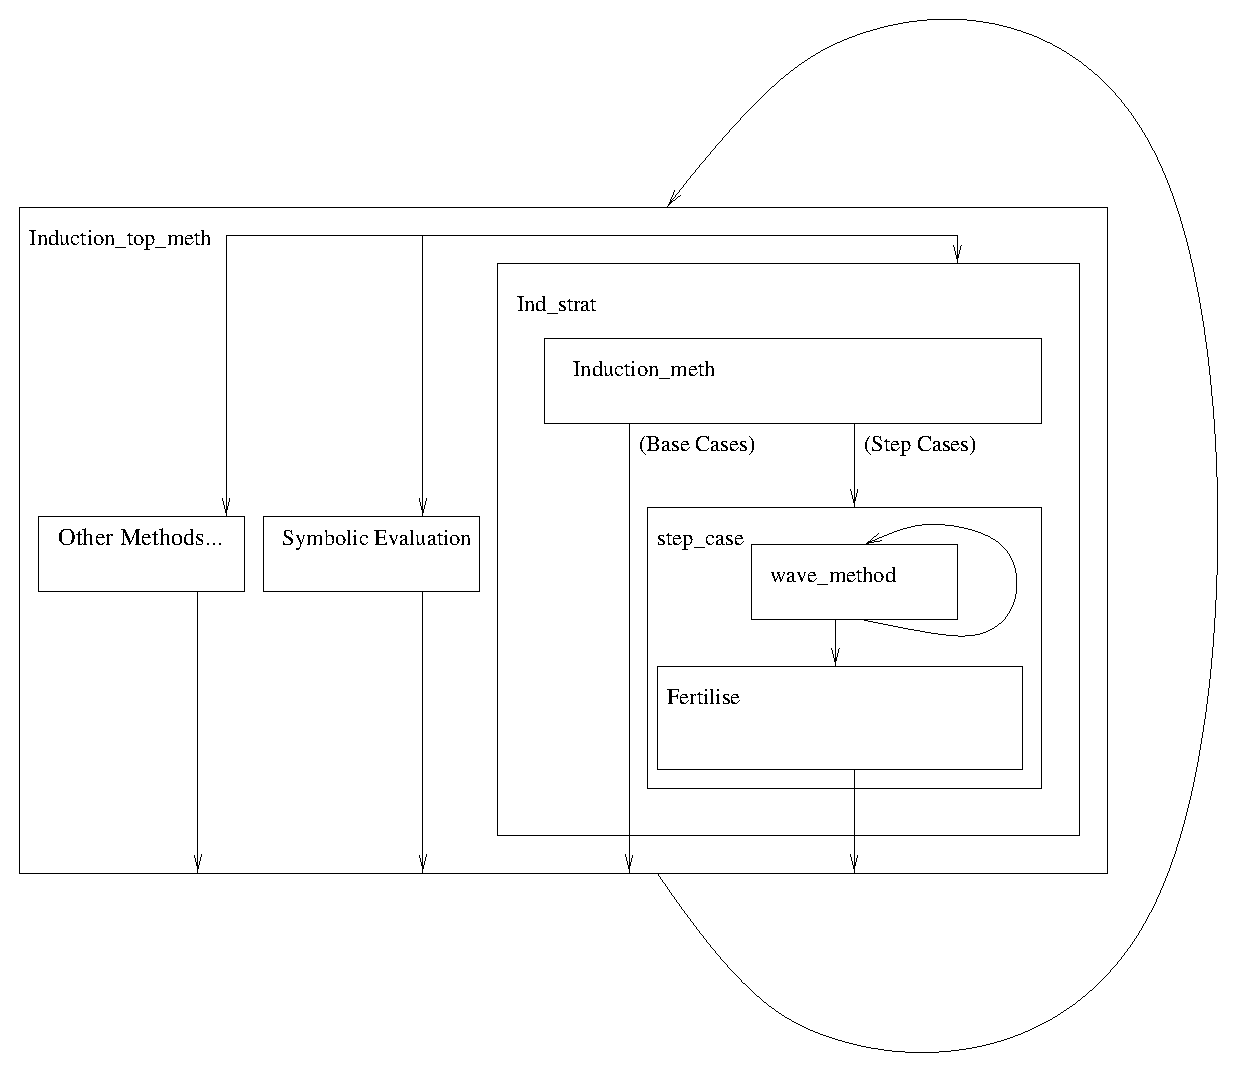
\epsfig{file=ind_strat.eps, width=4.8in}
\end{center}
\caption{The Proof Strategy for Induction}
\label{fig:induction_strategy}
\end{figure}
This is implemented as a selection of atomic and compound methods.
The diagram shows a top level repeat which attempts a disjunction of
methods.  These include basic tautology checking, generalisation of
common subterms and also symbolic
evaluation and the induction strategy ({\tt ind\_strat}).  Within the
induction strategy, the induction method
performs ripple
analysis~\cite{ind-chap-ref2} to choose an induction scheme (from a
selection specified in \lclam's theories) and produces subgoals for
base and step cases.  The base cases
are passed out to the repeat of the top level strategy.
The step cases are annotated with \emph{skeletons} and
\emph{embeddings} (described 
below) and then the wave method is repeatedly applied to them followed 
by fertilisation (exploitation of the induction hypothesis).
Annotations are then removed.  The methods ({\tt set\_up\_ripple} and
{\tt post\_ripple}) which place and remove annotations are omitted
from the diagram.  The results are then passed out to the top level
strategy again.  The process terminates when all subgoals have been
reduced to \emph{true} (or \emph{false} in the case of failure).

We will discuss the \method{wave\_method} in more detail since it was
a new formulation of this method we wished to investigate.  The wave
method embodies the rippling heuristic.  Rippling was first introduced
in~\cite{pub567}.  We use the theory as presented by Smaill \&
Green~\cite{pub799} who proposed a version that naturally coped with
higher-order features.  Rippling steps apply rewrite rules to a target
term which is associated with a skeleton and an embedding
that relates the skeleton to the target term (e.g.
rippling\index{rippling} rewrites an induction conclusion which has an
induction hypothesis embedded in it).  In the present context, we make
use of higher order rewriting, in the style of \cite{Fel92}.  After rewriting a new embedding of the skeleton into the rewritten term is calculated.  There is
a measure on embeddings and any rewriting step must reduce this
\emph{embedding measure} (written as $<_{\mu}$).  This is a
generalisation of the original version of rippling that used annotated
\emph{wave rules} to rewrite annotated terms.

Rippling is terminating~\cite{BasinWalsh96}.  Rippling either moves
differences outwards in the term structure so that they can be
cancelled away or inwards so that the differences surround a
universally quantified variable (or \emph{sink}).  If it is possible
to move differences inwards in this way the embedding is said to be
\emph{sinkable}.  The measure on embeddings allows differences that
are being moved outwards to be moved inwards but not vice versa --
this is at the heart of the guarantee of termination.

The \method{wave\_method} method has five preconditions.  It finds a
rewrite rule that rewrites the goal.  It then checks that there is
still an embedding of the skeleton into the rewritten goal and that
this new embedding is less, according to the embedding measure, than
the original embedding.  It checks that the embedding is sinkable and
that any conditions for the application rule are trivial.  This is
shown in figure~\ref{fig:wave_method}.  
%Sinkability is not necessary
%for termination but it is a useful further heuristic for guiding the
%proof.
\begin{figure}[htb]
\pageline
% \vspace{1mm}
\begin{center}
\begin{center}
\textbf{Input}

$$ripple\_goal(H \vdash G, S, E).$$
where $ripple\_goal$ is a triple of a sequent, a skeleton, $S$ and an
embedding, $E$, of that skeleton into the goal, $G$.
\end{center}
\begin{center}
\textbf{Preconditions}
\end{center}

\begin{enumerate}
\item The conditional
  rewrite rule \emph{Rule}, $Cond \imp X \rewrites Y$ instantiated
  with some substitution $\sigma$, applies to $G$
  and rewrites it to $G'$.
\item There is an embedding $E'$ that embeds $S$ in $G'$.
\item $E' <_{\mu} E$.
\item $\sigma(Cond) = True$ or $\sigma(Cond) \in H$.
\item $E'$ is sinkable.
\end{enumerate}
\begin{center}
\textbf{Output}
\end{center}
$ripple\_goal(H \vdash G', S, E')$
\end{center}
\vspace{1mm}
\pageline
\caption{The Wave Method}
\label{fig:wave_method}

\end{figure}
The method will backtrack\index{backtracking} in order to try to
satisfy all requirements, and if it is successful returns a new goal.

%The main advantages of rippling is that it allows an equation
%to be treated as a rewrite in both directions without loss of
%termination and provides useful information for automatically patching 
%failed proof attempts.  These abilities were not required in this case 
%studies and all the proofs went through automatically using 
%symbolic evaluation instead of rippling.  However, our intention was
%to test the higher-order presentation of rippling \emph{not} to justify 
%its necessity in the case of ordinals.

\section{Embeddings}
\label{embeddings}
We review here the notion of embeddings from Smaill \&
Green \cite{pub799}.  These provide the higher-order framework for
rippling used in this paper.

Embeddings are described by a tree data structure.  Embedding trees
describe how a \emph{skeleton} embeds in a term, called
the \emph{erasure}.  The nodes in an embedding tree
can be viewed as labels on the nodes in the term tree of the skeleton.
These labels contain addresses and directions.  The directions are
used during rippling as outlined above.  The addresses
are the addresses of nodes in the term tree of the erasure which
correspond to that node in the skeleton.  Term trees represent
function application and $\lambda$-abstraction explicitly as nodes with
constant and variables symbols appearing only at the leaves of the
tree.  Our implementation also contains tuple nodes for lists of
arguments to functions but these are not necessary to the theory.
Embeddings do not annotate $\lambda$-abstraction nodes.  Where an
embedding matches a variable in the skeleton to one in the erasure it
indicates that they are $\alpha$-convertible.
It is the ability to coherently handle
$\lambda$-abstractions which was particularly valuable in this
experiment.  The ability to handle difference occuring within functions as well
as the arguments to functions is also an extension of the previous
calculus.

\begin{example}
Consider embedding the term $\lam{x} f(x)$ into the term
$\lam{y} \lam{x} (f(y) + x)$. We 
do this as in figure~\ref{fig:embed}.  The two terms are shown 
as trees with branches represented by solid lines.  The address of
each node is given ($\lambda$-abstraction nodes do not carry
addresses).  The embedding appears
between them as an  
embedding tree with dashed lines -- the address label of
the nodes is 
also shown.  The dotted arrows illustrate how the embedding tree links 
the two terms.

\begin{figure}[htb]
\begin{center}
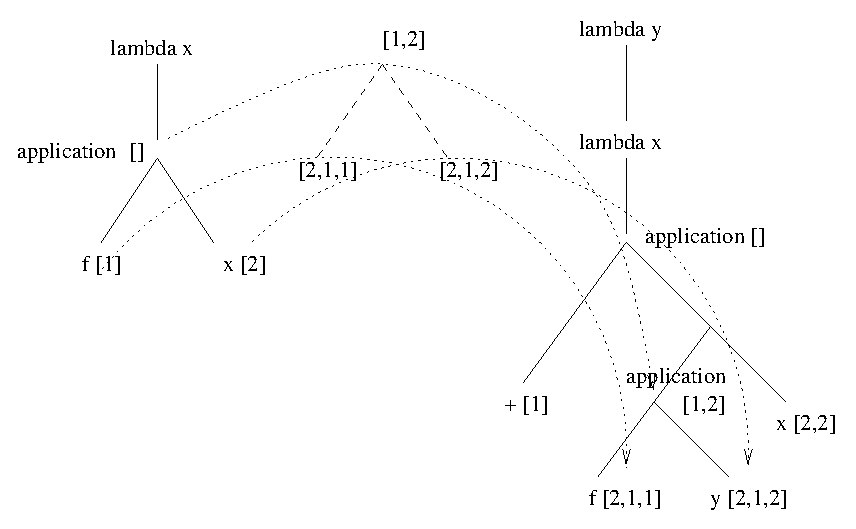
\epsfig{file=embed.eps, width=3in}
\end{center}
\caption{An Embedding}
\label{fig:embed}
\end{figure}

The embedding tree for this is  (node [1, 2] [(leaf
[1, 1, 1]) (leaf [2, 1, 2])])).  This states
that the function 
application at the top of $f(x)$ matches with the node at
address [1, 2] of $f(y) + x$ (i.e. the application involving $+$ has
been bypassed), that the
function symbol $f$ matches the sub term at [2,1,1] (i.e. $f$)
and $x$ matches $y$ (i.e.\ the bound variables can be consistently
renamed in either (or both) terms so that they are identical).

The annotations originally used in rippling 
are still useful for presentation.  Annotations consist of contexts
(expressions 
with holes) indicated by a wave front (box) with a directional arrow.
The holes in the context are wave holes (i.e. they are filled with an
expression which is underlined). The skeleton is everything
that appears outside wave fronts, or in wave holes. 
So the above embedding can be
presented as 
$$
\lam{x} \wfout{\lam{y} \wh{f(y)} + x}.
$$

NB.  It is important to remember that the annotations do not actually
exist in the implementation which records instead the 
skeleton and embedding\footnote{In fact \lclam\ maintains a list of
possible embeddings 
during rippling since there may be more than one way to embed the
induction hypotheses into the conclusion.  For convenience we assume
here there is only one.}.  
In some cases it is less easy to use the
traditional annotations to represent embeddings, particularly when dealing
with $\lambda$-abstrations which are ignored by the embedding trees.
You can see that in the above the bound variables in the skeleton 
are assumed to have been appropriately renamed already.
These 
annotations are just a presentational convenience.
\end{example}

\section{Logics}
You will note that the proof strategy for induction calls the {\tt
  taut}\index{taut} method for tautology checking.  This may vary
depending upon whether constructive or classical logic (for instance)
is being used.  As a result the basic ``build'' of the induction
theory\index{induction theory} in \lclam\ does not specify how the
{\tt taut} method or logical constants such as {\tt
  forall}\index{forall} or {\tt and}\index{and} should be treated by
the system.  It simply asserts that they exist.  Additional files, of
which the {\tt constructive\_logic}\index{constructive\_logic} theory
can then be created to provide the necessary details.

\section{Arithmetic, Natural Numbers and Lists}
There are a number of built-in theories dealing with natural number
and list theorems.  Standard functions and goals can be found in the
{\tt arithmetic}\index{arithmetic} theory and the {\tt
  objlists}\index{objlists} theory.  Further functions can be found in 
{\tt list\_benchmarks}\index{list\_benchmarks}, {\tt
  map\_benchmarks}\index{map\_benchmarks} and the {\tt
  clam\_corpus}\index{clam\_corpus} theories (there are 3 clam corpus
theory files).

\section{Mutual induction}
\noindent 
This module was written for the MFOTL group based at Liverpool.  The
method \texttt{alexei\_meth} in
\texttt{theories/mutual\_induction.mod} implements the following proof
rule.  It is a variant of a mutual induction rule suitable for
treatment of arithmetical translations of temporal formulae:

\vspace{0.5cm}

$ \forall y \forall \bar{x} A_{1}(y, \bar{x}) \Rightarrow B_{1}(s(y), \bar{x})$

$\forall y \forall \bar{x} A_{2}(y, \bar{x}) \Rightarrow B_{2}(s(y), \bar{x})$

$\ldots $

$\forall y \forall \bar{x} A_{n}(y, \bar{x}) \Rightarrow B_{n}(s(y), \bar{x})$

\vspace{-1mm}
$\underline{\qquad\qquad\qquad\qquad\qquad\qquad\qquad\qquad\qquad\qquad}$
 
\vspace{1mm}
$\forall u. u > t \Rightarrow \varphi(u)$ 

\vspace{5mm}
\noindent
with the side conditions: 

\[\begin{array}{l} 
\exists \bar{x}  (A_{1}(t,\bar{x}) \vee A_{2}(t, \bar{x}) \vee \ldots \vee 
A_{n}(t,\bar{x})) \\
\\
\forall y \forall \bar{x} (B_{i}(y, \bar{x}) \Rightarrow \varphi(y)) , i=1, \ldots, n \\
\\
\forall y \forall \bar{x} \exists \bar{z} ( B_{i}(y, \bar{x}) 
\Rightarrow \bigvee_{j=1\ldots n} A_{j}(y,\bar{z})) ,  i=1 \ldots, n 
\end{array}\]

\noindent
where $A_{i}$ and $B_{i}$ are arbitrary first-order formulae, $t$ is
an arbitrary arithmetical term, s is the successor function symbol,
$\Rightarrow$ is implication, $\bar{x}$ is a sequence of
variables, and $y$ is a (numerical) variable of type \texttt{nat}.  $n$ is
not fixed, so we can deal with arbitrary lists of premises in the rule.

\noindent
Since the rule is generally used in backward reasoning, 
one can present its application as follows: \\

\noindent
Given a goal sequent $H \vdash \psi$ with $\psi$ being of the form of
the conclusion of the above rule, the method generates some subset
$H'$ of $H$ matching the premises of the rule and generates the
associated side conditions as new subgoals.  These subgoals are
then resolved by application of some other methods (for first-order
reasoning). \\

\noindent
At present the method simply chooses the maximal matching subset of
hypotheses.  Probably some optimization for iteration over subsets
will be needed later.

\noindent{\bf Example:} \\

Given:   
\[\begin{array}{l}
\forall x, y (A(y,x) \Rightarrow B(s(y),x)) \\
\forall x, y (C(y,x) \Rightarrow D(s(y),x)) \\
\forall x (A(0,x) \lor C(0,x)) \\
\forall x,y (B(y,x) \Rightarrow C(y,x)) \\
\forall x,y (D(y,x) \Rightarrow (A(y,x) \lor C(y,x))) 
\end{array}\]

\vspace{-1mm}
$\underline{\qquad\qquad\qquad\qquad\qquad\qquad\qquad\qquad\qquad\qquad\qquad}$

Prove: 
\[\forall y > 0  \exists x (B(y,x) \lor D(y,x)) \]
 
Side conditions to prove (taking the set of first two hypotheses and the
conclusion):

\[\begin{array}{l}
\exists x (A(0,x) \lor C(0,x))\\
\\
\forall y \forall x (B(y,x) \Rightarrow  \exists z (B(y,z) \lor D(y,z))) \\
\\
\forall y \forall x (D(y,x) \Rightarrow  \exists z (B(y,z) \lor D(y,z))) \\
\\
\forall y \forall x \exists z (B(y,x) \Rightarrow A(y,z) \lor C(y,z)) \\
\\
\forall y \forall x \exists z (D(y,x) \Rightarrow A(y,z) \lor C(y,z)) \\
\end{array}\]
\newcommand{\lyacc}{$\lambda$yacc\xspace}

\chapter{Compiling Theories to \lclam}\label{compiler}

%\author{Ewen Denney}

\section{Introduction}

This chapter describes the current state of the \lclam theory
compiler.  It develops the idea that a logic can be presented in a
high-level declarative style, and then {\em compiled} down into a more
procedural implementation-specific language.

The reasons for wanting to do this are:
\begin{itemize}
\item the user-unfriendliness of the current \lclam format
\item to avoid errors that can arise when entering axioms and
  inferences as low-level rewrites and methods
\item (ultimately) to aim for a logic-independent planner by factoring out
  logic-specific code
\item since a high-level representation of logics and theories, rather than
  one which is hard-wired into a low-level implementation, is easier
  to communicate.
\end{itemize}

In our case, of course, the procedural language is \lclam's format for
the paraphernalia of proof planning (expressed in HOAS) in \lprolog;
for declarative language, we simply make up our own user-friendly
syntax for declarations, inference rules, and the like.


The compiler has two modes of use: online, using the {\tt add\_theory}
command during \lclam's normal command loop, and offline, generating a
separate \lclam theory file.  The offline mode is currently deprecated
but is described here as it helps understand the general compilation
process and may prove useful in the future.

\section{Online Mode}

The command
$${\tt add\_theory} \mbox{\em ``theory-file''}$$
will read in the file
{\em theory-file}, check its well-formedness, and generate the
appropriate user-defined constants.

For example, the file {\tt simpletheory}:
\begin{verbatim}
Theory Nsa.
Use Logic arithmetic.

type real.
type hyperreal.
$
\end{verbatim}
gives the following results:
\begin{verbatim}
lclam:
add_theory "simpletheory".
Trying ...Scanning for tokens...
Tokenizer stopped after line 6
Parsing...
Successfully parsed
Checking well-formedness...
Type real
Type hyperreal
Theory is well-formed
Importing lclam declarations...
Successfully processed
Done
Done
lclam:
\end{verbatim}
We can now use the query commands to check that the definitions have been made
correctly.
\begin{verbatim}
lclam:
query_osyn (user_theory "nsa") (user_object "real") X.
default
user_theory "nsa"
real
universe
lclam:
\end{verbatim}

A more complex example of a theory file can be seen in
Section~\ref{theory}.

\section{Offline Mode}

We describe here how a user can use the files {\tt
  envgrammar.\{sig,mod\}} and\linebreak 
{\tt postprocess.\{sig,mod\}} in the
{\tt compiler} directory to parse a theory file written in concrete
syntax and generate a \lclam theory file.

We first explain how to use the compiler, and in the following
sections, explain the workings of the compiler in case the user wants
to alter it.

The phases of such a logical compilation are much the same as in the
compilation of programs: parsing of concrete into abstract syntax
(Section \ref{parsing}), a well-formedness check (Section
\ref{well-formedness}), and then code generation (Section
\ref{generation}). We give the grammar for theory files (Section
\ref{grammar}), and examples of concrete syntax (Section \ref{theory}) and
the corresponding \lclam (Section \ref{lclam}).


\subsubsection{Using the Compiler}\label{makefile}

First, edit the {\tt Makefile}, if necessary, to alter the paths appropriately.

Then, generate the parser by
\begin{alltt}
make envparser
\end{alltt}
Next, do
\begin{alltt}
make postprocess
\end{alltt}

If the theory file is {\tt theoryfile}, then the command
\begin{alltt}
parsefile "theoryfile" X.
\end{alltt}
will bind to $\tt X$ the abstract syntax that results from parsing
this file. This might be useful to you if you just want access to the
higher-order abstract syntax form of an expression.

Here, {\tt theoryfile} is the file with concrete syntax which you can,
of course, change and rename. Note that the underlying parser, \lyacc,
requires this file to terminate with a {\tt \$}.

The command
\begin{alltt}
process_file "theoryfile"
\end{alltt}
will parse the file, check its well-formedness, and output the
appropriate \lclam files. The names of the files are determined by
the line
\begin{alltt}
Theory <name>.
\end{alltt}
in the theory file, which results in {\tt <name>theory.\{sig,mod\}}. 

Finally, you then have to fit these files in with your version of
lambda clam (by setting the appropriate accumulates) and compile the
whole system. Note that the compilation files themselves should not be
compiled with \lclam.


\subsection{Parsing}\label{parsing}

The logic file is first parsed into abstract syntax. The parser is
implemented using 
\lyacc\footnote{See {\tt http://www.cs.hofstra.edu/\~{ }cscccl/parsergen/.}}, 
a parser-generator written in \lprolog, due to Chuck Liang. It
generates bottom-up {\em shift-reduce} parsers, which can be less
intuitive than top-down parsers, but are more efficient.

The user specifies their logic by writing various predicates and rules
in a \lprolog file, which accumulates the \lyacc files.

\begin{enumerate}
\item Declare grammar symbols for the abstract syntax for each nonterminal.
\item Declare the terminals.
\item Give concrete syntax for the terminals using {\tt printname}.
\item List the terminals, and nonterminals.
\item Set {\tt ntnum} to the number of nonterminals plus 1.
\item
Give the parse rules, with semantic actions to construct
the abstract syntax.

For example, rules giving the syntax for axiom declarations are
\begin{verbatim}
 rule ((syn_decl_gs D5) ==> 
        [axiom_decl_gs S7 H1 Z7]) (D5 = axiom_decl S7 H1 Z7),

 rule ((axiom_decl_gs S5 H2 Z5) ==> 
        [axiomt, axiom_name I6, qprop_gs Z3, periodt]) 
                                (S5 = I6, Z5 = Z3, H2 = []),
\end{verbatim}
The {\tt rule} construct combines a production with a semantic action.
\item
Give precedence rules.
\item Supply freshcopy clauses for non-nullary nonterminals.
\end{enumerate}


This file is compiled, and then executed. Then, a generate parser
command is called, which, assuming \lyacc accepts the file, generates
{\em another} file. This file is then compiled to give the parser, all
of which takes about a minute in total.


\subsection{Well-formedness}\label{well-formedness}

A consequence of the fact that the semantic actions attached to \lyacc
parse rules cannot contain implications (and that \lprolog does not
have assertions), is that well-formedness of the resulting abstract
syntax has to be checked in a separate pass.

However, logically inspired manipulation of terms such as this is what
\lprolog does best.  For example, well-formedness of existentials and
abstractions is checked by
\begin{verbatim}
well_formed_assertion (app exists (tuple [T, abs P])) :-
        well_formed_type T,
        pi X \ (new_const X T) => well_formed_assertion (P (user_object X)). 

well_typed_term (ty_abs T L) (T arrow U) :-
        well_formed_type T,
        pi X \ (new_const X T) => well_typed_term (L (user_object X)) U.
\end{verbatim}
Since declarations are `first-class' in \lprolog, \lprolog's context
mechanism can be used for managing declarations.

\begin{verbatim}
well_formed_decls ((inference_decl S Hyps H2 C2)::Ds) :-
        well_formed_decl (inference_decl S Hyps H2 C2),
        ((new_inference S) => well_formed_decls Ds).

well_formed_decl (inference_decl S Hyps H2 C2) :-
        not (new_inference S),
        map_pred2 group_assertions Hyps Ass,
        all_pred well_formed_assertions Ass,
        ly_append H2 [C2] Ps2,
        well_formed_assertions Ps2,
        M is "Inference " ^ S ^ "\n",
        print M.
\end{verbatim}
There are no error messages at present.

\subsection{Generation of \lclam}\label{generation}
Once the theory file has been parsed into abstract syntax and checked
for well-formedness, it is converted to \lclam format and written to a
file. Constructing the appropriate higher-order abstract syntax was
done during parsing, so this stage is mainly concerned with
abstracting over the variables, and converting propositions to
rewrites and methods.

The syntax comprises a list of declarations, each of which is
converted to the corresponding \lclam entity.

\begin{alltt}
% decl2lclam {\it +sig-file +mod-file +theory-name +logic-name +declaration}

type decl2lclam  out_stream -> out_stream -> string -> string -> syn_decl -> o.
\end{alltt}
A syntactic declaration is one of: type, typed constant, axiom,
inference, conjecture, predicate symbol, definition.  The interesting
cases are axiom and inference rules. We convert axioms to rewrite
rules, and inferences to methods.

An example of an axiom is
\begin{verbatim}
axiom ax1 [y:nat |- forall f:nat->nat. f = (x:nat \ (f y))].
\end{verbatim}
This is parsed as
\begin{verbatim}
axiom_decl "ax1" (otype_of (user_object "y") nat :: nil) 
   (app forall (tuple ((nat arrow nat) :: 
         abs (W1\ app eq 
          (tuple (W1 :: ty_abs nat (W2\ app W1 (user_object "y")) :: nil))) ::
 nil)))
\end{verbatim}
and converted to the rewrite rule
\begin{verbatim}
axiom nsa ax11 ltor (trueP) 
   (app forall 
     (tuple ((nat arrow nat) :: 
       abs (W1\ app eq (tuple (W1 :: ty_abs nat (W2\ app W1 _107597) :: nil)))
 :: nil))) 
    (trueP).
\end{verbatim}


For inference rules, the system generates preconditions to check
for required antecedents in the conclusion, and to construct the
antecedents of the hypotheses. The succedent of the conclusion is
recorded in the form of the method input, and the succedents of the
hypotheses appear in the output goal.

For example, the inference rule
\begin{verbatim}
inference and_l [G,A,B,G' |- P / G, A /\B |- P]
\end{verbatim}
parses to abstract syntax
\begin{verbatim}
(inference_decl "and_l"
[(pair [user_object "G", user_object "A", user_object "B", user_object "G'"] 
       (user_object "P"))]
[user_object "G", (app and (tuple [user_object "A", user_object "B"])), 
user_object "G'"] (user_object "P"))
\end{verbatim}
which is converted to the atomic method
\begin{verbatim}
atomic nsa and_l
        (seqGoal (H >>> (_9055)))
        (sublist (app and (tuple (_9072 :: _9088 :: nil)) :: nil) H, 
        replace_in_hyps H (app and (tuple (_9072 :: _9088 :: nil))) 
                             (_9072 :: _9088 :: nil) H1)
        true
        seqGoal (H1 >>> _9055)
        notacticyet.
\end{verbatim}
The inference rule
\begin{verbatim}
inference and_r [G |- A ; G |- B / G |- A /\B]
\end{verbatim}
parses to abstract syntax
\begin{verbatim}
(inference_decl "and_r"
[(pair [user_object "G"] (user_object "A")),
(pair [user_object "G"] (user_object "B"))]
[user_object "G"] (app and (tuple [(user_object "A"), (user_object "B")]))
)
\end{verbatim}
and converts to
\begin{verbatim}
atomic nsa and_r
        (seqGoal (H >>> (app and (tuple (_5035 :: _5052 :: nil)))))
        (H =  H1, H =  H2)
        true
        seqGoal (H1 >>> _5035) ** seqGoal (H2 >>> _5052)
        notacticyet.
\end{verbatim}


\subsection{Theory Grammar}\label{grammar}

Identifiers can contain underscores but not hyphens. A theory begins
with a declaration of its name, and the logic it uses. The logic name
is not used, but must be entered for syntactic correctness.

\begin{verbatim}
Theory-declaration ::= 
        'Theory' Id '.'
        'Use Logic' Id '.'
        (Declaration '.')*

Declaration ::= Constant-declaration
                | Type-declaration
                | Axiom-declaration
                | Inference-declaration
                | Conjecture-declaration
                | Predicate-declaration
                | Definition


Constant-declaration ::= 'const' Id Type

Type-declaration ::= 'type' Id

Axiom-declaration ::= 'axiom' Id Prop | 'axiom' Id '[' Sequent ']' 

Inference-declaration ::= 'inference' Id '[' Sequents '/' Sequent ']'

Conjecture-declaration ::= 'conjecture' Id '[' Sequent ']'

Predicate-declaration ::= 'predicate' Id Type+

Definition ::= 'define' 'const' Id ':' Type '=' Term
             | 'define' 'type' Id '=' Type

Sequents ::= (Sequent ';')* Sequent

Sequent ::= Assumptions '|-' Prop

Assumptions ::= (Assumption ',')* Assumption

Assumption ::= Prop | Id ':' Type

Prop ::= 'forall' Id ':' Type '.' Prop
       | 'exists' Id ':' Type '.' Prop
       | Prop '/\' Prop
       | Prop '\/' Prop
       | Prop '=>' Prop
       | '<' Term '=' Term '>'
       | '(' Prop ')'
       | Id
       | Id '{' Term '}'

Type ::= nat | bool | '(' Type ')' | Type '->' Type | Type '#' Type | Id

Term ::= Id
       | (Id ':' type '\' Term ')'
       | '<' Term Term '>'
\end{verbatim}

\subsection{Theory file}\label{theory}
\begin{verbatim}
Theory Nsa.
Use Logic Thol.

type real.
type hyperreal.
const z nat.
const f nat->nat#bool.

axiom sch2 [x:nat |- <x=x>].
axiom sch3 [x:nat, y:nat |- <x=y>].
axiom sch4 [x:nat, y:nat, <x=y> |- <y=x>].
axiom ax1 [y:nat |- forall f:nat->nat. <f = (x:nat \ <f y>)>].
axiom exax exists x:nat. <x=x>.
axiom badax [true, x:nat |- <x=x>].

conjecture conj1 [x:nat |- forall y:nat . <x=y>].
inference inf1 [true |- false / true, x:nat |- <x=x>].

axiom qs (forall x:nat. (exists y:nat. <x=y>)) => true.

conjecture conj2 [x:hyperreal |- exists y:hyperreal . <x=y>].

predicate even : nat.
predicate close_to : hyperreal, real.

inference easy_inf [true|-true; false|-false / x:nat |- <x=x>].

axiom pred_in_prop even{z}.

define type real_pair = real#real.

define const n:nat#bool = <f z>.

define const m:nat = z.

axiom false_e [G1, false, G2 |- P].

inference and_r [G |- A; G |- B / G |- A /\ B].

inference and_l [G1,A,B,G2 |- P / G1, A /\B,G2 |- P].

inference or_l [G,A |- P; G,B |- P / G, A\/B |- P].
\end{verbatim}

\subsection{Generated \lclam}\label{lclam}
\begin{verbatim}
module nsatheory.

all_pred P nil.
all_pred P (H::T) :- P H, all_pred P T.
sublist Xs Ys :- all_pred (X\ (member X Ys)) Xs.

has_otype nsa real universe.
has_otype nsa hyperreal universe.
has_otype nsa z (nat).
has_otype nsa f (nat arrow tuple_type (nat :: bool :: nil)).
axiom nsa sch21 ltor (trueP) (_135695) (_135695).

axiom nsa sch22 ltor (trueP) (app eq (tuple (_137129 :: _137129 :: nil))) 
(trueP).

axiom nsa sch31 ltor (trueP) (_137732) (_137749).

axiom nsa sch41 ltor (app eq (tuple (_139400 :: _139383 :: nil))) (_139383) 
(_139400).

axiom nsa sch42 ltor (app eq (tuple (_144856 :: _144839 :: nil))) (app eq 
(tuple (_144839 :: _144856 :: nil))) (trueP).

axiom nsa ax11 ltor (trueP) (app forall (tuple ((nat arrow nat) :: abs (W1\ 
app eq (tuple (W1 :: ty_abs nat (W2\ app W1 _147505) :: nil))) :: nil))) 
(trueP).

axiom nsa exax1 ltor (trueP) (app exists (tuple (nat :: abs (W1\ app eq (tuple
 (W1 :: W1 :: nil))) :: nil))) (trueP).

axiom nsa badax1 ltor (trueP) (_148474) (_148474).

axiom nsa badax2 ltor (trueP) (app eq (tuple (_149926 :: _149926 :: nil))) 
(trueP).

top_goal nsa conj1 [(otype_of (user_object "x") nat)] (app forall (tuple (nat 
:: abs (W1\ app eq (tuple (user_object "x" :: W1 :: nil))) :: nil))).
atomic nsa inf1
        (seqGoal (H >>> (app eq (tuple (_152632 :: _152632 :: nil)))))
        (sublist (trueP :: otype_of (user_object "x") nat :: nil) H)
        true
        (seqGoal (H1 >>> falseP))
        notacticyet.

axiom nsa qs1 ltor (trueP) (trueP) (app forall (tuple (nat :: abs (W1\ app 
exists (tuple (nat :: abs (W2\ app eq (tuple (W1 :: W2 :: nil))) :: nil))) :: 
nil))).

axiom nsa qs2 ltor (trueP) (app imp (tuple (app forall (tuple (nat :: abs (W1\
 app exists (tuple (nat :: abs (W2\ app eq (tuple (W1 :: W2 :: nil))) :: 
nil))) :: nil)) :: trueP :: nil))) (trueP).

top_goal nsa conj2 [(otype_of (user_object "x") (user_object "hyperreal"))] 
(app exists (tuple (user_object "hyperreal" :: abs (W1\ app eq (tuple 
(user_object "x" :: W1 :: nil))) :: nil))).
atomic nsa easy_inf
        (seqGoal (H >>> (app eq (tuple (_156487 :: _156487 :: nil)))))
        (sublist (otype_of (user_object "x") nat :: nil) H, replace_in_hyps H 
(otype_of (user_object "x") nat) (falseP :: nil) H1, replace_in_hyps H 
(otype_of (user_object "x") nat) (trueP :: nil) H2)
        true
        (seqGoal (H1 >>> trueP) ** seqGoal (H2 >>> falseP))
        notacticyet.

axiom nsa pred_in_prop1 ltor (trueP) (app (user_object "even") (user_object 
"z")) (trueP).

definition nsa real_pair0 trueP (tuple_type (user_object "real" :: user_object
 "real" :: nil)) real_pair.
definition nsa n0 trueP (app (user_object "f") (user_object "z")) n.
definition nsa m0 trueP (user_object "z") m.
atomic nsa false_e
        (seqGoal (H >>> (_25170637)))
        (sublist (falseP :: nil) H)
        true
        trueGoal
        notacticyet.

atomic nsa and_r
        (seqGoal (H >>> (app and (tuple (_162845 :: _162862 :: nil)))))
        (true, H =  H1, H =  H2)
        true
        (seqGoal (H1 >>> _162845) ** seqGoal (H2 >>> _162862))
        notacticyet.

atomic nsa and_l
        (seqGoal (H >>> (_186518)))
        (sublist (app and (tuple (_186535 :: _186551 :: nil)) :: nil) H, 
replace_in_hyps H (app and (tuple (_186535 :: _186551 :: nil))) (_186567 :: 
_186535 :: _186551 :: _186583 :: nil) H1)
        true
        (seqGoal (H1 >>> _186518))
        notacticyet.

atomic nsa or_l
        (seqGoal (H >>> (_197214)))
        (sublist (app or (tuple (_197231 :: _197247 :: nil)) :: nil) H, 
replace_in_hyps H (app or (tuple (_197231 :: _197247 :: nil))) (_197247 :: 
nil) H1, replace_in_hyps H (app or (tuple (_197231 :: _197247 :: nil))) 
(_197231 :: nil) H2)
        true
        (seqGoal (H1 >>> _197214) ** seqGoal (H2 >>> _197214))
        notacticyet.

end

\end{verbatim}



%=========================
%%   Systemnamen
%%=========================

\newcommand{\Nat}{{\mathchoice{\displaystyle\rm I\hskip-0.21em N}%
{\textstyle\rm I\hskip-0.21em N}%
{\scriptstyle\rm I\hskip-0.14em N}%
{\scriptscriptstyle\rm I\hskip-0.14em N}}}
%%%%%%%%%%%%%%%%%%%%%%%%%%

\def\eps{\epsilon}
\def\name#1{#1}
\def\xspace{}
\def\activemath{{\it ActiveMath}}
\def\analytica{{\it Analytica}}
\def\automath{AUTOMATH}
\def\bliksem{{\it Bliksem}}
\def\chip{\mbox{CHIP}\xspace}
\def\chorus{Chorus}
\def\clamlite{{CLAM-Lite}}
\def\clos{{{\small CLOS}}}
\def\commonlisp{{{\footnotesize COMMON LISP}}}
\def\corba{{\sc Corba}}
\def\cosie{${\cal C}o{\cal SIE}$}

\def\davinci{\mbox{\sc daVinci}\xspace}
\def\declame{{{\small DECLAME}}}
\def\discount{{DISCOUNT}}
\def\doris{DORIS}
\def\eclipse{ECL$^i$PS$^e$}
\def\eqp{EQP}
\def\eprover{{\sf E}}

\def\fipa{{\sf FIPA}}
\def\fscos{${\cal FSC}o{\cal S}$}
\def\HOL{{$\cal HOL$}}
\def\hr{{\sf HR}}
\def\http{{\sf http}}

\def\ilf{{ILF}}
\def\ilog{ILOG}
\def\imply{IMPLY}
\def\imps{\mbox{\sc IMPS}\xspace}
\def\isabelle{\mbox{\it Isabelle}\xspace}

\def\keim{{\small\bf KEIM}}
\def\KEIM{{\small\bf KEIM}}
\def\kimba{{\sf Kimba}}
%\def\kqml{{\sc Kqml}}
\def\kqml{KQML}
\def\larks{LARKS}
\def\mathml{{\sc MathML}}
\def\oants{{\sf OANTS}}
\def\omrs{{\sc OMRS}}
\def\openmath{{\sc OpenMath}}
\def\omdoc{{OMDoc}} %\protect\omdocaux}
\def\omdocaux{\sc O\kern-1.6ex\raisebox{.4ex}{{\tiny M}}Doc}
\def\prosper{{\sc Prosper}}
\def\pvs{PVS}
\def\setheo{{SETHEO}}
\def\teamwork{{\sc Teamwork}}
\def\techs{{TECHS}}
\def\waldmeister{Waldmeister}
\def\xml{XML}
\def\xsl{{\sc Xsl}}

\def\lams{{\sf LaMS}}
\def\leo{\mbox{${\cal LEO}$}\xspace}
\def\lineq{{\sc LinEQ}}
\def\lisp{{\footnotesize LISP}}
%\def\loui{\mbox{{\sc L}$\Omega${\sc UI}}\xspace}
\def\LOUI{\mbox{\sc L}{\sc ovely} {$\Omega${\sc mega}} {\sc U}{\sc ser} {\sc I}{\sc nterface}}

\def\gap{GAP}
\def\cocoa{CoCoA}
\def\lba{LBA}
\def\lclam{\mbox{$\lambda$\--Clam}}
\def\mace{MACE}
\def\magma{{\sc MagMa}}
\def\maple{{\sc Maple}}
\def\mass{{\sc Mass}}
\def\mathematica{{\it Mathematica}}
\def\mathpert{{\it Mathpert}}
\def\mathweb{Math\-Web}
\def\mathwebsb{Math\-Web-SB}
\def\mathagent{\mbox{\sc MathAgent}\xspace}
\def\mbase{{\sc MBase}}
\def\mkrp{{MKRP}}
\def\mosh{\sc MoSh}
\def\mozart{\sc Mozart}
\def\multi{MULTI}
\def\mycas{\mbox{$\mu$\hspace{.2em}${\cal CAS}$}}
\def\MYCAS{\mbox{$\mu${\sc CAS}}}
\def\myCAS{\mbox{$\mu${\sc CAS}}}

\def\ND{{\small\bf ND}}
\def\nuprl{{Nuprl}}
\def\octopus{\mbox{$\Omega${\sc cTOpus}}\xspace}
\def\OMEGA{$\Omega${\sc mega}}
\def\omws{OMWS}
\def\otter{{\sc Otter}}
\def\oyster{{\mbox{\rm O\kern-.12em\raise.39ex\hbox{\sc y}\kern-.07emS\kern-.39em\raise.39ex\hbox{\sc t}\kern-.15em\hbox{\sc e}R}}}
\def\oz{{\sc Oz}}

\def\pds{PDS}
\def\POST{{\mbox{$\cal POST$}}}
\def\post{{\POST}}
\def\Post{{\POST}}
\def\prolog{PROLOG}
\def\lprolog{$\lambda$-PROLOG}
\def\protein{\mbox{\sc ProTeIn}\xspace}
\def\proverb{{\it PROVERB\/}}
\def\rdl{{\bf RDL}}
\def\sapper{{\sc sapper}}
\def\scetchpad{\mbox{SCETCHPAD}}
\def\solex{{\bf\sf SoleX}}
\def\spass{\mbox{\sc Spass}\xspace}
\def\strips{{\small STRIPS}}
\def\teyjus{Teyjus}
\def\tramp{{\sc TRAMP}}
\def\tps{TPS}
\def\tptp{{\sc TPTP}}
\def\tptptox{tptp2X}
\def\vampire{Vampire}
\def\weierstrass{{\it Weierstrass}}
\def\xmlrpc{XML-RPC}

%%\def\CLOS{{{\footnotesize COMMON LISP Object System}}}
\def\Omegapackage{{{\small\bf OMEGA}}}
%\def\clam{{\mbox{\rm CL\kern-.36em\raise.39ex\hbox{\sc a}\kern-.15emM}}}


\def\nd{{\bf ND}-Kalk"ul}
\def\lamcalc{\mbox{$\lambda$-Kalk"ul}}
\def\todo#1{{\sc #1}}
                                %\def\proverb{\mbox{\sc Proverb}\xspace}
                                %\def\clam{\mbox{\sc Clam}\xspace}
\def\hol{\mbox{\sc HOL}\xspace}
\def\nqthm{${\sc Nqthm}$}
                                %\def\tps{\mbox{\sc Tps}\xspace}
\def\clpr{\mbox{CLP(${\cal R}$)}\xspace}
\def\lmlb{\mbox{\sc LMLB}\xspace}
\def\LMLB{\mbox{\loui} {\sc M{\sc arkup}} {\sc L}{\sc anguage} {\sc B}{\sc rowser}}
\def\lml{\mbox{\sc LML}\xspace}
\def\LML{\mbox{\loui} {\sc M}{\sc arkup} {\sc L}{\sc anguage}}

\def\calculemus{\mbox{{\sc Calculemus}}}
\def\limplus{{\sc Lim-Plus}}
\def\limtimes{{\sc Lim-Times}}


\chapter{{\lclam} in the MathWeb Software Bus}\label{mathweb}

\author{J{\"u}rgen Zimmer}\footnote{The author was supported by the
  CALCULEMUS European Union IHP grant HPRN-CT-2000-00102.} (e-mail:
{\tt jzimmer@mathweb.org})\\
{\it This chapter summarises the work done by J{\"u}rgen Zimmer
  visiting the DREAM group as a CALCULEMUS Young Visiting Researcher
  (Oct. 2001 - Mar. 2002).}


\section{Introduction}
\label{sec:mw-intro}
The MathWeb Software Bus~\cite{FraKoh:mabdl99} is a platform for
distributed automated reasoning that supports the connection of a wide
range of mathematical services by a common software
bus.\footnote{Further information about the {\mathwebsb} is available
  at \url{http://www.mathweb.org/mathweb/}.}  The {\mathwebsb}
provides the functionality to turn existing reasoning systems into
mathematical services that are homogeneously integrated into a
networked proof development environment.  Client applications can
access 23 reasoning systems, for instance, the CASs {\maple},
{\magma}, and {\cocoa}, the constraint solver {\cosie}, mediators,
model generators, such as Mace and Satchmo, and the automated theory
formation system HR.  Moreover, the {\mathwebsb} integrates nine first
order ATPs, such as Otter, Spass and Bliksem, and E.
\begin{figure}[t]
 \begin{center}
   \epsfig{figure=mathweb-arch.eps,width=9cm}
   \caption{The MathWeb Software Bus}
   \label{fig:mathweb-arch}
 \end{center}
\end{figure}

The architecture of the MathWeb system is depicted in Fig.
\ref{fig:mathweb-arch}. Local {\em brokers} provide routing and
authentication information to the mathematical services. {\mathwebsb}
wrappers encapsulate the actual reasoning systems and offer the
mathematical services to their local broker.  Client applications such
as the {\OMEGA} system, HR, or {\lclam}, connect to a MathWeb broker
and request services.  In case the requested service is found, the
client application receives a reference to a newly created {\it
  service object}. The client can then send messages directly to this
service object.

\section{Integration of {\lclam}}
\label{sec:mw-integration}
We integrated {\lclam} into the {\mathwebsb} using the methodology
that has been successfully used for the integration of other systems
like the {\OMEGA} proof planner or the higher order theorem prover
{\tps}: A {\mathwebsb} {\it wrapper} implements the interface to the
services offered by {\lclam} and has full control over {\lclam} by
simulating user input using socket communication\footnote{Note: In the
  current implementation of Teyjus, socket communication only works on
  Solaris/SunOS machines.}. {\lclam} itself can use the wrapper to
access other services as external reasoning systems.

The implementation of {\lclam}, Teyjus {\lprolog}, does not allow
programming with multiple threads. Therefore, we had to define a new
interaction mode for {\lclam} in which the system reads commands from
the {\mathwebsb} socket:
\begin{description}
\item[{\tt sock\_read\_write}:] The top-level loop of a {\lclam}
  process in {\tt sock\_read\_write} mode exclusively reads commands
  from the {\tt lclam\_server\_socket}. The user cannot interact with
  the system via the usual toplevel loop.
%\item[{\tt sock\_interactive}:] I {\lclam} is running in {\tt
%    sock\_interactive} mode, the server socket is inactive. The {\tt
%    lclam\_client\_socket} can still be used to access external
%  reasoning systems in the {\mathwebsb}.
\end{description}

\subsection{Starting {\lclam} in the {\mathwebsb}}
To use {\lclam} within the {\mathwebsb} the system has to be
started by the {\lclam} {\mathweb} wrapper which establishes a socket
connection to the Teyjus process. This means, a {\mathwebsb}
installation is required.  At the moment, installing and configuring
the {\mathwebsb} is still a bit tricky. A detailed description of how
to install and configure the {\mathwebsb} can be found on the system's
homepage \url{http://www.mathweb.org/mathweb}. In the following we
only sketch the necessary steps to get an example session running on
DREAM machines:\\

\noindent Add the {\mozart} directory of the user {\tt jzimmer} to your path:
%\begin{itemize}
%\item {\tt cd \url{~}}
%\item {\tt ln -s /hame/jzimmer/.oz}
%\end{itemize}
%Expand your path to the Mozart directory:
\begin{itemize}
\item {\tt export  PATH=\$\{PATH\}:/hame/jzimmer/.oz/bin}
\end{itemize}
You can put this line in your \url{~/.bashrc} or your \url{~/.benv} file for the sake of convenience.

\noindent Copy {\mathwebsb}'s configuration files for the DREAM environment:
\begin{itemize}
\item {\tt cd \url{~}}
\item {\tt mkdir .mathweb}
\item {\tt cp -bi /hame/jzimmer/.mathweb/*config* .mathweb/}
\end{itemize}

The {\mathwebsb} expects that the environment variable
\url{LCLAM_HOME} is set to some installation of {\lclam} (Version 3.2.
or higher). If you don't have {\lclam} installed, please set the
variable to the installation of some other user, for instance, {\tt
  export LCLAM\_HOME=/hame/jzimmer/lclam}.  The same holds for the
variables {\tt TEYJUS\_HOME} which should point to the implementation
language {\teyjus}, and {\tt TJPATH} which defines the load-path of
{\teyjus} (cf.  section \ref{install}).
% instance:
%\begin{itemize}
%\item {\tt export TEYJUS\_HOME=/net/methven/disk/reason2/src/teyjus-test/juergen/teyjus-1.0-b30p2}
%\end{itemize}


\noindent Start the {\mathwebsb} and the {\lclam} system\footnote{Note that to be able to start
  {\tt lclam-mathweb} properly you should be a member of the user
  group {\tt dreamer}. Ask \url{gordon@dai.ed.ac.uk} for details.}  :
% {\mosh}\footnote{Further
%  information about the Mozart Shell (MoSh) can be found at
%  \url{http://www.mathweb.org/mathweb/mosh/}.} on methven or the host {\tt hostname}:
\begin{itemize}
\item {\tt lclam-mathweb}
\end{itemize}
An emacs window should appear with a {\lclam} process running in {\tt
  command\_pretty} mode. The system should behave like af ``normal''
{\lclam} except that the socket connection to the {\mathwebsb} wrapper
is established before the user is allowed to type in commands.  You
can try to plan a problem which uses the simplification of the
Computer Algebra System {\maple} during the planning process by typing
in the following commands:
\begin{alltt}
   add_theory_defs_to_sym_eval_list analytica.
   set_wave_rule_to_sym_eval.
   add_to_induction_scheme_list twostep2.
   pds_plan (induction_top normal_ind) fib_goal.
\end{alltt}
You should leave your {\lclam} system by typing {\tt halt.} in the
{\lclam} prompt and then {\tt C-x C-c} in the emacs window.


%Test {\lclam} with:
%\begin{itemize}
%\item {\tt testclam}
%\end{itemize}
%An emacs window should appear with a {\lclam} process running in {\tt
%  sock\_read\_write} mode.  After {\lclam} has finshed its search for
%a proof plan or after the time limit given by the test client is
%exceeded, the service is left again and the window should disappear.
%If the test worked fine, {\lclam} should be able to use all {\mathweb}
%services.

%To start an interactive {\lclam} session with an emacs interface, go
%to your {\mosh} and type
%\begin{itemize}
%\item {\tt lclam-mw}
%\end{itemize}
%The system should behave like af ``normal'' {\lclam} except that the
%socket connection to the {\mathwebsb} wrapper is established before
%the user is allowed to type in commands.


\section{{\lclam} using {\mathweb} Services}
\label{sec:mw-using-services}
For the use of external reasoning systems, we extended {\lclam} by the
modules \url{src/io/sockets.mod} and \url{src/plan/mathweb.mod} which
abstract from socket communication details and offers a convenient
interface to the {\mathwebsb} wrapper. The main predicates of the {\tt
  mathweb} module are the following:
\begin{description}
\item[{\tt mathweb\_get\_service}:]\ \\
  \hspace*{-1cm} {\small \tt string $\rightarrow$ string $\rightarrow$ o.}\\
  takes the service name as first argument (e.g.  "MAPLE", "OTTER")
  and returns a string uniquely identifying the service object in the
  second argument, if the service is available. If the service is not
  available, the predicate returns the string {\tt "error"}.
  
\item[{\tt mathweb\_apply}:]\ \\
  \hspace*{-1cm} {\small \tt string $\rightarrow$ string $\rightarrow$
    (list (list string)) $\rightarrow$ int $\rightarrow$ (list (list
    string)) $\rightarrow$ o.}\ \\ applies a method to a service
  object identified by the first argument. The second argument is the
  name of the service method. The third argument is a list of lists of
  strings representing the parameters for the method call. The fourth
  argument is an integer giving the timeout for the method call in
  seconds. The result of the method call is again encoded in a list of
  lists of strings and is unified with the fifth argument.
  
  The following example is taken from the module {\tt
    src/theories/maple.mod} and illustrates how to call the {\tt
    simplifyTerm} method of a {\maple} service:
  \begin{alltt}
mathweb_get_service "MAPLE" MapleService, 
print_open_math Formula OMFormula, 
OMObj is "'OMOBJ'(" ^ OMFormula ^ ")", 
mathweb_apply MapleService "simplifyTerm" [["1", OMObj]] 100 Result.
 \end{alltt} \vspace*{-0.4cm}
 First, a {\maple} service object is requested. Then a given {\tt
   Formula} is translated into {\openmath} representation. The
 {\openmath} object is given as the first (and only) argument to the
 {\tt simplifyTerm} service of {\maple}.
\item[{\tt mathweb\_leave\_service}:] \ \\
  {\small\tt  string -> o.}\\
  leaves the service object identified by the first argument. The
  service object and the corresponding reasoning system (e.g. a
  {\maple} process) is terminated. {\mathwebsb} clients should always
  leave service objects when they are no longer needed.
\end{description}


\noindent  We implemented the module
\url{src/io/print_open_math.mod} to translate {\lclam}'s formulae into
the {\openmath} standard using the core {\openmath} Content
Dictionaries (CDs). Thus, the module forms one half of an {\openmath}
phrase-book for {\lclam}. The translation table for {\lclam}'s symbols
is distributed over the theory files \url{src/theories/arithmetic},
\url{src/theories/analytica}, and
\url{src/theories/constructive_logic} to keep the {\openmath}
representation close to the definition of the symbols.


Using the {\tt mathweb} module, {\lclam} can now access every
reasoning system available in the {\mathwebsb}.  Possible applications
are:
\begin{description}
\item[Using ATPs to prove simple subgoals:] This approach has already
  been used in the {\OMEGA} proof planner to restrict the search
  space. In some cases, even higher order problems can be transformed
  to first order problems and then sent to one or more first order
  ATPs in the {\mathwebsb}.
%In {\OMEGA}, first order
%  resolution proofs are translated into natural deduction proofs by
%  the {\tramp} system.  This translation is not possible in {\lclam}
%  because in the current version {\lclam} does not have an associated
%  theorem prover with a logical calculus and tactics.
\item[Using ATPs on the control level:] It is a known shortcoming of
  {\lclam} that it does not check the consistency of hypotheses after
  performing a case split. This leads to {\lclam} missing easy proofs
  by inconsistency. Modern ATPs are very efficient and could detect
  trivial inconsistencies in a few milliseconds. We therefore try to
  prune inconsistent search paths in proof planning with the help of 
  ATPs like {\otter}.
\item[CAS computation in proof planning:] Due to our positive
  experience with CAS computations in many proof planning domains, we
  think that the use of CASs in inductive proof planning can enable
  {\lclam} to solve problems it couldn't solve before. The rewriting
  capabilities of a CAS can complement the rewriting of {\lclam} and
  can thus enhance the reasoning capabilities of {\lclam}.
\end{description}

Until now, we focused on the latter and formalised problems taken from
the {\analytica} system~\cite{Clarke92-1,BaClZh:aectpsc98} and the
{\clamlite} system~\cite{Walsh00}\footnote{NOTE: Due to a bug in
  {\teyjus}'s memory management, most of the examples do not run with
  {\teyjus} Version 1.0-b30p2.}. The {\analytica} problems can be
found in the theory file \url{src/theories/analytica.mod} and the
summation problems in the file \url{src/theories/sums.mod}.  During
the planning for these problems, {\lclam} uses {\maple}'s {\tt
  simplifyTerm} service which gets a term (formula) in {\openmath}
representation as an input argument. It returns the {\openmath}
representation of the term (formula) resulting from the call of
{\maple}'s {\tt simplify} function.  For the access of {\maple}, we
defined the {\tt maple\_simplify\_meth} which calls the {\tt
  simplifyTerm} service of {\maple} on the current subgoal and
introduces the resulting formula as a new subgoal. The method is
defined in the module \url{src/theories/maple.mod}. It should fail if
{\lclam} is in standalone mode and no {\mathwebsb} connection can be
established.  We added {\tt maple\_simplify\_meth} to the compound
methods {\tt induction\_top} and {\tt fertilise} defined in the module
{\tt src/theories/induction.mod}.


\section{Services offered by {\lclam}}
All services offered by {\lclam} are based on the
{\openmath}~\cite{CapCoh:doms98} and the
{\omdoc}~\cite{Kohlhase:otormd00} standard. We implemented a
translation service (the second half of a phrase-book) to translate
incoming formulae, definitions, and conjectures into {\lclam}'s higher
order abstract syntax. For the sake of efficiency, this translation is
performed by the {\mathwebsb} wrapper.  {\lclam} currently offers two
services to the {\mathwebsb}:
\begin{description}

%       meth planProblem(Conjecture  ?Result
%                        method: Method   <= "(induction_top with_critics)"
%                        timeout: TimeOut <= 60 )
  
\item[{\tt planProblem:}] This service takes an {\omdoc} document,
  containing a single conjecture, as an argument. The service starts
  the {\lclam} proof planning mechanism on the conjecture. In our
  current implementation, the service expects the conjecture to be
  about natural number arithmetic. We plan an extension of the service
  such that clients can also provide the theory the conjecture is
  defined in.
  
  Client applications using the {\tt planProblem} service can use
  optional arguments to determine which proof strategy (compound
  method) {\lclam} should use for the planning attempt, and to give a
  time limit in seconds.  In the current implementation, the service
  simply returns the {\openmath} symbol $true$ if {\lclam} could find
  a proof plan within the given time limit, and $false$ if no proof
  plan could be found.
%In section \ref{sec:concl}, we describe
%  possible future extensions of the {\tt planProblem} service.
  
\item[{\tt ripple:}] Rippling is one of the most successful heuristics
  for guiding (inductive) proof planning. Therefore, {\lclam} offers
  its rippling mechanism as a separate service to the {\mathwebsb}.
  The service is given a single {\omdoc} document as an input. The
  {\omdoc} must contain a non-empty set of rewrite rules, formalised
  as lemmas, and a goal sequent $H\vdash \phi$ as a conjecture. The
  {\tt ripple} service tries to reduce the difference between $\phi$
  and the best suitable hypothesis in $H$ using the rewrite rules.
%\ednote{ld: Is
%    this right? Or does it reduce w.r.t.. all hyps?}.
% The rewrite rules
%  must be specified separately using the {\tt setRewriteRules}
%  service.\ednote{jz: We could actually put the two services together
%    in one. This would of course mean that we lose the context after
%    every call.}
  The {\tt ripple} service also tries to apply fertilisation to reduce
  the goal $\phi$ to the trivial goal $true$.  The service returns the
  {\openmath} symbol $true$ if this was successful and $false$
  otherwise.  In a future version, the {\tt ripple} service should us
  the partial planner, implemented by Louise Dennis, to ripple as far
  as possible and return an {\omdoc} which contains the resulting
  proof planning goal as a sequent $H\vdash \phi'$.
    
%\item[{\tt setRewriteRules:}] is used to tell {\lclam} which set of rewrite
%\item[{\tt setRewriteRules:}] is used to tell {\lclam} which set of rewrite
%  rules it should use for the next {\tt ripple}. The rewrite rules should be
%  provided as definitions or lemmas in {\omdoc} format, i.e. as a single
%  {\omdoc} document containing a list of assertion elements.\ednote{jz: maybe we
%    should show an example in a figure. Anyway we should at least show one
%    {\openmath} formula somewhere. Makes a good impression.}. Using the {\tt
%    setRewriteRules} service, a client application can set up an simple {\it
%    context} such that it does not have to send the rewrites again and again
%  for every call of {\tt ripple}. \footnote{There is still a lot of conceptual
%    work to be done on the notion of {\it context} in communication between
%    reasoning systems and this is just a first step.}

\end{description}
%The {\mathwebwrapper also forwards {\mathwebsb} service calls performed by
%{\lclam}.
The services offered by {\lclam} can be used by other reasoning
systems via the {\mathwebsb}. We made first experiments with the use
of the {\tt planProblem} service and the {\tt ripple} service within
the {\OMEGA} proof planner.  We formalised problems in the natural
number theory of {\OMEGA} and implemented proof planning methods that
call the {\tt planProblem} and the {\tt ripple} service of {\lclam} to
close open subgoals or to reduce a subgoal to a simpler one,
respectively.

To see {\OMEGA} calling {\lclam}'s services, do the following:\\
Start an omega by typing in a shell:
\begin{itemize}
\item \url{loui-local}
\end{itemize}
A window with the GUI of {\OMEGA} should appear. Read in a problem and plan it:
\begin{itemize}
\item choose the menu  {\tt File}$\rightarrow${\tt Read}$\rightarrow${\tt Problem}
\item Click {\tt Choose File...}
\item choose {\tt /hame/jzimmer/xmp/plus2right.post}
\item execute one planning step with the menu {\tt
    Planner}$\rightarrow${\tt Step Plan} or with {\tt CTRL+t}.
\end{itemize}
During the planning step, the {\OMEGA} proof planner tries to apply
methods for the call of both the {\tt ripple} and the {\tt
  planProblem} service. This is why you see two windows of {\lclam}
services popping up on the screen. In our example only the {\tt
  planProblem} leads to success and the proof planning goal in
{\OMEGA} is closed with the justification {\tt LCLAM-M}, i.e. the
proof planning method that called {\lclam}'s {\tt planProblem}
service. You can also see a window with title "Oz Browser" which shows
the lemmas {\OMEGA} sends to {\lclam} for the rippling\footnote{Change
  the representation mode in the Browser menu "Options" to see show
  strings and virtual strings strings properly. Then select the whole
  Browser output and type {\tt C-b}. Further information can be found
  at \url{http://www.mozart-oz.org/documentation/browser}.}.

%One advantage of passing lemmas from {\OMEGA}'s theories as rewrites
%to {\lclam}'s {\tt ripple} service is that the rewriting process is
%completely independent of {\lclam}'s theories. Thus, {\lclam} can be
%used as an abstract rewriting engine whose termination is guaranteed.
%However, the current version of {\lclam} does not maintain a trace of
%the positions of subterms a rewrite rules was applied to. The latter
%would allow the {\tt ripple} service to tell a client application, like
%{\OMEGA}, exactly which rewrite has been applied to which subterm of
%the planning goal not just the rewrite rule that had been applied to
%that goal. {\OMEGA} could then use this information to construct a
%natural deduction proof for the reasoning steps performed during
%rippling.


%%============================================
%% Future Work
%%============================================
\section{Possible Future Work} 
\label{sec:future}
% \begin{itemize}
% \item more context and interaction in service calls
% \item decision procedures in {\mathwebsb}
% \item use of {\mbase} as mediator
% \end{itemize}
%The preliminary results we got from our experiments with the use of
%CAS in inductive proof planning were promising and in the future one
%could extend our experiments to a fully-fledged case study by
%formalising all theorems about closed forms of summations listed
%in~\cite{TobyMaple}. We plan a more detailed comparison of our work
%with~\cite{TobyMaple} on the basis of qualitative results (the number
%of proof plans found) and on quantitative results (runtime
%comparisons).
Possible directions for future work include the use of other external
reasoning systems such as ATPs or decision procedures in {\lclam} as
described in section \ref{sec:mw-using-services}.

Our experiments with the use of Computer Algebra computations in proof
planning could be extended to a full case study. Especially the
summation problems of \cite{Walsh00} are interesting for this application.

The services offered by {\lclam} could be refined and extended. The
{\tt ripple} service, for instance, should return the subgoal after
one application of the rippling method (and fertilisation). The
service could also return the list of rewrite rules applied, and the
positions of the subterms the rules were applied on.  The {\tt
  planProblem} service could be extended to take the definition of the
theory a problem is formulated in, and to return a (partial) proof
plan in {\omdoc} encoding.

Furthermore, {\lclam} offers the means to formalise and prove theorems
in non-standard analysis (NSA)~\cite{Maclean02}. Using NSA, {\lclam}
could already find proof plans for the limit theorems {\limplus} and
{\limtimes} and some other analysis theorems, e.g., the mean-value
theorem. In contrast to the classical $\eps$-$\delta$ proofs, NSA
proofs tend to be much shorter and more intuitive.  Hence, it would be
interesting to use {\lclam}'s NSA theory to construct alternative
proofs for some of the complex theorems proved by the {\analytica}
system using the computational power of CASs available in the
{\mathwebsb}.

% Significant work has been done by \name{P. Jani\v{c}i\'c} on the
% integration of different decision procedures to produce more powerful
% ones~\cite{Janicic01} using a proof planning framework.  Decision
% procedures are of general interest for any reasoning system,
% especially for DSs, because they provide efficient algorithms to solve
% subproblems in a decidable theory.  We therefore intend to integrate
% decision procedures in the {\mathwebsb} and define a reasoning service
% common to all decision procedures. {\lclam} could then use the
% {\mathwebsb} for a homogeneous, distributed access of various decision
% procedures.

% \ednote{ld: not sure how all this fits together, it doesn't
%   make much sense to me.  The framework for constructing decision
%   procedures is implemented in \lclam\ although I think Predrag wanted
%   to call external reasoners on occasion but he was using methodicals
%   to string them together}
 
The proper use of context in the communication between reasoning
systems is still an open research question. Context can not only
reduce the amount of information that has to be transfered between
systems, it is also crucial to establish more complex forms of
collaboration and coordination between reasoning systems. The {\lclam}
proof planner, for instance, offers the powerful {\it critics}
mechanism which analyses the failure of a proof attempt and gives
feedback to the user about possible ways of correcting the proof.
This feedback can include generalising the original goal, modifying
the chosen induction scheme, or speculating a new rewrite rule.
Potentially this feedback could also be given to another reasoning
system using {\lclam} and this would involve far more complex
interactions in terms of context.  For instance, if {\lclam} were to
suggest modifying the induction scheme this new proposed scheme might
have to be transmitted back to the client system for verification in
terms of its own logic. To enable this form of fine-grained
interaction between reasoning systems we need to develop a general
notion of context in inter-system communication.  {\lclam} could then
be used as a prototypical reasoning systems that builds up a context
when communicating with other systems.
 





%%% Local Variables: 
%%% mode: latex
%%% TeX-master: "manual"
%%% End: 

\chapter{Developing \lclam\ }
\label{developer}

\section{Introduction}
This chapter is intended mainly for the primary developer(s) of
\lclam\ .  It contains information on the system architecture of the
current version (v4.0.0) of \lclam\ , an discussion of the core
planning modules, an overview of the contents of the theory library,
and lastly some information on benchmarking.

This chapter may seem a little disjointed , having been written by two
different developers at different times.  In particular, section 10.2
on the \lclam\ architecture was written by James Brotherston (Aug 2001
-- Oct 2002); the rest is mostly due to Louise Dennis (Aug 1999 -- Aug
2001) but has been updated.

\section{\lclam v4 schematics}

\subsection{The Teyjus module system}

It is important to understand the meanings of the various types of arc
in the schematic diagrams we present, since they correspond to rather
different types of module accumulation in Teyjus.

Dotted lines correspond to \emph{signature extension}.  In other
words, if there is a dotted arc from M2 upwards to M1, then in the
signature of M1 we have {\tt accum\_sig M2.}  Thus all the predicates
and constants declared in the signature of M2 are ``pasted'' into the
signature of M1, and therefore are visible to other modules that accumulate
M1.  However, the actual predicate definitions in M2 (if any) are
\emph{not} accumulated into M1.  This may seem strange, but in most
cases we do this to avoid the situation where the same predicate
definitions are accumulated more than once into a higher-level module.
In that situation, those predicates start to succeed once for each
copy of the definition accumulated --- which is not desirable.  We
therefore import the signature only, in order to avoid type errors,
and make sure that the code for each module is accumulated only once.

Solid lines correspond to \emph{global accumulation} of modules --- if
there is a solid line upwards from M2 to M1, then in the body of M1 we
have {\tt accumulate M2} and in the signature of M1 we have
{\tt accum\_sig M2}.  So in this case, as with signature extension, all
the declarations in the signature of M2 are visible in M1 and outwards
from it, but the predicate definitions of M2 are now also present in
M1 and visible outwards from it.

Lastly, dashed lines correspond to \emph{local accumulation} of
modules, with the possibility of partial outwards visibility.  If
there is a dashed line upwards from M2 to M1 then in the body of M1 we
have both {\tt accumulate M2} and {\tt accum\_sig M2}.  No mention of
M2 is made in the \emph{signature} of M1, however.  Doing this treats
all the declarations and definitions in M2 as local to M1, and thus
not visible to modules that accumulate M1.  However, we can allow a
part of the signature of M2 to percolate outwards by repeating the
relevant part of M2's signature in the signature of M1.  Then those
declarations and any associated predicate definitions are visible to
modules that accumulate M1.  Local accumulation is thus useful when we
wish to conceal module code from higher-level modules.

We now proceed to present the schematics for \lclam v4, along with
brief descriptions of the component modules.

\subsection{Syntax and utilties (Fig. 1)}

\begin{figure}
\begin{center}
\epsffile{lclamv4_syntax.eps}
\end{center}
\caption{\lclam\ syntax declarations and utility functions}
\end{figure}

\begin{description}
  
\item[lclam\_list] All the usual list utilities including member,
  append and so on.
\item[lclam\_map] Map utility predicates.
\item[lclam\_utils] Utility supermodule which includes the list and
  map predicates, plus miscellaneous utilities such as findall.
\item[basic\_types] Declarations for the most fundamental types in
  \lclam\ such as methods, goals, plan states and so on.
\item[rewrite\_types] Declarations for types and predicates used in rewriting.
\item[ripple\_types] Declarations for types and predicates used to support rippling.
\item[method] Basic method predicates atomic and compound, plus
  declarations for the various methodicals.
\item[goal] Declarations for the various goal constructors, plus a
  couple of utility functions on goals.
\item[syntax] Declarations for the constructors of osyn, which is the
  metalanguage used for goals in \lclam, plus utility functions for
  typechecking etc.
\item[plan] Constructors for plan states plus utility functions on plans.  
\item[critics] Basic critics plus declarations for the criticals.
\item[lclam\_syntax] Syntax / utility supermodule which includes all
  of the modules above, plus predicates for querying the various
  rewrite rule lists.
\end{description}

\subsection{Pretty printer (Fig. 2)}

\begin{figure}
\begin{center}
\epsffile{lclamv4_printer.eps}
\end{center}
\caption{The \lclam\ pretty printer}
\end{figure}

\begin{description}
  
\item[pretty\_print] Declarations for the pretty-printing markup
  syntax, plus predicates for pretty-printing primitives.
\item[prettify] Predicates for marking up various syntax expressions for the pretty printer.
\item[interaction] Various output mode switches for controlling how an expression is printed.
\item[print\_syntax] Predicates for pretty-printing terms, goals, methods etc.
\item[print\_open\_math] Predicates for pretty-printing OpenMath terms.
\item[print\_plan] Predicates for pretty-printing plans.
\item[pretty\_printer] Interface for the pretty-printer.  Notice that
  the other pretty-printing modules are locally accumulated into this
  module, allowing careful control over which printing predicates are
  visible to higher modules.
\end{description}

\subsection{Planner core (Fig. 3)}

\begin{figure}
\begin{center}
\epsffile{lclamv4_planner.eps}
\end{center}
\caption{The \lclam\ planner core}
\end{figure}

\begin{description}

\item[switch] Declarations for various switches which affect planner operation.
\item[plan\_support] Predicates for manipulating the agenda and for
  tidying method continuations.
\item[pds\_support] Most of the important planning predicates are in
  this module, including the predicates for applying methods and
  critics, and for transforming compound methods into a first method
  and continuation.
\item[pds\_planner] Main predicates for the Partial Data Structure planner, in depth-first and iterative deepening flavours.
\item[part\_plan] Main predicates for a partial planner.
\item[planner] Planner interface, including wrappers for calling the
  various planners.  The actual code for the syntax and pretty-printer
  supermodules is accumulated into this module.  Notice that the other
  planner modules are accumulated locally, ensuring that the planners
  can only be called via the interface provided by this module.
\end{description}

\subsection{Core theories (Fig. 4)}

\begin{figure}
\begin{center}
\epsffile{lclamv4_theories.eps}
\end{center}
\caption{The \lclam\ theory core}
\end{figure}

\begin{description}
  
\item[logic\_eq\_constants] Declarations for logic constants and
  logical methods needed for the higher core theories.
\item[pairs] Declaration and syntactic sugar for pairing type.
\item[generalise] Generalisation method and supporting predicates.
\item[embed] Support for embeddings.
\item[rewriting] Generic rewriting methods and supporting predicates.
\item[casesplit] Support for case-splitting.
\item[wave] Support for rippling, including atomic wave methods.
\item[schemes] Support for induction schemes, including ripple analysis.
\item[induction] Methods for induction and supporting predicates.
\item[wave\_critics] Supermodule for the core theories of \lclam\ with
  the usual control over the interface in order to hide the internal
  supporting predicates.
\end{description}

\subsection{Top-level interface (Fig. 5)}

\begin{figure}
\begin{center}
\epsffile{lclamv4_top.eps}
\caption{The top level of \lclam}
\end{center}
\end{figure}

\begin{description}

\item[theory\_db] Predicates for querying the \lclam\ theory database.
\item[lclam] Top-level module which accumulates the theory core and
  the planner and contains all of the various user commands.

\end{description}




\section{The Proof Planning Core}
This section goes through the files in the core proof planning making
notes on anything of interest in those files.  Much of the following
will make little sense unless you have the code to hand to refer to.

\subsection{Planner}
The ``top'' module of the core proof planner is {\tt planner.mod}/{\tt
  planner.sig}\index{planner.mod}\index{planner.sig}.  The planner is
supposed to provide a generic top level predicate for applying any
proof planner built into the system to any goal --- which is what {\tt
  plan\_this}\index{plan\_this} does.  So {\tt plan\_this} takes as
arguments a proof planner predicate\index{proof planner predicate}, a
method\index{method}, a goal\index{query} and what is called an {\em
  agenda predicate}\index{agenda predicate} which is supposed to
define a search strategy\index{search strategy}.  The idea is that
{\tt plan\_this} applies the proof planner to the given goal using the
given method and search strategy.  In practice \lclam\ has two proof
planners; the PDS planner (in {\tt pds\_planner.mod}, in iterative
deepening and ``Claudio'' varieties), and a partial planner (in {\tt
  part\_plan.mod}), and only one agenda strategy which is the
depth-first\index{depth first} strategy.  (However, it should be no
problem to code up other stratgeies if required.)  In order to speed
up and facilitate use of the system we have wrappers for the various
planners in {\tt planner.mod} which call {\tt plan\_this} with the
appropriate planner and strategy.

\begin{verbatim}
plan_this Proof_planner Method Query AgendaPredicate:-
        top_goal _ Query  Hyps Osyn, !,
        announce_start Query Osyn,
        Proof_planner (pstate (active_agenda [nil]) 
          (and_node (seqGoal (Hyps >>> Osyn))
                     nil
                     open_status
                     Method
                     nomethodyet
                     []
                     []
                     notacticyet
                     []))
          AgendaPredicate
          Plan, !,
        ((Plan = (pstate _ VerbosePlan), !, pprint_plan VerbosePlan);
        (Plan = (cpstate _ CPlan), pprint_cplan CPlan)),
        announce_end, !.
\end{verbatim}
{\tt announce\_start}\index{announce\_start} and {\tt
  announce\_end}\index{announce\_end} just print out information at
the start and end of planning.  {\tt top\_goal}\index{top\_goal}
retrieves the actual sequent ({\tt Osyn}) which must be proved.  The
proof planner {\tt Proof\_planner} to an empty agenda {\tt (pstate
  (active\_agenda [nil]))}\index{pstate}\index{active\_agenda}, an
initial {\tt and\_node}\index{and\_node} of a plan (notice this has
lots of empty slots because nothing has happened yet), and the agenda
predicate\index{agenda predicate}, getting back a {\tt Plan} as
output.  There is then a disjunction on how the plan should be
treated.  If the plan is a {\tt pstate}\index{pstate} then it is
verbose (i.e. it contains all the plan information) otherwise it has
been stripped down and contains just method and goal information ({\tt
  cpstate}\index{cpstate}).  This is because full plans were difficult
to read and took up too much memory.  (Hopefully somebody will
implement some decent pretty printing for plans soon).

\subsection{pds\_planner}
So what does the PDS planner\index{PDS planner} actually do?  The
predicate {\tt pds\_planner} actually just passes everything on to
{\tt context\_planner}\index{context\_planner} adding an {\em
  action}\index{action} and asserting the first node in the plan ({\tt
  pplan\_node}\index{pplan\_node}).

The heart of this planner is the clause
\begin{verbatim}
context_planner ActionIn Agenda AgendaPredicate PSOut:-
        context_plan_step ActionIn ActionOut Agenda AgendaOut NewNodes,
        %% AgendaOut is containd in ActionOut
        create_agenda ActionOut (pliststate AgendaOut NewNodes) 
                AgendaPredicate (pliststate NewAgenda NewNewNodes),
        context_planner_nodes ActionOut NewNewNodes NewAgenda AgendaPredicate PSOut.
\end{verbatim}
The predicate {\tt context\_plan\_step}\index{context\_plan\_step}
performs one planning step.  This takes the current
agenda\index{agenda} and action\index{action} and applies the action
appropriately to the agenda (the action tells the planner whether to
apply a method or a critic) and returns a new action and agenda as a
result.  The reason the {\tt context\_plan\_step} predicate can alter
the agenda is in the case of critics\index{critic} etc. where it may
want to delete nodes from the agenda.  It also returns a list of the
nodes in the plan that have been altered as a result of the action.
{\tt create\_agenda}\index{create\_agenda} uses the new agenda, the
list of changed nodes and the agenda predicate to create a further new
agenda.  For example, in depth-first planning\index{depth-first} it
would put any new nodes on the front of the agenda while in
breadth-first planning it would put them at the end.  Note that this
just handles the order in which subgoals are treated.  There is also a
question about handling different outcomes for method application on a
given subgoal.  The planner then recurses.  There are extra clauses in
{\tt context\_plan\_step} apart from the base case.  These are
attempts to deal with cuts which have never worked satisfactorily.

This planner (and its name) require some explanation.  The first pass
at implementing a partial data structure planner\index{pds planner} in
Teyjus resulted in an algorithm that was immensely space
hungry\index{memory}.  The planner failed to find plans for the
associativity of append\index{associativity of append}, exceeding of
the simulator's allowed heap size\index{heap size} of 120 Megabytes.

While the memory\index{memory} needed by the planner was not so large
or so catastrophic in the Mali version of \lclam, it was of concern.
Jeremy Gow had processes that were taking up as much as a gigabyte and
there were a couple of theorems we were failing to plan for supposed
space reasons (though this was never satisfactorily proved).

An alternative way of communicating plan information within the
program has been devised which seems to have substantially solved the
space problems in \lclam.

\noindent {\bf \lprolog's {\tt =>} Symbol\index{{\tt =>}}} \\

\lprolog\ does not contain the {\tt assert}\index{assert} and {\tt
  retract}\index{retract} predicates which allowed Prolog programmers
to essentially modify the predicates (and hence data) of their program
dynamically at run time.  Instead \lprolog\ achieves this using {\tt
  =>}\index{{\tt =>}}, which has roughly the same semantics as
implication.  Below a simplified section of \lclam's top level loop is
shown.  {\tt lclam}\index{lclam} is the predicate that controls the
loop.  It waits for an input from the user and then executes the
command they have given.  In this case the user has specified that a
new piece of syntax is to be used in future proof attempts.  \lclam\ is
most interested in the type of syntax (especially in the
generalisation method) and refers to a predicate {\tt
  has\_otype}\index{has\_otype} when it needs to use this.  The code
fragment below shows what happens when the user wants to dynamically
add a piece of syntax.  Essentially the program just returns to the
{\tt lclam} loop, but this time there is an extra clause of {\tt
  has\_otype} added using {\tt =>}.

\begin{verbatim}
execute_command (add_osyn Syntax Type):-
        (has_otype Syntax Type) => lclam.
\end{verbatim}\index{execute\_command}

The scope of this implication is the right hand side, i.e. just the
execution of the predicate {\tt lclam}. So in:
\begin{verbatim}
execute_command (add_osyn Syntax Type):-
        ((has_otype Syntax Type) => lclam),
        has_otype Syntax Type.
\end{verbatim}\index{execute\_command}
the second {\tt has\_otype Syntax Type}\index{has\_otype} will fail
because it's outside the scope of the {\tt =>}\index{{\tt =>}}
expression.

{\tt =>}\index{{\tt =>}} is used to ``assert'' the nodes in the plan
as they were generated rather than passing the partial plan around
internally.  This had a dramatic effect on the size\index{memory} of
the process --- reducing attempts that had easily topped 100 Megabytes
to under 10 Megabytes.

\noindent{\bf Implementation Details} \\

Plan nodes\index{plan!node} are stored as an address and a plan using
the predicate {\tt pplan\_node}\index{pplan\_node}.  By default all
addresses have an empty plan\index{empty plan} associated with them
unless stated otherwise.  Plans are retrieved using {\tt
  retrieve\_node}\index{retrieve\_node}.  This dual structure is used
so that only the most recently stored plan for an address is retrieved
-- this is done with a cut in {\tt retrieve\_node}.

Since nodes can also be quantified there are similar predicates for
storing and retrieving the bindings of the quantified variables  (do I 
mean bindings?  I think maybe I mean instantiations).

\begin{verbatim}
local nobinder osyn.

%% support for context
pplan_node _ emptyPlan.
retrieve_node Address Plan:-
        pplan_node Address P, !,
        %% delay unification until after the cut to make sure _only_ the
        %% last plan node succeeds
        (Plan = P).

address_binder _ nobinder.
retrieve_binder Address Binder:-
        address_binder Address B, !,
        (Binder = B).
\end{verbatim}


{\bf The Planning Algorithm} The basic planning algorithm\footnote{NB.
  The actual code is unfortunately rather more complex than this} is:

\begin{verbatim}
context_planner Agenda Out:-
        context_plan_step Agenda AgendaOut NewNodes,
        create_agenda AgendaOut NewNodes NewAgenda NewNewNodes,
        context_planner_nodes NewNewNodes NewAgenda Out.
\end{verbatim}

{\tt context\_plan\_step}\index{context\_plan\_step} applies a method
to the first node in the {\tt Agenda}\index{agenda} and returns a list
of child nodes\index{child node}.  A new agenda is then created (users
may intervene at this point) and then planning continues.  {\tt
  build\_child\_nodes}\index{build\_child\_nodes} handles the addition
of the new nodes to the context.

\begin{verbatim}

%%%  "Asserting" the new nodes
context_planner_nodes nil Agenda Out:-
        context_planner Agenda Out. 
\end{verbatim}\index{build\_child\_nodes}\index{context\_planner\_nodes}
If there are no new nodes carry on planning.

\begin{verbatim}
context_planner_nodes ((add_node Ad (and_node ...)::T)) A Out:-
        ((pplan_node Ad (and_node ...)) => 
                context_planner_nodes T A Out).
\end{verbatim}\index{build\_child\_nodes}\index{pplan\_node}
If an ordinary node is to be added to the tree, add it to the context
and continue.  NB.  I've obscured a lot of the content of {\tt
  and\_node}s\index{and\_node} here.

\begin{verbatim}
context_planner_nodes ((add_node Ad (forall_node Ad Type AtoPlan))::T) A Out:-
        pi x\ (
        all_add_nodes (AtoPlan x) (NewN x),
        append (NewN x) T (NT x),
                ((pplan_node Ad (forall_node Ad Type AtoPlan)) => 
                  ((address_binder Ad x) =>
                        context_planner_nodes (NT x) A Out))).
\end{verbatim}\index{build\_child\_nodes}\index{all\_add\_nodes}\index{pplan\_node}\index{address\_binder}

For a universally quantified node a new constant {\tt x} is introduced
and substituted into {\tt AtoPlan} to create a list of nodes, all of
which are marked as nodes to be added.  The {\tt
  forall\_node}\index{forall\_node} is stored, as is the constant that
was introduced.  The case for existentially quantified nodes is very
similar except a variable is used instead of a new constant.  The
stored binder is only used when reconstructing the plan at the very
end to make sure the correct constant is abstracted away from the
children of the node.

\begin{verbatim}
context_planner_nodes ((delete_node Ad)::T) A Out:-
        ((pplan_node Ad emptyPlan =>
                context_planner_nodes T A Out)).
\end{verbatim}\index{build\_child\_nodes}\index{pplan\_node}\index{emptyPlan}\index{delete\_node}
Lastly if a node is marked for deletion (if for instance a critic has
been invoked) then the empty plan is stored once more at that address.

Once stored, plan nodes are accessed using {\tt
  retrieve\_node}\index{retrieve\_node} when they are extended by a
method or critiqued.

\noindent {\bf Performance} 

No coherent performance testing has been carried out, but a couple of
figures are available at time of writing {\em NB. this was in August
  2001 and these figures are almost certainly no longer accurate -
  JB}.  The associativity of plus\index{associativity of plus} plans
in under 6000 K in the new Teyjus version of \lclam, when the data
structure was passed round this plan took over 40 M.  The Mali version
of \lclam\ passed the data structure as an argument but did so less
than the current version (the planner recursed under the plan step
rather than after the plan step) and, of course, memory management was
one of Mali's big things.  In Mali the associativity of plus takes up
7320 K.

This makes the new Teyjus version and the Mali version appear largely
equivalent in terms of space.  However if we look at a large plan such
as that for {\tt expplus}\index{expplus}, $X^{Y + Z} = X^Y * X^Z$,
then the Mali version takes up 85 M while the Teyjus version takes 19
M.  Better still most of that space is taken up when Teyjus constructs
the plan data structure for printing out once the plan is found, up
until that point the process is under 8512 K in size.  The actual plan
output is 267 K in size (give or take).

Theorems like {\tt exptimes}\index{exptimes}, $X^{Y^Z} = X^{Y * Z}$,
which produce larger plans crashed the Mali version of \lclam\ every
time they were attempted, but go through the Teyjus version.


\subsection{pds\_support\index{pds\_support module}} 

This contains lots of essential predicates for supporting the pds
planner\index{pds planner}, such as {\tt
  pds\_method\_trans}\index{pds\_method\_trans} for applying the
methodical transformation rules\index{methodical!transformation
  rules}, {\tt context\_plan\_step}\index{context\_plan\_step} for
applying one step in the planning process, and various predicates for
applying methods and critics \index{method!application} at a particular
address.

The major predicates in this module are as follows.

\begin{description}
  
\item[context\_plan\_step\index{context\_plan\_step}] This accesses
  the methodical expression\index{methodical expression} contained in
  the current plan node.  It transforms this expression (using {\tt
    pds\_method\_trans}\index{pds\_method\_trans} and {\tt
    tidy\_continuation}\index{tidy\_continuation}) into a first method
  and an subsequent methodical expression.  It then applies the first
  method to the current plan node (using {\tt
    apply\_method\_at\_address}\index{apply\_method\_at\_address}) to
  gain new nodes that need to be added to the plan.

\item[apply\_method\_at\_address\index{apply\_method\_at\_address}]
  This predicate has several clauses trying to deal with occurrences
  of {\tt triv\_meth}\index{triv\_meth} and {\tt
    id\_meth}\index{id\_meth} and {\tt
    triv\_tf\_meth}\index{triv\_tf\_meth} which is a method I
  introduced when investigating counterexample generators.  This last
  method is not used in regular builds of the system.  The two main
  clauses deal with compound and atomic
  methods\index{method!compound}\index{method!atomic}.  The atomic
  method case applies the method to the goal and gets a compound
  goal\index{goal!compound}.  I think the clauses for {\tt triv\_meth}
  are probably redundant since they have been superseded by the clause
  that checks for occurrences of {\tt trueGoal}\index{trueGoal} which
  appears directly before it in the code.
  
  At this point things get a bit complicated.  A compound
  goal\index{goal!compound} is a conjunction (or disjunction - though
  this has never been investigated) of goals - e.g. the base and step
  case of an induction.  Since a node in a plan contains a lot of
  additional labels (e.g the method the continuations etc. etc.) we
  don't want method writers to worry about this when their method
  outputs two subgoals.  So they use the constructor {\tt
    **}\index{**} to indicate a conjunction of goals.  This must then,
  somehow, be turned into a list of child nodes.  We've experimented
  with doing this immediately the goals were calculated and the
  details of how this worked can be found by looking through the CVS
  history.  We rejected this in favour of transforming compound goals
  into lists of nodes as a separate application of {\tt
    apply\_method\_at\_address}\index{apply\_method\_at\_address} and
  this is the current implementation.  You will notice that special
  cases are set aside to deal with {\tt pair\_meth}\index{pair\_meth}
  when different methods are to be applied to different subgoals.
  
  It should be noted that we would like {\tt
    then\_meth}\index{then\_meth} to be considered as {\tt then\_meths
    X (map\_meth Y)}\index{then\_meths}\index{map\_meth}, i.e. {\tt
    then\_meth} is a special case of {\tt then\_meths}.  {\tt
    then\_meths} is intended to require that it be made explicit what
  method is to be applied to which subgoal generated by its first
  method.  This is not currently the case.  Dealing with {\tt
    map\_meth} in an elegant way is quite hard.  At present
  occurrences of {\tt map\_meth} are simply stripped where they occur
  and the planner assumes that a method applies to all plan nodes if
  there is a list of them at some point.  Probably the clause of {\tt
    apply\_method\_at\_address}\index{apply\_method\_at\_address}
  which deals with compound goals\index{goal!compound} should be
  adapted so that it works out the appropriate continuations for its
  subgoals in some suitable fashion.  At the moment we rely on
  repeated application of this clause if there are more than two
  subgoals (i.e. a tree of compound goals) to use {\tt map\_meth}
  properly {\tt
    apply\_method\_at\_address}\index{apply\_method\_at\_address}
  would probably have to work through this tree in one go -- this
  might also allow a more natural labelling of proof node positions
  which currently list each splitting of a conjunct as a separate
  node.  Alternatively there would need to be special cases for {\tt
    map\_meth} applied to single proof nodes.
  
\item[apply\_critic\index{apply\_critic}] This is very similar to a
  combination of {\tt pds\_method\_trans}\index{pds\_method\_trans}
  and {\tt
    apply\_method\_at\_address}\index{apply\_method\_at\_address}.  It
  works through the critical expression\index{critical expression},
  unpacking compound critics\index{critic!compound} until it reaches
  an atomic critic\index{critic!atomic} which it applies to the
  current plan and agenda.  It involves a sub-predicate {\tt
    apply\_critic\_nodes}\index{apply\_critic\_nodes} which works much
  like {\tt context\_plan\_nodes}\index{context\_plan\_nodes}.  This
  is needed for uses of {\tt then\_crit}\index{then\_crit} and the
  like where two critics may be applied one after another and we want
  the second to work on the plan as it is after the application of the
  first.  Essentially {\tt apply\_critic} deals with a whole critical
  expression in one lump supplying at the end a list of nodes to be
  added or deleted and a new agenda (included in the resulting
  action\index{action}) unlike the planner's handling of methods which
  it does in a much more step-by-step fashion.  This is by accident
  rather than design and maybe should be thought on more carefully.

\item[pds\_method\_trans\index{pds\_method\_trans}] This performs
    methodical transformations as outline in BBNote 1349 (more or
    less).  It treats {\tt then\_meth}\index{then\_meth} and {\tt
      then\_meths}\index{then\_meths} identically.  I inherited this
    from Julian who thought there was no need for two
    methodicals\index{methodical} here.  I tried putting them back as
    they are supposed to be (see Alan Smaill for details) but fell
    foul of the handling of compound goals\index{goal!compound}
    discussed above.  This all needs rationalisation.

pds\_method\_trans\index{pds\_method\_trans} also contains some extra
clauses beyond those that are strictly necessary to remove occurrences
of {\tt id\_meth}\index{id\_meth}.  {\tt id\_meth} has a habit of
``bulking out'' methodical continuations and it just makes things
smoother to eliminate it where at all possible.

\item[build\_plan\index{build\_plan}] This transformation the plan
    (in the context) into an expression that can be output and printed 
    to a user (or passed to a theorem prover).  Even in compact form
    this uses a lot of memory.
\end{description}

\subsection{plan\_support\index{plan\_support module}}
This module in theory contains predicates which are of use in general
planner design.  {\tt tidy\_continuation}\index{tidy\_continuation} is
yet another predicate for the removal of unwanted occurrences of {\tt
  id\_meth}\index{id\_meth}.

{\tt apply\_method\_to\_goal}\index{apply\_method\_to\_goal} is the
basic method application predicate.  It contains two cases for
critics\index{critic} and one for normal method application.  The
normal application is straightforward.  It checks the method is
non-trivial (i.e. not {\tt id\_meth}\index{id\_meth}), extracts its
definition and then checks the preconditions\index{precondition} and
postconditions\index{postcondition}.  It returns the preconditions and
the new goals.  The first case for critics (where the
action\index{action} is {\tt addmeth}\index{addmeth} but the method
has a surrounding {\tt patch\_meth}\index{patch\_meth}) treats the
method in exactly the same way.  It is only if the action is {\tt
  critique}\index{critique} that something difference happens.  In
this case the preconditions are evaluated one at a time by {\tt
  evaluate\_in\_turn}\index{evaluate\_in\_turn}.  This marks each
precondition individual as a success or a failure and returns this
marked up list for consideration by the critic.  Essentially if a
``patchable'' method is attempted and fails (i.e. the first clause
fails) then it is attempted in ``critiquing mode''.  The action is
used to determine new agendas and in {\tt
  context\_plan\_step}\index{context\_plan\_step} to apply a critic
instead of a method.  The action informs the planner of what it should
do next.  {\tt evaluate\_in\_turn}\index{evaluate\_in\_turn} is
largely uninteresting except to note that the nature of Teyjus prolog
binding means that you have to explicitly bracket method
preconditions\index{preconditions} -- (See the {\tt
  wave\_method}\index{wave\_method} -- See also comments on {\tt
  testloop}\index{testloop} in \S~\ref{sec:toploop}).

{\tt create\_agenda}\index{create\_agenda} simply applies the agenda
predicate\index{agenda predicate} to the plan state.  It has a second
clause to allow some user interaction at this point.  {\tt
  modify\_agenda}\index{modify\_agenda} deals with use intervention in 
step by step planning mode\index{step by step planning}.  More on this 
in the next section.

Lastly {\tt depth\_first\_plan}\index{depth\_first\_plan} implements a 
depth-first search strategy.  There are two records of plan
state\index{plan state} that can be passed to this.  {\tt
  pstate}\index{pstate} records the agenda and the current plan while
{\tt pliststate}\index{pliststate} records the agenda and a list of
nodes to be added or deleted.  The first is a hang-over from before
the context planner\index{context planner} and has mostly been 
cleaned up.  The fourth clause of {\tt depth\_first\_plan} is used
after the firing of critics\index{critic} when frequently much of the
plan has been rolled back or deleted and the new agenda may bear
little relation to the current agenda\index{agenda}.

\subsubsection{Editing Methodical
Continuations\index{method!continuation}:  Allowing Users to
Choose the Next Method\index{method!order}\index{method choice}}
\label{editing}
One of the features built into the Teyjus version of \lclam\ is the
ability for a user to determine which method to apply next.  This
turned out to have some subtleties (caused by the design of the
partial data structure planning mechanism (PDS Planner\index{PDS
  planner})) which I outline below.

\subsubsection{The Planning Mechanism\index{planning mechanism}}

A plan\index{proof plan} in \lclam\ is a labelled tree.  The labels of
the nodes contain information such as the goal\index{goal} at that
node, the method that was applied and a {\em method
  continuation}\index{method!continuation}.  A method continuation is
an expression of the methods to be attempted next.  The planner works
by extracting a ``first method'' and a new method continuation from
such expressions, applying the first method to the goal and using the
continuation to determine the method to be applied to the subgoals.
This extraction process is determined by the rules shown in
figure~\ref{fig:continuation_rules} (taken from BBNote
1349)\index{methodical!transformation rules}.
\begin{figure}[htb]
\hrule
\begin{equation}
\frac{M \Rightarrow F \oplus L}{repeat\_meth \: M \rightarrow F \oplus
  (then\_meth \: L \: (orelse\_meth \: (repeat\_meth \:  M) \: id\_meth))}
\label{repeat_meth}
\end{equation}
\begin{equation}
\frac{M_1 \Rightarrow F \oplus L}{then\_meth \: M_1 \: M_2 \rightarrow F \oplus (then\_meth \: L \: M_2)}
\label{then_meth}
\end{equation}
\begin{equation}
\frac{M_1 \Rightarrow F \oplus L}{orelse\_meth \: M_1 \: M_2 \rightarrow F \oplus L}
\label{orelse_meth1}
\end{equation}
\begin{equation}
\frac{M_2 \Rightarrow F \oplus L}{orelse\_meth \: M_1 \: M_2 \rightarrow F \oplus L}
\label{orelse_meth2}
\end{equation}
\begin{equation}
\frac{M \Rightarrow F \oplus L}{try\_meth \: M \rightarrow F \oplus L}
\label{try_meth1}
\end{equation}
\begin{equation}
\frac{}{try\_meth \: M \rightarrow id\_meth \oplus id\_meth}
\label{try_meth2}
\end{equation}
\begin{equation}
\frac{C \hspace{0.5cm} M_1 \Rightarrow F \oplus L}{cond\_meth \: C \: M_1 \: M_2 \rightarrow F \oplus L}
\label{cond_meth1}
\end{equation}
\begin{equation}
\frac{\neg C \hspace{0.5cm} M_2 \Rightarrow F \oplus L}{cond\_meth \: C \: M_1 \: M_2 \rightarrow F \oplus L}
\label{cond_meth2}
\end{equation}
\begin{equation}
\frac{(then\_meth \: M \: triv\_meth \Rightarrow F \: L}{complete\_meth \: M \rightarrow F \oplus L}
\label{complete_methp}
\end{equation}
\begin{equation}
\frac{method\_name(M)}{M \rightarrow M \oplus id\_meth}
\label{base}
\end{equation}
\hrule
\caption{The Methodical Transformation Rules}
\label{fig:continuation_rules}
\end{figure}

The PDS planner\index{pds planner} is currently implemented so that
planning has two distinct stages.  First a proof node\index{proof
  node} is expanded with a method to produce children.  Then the user
is given the opportunity to interact with the planner, for instance to
force backtracking.  It is here that a user can intervene to suggest
that a particular method be tried first effectively overriding the
method continuation which would otherwise be applied there.

The obvious way to achieve this is to edit\index{method!choice} the
current plan by 
modifying the method continuation\index{method!continuation} appearing
at the target node. 

\subsubsection{Attempts at Modifying the Method
  Continuation\index{method!continuation}} It is hard to do a good
evaluation of what exactly is needed since I have essentially
experimented with only one proof strategy/method
waterfall\index{method!waterfall}\index{proof strategy} - i.e. that
for induction\index{induction}.  The strategy for induction is
characterised by a large {\em orelse\_meth}\index{orelse\_meth}
expression encased in a {\em repeat\_meth}\index{repeat\_meth}
expression.  This {\em orelse\_meth} expression contains not only the
induction method\index{induction!method} but also symbolic
evaluation\index{symbolic evaluation} and tautology
checking\index{tautology checking} which are used to handle base
cases\index{base case} and to finish off step cases\index{step case}
after fertilisation\index{fertilise}.  The order in which methods
appear in the {\em orelse\_meth} expression essentially determines the
order in which they are attempted (for implementational reasons).

One of the first tests I performed was to specify that I wanted to try 
induction\index{induction} first, thus bypassing tedious backtracking
over tautology 
checking\index{tautology checking} and symbolic
evaluations\index{symbolic evaluation} (a common frustration when
attempting a proof).  

I investigated a number of ways of doing this:

\begin{description}
\item[Replacing the Continuation] The most naive approach was to
  completely replace the continuation\index{method!continuation} with
  the new method (or methodical expression).  I quickly rejected this.
  The problem with replacing the whole strategy with the induction
  method\index{induction!method} alone as a first step was that I lost
  the information for coping with base cases\index{base case} etc.
  Hence I deduced that the new method needed to be ``embedded''
  somehow in the expression to preserve this information.

\item[Placing the New Method as an Alternative] This would be achieved 
  by replacing the continuation, {\em Cont}, with {\em orelse\_meth M
    Cont}\index{orelse\_meth} where {\em M} is the new method.  This
  had the added 
  potential of allowing the ``shuffling'' of {\em orelse\_meth}
  expressions to allow the user to prioritise one option over the
  other.  This was my preferred solution when I started the work since
  I foresaw the possibility of an interface which could list all the
  alternatives in an {\em orelse\_meth} expression and present them to 
  the user to choose between.  However the enclosing {\em
     repeat\_meth}\index{repeat\_meth} expression foiled this.  
   
   Say I have the expression\index{methodical!expression} {\em
     repeat\_meth (orelse\_meth M N)} and I want {\em N} to be
   attempted first.  If I ``shuffle'' the order in the {\em
     orelse\_meth}\index{orelse\_meth} I end up with the expression
   {\em repeat\_meth (orelse\_meth N M)} which essentially preserves
   the ``shuffle'' in the subsequent repeats\index{repeat\_meth}.
   Almost the only time you want to attempt induction\index{induction}
   first is at the start of the proof.  In the base case and after
   rippling\index{rippling} you want to attempt symbolic
   evaluation\index{symbolic evaluation} and tautology
   checking\index{tautology checking} before starting a new induction
   off.  So this approach caused unnecessary backtracking/user
   intervention later in the proof.

Ditching the recursion through the {\em
  repeat\_meth}\index{repeat\_meth} and editing\index{method!choice}
the expression\index{methodical!expression} to {\em orelse\_meth N
  (repeat\_meth (orelse\_meth M N))} didn't help since, if {\em N}
succeeds I effectively loose the {\em repeat\_meth (orelse\_meth M N)
  } expression and don't recover it until {\em N} is backtracked over.
In this case I was back in the situation I was in when I replaced the
continuation with a new one\footnote{except that this at least allows
  recovering to the original strategy if the alternative one fails.}.

It is tempting to think that at some point a user will reach the
expression\index{methodical!expression} {\em orelse\_meth M
  N}\index{orelse\_meth} without the enclosing {\em
  repeat\_meth}\index{repeat\_meth} and will be able to
edit\index{method!choice} it.  This does not happen if intervention
occurs before or after the methodical
transformation\index{methodical!transformation} process (since it will
be modifying the result of the process).  The continuation of {\em
  repeat\_meth (orelse\_meth M N)} is {\em then\_meth L (orelse\_meth
  (repeat\_meth M N) id\_meth)} where {\em L} is the continuation
produced by transforming {\em M} or {\em N} -- once again the
alternatives are ``trapped'' under the {\em repeat\_meth} expression.
Obviously if the user were allowed to intervene {\em during} the
transformation process they could affect the resulting methodical in a
more controlled way.  Methodical transformation is recursive so a user
would need to be prompted for intervention every time the predicate
recursed.  I deemed that this would rapidly become tedious and it
wouldn't be at all clear to a novice user how to ``correctly'' direct
the process.  It might be possible to pass information about user
changes to the methodical transformation process rather than
editing\index{method!choice} the methodical continuation in the plan
node.  I've not investigated this but I fear it would be very fiddly
and complex.

\item[Placing the New Method in sequence before the Continuation] This 
  is the solution upon which I finally settled.  This assumes a user
  wants to preserve the existing strategy more or less intact but that
  they want a new method inserted into the plan at just one point in such a
  way that after the method is applied planning continues according to 
  the original strategy.  {\em
    try\_meth}\index{try\_meth} is used to make sure the whole
  planning process doesn't  
  fail if the suggested method fails.  So a methodical
  expression\index{methodical!expression} {\em  
    Cont} will be transformed to {\em then\_meth (try\_meth M) Cont}
  when a user intervenes\index{method!choice}.
\end{description}

There are a couple of exceptions I implemented to this last rule.  It
is common to start a plan with the expression {\em complete\_meth
  M}\index{complete\_meth} ({\em complete\_meth} ensures the plan only
succeeds if {\em M} succeeds with trivial subgoals) but it isn't
common to use this anywhere else in the method
waterfall\index{method!waterfall} for a
strategy\index{proof!strategy}.  It seemed likely that someone
proposing an alternative first method at the start of a planning
process would in fact intend that method to be encompassed within the
{\em complete\_meth} expression.  In this case the procedure recurses
through {\em complete\_meth} and tries to add the new method to $M$.

I also recurse into the first argument of {\em then\_meth}\index{then\_meth}
expressions.  I'm not sure this is strictly necessary but I think it
makes no difference to the behaviour described.

\subsubsection{An Observation Motivating Recursion into {\em then\_meth}
  Expressions\index{then\_meth}} I observed that once {\em then\_meth}
appears at the top of a method continuation\index{method!continuation}
it appears at the top of all subsequent method continuations for
children of that node.  This is because it generates a {\em
  then\_meth} expression as its continuation.  {\em
  complete\_meth}\index{complete\_meth} and {\em
  repeat\_meth}\index{repeat\_meth} also generate {\em then\_meth}
expressions as their continuations so once any of these have appeared
in the method waterfall all method continuations thereafter start with
{\em then\_meth}.  Furthermore the first method in the {\em
  then\_meth} expressions will not be a method name it will be a
methodical expression (unless it is {\em id\_meth}\index{id\_meth} or
{\em triv\_meth}\index{triv\_meth}).  You can see this by an inductive
argument on the rules.  I originally recursed into {\em then\_meth}
expressions when I was trying out the various options involving {\em
  orelse\_meth} since it got me to the ``interesting'' part I wanted
to change.  I saw no reason to change this after I'd settled on a
solution although it was no longer clear this was strictly necessary.

\subsubsection{Alternatives}
The fact that I ran through several options for method
choice\index{method!choice} suggests to me that different people may
expect rather different things when using the facility.  I can
certainly see that people might actually want to replace the next
method rather than insert a new method in front of it.  This would
indicate that a wider range options should be implemented.

What I learned in doing this is that the methodical
transformation\index{methodical!transformation} rules mean that care
needs to be taken when creating or transforming plans on the fly
otherwise important information can be lost.  In particular {\em
  repeat\_meth}\index{repeat\_meth} will reproduce changes throughout
a plan unless treated with care and this could well be undesirable
behaviour.


\subsection{critics\index{critics}}
It is a good idea to look in both {\tt critics.sig} and {\tt
  critics.mod}.  The various {\em criticals}\index{criticals} are all
constructors for the type {\tt crit}\index{crit} - the type of
critics.  The construction of the signature of this module is very
similar to the method module\index{method module} in that it defines
criticals\index{criticals} for creating critiquing strategies.  It
also defines a type {\tt action}\index{action type} which is used to
give instructions to the planning mechanism.  This type has three
constructors:

\begin{verbatim}
type critique   crit -> (list int) -> action.
type addmeth (list int) -> (list (list int)) -> action.
type endplan action.
\end{verbatim}

{\tt critique}\index{critique} is used to instruct the planner to
critique the last method application attempt, {\tt
addmeth}\index{addmeth} is used to instruct it to try a method and
{\tt endplan}\index{endplan} is used to instruct it to stop planning
(NB. not sure if this last is implemented).

It also defines a new methodical {\tt patch\_meth}\index{patch\_meth}
which is used in a strategy to indicate a method that the user would
like critiqued.

The module also contains four atomic critics\index{critic!atomic} --
{\tt pop\_critic}\index{pop\_critic}, {\tt
  open\_node}\index{open\_node},
\index{continue\_crit}\index{continue\_crit} and {\tt
  roll\_back\_to\_crit}\index{roll\_back\_to\_crit}. 

I'll discuss the criticals\index{criticals} first.  Criticals are used 
by {\tt apply\_critic}\index{apply\_critic} in the pds\_support
module{\index pds\_support module}.  Mostly they should be fairly
self-explanatory (e.g. {\tt orelse\_crit C1 C2}\index{orelse\_crit}
succeeds if one of the critics {\tt C1} or {\tt C2} succeeds).  The
only ones I feel need any comment are {\tt subplan\_crit Ad
  C}\index{subplan\_crit} which applies the critic {\tt C} at address
{\tt Ad} in the plan and {\tt some\_crit C}\index{some\_crit} which
applies {\tt C} to a meta-variable and continues - this can be read as 
$\exists x. C(x)$.

Atomic critics\index{critic!atomic} have 7 slots.  The theory in which
the critic is used (in this case {\tt
  general\_critics}\index{general\_critics}), the address at which the
critic is applied, the current agenda, preconditions, postconditions a
list of plan nodes to be added or deleted as a result of the critic
and a new agenda.  The atomic critics are mostly straightforward {\tt
  pop\_critic H}\index{pop\_critic} instantiates {\tt H} with the top
address on the agenda\index{agenda}.  {\tt
  open\_node}\index{open\_node} updates a nodes status to {\tt
  open\_status}\index{open\_status}.  Status information is used to
control the colour of nodes in the X\lclam{} interface\index{xlclam}
and has not really been implemented in this version of \lclam\ (but
should be).  {\tt roll\_back\_to\_crit Meth
  Ad}\index{roll\_back\_to\_crit} looks for the nearest occurrence of
the method, {\tt Meth}, in the plan and deletes all nodes between the
current node and the address, {\tt Ad}, of that method occurrence and
puts {\tt Ad} at the top of the agenda.  {\tt continue\_crit
  C}\index{continue\_crit} applies {\tt C} to the
continuation\index{continuation} at the address to which the critic is
applied.  This essentially updates the continuation in some way (e.g.
changing the next method to be attempted) and places that address at
the top of the agenda.

Using these atomic critics\index{critic!atomic} and
criticals\index{critical} it is possible to build up critiquing
strategies using compound critics\index{critic!compound}.  A compound
critic has 3 slots: the name of the theory, and two critic slots.  You 
can think of these as the ``name'' of the critic and then the critical 
expression\index{critical expression} associated with the name.  

\begin{example}
So,
for instance, the critic strategy for rippling is expressed (in the
{\tt wave} module\index{wave module}) as:
\begin{verbatim}
compound_critic wave wave_critic_strat
        (then_crit (pop_critic FailAd)
        (then_crit (subplan_crit FailAd (then_crit (wave_failure Failure Rule)
                                         open_node))
                   (wave_patch Failure FailAd Rule))).
\end{verbatim}
So the critic {\tt wave\_critic\_strat}\index{wave\_critic\_strat}
pops the current address off the agenda\index{agenda}.  At this
address it then applies the critic {\tt
  wave\_failure}\index{wave\_failure} - this simply analyses the
failed preconditions at this address and instantiates {\tt Failure} to 
the precondition\index{precondition} that failed and {\tt Rule} to the 
rewrite rule\index{rewrite rule} being attempted.  It then opens the
current node and applies the critic {\tt wave\_patch} which does the
work.  An example of {\tt wave\_patch}\index{wave\_patch} is the
generalisation critic\index{critic!generalisation} of Andrew Ireland.
\begin{verbatim}
compound_critic wave (wave_patch (failed_sink Emb) Ad _Rule)
        (subplan_crit Ad
        (then_crit 
                (generalisation_AI Emb Lemma) 
                (then_crit (roll_back_to_crit (induction_meth _ _) Address)
        (subplan_crit Address
                (continue_crit 
                        (m\ (then_meth (introduce_gen Lemma)
                            induction_critics))))))).
\end{verbatim}
This says that in the event of a failed sink\index{sink!failure} (the
name of the critic is {\tt (wave\_patch (failed\_sink Emb) Ad \_Rule)}
which tells us something about how the method\index{method!failure}
failed.  At the address where the failure occurred ({\tt
  subplan\_crit}\index{subplan\_crit}) we apply the atomic
generalisation critic then we roll back the plan ({\tt
  roll\_back\_to\_crit}\index{roll\_back\_to\_crit}) to the last
occurrence of the induction method\index{method!induction} and then at
that address we apply the {\tt introduce\_gen}\index{introduce\_gen}
method followed by our {\tt
  induction\_critics}\index{induction\_critics} method.  If you want
to know what Andrew Ireland's generalisation critic does
see~\cite{pub716}.
\end{example}

Lastly, in {\tt critics.sig} there is a type constructor {\tt
  user\_crit}\index{user\_crit} this is for naming critics at the
command line\index{command line} so it takes a string and returns a
critic. 

\subsection{plan\index{plan module}}
The signature for the plan node defines a number of important types:
{\tt plan}\index{plan type}, {\tt pnode\_status}\index{pnode\_status}, 
{\tt agenda}\index{agenda type}, {\tt plan\_state}\index{plan\_state}, 
{\tt preconditions}\index{preconditions} and {\tt
  changed\_node}\index{changed\_node}.  

{\tt plan}\index{plan type} has four constructors {\tt
  and\_node}\index{and\_node}, {\tt or\_node}\index{or\_node}, {\tt
  forall\_node}\index{forall\_node} and {\tt
  exists\_node}\index{exists\_node}.  Of these {\tt or\_nodes} and
{\tt exists\_node} have never been used in anger ({\tt or\_nodes} have
never been used at all).  The intention is that a plan is a tree
structure - so {\tt and\_node} is the basic constructor representing a
node in the tree and its children.  An {\tt or\_node} is so people can
experiment with multiple plans, especially in
step-by-step\index{step-by-step mode} mode - but no one ever did this.
{\tt forall\_node}s and {\tt exists\_node}s are used when a quantifier
is removed from a goal and a constant introduced.  \lprolog\ handles
this by quantifying the plan.  {\tt exists\_node}s are going to be
important when anyone gets to grips with synthesis.

The {\tt pnode\_status}\index{pnode\_status} type is only used in
conjunction with \xlclam\ to provide the information needed to colour
nodes.  As \xlclam\ is not up and running with this version of \lclam\ 
yet I suspect all the status information is incorrectly implemented.

There are three constructors for {\tt
  preconditions}\index{preconditions}.  The type is used for marking
which preconditions have succeeded or failed when
critics\index{critic} are in use.  {\tt
  nopreconditions}\index{nopreconditions} is used for nodes where no
method\index{method} has yet been applied.  {\tt
  success}\index{success} and {\tt failed}\index{failed} are used for
individual preconditions.  There are two predicates {\tt
  failed\_pre}\index{failed\_pre} and {\tt
  success\_pre}\index{success\_pre} which can be used with a list of
preconditions to return one that has failed or succeeded respectively.

Agendas\index{agenda} are another aspect of \lclam\ that could use
some more thought.  Mostly we only use {\tt
  active\_agenda}\index{active\_agenda} which contains a list of the
nodes currently needing expansion by the plan. {\tt
  finished\_agenda}\index{finished\_agenda} is used once in the
program which is after all planning as finished.  {\tt
  failed\_agenda}\index{failed\_agenda} is used nowhere.  I think
Jeremy Gow has a cleared idea of plans for the use of agendas than I
do.

{\tt plan\_state} is used for passing around agendas and
``plans''.  The constructor {\tt pstate}\index{pstate} is a hangover
from the days when the whole plan was passed around as an argument and 
is arguably redundant.  {\tt pliststate}\index{pliststate} is a pair
of an agenda and a list of plan nodes that need changing.

{\tt changed\_node}\index{changed\_node} is a list of nodes that
either need to be added to or deleted from the current context.  

There are also a number of predicates in the plan module\index{plan
  module}.  {\tt retrieve\_node}\index{retrieve\_node} and {\tt
  retrieve\_binder}\index{retrieve\_binder} are used to access the
plan stored in the context.  They are a little contorted in an attempt
to only access the last node stored for any address.  {\tt
  get\_open\_nodes}\index{get\_open\_nodes} is not used anywhere to my
knowledge.  Similarly
{get\_open\_nodes\_at}\index{get\_open\_nodes\_at}.  {\tt
  transform\_node}\index{transform\_node} applies a function to a
given address in a plan.  {\tt
  rationalise\_addresses}\index{rationalise\_addresses} is used in the
construction of child nodes during method application.  It is supposed
to work out what the addresses of these child nodes should be.  After
this there is a commented out function {\tt
  remove\_AllGoals}\index{remove\_AllGoals} - this was at Jeremy's
request and was used to transform any {\tt allGoal}s\index{allGoal}
into {\tt forall\_node}s.  I removed it because it took an
unreasonable amount of time.  In the new context planner it might be
worth reinstating this.  There are also a selection of predicates
(e.g. {\tt get\_method}\index{get\_method}) for extracting information
from plan nodes\index{plan node}.

\subsection{Method\index{method module}}
The module is pretty straightforward.  It defines the
methodicals\index{methodicals} and {\tt
  user\_method}\index{user\_method} which works like {\tt
  user\_crit}\index{user\_crit}.  The only interesting bit here is
{\tt change\_method\_vars}\index{change\_method\_vars} which is used
to keep the arguments to methods uninstantiated when they appear
within {\tt repeat\_meth}\index{repeat\_meth} expressions.  NB.
despite various attempts {\tt cut\_meth}\index{cut\_meth} has never
been got to work.  Apparently Julian has some clever ideas about this.

\subsection{Goal\index{goal module}}
This module defines types for goals\index{goal type},
and queries\index{query type}.  We distinguish between goals and
queries since we use the query type for names of theorems we wish to
prove while goals are for the actual syntactic expression in proofs.

The constructors for goals are {\tt trueGoal}\index{trueGoal} and {\tt
  falseGoal}\index{falseGoal} which, in theory, are used to indicate
that a branch of the proof has completed.  In practice only {\tt
  trueGoal} is recognised by the planner.  I originally implemented
this so that \lclam\ and required
something like {\tt triv\_meth}\index{triv\_meth} to pick them up.  I
am now convinced this was a design flaw and that the proof should stop 
the moment {\tt trueGoal} or {\tt falseGoal} appear.  The reason I
implemented it alternatively was because of the definition of {\tt
  complete\_meth}\index{complete\_meth} given in Alan S. and Julian's
work -- i.e. that {\tt complete\_meth} only succeeds if {\tt trueGoal} 
is reached.  Implementing a {\tt trueGoal} finder as well sort of
makes the checking in {\tt complete\_meth} redundant since the proof
stops before it gets that far.

{\tt **}\index{**} and {\tt vv}\index{vv} are used for conjunctions and 
disjunctions of goals.  Disjunctions of goals are not used anywhere in 
the system at the moment.  Conjunctions are only used in method
application and almost immediately split into lists of proof nodes.
This is undesirable but I'm not clear exactly what the structure of
interaction between conjunctions of goals and list of proof nodes
should be.

{\tt allGoal}\index{allGoal} and {\tt existsGoal}\index{existsGoal}
indicate points where a quantifier is introduced into the proof.  This 
is usually as a result of eliminating a quantifier from the
syntactical expression of the goal conclusion.  Only {\tt allGoal} has 
been used in anger.

{\tt seqGoal}\index{seqGoal} is slightly different to the other
constructors and is used to indicate that an expression is a sequent
goal - the standard format for goals.  It is similar to the {\tt
  ripGoal}\index{ripGoal} constructor used in rippling to indicate
annotated goals.  I am a little uneasy about these.  Clearly
arbitrarily more such constructors could be introduced in individual
theories and potentially we may want some methods to apply to goals
with these new constructors.  The fertilize method\index{fertilize
  method} for instance already has cases for both forms of goal which
are largely identical except for which input goal they pattern match
to.  I think the solution may be to introduce destructors for goals
which extract the hypothesis list and the conclusion (common to both
forms used so far) then instead of pattern matching on {\tt seqGoal (H 
  >>> G)} and {\tt ripGoal (H >>> G) Skel Embedding} in the input slot 
of a method and then
manipulating {\tt H} and/or {\tt G} we could pattern match on a
variable {\tt Goal}, say, and then extract the hypotheses and
conclusion with the destructor.  This would make the could more
complex however.

{\tt >>>}\index{>>>} is a constructor for {\tt osyn}\index{osyn} it is 
intended to represent the mathematical symbol $\vdash$ and so is used
to construct sequents.

Three predicates are also declared: {\tt
  reduce\_goal}\index{reduce\_goal} and {\tt
  list2goal}\index{list2goal} are simple support predicates the first
is used to simplify conjunctions and disjunctions of goals involving
{\tt trueGoal}\index{trueGoal} the second is used to transform a list
of goals into a conjunction of goals.  {\tt top\_goal}\index{top\_goal} 
does not actually have any clauses in the goal module\index{goal
  module}.  It is the predicate used elsewhere to declare theorems for 
attempted proof.

\subsection{Syntax\index{syntax module}}
Our basic structure for syntax consists of constants and variables,
function application and $\lambda$-abstractions.  So a
term\index{term} or expression of type {\tt osyn}\index{osyn} can be
thought of as:
\begin{equation}
osyn ::= c | v | osyn(osyn) | \lambda x. osyn(x) \nonumber
\end{equation}
In \lprolog\ we declare new constants as expression of type {\tt
  osyn}, function applications is indicated by the {\tt
  app}\index{app} constructor and $\lambda$-abstraction by the {\tt
  abs}\index{abs} constructor.  Since \lprolog\ has
$\lambda$-abstraction in the language the type of {\tt abs} is {\tt
  (osyn -> osyn) -> osyn} - i.e. it applies to a function from {\tt
  osyn} to {\tt osyn} not to an expression of type {\tt osyn} itself.

We have complicated this basic format however.  Firstly we have
introduced types and type attribution.  So we have {\tt
  otype\_of}\index{otype\_of} which associates a term with its type.
Term types\index{term type} are also of \lprolog\ type {\tt
  osyn}\index{osyn} so we have an {\tt arrow}\index{arrow} constructor 
for function types.

We also introduce tuples of arguments, {\tt tuple}\index{tuple} (with
associated {\tt tuple\_type}\index{tuple\_type}).  This is sugar and
has been the source of much debate.  Alan Smaill has argued against
doing away with it since it is frequently useful when manipulating
terms to be able to distinguish between function and argument
symbols.  I am now in favour of altering the type of {\tt
  app}\index{app} to {\tt  osyn ->  (list osyn) -> osyn} and doing
away with the {\tt tuple} constructor by subsuming it within the {\tt
  app} constructor.

We have a constructor {\tt user\_object}\index{user\_object} for
introducing syntax at the command line and ``base constants'' {\tt
  obj}\index{obj} and {\tt universe}\index{universe}.

There are a number of support predicates {\tt
  obj\_atom}\index{obj\_atom} succeeds if the argument is a constant
or variable and fails if it is a function application or
$\lambda$-abstraction.  {\tt subterm\_of}\index{subterm\_of} succeeds
if the first argument is a subterm of the second.  It's third argument
is the position of the subterm so it can be used to locate a subterm
at a given position as well.  {\tt replace\_at}\index{replace\_at}
replaces the subterm of the first argument appearing at the position
indicated by its fourth argument with its second argument and returns
its third argument (I suggest you look at the code here if you're
interested).  {\tt copy\_term}\index{copy\_term} copies a term but
replaces all the \lprolog\ variables - this is useful if you want to
avoid things getting instantiated.

{\tt has\_otype}\index{has\_otype} and {\tt
  env\_otype}\index{env\_otype} are used to relate terms to their
types.  {\tt env\_otype} takes an extra argument which is the
hypothesis list so it can deduce types involving constants introduced
in the hypotheses.  {\tt is\_otype}\index{is\_otype} has no clauses in
this module it is used for declaring the types of constants introduced
in theories.

{\tt headvar\_osyn}\index{headvar\_osyn} succeeds if the argument is a
variable.  

\section{Input and Output}
I can't comment on the pretty printing code but I will discuss the
basic methodology I have used in implemented input and output
mechanisms.

There are potentially a number of ways users will want to interact
with the system: at the command line\index{command line}, through our
custom \xlclam\ interface\index{\xlclam}.  We also anticipate that
external systems may wish to interact with \lclam\ possibly via {\sc
  Prosper} or {\sc MathWeb}.  This means that \lclam\ needs to be able
to receive input and generate output in a number of formats.  The
module {\tt switch}\index{switch module} in the {\tt io} directory
defines a type {\tt interaction}\index{interaction}.  Three values
{\tt command}\index{command}, {\tt
  command\_pretty}\index{command\_pretty} and {\tt
  xbarnacle}\index{xbarnacle} have already been defined for this type.
There is also a type {\tt switch}\index{switch type} which has the
values {\tt on}\index{on} and {\tt off}\index{off}.  There is a
predicate {\tt interactive\_mode}\index{interactive\_mode} which
returns the current interaction mode being used.  This works much as
{\tt retrieve\_node}\index{retrieve\_node} described above.  The
default interaction mode is {\tt command\_pretty}.  We distinguish
between {\tt command} and {\tt command\_pretty} because the pretty
printer is very memory hungry.

There are a large number of predicates defined in the {\tt
  print\_syntax} module\index{print\_syntax module} and {\tt
  print\_plan} module\index{print\_plan module} which all work much
the same way.  I shall consider {\tt pprint\_term}\index{pprint\_term} 
as an example.  
\begin{verbatim}
pprint_term Term:-
        interactive_mode Interaction,
        pprint_syn_for Interaction Predicate,
        Predicate Term.

pprint_syn_for command_pretty (X\ (pretty_show_term X, print "\n")):-!.
pprint_syn_for _ printstdout.
\end{verbatim}
As can be seen {\tt pprint\_term} first uses {\tt
  interactive\_mode}\index{interactive\_mode} to determine the
appropriate style of interaction.  It then uses the predicate {\tt
  pprint\_syn\_for}\index{pprint\_syn\_for} to retrieve a predicate.
If the interaction mode is {\tt
  command\_pretty}\index{command\_pretty} then the predicate is  
one of the pretty printing predicates.  Otherwise the predicate is the 
default {\tt printstdout}\index{printstdout} which prints the current
\lprolog\ expression to standard out.  It then applies this predicate
to the term.

The {\tt switch}\index{switch module} also defines a predicate {\tt
  step\_by\_step\_mode}\index{step\_by\_step\_mode} which can return
{\tt on} or {\tt off} (again working at {\tt
  retrieve\_node}\index{retrieve\_node}).  This is used in the {\tt
  plan\_support} module\index{plan\_support module} to determine
whether the planner is working in step by step mode or not.  There is
also a predicate {\tt plan\_step\_prompt}\index{plan\_step\_prompt}
which determines what the prompt should be for the next user
interaction depending upon the interaction mode.

We don't have any parsers yet so input predicates have not been
defined.

\subsection{Top Level Loop\index{top level loop}}
\label{sec:toploop}
I've talked in several places about the ``top level loop'' so I'm
going to discuss here what I mean by this and how it's implemented.
Relevant code can mostly be found in {\tt lclam.mod}\index{lclam
  module}.  

By a top level loop\index{top level loop} I mean the front end shown
to the user or an 
external program.  This front end is given an instruction
(e.g. ``prove this'') executes the instruction returning any output to 
the user or external program and waits for another instructions.  So
conceptually its control flow looks like figure~\ref{fig:toploop}
(hence loop)
\begin{figure}[htb]
\begin{center}\leavevmode
\epsfbox{toploop.eps}
\end{center}
\caption{The Top Level Loop}
\label{fig:toploop}
\end{figure}
This is actually fairly tricky to automate especially since we want
some of the command to change the context (e.g. add new rewrite
rules\index{rewrite rule}).  The basic loop is as follows:
\begin{verbatim}
lclam:-
        pprint_string "lclam:",
        read Command, !,
        execute_command Command lclam, !.
\end{verbatim}
(NB. There are two versions of this one for interactive
mode\index{interactive mode} {\tt command}\index{command} and one for
interactive mode {\tt command\_pretty}\index{command\_pretty} -- the
intention is, I think, to distinguish the situation from
xlclam\index{xlclam} mode but I suspect this could be neatened).  

This code prints the prompt 
\begin{verbatim}
lclam:
\end{verbatim}
reads in a command and then executes the command - {\em but} it also
passes the name of the looping predicate to {\tt
  execute\_command}\index{execute\_command} (more on this anon).  It
is this predicate {\tt lclam}\index{lclam predicate} that is passed to 
Teyjus by the lclam script\index{lclam script} in the {\tt bin/}
subdirectory.  The ``basic'' code for {\tt execute\_command} occurs at 
the end of the lclam module\index{lclam module} and is:
\begin{verbatim}
execute_command Command Loop:-
        Command, !,
        Loop.
execute_command Command Loop:-
        pprint_string "  Failed.\n",
        Loop.
\end{verbatim}
So it can be seen this executes the command predicate and then
executes the looping predicate - this is because there are several
looping predicates like {\tt lclam} but {\tt execute\_command} can be
used by all of them.  In between are a whole load of ``special cases'' 
for {\tt execute\_command}.  These are all pretty similar so I shall
only consider one, by way of example.

The user has a command {\tt step\_by\_step}\index{step\_by\_step}
which can be set to {\tt on} or {\tt off} indicating whether they want 
to run in step by step mode\index{step by step mode} or not.
Internally in \lclam\ this means they will be altering the current
context.  Recall that step-by-step mode is used in the
plan\_support\index{plan\_support module} module to determine whether
or not to prompt the user for intervention in between each step of the 
plan construction.  This is done by checking a predicate {\tt
  step\_by\_step\_mode}\index{step\_by\_step\_mode} which returns {\tt 
  on} or {\tt off}.  {\tt step\_by\_step\_mode} works by looking at
the {\em first} success of a predicate call {\tt
  step\_by\_step\_m}\index{step\_by\_step\_m}.  The code which allows
the user to control what this first success will be is:
\begin{verbatim}
execute_command (step_by_step X) Loop:-
        (step_by_step_m X => (pprint_string "Done", Loop)).
\end{verbatim}
Here we use \lprolog's {\tt =>}\index{=>} to put {\tt
  step\_by\_step\_m X} (where {\tt X} will be the user's specified
value) in the context and this ``most recent'' addition will be the
first value returned by {\tt step\_by\_step\_m}.  \lclam\ will then
print {\tt "Done"} and execute the loop predicate again.

I said that {\tt lclam}\index{lclam predicate} was not the only
possible top level loop\index{top level loop} predicate.  There is
also {\tt testloop}\index{testloop}.  This automatically runs through
a series of commands instead of prompting for user interaction between 
each one.  So the code is
\begin{verbatim}
testloop (H, T):- !,
        execute_command H (testloop T).
testloop H:- !,
        execute_command H lclam.
\end{verbatim}
This is much like {\tt lclam} except that it doesn't print prompts or
read input and it has an argument which is the commands to be
executed.  It does have a major flaw though (which is shared by the
critics engine\index{critic}, incidentally) the association of the
{\tt ,} in \lprolog\ means that you have to explicitly bracket the
command list {\tt (Command1, (Command2, (Command3)))} to get it to
work properly.  Otherwise, given {\tt Command1, Command2, Command3},
\lprolog\ will match {\tt Command1, Command2} to the {\tt H} in the
first clause and {\tt Command3} to the {\tt T}.  {\tt testloop} is
used in the {\tt benchmark\_plan}\index{benchmark\_plan} predicate
used in testing.

There is also a third loop predicate in {\tt tjxb.mod}\index{tjxb
  module} -- our first attempt at \xlclam.  It is called {\tt
  xbloop}\index{xbloop}.  Off hand, I'm not sure if this is working.


\section{Theories}
I'm going to go through the theories in alphabetical order.  Many have 
little of interest.
\begin{description}
\item[Arithmetic\index{arithmetic theory}]
  Definitions\index{definition}, rewrite rules\index{rewrite rule}
  and queries\index{query} for arithmetic.  It should be noted that
  originally the 
  definition of plus\index{plus} and times\index{times} used recursion
  on a non-standard 
  argument (i.e. $X + s(Y) = s(X + Y)$ instead of $s(X) + Y = s(X +
  Y)$) this was so we could overload the operators and use them with
  the ordinals\index{ordinals} as well.  However when we final wrote
  separate operators for the ordinals we switched it back.  The
  ``traditional'' definition makes the proof of
  exptimes\index{exptimes} $(X^Y)^Z = X^Y * X^Z$ much harder (try it
  by hand if you don't believe me) and so we can no longer prove this
  on arithmetic or though we can still prove the
  ordinal\index{ordinal} version.
\item[Casesplit\index{casesplit theory}] This doesn't actually contain 
  the casesplit method\index{casesplit!method} - some rationalisation
  could probably usefully 
  happen here.  This contains support predicate for the casesplit
  method.  It should be noted that the method is only called by
  critics and it assumes the rewrite rule condition and its negation
  in the hypotheses lists of two new goals.
\item[Challenges\index{challenges theory}] Contains definitions,
  rewrite rules and queries for the induction challenge corpus.
  Incomplete.
\item[Clam Corpus\index{clam corpus theory}] Two files.  Contains
  definitions rewrite rules and queries for the clam benchmarks.
\item[Conjecture Tester\index{conjecture tester theory}]  Methods for
  testing the truth or falsity of conjectures.  Not used anywhere.
\item[Embed\index{embed theory}] Support for
  embeddings\index{embedding}.  The main predicate is {\tt
    embedding}.  This follows the theory of embeddings quite closely
  though there is a certain amount of fancy footwork to try to prevent 
  instantiation of variables.  The measure checking code {\tt
    check\_measure\_reducing}\index{check\_measure\_reducing} was a
  real nightmare to write and is not necessarily bug free.  This is
  (for a change) fairly heavily commented in the code with my various
  attempts and thoughts.  The real problem is controlling the turning
  inward of outward wave fronts, especially in the presence of
  critics.
\item[GCD\index{gcd theory}] Goal for synthesising the greatest common 
  denominator of three numbers.  Proof doesn't work.
\item[Generalise\index{generalise theory}] The generalise
  method\index{generalise method}.  Seeks for common subterms and
  replaces them with a variable.

\item[Induction\index{induction module}]  This contains
  fertilisation\index{fertilisation method}, 
  step case\index{step case method} and induction
  methods\index{induction method}.  
  
  The fertilisation method uses a predicate {\tt
    sink\_match\_}\index{sink\_match\_} to handle matching of sinks
  and universally quantified variables.  Alan Smaill has pointed out
  that this is not well though out in a theoretical sense.  In
  particular many (all?) the proofs using ordinals\index{ordinal}
  introduce a universal quantifier all the quantifiers originally
  appearing in the expression have been stripped off (so that case
  splitting works).  The variable associated with this quantifier is
  then matched to a sink in the hypothesis even though the other
  variables matching sinks are free variables.  There is some concern
  that if more than one quantifier were to appear then quantifier
  order might not be respected.  Note that fertilisation calls various
  {\tt rewrite\_using}\index{rewrite\_using} predicates described in
  the rewriting module\index{rewriting module}.
  
  The induction method\index{induction method} is relatively
  straightforward since it hides all the nastiness in {\tt
    all\_ripple\_analysis}\index{all\_ripple\_analysis}.  This returns
  an ordered list of suggested induction schemes (in theory if not in
  practice) and then uses {\tt nth}\index{nth} to recurse down this
  list one at a time and attempt to apply the scheme.
  
  The step case method\index{step case method} is highly baroque.  It
  is hard to describe the combination of plan attempts which lead to
  this but I would recommend considering the plans of {\tt
    qrevcorrect}\index{qrevcorrect} -- using the set up for {\tt
    benchmark\_plan}\index{benchmark\_plan} from {\tt
    list\_benchmarks}\index{list\_benchmarks} --, {\tt comm} and {\tt
    memapp} as good litmus tests that everything is still working.
  
  Note also that there are two versions of nearly all the methods in
  this theory: One using critics\index{critic} and one not.  I
  considered parameterising the methods (since many are essentially
  duplicates) with whether critics were in use or not but never got
  round to thinking this through.
\item[list\_benchmarks\index{list\_benchmarks}] Self-explanatory
  really.  Definitions and theorems for a large number of list based
  theorems for benchmarking.  It has its own version of {\tt
    benchmark\_plan}\index{benchmark\_plan} at the bottom.  This is
  largely intended for testing {\tt qrevcorrect}\index{qrevcorrect}
  since it contains the associativity of append\index{associativity of
    append} as a rewrite rule\index{rewrite rule} most of the other
  are intended for testing on the set up in {\tt
    map\_benchmarks}\index{map\_benchmarks}.
\item[map\_benchmarks\index{map\_benchmarks}]
Definitions etc. involving higher order functions such as
map\index{map}, fold\index{fold} and filter\index{filter}.
\item[mlremovelists\index{mlremovelists}]
Stuff for my ML work.
\item[objlists\index{objlists}]
List theory.  
\item[ordinal\index{ordinal}] Ordinal theory.  Lots of this is
  discussed in~\cite{DennisSmaill:TPHOLS01} although as ever this
  discussion is a little out of date (it neglects to mention the
  treatment of quantifiers in the step case method\index{step case
    method}).
\item[rewrite\_types\index{rewrite\_types}] I separated out the
  rewriting\index{rewriting} methods and the types used in them
  because I wanted all method/rewrite rule stuff to be compiled {\em
    after} all the planning code so that the precise composition of
  theories could be customised.  However I found I needed to know the
  types for rewriting for the pretty printer\index{pretty printer}
  which is compiled in with the planner.  I now think the rewriting
  specific stuff could be separated out from the pretty printing code
  and probably should be included with the rewriting
  module\index{rewriting module} in which case the rewriting and
  rewrite\_types\index{rewriting module}\index{rewrite\_types module}
  modules could be merged.
\item[rewriting\index{rewriting}] The major method in this file is the
  {\tt rewrite\_with}\index{rewrite\_with} method.  This rewrites a
  goal with an rule taken from a list specified by the user.  If you
  look in {\tt rewrite\_types.mod} you'll see a couple of these set
  up.  The two I've used are {\tt
    sym\_eval\_rewrites\_list}\index{sym\_eval\_rewrites\_list} and
  {\tt general\_rewrites\_list}\index{general\_rewrites\_list}.  In
  practise there is no difference between these.  In theory {\tt
    sym\_eval\_rewrites\_list} should only contain confluent rewrite
  rules, but this is not enforced in any way.
  
  As well as {\tt rewrite\_with}\index{rewrite\_with} there is an
  atomic method called {\tt rewrite\_with\_hyp} which rewrites using
  rules from the hypotheses.  Obviously this has implications for
  confluence and the like which have not been explored at all.
  
  There are two compound methods {\tt sym\_eval}\index{sym\_eval} and
  {\tt general\_rewriting}\index{general\_rewriting}.  They both
  repeatedly apply {\tt rewrite\_with}\index{rewrite\_with} just with
  different lists of rules so there is little to distinguish between
  them.  {\tt sym\_eval} also uses {\tt
    rewrite\_with\_hyp}\index{rewrite\_with\_hyp} largely because {\tt
    general\_rewriting} is hardly ever used in practice and so has not
  yet been extended.  {\tt sym\_eval} should probably be renames {\tt
    simplify} or some such since in practice it is used whenever a
  proof strategy is deemed to need to apply some rewriting in order to
  simplify a goal.
  
  Of the support predicates {\tt congr}\index{congr} is the most
  interesting and something similar is implemented for
  rippling\index{rippling}.  {\tt congr} is higher-order and is
  intended to apply rewriting to some subterm of a term.  It takes as
  an argument a predicate that is to be used to transform a term.
  It's other arguments are the rewrite rule\index{rewrite rule} used,
  a polarity\index{polarity} argument, the term, the new term and any
  conditions on the rewrite rule.  It then recurses through the term
  structure until it finds a sub-term to which the predicate applies.

  
  The idea behind polarities\index{polarity} are explained in Santiago
  Negrete's thesis~\cite{negrete-thesis}.  Essentially the idea is
  that where a rewrite rule\index{rewrite rule} is an implication not
  an equivalence (e.g. $Y \rightarrow X \rewritesimp (X \vee Y)
  \rightarrow (X \vee Z)$) care needs to be taken in its application.
  We reason backwards in conclusions but (should anyone implement it
  ever) we reason forwards in hypotheses.  Clearly if your goal is
  $\Gamma \vdash (A \rightarrow B)$ then the {\tt
    imp\_i}\index{imp\_i} rule of inference can be used to deduce
  $\Gamma, A \vdash B$ - so if we apply rewriting we need to be sure
  that it is forwards in $A$ even though we would normally reason
  backwards in hypotheses.  This is represented in the code although
  it is confused by the fact that our abstract syntax has required the
  introduction of {\tt polar\_term}\index{polar\_term} to match
  polarities to the arguments of functions and then there is some work
  to handle and remove these wrappers at later dates.
  
  {\tt bad\_for\_synthesis}\index{bad\_for\_synthesis} is a hack put
  in there because certain rewrite rules\index{rewrite rules} e.g.
  beta reduction\index{beta reduction}, $(\lambda x. F(x)) Y \rewrites
  F(Y)$ can fire repeatedly in the presence of
  meta-variables\index{meta-variables} - e.g. $G(z)$ instantiates the
  meta variable $F$ to $\lambda x. F(x)$ and rewrites to $F(z)$ and so
  on.  I think maybe the predicate should be declared in this module
  but the clauses should appear in the theory files where the
  offending rewrite rules are declared (this might affect compilation
  order though).
  
  {\tt rewrite\_using}\index{rewrite\_using} and {\tt
    rewrite\_using\_prop}\index{rewrite\_using\_prop} are predicates
  for stripping quantifiers off hypotheses\index{hypotheses} and then
  using them as rewrite rules\index{rewrite rule}.  They were
  originally written for use with the fertilisation
  method\index{fertilisation method} but have been adapted for more
  general use.

\item[ripple\_types\index{ripple\_types module}]  My comments on this
  are pretty much identical to those on the rewrite\_types
  module\index{rewrite\_types module}.
\item[schemes\index{schemes module}] Another nightmare of a module
  which is probably far from bug free.  Induction
  schemes\index{induction scheme} as they appear in various theory
  files consist of 7 slots: the name of the theory, the name of the
  scheme, the type to which the scheme applies, a {\em
    substitution}\index{substitution} which is intended to indicate in
  some sense what the scheme does, some sort of expression indicating
  the measure on scheme (I know nothing about this nor have any idea
  what it does - I think it's something to do with Jeremy Gow's work)
  and the goals before and after scheme application.  The predicate
  {\tt ripple\_analysis}\index{ripple\_analysis} in the schemes module
  is the major predicate that deals with all this.  In theory ripple
  analysis considers all possible induction schemes that apply to a
  goal and orders them.  This ordering is based on the number of
  flawed and unflawed variables\index{flawed variable}\index{unflawed
    variable} and some measure of how ``complicated'' the
  scheme\index{induction scheme!complexity} is.  A flawed variable
  occurrence is one where the structure introduced by the scheme can
  not be moved by a rewrite rule.  At the moment the measure on the
  ``complexity'' of the scheme just looks at how many constructors are
  introduced by the scheme.  Back to the {\tt ripple\_analysis}
  predicate.  The predicate starts out by assuming an {\tt
    empty}\index{empty} substitution.  If the goal is universally
  quantified (giving a candidate induction variable\index{induction
    variable}) it picks an induction scheme of the appropriate type.
  This provides a new substitution which is passed into the recursive
  step (the new goals are not).  Substitutions have two main
  constructors {\tt dom}\index{dom} and {\tt repl}\index{repl} - {\tt
    dom} is used to introduce a new constants, {\tt repl} is the
  constructor that conveys informations expressing what a variable
  will be replaced by according the the induction scheme.  If you look
  at the second two clauses for {\tt ripple\_analysis} you will see
  these at work.  {\tt repl} is used to introduce a substitution for
  the universally quantified variable, eliminating the quantifier in
  the process.  {\tt ripple\_analysis} then recurses, once again
  provided an {\tt empty} substitution.  I am interested to note that
  {\tt ripple\_analysis} never successfully applies schemes to two
  variables in the one goal - needed for many proofs involving the
  order on natural numbers\index{order on natural numbers} for
  instance - and I suspect the bug may lie here somewhere (in fact the
  {\tt Max} argument - set to 1 by {\tt
    induction\_meth}\index{induction\_meth} looks like a likely
  culprit to me).  {\tt ripple\_analysis} can skip over quantifiers
  (clause 4 of the predicate) and since it is called from within a
  {\tt findall}\index{findall} this means induction schemes are tried
  out on all variables.  There is a final case where instead of
  looking for universally quantified variables the scheme is applied
  to a variable declared in the hypothesis list - i.e. a previously
  introduced induction variable.  This is needed for the proof of the
  commutativity of multiplication\index{commutativity!of
    multiplication}, {\tt comm}\index{comm}.  The final clause of {\tt
    ripple\_analysis} is called when all universal quantifiers have
  been stripped off.  At this point the predicate counts the flaws.
  
  {\tt number\_flaws}\index{number\_flaws} and {\tt
    number\_flaws\_}\index{number\_flaws\_} which count
  flaws\index{flaw} are pretty straightforward.  The main problem is
  the need to make copies of the terms, changing all meta-variables to
  prevent them being instantiated by the rewriting\index{rewriting}
  process.  This problem only shows up when attempting to prove goals
  containing meta-variables\index{meta variable}, e.g. the correctness
  of qrev\index{qrev!correctness} which uses the generalisation
  critic\index{generalisation critic}.
  
  At the top of the file is the predicate {\tt
    all\_ripple\_analysis}\index{all\_ripple\_analysis} which finds
  all applicable induction schemes\index{induction scheme} and returns
  them as a list.  This is then sorted using an insertion sort and a
  member of the list returned.  {\tt
    pick\_quantifier}\index{pick\_quantifier} rearranges the
  quantifiers in the list allegedly so that the scheme applies to the
  right quantifier.  I'm at a loss as to how it knows which quantifier
  was intended since the number supplied seems to come from the
  position of the scheme in the ordered list (see {\tt
    induction\_meth}\index{induction\_meth}).  You can tell I don't
  really understand all this can't you!!!
  
  Finally another problem is with schemes\index{induction scheme} that
  have more than one step case\index{step case} (e.g. the scheme used
  by the ordinal arithmetic\index{ordinal arithmetic} methods).  The
  substitution\index{substitution} only considers one possible
  replacement so it is impossible to check whether a scheme is flawed
  (or unflawed)\index{flawed}\index{unflawed} on all its cases.  I
  think an additional substitution constructor and some extra cases in
  {\tt ripple\_analysis}\index{ripple\_analysis} might solve this.
\item[test\_set\_gen\index{test\_set\_gen module}] This is used for
  generated counter-examples.  These are not at present used anywhere
  and are experimental.
\item[testdatatype\index{testdatatype module}] This contains a dummy
  datatype for use with counter-example finding.
\item[wave\index{wave module}] This contains the contents of two
  modules joined together.  It performs rippling\index{rippling}.  The
  {\tt wave\_method}\index{wave\_method} itself should be fairly
  clear, based on the reconstruction of rippling Andrew performed for
  critics\index{critic}.  The preconditions are\index{precondition}:
  Find a wave rule\index{wave rule} that applies, check any conditions
  are trivial, check that the skeleton\index{skeleton} embeds into the
  new goal, check this embedding\index{embedding} is measure
  reducing\index{embedding!measure}, and check it is
  sinkable\index{sinkable}.
  
  The other methods in this file are {\tt
    wave\_case\_split}\index{wave\_case\_split} which fires only if
  called by the casesplit critic\index{casesplit critic}.  This
  happens if a condition on a rewrite rule was not trivial.  This
  method assumes the condition and its negation in the hypothesis list
  of two new goals and then continues.  I'm not at all sure this
  method should be here, support predicates for it are in the
  casesplit module\index{casesplit module}; {\tt
    set\_up\_ripple}\index{set\_up\_ripple} and {\tt
    post\_ripple}\index{post\_ripple} which annotate and strip
  annotations from goals respectively.
  
  There are a couple of other support predicates, {\tt
    fun\_abs}\index{fun\_abs}, which I've never been entirely happy
  with which is for handling $\lambda$-abstractions in skeletons, {\tt
    measure\_check}\index{measure\_check} which uses {\tt
    filter2}\index{filter2} (once of the mapping predicates from the
  lclam\_map module\index{lclam\_map module}) to check that at least
  one embedding is measure reducing and return all those that are.
  {\tt ind\_hyp}\index{ind\_hyp} which attempts to identify candidate
  induction hypotheses.  (NB. In \clam\ I believe that induction
  hypotheses were explicitly annotated as such, we've not had a need
  to do this yet but it might be worth considering).

  
  We then have some critics.  The {\tt
    wave\_critic\_strat}\index{wave\_critic\_strat} which analyses the
  failed preconditions and calls the {\tt
    wave\_patch}\index{wave\_patch} critic.  {\tt
    wave\_patch}\index{wave\_patch} behaves differently depending on
  the precondition that failed.  The atomic
  critic\index{critic!atomic} {\tt wave\_failure}\index{wave\_failure}
  is the one that analyses preconditions.
  
  {\tt ripple\_rewrite}\index{ripple\_rewrite} behaves much like {\tt
    rewrite\_with}\index{rewrite\_with}.  The addition is that it
  allows rewriting in either direction and it attempts, as it goes, to
  keep track of skeletons and
  embeddings\index{skeleton}\index{embedding} and specifically
  preserve as much of the embedding as possible so that less work is
  later done in constructing and embedding between the new term and
  the skeleton.
  
  {\tt wcongr\_ripple}\index{wcongr\_ripple} deconstructs the term
  attempting to apply a rewrite rule.  At the same time it
  deconstructs the embedding so as to preserve as much of it as is
  unaffected by the rewrite.  This means sorting through possible
  skeletons\index{skeleton} and embeddings\index{embedding} to reject
  those that are no longer applicable.  This is done using {\tt
    congr\_ripple\_skel}\index{congr\_ripple\_skel}.  It wouldn't
  surprise me if this could all be rationalised.
  
  There are also {\tt wave\_rules\_list}\index{wave\_rules\_list} and
  {\tt wave\_rule\_list}\index{wave\_rule\_list} which work like {\tt
    retrieve\_node}\index{retrieve\_node} etc.  {\tt
    embeds\_list}\index{embeds\_list} maps {\tt embeds}\index{embeds}
  down a list and {\tt
    step\_forall\_embeds}\index{strip\_forall\_embeds} which replaces
  all universally quantified variables in the skeleton\index{skeleton}
  with wild cards\index{wild card} used to represent
  sinks\index{sink}.  {\tt
    congr\_ripple\_skel}\index{congr\_ripple\_skel} is part of the
  {\tt congr}\index{congr}-style predicate {\tt
    wcongr\_ripple}\index{wcongr\_ripple} used in rippling.  Because
  rippling happens with reference to a list of skeletons and
  embeddings (so it can be treated as
  ``coloured''\index{rippling!coloured} although this has not been
  implemented) it can happen that some embeddings are excluded from
  consideration by a particular ripple.  The purpose of {\tt
    congr\_ripple\_skel} is to partition the list of embeddings into
  those that are applicable in the current situation and those that
  are not. {\tt reform\_emb}\index{reform\_emb} attempt to put these
  back together but replaces unused embeddings with {\tt
    dummytree}\index{dummytree} because, err..., umm - I'll get back
  on this.
  
\item[wave\_critics\index{wave\_critics}] This contains most of the
  wave critic code.  Again, I vaguely feel this could all be organised
  better.  At the moment there are only two critics\index{critic}.
  One for casesplitting\index{case split} and one for
  generalisation\index{generalisation!critic}.  There is some
  partially written code hanging around for a putative induction
  revision critic\index{critic!induction revision}\index{induction
    revision critic}.  The casesplit critic is\index{critic!case
    split} is pretty straightforward.  If the {\tt
    trivial\_condition}\index{trivial\_condition} precondition
  fails\index{precondition} then it creates two new subgoals one with
  the condition and one with its negation in the hypotheses list.  The
  generalisation critic (called {\tt
    generalisation\_AI}\index{generalisation\_AI} since other
  generalisation critics have been proposed - this is the on from
  Andrew Ireland).  Constructs a generalised version of the goal where
  the induction method\index{induction method} fired and rolls back
  the plan to this point, introducing this generalisation (using the
  {\tt introduce\_gen}\index{introduce\_gen} method) instead of
  applying induction.
\item[whisky\index{whisky module}] This contains an expression of the
  ``Whisky Problem''\index{whisky problem} from temporal logic.  See
  Alan Smaill about the details.  It also contains some functions I
  used as benchmarks to check that
  rewriting/rippling\index{rewriting}\index{rippling} can take place
  within functions as well as their arguments.
\end{description}


\section{Testing and Benchmarking}

There are two methods for testing out the effects of modifications of
\lclam\ in the context of the rest of the system.  There is a
\lprolog\ module called test which runs quick checks of parts of the
system and a executable called {\tt benchmark}\index{benchmark} for
  running \lclam\ 
over its corpus\index{\lclam\ corpus}.  These are briefly described here.

\subsection{Quick Testing\index{testing}}

To quickly test the system on a couple of examples type 

\begin{verbatim}
$LCLAM_HOME/bin/lclam
\end{verbatim}
%% $
at the command line.

Then type \index{testpds}\index{testpds}:
\begin{verbatim}
testpds.
\end{verbatim}
At the prolog prompt.  This should run \lclam\ 
over a three or four
examples giving brief information as to what each one is
supposed to test.  

\subsection{Benchmarking\index{benchmark}}
In the {\tt bin/} subdirectory of the \lclam is an executable {\tt
  benchmark}.  This will run \lclam\ over all those problems in its
built-in corpus that it can currently plan and write the results to a
file {\tt report.tex} in a subdirectory {\tt tests} of that the
benchmarking is attempted in.  Some of these benchmarks run off
specific theory files not included in the general build so a benchmark
run should be preceded by
\begin{verbatim}
[prompt] make allclean
[prompt] make benchmarks
\end{verbatim}
in the {\tt src} directory.  The tutorial subdirectory of the \lclam\
distribution should be added to your {\tt \$TJPATH}.  

The name of this subdirectory can be altered using the flag

{\tt benchmark -dir} {\em  report\_directory}


{\tt benchmark} attempts most of the problems using {\tt
  induction\_critics}\index{induction\_critics} with all the
definitional rewrite rules\index{rewrite rule} and induction
schemes\index{induction scheme} available to the system switched on
and a few other rewrite rules.  NOTE: All the benchmarks should
succeed in under 10 minutes when run on methven except {\tt
  falsearith}\index{falsearith}, which should fail, and {\tt
  exptimesord}\index{exptimesord} (which may well run out of memory).

There is also a similar script {\tt fulltests}\index{fulltests} which
will run \lclam\ over the complete corpus.

To add more theorems to the benchmark and fulltests
set\index{benchmark set} a developer should edit the file {\tt
  benchmark} and {\tt fulltests}.  The best way to control the rewrite
rules etc. available when benchmarking is to write a clause for the
{\tt benchmark\_plan}\index{benchmark\_plan} predicate in your theory.

\begin{verbatim}
benchmark_plan theory -> meth -> query -> o.
\end{verbatim}

Examples of this predicate can be seen in the {\tt
  map\_benchmarks}\index{map\_benchmarks} theory file and the {\tt
  ordinal}\index{ordinal} theory file.  The predicate {\tt
  testloop}\index{testloop} can be used to mimic the sequence of
commands you would type in at the command line.

The script {\tt lclam\_test\_lib}\index{lclam\_test\_lib} takes three
arguments: the query name ({\em query}), the name of the top method to
be used ({\em meth}) and the theory name ({\em theory}) plus an
optional fourth argument {\tt -timeout} {\em seconds}.  It starts up
\lclam\ on the theory file {\tt theory.lp} and calls {\tt
  benchmark\_plan theory meth query}.  NB.  This will thus only work
properly if the theory name is the same as the name of the module that
contains it.

You should add the following lines to {\tt benchmark} and {\tt
  fulltests} where {\tt query1}, {\tt query2}, {\tt query3} are the
names of your new theorems, {\tt meth} is the top method you want used
and {\tt theory} is the name of your theory.

\begin{verbatim}
foreach x (query1 query2 query3)
echo Trying to prove $x.
($LCLAM_HOME/bin/lclam_test_lib $x meth theory $timeout >& $report_dir/$x.tex ; $LCLAM_HOME/bin/report $report_dir/$x.tex >> $report_dir/report.tex) &
sleep $wait
end
\end{verbatim}


As default {\tt benchmark} (and {\tt fulltests}) time out each attempt
after 5 minutes. 
This can be altered by setting the flat

{\tt benchmark -timeout} {\em seconds}

It waits for 30 seconds between each attempt
This can be altered by setting the flat

{\tt benchmark -wait} {\em seconds}

As a default {\tt benchmark} and {\tt fulltests} write their output to 
the file {\tt report.tex} in the subdirectory {\tt tests}.  They also
create individual output files for each problem which show the \lclam\ 
output generated.  To change the directory where the output is placed
(e.g. if you don't want your previous results overwritten) use the
flag {\tt -dir} {\em dir} with the scripts.


\appendix 

\chapter{Benchmarking --- $\lambda$Clam timings}

\section{\lclam\ v4.0.0 timings, 28th August 2002, Edinburgh}
Note that the testing for v4.0.0 was done on one of the DREAM group's
standard Sun Ultra 10s and not a Linux box.  The two failed benchmarks
all\_list\_cv and allList\_and\_dist run out of memory at the ripple
analysis stage --- apparently this is not a problem under Linux.

Run on clunie (sparc), started Wed Aug 28 15:00:20 BST 2002.\\ 
Timings in minutes and seconds. Fail means failed proof attempt. 
N means proof attempt did not fail cleanly 
(e.g.\ it gave a segmentation fault). 
\begin{center}\begin{supertabular}[t]{llp{2in}} 
Theorem & Time (User CPU) & Note\\ 

taut1 & 0m0.16s & \\
taut2 & 0m0.26s & \\
exptimesord & 4m21.06s & \\
expplusord & 3m3.96s & \\
asspord & 0m14.05s & \\
plus0ord & 0m3.92s & \\
distord & 0m48.68s & \\
assmord & 1m33.33s & \\
times1ord & 0m6.84s & \\
times2ord & 0m4.73s & \\
exp2ord & 0m8.26s & \\
times1leftord & 0m6.87s & \\
plus1rightord & 0m0.67s & \\
exp1ord2 & 0m7.73s & \\
assapp & 0m11.67s & \\
all\_list & 0m25.53s & \\
all\_list\_cv & N 0m2.24s & \\
all\_list\_sy & 0m0.50s & \\
allList\_and\_dist & N 0m2.19s & \\
allList\_and\_dist\_cv & 0m25.53s & \\
expplus & 9m3.57s & \\
eqzero & 0m0.13s & \\
simple & 0m0.34s & \\
simple\_taut & 0m0.14s & \\
assp & 0m20.42s & \\
comm & 7m57.30s & \\
comp & 1m28.31s & \\
falsearith & N 0m41.31s & \\
plus2right & 0m9.01s & \\
dist & 2m39.78s & \\
distr & 4m40.66s & \\
assm & 6m41.97s & \\
plus1lem & 0m3.33s & \\
doubletimes & 1m12.30s & \\
times2right & 2m26.68s & \\
plusxx & 0m0.54s & \\
doubleplus & 1m6.26s & \\
doubletimes2 & 0m13.75s & \\
app1right & 0m6.27s & \\
apporev & 1m21.52s & \\
cnc\_cons & 0m2.82s & \\
cnc\_cons2 & 0m2.50s & \\
comapp & 1m42.26s & \\
lenorev & 0m24.02s & \\
lensum & 0m10.68s & \\
memapp2 & 0m39.31s & \\
memapp3 & 1m4.29s & \\
nthmem & 3m35.76s & \\
nthnil & 0m0.65s & \\
singleorev & 0m0.91s & \\
tailorev & 0m23.36s & \\
tailorev2 & 0m1.33s & \\
appatend & 0m23.04s & \\
memapp & 0m44.48s & \\
simple\_sy & 0m0.33s & \\
evenodd1 & 0m11.12s & \\
evenodd2 & 0m11.12s & \\
geqnotlessp & 1m38.64s & \\
greatercons & 0m9.79s & \\
greaters & 0m7.04s & \\
greaters2 & 1m36.02s & \\
less\_double\_mono & 1m39.68s & \\
less\_double\_mono2 & 1m39.99s & \\
lessleq1 & 1m37.94s & \\
lessleq2 & 1m38.52s & \\
lesss & 0m7.38s & \\
plusgeq & 1m45.41s & \\
minus\_pred & 0m13.04s & \\
minus\_succ & 0m14.87s & \\
cnc\_pl1 & 0m30.32s & \\
cnc\_s & 0m1.86s & \\
dedthm & 0m0.89s & \\
evendouble & 0m2.26s & \\
evenp & 0m24.11s & \\
identrm & 0m18.97s & \\
comp2 & 0m54.40s & \\
plus1right & 0m5.94s & \\
leqdupl & 1m13.19s & \\
foldapp & 0m30.85s & \\
qrev\_correct\_gen & 2m44.84s & \\
times1right & 0m6.12s & \\
qrevcorrect & 0m59.58s & \\
filapp & 0m24.55s & \\
mapcarapp & 0m14.20s & \\
mapthm & 0m8.50s & \\
lenmap & 0m4.26s & \\
lim\_plus\_thm & 2m1.66s & \\
synthesis\_thm & 4m1.00s & \\
revqrevlemmaplan & 0m6.44s & \\
orevqrevplan & 0m3.69s & \\
dividesthm & 0m1.18s & \\
fun\_iter\_g1 & 0m0.73s & \\
fun\_iter\_g2 & 0m18.79s & \\
whisky\_problem & 0m7.94s & \\
whisky\_problem2 & 0m11.44s & \\
whisky\_problem3 & 0m15.84s & \\
whisky\_gen\_problem & 0m5.86s & \\
icT6 & 0m18.44s & \\
icT7 & 2m7.60s & \\
\end{supertabular}\end{center}

\section{\lclam\ timings, 2nd November 2001, Nottingham}
I include these, not because I've done much to alter the scope or speed of the system but to note that it runs {\em significantly} faster on a Pentium 3 based Linux box than on the MRG groups dual processor Sun.

Run on bartok.cs.nott.ac.uk (i386), started Fri Nov 2 12:37:48 GMT 2001.\\ 
Timings in minutes and seconds. Fail means failed proof attempt. 
N means proof attempt did not fail cleanly 
(e.g.\ it gave a segmentation fault). 
\begin{center}\begin{supertabular}[t]{llp{2in}} 
Theorem & Time (User CPU) & Note\\ 
taut1 & 0m0.05s & \\
taut2 & 0m0.08s & \\
exptimesord & 1m21.76s & \\
expplusord & 0m57.26s & \\
asspord & 0m4.01s & \\
plus0ord & 0m0.89s & \\
distord & 0m14.63s & \\
assmord & 0m29.03s & \\
times1ord & 0m1.65s & \\
times2ord & 0m1.17s & \\
exp2ord & 0m1.93s & \\
times1leftord & 0m1.64s & \\
plus1rightord & 0m0.16s & \\
exp1ord2 & 0m1.85s & \\
assapp & 0m1.91s & \\
all\_list & 0m5.08s & \\
all\_list\_cv & 0m8.53s & \\
all\_list\_sy & 0m0.10s & \\
allList\_and\_dist & 0m8.51s & \\
allList\_and\_dist\_cv & 0m5.08s & \\
expplus & 0m45.73s & \\
eqzero & 0m0.07s & \\
simple & 0m0.08s & \\
simple\_taut & 0m0.04s & \\
assp & 0m1.95s & \\
comm & 0m24.58s & \\
comp & 0m4.27s & \\
falsearith & N 2m0.75s & \\
plus2right & 0m1.15s & \\
dist & 0m23.51s & \\
distr & 0m18.34s & \\
assm & 0m29.97s & \\
plus1lem & 0m0.47s & \\
doubletimes & 0m10.00s & \\
times2right & 0m9.07s & \\
plusxx & 0m0.13s & \\
doubleplus & 0m9.11s & \\
app1right & 0m0.88s & \\
apporev & 0m14.38s & \\
cnc\_cons & 0m0.72s & \\
cnc\_cons2 & 0m0.63s & \\
comapp & 0m11.18s & \\
lenorev & 0m5.50s & \\
lensum & 0m2.22s & \\
memapp2 & 0m7.66s & \\
memapp3 & 0m12.90s & \\
nthnil & 0m0.17s & \\
singleorev & 0m0.24s & \\
tailorev & 0m5.45s & \\
tailorev2 & 0m0.33s & \\
appatend & 0m3.93s & \\
memapp & 0m8.59s & \\
evenodd1 & 0m2.43s & \\
evenodd2 & 0m2.45s & \\
greatercons & 0m2.10s & \\
greaters & 0m0.88s & \\
lesss & 0m0.87s & \\
minus\_pred & 0m2.90s & \\
minus\_succ & 0m3.30s & \\
cnc\_pl1 & 0m4.59s & \\
cnc\_s & 0m0.40s & \\
dedthm & 0m0.17s & \\
doubletimes2 & 0m7.30s & \\
evendouble & 0m0.44s & \\
evenp & 0m4.63s & \\
identrm & 0m3.10s & \\
comp2 & 0m9.28s & \\
plus1right & 0m0.76s & \\
foldapp & 0m5.74s & \\
qrev\_correct\_gen & 0m30.47s & \\
times1right & 0m1.35s & \\
qrevcorrect & 0m10.34s & \\
filapp & 0m6.54s & \\
mapcarapp & 0m3.29s & \\
mapthm & 0m2.30s & \\
lenmap & 0m1.11s & \\
lim\_plus\_thm & 0m31.96s & \\
synthesis\_thm & 0m23.28s & \\
revqrevlemmaplan & 0m1.68s & \\
orevqrevplan & 0m1.00s & \\
dividesthm & 0m0.33s & \\
fun\_iter1plan & 0m0.12s & \\
fun\_iter2plan & 1m31.96s & \\
\end{supertabular}\end{center}

\section{$\lambda$Clam timings, 21st March 2001}
Timings in minutes and seconds. Fail means failed proof attempt. N means proof attempt did not fail cleanly (e.g. it gave a segmentation fault).

\begin{center}\begin{supertabular}[t]{llp{2in}}
Theorem & Time (CPU mins:secs) & Note\\
plus0ord & 6.1 & \\
asspord & 46.1 & \\
times1ord & 8.8 & \\
times2ord & 7.3 & \\
exp2ord & 10.4 & \\
times1leftord & 8.9 & \\
plus1rightord & 0.7 & \\
exp1ord2 & 10.0 & \\
eqzero & 0.2 & \\
simple & 0.4 & \\
simple\_taut & 0.1 & \\
distord & 2:26.6 & \\
assp & 10.2 & \\
falsearith & Fail 0.8 & \\
plus2right & 1.0 & \\
comp & 16.7 & \\
\end{supertabular}

\begin{supertabular}[t]{llp{2in}}
plus1lem & 0.8 & \\
dist & 31.9 & \\
doubletimes & 7.2 & \\
comm & 1:11.2 & \\
expplus & 2:04.0 & \\
assapp & 10.9 & \\
all\_list\_sy & 1.2 & \\
all\_list & 17.1 & \\
times2right & 39.7 & \\
all\_list\_cv & 23.5 & \\
assm & 1:03.1 & \\
allList\_and\_dist & 23.5 & \\
allList\_and\_dist\_cv & 17.1 & \\
exptimes & 3:08.4 & \\
app1right & 6.3 & \\
distr & 1:31.7 & \\
assmord & 4:50.1 & \\
cnc\_cons & 3.9 & \\
cnc\_cons2 & 3.3 & \\
allList\_or\_left & 52.5 & \\
allList\_or\_right & 52.6 & \\
apporev & 1:06.5 & \\
lenorev & 24.3 & \\
\end{supertabular}

\begin{supertabular}[t]{llp{2in}}
comapp & 47.1 & \\
nthnil & 0.8 & \\
lensum & 37.0 & \\
memapp2 & 27.5 & \\
singleorev & 1.3 & \\
memapp3 & 44.7 & \\
tailorev2 & 1.9 & \\
tailorev & 25.1 & \\
appatend & 22.7 & \\
expplusord & 9:12.1 & \\
exptimesord & N & \\
memapp & 30.3 & \\
filapp & 37.1 & \\
mapcarapp & 20.1 & \\
mapthm & 15.3 & \\
lenmap & 5.9 & \\
revqrevlemmaplan & 10.0 & \\
orevqrevplan & 6.3 & \\
dividesthm & 1.4 & \\
taut1 & 0.1 & \\
taut2 & 0.2 & \\
\end{supertabular}\end{center}

Comment.  Extended benchmarking set and removed all the failures to a new fulltests set, all attempted using induction with critics and it is pleasing to note that this hasn't had a drastic effect on time or success rate.




\section{$\lambda$Clam timings Prolog Mail}
For comparison here are the timings for \lclam.v2.0.0 which was
written in prolog mali. 

\begin{center}\begin{supertabular}[t]{llp{2in}}
allList\_and\_dist & 11.5 & \\
allList\_and\_dist\_cv & 18.6 & \\
allList\_omember & 4.1 & \\
allList\_or\_left & 2.2 & \\
allList\_omember\_imp1 & Fail 40.6 & \\
all\_list & 18.5 & \\
all\_list\_cv & 11.6 & \\
all\_list\_sy & 3.9 & \\
allList\_or\_right & Fail 2:18.4 & \\
assapp & 5.4 & \\
assm & 29.0 & \\
assmord & 45.5 & \\
assp & 4.6 & \\
assp\_sy & Fail 20.5 & \\
asspord & 6.5 & \\
comm & Fail 11.1 & \\
comp & 3.6 & \\
dist & 26.9 & \\
distord & 22.8 & \\
distr & 29.2 & \\
expplus & 56.1 & \\
falsearith & Fail 1.0 & \\
leqrefl & 1.0 & \\
expplusord & 1:06.7 & \\
leqreflord & 1.4 & \\
exptimes & N 1:05.5 & \\
leqsuc & 1.1 & \\
leqsucord & Fail 3.9 & \\
exptimesord & N 1:26.9 & \\
plus2right & 1.4 & \\
simple & 0.9 & \\
simple\_sy & 1.4 & \\
simple\_taut & 0.3 & \\
times1ord & 2.1 & \\
\end{supertabular}\end{center}

\section{Remarks}
It should be noted that the new versions of \lclam\ are approximately 
2 to 3 times slower than the Mali version.  However the 29th November
version is less memory
hungry which allows it to plan exptimesord without
running out of space.  This seems to have degraded somewhat by the
most recent version but we should attempt to recover it.

Note also that we can not yet manage synthesis proofs.

\chapter{Working with \lclam\ within the Dream Group: The CVS Server}

\section{Introduction}
We have had a serious problem in the past that each member of the
Dream Group essentially worked on and developed their own version of
\clam.  In this way interesting and important additions, such as
critics or relational rippling, never found their way into the main
distribution.

We are anxious that a similar situation doesn't arise with \lclam\ and 
this guide is intended to set out some procedures for preventing this.

\section{Trying Out the System, Running Case Studies with existing
  Methods and Strategies}

It should be possible to run \lclam\ on your own theorems without having a
personal version of the system or compiling any \lprolog\ files
yourself.  This will done using \lclam's library
mechanism\footnote{Not yet implemented} or the command line options
for adding theory information discussed in chapter~\ref{basic}.  If at
all possible we would like to 
encourage users to work with \lclam\ through this mechanism.  In this
way any work they do consists solely of new library files which can be 
easily included in the distribution.  This work can be done using the
centrally installed executable for the latest version of
\lclam\footnote{There is currently no centrally installed version but
  there will be for version 0}.  

This method of working should be sufficient for anyone
experimenting with the existing capabilities of the system to see what 
it can do.

\section{Developing Complex Methods, Heuristics and Theories}

To customise \lclam\ with your own predicates you will need
a copy of the source code in your own directory space.  This doesn't
mean, however, that you have to work on it in isolation or that you
should make changes to the existing files in the distribution.

Firstly, unless you do so in consultation with one of the \lclam\
developers\footnote{One of the two RAs on the project, the computing
  officer or Alan Smaill}, you should not edit any files in the distribution unless it 
is a Makefile\index{Makefile}.  In this way all 
modifications made by individuals should appear in separate files
which can be imported wholesale into the main distribution without
hundreds of minor edits being needed throughout the system.  

If you anticipate that you will be working with \lclam\ in this way
for a significant period of time then you should seriously consider
getting hold of the source code through CVS\index{cvs}.  This means
that you can 
keep track of any changes being made by the developers on a regular
basis so that at the end of your work your new code still works with
any changes that may have been made with \lclam\ in the meantime.
This stops you ending up with files that only work with a now defunct
version of \lclam.  There are a number of CVS guides around which
will tell you how to use it, including a quick crib at the end of this 
appendix.  The important thing for work of this
nature is that you don't necessarily have to include your personal
work in the main source directories that everyone sees until you feel
ready to do so.  You can however update your \lclam\ source files
regularly from the main directory so that you keep track of any
changes other people are making.  Regular updating by users and
hence regular bug reporting also allows the developers to identify
quickly if they have made a change which has introduced bugs.

\section{Developing the Core of \lclam} 
There shouldn't be a large number of people who have reason to change
the core \lclam\ files.  It should mainly be the two RAs, Alan Smaill
and Gordon Reid, plus people working on the induction competition etc.
Developers should try to update and commit their work regularly.  We
should probably also aim for something like 6 monthly releases of the
code so that users not working on code in the CVS repository still
working on pretty much up-to-date version of \lclam.

\section{Undergraduates, MSc Students, Researchers visiting for less
  than 6 months}

Hopefully many of people on short projects will be able to work with
library files alone, in which case they need never worry about
acquiring a copy of the code for themselves.

It is unreasonable to ask someone who
will only work 
with the system for a few months to get to grips with CVS, nor will 
they want to cope with the vagaries of constantly changing code.  

If
you fall into this category and you
need to write files for compilation you should 
take a snapshot of the most recent version of \lclam\ in the directory in
{\tt /usr/local/reason/dream/meta-level/lambda-clam/} and work with
that.  Please bear in mind the notes above about only altering
specific files without consulting the developers.  

At the end of the project get in touch with either of the two RAs
about merging your work back into \lclam. 

\section{PhD Students, Researchers on long term projects or those
  wanting to work with the most up to date version of the system}

If you are a PhD student or a researcher with a long term project
(not counting those who can manage with 
library files alone) then you should either ensure that you take a new 
snapshot of the code every time there is a release or you should work
with the CVS repository.  While this second option makes you more
vulnerable to  
changes in the code it makes it much more
likely, at the end of your research, that the work you have done will be 
consistent with the the current version of \lclam\ and that \lclam\ will be
consistent with your work.  This makes it much more likely that your
work will get out and be used by other people.

Working with the current version in CVS also means that you can get
specific bug fixes within hours of them being made instead of waiting
for the next release.  In some cases this means you will be able to
receive bug fixes in a very short space of time after first
discovering the bug.

If using CVS, there is no need to put your work into the main
distribution until you  
are ready.  All that is required is that you regularly (say
once a month) update the files in your directory
(using {\tt cvs update -d} - see appropriate CVS manual).  This means
that any changes the developers have made in the meantime will
propagate themselves into the code you are using.  At the end of your
time using \lclam\ you simply type {\tt cvs commit} to put your work
into the main distribution for others to see and use.  

We realise this is not an ideal situation.  We would like to get to a
situation where anyone developing strategies, methods, heuristics and
theories can work through library files alone from a centrally
installed version of \lclam.  At the moment this simply isn't
possible.  While this system will undoubtedly cause many short term
headaches we hope that in the long run it will mean less work for all
concerned.


\section{CVS Crib}

CVS works on the principal of editing files in your own private
    working directory and then merging them back into a central
    repository.  This is done by the use of the commands {\tt cvs
      commit} and {\tt cvs update}.  {\tt cvs
      commit} commits any changes you have made in your working
    directory back into the main tree, while {\tt cvs update}
    merges any changes in the main tree into the files in your working 
    directory.  There are subsidiary commands to add and remove files
    from the CVS repository and to acquire a working directory (these
    are outlined in the crib below).


CVS commands generally work on everything in the directory where
      they are invoked and all its subdirectories.  This can seem a
      little strange at first.  E.g. typing {\tt cvs update} in 
      some sub-directory of the module will update all the files in
      that directory and its subdirectories, but will not update
      anything in any higher-level directories. 

To use CVS you need to set the enviroment variable \verb+CVSROOT+.
For local Edinburgh this should be set to {\tt
  /usr/local/reason/dream-src}.


\subsection{Important CVS Commands and Flags}

\subsubsection{Acquiring a Working Directory}
{\tt cvs get} will copy a snapshot 
    of the current state of the program in the repository into your
    filespace.  For example
\begin{verbatim}
cvs get lambda-clam-teyjus
\end{verbatim}
 will copy
    into your directory the current working version of \lclam\ on
    the main branch.

Note that {\tt get} is used to create directories.   The
          top-level  directory  created  is  always  added to the
          directory where checkout is invoked,  and  usually  has
          the  same name as the specified module.  

If you do not intend to use cvs for working on your files.
      I.e. you don't intend to update or commit but will simply email
      your changes at the end of your time working on them to the
      developers or you do not want your changes to get into the main
      distribution, then you can acquire a snapshot of the working
      directory using {\tt cvs export}.  This will not allow
      you to use commit or update.

If you want to 
      abandon a working directory for whatever
      reason and no longer use it for committing or updating you should 
      type {\tt cvs release .} in the directory you intend to abandon.

Members of the Dream Group who are not based at
  Edinburgh University can
get a cope of \lclam\ from the Edinburgh CVS repository by typing

\begin{verbatim}
cvs -d :pserver:anonymous@broom.dai.ed.ac.uk:/usr/local/reason/dream-src 
 login

cvs -d :pserver:anonymous@broom.dai.ed.ac.uk:/usr/local/reason/dream-src 
 checkout lambda-clam-teyjus
\end{verbatim}

The first of these will prompt you for a user name and password.  The
password is currently empty (I'm sure Gordon will change this soon
though!!)

You will not be able to commit changes this way but will be able to
track updates.


\subsubsection{Committing Changes}
Use {\tt cvs commit} when you want to     incorporate  changes
          from  your working source files into the general source
          repository.  {\tt cvs commit} will work recursively
    through all the files and subdirectories from the one in which it
    is typed.  It will only commit changes in files and directories
    which {\em already exist} in the source repository.  New files
    and directories should be added first by {\tt cvs add}.
    Similarly files and directories you have removed should be removed 
    by {\tt cvs remove}.

{\tt cvs commit} verifies that your files are up to date.
      I.e. that no one else has committed any changes since you last
      updated.  If they are not up to date it will notify you and then 
      exit without committing.  You will need to do an update before
      you can commit your files.

When all is well, an editor is invoked to allow you  to
          enter a log message that will be written to one or more
          logging programs and placed in  the  source  repository
          file.  You can control the editor used by setting the
      environment variable {\tt CVSEDITOR} or invoking
      {\tt cvs commit} with the flag {\tt -e editor}.

\subsubsection{Updating your working Directory}
 After you've run checkout to create your  private  copy
          of  the source from the common repository, other developers
          will continue changing the central source.   From  time
          to time, when it is convenient in your development process,
    you can use the {\tt cvs update -d} command from  within  your
          working directory to reconcile your work with any revisions
    applied to  the source repository since your last 
          checkout or update.

The {\tt -d}  option to creates (or deletes)
any directories
      that  exist 
          in  the  repository if they're missing from the working
          directory.  (Normally, update acts only on  directories
          that  were already enrolled in your working
          directory.)


\subsubsection{Adding a file to the Repository}
Use {\tt cvs add} to create a new file  or   directory
          in  the  source  repository.   The files or directories
          specified with add must already exist  in  the  current
          directory  (which  must  have  been  created  with  the
          checkout  command). 

For example
\begin{verbatim}
cvs add mytheory.mod
\end{verbatim} schedules your
    file {\tt mytheory.mod} to be placed in the repository
    next time you commit some changes.  After this, anyone typing
    {\tt cvs update} will get a copy of your file.  Similarly if you have
    added a new directory you can add it in the same way.

NB.  The file will not appear in the source repository until you
      commit it.

\subsubsection{Removing a file from the Repository}
Use {\tt cvs remove} to remove a file you have deleted from the 
    source repository.  
As with {\tt cvs add} The files are not actually removed until
    you apply your changes  to  the repository with commit.  

\subsection{Final Word}
This is only an overview of the major aspects of working with CVS.
        You can find much more detail in the man pages or in various
        guides and textbooks.

\chapter{Credits}

{\lclam} is a collaborative effort, and many people who are not listed
below have participated in some way. Apart from ourselves, the major
developers are: Alan Smaill (original version of \lclam, many of the
existing queries and rewrite rules), Mike Jackson (graphical user
interface), Andreas Sch\"oter (early \lclam development), Ian Green
(recursion analysis), David Lacey (conditional rewriting), Julian
Richardson (persistent proof plan datastructure, many months
development on \lclam\ 2), Jeremy Gow (critics mechanism), Ewen
Maclean (nonstandard analysis), Ewen Denney (theory compiler),
J\"urgen Zimmer (MATHWEB-SB integration), and Claudio Castellini
(temporal logic prover) as well as other members of the \dream group
for actual and suggested changes.  Special thanks are also due to
Gopalan Nadathur and Chuck Liang for their help with, and development
on, Teyjus Prolog.
 
\bibliographystyle{plain}
\bibliography{lclambib}

\documentclass{book}
\usepackage{supertabular}
\usepackage{a4}
\usepackage{amssymb}
\usepackage{amsmath}
\usepackage{dream}
\usepackage{latexsym}
\usepackage{alltt}
\usepackage{epsf}
\usepackage{epsfig}
\usepackage{url}

\newcommand{\lam}[1]{\lambda{#1}.\;}
\newcommand{\pageline}{\rule{\textwidth}{0.5mm}}
\newcommand{\restricted}{\upharpoonright}
\newcommand{\module}[1]{\mbox{\tt #1}}
\newcommand{\method}[1]{\mbox{\tt #1}}
\newcommand{\query}[1]{\mbox{\tt #1}}
\newcommand{\predicate}[1]{\mbox{\tt #1}}
\newcommand{\term}[1]{\mbox{\tt #1}}
\newcommand{\seqsign}[0]{\mbox{$>\!>\!>$}}

\newcommand{\clambda}{coloured $\lambda$\xspace}
\newcommand{\lambdaclam}{$\lambda$Clam\xspace}
\newcommand{\eembeds}[0]{\mbox{\raisebox{-.4ex}{$\stackrel{\subset}{\rightarrow}$}}}
\newcommand{\rewrites}{\leftarrow:\rightarrow}
\newcommand{\rewritesimp}{:\rightarrow}
\newcommand{\imp}{\Rightarrow}
\newcommand{\seq}{\vdash}
\newcommand{\ind}{\hspace*{8mm}}
\newcommand{\topline}{\hrule height 0.4pt \vskip 4.6pt\relax}
\newcommand{\botline}{\vskip 4pt \hrule height 0.4pt \vskip
  4.6pt\relax}
\newcommand{\see}[2]{{\em see} #1}
\newcommand{\xlclam}{X\lclam}

\newtheorem{definition}{Definition}[chapter]
\newtheorem{theorem}{Theorem}[chapter]
\newtheorem{example}{Example}[chapter]
\newtheorem{lemma}{Lemma}[chapter]

\makeindex

\begin{document}

\author{James Brotherston \& Louise A. Dennis}
\title{\lclam\ v.4.0.1: User / Developer's Manual}
\date{October 11, 2002}
\maketitle
\tableofcontents

\chapter{Introduction}

This manual describes the \lclam\ proof planner\index{proof planner}.

Proof planning, first conceived by Bundy \cite{pub349} attempts to
capture common structure in proofs through the development of
\emph{proof plans}, which are proofs represented at some level of
abstraction --- usually above the level of inference rules, but not
necessarily so\footnote{If not, then the proof plan is in fact a
  \emph{bona fide} proof.}.  The proof plan is typically generated
using AI-style planning techniques and represented as a tree.  The
planning operators used by the proof planner are known as
\emph{methods}; these are somewhat akin to tactics in a traditional
theorem prover, except that they are generally intended to encapsulate
chunks of `human' mathematical reasoning rather than individual
inference rules.  For these reasons, methods are often referred to as
``partial tactic specifications''.  Methods can be either atomic or
compound.  An atomic method is defined by its pre- and postconditions
which partially describe (in some meta-language) the proof state
before and after the application of the method; a method will only be
applied if its preconditions are satisfied, and will enforce its
postconditions on successful application.  A compound method is built
up from atomic methods using combinators called \emph{methodicals}
(which are analogous to LCF-style tacticals), allowing the user to
build up more complex proof strategies and heuristics.

In the original proof planning paradigm, each method has a tactic
attached to it which when executed produces the corresponding part of
the object level proof.  The use of pre- and postconditions allows
methods to be (potentially) more expressive than tactics alone, so
that a method can sensibly be thought of as ``guarantee +
explanation'', with the tactic component providing the guarantee
component and an explanation provided by the high-level pre- and
postconditions.  However, \lclam\, currently has no theorem prover
attached to it, and hence no tactics attached to its methods, leaving
considerations of soundness squarely in the hands of the method
writer\footnote{The {\sc Omega}\index{OMEGA} proof
  planner~\cite{omega} allows the tactics justifying nodes to be
  further proof plans hence the process of executing the plan can be
  performed iteratively giving proofs at lower and lower levels of
  abstraction until it grounds out in the object-logic (a natural
  deduction style sequent calculus).}.  Another important feature of
proof planning is the use of \emph{critics} --- planning operators
which respond to various types of planning failure by attempting to
`patch' a proof attempt, for example by generalising the conjecture to
be proved.  All of these ideas will be explored in further detail
later in this manual.

\lclam\,is the latest in a series of proof planners developed by the
Mathematical Reasoning Group at the University of Edinburgh.  Unlike
its predecessors, the CLAM series, it supports proof planning over
higher-order domains, since the underlying implementation language
Teyjus (an implementation of $\lambda$Prolog\footnote{http://www.cse.psu.edu/$\sim$dale/lProlog/}\index{\lprolog\}) incorporates many useful
higher-order features such as HO unification, automatic
$\beta$-reduction and explicit language constructs for existential and
universal quantification over terms.  The built-in methods of \lclam\,
are specifically tailored to induction proofs, and the system has
successfully been used to plan proofs in, amongst other domains,
ordinal arithmetic \cite{DennisSmaill:TPHOLS01}, nonstandard analysis
\cite{Maclean02}, and synthesis of logic programs \cite{Lacey:00}.
  
Further technical details can be found in the Implementation Taskforce
note series. Background motivation can be found in
\cite{Richardson+98}. Some of this information, and other resources,
can be found on the \lclam\ web page at:

\begin{center}
\verb|http://dream.dai.ed.ac.uk/systems/lambda-clam/|.
\end{center}

Both this document and the \lclam\ system are under development.
Throughout the text you will find comments and suggestions for
improvements and additions indicated by {\em italics}.


\chapter{Installing and Running \lclam}
\label{install}

\subsection{Installing \lclam \index{installation|textbf}}

\input{../README}
\chapter{\lclam\ Tutorial}
\label{tutorial}

\section{Introduction}
\begin{sloppypar}
  This document is intended to act as a tutorial to get you started in
  the use of \lclam.  This tutorial presupposes some prior knowledge
  of proof planning\index{proof planning}, the
  rippling\index{induction!rippling|see{rippling}}\index{method!rippling|see{rippling}}\index{rippling}
  proof method\index{method}, the
  $\lambda$-calculus\index{$\lambda$-calculus} and Prolog (though not
  $\lambda$Prolog in which {\lclam} is implemented).
\end{sloppypar}

A maths tutor was once heard to say that his task was leading the
students through a marsh along the safe path, shoving them into every
sticky pool as they went past then hauling them out again.  This
tutorial has been written with this philosophy somewhat in mind.  As a
result it frequently instructs you to do things that don't work ---
the idea being to accustom you to the sort of errors and problems you
may expect to encounter from time to time.

\section{Getting Started}
Check that the environment variables {\tt
  LCLAM\_HOME}\index{LCLAM\_HOME} and {\tt TJPATH}\index{TJPATH} have
been set properly.  {\tt LCLAM\_HOME} should point to the top level
directory of your \lclam\ distribution.  {\tt TJPATH} should point to
each of the subdirectories of {\tt \$LCLAM\_HOME/src}.
%% $
You should also check that the location of the {\tt
  tjsim}\index{tjsim} executable is on your {\tt \$PATH} and on {\tt
  \$TEYJUS\_HOME}\index{TEYJUS\_HOME}.  On the whole we advise that
you add this to your {\tt .bashrc} file to save you setting them every
time you open a new window.  If you haven't set environment variables
before you may wish to get some help with this.

We also suggest that you interact with the build procedures in an
emacs window; for interacting with the program itself, we recommend
the use of the supplied ProofGeneral interface which runs within
XEmacs.  Both the Teyjus compiler and \lclam itself generate a lot of
output which emacs will allow you to scroll through.  To get a normal
command line prompt from within emacs type M-x shell.  To start the
program you type:

\begin{verbatim}
$LCLAM_HOME/bin/lclam
\end{verbatim}
%% $
or alternatively open a new .lcm file in XEmacs to start ProofGeneral
and \lclam automatically.

\section{A First Proof}
\lclam\ comes with a number of built-in conjectures\index{built-in
  conjecture} you can try to prove.  We will now look at the proof of
one of these.

\subsubsection*{Type: {\tt query\_top\_goal X assp.}\index{query\_top\_goal}\index{assp}}

{\tt assp} stands for the associativity of plus\index{associativity of 
  plus}, i.e. the theorem
$$\forall x y z.  ((x + y) + z) = (x + (y + z))$$
Something like the following should now appear on the screen.  
\begin{verbatim}
[prompt] lclam
lclam:
query_top_goal X assp.
arithmetic
forall <lc-0-2>:nat
 forall <lc-0-3>:nat
  forall <lc-0-4>:nat
   (plus (plus (<lc-0-4>, <lc-0-3>), <lc-0-2>) =
    plus (<lc-0-4>, plus (<lc-0-3>, <lc-0-2>)))
lclam:
\end{verbatim}
This gives you the name of the theory in which the goal is found (i.e.
{\tt arithmetic}) and the goal itself is pretty printed for you.  Note
that object-level variables in Teyjus are currently pretty-printed in
the form <lc-x-y>.  

\subsubsection*{Type: {\tt pds\_plan (induction\_top normal\_ind)
assp.}\index{pds\_plan}\index{induction\_top}\index{normal\_ind}\index{assp}}

This calls the standard PDS planner with the normal induction strategy
on the {\tt assp} theorem.  A lot of output will be generated by the planner, ending with
\begin{verbatim}
backtracking over
ind_strat
ind_strat
failed
backtracking over
induction_top normal_ind
induction_top normal_ind
failed
  Failed.

lclam:
\end{verbatim}
This means \lclam\ has failed to find a plan.  Don't worry about this
at the moment but scroll back through the attempt to get an idea of
what is happening.  You will notice that it records all attempts at
applying methods:
\begin{verbatim}
Attempting... 
Method application:  induction_top normal_ind
succeeded
\end{verbatim}
and 
\begin{verbatim}
Attempting... 
allFi
failed
\end{verbatim}

After each successful method attempt \lclam\ prints out the new goal
that it is working on.  It also prints out the address\index{node
  address} in the final proof plan tree\index{plan tree} that the goal
appears at.  The first of these is:
\begin{verbatim}
Method application:  induction_top normal_ind
succeeded

GOAL:
>>> forall <lc-0-2>:nat
     forall <lc-0-3>:nat
      forall <lc-0-4>:nat
       (plus (plus (<lc-0-4>, <lc-0-3>), <lc-0-2>) =
        plus (<lc-0-4>, plus (<lc-0-3>, <lc-0-2>)))
ADDRESS: nil
\end{verbatim}
This is the first successful method application\index{method
  application}.  The {\tt nil} means it appears at the top of the
proof tree\index{proof tree}.  In fact this goal is identical to the
initial goal\index{goal}\index{goal!initial}.  Why is this?

\lclam\ maintains a distinction between {\em atomic} and {\em
  compound} methods\index{method!atomic}\index{method!compound}.  A
compound method, such as {\tt (induction\_top
  normal\_ind)}\index{induction\_top}\index{normal\_ind}, does
not actually alter the goal at all.  It expands into a set of
submethods that are to be applied in a particular order (more on this
later).  So in this case the proof tree\index{proof tree} has not been
altered at all.  All that has happened is that a compound method has
been expanded.

Scroll down a bit and you will find 
\begin{verbatim}
Attempting... 
Method application:  all_i
succeeded

GOAL:
Don't know how to display goal:
allGoal nat (Y\ seqGoal (otype_of Y nat :: nil >>> app forall (tuple (nat :: abs (y\ app forall (tuple (nat :: abs (x\ app eq (tuple (app plus (tuple (app plus (tuple (x :: y :: nil)) :: Y :: nil)) :: app plus (tuple (x :: app plus (tuple (y :: Y :: nil)) :: nil)) :: nil))) :: nil))) :: nil))))
ADDRESS: 1 :: nil

Attempting... 
Moving allGoal to meta-level
succeeded

GOAL:
<lc-0-2>:nat
>>> forall <lc-0-3>:nat
     forall <lc-0-4>:nat
      (plus (plus (<lc-0-4>, <lc-0-3>), <lc-0-2>) =
       plus (<lc-0-4>, plus (<lc-0-3>, <lc-0-2>)))
ADDRESS: 1 :: 1 :: nil
\end{verbatim}
{\tt all\_i}\index{all\_i} is an atomic method\index{atomic method}.
For the logically minded this method corresponds to the All
Introduction\index{All Introduction} or generalisation inference rule
i.e. from ${\cal A}$ deduce $\forall x_i. {\cal A}$, where {\cal A} is
any well-formed formula and $x_i$ is any variable~\cite{Hamilton78}.
Since proof planning works by backwards proof (i.e. starting with the
theorem and moving back towards the axioms by applying methods) the
effect is that the universal quantifier appears to disappear.  The
formal proof represented by executing the proof plan will move
forwards from the axioms to the theorem applying inference rules.
This is an example where the link between the method and the inference
rule is particularly clear.  In many cases a method will represent a
whole sequence of inference rules (in this case the method is supposed
to refer to an LCF-style {\em tactic} which is a program for
constructing sequences of inference rules).  At this point the goal is
quantified (the {\tt allGoal}\index{allGoal} bit with which the pretty
print can't cope -- hence the ``Don't know how to display goal''
message) this quantification is then moved to the plan level (called
meta-level above) where it is hidden from the user.  This is a
technical detail which it is usually safe to ignore.  Once
the quantification is moved the planner displays the new goal.

So the new goal is $c:nat \vdash \forall y, z. ((c + y) + z) = c + (y + z)$
where $c$ is an arbitrary constant.  \lclam\ universally quantifies
$c$ but does so at the meta-level (i.e. outside the logic).  The proof 
tree at this point looks something like figure~\ref{fig:proof_tree}.
\begin{figure}
\centerline{
        \psfig{figure=fig:assp_proof_tree.eps}}
\caption{A Proof Tree}
\label{fig:proof_tree}
\end{figure}
So the address of the new node in the tree\index{proof node address}
is $[1, 1]$.  NB.  The address of a proof node is read from right to
left, (i.e. $[3, 2]$ is the 3rd child of the 2nd child of the root node).

So what went wrong with the proof?  Well we would expect the proof to
be an inductive one.  The atomic method\index{method!atomic} that
applies induction is {\tt induction\_meth}\index{induction\_meth}.
This was the last atomic method attempted and it failed.  \lclam's
source code contains a number of rewrite rules and induction schemes
only some of which are ever wanted at a particular time.  In fact,
potentially the collection could become inconsistent if people are
experimenting with different logics etc.  Therefore you always have to 
tell \lclam\ which induction scheme\index{induction scheme}, rewrite
rules\index{rewrite rule} and wave rules\index{wave rule} you
want to use at any one time.  When developing heuristics it can often
be very helpful to restrict yourself to a very small number of such
rules and schemes
to avoid confusion before widening your view to a full theory.  This
is not the case here.  We can add all the induction schemes etc. in
the arithmetic theory\index{arithmetic theory} and use them to plan
{\tt assp}\index{assp}.  To do this type:
\begin{verbatim}
lclam:
add_theory_to_induction_scheme_list arithmetic.
Done
lclam:
add_theory_to_sym_eval_list arithmetic.
Done
lclam:
set_wave_rule_to_sym_eval.
Done
lclam:
\end{verbatim}\index{add\_theory\_to\_induction\_scheme\_list}\index{add\_theory\_to\_sym\_eval\_list}\index{set\_wave\_rule\_to\_sym\_eval}  ({\tt set\_wave\_rule\_to\_sym\_eval} sets the wave rules used by the system to be the same as those rewrite rules used for symbolic evaluation).
We also will want one other rewrite rule (namely $X=X \rewrites true$) 
this is called {\tt idty}\index{idty} and is generally useful in
nearly all proofs.  So we will add this to the symbolic
evaluation\index{symbolic evaluation}
(i.e. general rewriting\index{rewriting}) list and to the wave rule
list\index{wave rule!list}.
\begin{verbatim}
lclam:
add_to_sym_eval_list idty.
Done
lclam:
set_wave_rule_to_sym_eval.
Done
lclam:
\end{verbatim}\index{add\_to\_sym\_eval\_list}\index{add\_to\_wave\_rule\_list}

Now the command {\tt pds\_plan (induction\_top normal\_ind)
assp}\index{pds\_plan}\index{induction\_top}\index{normal\_ind}\index{assp} should
end with

\begin{verbatim}
GOAL:
>>> trueP
ADDRESS: 1 :: 1 :: 1 :: 1 :: 1 :: 2 :: 1 :: nil

Attempting... 
Method application:  trivial
succeeded

GOAL:
trueGoal!
ADDRESS: 1 :: 1 :: 1 :: 1 :: 1 :: 1 :: 2 :: 1 :: nil

Attempting... 
branch closed!

reached empty agenda

Plan found (not displayed) ...
Plan Succeeded
lclam:
\end{verbatim}
Look back through the proof and try to see how it proceeded.  Paying
particular attention to the method names that it attempts, whether
they succeed or fail and the goals they produce if they succeed.
Notice also that \lclam\ sometimes ``backtracks''\index{backtrack}
over methods.  This is prolog-style backtracking and means \lclam\ is
attempting to apply a different method at that point.  Do not worry
too much about exactly what methods do, but try to get an idea of the
sequence of goals that were proved.


\subsection{Stepping through the Proof}
As well as playing the entire proof through automatically you can step 
through the proof one method at a time.  

\subsubsection*{Type {\tt step\_by\_step on}\index{step\_by\_step}}
Restart the proof with {\tt pds\_plan (induction\_top normal\_ind)
assp}\index{pds\_plan}\index{induction\_top}\index{normal\_ind}\index{assp}.  This
will restart the proof.  Almost immediately this will stop after the
application of {\tt induction\_top normal\_ind} with the prompt {\tt
Continue Planning?}\index{Continue Planning?}.  Notice you also get
some extra output:
\begin{verbatim}
c_and_node (seqGoal (nil >>> app forall (tuple (nat :: abs (z\ app
forall (tuple (nat :: abs (y\ app forall (tuple (nat :: abs (x\ app eq
(tuple (app plus (tuple (app plus (tuple (x :: y :: nil)) :: z ::
nil)) :: app plus (tuple (x :: app plus (tuple (y :: z :: nil)) ::
nil)) :: nil))) :: nil))) :: nil))) :: nil)))) nil nomethodyet nil 
\end{verbatim}
This is the current state of the plan expressed in an abbreviated form 
of \lclam's internal format.  {\tt c\_and\_node}\index{c\_and\_node}
is a proof plan node and you see the goal\index{goal} at that node {\tt seqGoal
...}\index{seqGoal}, the address of the node\index{node!address} ({\tt 
nil}), the method\index{method} ({\tt nomethodyet})\index{nomethodyet} 
and the children of the node {\tt nil}. 

\subsubsection{Type {\tt continue.}\index{continue}}

Now you get to the point where the {\tt taut}\index{taut} compound
method\index{method!compound} was
applied.  This is the tautology checking\index{tautology checking}
method that calls {\tt all\_i} above.
If you look at the trace from your last attempt you 
will see that ultimately \lclam\ backtracks out of {\tt taut}.

\subsubsection{Type {\tt backtrack.}\index{backtrack}}
This forces the planner to try a backtrack now rather than attempt all
the submethods\index{submethod} of tautology.

Now the planner will try the {\tt sym\_eval}\index{sym\_eval} compound 
method.  Again the previous plan tells you that it will ultimately
attempt {\tt ind\_strat normal\_ind}\index{ind\_strat}\index{normal\_ind} as the first successful
method.  Instead of backtracking until this is attempted try:

\subsubsection{Type {\tt try (ind\_strat normal\_ind)}\index{try}}

This immediately attempts the {\tt ind\_strat normal\_ind} method.
Continue and the {\tt
induction\_meth}\index{induction\_meth} method will be applied.  This
will produce a tree containing a child node of the root node (you
can also see the root node at the top -- notice that the method slot
has now been instantiated).  If you look carefully at the child node
you will see it contains the {\tt allGoal}\index{allGoal} constructor for
a quantified goal and the symbol {\tt **}\index{**} which means there
are two subgoals -- one for the step case\index{step case} and one for 
the base case\index{base case}.  As its next step the planner will
split these this conjoint subgoal into two separate subgoals.

\subsubsection{Type {\tt continue.} again}
This time the split child nodes are displayed.

Normally the plan would now proceed with planning the step
case\index{step case}.  But you can switch to the base 
case\index{base case} if that is 
what you are more interested in.  You can (just about!) determine the
number of the node you wish to switch to -- it appears just before the 
{\tt nomethodyet}\index{nomethodyet} place holder.  So the base case
is node {\tt (2::1::nil)}

\subsubsection{Type {\tt plan\_node (2::1::nil).}\index{plan\_node}}
You can carry on experimenting with backtracking, attempting
specific methods and directing which goal to concentrate upon.  When
you are fed up you can type {\tt abandon.}\index{abandon} to give up
the attempt.  In an idiosyncratic fashion \lclam\ will report success
at this point {\em something should really be done about this!!}.

\section{Entering and Planning Your Own Theorem}
It is likely that once you are using \lclam\ that you will want to
enter your own conjectures for proof.  You can do this by entering new 
information (typed in the internal syntax) at the command
line\index{command line} and the commands for this are listed in
chapter~\ref{basic}.

However in general you should create a personal theory file for your
work.  Exit \lclam\ by typing {\tt halt.} and set up a directory for
your own \lclam\ work.  Add this directory to your {\tt
TJPATH}\index{TJPATH}.


\subsection{A Theorem: RevQrev\index{RevQrev}}
The object of this section is to step you through the planning of the
``RevQrev'' theorem.  
RevQrev compares two different functions for reversing a list and
shows that they do the same thing.

$rev$\index{$rev$} works according to the definition:
\begin{eqnarray}
rev(nil) & = &  nil \label{def:rev1} \\
rev(X::Y) & = & rev(Y) <> X::nil  \label{def:rev2}
\end{eqnarray}
where $<>$\index{$<>$} appends\index{append} two lists together and $::$\index{$::$} conses\index{cons} an
element on to  
a list (i.e. places the element first in a new list followed by the
elements of the old list in order).  Intuitively
$rev$'s recursive 
step strips the 
first element off the top of the list and then glues it onto the end
of the reversed list using append.   

$qrev$\index{$qrev$} works according to the definition:
\begin{eqnarray}
qrev(nil, L) & = & L \label{def:qrev1}\\
qrev(H::T, L) & = & qrev(T, H::L) \label{def:qrev2}
\end{eqnarray}
$qrev$ maintains two lists and gradually strips the first element off
one and conses it to the other.  

The object here is to show that 
$$\forall l_1, l_2. rev(l_1) <> l_2 =
qrev(l_1, l_2)$$ 
To prove this goal $\lambda${\clam} has to know the equations
for $rev$ and $qrev$ and have the goal in its list of
queries.  To do this you will need to write a theory file\index{theory 
file} for \lclam.  

\subsection{The Anatomy of a Theory File\index{theory file}}
To plan a conjecture in \lclam\ you need to create a theory file.
There are many elements that can make up a theory file\index{theory
  file} including arbitrary \lprolog\ predicates.  Examples of theory
files can be found in the {\tt theories/} subdirectory of the \lclam\
distribution.  In particular this section uses the arithmetic
theory\index{arithmetic theory} as an example which can be found in
the files {\tt arithmetic.mod} and {\tt arithmetic.sig}.  There is more detail on creating theories in chapter~\ref{mktheory}.

\subsubsection{\lclam\ Syntax\index{syntax}}
\label{sec:tut:syntax}
In writing a theory file\index{theory file} you are going to need to
use \lclam's internal syntax.  This is based on Higher Order Abstract
Syntax\index{HOAS} or $\lambda$-tree 
syntax\index{$\lambda$-tree syntax}.  
A term can be a constant, a variable, an function
application\index{function application}, a $\lambda$-abstraction\index{$\lambda$-abstraction} or a tuple of terms.
\begin{equation}
t ::= {\tt A} \mid {\tt a} \mid {\tt (app \mbox{ }} t \: t {\tt )}
\mid {\tt (abs \mbox{ }
x\backslash \mbox{ }} t {\tt )} \mid {\tt tuple [} t, \ldots, t {\tt ]}
\end{equation}
where {\tt A} is a \lprolog\ variable and {\tt a} is a \lprolog\
constant.  In this syntax $s(X)$ for some variable $X$ becomes {\tt
(app s X)}\index{app}\index{abs}\index{tuple}.  $X + Y$ becomes {\tt
(app plus (tuple [X, Y]))}.  $\lambda x. s(x)$ becomes 
\verb+(abs x\ (app s x))+.

The \lprolog\ types for the contructors are:
\begin{verbatim}
type abs        (osyn -> osyn) -> osyn.
type app        osyn -> osyn -> osyn.
type tuple      (list osyn) -> osyn.

type arrow      osyn -> osyn -> osyn.
type tuple_type (list osyn) -> osyn.

type otype_of   osyn -> osyn -> osyn.
\end{verbatim}
Basic
terms (objects of type {\tt osyn}\index{osyn}) can be Prolog variables 
or constants (e.g. {\tt P} or {\tt plus}).  The constructors {\tt
  abs}\index{abs}, {\tt app}\index{app} and {\tt tuple}\index{tuple}
are then used to build up more complex terms.  {\tt app F X}
applies\index{function application}
the function {\tt F} to the argument {X}.  If there is more than one
argument then {\tt tuple} is used, so, for instance 
{\tt app plus (tuple [1, 2])} represent the term, $1 + 2$.  {\tt abs}
is used to represent
$\lambda$-abstraction\index{$\lambda$-abstraction}.  This uses
\lprolog's internal $\lambda$-abstraction mechanism.  So the function
$\lambda x. x$ would be {\verb+ abs X\ X+} in \lclam's internal
syntax.

{\tt otype\_of}\index{otype\_of} is used to assign types to terms and
{\tt arrow}\index{arrow} and {\tt tuple\_type}\index{tuple\_type} are
used to construct function types.


Mostly the format for terms should be obvious.  By convention
quantifiers\index{quantifier} take a tuple of arguments the first
being the type of the 
quantified variable and the second being a $\lambda$-abstraction\index{$\lambda$-abstraction}.  So
the formula $\forall x:nat.  x = x$ becomes \linebreak
\verb+(app forall (tuple [nat, (abs x\ (app eq (tuple [x, x])))]))+

\subsubsection{Goals\index{goal}}
A very simple theory file\index{theory file} might contain only a top
goal\index{top goal}.
This starts with the keyword {\tt top\_goal}\index{top\_goal} followed
by the name of the theory, a list of hypotheses
and then the statement of the theorem.  So a file
conjecturing only the associativity of plus\index{associativity of plus},
{\tt assp}\index{assp}, would contain

\begin{verbatim}
top_goal mytheory assp []
    (app forall (tuple [nat, 
     (abs z\ (app forall (tuple [nat, 
      (abs y\ (app forall (tuple [nat, 
       (abs x\ (app eq (tuple [
        (app plus (tuple [(app plus (tuple [x, y])),  z])), 
        (app plus (tuple [x, (app plus (tuple [y, z]))]))])))])))])))])).
\end{verbatim}

Take a good look at the syntax for the goal and make sure you
understand how it relates to the theorem.  

\subsubsection{Definitions and Lemmas\index{definition}\index{lemma}}

Another major component of a theory file is a list of
definitions\index{definition} and lemmas\index{lemma} which you 
think will be needed by the plan\index{plan}.  Mostly these are used
to ``rewrite'' sub-expressions of some goal and are often referred to
as rewrite rules\index{rewrite rule} as a result.
You should give the type of any new
function that you introduce as well as the equations that govern its
behaviour.  The type is signalled by the {\tt
has\_otype}\index{has\_otype} keyword ({\em at the 
moment type information is only used by the
generalisation\index{generalisation} method -- \lclam\ does not
enforce type correctness in the syntax}).  {\tt has\_otype} takes
three arguments: the name of the theory, the name of the new constant
and the constant's type.

So for instance, the arithmetic theory file\index{arithmetic theory}
contains the following 
type declarations:
\begin{verbatim}
has_otype arithmetic zero nat.
has_otype arithmetic s (nat arrow nat).
has_otype arithmetic plus ((tuple_type [nat, nat]) arrow nat).
has_otype arithmetic otimes ((tuple_type [nat, nat]) arrow nat).
\end{verbatim}
These can be viewed as the assertions that $0:nat$ ($0$ is of type
natural number), $s:nat \rightarrow nat$ ($s$ is a function from
natural numbers to natural numbers), $+:(nat, nat) \rightarrow nat$
(plus is a function from a pair of natural numbers to natural numbers) 
etc.
Notice that {\tt arrow}\index{arrow} is used for function types
(i.e. applications and $\lambda$-abstractions) and there is a {\tt
tuple\_type}\index{tuple\_type} for tuples.

Definitions are started by the {\tt definition}\index{definition}
keyword.  Definitions are equations that define how some function or
constant work.  So the definition of $+$ in this context is:
\begin{eqnarray}
0 + Y & = & Y \label{def:plus1} \\
s(X) + Y & = & s(X + Y)
\end{eqnarray}
A definition takes five arguments: the name of the theory, a name of 
the definition equation, any conditions on the rule, the left and
right hand sides of the equality.  e.g. the definitional rule,
(\ref{def:plus1} above): $0 + Y = Y$ in
the arithmetic theory\index{arithmetic theory} is written as
\begin{verbatim}
definition arithmetic plus1 trueP (app plus (tuple [zero, Y])) Y.
\end{verbatim}\index{plus1}
The theory is called {\tt arithmetic}, the rule is called {\tt plus1},
there are  
no conditions so this is simply true ({\tt trueP}\index{trueP}) the
LHS is $Y + 0$ and the RHS is $Y$.  You can see this definition by
looking in {\tt arithmetic.mod} in the theories directory of the
\lclam\ distribution.

Lemmas can be started by the keywords {\tt lemma}\index{lemma} or {\tt
  axiom}\index{axiom}.  These take an additional argument to {\tt
  definition}\index{definition} which indicates the direction in which
they may be used.  If the lemma is $X = Y$ then the keyword is {\tt
  equiv}\index{equiv} indicating that it can be used to rewrite
rule\index{rewrite rule} in either direction.

\subsubsection*{Signature files and the pre and post-amble of your
theory file}

Theory files should be called {\tt mytheory.mod} (where mytheory is
the name of your theory).  They should begin with the declaration 

\begin{verbatim}
module mytheory.
\end{verbatim}\index{module}

They should then state the name of a file they wish to accumulate.
{\tt objlists} will give you induction over natural numbers and lists
and so is a good general file to accumulate.  You will also need to
accumulate the file specifying the rule of the logic you intend to
use, in this case this should be {\tt
  constructive\_logic}\index{constructive\_logic}.  It is unwise to  
accumulate more than one file plus the logic file (for technical \lprolog\ reasons see chapter~\ref{developer}) so it
is a good idea to impose a linear structure.  If you have more than
one theory file you wish to use then the first should
accumulate objlists\index{objlists theory} and the second should
accumulate the first.  Accumulation commands should immediately follow 
the module command.  NB. Standard Prolog conventions still hold,
i.e. names beginning with capitals are treated as variables.

\begin{verbatim}
accumulate objlists.
accumulate constructive_logic.
\end{verbatim}\index{accumulate}
You will also need a signature file {\tt mytheory.sig}\index{signature 
file}.  This should start

\begin{verbatim}
sig mytheory.

accum_sig objlists.
accum_sig constructive_logic.

type mytheory theory.
\end{verbatim}
The signature file declares the types of any constants you've
introduced.  So the signature file for arithmetic contains
\begin{verbatim}
type    nat     osyn.

type    zero    osyn.
type    s       osyn.
type    plus    osyn.
type    otimes  osyn.

type    plus1   rewrite_rule.
type    plus2   rewrite_rule.

type assp       query.
\end{verbatim}
As you can see the type of all the syntax constants you've introduced
is {\tt osyn}\index{osyn}.  The type of definitions, lemmas and
axioms\index{definition}\index{lemma}\index{axiom} is {\tt
rewrite\_rule}\index{rewrite\_rule} and the type for goals\index{goal} 
is {\tt query}\index{query}.

Both module and signature files should end with the keyword {\tt
end}\index{end} (this is the only clause/statement that should {\em
not} conclude with a full stop).


\subsubsection*{Create a theory file for the RevQrev conjecture}
To prove the conjecture \lclam\ will need the definitions
of $rev$\index{$rev$} and $qrev$\index{$qrev$} shown in equations
(\ref{def:rev1}), (\ref{def:rev2}), (\ref{def:qrev1}) and
(\ref{def:qrev2}).
As it happens $rev$ is already present in
\lclam\ (called {\tt orev}\index{orev} in the objlists
theory\index{objlists theory}) as is append ({\tt oapp}\index{oapp}) so
only $qrev$ needs to be newly defined in a separated file
(see figure \ref{revqrevcrib} for some of the syntax you will
need for built-in functions and constructors).  The list type is
written {\tt (olist X)}\index{olist}.
\begin{figure}[htb]
\begin{center}
\begin{tabular}{|l|l|} \hline
Mathematical Notation & $\lambda${\clam} Syntax \\ \hline
$nil$\index{$nil$} & {\tt onil}\index{onil} \\ \hline
$H::T$\index{$::$} & {\tt (app ocons (tuple [H, T]))}\index{ocons} \\ \hline
$A<>B$\index{$<>$} & {\tt (app oapp (tuple [A, B]))}\index{oapp} \\ \hline
$rev(A)$\index{$rev$} & {\tt (app orev A)}\index{orev} \\ \hline
\end{tabular}
\end{center}
\caption{$\lambda${\clam} Syntax needed for RevQrev: Quick Crib}
\label{revqrevcrib}
\end{figure}

When you have finished creating the file you will need to compile it.
Check that {\tt TJPATH}\index{TJPATH} points to all the src
subdirectories in the \lclam\ distribution and to the directory in
which you are working.  Type
\begin{verbatim}
tjcc mytheory.lp
\end{verbatim}

We suggest you perform compilation within emacs since the Teyjus
compiler produces a lot of output you may wish to scroll through.  All
compiler errors are flagged with one of the keywords {\tt Error} or
{\tt Warning} so it is probably easiest just to search the buffer for
these (type {\tt C-r} in XEmacs to search backwards).  Watch out for
syntax errors (called parse errors) caused by missing or extra
brackets and commas in the tuple lists.

Type 
\begin{verbatim}
[prompt] $LCLAM_HOME/bin/lclam mytheory
\end{verbatim}
This should start up \lclam\ using your theory.

You can find example files for RevQrev in \S\ref{revqrevtf}. 

\subsubsection*{Plan your conjecture.}
You do this just as you planned {\tt assp.} in the first part of the
tutorial (except with your conjecture name replacing {\tt assp}).
Make sure you have added all your rewrite rules and the definitions
to the wave rule and sym\_eval lists.  Also add the definitions for
{\tt oapp}\index{oapp} and {\tt orev}\index{orev}, {\tt
  idty}\index{idty} and cancellation of cons cells, {\tt cons\_functional}\index{cons\_functional}.  You may find the commands {\tt
  set\_sym\_eval\_list}\index{set\_sym\_eval\_list} etc. useful for this:
\begin{verbatim}
lclam:
set_induction_scheme_list [list_struct].
Done
lclam:
set_sym_eval_list [qrev1, qrev2, orev1, orev2, oapp1, oapp2, idty, cons_functional].
Done
lclam:
set_wave_rule_to_sym_eval.
Done
\end{verbatim}

It should become obvious that there is problem.  Sooner or later you
will get bored of watching the plan go past, give it a while though so
you get a good output to analyse.  You will have to kill it by typing
control-C, or is you are using ProofGeneral, just click on the Stop
button on the PG toolbar.  Scroll back up and try and see if there is
something missing.

The plan is diverging -- it keeps performing induction again and
again.  There are a number of ways you might patch this -- the
simplest is to add a
lemma.  

The planner can't effectively handle the expression 
$$qrev(L2, L3::nil) <> L4$$
which appears in the first step case after weak fertilisation
(rewriting with a hypothesis).\index{fertilisation!weak}

You need the lemma:
$$qrev(A, B) <> C = qrev(A, B <> C)$$
You could just add this as another rule to the list of equations in
your library file (calling it {\tt revqrevlemma} perhaps) but it is
always possible that some ad hoc lemma like this is false so it is
good practice to try and plan it first.

\subsubsection*{Add this as a conjecture to your theory file\index{theory
file} and recompile}
A sample file is shown in
\S\ref{revqrevlemma}.  
Run this new file, set the various lists as above and plan it.

\subsubsection*{Once it is planned correctly add
this lemma to the sym\_eval and wave\_rule lists to plan
{\tt orevqrev}\index{orevqrev} again.}
Once again you can find this library file in \S\ref{revqrevlemma}.

Once it has been successfully planned you can convert the goal to a
lemma for future backward reasoning by typing {\tt qed bwd
  revqrevlemma}.  The new rewrite rule can then be added to one of the
rule lists by typing:
\begin{verbatim}
add_to_sym_eval_list [(user_rewrite ``revqrevlemma_bwd'')].
\end{verbatim}

RevQrev can also be proved with the lemma, the associativity of
append\index{associativity of append} ({\tt
  ass\_oapp}\index{ass\_oapp}), which is one of the rewrite
rules\index{rewrite rule} in the objlists theory\index{objlists
  theory}.  In fact if all the rewrites in that theory were switched
on then the proof would have gone through straight away.

The theorem can also be proved using the built-in critics.  More (but
not much) on
this in \S~\ref{sec:tut:critics}.

\section{Writing Your Own Methods\index{method}}

The last major aspects to using \lclam\ are writing and experimenting
with your own methods and critics.  This tutorial doesn't cover critic
construction since this is rather an advanced topic.  To demonstrate
method construction, consider a simple theorem about the predicate
\emph{divides} defined as:
$$divides \: x \: y = \exists z. (y = (x * z))$$
$divides$ is a function from two natural numbers\index{natural number}
to true or false 
(i.e. a predicate).   The conjecture we will try to plan is:
$$\forall x. (divides \: 0 \: x) \Leftrightarrow (x = 0)$$
To plan this you will need to defined $divides$ (as above) and biimplication 
($\leftrightarrow$): 
\[A \leftrightarrow B \stackrel{\mathrm{def}}{=} (A \rightarrow B)
\wedge (B \rightarrow A)\]
Construct a theory file for this conjecture and try planning this
using the usual {\tt induction\_top normal\_ind}.  You will need to
add your definitions and the rules {\tt plus1, times1} and {\tt idty}
to the symbolic evaluation list before you attempt planning.

When planning \lclam\ will probably loop again, so stop it and have a
look through the output.  Your plan should be going wrong at the goal
$$l2:nat \vdash (\exists l3. (l2 = zero) \rightarrow (l2 = zero))$$
The quantifier is redundant (because $l3$ doesn't appear anywhere
else in the formula) but it is preventing the hypothesis being used to
prove the conclusion.  What we need is some way to discard the
redundant quantifier.

If you look through a standard text book containing rules for manipulating
equations in the predicate calculus\index{predicate calculus} you will
probably find the 
following rule.

$$\frac{\Gamma \vdash \forall x. (P \rightarrow Q)}{\Gamma \vdash
(\exists x. P) \rightarrow Q}\mbox{$x$ does not appear free in $Q$}$$

This inference rule\index{inference rule} could be transformed into a
method\index{method} (so used backwards, basically) and used {\em
  before} {\tt imp\_i}\index{imp\_i} moves the antecedent of the
implication onto the hypothesis list.  So the sequence of proof would
look like.

$$\vdash (\exists V_0. U_1 = 0) \rightarrow U_1 = 0$$
$$\vdash \forall V_0. (U_1 = 0 \rightarrow U_1 = 0) \mbox{ using the
new method}$$
$$\vdash U_1 = 0 \rightarrow U_1 = 0 \mbox{ using {\tt all\_i}}$$
$$U_1 = 0 \vdash U_1 = 0 \mbox{ using {\tt imp\_i}}$$
$$\mbox{ Axiom}$$

We need to write a new method to correspond to this inference rule.

\subsection{The Anatomy of a Method\index{method}}
An atomic method\index{atomic method} in \lclam\ consists of six slots:  Name,
Input\index{input}, Preconditions\index{preconditions},
Effects\index{effects},   
Output\index{output} and Tactic\index{tactic}.  
These appear in library files\index{library file} as seven arguments 
to the predicate {\tt atomic}\index{atomic}.  They are written
as fragments of 
$\lambda$Prolog code.  The method for {\tt all\_i}\index{{\tt all\_i}
  method} appears in the constructive\_logic theory
file\index{constructive logic theory} as:
\begin{verbatim}
atomic constructive_logic all_i 
           (seqGoal (H >>> (app forall (tuple [Otype, (abs A)])))) 
           true
           true 
           (allGoal Otype Y\ (seqGoal (((otype_of Y Otype)::H) >>> (A Y)))) 
           notacticyet.
\end{verbatim}
\begin{enumerate}
\item {\tt constructive\_logic}\index{constructive\_logic} is the theory name.
\item {\tt all\_i} is the method name.  
\item The input\index{input} is a
sequent goal\index{sequent goal} of the form $H \vdash \forall x. A$.
This is written in 
\lclam's internal higher order syntax\index{higher order syntax}.
See \S~\ref{sec:tut:syntax} for details.
\item There are no preconditions\index{precondition}.
\item There are no effects\index{effect}.  
\item {\tt all\_i} removes a universally quantified
  variable\index{quantifiers}, replacing it with an arbitrary constant
  in the object-level\index{object-level}.  In $\lambda${\clam}
  arbitrary constants at the object-level are still universally
  quantified at the meta-level\index{meta-level}.  {\tt
    allGoal}\index{allGoal} is the meta-level universal quantifier.
  Using {\tt allGoal}, the code above introduces a variable {\tt Y}
  which will appear as an arbitrary constant within the object-level
  sequent goal (which is displayed to the user).  It supplies {\tt Y}
  to {\tt A} to replace the universally bound variable.  So the
  resulting goal is the sequent $H \vdash A[x/Y]$
\item {\tt notacticyet}\index{notacticyet} is the
  tactic\index{tactic} that justifies 
the node in the 
plan created by 
this method.  There are no tactics implemented in \lclam\ so {\tt
  notacticyet} is invariably the appropriate place-holder here.
\end{enumerate}

\subsection{Compound Methods\index{compound methods} and the
  Waterfall\index{waterfall}} \lclam\ has a {\em waterfall} of methods
which determines the order in which methods are attempted.  The only
method \lclam\ explicitly calls is the top method supplied by the
user.  This is usually {\tt (induction\_top
  with\_critics)}\index{induction\_top}\index{with\_critics} or {\tt
  (induction\_top normal\_ind)}\index{normal\_ind}.  The first of
these calls \lclam\ with the critics\index{critic} mechanism switched
on.  In this tutorial we have been using {\tt normal\_ind} ( normal
induction) which doesn't use critics for the sake of simplicity.  The
waterfall is determined by the composition of the top method\index{top
  method} and the composition of the methods called by it.  All other
methods are invoked by {\em compound methods} using {\em
  methodicals}\index{methodical} (which glue methods together).  These
are documented in chapter \ref{core}.  Compound methods (those that
use methodicals) are defined using {\tt compound}\index{compound}
which has five arguments, the theory name, the name of the method and
then a method built up from methodicals, the address at which it was
called (usually unused), and lastly preconditions (usually just {\tt
  true}).  For example, the ind\_strat\index{ind\_strat} method is
defined as follows:
\begin{verbatim}
compound induction (ind_strat IndType)
      ( then_meths (induction_meth IndType Scheme Subst)
                   (pair_meth (map_meth (step_case IndType)) (map_meth id_meth)) )
        _
        true.
\end{verbatim}

This applies induction and then applies {\tt id\_meth}\index{id\_meth} 
(do nothing) to the base case(s) and {\tt step\_case}\index{step\_case}
to the step case(s).  Note how it passes the ``sort'' of induction being attempted (e.g. {\tt with\_critics}\index{with\_critics} or {\tt normal\_ind}\index{normal\_ind}) on to the step case method.

Once you have defined a method you need to determine the appropriate
place in the waterfall for it to be applied.  This will mean defining
your own top method and possibly other compound methods.  Most often
you will use the predicate {\tt orelse\_meth}\index{orelse\_meth} to
do this.  {\tt orelse\_meth methodA methodB} tries {\tt methodA} and
if that fails then tries {\tt methodB}.  It is used extensively in
common top methods like {\tt induction\_top\_meth} (below) which
defines the list of methods to be tried and the order they are to be
tried in.

\begin{verbatim}
compound induction (induction_top IndType) (complete_meth
                (repeat_meth
                (orelse_meth trivial
                (orelse_meth allFi
                (orelse_meth taut
                (orelse_meth sym_eval
                (orelse_meth existential
                (orelse_meth (repeat_meth generalise)
                         (ind_strat IndType)
        ))))))))
        _
        true.
\end{verbatim}

It is important to decide where in the waterfall you want your method
to appear (e.g. before or after induction?).  

\subsubsection*{Decide where in the waterfall you need your new method}
Look at the original proof attempt and identify the goal to which you
want your method to apply.  It is important that your new method is
attempted in the waterfall {\em before} the method that is being
called on the goal in the failed attempt.  To see the waterfall you
can look at the method descriptions in chapter \ref{theories}.  Be
aware that the method you are interested in may not be called by {\tt
  top\_meth} but by one of the compound methods in {\tt top\_meth} such as {\tt
  taut}\index{taut} or {\tt ind\_strat}\index{ind\_strat}.

A good rule-of-thumb is to place your new method in the waterfall
directly before the old method that was used in the failed proof
attempt. This analysis should lead you to place your new method before
{\tt imp\_i}\index{imp\_i} in the {\tt taut} method.

\subsubsection*{Define a method for the new inference rule and 
a new {\tt taut} method and top method to call it}

The best way to program new methods is generally by analogy to similar
methods like {\tt all\_i} and {\tt imp\_i}.  (look in the constructive
logic theory file)

Fortunately, you do not need to worry about the side condition on the
inference rule\index{inference rule} ($x$ not free in $Q$) because the
implementation of the syntax in $\lambda${\clam} takes care of this
for you.

\subsubsection*{Try planning the conjecture once more}

To call your top method\index{top method} you will need to use

\begin{verbatim}
lclam:
pds_plan my_top_meth divides_zero.
\end{verbatim}
where {\tt my\_top\_meth} is the name of your top method.

A sample file is shown in \S\ref{dividestaut}.

\section{Critics}
\label{sec:tut:critics}
On the whole we would advise using {\tt induction\_top
  with\_critics}\index{induction\_top}\index{with\_critics} as a top
method not {\tt induction\_top
  normal\_ind}\index{induction\_top}\index{normal\_ind} since this
allows the use of critics to patch rippling proofs, allowing more to
go through.  The critics code is rather complicated and so it is not
really possible to provide a tutorial on its usage here.  To get an
idea about how critics work in \lclam\ it is best to look in the {\tt
  wave}\index{wave theory} theory file and {\tt
  wave\_critics}\index{wave\_critics} theory file for examples and
read the discussion in chapter~\ref{core}.

\section{Automating Command Line interactions}
You are likely to get tired of continually having to type certain sets
of instructions into the command line.  The best way to take care of
this is to use the ProofGeneral interface which allows you to store
proof scripts in a .lcm file.

See also chapter~\ref{mktheory} for a discussion of the {\tt
  benchmark\_plan}\index{benchmark\_plan} predicate which helps with
the automation of benchmarking tasks.

\section{Conclusion}
This tutorial has attempted to overview the main tasks involved in
using and experimenting with the \lclam\ proof
planning system.  It has not discussed in any detail the methods and
methodicals available in $\lambda${\clam}, nor has it provided any
guidance in the use of $\lambda$Prolog -- an understanding of which is
required for all but the most basic attempts at method creation.
Hopefully it has given a rough framework for more detailed
investigation and pointed you in the direction of the examples and
manuals needed for this.

\section{Further Reading}
At some point when using \lclam\ you might well need to get to grips
with \lprolog.  There are not many good manuals available on \lprolog
at time of writing.  The implementation we use is Teyjus and its web
page with documentation can be found at {\tt
  http://teyjus.cs.umn.edu/}.  A web page dedicated to the language
itself, with some course notes etc. can be found at {\tt
  http://www.cse.psu.edu/~dale/lProlog/}.


\section{RevQrev\index{RevQrev} Library File}
\label{revqrevtf}

\subsection{Signature File}
\begin{verbatim}
sig ex1.

accum_sig objlists.
accum_sig constructive_logic.

type ex1 theory.

type qrev osyn.

type qrev1 rewrite_rule.
type qrev2 rewrite_rule.

type orevqrev query.

end
\end{verbatim}

\subsection{Module File}
\begin{verbatim}
module ex1.

accumulate objlists.
accumulate constructive_logic.

has_otype ex1 qrev ((tuple_type [(olist X), (olist X)]) arrow (olist X)).

definition ex1 qrev1 
        trueP
        (app qrev (tuple [onil, L]))
        L.
definition ex1 qrev2
        trueP
        (app qrev (tuple [(app ocons (tuple [H, T])), L]))
        (app qrev (tuple [T, (app ocons (tuple [H, L]))])).

top_goal ex1 orevqrev []
        (app forall (tuple [(olist nat), (abs x\
                (app forall (tuple [(olist nat), (abs y\
                        (app eq (tuple [
        (app oapp (tuple [(app orev x), y])),
        (app qrev (tuple [x, y]))])))])))])).
end
\end{verbatim}

\section{RevQrevLemma Library File}
\label{revqrevlemma}
\subsection{Signature File}
\begin{verbatim}
sig ex2.

accum_sig objlists.
accum_sig constructive_logic.

type ex2 theory.

type qrev osyn.

type qrev1 rewrite_rule.
type qrev2 rewrite_rule.
type oapp_lemma rewrite_rule.

type orevqrev query.
type revqrevlemma query.

end
\end{verbatim}

\subsection{Module File}
\begin{verbatim}
module ex2.

accumulate objlists.
accumulate constructive_logic.

has_otype ex2 qrev ((tuple_type [(olist X), (olist X)]) arrow (olist X)).

definition ex2 qrev1 
        trueP
        (app qrev (tuple [onil, L]))
        L.
definition ex2 qrev2
        trueP
        (app qrev (tuple [(app ocons (tuple [H, T])), L]))
        (app qrev (tuple [T, (app ocons (tuple [H, L]))])).

lemma ex2 oapp_lemma equiv
        trueP
        (app oapp (tuple [(app qrev (tuple [L2, L3])), L4]))
        (app qrev (tuple [L2, (app oapp (tuple [L3, L4]))])).

top_goal ex2 orevqrev []
        (app forall (tuple [(olist nat), (abs x\
                (app forall (tuple [(olist nat), (abs y\
                        (app eq (tuple [
        (app oapp (tuple [(app orev x), y])),
        (app qrev (tuple [x, y]))])))])))])).

top_goal ex2 revqrevlemma []
        (app forall (tuple [(olist nat), (abs x\
                (app forall (tuple [(olist nat), (abs y\
                        (app forall (tuple [(olist nat), (abs z\
        (app eq (tuple [
        (app oapp (tuple [(app qrev (tuple [x, y])), z])),
        (app qrev (tuple [x, (app oapp (tuple [y, z]))]))])))])))])))])
\end{verbatim}


\section{Divides Library File}
\label{dividestaut}

\subsection{Signature File}
\begin{verbatim}
sig ex3.

accum_sig arithmetic.
accum_sig constructive_logic.

type ex3 theory.

type divides osyn.
type iff osyn.

type divides1 rewrite_rule.

type divides_zero query.

type ex3_top_meth meth.
type ex3_taut meth.
type all_imp_left meth.

end
\end{verbatim}

\subsection{Module File}
\begin{verbatim}
module ex3.

accumulate arithmetic.
accumualte constructive_logic.

has_otype ex3 divides ((tuple_type [nat, nat]) arrow nat).
has_otype ex3 iff ((tuple_type [bool, bool]) arrow bool).

definition ex3 iff1 
        trueP
        (app iff (tuple [A, B]))
        (app and (tuple [(app imp (tuple [A, B])),
                         (app imp (tuple [B, A]))])).

definition ex3 divides1
        trueP
        (app divides (tuple [A, B]))
        (app exists (tuple [nat, (abs c\
                (app eq (tuple [B, (app otimes (tuple [A, C]))])))])).

top_goal ex3 divides_zero []
        (app forall (tuple [nat, (abs x\
                (app iff (tuple [
                        (app divides (tuple [zero, x])),
                        (app eq (tuple [x, zero]))])))])).

compound ex3 ex3_top_meth (complete_meth
                (repeat_meth
                (orelse_meth trivial
                (orelse_meth allFi
                (orelse_meth ex3_taut
                (orelse_meth sym_eval
                (orelse_meth existential
                (orelse_meth (repeat_meth generalise)
                         (ind_strat normal_ind)
        ))))))))
        _
        true.

compound ex3 ex3_taut
      (complete_meth
         (repeat_meth
           (orelse_meth trivial
            (orelse_meth false_e
            (orelse_meth all_imp_left
           (orelse_meth neg_i
            (orelse_meth neg_e
            (orelse_meth imp_i
            (orelse_meth all_i
            (orelse_meth and_i
            (orelse_meth and_e
            (orelse_meth or_e
            (orelse_meth imp_e1
            (orelse_meth imp_e2
            (orelse_meth imp_e3
            (orelse_meth imp_e4
            (orelse_meth or_il or_ir)))))))))))))))))
        true.

atomic ex3 all_imp_left
        (seqGoal (H >>> (app imp 
                        (tuple [(app exists (tuple [QType, (abs P)])), Q]))))
        true
        true
        (seqGoal (H >>> (app forall (tuple [QType,
                        (abs X\ (app imp (tuple [(P X), Q])))]))))
        notacticyet.


end
\end{verbatim}

\chapter{Using \lclam}
\label{basic}

\section{Introduction}
Proof planning\index{proof planning} in \lclam\ basically works as
follows.  A goal\index{goal} is presented to the system, expressed
using terms\index{term} which may have types\index{term type} (the
terms are not supposed to be tied down to any particular logic
although there is an implicit assumption throughout \lclam\ that we
are working within a sequent calculus\index{sequent calculus}).

A plan\index{proof plan} is formed to find a proof of this goal at
some level of abstraction (usually above the level of basic inference
rules\index{inference rule}, but not necessarily so).  This plan is
formed using methods\index{method} placed within a
waterfall\index{method!waterfall}.  The waterfall determines a general
strategy\index{proof strategy} for the process of the proof and
imposes a hierarchy\index{method!method hierarchy} upon the methods.
This means that only certain methods are considered as viable ways to
extend the plan at certain points in a proof.  There are two sorts of
method, compound\index{method!compound} and
atomic\index{method!atomic}.  Compound methods determine the structure
of the waterfall.  When a compound method is being attempted only its
{\em submethods}\index{method!submethod} can be considered and the
compound may even impose a specific order in which the submethods
should be attempted.  In this way, for example, the {\tt
  step\_case}\index{method!step case} method for
induction\index{induction} ensures that
rippling\index{rippling!method} is not attempted unless appropriate
meta-level annotations\index{meta-level annotation} have been put into
place.  Atomic methods have pre-conditions\index{precondition} and
effects\index{effect} (or post-conditions).  If all of an atomic
method's pre-conditions are satisfied then it is applied and the
effects are used to determine the new goal on which planning should be
attempted.

{\em If we want to come more into line with the OMEGA description of
  proof planning then we should also consider compound methods as
  atomic methods at a higher level of abstraction.  The submethods of
  the compound method would then be the tactic that justified that
  node\index{proof node!justification}.  There are obviously some
  practical problems with this (e.g. we often need to execute the
  submethods to determine the output of the compound methods).
  
  We might also want to consider a return to the original proof
  planning spec. where post-conditions had a larger role than simply
  the calculation of output.  Do we have any good examples where it
  would have been useful to have some extra information expressed
  (other than as annotations on the goal) where an explicit
  post-condition would have been useful?}

In theory the plan constructed by the methods and the planning
mechanism is a tree\index{proof tree} each node\index{proof node} of
which is justified by a tactic\index{tactic}.  This plan is a proof at
some level of abstraction.  The proof can be expanded at a lower level
by executing the tactics at the nodes and so on until the plan is a
tree whose nodes are justified by axioms and inference rules in some
logic.  In practice \lclam\ produces just one plan and there is no way
at present to execute the nodes\index{proof node!execution of} and get
a proof at a lower level of abstraction.

\section{Running \lclam}

\begin{enumerate}
\item  Add the following paths to {\tt TJPATH}\index{TJPATH}:

  \begin{tabular}{l}
  {\verb+$LCLAM_HOME/src/util+} \\
  {\verb+$LCLAM_HOME/src/theories+} \\
  {\verb+$LCLAM_HOME/src/planner+} \\
  {\verb+$LCLAM_HOME/src/compiler+} \\
  {\verb+$LCLAM_HOME/src/theories/tutorial+} \\
  {\verb+$LCLAM_HOME/src/io+}
  {\verb+$LCLAM_HOME/src/syntax+}
  {\verb+$LCLAM_HOME/src/core_theories+}
  {\verb+$LCLAM_HOME/src/interface+}
\end{tabular}

\item Type \verb+$LCLAM_HOME/bin/lclam+
\end{enumerate}

We advise you run \lclam\ from within emacs (and preferably using the
supplied ProofGeneral interface) since \lclam\ generates a lot of
output.  A sample small proof is shown below.

\begin{small}
\begin{verbatim}
[lad@bartok lambda-clam-teyjus]$ $LCLAM_HOME/bin/lclam
lclam:
pds_plan taut taut1.
planning 
taut1
GOAL:
>>> (obj -> obj)
ADDRESS: nil

Attempting... 
Method application:  taut
succeeded

GOAL:
>>> (obj -> obj)
ADDRESS: nil

Attempting... 
trivial
failed
Attempting... 
false_e
failed
Attempting... 
neg_i
failed
Attempting... 
neg_e
failed
Attempting... 
Method application:  imp_i
succeeded

GOAL:
obj
>>> obj
ADDRESS: 1 :: nil

Attempting... 
Method application:  trivial
succeeded

GOAL:
trueGoal!
ADDRESS: 1 :: 1 :: nil

Attempting... 
branch closed!

reached empty agenda

Plan found (not displayed) ...
Plan Succeeded
lclam:
\end{verbatim}
\end{small}


\section{\lclam\ Operation}
Below are the basic command line\index{command line} options for
running \lclam. 

\subsection{Miscellaneous}
\hrule
\vspace{2mm}
\begin{Large}
\noindent{\tt quit}
\end{Large}\index{quit}
\vspace{2mm}
\hrule
\vspace{2mm}

\noindent{{\tt type quit o.}}

\subsubsection*{Synopsis}
Quits out of \lclam.  

\subsubsection*{Description}
This will return you to the prolog prompt.

\subsubsection*{See Also}
{\tt halt}\index{halt}


\vspace{2mm}
\hrule
\vspace{2mm}
\begin{Large}
\noindent{\tt halt}
\end{Large}
\index{halt}
\vspace{2mm}
\hrule
\vspace{2mm}

\noindent{{\tt type halt o.}}

\subsubsection*{Synopsis}
Quits out of \lclam\ and \lprolog.

\subsubsection*{See Also}
{\tt quit}\index{quit}

\vspace{2mm}
\hrule
\vspace{2mm}
\begin{Large}
\noindent{\tt reset\_lclam}
\end{Large}\index{reset\_lclam}
\vspace{2mm}
\hrule
\vspace{2mm}

\noindent{{\tt type reset\_lclam o.}}

\subsubsection*{Synopsis}
Restores the default settings of \lclam.  The reset command clears the
induction schemes list, the sym\_eval list, the general list and the
wave rule list. \\


\vspace{2mm}
\hrule
\vspace{2mm}
\begin{Large}
\noindent{\tt step\_by\_step}
\end{Large}\index{step\_by\_step}
\vspace{2mm}
\hrule
\vspace{2mm}

\noindent{\tt type step\_by\_step switch -> o.}

\subsubsection*{Synopsis}
Switches step by step planning\index{planning!step by step} on and off.

\subsubsection*{Description}
The switch\index{switch} type can have two values {\tt on}\index{on}
or {\tt off}\index{off}.  

\subsubsection*{Examples}
{\tt step\_by\_step on.}

\noindent This will switch \lclam\ into step by step mode.

\noindent {\tt step\_by\_step off.}

\noindent This will switch \lclam\ into automatic mode.

\subsubsection*{See Also}
{\tt continue}\index{continue}. \\
\noindent {\tt abandon}\index{abandon}. \\
\noindent {\tt backtrack}\index{backtrack}. \\
\noindent {\tt plan\_node}\index{plan\_node}. \\
\noindent {\tt try}\index{try}. \\

\subsection{Output control}

\vspace{2mm}
\hrule
\vspace{2mm}
\begin{Large}
\noindent{\tt interaction\_mode}
\end{Large}\index{interaction\_mode}
\vspace{2mm}
\hrule
\vspace{2mm}

\noindent{\tt type interaction\_mode interaction -> o.}

\subsubsection*{Synopsis}
Changes the output options (e.g. switches on or off pretty printing).

\subsubsection*{Description}
Currently interaction\index{interaction} type can have two values {\tt
  command}\index{command} (print to command line) or {\tt
  command\_pretty}\index{command\_pretty} (pretty print to command
line).   Mostly you will want the mode set to {\tt command\_pretty}
which is the default.  Occasionally this suffers memory problems in
long proofs in which case the {\tt command} option can be used to
enable the plan to go through.

There is also an {\tt xbmode}\index{xbmode} intended for use with a
graphic interface.  This has not been fully implemented yet.

\subsubsection*{Examples}

{\tt interaction\_mode command.}

\noindent This will switch off the pretty printer, simply printing the raw
\lclam\ syntax to the command line. \\


\vspace{2mm}
\hrule
\vspace{2mm}
\begin{Large}
\noindent{\tt plan\_printing}
\end{Large}\index{plan\_printing}
\vspace{2mm}
\hrule
\vspace{2mm}

\noindent{\tt type plan\_printing switch -> o.}

\subsubsection*{Synopsis}
Switches printing of plans\index{plan!printing} on and off.


\subsubsection*{Description}
The switch\index{switch} type can have two values, {\tt on}\index{on}
or {\tt off}\index{off}.  

\subsubsection*{Examples}
{\tt plan\_printing on.}

\noindent This will switch \lclam\ into a mode where it prints out the 
proof plans once tthey are found.

\noindent {\tt plan\_printing off.}

\noindent This will switch \lclam\ into a mode where it doesn't print plans.  This is the default. \\

\vspace{2mm} \hrule \vspace{2mm}
\begin{Large}
\noindent{\tt silent\_mode}
\end{Large}\index{silent\_mode}
\vspace{2mm}
\hrule
\vspace{2mm}

\noindent{\tt type silent\_mode o.}

\subsubsection*{Synopsis}
Switches \lclam into silent output mode.  Silent mode
suppresses output from failed method applications and backtracking
attempts.


\vspace{2mm} \hrule \vspace{2mm}
\begin{Large}
\noindent{\tt super\_silent\_mode}
\end{Large}\index{super\_silent\_mode}
\vspace{2mm}
\hrule
\vspace{2mm}

\noindent{\tt type super\_silent\_mode o.}

\subsubsection*{Synopsis}
Switches \lclam into super-silent output mode.  Super-silent mode
works like silent mode but also suppresses goal printing, which can be
useful when dealing with very large goals.

\vspace{2mm} \hrule \vspace{2mm}
\begin{Large}
\noindent{\tt verbose\_mode}
\end{Large}\index{verbose\_mode}
\vspace{2mm}
\hrule
\vspace{2mm}

\noindent{\tt type verbose\_mode o.}

\subsubsection*{Synopsis}
Switches \lclam into verbose output mode, which is the default.  In
verbose mode all goal, method and backtracking information is
displayed.

\subsection{Planning}

\hrule \vspace{2mm}
\noindent
\begin{Large}{\tt plan\_this}
\end{Large}\index{plan\_this}
\vspace{2mm}
\hrule
\vspace{2mm}
{\tt type plan\_this (plan\_state -> (action -> plan\_state -> plan\_state -> o) -> plan\_state -> o) 
   -> meth
   -> query
   -> (action -> plan\_state -> plan\_state -> o) -> o.
}

\subsubsection*{Synopsis}
Starts a plan.

\subsubsection*{Description}
This is the top level call for starting planning.  It has four
arguments.  The first argument is the planner being used.  There are
currently two planners built into the system, {\tt
  pds\_planner}\index{pds\_planner} and {\tt
  pds\_iter\_planner}\index{pds\_iter\_planner}.  Both are partial
data structure planners which can be run in normal and interactive
modes; the former is a basic depth-first planner whereas the latter
performs an iterative deepening search.  It is also possible to build
in a naive depth-first planner {\tt df\_plan}\index{df\_plan} is a
depth-first planner, which can not be run interactively.  The second
argument is the top method\index{method!top} the third the goal
query\index{goal}\index{query} and the last is the predicate which
will control composition of
agendas\index{agenda!predicate}\index{agenda!manipulation of} and
hence the search strategy\index{search strategy}.  Only one search
strategy is currently implemented {\tt
  depth\_first\_plan}\index{depth\_first\_plan}.

When the planner is executing it returns some basic information by
default.  This is the name of the method the planner is currently
attempting to apply and the name of the method it has succeeded in
applying.

The planner generates quite a lot of output \index{proof
  planner!output}.  When it attempt to extend the plan at a given
node\index{plan node} the planner prints the goal\index{goal} at that
node and the address in the plan\index{node address} of the node.  It
then records the names of each method it applies at that node and
whether they succeeded or failed.  It also reports when it backtracks
over a method application (see the section 4.3.2 for information on
suppressing some of this output).

When a critic\index{critic} is going to be invoked the planner also
prints out the instantiations of all method
preconditions\index{method!precondition} and records whether they
succeeded or failed.  This can be used for debugging new methods.

In general it will be easier to use one of the wrapper functions such
as {\tt pds\_plan}\index{pds\_plan} or {\tt
  pds\_iter\_plan}\index{pds\_iter\_plan}.

\subsubsection*{Examples}
{\tt plan\_this pds\_planner taut taut1 depth\_first\_plan.} 

\noindent This will apply the tautology method\index{tautology}, {\tt
  taut}\index{taut}, to the goal {\tt taut1}\index{taut1}.

\noindent {\tt plan\_this pds\_planner (then\_meth (then\_meth sym\_eval
  trivial) triv\_meth) eqzero depth\_first\_plan.} 

\noindent This applies the method {\tt  (then\_meth (then\_meth sym\_eval
  trivial)
  triv\_meth)}\index{then\_meth}\index{sym\_eval}\index{trivial},
(rewrite exhaustively and then look for the goal in the hypotheses),
to the query {\tt eqzero}\index{eqzero}. \\


\subsubsection*{See Also}
{\tt pds\_plan}\index{pds\_plan}. \\

\vspace{2mm}
\hrule
\vspace{2mm}
\begin{Large}
\noindent{\tt pds\_plan}
\end{Large}\index{pds\_plan}
\vspace{2mm}
\hrule
\vspace{2mm}

\noindent{\tt type pds\_plan meth -> query -> o}

\subsubsection*{Synopsis}
Starts a plan.

\subsubsection*{Description}
This is a wrapper for {\tt plan\_this}\index{plan\_this} which applies
the PDS planner\index{PDS planner} using depth-first
search\index{depth-first seach}.  It has two arguments.  The first
argument is the top method\index{method!top} and the second is the
goal query\index{goal}\index{query}.

When the planner is executing it returns some basic information by
default.  This is the name of the method the planner is currently
attempting to apply and the name of the method it has succeeded in
applying.

The planner generates quite a lot of output \index{proof
  planner!output}.  When it attempt to extend the plan at a given
node\index{plan node} the planner prints the goal\index{goal} at that
node and the address in the plan\index{node address} of the node.  It
then records the names of each method it applies at that node and
whether they succeeded or failed.  It also reports when it backtracks
over a method application (see the section 4.3.2 for information on
suppressing some of this output).

When a critic\index{critic} is going to be invoked the planner also
prints out the instantiations of all method
preconditions\index{method!precondition} and records 
whether they succeeded or failed.  This can be used for debugging new
methods.  

\subsubsection*{Examples}
{\tt pds\_plan (induction\_top with\_critics) assp.} 

\noindent This will apply the induction top method\index{induction} with
critics\index{critic} to the associativity of plus\index{associativity
  of plus}, {\tt assp}\index{assp}.

\noindent {\tt pds\_plan (then\_meth (then\_meth sym\_eval trivial) triv\_meth) eqzero.} 

\noindent This applies the method {\tt  (then\_meth (then\_meth sym\_eval
  trivial)
  triv\_meth)}\index{then\_meth}\index{sym\_eval}\index{trivial},
(rewrite exhaustively and then look for the goal in the hypotheses),
to the query {\tt eqzero}\index{eqzero}.

\subsubsection*{See Also}
{\tt plan\_this}\index{plan\_this}. \\

\vspace{2mm}
\hrule
\vspace{2mm}
\begin{Large}
\noindent{\tt pds\_iter\_plan}
\end{Large}\index{pds\_iter\_plan}
\vspace{2mm}
\hrule
\vspace{2mm}

\noindent{\tt type pds\_iter\_plan meth -> query -> o}

\subsubsection*{Synopsis}
Starts a plan using the PDS iterative deepening planner.

\subsubsection*{Description}
{\tt pds\_iter\_plan} works exactly like {\tt pds\_plan} but uses the
iterative deepening planner instead of the standard depth-first
planner.  The default configuration uses an initial depth limit of 3
and a depth increment of 2 after each pass.  At the moment these
variables are hard-coded in but they may be included as command line
arguments in the future if there is user demand for it.  The depth of
the current plan node is also displayed in the planning output after the 
node address. \\

\noindent Call the iterative deepening planner with the command
\texttt{pds\_iter\_plan [method] [goal]}.  If a spypoint is set at the top
method (\texttt{set\_spypoint my\_top\_meth}) this will have the effect
of asking the user whether to continue at each new iteration.

\subsubsection*{See Also}
{\tt pds\_plan}\index{pds\_plan}. \\
\noindent {\tt plan\_this}\index{plan\_this}. \\
\noindent {\tt set\_spypoint}\index{set\_spypoint}. \\

\vspace{2mm}
\hrule
\vspace{2mm}
\begin{Large}
\noindent{\tt claudio\_plan}
\end{Large}\index{claudio\_plan}
\vspace{2mm}
\hrule
\vspace{2mm}

\noindent{\tt type claudio\_plan meth -> query -> plan\_state -> o}

\subsubsection*{Synopsis}
Starts a plan using the Claudio PDS planner.

\subsubsection*{Description}
{\tt claudio\_plan} plans the goal using the same mechanism as {\tt pds\_plan} but, unlike {\tt pds\_plan}, is able to return the plan as a metavariable.

\noindent Call the Claudio planner with the command
\texttt{claudio\_plan [method] [goal] X}, which will bind X to the
final plan state.

\subsubsection*{See Also}
{\tt pds\_plan}\index{pds\_plan}. \\
\noindent {\tt plan\_this}\index{plan\_this}. \\
\noindent {\tt claudio\_iter\_plan}\index{claudio\_iter\_plan}. \\

\vspace{2mm}
\hrule
\vspace{2mm}
\begin{Large}
\noindent{\tt claudio\_iter\_plan}
\end{Large}\index{claudio\_iter\_plan}
\vspace{2mm}
\hrule
\vspace{2mm}

\noindent{\tt type claudio\_iter\_plan meth -> query -> plan\_state -> o}

\subsubsection*{Synopsis}
Starts a plan using the Claudio iterative deepening planner.

\subsubsection*{Description}
{\tt claudio\_iter\_plan} works exactly like {\tt claudio\_plan} but uses the
iterative deepening planner instead of the standard depth-first
planner.  The default configuration uses an initial depth limit of 3
and a depth increment of 2 after each pass.  At the moment these
variables are hard-coded in but they may be included as command line
arguments in the future if there is user demand for it.  The depth of
the current plan node is also displayed in the planning output after the 
node address. \\

\noindent Call the Claudio iterative deepening planner with the command
\texttt{claudio\_iter\_plan [method] [goal] X}, which will bind X to
the plan state.  If a spypoint is set at the top method
(\texttt{set\_spypoint my\_top\_meth}) this will have the effect of
asking the user whether to continue at each new iteration.

\subsubsection*{See Also}
{\tt pds\_plan}\index{pds\_plan}. \\
\noindent {\tt plan\_this}\index{plan\_this}. \\
\noindent {\tt claudio\_plan}\index{claudio\_plan}. \\

\vspace{2mm}
\hrule
\vspace{2mm}
\begin{Large}
\noindent{\tt qed}
\end{Large}\index{qed}
\vspace{2mm}
\hrule
\vspace{2mm}

\noindent{\tt type qed reasontype -> query -> o}

\subsubsection*{Synopsis}
Generates a rewrite rule from a query for use in further planning attempts.

\subsubsection*{Description}
The {\tt qed} command converts a goal to a rewrite rule which can then
be used in future proofs.  The command syntax is: {\tt qed \{fwd,bwd\}
  [goal].}  The first argument is used to indicate whether the lemma
is to be used for forward or backward reasoning, and affects the
polarity of the rewrite rule generated.  The second argument is the
goal to be used in generating the rewrite rule.  The name of the
rewrite rule generated by {\tt qed fwd mygoal} is {\tt
  user\_rewrite(``mygoal\_fwd'')} (and similarly for {\tt qed bwd}).

Unlike the Isabelle {tt qed} say, $\lambda$-Clam's {\tt qed} does
\emph{not} require a goal to have been proven before a rewrite can be
generated from it.  This is in order to allow users to perform `rapid
prototyping' of large proofs, deferring the proofs of sub-lemmas until
later in the development.

The rewrite rule is generated from the goal according to the following
scheme.  Goals in \lclam consist of a list of hypotheses and a
conclusion, in which variables are explicitly quantified at the object
level.  A rewrite rule has four main components: a \emph{polarity}
indicating the direction of the rule, a slot for any side condition on
the rule, and two slots for the left and right hand sides of the rule.
Variables which can be instantiated when the rule is applied are
represented by $\lambda$Prolog metavariables.  The side condition on
the generated rewrite rule then is just the conjunction of all the
hypotheses in the goal; typically there are no hypotheses, in which
case the condition is trivial ({\tt trueP}).  All outer universal
quantifiers are removed from the conclusion; the quantified variables
become logical $\lambda$Prolog variables.  The direction of the rule
is specified by the user (forward reasoning generates left-to-right
rewrites; backward reasoning generates right-to-left) and is used in
combination with the main connective of the conclusion
in determining the left and right hand sides of the rule: \\

\begin{tabular}{cccc}
Goal & Direction & LHS & RHS \\
$A \rightarrow B$ & $\Rightarrow$ & A & B \\
$A \rightarrow B$ & $\Leftarrow$ & B & A \\
$A \leftrightarrow B$ & $\Rightarrow$ & A & B \\
$A \leftrightarrow B$ & $\Leftarrow$ & B & A \\
$A = B$ & $\Rightarrow$ & A & B \\
$A = B$ & $\Leftarrow$ & B & A \\
A & Any & A & trueP \\
\end{tabular} \\

\subsubsection*{Examples}
{\tt qed bwd mygoal.} 

\noindent This will generate a backwards reasoning lemma {\tt user\_rewrite (``mygoal\_bwd'')} from the goal {\tt mygoal}.


\vspace{2mm} \hrule \vspace{2mm}
\begin{Large}
\noindent{\tt set\_spypoint}
\end{Large}\index{set\_spypoint}
\vspace{2mm}
\hrule
\vspace{2mm}

\noindent{\tt type set\_spypoint meth -> o}

\subsubsection*{Synopsis}
Sets a spypoint.

\subsubsection*{Description}
When a spypoint is set for a particular method, subsequent planning
attempts will be interrupted immediately after successful applications
of that method.  Once interrupted any of the commands normally
available in step-by-step mode can be attempted (see section 4.3.3).

\subsubsection*{Examples}
{\tt set\_spypoint sym\_eval.} 

\noindent This will flag the method {\tt sym\_eval} as a spypoint.  
In subsequent planning attempts, planning will be interrupted
immediately after successful applications of {\tt sym\_eval}. \\

\vspace{2mm}
\hrule
\vspace{2mm}
\begin{Large}
\noindent{\tt remove\_spypoint}
\end{Large}\index{remove\_spypoint}
\vspace{2mm}
\hrule
\vspace{2mm}

\noindent{\tt type remove\_spypoint meth -> o}

\subsubsection*{Synopsis}
Removes a spypoint.

\subsubsection*{Examples}
{\tt remove\_spypoint sym\_eval.} 
\noindent This will remove the spypoint for the method {\tt sym\_eval}.  

\subsection{Commands in Step by Step  Mode\index{step by step
    mode}\index{planning!step by step}\index{commands!step by step
    mode}}

If you are planning with step by step mode switched on then after
every plan step you will be shown the newly introduced nodes
(in fact a cut down version of them) and given a prompt

{\tt Continue Planning?:}\index{Continue Planning?:}

\noindent There are several options at this point.

\vspace{2mm}
\hrule
\vspace{2mm}
\begin{Large}
\noindent{\tt continue}
\end{Large}
\index{continue}
\vspace{2mm}
\hrule
\vspace{2mm}

\noindent{\tt type continue o.}
\subsubsection*{Synopsis}
Tells the planner to continue planning the next step.

\vspace{2mm}
\hrule
\begin{Large}
\noindent{\tt abandon}
\end{Large}\index{abandon}
\vspace{2mm}
\hrule
\vspace{2mm}

\noindent{\tt type abandon o.}

\subsubsection*{Synopsis}
Tells the planner to abandon this proof plan attempt entirely.

\vspace{2mm}
\hrule
\vspace{2mm}
\begin{Large}
\noindent{\tt backtrack}
\end{Large}\index{backtrack}
\vspace{2mm}
\hrule
\vspace{2mm}

\noindent{\tt type backtrack o.}

\subsubsection*{Synopsis}
Tells the planner to backtrack.  

\subsubsection*{Description}
{\tt backtrack}\index{backtrack} causes \lclam\ to backtrack over the last
method application.  If the method could succeed in more
than one way you will get these alternative successes before another
method is attempted.

\vspace{2mm}
\hrule
\vspace{2mm}
\begin{Large}
\noindent{\tt plan\_node}
\end{Large}\index{plan\_node}
\vspace{2mm}
\hrule
\vspace{2mm}

\noindent{\tt type plan\_node (list int) -> o.}

\subsubsection*{Synopsis}
Switches planning to the named node.

\subsubsection*{Description}
{\tt plan\_node}\index{plan\_node} tells the planner to plan next the
node with the given address. 
It will only allow you to switch to an  nodes\index{plan node} on the
current agenda\index{agenda} (i.e. one's to which no
method\index{method} has been applied) and 
will return an error message if the address is not that of an node on
the agenda.

\vspace{2mm}
\hrule
\vspace{2mm}
\begin{Large}
\noindent{\tt try}
\end{Large}
\index{try}
\vspace{2mm}
\hrule
\vspace{2mm}

\noindent{\tt type try meth -> o.}

\subsubsection*{Synopsis}
Tells the planner to attempt the given method before it attempts
the method it would normally apply at this point.  


\subsection{Theory Information Database Commands}
There are a number of sorts of {\em theory information}\index{theory
  information} which are used in planning but are not a specific part
of the planning process.  Lots of this information is compiled into
\lclam\ as part of its internal theory mechanism but more information
can be added by the user.

To use theory information properly a user will, at present, need to
understand \lclam's internal syntax\index{internal syntax}.  This is 
\begin{figure}[htb]
\begin{verbatim}
type abs   (osyn -> osyn) -> osyn.
type app   osyn -> osyn -> osyn.
type tuple (list osyn) -> osyn.

type arrow      osyn -> osyn -> osyn.
type tuple_type (list osyn) -> osyn.

type otype_of osyn -> osyn -> osyn.
\end{verbatim}
\caption{Constructors for \lclam's internal syntax}
\label{fig:syntax}
\end{figure}
shown in figure~\ref{fig:syntax}.  The internal syntax is based on
Higher Order Abstract 
Syntax\index{Higher Order Abstract Syntax} (HOAS)\index{HOAS}.  Basic
terms (objects of type {\tt osyn}\index{osyn}) can be Prolog variables 
or constants (e.g. {\tt P} or {\tt plus}).  The constructors {\tt
  abs}\index{abs}, {\tt app}\index{app} and {\tt tuple}\index{tuple}
are then used to build up more complex terms.  {\tt app F X}
applies\index{function application}
the function {\tt F} to the argument {X}.  If there is more than one
argument then {\tt tuple} is used, so, for instance 
{\tt app plus (tuple [1, 2])} represent the term, $1 + 2$.  {\tt abs}
is used to represent
$\lambda$-abstraction\index{$\lambda$-abstraction}.  This uses
\lprolog's internal $\lambda$-abstraction mechanism.  So the function
$\lambda x. x$ would be {\verb+ abs X\ X+} in \lclam's internal
syntax.

{\tt otype\_of}\index{otype\_of} is used to assign types to terms and
{\tt arrow}\index{arrow} and {\tt tuple\_type}\index{tuple\_type} are
used to construct function types.


All theory information is indexed by the name of the theory to which
it belongs (e.g. arithmetic\index{arithmetic}).  Users may specify
their own theories as {\tt user\_theory
  ``string''}\index{user\_theory}. 


\subsubsection{Syntax}

Users may specify their own syntax constants using {\tt user\_object
  ``string''}\index{user\_object}. 

\vspace{2mm}
\hrule 
\vspace{2mm}
\begin{Large}
\noindent{\tt add\_osyn}
\end{Large}
\index{add\_osyn}
\vspace{2mm}
\hrule
\vspace{2mm}

\noindent{\tt type add\_osyn theory -> osyn -> osyn -> o.}

\subsubsection*{Synopsis}
Adds a new syntactic constant into \lclam.

\subsubsection*{Description}
{\tt add\_osyn}\index{add\_osyn} takes three arguments: the name of
the theory that contains the constant, the constant name and the type
of the constant (expressed in higher order abstract
syntax\index{Higher Order Abstract Syntax}\index{HOAS}).

This adds the constant with its type and theory information to the
database.

\subsubsection*{Example}
{\tt add\_osyn (user\_theory ``mytheory'') (user\_object ``myplus'')
  ((tuple\_type [nat, nat]) -> nat).} 

This introduces a new constant {\tt user\_object
  ``myplus''}\index{user\_object}, which is of type $myplus:(nat, nat) 
\rightarrow nat$ - (i.e. it takes a pair of natural numbers and
returns a natural number.  This is placed in the user defined theory
{\tt user\_theory ``mytheory''}\index{user\_theory}.

\vspace{2mm}
\hrule 
\vspace{2mm}
\begin{Large}
\noindent{\tt query\_osyn}
\end{Large}\index{query\_osyn}
\vspace{2mm}
\hrule
\vspace{2mm}

\noindent{\tt type query\_osyn theory -> osyn -> osyn -> o.}

\subsubsection*{Synopsis}
{\tt query\_osyn}\index{query\_osyn} allows the user to query the database for
information about a syntax constant.  

\subsubsection*{Description}
Note that the arguments can be
left as Prolog variables if desired.  You can not (at present)
backtrack over this so it is impossible to use it (for instance) to
find all the constants in a given theory.

\subsubsection*{Example}
Suppose, for instance, given you've added the piece of syntax in the
example for {\tt add\_osyn}\index{add\_osyn} at the
command line you could then query it.  A session transcript follows:

\begin{verbatim}
ordie[src] tjsim lclam.
Welcome to Teyjus

Copyright (C) 1999 Gopalan Nadathur
Teyjus comes with ABSOLUTELY NO WARRANTY
This is free software, and you are welcome to redistribute it
under certain conditions.  Please view the accompanying file
"COPYING" for more information.
[lclam] ?- lclam.
lclam:
add_osyn (user_theory "mytheory") (user_object "myplus") 
                           ((tuple_type [nat, nat]) arrow nat).
Done
lclam:
query_osyn T (user_object "myplus") Type.
user_theory "mytheory"
myplus
tuple_type (nat :: nat :: nil) arrow nat
lclam:
\end{verbatim}

\subsubsection{Goals}

Users may specify their own goals using {\tt user\_query ``string''}\index{user\_query}. 

\vspace{2mm}
\hrule 
\vspace{2mm}
\begin{Large}
\noindent{\tt add\_query}
\end{Large}\index{add\_query}
\vspace{2mm}
\hrule
\vspace{2mm}

\noindent{\tt type add\_query theory -> query -> (list osyn) -> osyn
  -> o.}

\subsubsection*{Synopsis}
Adds a new goal into \lclam.  

\subsubsection*{Description}
It takes four arguments the name
of the Theory that contains 
the goal, the goal name, a list of hypotheses (terms in \lclam's
internal syntax) and the conclusion (a term in \lclam's
internal syntax)

This adds the goal to the database.  Proof plan attempts may then be
made on that goal.  The constructor {\tt
  user\_query}\index{user\_query} can be used to define new goal names.

\vspace{2mm}
\hrule 
\vspace{2mm}
\begin{Large}
\noindent{\tt query\_top\_goal}
\end{Large}\index{query\_top\_goal}
\vspace{2mm}
\hrule
\vspace{2mm}

\noindent{\tt type  query\_top\_goal theory -> query -> o.}

\subsubsection*{Synopsis}
{\tt query\_top\_goal} allows the user to query the database for
information about a goal.  

\subsubsection*{Description}
Note that the arguments can be
left as Prolog variables if desired.  You can not (at present)
backtrack over this so it is impossible to use it (for instance) to
find all the goals in a given theory.

\subsubsection{Rewrite Rules}

Users may specify their own rewrite rule names using {\tt user\_rewrite
  ``string''}\index{user\_rewrite}. 


\vspace{2mm}
\hrule
\vspace{2mm}
\begin{Large}
\noindent{\tt add\_definition}
\end{Large}\index{add\_definition}
\vspace{2mm}
\hrule
\vspace{2mm}

\begin{small}
\noindent{\tt
type add\_definition theory -> rewrite\_rule -> osyn -> osyn -> osyn -> o.
}
\end{small}

\subsubsection*{Synopsis}
Adds a definition to the theory database.

\vspace{2mm}
\hrule
\vspace{2mm}
\begin{Large}
\noindent{\tt add\_axiom}
\end{Large}\index{add\_axiom}
\vspace{2mm}
\hrule
\vspace{2mm}

\begin{small}
\noindent{\tt
type add\_axiom theory -> rewrite\_rule -> direction -> osyn -> osyn -> osyn -> o.
}
\end{small}

\subsubsection*{Synopsis}
Adds and axiom to the theory database.  

\subsubsection*{Description}
{\tt
  direction}\index{direction} should be one of {\tt ltor}\index{ltor}, 
{\tt rtol}\index{rtol} or {\tt equiv}\index{equiv}.  Depending on
whether the rule\index{rewrite rule} represents an
implication\index{implication} which holds from {\em left to right},
{\em right to left} or is an equality.

\vspace{2mm}
\hrule
\vspace{2mm}
\begin{Large}
\noindent{\tt add\_lemma}
\end{Large}\index{add\_lemma}
\vspace{2mm}
\hrule
\vspace{2mm}

\begin{small}
\noindent{\tt
type add\_lemma theory -> rewrite\_rule -> direction -> osyn -> osyn -> osyn -> o.
}
\end{small}

\subsubsection*{Synopsis}
Adds a lemma to the theory database.

\vspace{2mm}
\hrule
\vspace{2mm}
\begin{Large}
\noindent{\tt query\_rewrite\_rule}
\end{Large}\index{query\_rewrite\_rule}
\vspace{2mm}
\hrule
\vspace{2mm}

\noindent{\tt
type query\_rewrite\_rule theory -> rewrite\_rule -> o.
}

\subsubsection*{Synopsis}
Returns information about the rewrite rule.

\subsubsection{Methods}

Users may specify their own method names using {\tt user\_method
  ``string''}\index{user\_method}. 

\vspace{2mm}
\hrule
\vspace{2mm}
\begin{Large}
\noindent{\tt add\_atomic}
\end{Large}\index{add\_atomic}
\vspace{2mm}
\hrule
\vspace{2mm}

\begin{small}
\noindent{\tt
type add\_atomic theory -> meth -> goal -> o -> o -> goal -> tactic -> o.
}
\end{small}

\subsubsection*{Synopsis}
Adds an atomic method\index{method!atomic} to the theory database.

\vspace{2mm}
\hrule
\vspace{2mm}
\begin{Large}
\noindent{\tt add\_compound}
\end{Large}\index{add\_compound}
\vspace{2mm}
\hrule
\vspace{2mm}

\noindent{\tt 
type add\_compound theory -> meth -> meth -> o -> o.
}

\subsubsection*{Synopsis}
Adds a compound method\index{method!compound} to the theory database.
NB.  compound methods now have precondition\index{precondition} slots.

\vspace{2mm}
\hrule
\vspace{2mm}
\begin{Large}
\noindent{\tt query\_method}
\end{Large}\index{query\_method}
\vspace{2mm}
\hrule
\vspace{2mm}

\noindent{\tt
type query\_method theory -> meth -> o.
}

\subsubsection*{Synopsis}
Returns information about the method.

\subsubsection{Induction Schemes}
Users may specify their own scheme names using {\tt user\_scheme
  ``string''}\index{user\_scheme}. 

\vspace{2mm}
\hrule
\vspace{2mm}
\begin{Large}
\noindent{\tt add\_scheme}
\end{Large}\index{add\_scheme}
\vspace{2mm}
\hrule
\vspace{2mm}

\noindent{\tt
type add\_scheme theory -> scheme -> osyn -> subst -> osyn -> goal -> goal -> o.
}

\subsubsection*{Synopsis}
Adds a new induction scheme to the database.

\vspace{2mm}
\hrule
\vspace{2mm}
\begin{Large}
\noindent{\tt query\_induction\_scheme}
\end{Large}\index{query\_induction\_scheme}
\vspace{2mm}
\hrule
\vspace{2mm}

\noindent{\tt
type query\_induction\_scheme theory -> scheme -> o.
}

\subsubsection*{Synopsis}
Prints out the scheme information.

\subsubsection{List of Rewrites for Symbolic Evaluation\index{symbolic 
    evaluation}}
Symbolic Evaluation is done with reference to a (theoretically)
confluent set of rewrite rules.  By default this list is empty.

\vspace{2mm}
\hrule
\vspace{2mm}
\begin{Large}
\noindent{\tt add\_to\_sym\_eval\_list}
\end{Large}\index{add\_to\_sym\_eval\_list}
\vspace{2mm}
\hrule
\vspace{2mm}

\noindent{\tt
type add\_to\_sym\_eval\_list (list rewrite\_rule) -> o.
}

\subsubsection*{Synopsis}
Adds the named rewrite rules to the symbolic evaluation
list\index{symbolic evaluation list}.

\vspace{2mm}
\hrule
\vspace{2mm}
\begin{Large}
\noindent{\tt
  delete\_from\_sym\_eval\_list}
\end{Large}\index{delete\_from\_sym\_eval\_list}
\vspace{2mm}
\hrule
\vspace{2mm}

\noindent{\tt
type delete\_from\_sym\_eval\_list (list rewrite\_rule) -> o.
}

\subsubsection*{Synopsis}
Removes the named rules from the symbolic evaluation list.

\vspace{2mm}
\hrule
\vspace{2mm}
\begin{Large}
\noindent{\tt set\_sym\_eval\_list}
\end{Large}\index{set\_sym\_eval\_list}
\vspace{2mm}
\hrule
\vspace{2mm}

\noindent{\tt
type set\_sym\_eval\_list (list rewrite\_rule) -> o.
}

\subsubsection*{Synopsis}
Sets the symbolic evaluation list to the given list.

\vspace{2mm}
\hrule
\vspace{2mm}
\begin{Large}
\noindent{\tt
  add\_theory\_to\_sym\_eval\_list}
\end{Large}\index{add\_theory\_to\_sym\_eval\_list}
\vspace{2mm}
\hrule
\vspace{2mm}

\noindent{\tt
type add\_theory\_to\_sym\_eval\_list theory -> o.
}

\subsubsection*{Synopsis}
Adds all the rewrite rules in the named theory to the symbolic
evaluation list.

\vspace{2mm}
\hrule
\vspace{2mm}
\begin{Large}
\noindent{\tt  add\_theory\_defs\_to\_sym\_eval\_list}
\end{Large}\index{add\_theory\_defs\_to\_sym\_eval\_list}
\vspace{2mm}
\hrule
\vspace{2mm}

\noindent{\tt
type add\_theory\_defs\_to\_sym\_eval\_list theory -> o.
}

\subsubsection*{Synopsis}
Adds all the definitional rewrite rules in the named theory to the symbolic
evaluation list.

\vspace{2mm}
\hrule
\vspace{2mm}
\begin{Large}
\noindent{\tt
  delete\_theory\_from\_sym\_eval\_list}
\end{Large}\index{delete\_theory\_from\_sym\_eval\_list}
\vspace{2mm}
\hrule
\vspace{2mm}

\noindent{\tt
type delete\_theory\_from\_sym\_eval\_list theory -> o.
}

\subsubsection*{Synopsis}
Removes all the rewrite rules in the named theory from the symbolic
evaluation list.
\vspace{2mm}
\hrule
\vspace{2mm}
\begin{Large}
\noindent{\tt
  set\_theory\_sym\_eval\_list}
\end{Large}\index{set\_theory\_sym\_eval\_list}
\vspace{2mm}
\hrule
\vspace{2mm}

\noindent{\tt
type set\_theory\_sym\_eval\_list theory -> o.
}

\subsubsection*{Synopsis}
Sets the symbolic evaluation list to contain all the rewrite rules in
the named theory and nothing else.

\vspace{2mm}
\hrule
\vspace{2mm}
\begin{Large}
\noindent{\tt query\_sym\_eval\_list}
\end{Large}\index{query\_sym\_eval\_list}
\vspace{2mm}
\hrule
\vspace{2mm}

\noindent{\tt
type query\_sym\_eval\_list o.
}

\subsubsection*{Synopsis}
Returns the symbolic evaluation list.

\subsubsection{List of Rewrites for Rewriting\index{rewriting}}
General rewriting can also be attempted.  This is done with reference
to a set of rewrite rules\index{rewrite rule}.  By default this list is empty.

\vspace{2mm}
\hrule
\vspace{2mm}
\begin{Large}
\noindent{\tt add\_to\_rewrite\_list}
\end{Large}\index{add\_to\_rewrite\_list}
\vspace{2mm}
\hrule
\vspace{2mm}

\noindent{\tt
type add\_to\_rewrite\_list (list rewrite\_rule) -> o.
}

\subsubsection*{Synopsis}
Adds the named rewrite rules to the general rewriting
list\index{general rewriting list}.

\vspace{2mm}
\hrule
\vspace{2mm}
\begin{Large}
\noindent{\tt
  delete\_from\_rewrite\_list}
\end{Large}\index{delete\_from\_rewrite\_list}
\vspace{2mm}
\hrule
\vspace{2mm}

\noindent{\tt
type delete\_from\_rewrite\_list (list rewrite\_rule) -> o.
}

\subsubsection*{Synopsis}
Removes the named rules from the general rewriting list.

\vspace{2mm}
\hrule
\vspace{2mm}
\begin{Large}
\noindent{\tt set\_rewrite\_list}
\end{Large}\index{set\_rewrite\_list}
\vspace{2mm}
\hrule
\vspace{2mm}

\noindent{\tt
type set\_rewrite\_list (list rewrite\_rule) -> o.
}

\subsubsection*{Synopsis}
Sets the general rewriting list to the given list.

\vspace{2mm}
\hrule
\vspace{2mm}
\begin{Large}
\noindent{\tt
  add\_theory\_to\_rewrite\_list}
\end{Large}\index{add\_theory\_to\_rewrite\_list}
\vspace{2mm}
\hrule
\vspace{2mm}

\noindent{\tt
type add\_theory\_to\_rewrite\_list theory -> o.
}

\subsubsection*{Synopsis}
Adds all the rewrite rules in the named theory to the rewriting
list.

\vspace{2mm}
\hrule
\vspace{2mm}
\begin{Large}
\noindent{\tt
  delete\_theory\_from\_rewrite\_list}
\end{Large}\index{delete\_theory\_from\_rewrite\_list}
\vspace{2mm}
\hrule
\vspace{2mm}

\noindent{\tt
type delete\_theory\_from\_rewrite\_list theory -> o.
}

\subsubsection*{Synopsis}
Removes all the rewrite rules in the named theory from the  rewriting
list.

\vspace{2mm}
\hrule
\vspace{2mm}
\begin{Large}
\noindent{\tt
  set\_theory\_rewrite\_list}
\end{Large}\index{set\_theory\_rewrite\_list}
\vspace{2mm}
\hrule
\vspace{2mm}

\noindent{\tt
type set\_theory\_rewrite\_list theory -> o.
}

\subsubsection*{Synopsis}
Sets the general rewriting list to contain all the rewrite rules in
the named theory and nothing else.

\vspace{2mm}
\hrule
\vspace{2mm}
\begin{Large}
\noindent{\tt
  query\_general\_rewrites\_list}
\end{Large}\index{query\_general\_rewrites\_list}
\vspace{2mm}
\hrule
\vspace{2mm}

\noindent{\tt
type query\_general\_rewrites\_list o.
}

\subsubsection*{Synopsis}
Returns the general rewriting list.

\subsubsection{List of Rewrites for Rippling\index{rippling}}
Rippling is done with reference
to a set of rewrite rules\index{rewrite rule}.  By default this list is empty.

\vspace{2mm}
\hrule
\vspace{2mm}
\begin{Large}
\noindent{\tt add\_to\_wave\_rule\_list}
\end{Large}\index{add\_to\_wave\_rule\_list}
\vspace{2mm}
\hrule
\vspace{2mm}

\noindent{\tt
type add\_to\_wave\_rule\_list (list rewrite\_rule) -> o.
}

\subsubsection*{Synopsis}
Adds the named rewrite rules to the wave rule
list\index{wave rule list}.

\vspace{2mm}
\hrule
\vspace{2mm}
\begin{Large}
\noindent{\tt
  delete\_from\_wave\_rule\_list}
\end{Large}\index{delete\_from\_wave\_rule\_list}
\vspace{2mm}
\hrule
\vspace{2mm}

\noindent{\tt
type delete\_from\_wave\_rule\_list (list rewrite\_rule) -> o.
}

\subsubsection*{Synopsis}
Removes the named rules from the wave rule list.

\vspace{2mm}
\hrule
\vspace{2mm}
\begin{Large}
\noindent{\tt set\_wave\_rule\_list}
\end{Large}\index{set\_wave\_rule\_list}
\vspace{2mm}
\hrule
\vspace{2mm}

\noindent{\tt
type set\_wave\_rule\_list (list rewrite\_rule) -> o.
}

\subsubsection*{Synopsis}
Sets the wave rule list to the given list.

\vspace{2mm}
\hrule
\vspace{2mm}
\begin{Large}
\noindent{\tt
  add\_theory\_to\_wave\_rule\_list}
\end{Large}\index{add\_theory\_to\_wave\_rule\_list}
\vspace{2mm}
\hrule
\vspace{2mm}

\noindent{\tt
type add\_theory\_to\_wave\_rule\_list theory -> o.
}

\subsubsection*{Synopsis}
Adds all the rewrite rules in the named theory to the wave rule list.

\vspace{2mm}
\hrule
\vspace{2mm}
\begin{Large}
{\tt  add\_theory\_defs\_to\_wave\_rule\_list}
\end{Large}\index{add\_theory\_defs\_to\_wave\_rule\_list}
\vspace{2mm}
\hrule
\vspace{2mm}

\noindent{\tt
type add\_theory\_defs\_to\_wave\_rule\_list theory -> o.
}

\subsubsection*{Synopsis}
Adds all the definitional rewrite rules in the named theory to the wave
rule list.

\vspace{2mm}
\hrule
\vspace{2mm}
\begin{Large}
\noindent{\tt
  delete\_theory\_from\_wave\_rule\_list}
\end{Large}\index{delete\_theory\_from\_wave\_rule\_list}
\vspace{2mm}
\hrule
\vspace{2mm}

\noindent{\tt
type delete\_theory\_from\_wave\_rule\_list theory -> o.
}

\subsubsection*{Synopsis}
Removes all the rewrite rules in the named theory from the wave rule list.
\vspace{2mm}
\hrule
\vspace{2mm}
\begin{Large}
\noindent{\tt
  set\_theory\_wave\_rule\_list}
\end{Large}\index{set\_theory\_wave\_rule\_list}
\vspace{2mm}
\hrule
\vspace{2mm}

\noindent{\tt
type set\_theory\_wave\_rule\_list theory -> o.
}

\subsubsection*{Synopsis}
Sets the wave rule list to contain all the rewrite rules in
the named theory and nothing else.

\vspace{2mm}
\hrule
\vspace{2mm}
\begin{Large}
\noindent{\tt set\_wave\_rule\_to\_sym\_eval}
\end{Large}\index{set\_wave\_rule\_to\_sym\_eval}
\vspace{2mm}
\hrule
\vspace{2mm}

\noindent{\tt
type set\_wave\_rule\_to\_sym\_eval o.
}

\subsubsection*{Synopsis}
Sets the wave rule list to whatever is currently in the symbolic
evaluation list.  

\vspace{2mm}
\hrule
\vspace{2mm}
\begin{Large}
\noindent{\tt query\_wave\_rule\_list}
\end{Large}\index{query\_wave\_rule\_list}
\vspace{2mm}
\hrule
\vspace{2mm}

\noindent{\tt
type query\_wave\_rule\_list o.
}

\subsubsection*{Synopsis}
Returns the wave rule list.

\subsubsection{Induction Scheme List}
Induction is done with reference
to a set of induction schemes\index{induction scheme}.  By default
this list is empty. 

\vspace{2mm}
\hrule
\vspace{2mm}
\begin{Large}
\noindent{\tt
  add\_to\_induction\_scheme\_list}
\end{Large}\index{add\_to\_induction\_scheme\_list}
\vspace{2mm}
\hrule
\vspace{2mm}

\noindent{\tt
type add\_to\_induction\_scheme\_list (list scheme) -> o.
}

\subsubsection*{Synopsis}
Adds the named schemes to the induction scheme list.

\vspace{2mm}
\hrule
\vspace{2mm}
\begin{Large}
\noindent{\tt
  delete\_from\_induction\_scheme\_list}
\end{Large}\index{delete\_from\_induction\_scheme\_list}
\vspace{2mm}
\hrule
\vspace{2mm}

\noindent{\tt
type delete\_from\_induction\_scheme\_list (list scheme) -> o.
}

\subsubsection*{Synopsis}
Removes the named schemes from the induction scheme list.

\vspace{2mm}
\hrule
\vspace{2mm}
\begin{Large}
\noindent{\tt
  set\_induction\_scheme\_list}
\end{Large}\index{set\_induction\_scheme\_list}
\vspace{2mm}
\hrule
\vspace{2mm}

\noindent{\tt
type set\_induction\_scheme\_list (list scheme) -> o.
}

\subsubsection*{Synopsis}
Sets the induction scheme list to the named schemes.

\vspace{2mm}
\hrule
\vspace{2mm}
\begin{Large}
\noindent{\tt
  add\_theory\_to\_induction\_scheme\_list}
\end{Large}\index{add\_theory\_to\_induction\_scheme\_list}
\vspace{2mm}
\hrule
\vspace{2mm}

\noindent{\tt
type add\_theory\_to\_induction\_scheme\_list theory -> o.
}

\subsubsection*{Synopsis}
Add all the schemes in a given theory to the induction scheme list.

\vspace{2mm}
\hrule
\vspace{2mm}
\begin{Large}
\noindent{\tt
  delete\_theory\_from\_induction\_scheme\_list}
\end{Large}\index{delete\_theory\_from\_induction\_scheme\_list}
\vspace{2mm}
\hrule
\vspace{2mm}

\noindent{\tt
type delete\_theory\_from\_induction\_scheme\_list theory -> o.
}

\subsubsection*{Synopsis}
Removes all the schemes in a given theory from the induction scheme list.


\vspace{2mm}
\hrule
\vspace{2mm}
\begin{Large}
\noindent{\tt
  set\_theory\_induction\_scheme\_list}
\end{Large}\index{set\_theory\_induction\_scheme\_list}
\vspace{2mm}
\hrule
\vspace{2mm}

\noindent{\tt
type set\_theory\_induction\_scheme\_list theory -> o.
}

\subsubsection*{Synopsis}
Sets the induction scheme list to contain all the schemes in the given 
theory and nothing else.

\vspace{2mm}
\hrule
\vspace{2mm}
\begin{Large}
\noindent {\tt
  query\_induction\_scheme\_list}
\end{Large}\index{query\_induction\_scheme\_list}
\vspace{2mm}
\hrule
\vspace{2mm}

\noindent{\tt
type query\_induction\_scheme\_list o.
}

\subsubsection*{Synopsis}
Returns the induction scheme list.

\subsubsection{User Lemma List}
The user lemma list is only allowed to contain rewrite rules declared
in a theory as a \texttt{lemma}.

\vspace{2mm}
\hrule
\vspace{2mm}
\begin{Large}
\noindent{\tt
  add\_to\_user\_lemma\_list}
\end{Large}\index{add\_to\_user\_lemma\_list}
\vspace{2mm}
\hrule
\vspace{2mm}

\noindent{\tt
type add\_to\_user\_lemma\_list (list rewrite\_rule) -> o.
}

\subsubsection*{Synopsis}
Adds the named lemmas to the user lemma list.  The command will fail
if you attempt to add rewrite rules which have not been declared as
lemmas (i.e. definitions, axioms, or hypotheses).

\vspace{2mm}
\hrule
\vspace{2mm}
\begin{Large}
\noindent{\tt
  delete\_from\_user\_lemma\_list}
\end{Large}\index{delete\_from\_user\_lemma\_list}
\vspace{2mm}
\hrule
\vspace{2mm}

\noindent{\tt
type delete\_from\_user\_lemma\_list (list rewrite\_rule) -> o.
}

\subsubsection*{Synopsis}
Removes the named lemmas from the user lemma list.

\vspace{2mm}
\hrule
\vspace{2mm}
\begin{Large}
\noindent{\tt
  set\_user\_lemma\_list}
\end{Large}\index{set\_user\_lemma\_list}
\vspace{2mm}
\hrule
\vspace{2mm}

\noindent{\tt
type set\_user\_lemma\_list (list rewrite\_rule) -> o.
}

\subsubsection*{Synopsis}
Sets the user lemma list to the named lemmas. The command will fail
if you attempt to add rewrite rules which have not been declared as
lemmas (i.e. definitions, axioms, or hypotheses).



\subsubsection{User Definition List}
The user definition list is only allowed to contain rewrite rules declared
in a theory as a \texttt{definition}.

\vspace{2mm}
\hrule
\vspace{2mm}
\begin{Large}
\noindent{\tt
  add\_to\_user\_defn\_list}
\end{Large}\index{add\_to\_user\_defn\_list}
\vspace{2mm}
\hrule
\vspace{2mm}

\noindent{\tt
type add\_to\_user\_defn\_list (list rewrite\_rule) -> o.
}

\subsubsection*{Synopsis}
Adds the named definitions to the user definition list.  The command will fail
if you attempt to add rewrite rules which have not been declared as
definitions (i.e. lemmas, axioms, or hypotheses).

\vspace{2mm}
\hrule
\vspace{2mm}
\begin{Large}
\noindent{\tt
  delete\_from\_user\_defn\_list}
\end{Large}\index{delete\_from\_user\_defn\_list}
\vspace{2mm}
\hrule
\vspace{2mm}

\noindent{\tt
type delete\_from\_user\_defn\_list (list rewrite\_rule) -> o.
}

\subsubsection*{Synopsis}
Removes the named definitions from the user definition list.

\vspace{2mm}
\hrule
\vspace{2mm}
\begin{Large}
\noindent{\tt
  set\_user\_defn\_list}
\end{Large}\index{set\_user\_defn\_list}
\vspace{2mm}
\hrule
\vspace{2mm}

\noindent{\tt
type set\_user\_defn\_list (list rewrite\_rule) -> o.
}

\subsubsection*{Synopsis}
Sets the user definition list to the named definitions. The command will fail
if you attempt to add rewrite rules which have not been declared as
definitions (i.e. lemmas, axioms, or hypotheses).
\chapter{The Structure of the \lclam\ Proof Planning
Mechanism\index{proof planning}\index{planner}}
\label{core}

\section{Introduction}
The basic planning mechanism at the heart of \lclam\ is not about
induction\index{induction} or rippling\index{rippling} or any
specialised methods or heuristics for automated proof.  It is intended
to provide some machinery upon which such methods\index{method} and
heuristics can be built.

This basic machinery consists of the notions of terms\index{term},
types\index{type}, methods\index{method}, critics\index{critics} and
plans\index{proof plan}.  At present \lclam\ doesn't provide much by
way of support for tactics\index{tactic} --- although this may change
in the future, when we hopefully will attach a theorem prover to
\lclam.

This chapter considers each of the aspects of the planning mechanism
in turn in a general way.  A person developing their own strategy
\index{proof strategy} (method waterfall\index{method!waterfall}),
logic\index{object-level logic}, etc. in \lclam\ should not have to
alter any of the files contained in the core planning part of \lclam\ 
(i.e. any of the subdirectories of {\tt src} apart from {\tt
  theories}).  However, it is useful to have a general understanding
of what they do.


\section{The Plan Data Structure\index{Plan Data Structure}}
Our plans looks something like figure~\ref{fig:andplan}.
\begin{figure}[htb]
\begin{center}\leavevmode
\epsfbox{fig:currentplan.eps}
\end{center}
\caption{A Proof Plan}
\label{fig:andplan}
\end{figure}
A proof plan\index{proof plan} is a labelled tree\index{labelled tree}
--- the labels contain a lot of information {\em possibly redundant?}.
Only the goal\index{goal} is shown in the figure, but they are also
labelled with the name of the method\index{method} applied at the
node, the methodical continuation\index{methodical continuation} etc.
All the nodes in this tree are {\em and} nodes\index{and node}, that
is for the plan to be successfully completed, each branch below a node
must also be successfully completed.  As well as the standard {\em
  and} nodes the plan can contain quantified nodes (indicated by the
{\tt EXISTS X} in the figure).  These are usually generated by the
elimination of quantifiers from goals and replacing with arbitrary
constants (for universally quantified goals) or
meta-variables\index{meta-variable} (for existentially quantified
goals).  This quantification happens at the meta-level.  In the goals,
{\tt X} appears as a meta-variable (for an {\em exists}
node\index{exists node}) or an arbitrary constant (for a {\em forall}
node\index{forall node}) as it does in any other part of the label
(e.g. the Method or the Tactic) which use it.  It is also treated
uniformly in all the children of the node since they fall within the
scope of the meta-level quantifier.  The basic plan
constructors\index{plan constructor} are therefore {\em and} nodes,
{\em forall} nodes and {\em exists} nodes.

You'll also notice in the figure a two step process by which a goal
produces two subgoals as its child and then these two subgoals are
split into two child nodes as a separate step.  This no doubt seems a
bit excessive.  This arises because of the large amount of information
on the plan node labels.  When a method is applied to a goal and it
produces two subgoals the method writer is only interested in
specifying what those subgoals are {\em not} in working out all the
details of how those goals should be labelled.  He therefore uses the
{\tt **}\index{**} constructor to join the two goals together.  For
instance the {\tt and\_i}\index{and\_i} method in the constructive
logic theory\index{constructive logic theory} is as follows:
\begin{verbatim}
atomic constructive_logic and_i 
           (seqGoal (H >>> (app and (tuple [A, B])))) 
           true 
           true
           ((seqGoal (H >>> A)) ** (seqGoal (H >>> B))) 
           notacticyet.
\end{verbatim}
This represent the sequent calculus rule:
\begin{equation}
\frac{\Gamma \vdash A \hspace{0.5cm} \Gamma \vdash B}{\Gamma \vdash A
  \wedge B}
\end{equation}
i.e. to prove $A \wedge B$ you need to prove both $A$ and $B$.  {\tt
  **} is used to indicate this conjunction of goals.  The next node in
the proof plan of this is therefore labelled with the goal expression
$\Gamma \vdash A {\tt **} \Gamma \vdash B$ which is then split into
two with proper labelling for the other parts of the plan added at the
next step.  This is more than a little inelegant and other
presentations have been tried - e.g. getting method application and
splitting to happen at once.  It is unclear which version is to be
preferred.

\section{The Partial Data Structure Planner\index{Partial Data
    Structure Planner}\index{PDS Planner}} 

\subsection{Basic Planning algorithm\index{PDS Planner!algorithm}}
The basic building blocks of the planning algorithm are two predicates 
one for planning one step of a plan - i.e. taking a goal, applying a
method to it and producing a subgoal, and one for recursively
repeating this process to produce a plan.  After each single step a
new agenda\index{agenda} of open plan nodes is created and this
determines which goal is attempted next by the planner.  A record is
also kept of the next {\em action}\index{action} to be attempted.  The 
default action is to add new nodes onto an agenda as a result of
method application, but in certain situations - where designated
methods have failed the action is an instruction to attempt to apply a 
critic\index{critic} to the node.

\begin{verbatim}
PLAN Agenda Action
      If the Agenda is empty succeed.
PLAN Agenda Action
      PLAN_ONE_STEP by applying a method or a critic to the
first node on the Agenda (as specified by the Action).  Get a
NewAction as a result.
      CREATE_AGENDA a NewAgenda using the results of PLAN_ONE_STEP
      PLAN NewAgenda NewAction.
\end{verbatim}

{\tt PLAN\_ONE\_STEP} plans one step of a plan by expanding the
methodical\index{methodical} 
definition to get a first method and applying it at a node to generate 
a new node.  Similarly if the instruction is to apply a
critic\index{critic} {\tt PLAN\_ONE\_STEP} does this and modifies the
existing plan accordingly.

{\tt CREATE\_AGENDA} determines whether planning will proceed
depth-first\index{depth first}, breadth first\index{breadth first} or
by some other more sophisticated process.  By default planning is
depth-first but the predicates described take an {\em agenda
  predicate}\index{agenda predicate} as an argument and it is this
predicate that is used to create the new agenda.  This allows users to 
customise the search process.

It is during {\tt CREATE\_AGENDA} that any user intervention in terms
of selecting the next node for planning or forcing
backtracking can occur.  

\subsubsection{Applying Methods}
\label{planonestep}

The {\tt
  PLAN\_ONE\_STEP} algorithm essentially applies a method to an open node
in the plan and outputs a new plan.  The step plan selects a node, gets
a first method 
and the method continuation and then applies the method to the node to 
generate child nodes.

Recall that methods can be either {\em atomic} or {\em compound}.  An
atomic method\index{method!atomic} has the traditional five slots
(input goal\index{input goal},
preconditions\index{preconditions},
postconditions\index{postconditions}, output goals\index{output goal}, tactic\index{tactic}).  A compound
method\index{method!compound} is an expression built up of chaining
together methods with 
{\em methodicals}\index{methodical}.  So the step case\index{step case} of an induction is expressed as 
\begin{verbatim}
compound induction step_case  
        (then_meth
           (repeat_meth (wave_method outward R))
              (orelse_meth fertilisation_strong
                (then_meth      
                   (try_meth (repeat_meth 
                      (patch_meth (wave_method inout R1) wave_critic_strat)))
                   (try_meth fertilise)
                )
              )
        )
        _
        true.
\end{verbatim}
NB.  This is a simplified version of the {\tt step\_case} method which
is in actuality more than a little baroque in order to cope with a
number of special cases.  This method instructs the planner to ripple
outwards\index{ripple!outward} then attempt
fertilisation\index{fertilise}.  If that fails it ripples
inwards\index{ripple!inward} and tries fertilising again.  The {\tt
  patch\_meth}\index{patch\_meth} methodical\index{methodical} around
the ripple in method says that if this method fails the critic {\tt
  wave\_critic\_strat}\index{wave\_critic\_strat} should be applied to
the node.

Julian and Alan S. have shown in BBNote 1349 that all these methodical 
expression can be transformed to give the first method to be
applied and then a {\em method continuation}\index{method!continuation}, a new methodical
expression indicating how to deal with the rest of the expression.
For example the first method to be applied in {\tt then\_meth M1 M2}
is the first method of {\tt M1} (found by recursing through the
expression) and the continuation is {\tt then\_meth M1Cont M2} where
{\tt M1Cont} is the continuation of {\tt M1} found by recursing
through the expression.  This does not concern itself with whether a
method within this expression is compound or atomic, e.g. {\tt
  fertilise}\index{fertilise} above is compound but will be returned
as the first method  
of the expression once {\tt post\_ripple}\index{post\_ripple} has been
applied.    The 
sequence of methods and methodical expressions  
leading up to the ``top method'' applied to a planning problem is
referred to as the {\em method waterfall}\index{method!waterfall}. 

{\tt APPLY\_METHOD}, used after the methodical expression has been
transformed into a first method and a continuation, distinguishes
between the atomic and compound methods and treats them differently in 
method application.

\begin{verbatim}
PLAN_ONE_STEP Agenda Action
     If Action says to apply a method
     Pick the first node on the Agenda and find the Goal and
Methodical Expression
     TRANSFORM The Methodical expression into a First Method and a
Method Continuation as specified in BBNOTE 1349
     APPLY the First Method to the Goal to get some Subgoals,
     ADD a new node to the plan of the the subgoal annotated with the
Method Continuation as the Methodical Expression.

APPLY Method to Goal return the Subgoal
     Method is atomic and its slots are: 
              Goal Preconditions Postconditions Subgoal
     Preconditions succeed
     Postconditions succeed
APPLY_METHOD Method to Goal return the Subgoal
     Method is compound with Preconditions and a MethodExpansion
     Preconditions succeed
     The Subgoal is the same as the Goal but with the Methodical
Expression being (then_meth MethodExpansion MethodContinuation)
\end{verbatim}

{\tt APPLY} has special cases for splitting up compound goals and
moving goal quantification to plan quantification.

\subsubsection{Applying Critics\index{critic!application}}
I also mentioned that {\tt PLAN\_ONE\_STEP} deals with
critics\index{critic}.  

Like methods\index{method}, critics are expressed using a
waterfall\index{waterfall!critic} of compound and atomic
critics\index{critic!compound}\index{critic!atomic}.  So the {\tt
  wave\_critic\_strat}\index{wave\_critic\_strat} mentioned above is a 
compound critic:
\begin{verbatim}
compound_critic wave wave_critic_strat
        (then_crit (pop_critic FailAd)
        (then_crit (subplan_crit FailAd (then_crit (wave_failure Failure Rule)
                                         open_node))
                   (wave_patch Failure FailAd Rule))).
\end{verbatim}
This instructs the planner to find the address of the node at which
the plan failed {\tt pop\_critic}\index{pop\_critic}, then at that
address ({\tt subplan\_crit}\index{subplan\_crit}) analyse the cause
of failure ({\tt wave\_failure}\index{wave\_failure}) and patch the
plan accordingly ({\tt wave\_patch}\index{wave\_patch}).

The critic waterfall\index{waterfall!critic} is worked through in a
very similar way to the method waterfall\index{waterfall!method}.
Consider the situation where a rewrite\index{rewrite} has failed
because the condition, $C$, on the rewrite $C \rightarrow L \rewrites
R$ can not be shown to be true.  One patch is to create two new
subgoals, one in which $C$ is true and one in which $\neg C$ is true
in the hypotheses lists and attempt to prove both.  The instantiation
of {\tt wave\_patch}\index{wave\_patch} in this case is
\begin{verbatim}
compound_critic wave (wave_patch (failed_cond Rule) Ad Rule)
        (subplan_crit Ad 
           (continue_crit (m\ (then_meth (wave_case_split Rule) 
                (map_meth m))))).
\end{verbatim}
This tells the planner to continue planning using a new method {\tt
  wave\_case\_split}\index{wave\_case\_split} that does not appear in
the usual waterfall.  This method performs the casesplit dictated by
the rule.  It then maps the existing methodical
continuation\index{methodical continuation} at that plan node, {\tt
  m}, over all the subgoals produced by the new method.

Atomic critics\index{critic!atomic} have slots for the address at
which they are applied, the current agenda, their preconditions and
effects, any changes they make to the plan and the new agenda.  So,
for instance the built-in critic {\tt
  roll\_back\_to\_crit}\index{roll\_back\_to\_crit} rolls back the
plan to the last occurrence of a specified method.  To do this its
preconditions examine the current plan for the nearest address to the
input address at which the method occurred.  It then calculates all the 
nodes that appear after that method and returns a list of these marked 
for deletion.  It also removes them from the agenda and puts the node
where the method was applied back on the agenda marking it as an open
node.

Usually atomic critics examine preconditions\index{preconditions} of
the failed method.  For instance the {\tt
  wave\_failure}\index{wave\_failure} critic shown below:
\begin{verbatim}
atomic_critic wave (wave_failure Failure Rule)
        Address
        Agenda
        (get_preconditions Address Pre, 
         failed_pre Pre Failed,
         wave_failed Pre Failed Failure)
        true
        nil
        Agenda.
\end{verbatim}
In this case it makes no changes to the plan and leaves the
agenda\index{agenda} as it was.  However it finds the preconditions,
{\tt Pre} at the input address and analyses them to get a diagnosis of
the sort of failure - e.g. {\tt failed\_cond}\index{failed\_cond}
discussed above.

In order for it to be possible to analyse
preconditions\index{preconditions} in this way the planner annotates
plan nodes with precondition information (along with method and method
continuation\index{method}\index{method!continuation} etc. etc.).
Usually the preconditions are simply marked as successful, but if a
method has failed to apply and it occurs within a {\tt
  patch\_meth}\index{patch\_meth} expression then its preconditions
are evaluated one at a time.  Those that succeed are marked {\tt
  success} and those that fail are marked {\tt failed}.  These can
then be analysed.


\chapter{Creating Theories as Library Files\index{library file} or
\lprolog\ files\index{theory file}}
\label{mktheory}

\section{Introduction}
At present, the best way to add your own goals\index{goal},
methods\index{methods}, rewrite rules\index{rewrite rule}, etc. to
\lclam\ is to compile a theory file into its bytecode.  This chapter
aims to overview the main components of a theory file and discuss how
to compile and debug it.

\section{Theory File Components}
\subsection{Theory Name\index{theory name}}
In most cases it is advisable to name your theory by introducing a
constant of type {\tt theory}\index{theory type} in your theory's
signature file\index{signature file}.  

\subsection{Syntax Constants\index{syntax constants}}
NOTE:  We have a utility for writing syntax in a more natural format
than that required by \lclam's internals.  See chapter~\ref{compiler}.

Syntax constants can be any function symbols or constants that you
wish to include in your theory.  These should be declared in the
signature file of your theory (as items of type {\tt osyn} \index{osyn
  type}).  You should also include a clause of the predicate {\tt
  has\_otype}\index{has\_otype} in the module file for your theory.
{\tt has\_otype} takes as arguments the name of the theory, the name
of the constant and the type.  New types should be declared using {\tt
  is\_otype}\index{is\_otype}.  {\tt is\_otype} takes the name of the
theory, the new type and two lists of constructors one for ``base''
elements of the type and one for ``constructor'' functions.  Types are
given the type {\tt universe}\index{universe}.  For example the
following is taken from the arithmetic theory\index{arithmetic theory}
and declares the type {\tt nat}\index{nat} with the constructors {\tt
  zero}\index{zero} and {\tt s}\index{a} and the function {\tt
  plus}\index{plus}.

\begin{verbatim}
is_otype arithmetic nat [zero] [s].

has_otype arithmetic zero nat.
has_otype arithmetic s (nat arrow nat).
has_otype arithmetic plus ((tuple_type [nat, nat]) arrow nat).
\end{verbatim}

The signature file for the theory contains the declarations

\begin{verbatim}
type    nat     osyn.

type    zero    osyn.
type    s       osyn.
type    plus    osyn.
\end{verbatim}


\subsection{Goals\index{goal}}

New goals are declared using the predicate {\tt
  top\_goal}\index{top\_goal}.  This takes four arguments: the theory
name; the name of the goal; a list of hypotheses; and finally a goal
conclusion.  So, for example, again from arithmetic\index{arithmetic
  theory}, we have in the signature

\begin{verbatim}
type assp           query.
\end{verbatim}

and in the module

\begin{verbatim}
top_goal arithmetic assp []
    (app forall (tuple [nat, 
     (abs z\ (app forall (tuple [nat, 
      (abs y\ (app forall (tuple [nat, 
       (abs x\ (app eq (tuple [
        (app plus (tuple [
         (app plus (tuple [x, y])), z])), 
        (app plus (tuple [x, 
         (app plus (tuple [y, z]))]))])))])))])))])).
\end{verbatim}

\subsection{Atomic Methods}

Atomic methods\index{method!atomic} are declared by writing clauses
for the predicate: \\
{\tt atomic: theory -> meth -> goal -> o -> o -> goal -> tactic -> o.} \\
It takes as arguments the name of the theory file\index{theory file},
the name of the method\index{method!name}, the input
goal\index{goal!input}, the preconditions\index{preconditions} and
postconditions\index{postconditions} (written in \lprolog) the output
goal\index{goal!output}, and the corresponding tactic\index{tactic}
(at present this is always the placeholder {\tt
  notacticyet}\index{notacticyet}).  Most internal goals will be
sequent goals\index{sequent goal} created using the {\tt
  seqGoal}\index{seqGoal} constructor: {\tt seqGoal (H >>> G)}.

If the method will instantiate some variable (input as part of the
method name) (e.g. rewriting\index{rewriting} methods frequently
instantiate a variable with the name of the rewrite rule\index{rewrite
  rule} used) then an additional predicate {\tt
  change\_method\_vars}\index{change\_method\_vars} must also be used.
This simply relates the method name to itself but without enforcing
unification of any variables that will need instantiating.  This
predicate is used internally to ensure that the variable is not
accidentally instantiated for subsequent method calls during planning.

For instance, the wave method\index{wave method} is declared in
the wave theory\index{wave theory} files.  In the signature we have:

\begin{verbatim}
type wave_method rewrite_rule ->  meth.
\end{verbatim}

and the module itself contains the method definition:

\begin{verbatim}
atomic wave (wave_method Rule)
        (ripGoal (Hyps >>> Goal) Skel E1)
        (ripple_rewrite Rule Skel (Goal @@ E1) (NewGoal @@ E2) Cond,
         (embeds_list E2 Skel NewGoal,
         (measure_check red Dir E2 E1 nil Embedding,
         (for_all Embedding sinkable,
         (trivial_condition Cond Hyps)))))
        true
        (ripGoal (Hyps >>> NewGoal) Skel Embedding)
        notacticyet.
change_method_vars (wave_method Rule) (wave_method _) :- !.
\end{verbatim}

\subsection{Compound Methods\index{method!compound}}
Compound methods are declared by writing clauses for the predicate: \\
{\tt compound: theory -> meth -> meth -> (list int) -> o -> o.}\\
It takes as arguments the name of the theory \index{theory file}, the
name of the method\index{method!name}, the methodical
expression\index{methodical!expression} which makes up the method, the
address where the method was applied (typically blank) and
preconditions\index{preconditions} (in \lprolog).

If the method will instantiate some variable then, as with atomic
methods, the predicate {\tt
  change\_method\_vars}\index{change\_method\_vars} will have to be
extended.

So, for instance, a simplfied version of the step case method\index{step case method}\footnote{The actual {\tt step\_case} method used in \lclam\ is more complex than this in order to deal with a number of special cases.} in the 
induction theory\index{induction theory} could be declared in the signature
file as  

\begin{verbatim}
type   step_case  meth.  
\end{verbatim}

and in the module as

\begin{verbatim}
compound induction step_case
        ( cut_meth
           ( then_meth set_up_ripple 
               (then_meth (repeat_meth (wave_method R))
                  (then_meth post_ripple
                        (try_meth fertilise                                 
                         )
                  )
               )
            )
         )
        _
        true.
\end{verbatim}

Compound methods\index{method!compound} use
methodicals\index{methodical} to build up more complex proof
strategies from other methods.  The methodicals available in \lclam\ 
are listed below.
\begin{center}
\begin{tabular}{|l|l|} \hline
Methodical & Type \\ \hline
id\_meth\index{id\_meth} & {\tt meth} \\ 
triv\_meth\index{triv\_meth} & {\tt meth} \\
orelse\_meth\index{orelse\_meth} & {\tt meth -> meth -> meth} \\
cond\_meth\index{cond\_meth} & {\tt (goal -> o) -> meth -> meth ->
meth} \\
try\_meth\index{try\_meth} & {\tt meth -> meth} \\
repeat\_meth\index{repeat\_meth} & {\tt meth -> meth} \\
then\_meth\index{then\_meth} & {\tt meth -> meth} \\
then\_meths\index{then\_meths} & {\tt meth -> meth -> meth} \\
map\_meth\index{map\_meth} & {\tt meth -> meth} \\
complete\_meth\index{complete\_meth} & {\tt meth -> meth} \\
cut\_meth\index{cut\_meth} & {\tt meth -> meth} \\
pair\_meth\index{pair\_meth} & {\tt meth -> meth -> meth} \\ 
best\_meth\index{best\_meth} & {\tt list meth -> meth} \\ \hline
\end{tabular}
\end{center}

A brief description of the methodicals\index{methodical} follows:
\begin{description}
\item[id\_meth\index{id\_meth}] Automatically succeeds.  This is used
  in the implementation of methods such as {\tt
    try\_meth}\index{try\_meth} but can also be useful when dealing
  with more than one subgoal.  For instance the {\tt
    induction\_meth}\index{induction\_meth} returns two subgoals a
  step case\index{step case} and a base case\index{base case}.  The
  step case is given to the {\tt step\_case}\index{step\_case} method
  while the base case is to be treated like most other goals by having 
  the default {\tt induction\_top\_meth}\index{induction\_top\_meth}
  applied to it.  The method, {\tt ind\_strat}\index{ind\_strat}, does 
  this as follows:
\begin{verbatim}
compound induction (ind_strat IndType)
      ( then_meths (induction_meth IndType Scheme Subst)
                   (pair_meth (map_meth (step_case IndType)) (map_meth id_meth)) )
        _
        true.
\end{verbatim}
This applies the {\tt induction\_meth} and then applies {\tt
  step\_case} method to the first subgoal (the step case) and {\tt
  id\_meth} to the second subgoal (the base case).  Since {\tt
  id\_meth} does nothing the result is subgoal is unchanged an is
passed as a result of {\tt ind\_strat} to the top level repeat.
\item[triv\_meth\index{triv\_meth}] Only succeeds if the goal is {\tt
    trueGoal}.  Is used in the implementation of {\tt
    complete\_meth}\index{complete\_meth}.
\item[orelse\_meth\index{orelse\_meth}] Succeeds if one of the two
  methods succeeds.
\item[cond\_meth\index{cond\_meth}] If the condition evaluates to true 
  then it tries the first method otherwise it tries the second.
\item[try\_meth\index{try\_meth}] Attempts the listed method but does
  not fail if the method fails.
\item[repeat\_meth\index{repeat\_meth}] Attempt the method as many
  times as possible.  The method must succeed once.
\item[then\_meth\index{then\_meth}] Tries the first method and then
  apples the second method to the result of the first.
\item[then\_meths\index{then\_meths}] In the current implementation
  this is identical to {\tt then\_meth}\index{then\_meth} but the
  intention is that it should provide finer control over multiple
  subgoals while {\tt then\_meth} should be more brute force.
\item[map\_meth\index{map\_meth}] Maps the method does a list of
  subgoals.
\item[complete\_meth\index{complete\_meth}] Succeeds only if the
  output of the method is {\tt trueGoal}\index{trueGoal}.
\item[cut\_meth\index{cut\_meth}] Indicates that if the method
  succeeds then if the proof subsequently fails alternative successes
  of the method should not be considered.  This is not implemented in
  the current version of \lclam.  This is intended to be like prolog cut.
\item[pair\_meth\index{pair\_meth}] Applies to two subgoals and
  applies the first method to the first subgoal and the second method
  to the second subgoal.
\item[best\_meth\index{best\_meth}] Takes a list of methods (each of
  which may be either atomic or compound), computes a heuristic score
  for each method using the current subgoal, and applies the method
  with the lowest score to the subgoal.  If that fails, the method
  with the next lowest score is attempted, and so on.  The heuristic
  scoring predicate is \texttt{score\_method: goal -> meth -> int ->
    o.}  To write a scoring function for a method, one just writes a
  clause for this predicate along with the method definition.  The
  file theories/best\_first\_test.mod contains an example best-first
  top method and some fixed method scores (which the user should feel
  free to experiment with).
\end{description}

Methodicals\index{methodicals} can thus be used to create complex
strategies tailored to attempting specific sorts of problem.  More and 
more complex strategies can be created out of the blocks of simpler
strategies.  It is such a strategy that is applied to a goal as its
``top method''.  

\section{Critics\index{critics}}

The critics code is still in development and has yet to be properly
documented.  The modules {\tt core\_theories/wave\_critics.mod} and
{\tt theories/ireland\_critics.mod} contain the currently implemented
critics and we advise the interested reader to consult these files.

Critics are invoked when a method within a {\tt
  patch\_meth}\index{patch\_meth} fails.  {\tt patch\_meth} takes two
arguments, a method and a critic, and applies the critic to the goal
when the method fails.  As a side effect it also prints out the
failing methods preconditions --- this can be used for debugging by
replacing the appearance of the method in your strategy with {\tt
  patch\_meth Method id\_crit}\index{id\_crit}.

There are four built-in basic critics\index{critic!built-in} that can
be used to build up critic strategies:

\begin{verbatim}
type    pop_critic      (list int) -> crit.
type    open_node       crit.
type    continue_crit   (meth -> meth) -> crit.
type    roll_back_to_crit       meth -> (list int) -> crit.
\end{verbatim}

{\tt pop\_critic}\index{pop\_critic} returns the address of the top
node on the agenda\index{agenda}.  {\tt open\_node}\index{open\_node}
makes the node to which the critic is currently applying open and {\tt
  continue\_crit}\index{continue\_crit} transforms the methodical
expression at a node as specified.  {\tt
  roll\_back\_to\_crit}\index{roll\_back\_to\_crit} deletes all nodes
in the plan after the last occurence of the specified method and
places the node at which the method was applied at the top of the
agenda\index{agenda}.

Compound critics\index{critic!compound} are glued together using {\em
  criticals}\index{criticals}, which are analogous to methodicals for
lguing together methods.  \lclam's criticals are shown in the
following table.
\begin{center}
\begin{tabular}{|l|l|} \hline
Critical & Type \\ \hline
fail\_crit\index{fail\_crit} & {\tt crit} \\
id\_crit\index{id\_crit} & {\tt crit} \\
orelse\_crit\index{orelse\_crit} & {\tt crit -> crit -> crit} \\
cond\_crit\index{cond\_crit} & {\tt    (plan\_state -> o) -> crit -> crit -> crit.} \\
try\_crit\index{try\_crit} & {\tt         crit -> crit.} \\
repeat\_crit\index{repeat\_crit} & {\tt      crit -> crit.} \\
then\_crit\index{then\_crit} & {\tt        crit -> crit -> crit.} \\
subplan\_crit\index{subplan\_crit} & {\tt     (list int) -> crit -> crit.} \\
some\_crit\index{some\_crit} & {\tt        (\_ -> crit) -> crit.} \\ \hline
\end{tabular}
\end{center}

Most of these criticals\index{critical} work analogously to the
methodical\index{methodical} with the associated name.  However, {\tt
  subplan\_crit}\index{subplan\_crit} and {\tt
  some\_crit}\index{some\_crit} require explanation.  {\tt
  subplan\_crit} apples the critic to a particular address in the plan
-- these need not be the address at which a method failed.  {\tt
  some\_crit} takes a function which produces a critic as its output.
This is then applied to a meta-variable and the resulting critic
applied -- {\em to be honest I'm not clear what function this is
  supposed to serve - Louise}.  There is more discussion of critics in
chapter~\ref{core}.

WARNING: in Teyjus, the comma used to sequence predicates
associates to the left.  The way the critics planner works means that
you will have to explicitly bracket your method
preconditions\index{method!preconditions} in order to get the planner
to consider them one at a time (as shown in the wave method\index{wave
  method} above).

\section{Compiling your Theory\index{theories!compilation}}

Say your theory is called {\tt mytheory} and is in the files {\tt
  mytheory.sig} and {\tt mytheory.mod}.  

If your theory depends on no other theories add

{\tt accum\_sig lclam.} 
At the top of your theory's {\tt .sig} file and

{\tt accumulate lclam.} 
At the top of your theory's {\tt .mod} file.

It your theory depends upon other theories then you must should
replace the {\tt lclam} accumulation headers with the name of these
theories.  You should try and minimise the number of theories
accumulated into your modules and you should make sure that no theory
can be accumulated twice - e.g. by being accumulated into your module
and into one of the other theories accumulated into the module. 

The {\tt lclam} command runs \lprolog\ executable called {\tt test.lp}
in the {\tt planner/} directory.  If you want to incorporate your
theory file into those used by {\tt test.lp} then you will need to add
accumulation commands for your theory to {\tt test.sig} and {\tt
  test.mod}, and similarly if you wish to modify an existing theory to use
predicates in your theory.

Otherwise you may run your theory without all the other stuff
which is included in test.  First you must compile your theory into an 
executable.

If your theory is in the {\tt theories/} subdirectory of the
distribution.  Type {\tt make mytheory.lp} in the {\tt theories/}
subdirectory.  Otherwise you need to include the location of your
theory on your {\tt TJPATH}\index{TJPATH}, and then type {\tt tjcc
  mytheory.lp} in that directory.  

The command:

{\tt \$LCLAM\_HOME/bin/lclam mytheory}

will then act just like {\tt lclam} except that the only methods 
etc. available will be those in your theory.

\subsection{If your theory will not Compile}.
The first thing to do is to check for warnings and error messages in
the output generated by the compiler.   Many such errors will look
like the following:
\begin{verbatim}
./mytheory.mod:57.1: Error: clash in operator and operand type
\end{verbatim}
This tells you the name of the module in which the error occured, {\tt
  mytheory} in this case, the line in that module which is causing the 
error, 57 in this case, and the character in the line, 1 in this
case.  It will then give some details of the error, usually these will 
be type checking failures and the compiler will give both the expected 
type and the existing type.  

It is always worth checking for warnings even if compilation has
successfully completed.  For instance the compiler warns if it meets
an undeclared constant (i.e. one for which no type has been given).
This is often a sign of mispelling somewhere.  The compiler does not
warn about single occurences of variable names in predicate clauses -- 
unlike most prolog compilers which do warn of this.

If the compiler is no longer generating errors or warning and your
module still will not compile or run there are a number of possible
causes.  In the case of failing to compile common messages are {\tt
  Access to unmapped memory!}, {\tt Signal 10} or {\tt Signal 6}.  All
of these errors can be fixed by the addition or removal (seemingly at
random) of print statements or by commenting in or out extra
predicates which are not used in the code.  These error messages are
caused by a bug in the Teyjus compiler which hopefully will become
less and less frequent as Teyjus becomes more stable.

If your program compiles but fails to run with the message of the form
{\tt Loader error: X overflow} then it has exceeded
built-in limits in the Teyjus simulator.  It is possible to extend
these limits in the Teyjus source and then recompile, contact {\tt
  dream@dream.dai.ed.ac.uk} for details.

\section{Some Useful Built-In Predicates}
There are a number of standard list and map predicate you may want to
use in developing \lclam\ theories.  You can find this by looking at
the files in the {\tt utils/} subdirectory of the \lclam\
distribution.

Other predicate you may find useful are:

\hrule
\vspace{2mm}
\begin{Large}
\noindent{\tt obj\_atom}\
\end{Large}index{obj\_atom}
\vspace{2mm}
\hrule
\vspace{2mm}

\noindent{{\tt type obj\_atom osyn -> o.}}

\subsection*{Synopsis}
Succeeds if the input is an atomic piece of syntax (i.e. not a
tuple\index{tuple}, function application\index{function application},
$\lambda$-abstraction\index{$\lambda$-abstraction} etc.).

\vspace{2mm}
\hrule
\vspace{2mm}
\begin{Large}
\noindent{\tt subterm\_of}
\end{Large}\index{subterm\_of}
\vspace{2mm}
\hrule
\vspace{2mm}

\noindent{\tt type subterm\_of osyn -> osyn -> (list int) -> o.}

\subsection*{Synopsis}
Succeeds if the first argument is a subterm of the second, appearing
at the position in the term indicated by the third argument.

\vspace{2mm}
\hrule
\vspace{2mm}
\begin{Large}
{\tt has\_otype\_}
\end{Large}\index{has\_otype\_}
\vspace{2mm}
\hrule
\vspace{2mm}

\noindent{\tt type has\_otype\_ osyn -> osyn -> o.}

\subsection*{Synopsis}
Returns the object type of the
syntax given as its second argument.  

\vspace{2mm}
\hrule
\vspace{2mm}
\begin{Large}
\noindent{\tt env\_otype}
\end{Large}\index{env\_otype}
\vspace{2mm}
\hrule
\vspace{2mm}

\noindent{\tt type env\_otype osyn -> (list osyn) -> osyn -> o.}

\subsection*{Synopsis}
Mostly used to return (as its third argument) the object type of the
syntax given as its first argument, given an environment (list of
hypotheses, some of which may contain typing information) given as its 
second argument.

\vspace{2mm}
\hrule
\vspace{2mm}
\begin{Large}
\noindent{\tt replace\_at}
\end{Large}\index{replace\_at}
\vspace{2mm}
\hrule
\vspace{2mm}

\noindent{\tt type replace\_at osyn -> osyn -> osyn -> (list int) -> o.
}

\subsection*{Synopsis}
Third argument is the first argument with the subterm indicated by the 
fourth argument replaced by that indicated by the second argument.

\vspace{2mm}
\hrule
\vspace{2mm}
\begin{Large}
\noindent{\tt replace\_in\_hyps}
\end{Large}\index{replace\_in\_hyps}
\vspace{2mm}
\hrule
\vspace{2mm}

\noindent{\tt type replace\_in\_hyps   (list osyn)  -> osyn -> (list
  osyn) -> (list osyn) -> o.}

\subsection*{Synopsis}
Replaces one hypothesis with a list of hypotheses.  The first argument 
is the original list of hypotheses, the second is the hypothesis to be 
replaced, the third the list of hypotheses to appear in its stead and
the forth the resulting hypothesis list.  This predicate appears in the
{\tt logic\_eq\_constants} theory\index{logic\_eq\_constants} and so
this will need to be accumulated to use this predicate.

\vspace{2mm}
\hrule
\vspace{2mm}
\begin{Large}
\noindent{\tt printstdout}
\end{Large}\index{printstdout}
\vspace{2mm}
\hrule
\vspace{2mm}

\noindent{\tt type printstdout A -> o.}

\subsection*{Synopsis}
Prints its argument to standard out followed by a new line.

\vspace{2mm}
\hrule
\vspace{2mm}
\begin{Large}
\noindent{\tt testloop}
\end{Large}\index{testloop}
\vspace{2mm}
\hrule
\vspace{2mm}

\noindent{\tt type testloop o -> o.}

\subsection*{Synopsis}
Allows the interactions at the command line to be simulated.

\subsection*{Example}

The following piece of code provides a predicate which will set up a
particular contect (e.g. it uses all the induction schemes in
arithmetic and lists) and then plans a goal in that context.  This
saves the user typing in the list of instructions each time they want
to test their methods.
\begin{verbatim}
benchmark_plan test Meth Query :-
        testloop (add_theory_to_induction_scheme_list arithmetic,
        (add_theory_to_induction_scheme_list objlists,
        (set_sym_eval_list [idty, s_functional, cons_functional, leq1, leq2, leq_ss, assAnd1, prop3, prop4, prop5, prop6],
        (add_theory_defs_to_sym_eval_list arithmetic,
        (add_theory_defs_to_sym_eval_list objlists,
        (set_wave_rule_to_sym_eval,
        pds_plan Meth Query)))))).
\end{verbatim}
NOTE: bracketing of commands has had to be made explicit for this to
work.  It is possible to write your own clauses for {\tt
  benchmark\_plan}\index{benchmark\_plan} the first argument is the
name of a theory and so can be used to determine precisely which
context is wanted by the user.  Obviously it also possible to write
completely new predicates that involve {\tt testloop} to perform other 
such tasks.  Examples of {\tt benchmark\_plan} can be seen in the {\tt 
  list\_benchmarks} theory\index{list\_benchmarks}, the {\tt
  ordinal}\index{ordinal} theory and a number of others.

\subsection{List and Mapping Utilities}
A number of utility predicates for manipulating lists and mapping
predicates down lists have been implemented in \lclam\ on top of those 
already existing in Teyjus.  These can be found in the files {\tt
  lclam\_list} and {\tt
  lclam\_map}\index{lclam\_list}\index{lclam\_map} in the {\tt util/}
subdirectory of the distribution.

\section{Debugging Theories\index{debugging}}

It is described above how {\tt patch\_meth}\index{patch\_meth} can be
used to provide information about the failure of a methods
preconditions.  There is also a predicate that can be embedded into
the code to print out information on backtracking:


\vspace{2mm}
\hrule
\vspace{2mm}
\begin{Large}
\noindent{\tt on\_backtracking}
\end{Large}\index{on\_backtracking}
\vspace{2mm}
\hrule
\vspace{2mm}

\noindent{\tt 
type on\_backtracking o -> o.
}

\subsection*{Synopsis}
This can be supplied with a \lprolog instruction which it will only
execute when backtracked over.  For example, it is used in the partial 
data structure planner\index{PDS planner} to print information when a
method is being backtracked over, using the call

\begin{verbatim}
on_backtracking 
        (pprint_string "backtracking over",
        pprint_name Method),
\end{verbatim}

\chapter{The Built-in Theories of \lclam\ }
\label{theories}


\section{Introduction}
\lclam\ is best known as a inductive proof planner.  The object of
this chapter is to give an overview of the implementation of methods
for induction in \lclam.  It also discusses briefly some of the other
built-in theory files.

\section{The Proof Strategy for Induction and Rippling}
The proof strategy for induction can be seen in 
figure~\ref{fig:induction_strategy}.  
\begin{figure}[htb]
\begin{center}
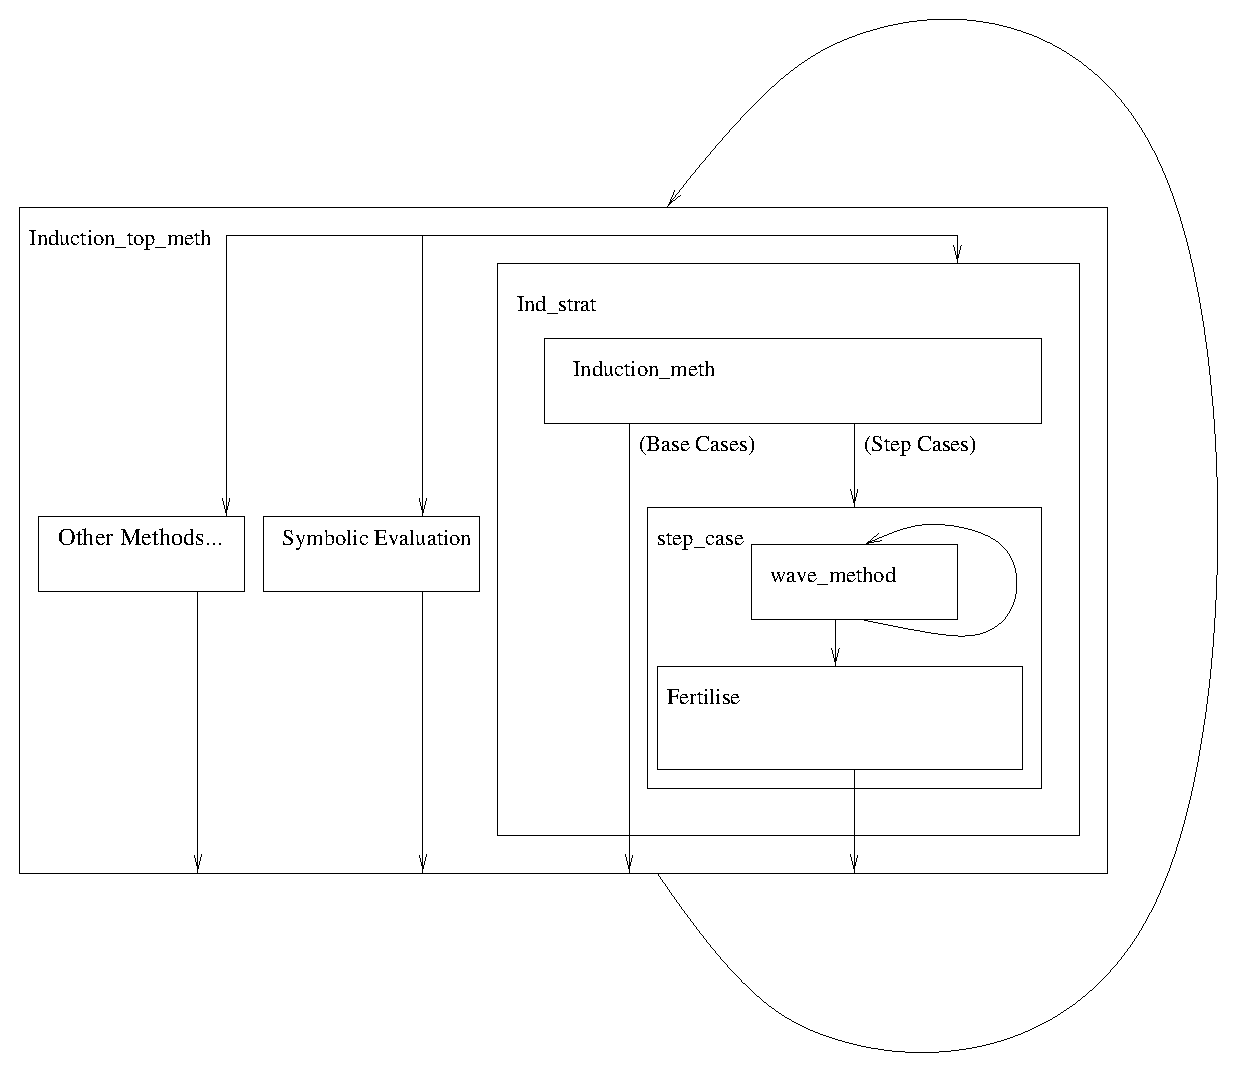
\epsfig{file=ind_strat.eps, width=4.8in}
\end{center}
\caption{The Proof Strategy for Induction}
\label{fig:induction_strategy}
\end{figure}
This is implemented as a selection of atomic and compound methods.
The diagram shows a top level repeat which attempts a disjunction of
methods.  These include basic tautology checking, generalisation of
common subterms and also symbolic
evaluation and the induction strategy ({\tt ind\_strat}).  Within the
induction strategy, the induction method
performs ripple
analysis~\cite{ind-chap-ref2} to choose an induction scheme (from a
selection specified in \lclam's theories) and produces subgoals for
base and step cases.  The base cases
are passed out to the repeat of the top level strategy.
The step cases are annotated with \emph{skeletons} and
\emph{embeddings} (described 
below) and then the wave method is repeatedly applied to them followed 
by fertilisation (exploitation of the induction hypothesis).
Annotations are then removed.  The methods ({\tt set\_up\_ripple} and
{\tt post\_ripple}) which place and remove annotations are omitted
from the diagram.  The results are then passed out to the top level
strategy again.  The process terminates when all subgoals have been
reduced to \emph{true} (or \emph{false} in the case of failure).

We will discuss the \method{wave\_method} in more detail since it was
a new formulation of this method we wished to investigate.  The wave
method embodies the rippling heuristic.  Rippling was first introduced
in~\cite{pub567}.  We use the theory as presented by Smaill \&
Green~\cite{pub799} who proposed a version that naturally coped with
higher-order features.  Rippling steps apply rewrite rules to a target
term which is associated with a skeleton and an embedding
that relates the skeleton to the target term (e.g.
rippling\index{rippling} rewrites an induction conclusion which has an
induction hypothesis embedded in it).  In the present context, we make
use of higher order rewriting, in the style of \cite{Fel92}.  After rewriting a new embedding of the skeleton into the rewritten term is calculated.  There is
a measure on embeddings and any rewriting step must reduce this
\emph{embedding measure} (written as $<_{\mu}$).  This is a
generalisation of the original version of rippling that used annotated
\emph{wave rules} to rewrite annotated terms.

Rippling is terminating~\cite{BasinWalsh96}.  Rippling either moves
differences outwards in the term structure so that they can be
cancelled away or inwards so that the differences surround a
universally quantified variable (or \emph{sink}).  If it is possible
to move differences inwards in this way the embedding is said to be
\emph{sinkable}.  The measure on embeddings allows differences that
are being moved outwards to be moved inwards but not vice versa --
this is at the heart of the guarantee of termination.

The \method{wave\_method} method has five preconditions.  It finds a
rewrite rule that rewrites the goal.  It then checks that there is
still an embedding of the skeleton into the rewritten goal and that
this new embedding is less, according to the embedding measure, than
the original embedding.  It checks that the embedding is sinkable and
that any conditions for the application rule are trivial.  This is
shown in figure~\ref{fig:wave_method}.  
%Sinkability is not necessary
%for termination but it is a useful further heuristic for guiding the
%proof.
\begin{figure}[htb]
\pageline
% \vspace{1mm}
\begin{center}
\begin{center}
\textbf{Input}

$$ripple\_goal(H \vdash G, S, E).$$
where $ripple\_goal$ is a triple of a sequent, a skeleton, $S$ and an
embedding, $E$, of that skeleton into the goal, $G$.
\end{center}
\begin{center}
\textbf{Preconditions}
\end{center}

\begin{enumerate}
\item The conditional
  rewrite rule \emph{Rule}, $Cond \imp X \rewrites Y$ instantiated
  with some substitution $\sigma$, applies to $G$
  and rewrites it to $G'$.
\item There is an embedding $E'$ that embeds $S$ in $G'$.
\item $E' <_{\mu} E$.
\item $\sigma(Cond) = True$ or $\sigma(Cond) \in H$.
\item $E'$ is sinkable.
\end{enumerate}
\begin{center}
\textbf{Output}
\end{center}
$ripple\_goal(H \vdash G', S, E')$
\end{center}
\vspace{1mm}
\pageline
\caption{The Wave Method}
\label{fig:wave_method}

\end{figure}
The method will backtrack\index{backtracking} in order to try to
satisfy all requirements, and if it is successful returns a new goal.

%The main advantages of rippling is that it allows an equation
%to be treated as a rewrite in both directions without loss of
%termination and provides useful information for automatically patching 
%failed proof attempts.  These abilities were not required in this case 
%studies and all the proofs went through automatically using 
%symbolic evaluation instead of rippling.  However, our intention was
%to test the higher-order presentation of rippling \emph{not} to justify 
%its necessity in the case of ordinals.

\section{Embeddings}
\label{embeddings}
We review here the notion of embeddings from Smaill \&
Green \cite{pub799}.  These provide the higher-order framework for
rippling used in this paper.

Embeddings are described by a tree data structure.  Embedding trees
describe how a \emph{skeleton} embeds in a term, called
the \emph{erasure}.  The nodes in an embedding tree
can be viewed as labels on the nodes in the term tree of the skeleton.
These labels contain addresses and directions.  The directions are
used during rippling as outlined above.  The addresses
are the addresses of nodes in the term tree of the erasure which
correspond to that node in the skeleton.  Term trees represent
function application and $\lambda$-abstraction explicitly as nodes with
constant and variables symbols appearing only at the leaves of the
tree.  Our implementation also contains tuple nodes for lists of
arguments to functions but these are not necessary to the theory.
Embeddings do not annotate $\lambda$-abstraction nodes.  Where an
embedding matches a variable in the skeleton to one in the erasure it
indicates that they are $\alpha$-convertible.
It is the ability to coherently handle
$\lambda$-abstractions which was particularly valuable in this
experiment.  The ability to handle difference occuring within functions as well
as the arguments to functions is also an extension of the previous
calculus.

\begin{example}
Consider embedding the term $\lam{x} f(x)$ into the term
$\lam{y} \lam{x} (f(y) + x)$. We 
do this as in figure~\ref{fig:embed}.  The two terms are shown 
as trees with branches represented by solid lines.  The address of
each node is given ($\lambda$-abstraction nodes do not carry
addresses).  The embedding appears
between them as an  
embedding tree with dashed lines -- the address label of
the nodes is 
also shown.  The dotted arrows illustrate how the embedding tree links 
the two terms.

\begin{figure}[htb]
\begin{center}
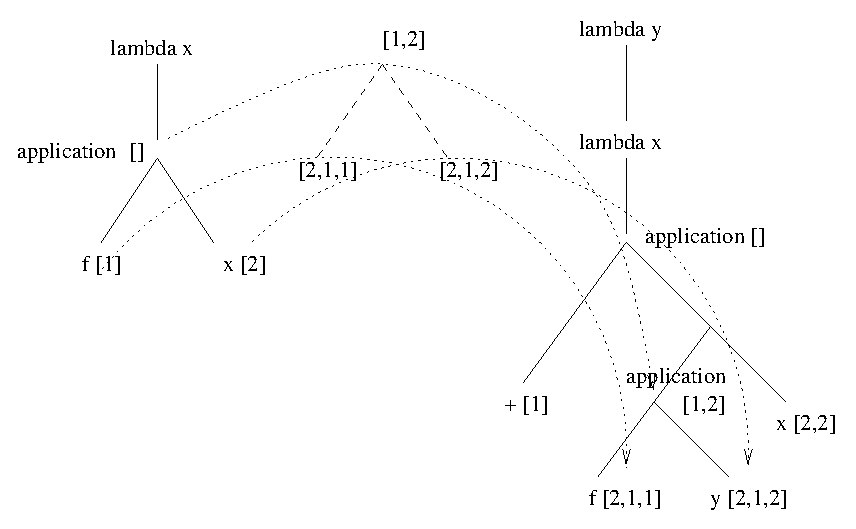
\epsfig{file=embed.eps, width=3in}
\end{center}
\caption{An Embedding}
\label{fig:embed}
\end{figure}

The embedding tree for this is  (node [1, 2] [(leaf
[1, 1, 1]) (leaf [2, 1, 2])])).  This states
that the function 
application at the top of $f(x)$ matches with the node at
address [1, 2] of $f(y) + x$ (i.e. the application involving $+$ has
been bypassed), that the
function symbol $f$ matches the sub term at [2,1,1] (i.e. $f$)
and $x$ matches $y$ (i.e.\ the bound variables can be consistently
renamed in either (or both) terms so that they are identical).

The annotations originally used in rippling 
are still useful for presentation.  Annotations consist of contexts
(expressions 
with holes) indicated by a wave front (box) with a directional arrow.
The holes in the context are wave holes (i.e. they are filled with an
expression which is underlined). The skeleton is everything
that appears outside wave fronts, or in wave holes. 
So the above embedding can be
presented as 
$$
\lam{x} \wfout{\lam{y} \wh{f(y)} + x}.
$$

NB.  It is important to remember that the annotations do not actually
exist in the implementation which records instead the 
skeleton and embedding\footnote{In fact \lclam\ maintains a list of
possible embeddings 
during rippling since there may be more than one way to embed the
induction hypotheses into the conclusion.  For convenience we assume
here there is only one.}.  
In some cases it is less easy to use the
traditional annotations to represent embeddings, particularly when dealing
with $\lambda$-abstrations which are ignored by the embedding trees.
You can see that in the above the bound variables in the skeleton 
are assumed to have been appropriately renamed already.
These 
annotations are just a presentational convenience.
\end{example}

\section{Logics}
You will note that the proof strategy for induction calls the {\tt
  taut}\index{taut} method for tautology checking.  This may vary
depending upon whether constructive or classical logic (for instance)
is being used.  As a result the basic ``build'' of the induction
theory\index{induction theory} in \lclam\ does not specify how the
{\tt taut} method or logical constants such as {\tt
  forall}\index{forall} or {\tt and}\index{and} should be treated by
the system.  It simply asserts that they exist.  Additional files, of
which the {\tt constructive\_logic}\index{constructive\_logic} theory
can then be created to provide the necessary details.

\section{Arithmetic, Natural Numbers and Lists}
There are a number of built-in theories dealing with natural number
and list theorems.  Standard functions and goals can be found in the
{\tt arithmetic}\index{arithmetic} theory and the {\tt
  objlists}\index{objlists} theory.  Further functions can be found in 
{\tt list\_benchmarks}\index{list\_benchmarks}, {\tt
  map\_benchmarks}\index{map\_benchmarks} and the {\tt
  clam\_corpus}\index{clam\_corpus} theories (there are 3 clam corpus
theory files).

\section{Mutual induction}
\noindent 
This module was written for the MFOTL group based at Liverpool.  The
method \texttt{alexei\_meth} in
\texttt{theories/mutual\_induction.mod} implements the following proof
rule.  It is a variant of a mutual induction rule suitable for
treatment of arithmetical translations of temporal formulae:

\vspace{0.5cm}

$ \forall y \forall \bar{x} A_{1}(y, \bar{x}) \Rightarrow B_{1}(s(y), \bar{x})$

$\forall y \forall \bar{x} A_{2}(y, \bar{x}) \Rightarrow B_{2}(s(y), \bar{x})$

$\ldots $

$\forall y \forall \bar{x} A_{n}(y, \bar{x}) \Rightarrow B_{n}(s(y), \bar{x})$

\vspace{-1mm}
$\underline{\qquad\qquad\qquad\qquad\qquad\qquad\qquad\qquad\qquad\qquad}$
 
\vspace{1mm}
$\forall u. u > t \Rightarrow \varphi(u)$ 

\vspace{5mm}
\noindent
with the side conditions: 

\[\begin{array}{l} 
\exists \bar{x}  (A_{1}(t,\bar{x}) \vee A_{2}(t, \bar{x}) \vee \ldots \vee 
A_{n}(t,\bar{x})) \\
\\
\forall y \forall \bar{x} (B_{i}(y, \bar{x}) \Rightarrow \varphi(y)) , i=1, \ldots, n \\
\\
\forall y \forall \bar{x} \exists \bar{z} ( B_{i}(y, \bar{x}) 
\Rightarrow \bigvee_{j=1\ldots n} A_{j}(y,\bar{z})) ,  i=1 \ldots, n 
\end{array}\]

\noindent
where $A_{i}$ and $B_{i}$ are arbitrary first-order formulae, $t$ is
an arbitrary arithmetical term, s is the successor function symbol,
$\Rightarrow$ is implication, $\bar{x}$ is a sequence of
variables, and $y$ is a (numerical) variable of type \texttt{nat}.  $n$ is
not fixed, so we can deal with arbitrary lists of premises in the rule.

\noindent
Since the rule is generally used in backward reasoning, 
one can present its application as follows: \\

\noindent
Given a goal sequent $H \vdash \psi$ with $\psi$ being of the form of
the conclusion of the above rule, the method generates some subset
$H'$ of $H$ matching the premises of the rule and generates the
associated side conditions as new subgoals.  These subgoals are
then resolved by application of some other methods (for first-order
reasoning). \\

\noindent
At present the method simply chooses the maximal matching subset of
hypotheses.  Probably some optimization for iteration over subsets
will be needed later.

\noindent{\bf Example:} \\

Given:   
\[\begin{array}{l}
\forall x, y (A(y,x) \Rightarrow B(s(y),x)) \\
\forall x, y (C(y,x) \Rightarrow D(s(y),x)) \\
\forall x (A(0,x) \lor C(0,x)) \\
\forall x,y (B(y,x) \Rightarrow C(y,x)) \\
\forall x,y (D(y,x) \Rightarrow (A(y,x) \lor C(y,x))) 
\end{array}\]

\vspace{-1mm}
$\underline{\qquad\qquad\qquad\qquad\qquad\qquad\qquad\qquad\qquad\qquad\qquad}$

Prove: 
\[\forall y > 0  \exists x (B(y,x) \lor D(y,x)) \]
 
Side conditions to prove (taking the set of first two hypotheses and the
conclusion):

\[\begin{array}{l}
\exists x (A(0,x) \lor C(0,x))\\
\\
\forall y \forall x (B(y,x) \Rightarrow  \exists z (B(y,z) \lor D(y,z))) \\
\\
\forall y \forall x (D(y,x) \Rightarrow  \exists z (B(y,z) \lor D(y,z))) \\
\\
\forall y \forall x \exists z (B(y,x) \Rightarrow A(y,z) \lor C(y,z)) \\
\\
\forall y \forall x \exists z (D(y,x) \Rightarrow A(y,z) \lor C(y,z)) \\
\end{array}\]
\newcommand{\lyacc}{$\lambda$yacc\xspace}

\chapter{Compiling Theories to \lclam}\label{compiler}

%\author{Ewen Denney}

\section{Introduction}

This chapter describes the current state of the \lclam theory
compiler.  It develops the idea that a logic can be presented in a
high-level declarative style, and then {\em compiled} down into a more
procedural implementation-specific language.

The reasons for wanting to do this are:
\begin{itemize}
\item the user-unfriendliness of the current \lclam format
\item to avoid errors that can arise when entering axioms and
  inferences as low-level rewrites and methods
\item (ultimately) to aim for a logic-independent planner by factoring out
  logic-specific code
\item since a high-level representation of logics and theories, rather than
  one which is hard-wired into a low-level implementation, is easier
  to communicate.
\end{itemize}

In our case, of course, the procedural language is \lclam's format for
the paraphernalia of proof planning (expressed in HOAS) in \lprolog;
for declarative language, we simply make up our own user-friendly
syntax for declarations, inference rules, and the like.


The compiler has two modes of use: online, using the {\tt add\_theory}
command during \lclam's normal command loop, and offline, generating a
separate \lclam theory file.  The offline mode is currently deprecated
but is described here as it helps understand the general compilation
process and may prove useful in the future.

\section{Online Mode}

The command
$${\tt add\_theory} \mbox{\em ``theory-file''}$$
will read in the file
{\em theory-file}, check its well-formedness, and generate the
appropriate user-defined constants.

For example, the file {\tt simpletheory}:
\begin{verbatim}
Theory Nsa.
Use Logic arithmetic.

type real.
type hyperreal.
$
\end{verbatim}
gives the following results:
\begin{verbatim}
lclam:
add_theory "simpletheory".
Trying ...Scanning for tokens...
Tokenizer stopped after line 6
Parsing...
Successfully parsed
Checking well-formedness...
Type real
Type hyperreal
Theory is well-formed
Importing lclam declarations...
Successfully processed
Done
Done
lclam:
\end{verbatim}
We can now use the query commands to check that the definitions have been made
correctly.
\begin{verbatim}
lclam:
query_osyn (user_theory "nsa") (user_object "real") X.
default
user_theory "nsa"
real
universe
lclam:
\end{verbatim}

A more complex example of a theory file can be seen in
Section~\ref{theory}.

\section{Offline Mode}

We describe here how a user can use the files {\tt
  envgrammar.\{sig,mod\}} and\linebreak 
{\tt postprocess.\{sig,mod\}} in the
{\tt compiler} directory to parse a theory file written in concrete
syntax and generate a \lclam theory file.

We first explain how to use the compiler, and in the following
sections, explain the workings of the compiler in case the user wants
to alter it.

The phases of such a logical compilation are much the same as in the
compilation of programs: parsing of concrete into abstract syntax
(Section \ref{parsing}), a well-formedness check (Section
\ref{well-formedness}), and then code generation (Section
\ref{generation}). We give the grammar for theory files (Section
\ref{grammar}), and examples of concrete syntax (Section \ref{theory}) and
the corresponding \lclam (Section \ref{lclam}).


\subsubsection{Using the Compiler}\label{makefile}

First, edit the {\tt Makefile}, if necessary, to alter the paths appropriately.

Then, generate the parser by
\begin{alltt}
make envparser
\end{alltt}
Next, do
\begin{alltt}
make postprocess
\end{alltt}

If the theory file is {\tt theoryfile}, then the command
\begin{alltt}
parsefile "theoryfile" X.
\end{alltt}
will bind to $\tt X$ the abstract syntax that results from parsing
this file. This might be useful to you if you just want access to the
higher-order abstract syntax form of an expression.

Here, {\tt theoryfile} is the file with concrete syntax which you can,
of course, change and rename. Note that the underlying parser, \lyacc,
requires this file to terminate with a {\tt \$}.

The command
\begin{alltt}
process_file "theoryfile"
\end{alltt}
will parse the file, check its well-formedness, and output the
appropriate \lclam files. The names of the files are determined by
the line
\begin{alltt}
Theory <name>.
\end{alltt}
in the theory file, which results in {\tt <name>theory.\{sig,mod\}}. 

Finally, you then have to fit these files in with your version of
lambda clam (by setting the appropriate accumulates) and compile the
whole system. Note that the compilation files themselves should not be
compiled with \lclam.


\subsection{Parsing}\label{parsing}

The logic file is first parsed into abstract syntax. The parser is
implemented using 
\lyacc\footnote{See {\tt http://www.cs.hofstra.edu/\~{ }cscccl/parsergen/.}}, 
a parser-generator written in \lprolog, due to Chuck Liang. It
generates bottom-up {\em shift-reduce} parsers, which can be less
intuitive than top-down parsers, but are more efficient.

The user specifies their logic by writing various predicates and rules
in a \lprolog file, which accumulates the \lyacc files.

\begin{enumerate}
\item Declare grammar symbols for the abstract syntax for each nonterminal.
\item Declare the terminals.
\item Give concrete syntax for the terminals using {\tt printname}.
\item List the terminals, and nonterminals.
\item Set {\tt ntnum} to the number of nonterminals plus 1.
\item
Give the parse rules, with semantic actions to construct
the abstract syntax.

For example, rules giving the syntax for axiom declarations are
\begin{verbatim}
 rule ((syn_decl_gs D5) ==> 
        [axiom_decl_gs S7 H1 Z7]) (D5 = axiom_decl S7 H1 Z7),

 rule ((axiom_decl_gs S5 H2 Z5) ==> 
        [axiomt, axiom_name I6, qprop_gs Z3, periodt]) 
                                (S5 = I6, Z5 = Z3, H2 = []),
\end{verbatim}
The {\tt rule} construct combines a production with a semantic action.
\item
Give precedence rules.
\item Supply freshcopy clauses for non-nullary nonterminals.
\end{enumerate}


This file is compiled, and then executed. Then, a generate parser
command is called, which, assuming \lyacc accepts the file, generates
{\em another} file. This file is then compiled to give the parser, all
of which takes about a minute in total.


\subsection{Well-formedness}\label{well-formedness}

A consequence of the fact that the semantic actions attached to \lyacc
parse rules cannot contain implications (and that \lprolog does not
have assertions), is that well-formedness of the resulting abstract
syntax has to be checked in a separate pass.

However, logically inspired manipulation of terms such as this is what
\lprolog does best.  For example, well-formedness of existentials and
abstractions is checked by
\begin{verbatim}
well_formed_assertion (app exists (tuple [T, abs P])) :-
        well_formed_type T,
        pi X \ (new_const X T) => well_formed_assertion (P (user_object X)). 

well_typed_term (ty_abs T L) (T arrow U) :-
        well_formed_type T,
        pi X \ (new_const X T) => well_typed_term (L (user_object X)) U.
\end{verbatim}
Since declarations are `first-class' in \lprolog, \lprolog's context
mechanism can be used for managing declarations.

\begin{verbatim}
well_formed_decls ((inference_decl S Hyps H2 C2)::Ds) :-
        well_formed_decl (inference_decl S Hyps H2 C2),
        ((new_inference S) => well_formed_decls Ds).

well_formed_decl (inference_decl S Hyps H2 C2) :-
        not (new_inference S),
        map_pred2 group_assertions Hyps Ass,
        all_pred well_formed_assertions Ass,
        ly_append H2 [C2] Ps2,
        well_formed_assertions Ps2,
        M is "Inference " ^ S ^ "\n",
        print M.
\end{verbatim}
There are no error messages at present.

\subsection{Generation of \lclam}\label{generation}
Once the theory file has been parsed into abstract syntax and checked
for well-formedness, it is converted to \lclam format and written to a
file. Constructing the appropriate higher-order abstract syntax was
done during parsing, so this stage is mainly concerned with
abstracting over the variables, and converting propositions to
rewrites and methods.

The syntax comprises a list of declarations, each of which is
converted to the corresponding \lclam entity.

\begin{alltt}
% decl2lclam {\it +sig-file +mod-file +theory-name +logic-name +declaration}

type decl2lclam  out_stream -> out_stream -> string -> string -> syn_decl -> o.
\end{alltt}
A syntactic declaration is one of: type, typed constant, axiom,
inference, conjecture, predicate symbol, definition.  The interesting
cases are axiom and inference rules. We convert axioms to rewrite
rules, and inferences to methods.

An example of an axiom is
\begin{verbatim}
axiom ax1 [y:nat |- forall f:nat->nat. f = (x:nat \ (f y))].
\end{verbatim}
This is parsed as
\begin{verbatim}
axiom_decl "ax1" (otype_of (user_object "y") nat :: nil) 
   (app forall (tuple ((nat arrow nat) :: 
         abs (W1\ app eq 
          (tuple (W1 :: ty_abs nat (W2\ app W1 (user_object "y")) :: nil))) ::
 nil)))
\end{verbatim}
and converted to the rewrite rule
\begin{verbatim}
axiom nsa ax11 ltor (trueP) 
   (app forall 
     (tuple ((nat arrow nat) :: 
       abs (W1\ app eq (tuple (W1 :: ty_abs nat (W2\ app W1 _107597) :: nil)))
 :: nil))) 
    (trueP).
\end{verbatim}


For inference rules, the system generates preconditions to check
for required antecedents in the conclusion, and to construct the
antecedents of the hypotheses. The succedent of the conclusion is
recorded in the form of the method input, and the succedents of the
hypotheses appear in the output goal.

For example, the inference rule
\begin{verbatim}
inference and_l [G,A,B,G' |- P / G, A /\B |- P]
\end{verbatim}
parses to abstract syntax
\begin{verbatim}
(inference_decl "and_l"
[(pair [user_object "G", user_object "A", user_object "B", user_object "G'"] 
       (user_object "P"))]
[user_object "G", (app and (tuple [user_object "A", user_object "B"])), 
user_object "G'"] (user_object "P"))
\end{verbatim}
which is converted to the atomic method
\begin{verbatim}
atomic nsa and_l
        (seqGoal (H >>> (_9055)))
        (sublist (app and (tuple (_9072 :: _9088 :: nil)) :: nil) H, 
        replace_in_hyps H (app and (tuple (_9072 :: _9088 :: nil))) 
                             (_9072 :: _9088 :: nil) H1)
        true
        seqGoal (H1 >>> _9055)
        notacticyet.
\end{verbatim}
The inference rule
\begin{verbatim}
inference and_r [G |- A ; G |- B / G |- A /\B]
\end{verbatim}
parses to abstract syntax
\begin{verbatim}
(inference_decl "and_r"
[(pair [user_object "G"] (user_object "A")),
(pair [user_object "G"] (user_object "B"))]
[user_object "G"] (app and (tuple [(user_object "A"), (user_object "B")]))
)
\end{verbatim}
and converts to
\begin{verbatim}
atomic nsa and_r
        (seqGoal (H >>> (app and (tuple (_5035 :: _5052 :: nil)))))
        (H =  H1, H =  H2)
        true
        seqGoal (H1 >>> _5035) ** seqGoal (H2 >>> _5052)
        notacticyet.
\end{verbatim}


\subsection{Theory Grammar}\label{grammar}

Identifiers can contain underscores but not hyphens. A theory begins
with a declaration of its name, and the logic it uses. The logic name
is not used, but must be entered for syntactic correctness.

\begin{verbatim}
Theory-declaration ::= 
        'Theory' Id '.'
        'Use Logic' Id '.'
        (Declaration '.')*

Declaration ::= Constant-declaration
                | Type-declaration
                | Axiom-declaration
                | Inference-declaration
                | Conjecture-declaration
                | Predicate-declaration
                | Definition


Constant-declaration ::= 'const' Id Type

Type-declaration ::= 'type' Id

Axiom-declaration ::= 'axiom' Id Prop | 'axiom' Id '[' Sequent ']' 

Inference-declaration ::= 'inference' Id '[' Sequents '/' Sequent ']'

Conjecture-declaration ::= 'conjecture' Id '[' Sequent ']'

Predicate-declaration ::= 'predicate' Id Type+

Definition ::= 'define' 'const' Id ':' Type '=' Term
             | 'define' 'type' Id '=' Type

Sequents ::= (Sequent ';')* Sequent

Sequent ::= Assumptions '|-' Prop

Assumptions ::= (Assumption ',')* Assumption

Assumption ::= Prop | Id ':' Type

Prop ::= 'forall' Id ':' Type '.' Prop
       | 'exists' Id ':' Type '.' Prop
       | Prop '/\' Prop
       | Prop '\/' Prop
       | Prop '=>' Prop
       | '<' Term '=' Term '>'
       | '(' Prop ')'
       | Id
       | Id '{' Term '}'

Type ::= nat | bool | '(' Type ')' | Type '->' Type | Type '#' Type | Id

Term ::= Id
       | (Id ':' type '\' Term ')'
       | '<' Term Term '>'
\end{verbatim}

\subsection{Theory file}\label{theory}
\begin{verbatim}
Theory Nsa.
Use Logic Thol.

type real.
type hyperreal.
const z nat.
const f nat->nat#bool.

axiom sch2 [x:nat |- <x=x>].
axiom sch3 [x:nat, y:nat |- <x=y>].
axiom sch4 [x:nat, y:nat, <x=y> |- <y=x>].
axiom ax1 [y:nat |- forall f:nat->nat. <f = (x:nat \ <f y>)>].
axiom exax exists x:nat. <x=x>.
axiom badax [true, x:nat |- <x=x>].

conjecture conj1 [x:nat |- forall y:nat . <x=y>].
inference inf1 [true |- false / true, x:nat |- <x=x>].

axiom qs (forall x:nat. (exists y:nat. <x=y>)) => true.

conjecture conj2 [x:hyperreal |- exists y:hyperreal . <x=y>].

predicate even : nat.
predicate close_to : hyperreal, real.

inference easy_inf [true|-true; false|-false / x:nat |- <x=x>].

axiom pred_in_prop even{z}.

define type real_pair = real#real.

define const n:nat#bool = <f z>.

define const m:nat = z.

axiom false_e [G1, false, G2 |- P].

inference and_r [G |- A; G |- B / G |- A /\ B].

inference and_l [G1,A,B,G2 |- P / G1, A /\B,G2 |- P].

inference or_l [G,A |- P; G,B |- P / G, A\/B |- P].
\end{verbatim}

\subsection{Generated \lclam}\label{lclam}
\begin{verbatim}
module nsatheory.

all_pred P nil.
all_pred P (H::T) :- P H, all_pred P T.
sublist Xs Ys :- all_pred (X\ (member X Ys)) Xs.

has_otype nsa real universe.
has_otype nsa hyperreal universe.
has_otype nsa z (nat).
has_otype nsa f (nat arrow tuple_type (nat :: bool :: nil)).
axiom nsa sch21 ltor (trueP) (_135695) (_135695).

axiom nsa sch22 ltor (trueP) (app eq (tuple (_137129 :: _137129 :: nil))) 
(trueP).

axiom nsa sch31 ltor (trueP) (_137732) (_137749).

axiom nsa sch41 ltor (app eq (tuple (_139400 :: _139383 :: nil))) (_139383) 
(_139400).

axiom nsa sch42 ltor (app eq (tuple (_144856 :: _144839 :: nil))) (app eq 
(tuple (_144839 :: _144856 :: nil))) (trueP).

axiom nsa ax11 ltor (trueP) (app forall (tuple ((nat arrow nat) :: abs (W1\ 
app eq (tuple (W1 :: ty_abs nat (W2\ app W1 _147505) :: nil))) :: nil))) 
(trueP).

axiom nsa exax1 ltor (trueP) (app exists (tuple (nat :: abs (W1\ app eq (tuple
 (W1 :: W1 :: nil))) :: nil))) (trueP).

axiom nsa badax1 ltor (trueP) (_148474) (_148474).

axiom nsa badax2 ltor (trueP) (app eq (tuple (_149926 :: _149926 :: nil))) 
(trueP).

top_goal nsa conj1 [(otype_of (user_object "x") nat)] (app forall (tuple (nat 
:: abs (W1\ app eq (tuple (user_object "x" :: W1 :: nil))) :: nil))).
atomic nsa inf1
        (seqGoal (H >>> (app eq (tuple (_152632 :: _152632 :: nil)))))
        (sublist (trueP :: otype_of (user_object "x") nat :: nil) H)
        true
        (seqGoal (H1 >>> falseP))
        notacticyet.

axiom nsa qs1 ltor (trueP) (trueP) (app forall (tuple (nat :: abs (W1\ app 
exists (tuple (nat :: abs (W2\ app eq (tuple (W1 :: W2 :: nil))) :: nil))) :: 
nil))).

axiom nsa qs2 ltor (trueP) (app imp (tuple (app forall (tuple (nat :: abs (W1\
 app exists (tuple (nat :: abs (W2\ app eq (tuple (W1 :: W2 :: nil))) :: 
nil))) :: nil)) :: trueP :: nil))) (trueP).

top_goal nsa conj2 [(otype_of (user_object "x") (user_object "hyperreal"))] 
(app exists (tuple (user_object "hyperreal" :: abs (W1\ app eq (tuple 
(user_object "x" :: W1 :: nil))) :: nil))).
atomic nsa easy_inf
        (seqGoal (H >>> (app eq (tuple (_156487 :: _156487 :: nil)))))
        (sublist (otype_of (user_object "x") nat :: nil) H, replace_in_hyps H 
(otype_of (user_object "x") nat) (falseP :: nil) H1, replace_in_hyps H 
(otype_of (user_object "x") nat) (trueP :: nil) H2)
        true
        (seqGoal (H1 >>> trueP) ** seqGoal (H2 >>> falseP))
        notacticyet.

axiom nsa pred_in_prop1 ltor (trueP) (app (user_object "even") (user_object 
"z")) (trueP).

definition nsa real_pair0 trueP (tuple_type (user_object "real" :: user_object
 "real" :: nil)) real_pair.
definition nsa n0 trueP (app (user_object "f") (user_object "z")) n.
definition nsa m0 trueP (user_object "z") m.
atomic nsa false_e
        (seqGoal (H >>> (_25170637)))
        (sublist (falseP :: nil) H)
        true
        trueGoal
        notacticyet.

atomic nsa and_r
        (seqGoal (H >>> (app and (tuple (_162845 :: _162862 :: nil)))))
        (true, H =  H1, H =  H2)
        true
        (seqGoal (H1 >>> _162845) ** seqGoal (H2 >>> _162862))
        notacticyet.

atomic nsa and_l
        (seqGoal (H >>> (_186518)))
        (sublist (app and (tuple (_186535 :: _186551 :: nil)) :: nil) H, 
replace_in_hyps H (app and (tuple (_186535 :: _186551 :: nil))) (_186567 :: 
_186535 :: _186551 :: _186583 :: nil) H1)
        true
        (seqGoal (H1 >>> _186518))
        notacticyet.

atomic nsa or_l
        (seqGoal (H >>> (_197214)))
        (sublist (app or (tuple (_197231 :: _197247 :: nil)) :: nil) H, 
replace_in_hyps H (app or (tuple (_197231 :: _197247 :: nil))) (_197247 :: 
nil) H1, replace_in_hyps H (app or (tuple (_197231 :: _197247 :: nil))) 
(_197231 :: nil) H2)
        true
        (seqGoal (H1 >>> _197214) ** seqGoal (H2 >>> _197214))
        notacticyet.

end

\end{verbatim}



%=========================
%%   Systemnamen
%%=========================

\newcommand{\Nat}{{\mathchoice{\displaystyle\rm I\hskip-0.21em N}%
{\textstyle\rm I\hskip-0.21em N}%
{\scriptstyle\rm I\hskip-0.14em N}%
{\scriptscriptstyle\rm I\hskip-0.14em N}}}
%%%%%%%%%%%%%%%%%%%%%%%%%%

\def\eps{\epsilon}
\def\name#1{#1}
\def\xspace{}
\def\activemath{{\it ActiveMath}}
\def\analytica{{\it Analytica}}
\def\automath{AUTOMATH}
\def\bliksem{{\it Bliksem}}
\def\chip{\mbox{CHIP}\xspace}
\def\chorus{Chorus}
\def\clamlite{{CLAM-Lite}}
\def\clos{{{\small CLOS}}}
\def\commonlisp{{{\footnotesize COMMON LISP}}}
\def\corba{{\sc Corba}}
\def\cosie{${\cal C}o{\cal SIE}$}

\def\davinci{\mbox{\sc daVinci}\xspace}
\def\declame{{{\small DECLAME}}}
\def\discount{{DISCOUNT}}
\def\doris{DORIS}
\def\eclipse{ECL$^i$PS$^e$}
\def\eqp{EQP}
\def\eprover{{\sf E}}

\def\fipa{{\sf FIPA}}
\def\fscos{${\cal FSC}o{\cal S}$}
\def\HOL{{$\cal HOL$}}
\def\hr{{\sf HR}}
\def\http{{\sf http}}

\def\ilf{{ILF}}
\def\ilog{ILOG}
\def\imply{IMPLY}
\def\imps{\mbox{\sc IMPS}\xspace}
\def\isabelle{\mbox{\it Isabelle}\xspace}

\def\keim{{\small\bf KEIM}}
\def\KEIM{{\small\bf KEIM}}
\def\kimba{{\sf Kimba}}
%\def\kqml{{\sc Kqml}}
\def\kqml{KQML}
\def\larks{LARKS}
\def\mathml{{\sc MathML}}
\def\oants{{\sf OANTS}}
\def\omrs{{\sc OMRS}}
\def\openmath{{\sc OpenMath}}
\def\omdoc{{OMDoc}} %\protect\omdocaux}
\def\omdocaux{\sc O\kern-1.6ex\raisebox{.4ex}{{\tiny M}}Doc}
\def\prosper{{\sc Prosper}}
\def\pvs{PVS}
\def\setheo{{SETHEO}}
\def\teamwork{{\sc Teamwork}}
\def\techs{{TECHS}}
\def\waldmeister{Waldmeister}
\def\xml{XML}
\def\xsl{{\sc Xsl}}

\def\lams{{\sf LaMS}}
\def\leo{\mbox{${\cal LEO}$}\xspace}
\def\lineq{{\sc LinEQ}}
\def\lisp{{\footnotesize LISP}}
%\def\loui{\mbox{{\sc L}$\Omega${\sc UI}}\xspace}
\def\LOUI{\mbox{\sc L}{\sc ovely} {$\Omega${\sc mega}} {\sc U}{\sc ser} {\sc I}{\sc nterface}}

\def\gap{GAP}
\def\cocoa{CoCoA}
\def\lba{LBA}
\def\lclam{\mbox{$\lambda$\--Clam}}
\def\mace{MACE}
\def\magma{{\sc MagMa}}
\def\maple{{\sc Maple}}
\def\mass{{\sc Mass}}
\def\mathematica{{\it Mathematica}}
\def\mathpert{{\it Mathpert}}
\def\mathweb{Math\-Web}
\def\mathwebsb{Math\-Web-SB}
\def\mathagent{\mbox{\sc MathAgent}\xspace}
\def\mbase{{\sc MBase}}
\def\mkrp{{MKRP}}
\def\mosh{\sc MoSh}
\def\mozart{\sc Mozart}
\def\multi{MULTI}
\def\mycas{\mbox{$\mu$\hspace{.2em}${\cal CAS}$}}
\def\MYCAS{\mbox{$\mu${\sc CAS}}}
\def\myCAS{\mbox{$\mu${\sc CAS}}}

\def\ND{{\small\bf ND}}
\def\nuprl{{Nuprl}}
\def\octopus{\mbox{$\Omega${\sc cTOpus}}\xspace}
\def\OMEGA{$\Omega${\sc mega}}
\def\omws{OMWS}
\def\otter{{\sc Otter}}
\def\oyster{{\mbox{\rm O\kern-.12em\raise.39ex\hbox{\sc y}\kern-.07emS\kern-.39em\raise.39ex\hbox{\sc t}\kern-.15em\hbox{\sc e}R}}}
\def\oz{{\sc Oz}}

\def\pds{PDS}
\def\POST{{\mbox{$\cal POST$}}}
\def\post{{\POST}}
\def\Post{{\POST}}
\def\prolog{PROLOG}
\def\lprolog{$\lambda$-PROLOG}
\def\protein{\mbox{\sc ProTeIn}\xspace}
\def\proverb{{\it PROVERB\/}}
\def\rdl{{\bf RDL}}
\def\sapper{{\sc sapper}}
\def\scetchpad{\mbox{SCETCHPAD}}
\def\solex{{\bf\sf SoleX}}
\def\spass{\mbox{\sc Spass}\xspace}
\def\strips{{\small STRIPS}}
\def\teyjus{Teyjus}
\def\tramp{{\sc TRAMP}}
\def\tps{TPS}
\def\tptp{{\sc TPTP}}
\def\tptptox{tptp2X}
\def\vampire{Vampire}
\def\weierstrass{{\it Weierstrass}}
\def\xmlrpc{XML-RPC}

%%\def\CLOS{{{\footnotesize COMMON LISP Object System}}}
\def\Omegapackage{{{\small\bf OMEGA}}}
%\def\clam{{\mbox{\rm CL\kern-.36em\raise.39ex\hbox{\sc a}\kern-.15emM}}}


\def\nd{{\bf ND}-Kalk"ul}
\def\lamcalc{\mbox{$\lambda$-Kalk"ul}}
\def\todo#1{{\sc #1}}
                                %\def\proverb{\mbox{\sc Proverb}\xspace}
                                %\def\clam{\mbox{\sc Clam}\xspace}
\def\hol{\mbox{\sc HOL}\xspace}
\def\nqthm{${\sc Nqthm}$}
                                %\def\tps{\mbox{\sc Tps}\xspace}
\def\clpr{\mbox{CLP(${\cal R}$)}\xspace}
\def\lmlb{\mbox{\sc LMLB}\xspace}
\def\LMLB{\mbox{\loui} {\sc M{\sc arkup}} {\sc L}{\sc anguage} {\sc B}{\sc rowser}}
\def\lml{\mbox{\sc LML}\xspace}
\def\LML{\mbox{\loui} {\sc M}{\sc arkup} {\sc L}{\sc anguage}}

\def\calculemus{\mbox{{\sc Calculemus}}}
\def\limplus{{\sc Lim-Plus}}
\def\limtimes{{\sc Lim-Times}}


\chapter{{\lclam} in the MathWeb Software Bus}\label{mathweb}

\author{J{\"u}rgen Zimmer}\footnote{The author was supported by the
  CALCULEMUS European Union IHP grant HPRN-CT-2000-00102.} (e-mail:
{\tt jzimmer@mathweb.org})\\
{\it This chapter summarises the work done by J{\"u}rgen Zimmer
  visiting the DREAM group as a CALCULEMUS Young Visiting Researcher
  (Oct. 2001 - Mar. 2002).}


\section{Introduction}
\label{sec:mw-intro}
The MathWeb Software Bus~\cite{FraKoh:mabdl99} is a platform for
distributed automated reasoning that supports the connection of a wide
range of mathematical services by a common software
bus.\footnote{Further information about the {\mathwebsb} is available
  at \url{http://www.mathweb.org/mathweb/}.}  The {\mathwebsb}
provides the functionality to turn existing reasoning systems into
mathematical services that are homogeneously integrated into a
networked proof development environment.  Client applications can
access 23 reasoning systems, for instance, the CASs {\maple},
{\magma}, and {\cocoa}, the constraint solver {\cosie}, mediators,
model generators, such as Mace and Satchmo, and the automated theory
formation system HR.  Moreover, the {\mathwebsb} integrates nine first
order ATPs, such as Otter, Spass and Bliksem, and E.
\begin{figure}[t]
 \begin{center}
   \epsfig{figure=mathweb-arch.eps,width=9cm}
   \caption{The MathWeb Software Bus}
   \label{fig:mathweb-arch}
 \end{center}
\end{figure}

The architecture of the MathWeb system is depicted in Fig.
\ref{fig:mathweb-arch}. Local {\em brokers} provide routing and
authentication information to the mathematical services. {\mathwebsb}
wrappers encapsulate the actual reasoning systems and offer the
mathematical services to their local broker.  Client applications such
as the {\OMEGA} system, HR, or {\lclam}, connect to a MathWeb broker
and request services.  In case the requested service is found, the
client application receives a reference to a newly created {\it
  service object}. The client can then send messages directly to this
service object.

\section{Integration of {\lclam}}
\label{sec:mw-integration}
We integrated {\lclam} into the {\mathwebsb} using the methodology
that has been successfully used for the integration of other systems
like the {\OMEGA} proof planner or the higher order theorem prover
{\tps}: A {\mathwebsb} {\it wrapper} implements the interface to the
services offered by {\lclam} and has full control over {\lclam} by
simulating user input using socket communication\footnote{Note: In the
  current implementation of Teyjus, socket communication only works on
  Solaris/SunOS machines.}. {\lclam} itself can use the wrapper to
access other services as external reasoning systems.

The implementation of {\lclam}, Teyjus {\lprolog}, does not allow
programming with multiple threads. Therefore, we had to define a new
interaction mode for {\lclam} in which the system reads commands from
the {\mathwebsb} socket:
\begin{description}
\item[{\tt sock\_read\_write}:] The top-level loop of a {\lclam}
  process in {\tt sock\_read\_write} mode exclusively reads commands
  from the {\tt lclam\_server\_socket}. The user cannot interact with
  the system via the usual toplevel loop.
%\item[{\tt sock\_interactive}:] I {\lclam} is running in {\tt
%    sock\_interactive} mode, the server socket is inactive. The {\tt
%    lclam\_client\_socket} can still be used to access external
%  reasoning systems in the {\mathwebsb}.
\end{description}

\subsection{Starting {\lclam} in the {\mathwebsb}}
To use {\lclam} within the {\mathwebsb} the system has to be
started by the {\lclam} {\mathweb} wrapper which establishes a socket
connection to the Teyjus process. This means, a {\mathwebsb}
installation is required.  At the moment, installing and configuring
the {\mathwebsb} is still a bit tricky. A detailed description of how
to install and configure the {\mathwebsb} can be found on the system's
homepage \url{http://www.mathweb.org/mathweb}. In the following we
only sketch the necessary steps to get an example session running on
DREAM machines:\\

\noindent Add the {\mozart} directory of the user {\tt jzimmer} to your path:
%\begin{itemize}
%\item {\tt cd \url{~}}
%\item {\tt ln -s /hame/jzimmer/.oz}
%\end{itemize}
%Expand your path to the Mozart directory:
\begin{itemize}
\item {\tt export  PATH=\$\{PATH\}:/hame/jzimmer/.oz/bin}
\end{itemize}
You can put this line in your \url{~/.bashrc} or your \url{~/.benv} file for the sake of convenience.

\noindent Copy {\mathwebsb}'s configuration files for the DREAM environment:
\begin{itemize}
\item {\tt cd \url{~}}
\item {\tt mkdir .mathweb}
\item {\tt cp -bi /hame/jzimmer/.mathweb/*config* .mathweb/}
\end{itemize}

The {\mathwebsb} expects that the environment variable
\url{LCLAM_HOME} is set to some installation of {\lclam} (Version 3.2.
or higher). If you don't have {\lclam} installed, please set the
variable to the installation of some other user, for instance, {\tt
  export LCLAM\_HOME=/hame/jzimmer/lclam}.  The same holds for the
variables {\tt TEYJUS\_HOME} which should point to the implementation
language {\teyjus}, and {\tt TJPATH} which defines the load-path of
{\teyjus} (cf.  section \ref{install}).
% instance:
%\begin{itemize}
%\item {\tt export TEYJUS\_HOME=/net/methven/disk/reason2/src/teyjus-test/juergen/teyjus-1.0-b30p2}
%\end{itemize}


\noindent Start the {\mathwebsb} and the {\lclam} system\footnote{Note that to be able to start
  {\tt lclam-mathweb} properly you should be a member of the user
  group {\tt dreamer}. Ask \url{gordon@dai.ed.ac.uk} for details.}  :
% {\mosh}\footnote{Further
%  information about the Mozart Shell (MoSh) can be found at
%  \url{http://www.mathweb.org/mathweb/mosh/}.} on methven or the host {\tt hostname}:
\begin{itemize}
\item {\tt lclam-mathweb}
\end{itemize}
An emacs window should appear with a {\lclam} process running in {\tt
  command\_pretty} mode. The system should behave like af ``normal''
{\lclam} except that the socket connection to the {\mathwebsb} wrapper
is established before the user is allowed to type in commands.  You
can try to plan a problem which uses the simplification of the
Computer Algebra System {\maple} during the planning process by typing
in the following commands:
\begin{alltt}
   add_theory_defs_to_sym_eval_list analytica.
   set_wave_rule_to_sym_eval.
   add_to_induction_scheme_list twostep2.
   pds_plan (induction_top normal_ind) fib_goal.
\end{alltt}
You should leave your {\lclam} system by typing {\tt halt.} in the
{\lclam} prompt and then {\tt C-x C-c} in the emacs window.


%Test {\lclam} with:
%\begin{itemize}
%\item {\tt testclam}
%\end{itemize}
%An emacs window should appear with a {\lclam} process running in {\tt
%  sock\_read\_write} mode.  After {\lclam} has finshed its search for
%a proof plan or after the time limit given by the test client is
%exceeded, the service is left again and the window should disappear.
%If the test worked fine, {\lclam} should be able to use all {\mathweb}
%services.

%To start an interactive {\lclam} session with an emacs interface, go
%to your {\mosh} and type
%\begin{itemize}
%\item {\tt lclam-mw}
%\end{itemize}
%The system should behave like af ``normal'' {\lclam} except that the
%socket connection to the {\mathwebsb} wrapper is established before
%the user is allowed to type in commands.


\section{{\lclam} using {\mathweb} Services}
\label{sec:mw-using-services}
For the use of external reasoning systems, we extended {\lclam} by the
modules \url{src/io/sockets.mod} and \url{src/plan/mathweb.mod} which
abstract from socket communication details and offers a convenient
interface to the {\mathwebsb} wrapper. The main predicates of the {\tt
  mathweb} module are the following:
\begin{description}
\item[{\tt mathweb\_get\_service}:]\ \\
  \hspace*{-1cm} {\small \tt string $\rightarrow$ string $\rightarrow$ o.}\\
  takes the service name as first argument (e.g.  "MAPLE", "OTTER")
  and returns a string uniquely identifying the service object in the
  second argument, if the service is available. If the service is not
  available, the predicate returns the string {\tt "error"}.
  
\item[{\tt mathweb\_apply}:]\ \\
  \hspace*{-1cm} {\small \tt string $\rightarrow$ string $\rightarrow$
    (list (list string)) $\rightarrow$ int $\rightarrow$ (list (list
    string)) $\rightarrow$ o.}\ \\ applies a method to a service
  object identified by the first argument. The second argument is the
  name of the service method. The third argument is a list of lists of
  strings representing the parameters for the method call. The fourth
  argument is an integer giving the timeout for the method call in
  seconds. The result of the method call is again encoded in a list of
  lists of strings and is unified with the fifth argument.
  
  The following example is taken from the module {\tt
    src/theories/maple.mod} and illustrates how to call the {\tt
    simplifyTerm} method of a {\maple} service:
  \begin{alltt}
mathweb_get_service "MAPLE" MapleService, 
print_open_math Formula OMFormula, 
OMObj is "'OMOBJ'(" ^ OMFormula ^ ")", 
mathweb_apply MapleService "simplifyTerm" [["1", OMObj]] 100 Result.
 \end{alltt} \vspace*{-0.4cm}
 First, a {\maple} service object is requested. Then a given {\tt
   Formula} is translated into {\openmath} representation. The
 {\openmath} object is given as the first (and only) argument to the
 {\tt simplifyTerm} service of {\maple}.
\item[{\tt mathweb\_leave\_service}:] \ \\
  {\small\tt  string -> o.}\\
  leaves the service object identified by the first argument. The
  service object and the corresponding reasoning system (e.g. a
  {\maple} process) is terminated. {\mathwebsb} clients should always
  leave service objects when they are no longer needed.
\end{description}


\noindent  We implemented the module
\url{src/io/print_open_math.mod} to translate {\lclam}'s formulae into
the {\openmath} standard using the core {\openmath} Content
Dictionaries (CDs). Thus, the module forms one half of an {\openmath}
phrase-book for {\lclam}. The translation table for {\lclam}'s symbols
is distributed over the theory files \url{src/theories/arithmetic},
\url{src/theories/analytica}, and
\url{src/theories/constructive_logic} to keep the {\openmath}
representation close to the definition of the symbols.


Using the {\tt mathweb} module, {\lclam} can now access every
reasoning system available in the {\mathwebsb}.  Possible applications
are:
\begin{description}
\item[Using ATPs to prove simple subgoals:] This approach has already
  been used in the {\OMEGA} proof planner to restrict the search
  space. In some cases, even higher order problems can be transformed
  to first order problems and then sent to one or more first order
  ATPs in the {\mathwebsb}.
%In {\OMEGA}, first order
%  resolution proofs are translated into natural deduction proofs by
%  the {\tramp} system.  This translation is not possible in {\lclam}
%  because in the current version {\lclam} does not have an associated
%  theorem prover with a logical calculus and tactics.
\item[Using ATPs on the control level:] It is a known shortcoming of
  {\lclam} that it does not check the consistency of hypotheses after
  performing a case split. This leads to {\lclam} missing easy proofs
  by inconsistency. Modern ATPs are very efficient and could detect
  trivial inconsistencies in a few milliseconds. We therefore try to
  prune inconsistent search paths in proof planning with the help of 
  ATPs like {\otter}.
\item[CAS computation in proof planning:] Due to our positive
  experience with CAS computations in many proof planning domains, we
  think that the use of CASs in inductive proof planning can enable
  {\lclam} to solve problems it couldn't solve before. The rewriting
  capabilities of a CAS can complement the rewriting of {\lclam} and
  can thus enhance the reasoning capabilities of {\lclam}.
\end{description}

Until now, we focused on the latter and formalised problems taken from
the {\analytica} system~\cite{Clarke92-1,BaClZh:aectpsc98} and the
{\clamlite} system~\cite{Walsh00}\footnote{NOTE: Due to a bug in
  {\teyjus}'s memory management, most of the examples do not run with
  {\teyjus} Version 1.0-b30p2.}. The {\analytica} problems can be
found in the theory file \url{src/theories/analytica.mod} and the
summation problems in the file \url{src/theories/sums.mod}.  During
the planning for these problems, {\lclam} uses {\maple}'s {\tt
  simplifyTerm} service which gets a term (formula) in {\openmath}
representation as an input argument. It returns the {\openmath}
representation of the term (formula) resulting from the call of
{\maple}'s {\tt simplify} function.  For the access of {\maple}, we
defined the {\tt maple\_simplify\_meth} which calls the {\tt
  simplifyTerm} service of {\maple} on the current subgoal and
introduces the resulting formula as a new subgoal. The method is
defined in the module \url{src/theories/maple.mod}. It should fail if
{\lclam} is in standalone mode and no {\mathwebsb} connection can be
established.  We added {\tt maple\_simplify\_meth} to the compound
methods {\tt induction\_top} and {\tt fertilise} defined in the module
{\tt src/theories/induction.mod}.


\section{Services offered by {\lclam}}
All services offered by {\lclam} are based on the
{\openmath}~\cite{CapCoh:doms98} and the
{\omdoc}~\cite{Kohlhase:otormd00} standard. We implemented a
translation service (the second half of a phrase-book) to translate
incoming formulae, definitions, and conjectures into {\lclam}'s higher
order abstract syntax. For the sake of efficiency, this translation is
performed by the {\mathwebsb} wrapper.  {\lclam} currently offers two
services to the {\mathwebsb}:
\begin{description}

%       meth planProblem(Conjecture  ?Result
%                        method: Method   <= "(induction_top with_critics)"
%                        timeout: TimeOut <= 60 )
  
\item[{\tt planProblem:}] This service takes an {\omdoc} document,
  containing a single conjecture, as an argument. The service starts
  the {\lclam} proof planning mechanism on the conjecture. In our
  current implementation, the service expects the conjecture to be
  about natural number arithmetic. We plan an extension of the service
  such that clients can also provide the theory the conjecture is
  defined in.
  
  Client applications using the {\tt planProblem} service can use
  optional arguments to determine which proof strategy (compound
  method) {\lclam} should use for the planning attempt, and to give a
  time limit in seconds.  In the current implementation, the service
  simply returns the {\openmath} symbol $true$ if {\lclam} could find
  a proof plan within the given time limit, and $false$ if no proof
  plan could be found.
%In section \ref{sec:concl}, we describe
%  possible future extensions of the {\tt planProblem} service.
  
\item[{\tt ripple:}] Rippling is one of the most successful heuristics
  for guiding (inductive) proof planning. Therefore, {\lclam} offers
  its rippling mechanism as a separate service to the {\mathwebsb}.
  The service is given a single {\omdoc} document as an input. The
  {\omdoc} must contain a non-empty set of rewrite rules, formalised
  as lemmas, and a goal sequent $H\vdash \phi$ as a conjecture. The
  {\tt ripple} service tries to reduce the difference between $\phi$
  and the best suitable hypothesis in $H$ using the rewrite rules.
%\ednote{ld: Is
%    this right? Or does it reduce w.r.t.. all hyps?}.
% The rewrite rules
%  must be specified separately using the {\tt setRewriteRules}
%  service.\ednote{jz: We could actually put the two services together
%    in one. This would of course mean that we lose the context after
%    every call.}
  The {\tt ripple} service also tries to apply fertilisation to reduce
  the goal $\phi$ to the trivial goal $true$.  The service returns the
  {\openmath} symbol $true$ if this was successful and $false$
  otherwise.  In a future version, the {\tt ripple} service should us
  the partial planner, implemented by Louise Dennis, to ripple as far
  as possible and return an {\omdoc} which contains the resulting
  proof planning goal as a sequent $H\vdash \phi'$.
    
%\item[{\tt setRewriteRules:}] is used to tell {\lclam} which set of rewrite
%\item[{\tt setRewriteRules:}] is used to tell {\lclam} which set of rewrite
%  rules it should use for the next {\tt ripple}. The rewrite rules should be
%  provided as definitions or lemmas in {\omdoc} format, i.e. as a single
%  {\omdoc} document containing a list of assertion elements.\ednote{jz: maybe we
%    should show an example in a figure. Anyway we should at least show one
%    {\openmath} formula somewhere. Makes a good impression.}. Using the {\tt
%    setRewriteRules} service, a client application can set up an simple {\it
%    context} such that it does not have to send the rewrites again and again
%  for every call of {\tt ripple}. \footnote{There is still a lot of conceptual
%    work to be done on the notion of {\it context} in communication between
%    reasoning systems and this is just a first step.}

\end{description}
%The {\mathwebwrapper also forwards {\mathwebsb} service calls performed by
%{\lclam}.
The services offered by {\lclam} can be used by other reasoning
systems via the {\mathwebsb}. We made first experiments with the use
of the {\tt planProblem} service and the {\tt ripple} service within
the {\OMEGA} proof planner.  We formalised problems in the natural
number theory of {\OMEGA} and implemented proof planning methods that
call the {\tt planProblem} and the {\tt ripple} service of {\lclam} to
close open subgoals or to reduce a subgoal to a simpler one,
respectively.

To see {\OMEGA} calling {\lclam}'s services, do the following:\\
Start an omega by typing in a shell:
\begin{itemize}
\item \url{loui-local}
\end{itemize}
A window with the GUI of {\OMEGA} should appear. Read in a problem and plan it:
\begin{itemize}
\item choose the menu  {\tt File}$\rightarrow${\tt Read}$\rightarrow${\tt Problem}
\item Click {\tt Choose File...}
\item choose {\tt /hame/jzimmer/xmp/plus2right.post}
\item execute one planning step with the menu {\tt
    Planner}$\rightarrow${\tt Step Plan} or with {\tt CTRL+t}.
\end{itemize}
During the planning step, the {\OMEGA} proof planner tries to apply
methods for the call of both the {\tt ripple} and the {\tt
  planProblem} service. This is why you see two windows of {\lclam}
services popping up on the screen. In our example only the {\tt
  planProblem} leads to success and the proof planning goal in
{\OMEGA} is closed with the justification {\tt LCLAM-M}, i.e. the
proof planning method that called {\lclam}'s {\tt planProblem}
service. You can also see a window with title "Oz Browser" which shows
the lemmas {\OMEGA} sends to {\lclam} for the rippling\footnote{Change
  the representation mode in the Browser menu "Options" to see show
  strings and virtual strings strings properly. Then select the whole
  Browser output and type {\tt C-b}. Further information can be found
  at \url{http://www.mozart-oz.org/documentation/browser}.}.

%One advantage of passing lemmas from {\OMEGA}'s theories as rewrites
%to {\lclam}'s {\tt ripple} service is that the rewriting process is
%completely independent of {\lclam}'s theories. Thus, {\lclam} can be
%used as an abstract rewriting engine whose termination is guaranteed.
%However, the current version of {\lclam} does not maintain a trace of
%the positions of subterms a rewrite rules was applied to. The latter
%would allow the {\tt ripple} service to tell a client application, like
%{\OMEGA}, exactly which rewrite has been applied to which subterm of
%the planning goal not just the rewrite rule that had been applied to
%that goal. {\OMEGA} could then use this information to construct a
%natural deduction proof for the reasoning steps performed during
%rippling.


%%============================================
%% Future Work
%%============================================
\section{Possible Future Work} 
\label{sec:future}
% \begin{itemize}
% \item more context and interaction in service calls
% \item decision procedures in {\mathwebsb}
% \item use of {\mbase} as mediator
% \end{itemize}
%The preliminary results we got from our experiments with the use of
%CAS in inductive proof planning were promising and in the future one
%could extend our experiments to a fully-fledged case study by
%formalising all theorems about closed forms of summations listed
%in~\cite{TobyMaple}. We plan a more detailed comparison of our work
%with~\cite{TobyMaple} on the basis of qualitative results (the number
%of proof plans found) and on quantitative results (runtime
%comparisons).
Possible directions for future work include the use of other external
reasoning systems such as ATPs or decision procedures in {\lclam} as
described in section \ref{sec:mw-using-services}.

Our experiments with the use of Computer Algebra computations in proof
planning could be extended to a full case study. Especially the
summation problems of \cite{Walsh00} are interesting for this application.

The services offered by {\lclam} could be refined and extended. The
{\tt ripple} service, for instance, should return the subgoal after
one application of the rippling method (and fertilisation). The
service could also return the list of rewrite rules applied, and the
positions of the subterms the rules were applied on.  The {\tt
  planProblem} service could be extended to take the definition of the
theory a problem is formulated in, and to return a (partial) proof
plan in {\omdoc} encoding.

Furthermore, {\lclam} offers the means to formalise and prove theorems
in non-standard analysis (NSA)~\cite{Maclean02}. Using NSA, {\lclam}
could already find proof plans for the limit theorems {\limplus} and
{\limtimes} and some other analysis theorems, e.g., the mean-value
theorem. In contrast to the classical $\eps$-$\delta$ proofs, NSA
proofs tend to be much shorter and more intuitive.  Hence, it would be
interesting to use {\lclam}'s NSA theory to construct alternative
proofs for some of the complex theorems proved by the {\analytica}
system using the computational power of CASs available in the
{\mathwebsb}.

% Significant work has been done by \name{P. Jani\v{c}i\'c} on the
% integration of different decision procedures to produce more powerful
% ones~\cite{Janicic01} using a proof planning framework.  Decision
% procedures are of general interest for any reasoning system,
% especially for DSs, because they provide efficient algorithms to solve
% subproblems in a decidable theory.  We therefore intend to integrate
% decision procedures in the {\mathwebsb} and define a reasoning service
% common to all decision procedures. {\lclam} could then use the
% {\mathwebsb} for a homogeneous, distributed access of various decision
% procedures.

% \ednote{ld: not sure how all this fits together, it doesn't
%   make much sense to me.  The framework for constructing decision
%   procedures is implemented in \lclam\ although I think Predrag wanted
%   to call external reasoners on occasion but he was using methodicals
%   to string them together}
 
The proper use of context in the communication between reasoning
systems is still an open research question. Context can not only
reduce the amount of information that has to be transfered between
systems, it is also crucial to establish more complex forms of
collaboration and coordination between reasoning systems. The {\lclam}
proof planner, for instance, offers the powerful {\it critics}
mechanism which analyses the failure of a proof attempt and gives
feedback to the user about possible ways of correcting the proof.
This feedback can include generalising the original goal, modifying
the chosen induction scheme, or speculating a new rewrite rule.
Potentially this feedback could also be given to another reasoning
system using {\lclam} and this would involve far more complex
interactions in terms of context.  For instance, if {\lclam} were to
suggest modifying the induction scheme this new proposed scheme might
have to be transmitted back to the client system for verification in
terms of its own logic. To enable this form of fine-grained
interaction between reasoning systems we need to develop a general
notion of context in inter-system communication.  {\lclam} could then
be used as a prototypical reasoning systems that builds up a context
when communicating with other systems.
 





%%% Local Variables: 
%%% mode: latex
%%% TeX-master: "manual"
%%% End: 

\chapter{Developing \lclam\ }
\label{developer}

\section{Introduction}
This chapter is intended mainly for the primary developer(s) of
\lclam\ .  It contains information on the system architecture of the
current version (v4.0.0) of \lclam\ , an discussion of the core
planning modules, an overview of the contents of the theory library,
and lastly some information on benchmarking.

This chapter may seem a little disjointed , having been written by two
different developers at different times.  In particular, section 10.2
on the \lclam\ architecture was written by James Brotherston (Aug 2001
-- Oct 2002); the rest is mostly due to Louise Dennis (Aug 1999 -- Aug
2001) but has been updated.

\section{\lclam v4 schematics}

\subsection{The Teyjus module system}

It is important to understand the meanings of the various types of arc
in the schematic diagrams we present, since they correspond to rather
different types of module accumulation in Teyjus.

Dotted lines correspond to \emph{signature extension}.  In other
words, if there is a dotted arc from M2 upwards to M1, then in the
signature of M1 we have {\tt accum\_sig M2.}  Thus all the predicates
and constants declared in the signature of M2 are ``pasted'' into the
signature of M1, and therefore are visible to other modules that accumulate
M1.  However, the actual predicate definitions in M2 (if any) are
\emph{not} accumulated into M1.  This may seem strange, but in most
cases we do this to avoid the situation where the same predicate
definitions are accumulated more than once into a higher-level module.
In that situation, those predicates start to succeed once for each
copy of the definition accumulated --- which is not desirable.  We
therefore import the signature only, in order to avoid type errors,
and make sure that the code for each module is accumulated only once.

Solid lines correspond to \emph{global accumulation} of modules --- if
there is a solid line upwards from M2 to M1, then in the body of M1 we
have {\tt accumulate M2} and in the signature of M1 we have
{\tt accum\_sig M2}.  So in this case, as with signature extension, all
the declarations in the signature of M2 are visible in M1 and outwards
from it, but the predicate definitions of M2 are now also present in
M1 and visible outwards from it.

Lastly, dashed lines correspond to \emph{local accumulation} of
modules, with the possibility of partial outwards visibility.  If
there is a dashed line upwards from M2 to M1 then in the body of M1 we
have both {\tt accumulate M2} and {\tt accum\_sig M2}.  No mention of
M2 is made in the \emph{signature} of M1, however.  Doing this treats
all the declarations and definitions in M2 as local to M1, and thus
not visible to modules that accumulate M1.  However, we can allow a
part of the signature of M2 to percolate outwards by repeating the
relevant part of M2's signature in the signature of M1.  Then those
declarations and any associated predicate definitions are visible to
modules that accumulate M1.  Local accumulation is thus useful when we
wish to conceal module code from higher-level modules.

We now proceed to present the schematics for \lclam v4, along with
brief descriptions of the component modules.

\subsection{Syntax and utilties (Fig. 1)}

\begin{figure}
\begin{center}
\epsffile{lclamv4_syntax.eps}
\end{center}
\caption{\lclam\ syntax declarations and utility functions}
\end{figure}

\begin{description}
  
\item[lclam\_list] All the usual list utilities including member,
  append and so on.
\item[lclam\_map] Map utility predicates.
\item[lclam\_utils] Utility supermodule which includes the list and
  map predicates, plus miscellaneous utilities such as findall.
\item[basic\_types] Declarations for the most fundamental types in
  \lclam\ such as methods, goals, plan states and so on.
\item[rewrite\_types] Declarations for types and predicates used in rewriting.
\item[ripple\_types] Declarations for types and predicates used to support rippling.
\item[method] Basic method predicates atomic and compound, plus
  declarations for the various methodicals.
\item[goal] Declarations for the various goal constructors, plus a
  couple of utility functions on goals.
\item[syntax] Declarations for the constructors of osyn, which is the
  metalanguage used for goals in \lclam, plus utility functions for
  typechecking etc.
\item[plan] Constructors for plan states plus utility functions on plans.  
\item[critics] Basic critics plus declarations for the criticals.
\item[lclam\_syntax] Syntax / utility supermodule which includes all
  of the modules above, plus predicates for querying the various
  rewrite rule lists.
\end{description}

\subsection{Pretty printer (Fig. 2)}

\begin{figure}
\begin{center}
\epsffile{lclamv4_printer.eps}
\end{center}
\caption{The \lclam\ pretty printer}
\end{figure}

\begin{description}
  
\item[pretty\_print] Declarations for the pretty-printing markup
  syntax, plus predicates for pretty-printing primitives.
\item[prettify] Predicates for marking up various syntax expressions for the pretty printer.
\item[interaction] Various output mode switches for controlling how an expression is printed.
\item[print\_syntax] Predicates for pretty-printing terms, goals, methods etc.
\item[print\_open\_math] Predicates for pretty-printing OpenMath terms.
\item[print\_plan] Predicates for pretty-printing plans.
\item[pretty\_printer] Interface for the pretty-printer.  Notice that
  the other pretty-printing modules are locally accumulated into this
  module, allowing careful control over which printing predicates are
  visible to higher modules.
\end{description}

\subsection{Planner core (Fig. 3)}

\begin{figure}
\begin{center}
\epsffile{lclamv4_planner.eps}
\end{center}
\caption{The \lclam\ planner core}
\end{figure}

\begin{description}

\item[switch] Declarations for various switches which affect planner operation.
\item[plan\_support] Predicates for manipulating the agenda and for
  tidying method continuations.
\item[pds\_support] Most of the important planning predicates are in
  this module, including the predicates for applying methods and
  critics, and for transforming compound methods into a first method
  and continuation.
\item[pds\_planner] Main predicates for the Partial Data Structure planner, in depth-first and iterative deepening flavours.
\item[part\_plan] Main predicates for a partial planner.
\item[planner] Planner interface, including wrappers for calling the
  various planners.  The actual code for the syntax and pretty-printer
  supermodules is accumulated into this module.  Notice that the other
  planner modules are accumulated locally, ensuring that the planners
  can only be called via the interface provided by this module.
\end{description}

\subsection{Core theories (Fig. 4)}

\begin{figure}
\begin{center}
\epsffile{lclamv4_theories.eps}
\end{center}
\caption{The \lclam\ theory core}
\end{figure}

\begin{description}
  
\item[logic\_eq\_constants] Declarations for logic constants and
  logical methods needed for the higher core theories.
\item[pairs] Declaration and syntactic sugar for pairing type.
\item[generalise] Generalisation method and supporting predicates.
\item[embed] Support for embeddings.
\item[rewriting] Generic rewriting methods and supporting predicates.
\item[casesplit] Support for case-splitting.
\item[wave] Support for rippling, including atomic wave methods.
\item[schemes] Support for induction schemes, including ripple analysis.
\item[induction] Methods for induction and supporting predicates.
\item[wave\_critics] Supermodule for the core theories of \lclam\ with
  the usual control over the interface in order to hide the internal
  supporting predicates.
\end{description}

\subsection{Top-level interface (Fig. 5)}

\begin{figure}
\begin{center}
\epsffile{lclamv4_top.eps}
\caption{The top level of \lclam}
\end{center}
\end{figure}

\begin{description}

\item[theory\_db] Predicates for querying the \lclam\ theory database.
\item[lclam] Top-level module which accumulates the theory core and
  the planner and contains all of the various user commands.

\end{description}




\section{The Proof Planning Core}
This section goes through the files in the core proof planning making
notes on anything of interest in those files.  Much of the following
will make little sense unless you have the code to hand to refer to.

\subsection{Planner}
The ``top'' module of the core proof planner is {\tt planner.mod}/{\tt
  planner.sig}\index{planner.mod}\index{planner.sig}.  The planner is
supposed to provide a generic top level predicate for applying any
proof planner built into the system to any goal --- which is what {\tt
  plan\_this}\index{plan\_this} does.  So {\tt plan\_this} takes as
arguments a proof planner predicate\index{proof planner predicate}, a
method\index{method}, a goal\index{query} and what is called an {\em
  agenda predicate}\index{agenda predicate} which is supposed to
define a search strategy\index{search strategy}.  The idea is that
{\tt plan\_this} applies the proof planner to the given goal using the
given method and search strategy.  In practice \lclam\ has two proof
planners; the PDS planner (in {\tt pds\_planner.mod}, in iterative
deepening and ``Claudio'' varieties), and a partial planner (in {\tt
  part\_plan.mod}), and only one agenda strategy which is the
depth-first\index{depth first} strategy.  (However, it should be no
problem to code up other stratgeies if required.)  In order to speed
up and facilitate use of the system we have wrappers for the various
planners in {\tt planner.mod} which call {\tt plan\_this} with the
appropriate planner and strategy.

\begin{verbatim}
plan_this Proof_planner Method Query AgendaPredicate:-
        top_goal _ Query  Hyps Osyn, !,
        announce_start Query Osyn,
        Proof_planner (pstate (active_agenda [nil]) 
          (and_node (seqGoal (Hyps >>> Osyn))
                     nil
                     open_status
                     Method
                     nomethodyet
                     []
                     []
                     notacticyet
                     []))
          AgendaPredicate
          Plan, !,
        ((Plan = (pstate _ VerbosePlan), !, pprint_plan VerbosePlan);
        (Plan = (cpstate _ CPlan), pprint_cplan CPlan)),
        announce_end, !.
\end{verbatim}
{\tt announce\_start}\index{announce\_start} and {\tt
  announce\_end}\index{announce\_end} just print out information at
the start and end of planning.  {\tt top\_goal}\index{top\_goal}
retrieves the actual sequent ({\tt Osyn}) which must be proved.  The
proof planner {\tt Proof\_planner} to an empty agenda {\tt (pstate
  (active\_agenda [nil]))}\index{pstate}\index{active\_agenda}, an
initial {\tt and\_node}\index{and\_node} of a plan (notice this has
lots of empty slots because nothing has happened yet), and the agenda
predicate\index{agenda predicate}, getting back a {\tt Plan} as
output.  There is then a disjunction on how the plan should be
treated.  If the plan is a {\tt pstate}\index{pstate} then it is
verbose (i.e. it contains all the plan information) otherwise it has
been stripped down and contains just method and goal information ({\tt
  cpstate}\index{cpstate}).  This is because full plans were difficult
to read and took up too much memory.  (Hopefully somebody will
implement some decent pretty printing for plans soon).

\subsection{pds\_planner}
So what does the PDS planner\index{PDS planner} actually do?  The
predicate {\tt pds\_planner} actually just passes everything on to
{\tt context\_planner}\index{context\_planner} adding an {\em
  action}\index{action} and asserting the first node in the plan ({\tt
  pplan\_node}\index{pplan\_node}).

The heart of this planner is the clause
\begin{verbatim}
context_planner ActionIn Agenda AgendaPredicate PSOut:-
        context_plan_step ActionIn ActionOut Agenda AgendaOut NewNodes,
        %% AgendaOut is containd in ActionOut
        create_agenda ActionOut (pliststate AgendaOut NewNodes) 
                AgendaPredicate (pliststate NewAgenda NewNewNodes),
        context_planner_nodes ActionOut NewNewNodes NewAgenda AgendaPredicate PSOut.
\end{verbatim}
The predicate {\tt context\_plan\_step}\index{context\_plan\_step}
performs one planning step.  This takes the current
agenda\index{agenda} and action\index{action} and applies the action
appropriately to the agenda (the action tells the planner whether to
apply a method or a critic) and returns a new action and agenda as a
result.  The reason the {\tt context\_plan\_step} predicate can alter
the agenda is in the case of critics\index{critic} etc. where it may
want to delete nodes from the agenda.  It also returns a list of the
nodes in the plan that have been altered as a result of the action.
{\tt create\_agenda}\index{create\_agenda} uses the new agenda, the
list of changed nodes and the agenda predicate to create a further new
agenda.  For example, in depth-first planning\index{depth-first} it
would put any new nodes on the front of the agenda while in
breadth-first planning it would put them at the end.  Note that this
just handles the order in which subgoals are treated.  There is also a
question about handling different outcomes for method application on a
given subgoal.  The planner then recurses.  There are extra clauses in
{\tt context\_plan\_step} apart from the base case.  These are
attempts to deal with cuts which have never worked satisfactorily.

This planner (and its name) require some explanation.  The first pass
at implementing a partial data structure planner\index{pds planner} in
Teyjus resulted in an algorithm that was immensely space
hungry\index{memory}.  The planner failed to find plans for the
associativity of append\index{associativity of append}, exceeding of
the simulator's allowed heap size\index{heap size} of 120 Megabytes.

While the memory\index{memory} needed by the planner was not so large
or so catastrophic in the Mali version of \lclam, it was of concern.
Jeremy Gow had processes that were taking up as much as a gigabyte and
there were a couple of theorems we were failing to plan for supposed
space reasons (though this was never satisfactorily proved).

An alternative way of communicating plan information within the
program has been devised which seems to have substantially solved the
space problems in \lclam.

\noindent {\bf \lprolog's {\tt =>} Symbol\index{{\tt =>}}} \\

\lprolog\ does not contain the {\tt assert}\index{assert} and {\tt
  retract}\index{retract} predicates which allowed Prolog programmers
to essentially modify the predicates (and hence data) of their program
dynamically at run time.  Instead \lprolog\ achieves this using {\tt
  =>}\index{{\tt =>}}, which has roughly the same semantics as
implication.  Below a simplified section of \lclam's top level loop is
shown.  {\tt lclam}\index{lclam} is the predicate that controls the
loop.  It waits for an input from the user and then executes the
command they have given.  In this case the user has specified that a
new piece of syntax is to be used in future proof attempts.  \lclam\ is
most interested in the type of syntax (especially in the
generalisation method) and refers to a predicate {\tt
  has\_otype}\index{has\_otype} when it needs to use this.  The code
fragment below shows what happens when the user wants to dynamically
add a piece of syntax.  Essentially the program just returns to the
{\tt lclam} loop, but this time there is an extra clause of {\tt
  has\_otype} added using {\tt =>}.

\begin{verbatim}
execute_command (add_osyn Syntax Type):-
        (has_otype Syntax Type) => lclam.
\end{verbatim}\index{execute\_command}

The scope of this implication is the right hand side, i.e. just the
execution of the predicate {\tt lclam}. So in:
\begin{verbatim}
execute_command (add_osyn Syntax Type):-
        ((has_otype Syntax Type) => lclam),
        has_otype Syntax Type.
\end{verbatim}\index{execute\_command}
the second {\tt has\_otype Syntax Type}\index{has\_otype} will fail
because it's outside the scope of the {\tt =>}\index{{\tt =>}}
expression.

{\tt =>}\index{{\tt =>}} is used to ``assert'' the nodes in the plan
as they were generated rather than passing the partial plan around
internally.  This had a dramatic effect on the size\index{memory} of
the process --- reducing attempts that had easily topped 100 Megabytes
to under 10 Megabytes.

\noindent{\bf Implementation Details} \\

Plan nodes\index{plan!node} are stored as an address and a plan using
the predicate {\tt pplan\_node}\index{pplan\_node}.  By default all
addresses have an empty plan\index{empty plan} associated with them
unless stated otherwise.  Plans are retrieved using {\tt
  retrieve\_node}\index{retrieve\_node}.  This dual structure is used
so that only the most recently stored plan for an address is retrieved
-- this is done with a cut in {\tt retrieve\_node}.

Since nodes can also be quantified there are similar predicates for
storing and retrieving the bindings of the quantified variables  (do I 
mean bindings?  I think maybe I mean instantiations).

\begin{verbatim}
local nobinder osyn.

%% support for context
pplan_node _ emptyPlan.
retrieve_node Address Plan:-
        pplan_node Address P, !,
        %% delay unification until after the cut to make sure _only_ the
        %% last plan node succeeds
        (Plan = P).

address_binder _ nobinder.
retrieve_binder Address Binder:-
        address_binder Address B, !,
        (Binder = B).
\end{verbatim}


{\bf The Planning Algorithm} The basic planning algorithm\footnote{NB.
  The actual code is unfortunately rather more complex than this} is:

\begin{verbatim}
context_planner Agenda Out:-
        context_plan_step Agenda AgendaOut NewNodes,
        create_agenda AgendaOut NewNodes NewAgenda NewNewNodes,
        context_planner_nodes NewNewNodes NewAgenda Out.
\end{verbatim}

{\tt context\_plan\_step}\index{context\_plan\_step} applies a method
to the first node in the {\tt Agenda}\index{agenda} and returns a list
of child nodes\index{child node}.  A new agenda is then created (users
may intervene at this point) and then planning continues.  {\tt
  build\_child\_nodes}\index{build\_child\_nodes} handles the addition
of the new nodes to the context.

\begin{verbatim}

%%%  "Asserting" the new nodes
context_planner_nodes nil Agenda Out:-
        context_planner Agenda Out. 
\end{verbatim}\index{build\_child\_nodes}\index{context\_planner\_nodes}
If there are no new nodes carry on planning.

\begin{verbatim}
context_planner_nodes ((add_node Ad (and_node ...)::T)) A Out:-
        ((pplan_node Ad (and_node ...)) => 
                context_planner_nodes T A Out).
\end{verbatim}\index{build\_child\_nodes}\index{pplan\_node}
If an ordinary node is to be added to the tree, add it to the context
and continue.  NB.  I've obscured a lot of the content of {\tt
  and\_node}s\index{and\_node} here.

\begin{verbatim}
context_planner_nodes ((add_node Ad (forall_node Ad Type AtoPlan))::T) A Out:-
        pi x\ (
        all_add_nodes (AtoPlan x) (NewN x),
        append (NewN x) T (NT x),
                ((pplan_node Ad (forall_node Ad Type AtoPlan)) => 
                  ((address_binder Ad x) =>
                        context_planner_nodes (NT x) A Out))).
\end{verbatim}\index{build\_child\_nodes}\index{all\_add\_nodes}\index{pplan\_node}\index{address\_binder}

For a universally quantified node a new constant {\tt x} is introduced
and substituted into {\tt AtoPlan} to create a list of nodes, all of
which are marked as nodes to be added.  The {\tt
  forall\_node}\index{forall\_node} is stored, as is the constant that
was introduced.  The case for existentially quantified nodes is very
similar except a variable is used instead of a new constant.  The
stored binder is only used when reconstructing the plan at the very
end to make sure the correct constant is abstracted away from the
children of the node.

\begin{verbatim}
context_planner_nodes ((delete_node Ad)::T) A Out:-
        ((pplan_node Ad emptyPlan =>
                context_planner_nodes T A Out)).
\end{verbatim}\index{build\_child\_nodes}\index{pplan\_node}\index{emptyPlan}\index{delete\_node}
Lastly if a node is marked for deletion (if for instance a critic has
been invoked) then the empty plan is stored once more at that address.

Once stored, plan nodes are accessed using {\tt
  retrieve\_node}\index{retrieve\_node} when they are extended by a
method or critiqued.

\noindent {\bf Performance} 

No coherent performance testing has been carried out, but a couple of
figures are available at time of writing {\em NB. this was in August
  2001 and these figures are almost certainly no longer accurate -
  JB}.  The associativity of plus\index{associativity of plus} plans
in under 6000 K in the new Teyjus version of \lclam, when the data
structure was passed round this plan took over 40 M.  The Mali version
of \lclam\ passed the data structure as an argument but did so less
than the current version (the planner recursed under the plan step
rather than after the plan step) and, of course, memory management was
one of Mali's big things.  In Mali the associativity of plus takes up
7320 K.

This makes the new Teyjus version and the Mali version appear largely
equivalent in terms of space.  However if we look at a large plan such
as that for {\tt expplus}\index{expplus}, $X^{Y + Z} = X^Y * X^Z$,
then the Mali version takes up 85 M while the Teyjus version takes 19
M.  Better still most of that space is taken up when Teyjus constructs
the plan data structure for printing out once the plan is found, up
until that point the process is under 8512 K in size.  The actual plan
output is 267 K in size (give or take).

Theorems like {\tt exptimes}\index{exptimes}, $X^{Y^Z} = X^{Y * Z}$,
which produce larger plans crashed the Mali version of \lclam\ every
time they were attempted, but go through the Teyjus version.


\subsection{pds\_support\index{pds\_support module}} 

This contains lots of essential predicates for supporting the pds
planner\index{pds planner}, such as {\tt
  pds\_method\_trans}\index{pds\_method\_trans} for applying the
methodical transformation rules\index{methodical!transformation
  rules}, {\tt context\_plan\_step}\index{context\_plan\_step} for
applying one step in the planning process, and various predicates for
applying methods and critics \index{method!application} at a particular
address.

The major predicates in this module are as follows.

\begin{description}
  
\item[context\_plan\_step\index{context\_plan\_step}] This accesses
  the methodical expression\index{methodical expression} contained in
  the current plan node.  It transforms this expression (using {\tt
    pds\_method\_trans}\index{pds\_method\_trans} and {\tt
    tidy\_continuation}\index{tidy\_continuation}) into a first method
  and an subsequent methodical expression.  It then applies the first
  method to the current plan node (using {\tt
    apply\_method\_at\_address}\index{apply\_method\_at\_address}) to
  gain new nodes that need to be added to the plan.

\item[apply\_method\_at\_address\index{apply\_method\_at\_address}]
  This predicate has several clauses trying to deal with occurrences
  of {\tt triv\_meth}\index{triv\_meth} and {\tt
    id\_meth}\index{id\_meth} and {\tt
    triv\_tf\_meth}\index{triv\_tf\_meth} which is a method I
  introduced when investigating counterexample generators.  This last
  method is not used in regular builds of the system.  The two main
  clauses deal with compound and atomic
  methods\index{method!compound}\index{method!atomic}.  The atomic
  method case applies the method to the goal and gets a compound
  goal\index{goal!compound}.  I think the clauses for {\tt triv\_meth}
  are probably redundant since they have been superseded by the clause
  that checks for occurrences of {\tt trueGoal}\index{trueGoal} which
  appears directly before it in the code.
  
  At this point things get a bit complicated.  A compound
  goal\index{goal!compound} is a conjunction (or disjunction - though
  this has never been investigated) of goals - e.g. the base and step
  case of an induction.  Since a node in a plan contains a lot of
  additional labels (e.g the method the continuations etc. etc.) we
  don't want method writers to worry about this when their method
  outputs two subgoals.  So they use the constructor {\tt
    **}\index{**} to indicate a conjunction of goals.  This must then,
  somehow, be turned into a list of child nodes.  We've experimented
  with doing this immediately the goals were calculated and the
  details of how this worked can be found by looking through the CVS
  history.  We rejected this in favour of transforming compound goals
  into lists of nodes as a separate application of {\tt
    apply\_method\_at\_address}\index{apply\_method\_at\_address} and
  this is the current implementation.  You will notice that special
  cases are set aside to deal with {\tt pair\_meth}\index{pair\_meth}
  when different methods are to be applied to different subgoals.
  
  It should be noted that we would like {\tt
    then\_meth}\index{then\_meth} to be considered as {\tt then\_meths
    X (map\_meth Y)}\index{then\_meths}\index{map\_meth}, i.e. {\tt
    then\_meth} is a special case of {\tt then\_meths}.  {\tt
    then\_meths} is intended to require that it be made explicit what
  method is to be applied to which subgoal generated by its first
  method.  This is not currently the case.  Dealing with {\tt
    map\_meth} in an elegant way is quite hard.  At present
  occurrences of {\tt map\_meth} are simply stripped where they occur
  and the planner assumes that a method applies to all plan nodes if
  there is a list of them at some point.  Probably the clause of {\tt
    apply\_method\_at\_address}\index{apply\_method\_at\_address}
  which deals with compound goals\index{goal!compound} should be
  adapted so that it works out the appropriate continuations for its
  subgoals in some suitable fashion.  At the moment we rely on
  repeated application of this clause if there are more than two
  subgoals (i.e. a tree of compound goals) to use {\tt map\_meth}
  properly {\tt
    apply\_method\_at\_address}\index{apply\_method\_at\_address}
  would probably have to work through this tree in one go -- this
  might also allow a more natural labelling of proof node positions
  which currently list each splitting of a conjunct as a separate
  node.  Alternatively there would need to be special cases for {\tt
    map\_meth} applied to single proof nodes.
  
\item[apply\_critic\index{apply\_critic}] This is very similar to a
  combination of {\tt pds\_method\_trans}\index{pds\_method\_trans}
  and {\tt
    apply\_method\_at\_address}\index{apply\_method\_at\_address}.  It
  works through the critical expression\index{critical expression},
  unpacking compound critics\index{critic!compound} until it reaches
  an atomic critic\index{critic!atomic} which it applies to the
  current plan and agenda.  It involves a sub-predicate {\tt
    apply\_critic\_nodes}\index{apply\_critic\_nodes} which works much
  like {\tt context\_plan\_nodes}\index{context\_plan\_nodes}.  This
  is needed for uses of {\tt then\_crit}\index{then\_crit} and the
  like where two critics may be applied one after another and we want
  the second to work on the plan as it is after the application of the
  first.  Essentially {\tt apply\_critic} deals with a whole critical
  expression in one lump supplying at the end a list of nodes to be
  added or deleted and a new agenda (included in the resulting
  action\index{action}) unlike the planner's handling of methods which
  it does in a much more step-by-step fashion.  This is by accident
  rather than design and maybe should be thought on more carefully.

\item[pds\_method\_trans\index{pds\_method\_trans}] This performs
    methodical transformations as outline in BBNote 1349 (more or
    less).  It treats {\tt then\_meth}\index{then\_meth} and {\tt
      then\_meths}\index{then\_meths} identically.  I inherited this
    from Julian who thought there was no need for two
    methodicals\index{methodical} here.  I tried putting them back as
    they are supposed to be (see Alan Smaill for details) but fell
    foul of the handling of compound goals\index{goal!compound}
    discussed above.  This all needs rationalisation.

pds\_method\_trans\index{pds\_method\_trans} also contains some extra
clauses beyond those that are strictly necessary to remove occurrences
of {\tt id\_meth}\index{id\_meth}.  {\tt id\_meth} has a habit of
``bulking out'' methodical continuations and it just makes things
smoother to eliminate it where at all possible.

\item[build\_plan\index{build\_plan}] This transformation the plan
    (in the context) into an expression that can be output and printed 
    to a user (or passed to a theorem prover).  Even in compact form
    this uses a lot of memory.
\end{description}

\subsection{plan\_support\index{plan\_support module}}
This module in theory contains predicates which are of use in general
planner design.  {\tt tidy\_continuation}\index{tidy\_continuation} is
yet another predicate for the removal of unwanted occurrences of {\tt
  id\_meth}\index{id\_meth}.

{\tt apply\_method\_to\_goal}\index{apply\_method\_to\_goal} is the
basic method application predicate.  It contains two cases for
critics\index{critic} and one for normal method application.  The
normal application is straightforward.  It checks the method is
non-trivial (i.e. not {\tt id\_meth}\index{id\_meth}), extracts its
definition and then checks the preconditions\index{precondition} and
postconditions\index{postcondition}.  It returns the preconditions and
the new goals.  The first case for critics (where the
action\index{action} is {\tt addmeth}\index{addmeth} but the method
has a surrounding {\tt patch\_meth}\index{patch\_meth}) treats the
method in exactly the same way.  It is only if the action is {\tt
  critique}\index{critique} that something difference happens.  In
this case the preconditions are evaluated one at a time by {\tt
  evaluate\_in\_turn}\index{evaluate\_in\_turn}.  This marks each
precondition individual as a success or a failure and returns this
marked up list for consideration by the critic.  Essentially if a
``patchable'' method is attempted and fails (i.e. the first clause
fails) then it is attempted in ``critiquing mode''.  The action is
used to determine new agendas and in {\tt
  context\_plan\_step}\index{context\_plan\_step} to apply a critic
instead of a method.  The action informs the planner of what it should
do next.  {\tt evaluate\_in\_turn}\index{evaluate\_in\_turn} is
largely uninteresting except to note that the nature of Teyjus prolog
binding means that you have to explicitly bracket method
preconditions\index{preconditions} -- (See the {\tt
  wave\_method}\index{wave\_method} -- See also comments on {\tt
  testloop}\index{testloop} in \S~\ref{sec:toploop}).

{\tt create\_agenda}\index{create\_agenda} simply applies the agenda
predicate\index{agenda predicate} to the plan state.  It has a second
clause to allow some user interaction at this point.  {\tt
  modify\_agenda}\index{modify\_agenda} deals with use intervention in 
step by step planning mode\index{step by step planning}.  More on this 
in the next section.

Lastly {\tt depth\_first\_plan}\index{depth\_first\_plan} implements a 
depth-first search strategy.  There are two records of plan
state\index{plan state} that can be passed to this.  {\tt
  pstate}\index{pstate} records the agenda and the current plan while
{\tt pliststate}\index{pliststate} records the agenda and a list of
nodes to be added or deleted.  The first is a hang-over from before
the context planner\index{context planner} and has mostly been 
cleaned up.  The fourth clause of {\tt depth\_first\_plan} is used
after the firing of critics\index{critic} when frequently much of the
plan has been rolled back or deleted and the new agenda may bear
little relation to the current agenda\index{agenda}.

\subsubsection{Editing Methodical
Continuations\index{method!continuation}:  Allowing Users to
Choose the Next Method\index{method!order}\index{method choice}}
\label{editing}
One of the features built into the Teyjus version of \lclam\ is the
ability for a user to determine which method to apply next.  This
turned out to have some subtleties (caused by the design of the
partial data structure planning mechanism (PDS Planner\index{PDS
  planner})) which I outline below.

\subsubsection{The Planning Mechanism\index{planning mechanism}}

A plan\index{proof plan} in \lclam\ is a labelled tree.  The labels of
the nodes contain information such as the goal\index{goal} at that
node, the method that was applied and a {\em method
  continuation}\index{method!continuation}.  A method continuation is
an expression of the methods to be attempted next.  The planner works
by extracting a ``first method'' and a new method continuation from
such expressions, applying the first method to the goal and using the
continuation to determine the method to be applied to the subgoals.
This extraction process is determined by the rules shown in
figure~\ref{fig:continuation_rules} (taken from BBNote
1349)\index{methodical!transformation rules}.
\begin{figure}[htb]
\hrule
\begin{equation}
\frac{M \Rightarrow F \oplus L}{repeat\_meth \: M \rightarrow F \oplus
  (then\_meth \: L \: (orelse\_meth \: (repeat\_meth \:  M) \: id\_meth))}
\label{repeat_meth}
\end{equation}
\begin{equation}
\frac{M_1 \Rightarrow F \oplus L}{then\_meth \: M_1 \: M_2 \rightarrow F \oplus (then\_meth \: L \: M_2)}
\label{then_meth}
\end{equation}
\begin{equation}
\frac{M_1 \Rightarrow F \oplus L}{orelse\_meth \: M_1 \: M_2 \rightarrow F \oplus L}
\label{orelse_meth1}
\end{equation}
\begin{equation}
\frac{M_2 \Rightarrow F \oplus L}{orelse\_meth \: M_1 \: M_2 \rightarrow F \oplus L}
\label{orelse_meth2}
\end{equation}
\begin{equation}
\frac{M \Rightarrow F \oplus L}{try\_meth \: M \rightarrow F \oplus L}
\label{try_meth1}
\end{equation}
\begin{equation}
\frac{}{try\_meth \: M \rightarrow id\_meth \oplus id\_meth}
\label{try_meth2}
\end{equation}
\begin{equation}
\frac{C \hspace{0.5cm} M_1 \Rightarrow F \oplus L}{cond\_meth \: C \: M_1 \: M_2 \rightarrow F \oplus L}
\label{cond_meth1}
\end{equation}
\begin{equation}
\frac{\neg C \hspace{0.5cm} M_2 \Rightarrow F \oplus L}{cond\_meth \: C \: M_1 \: M_2 \rightarrow F \oplus L}
\label{cond_meth2}
\end{equation}
\begin{equation}
\frac{(then\_meth \: M \: triv\_meth \Rightarrow F \: L}{complete\_meth \: M \rightarrow F \oplus L}
\label{complete_methp}
\end{equation}
\begin{equation}
\frac{method\_name(M)}{M \rightarrow M \oplus id\_meth}
\label{base}
\end{equation}
\hrule
\caption{The Methodical Transformation Rules}
\label{fig:continuation_rules}
\end{figure}

The PDS planner\index{pds planner} is currently implemented so that
planning has two distinct stages.  First a proof node\index{proof
  node} is expanded with a method to produce children.  Then the user
is given the opportunity to interact with the planner, for instance to
force backtracking.  It is here that a user can intervene to suggest
that a particular method be tried first effectively overriding the
method continuation which would otherwise be applied there.

The obvious way to achieve this is to edit\index{method!choice} the
current plan by 
modifying the method continuation\index{method!continuation} appearing
at the target node. 

\subsubsection{Attempts at Modifying the Method
  Continuation\index{method!continuation}} It is hard to do a good
evaluation of what exactly is needed since I have essentially
experimented with only one proof strategy/method
waterfall\index{method!waterfall}\index{proof strategy} - i.e. that
for induction\index{induction}.  The strategy for induction is
characterised by a large {\em orelse\_meth}\index{orelse\_meth}
expression encased in a {\em repeat\_meth}\index{repeat\_meth}
expression.  This {\em orelse\_meth} expression contains not only the
induction method\index{induction!method} but also symbolic
evaluation\index{symbolic evaluation} and tautology
checking\index{tautology checking} which are used to handle base
cases\index{base case} and to finish off step cases\index{step case}
after fertilisation\index{fertilise}.  The order in which methods
appear in the {\em orelse\_meth} expression essentially determines the
order in which they are attempted (for implementational reasons).

One of the first tests I performed was to specify that I wanted to try 
induction\index{induction} first, thus bypassing tedious backtracking
over tautology 
checking\index{tautology checking} and symbolic
evaluations\index{symbolic evaluation} (a common frustration when
attempting a proof).  

I investigated a number of ways of doing this:

\begin{description}
\item[Replacing the Continuation] The most naive approach was to
  completely replace the continuation\index{method!continuation} with
  the new method (or methodical expression).  I quickly rejected this.
  The problem with replacing the whole strategy with the induction
  method\index{induction!method} alone as a first step was that I lost
  the information for coping with base cases\index{base case} etc.
  Hence I deduced that the new method needed to be ``embedded''
  somehow in the expression to preserve this information.

\item[Placing the New Method as an Alternative] This would be achieved 
  by replacing the continuation, {\em Cont}, with {\em orelse\_meth M
    Cont}\index{orelse\_meth} where {\em M} is the new method.  This
  had the added 
  potential of allowing the ``shuffling'' of {\em orelse\_meth}
  expressions to allow the user to prioritise one option over the
  other.  This was my preferred solution when I started the work since
  I foresaw the possibility of an interface which could list all the
  alternatives in an {\em orelse\_meth} expression and present them to 
  the user to choose between.  However the enclosing {\em
     repeat\_meth}\index{repeat\_meth} expression foiled this.  
   
   Say I have the expression\index{methodical!expression} {\em
     repeat\_meth (orelse\_meth M N)} and I want {\em N} to be
   attempted first.  If I ``shuffle'' the order in the {\em
     orelse\_meth}\index{orelse\_meth} I end up with the expression
   {\em repeat\_meth (orelse\_meth N M)} which essentially preserves
   the ``shuffle'' in the subsequent repeats\index{repeat\_meth}.
   Almost the only time you want to attempt induction\index{induction}
   first is at the start of the proof.  In the base case and after
   rippling\index{rippling} you want to attempt symbolic
   evaluation\index{symbolic evaluation} and tautology
   checking\index{tautology checking} before starting a new induction
   off.  So this approach caused unnecessary backtracking/user
   intervention later in the proof.

Ditching the recursion through the {\em
  repeat\_meth}\index{repeat\_meth} and editing\index{method!choice}
the expression\index{methodical!expression} to {\em orelse\_meth N
  (repeat\_meth (orelse\_meth M N))} didn't help since, if {\em N}
succeeds I effectively loose the {\em repeat\_meth (orelse\_meth M N)
  } expression and don't recover it until {\em N} is backtracked over.
In this case I was back in the situation I was in when I replaced the
continuation with a new one\footnote{except that this at least allows
  recovering to the original strategy if the alternative one fails.}.

It is tempting to think that at some point a user will reach the
expression\index{methodical!expression} {\em orelse\_meth M
  N}\index{orelse\_meth} without the enclosing {\em
  repeat\_meth}\index{repeat\_meth} and will be able to
edit\index{method!choice} it.  This does not happen if intervention
occurs before or after the methodical
transformation\index{methodical!transformation} process (since it will
be modifying the result of the process).  The continuation of {\em
  repeat\_meth (orelse\_meth M N)} is {\em then\_meth L (orelse\_meth
  (repeat\_meth M N) id\_meth)} where {\em L} is the continuation
produced by transforming {\em M} or {\em N} -- once again the
alternatives are ``trapped'' under the {\em repeat\_meth} expression.
Obviously if the user were allowed to intervene {\em during} the
transformation process they could affect the resulting methodical in a
more controlled way.  Methodical transformation is recursive so a user
would need to be prompted for intervention every time the predicate
recursed.  I deemed that this would rapidly become tedious and it
wouldn't be at all clear to a novice user how to ``correctly'' direct
the process.  It might be possible to pass information about user
changes to the methodical transformation process rather than
editing\index{method!choice} the methodical continuation in the plan
node.  I've not investigated this but I fear it would be very fiddly
and complex.

\item[Placing the New Method in sequence before the Continuation] This 
  is the solution upon which I finally settled.  This assumes a user
  wants to preserve the existing strategy more or less intact but that
  they want a new method inserted into the plan at just one point in such a
  way that after the method is applied planning continues according to 
  the original strategy.  {\em
    try\_meth}\index{try\_meth} is used to make sure the whole
  planning process doesn't  
  fail if the suggested method fails.  So a methodical
  expression\index{methodical!expression} {\em  
    Cont} will be transformed to {\em then\_meth (try\_meth M) Cont}
  when a user intervenes\index{method!choice}.
\end{description}

There are a couple of exceptions I implemented to this last rule.  It
is common to start a plan with the expression {\em complete\_meth
  M}\index{complete\_meth} ({\em complete\_meth} ensures the plan only
succeeds if {\em M} succeeds with trivial subgoals) but it isn't
common to use this anywhere else in the method
waterfall\index{method!waterfall} for a
strategy\index{proof!strategy}.  It seemed likely that someone
proposing an alternative first method at the start of a planning
process would in fact intend that method to be encompassed within the
{\em complete\_meth} expression.  In this case the procedure recurses
through {\em complete\_meth} and tries to add the new method to $M$.

I also recurse into the first argument of {\em then\_meth}\index{then\_meth}
expressions.  I'm not sure this is strictly necessary but I think it
makes no difference to the behaviour described.

\subsubsection{An Observation Motivating Recursion into {\em then\_meth}
  Expressions\index{then\_meth}} I observed that once {\em then\_meth}
appears at the top of a method continuation\index{method!continuation}
it appears at the top of all subsequent method continuations for
children of that node.  This is because it generates a {\em
  then\_meth} expression as its continuation.  {\em
  complete\_meth}\index{complete\_meth} and {\em
  repeat\_meth}\index{repeat\_meth} also generate {\em then\_meth}
expressions as their continuations so once any of these have appeared
in the method waterfall all method continuations thereafter start with
{\em then\_meth}.  Furthermore the first method in the {\em
  then\_meth} expressions will not be a method name it will be a
methodical expression (unless it is {\em id\_meth}\index{id\_meth} or
{\em triv\_meth}\index{triv\_meth}).  You can see this by an inductive
argument on the rules.  I originally recursed into {\em then\_meth}
expressions when I was trying out the various options involving {\em
  orelse\_meth} since it got me to the ``interesting'' part I wanted
to change.  I saw no reason to change this after I'd settled on a
solution although it was no longer clear this was strictly necessary.

\subsubsection{Alternatives}
The fact that I ran through several options for method
choice\index{method!choice} suggests to me that different people may
expect rather different things when using the facility.  I can
certainly see that people might actually want to replace the next
method rather than insert a new method in front of it.  This would
indicate that a wider range options should be implemented.

What I learned in doing this is that the methodical
transformation\index{methodical!transformation} rules mean that care
needs to be taken when creating or transforming plans on the fly
otherwise important information can be lost.  In particular {\em
  repeat\_meth}\index{repeat\_meth} will reproduce changes throughout
a plan unless treated with care and this could well be undesirable
behaviour.


\subsection{critics\index{critics}}
It is a good idea to look in both {\tt critics.sig} and {\tt
  critics.mod}.  The various {\em criticals}\index{criticals} are all
constructors for the type {\tt crit}\index{crit} - the type of
critics.  The construction of the signature of this module is very
similar to the method module\index{method module} in that it defines
criticals\index{criticals} for creating critiquing strategies.  It
also defines a type {\tt action}\index{action type} which is used to
give instructions to the planning mechanism.  This type has three
constructors:

\begin{verbatim}
type critique   crit -> (list int) -> action.
type addmeth (list int) -> (list (list int)) -> action.
type endplan action.
\end{verbatim}

{\tt critique}\index{critique} is used to instruct the planner to
critique the last method application attempt, {\tt
addmeth}\index{addmeth} is used to instruct it to try a method and
{\tt endplan}\index{endplan} is used to instruct it to stop planning
(NB. not sure if this last is implemented).

It also defines a new methodical {\tt patch\_meth}\index{patch\_meth}
which is used in a strategy to indicate a method that the user would
like critiqued.

The module also contains four atomic critics\index{critic!atomic} --
{\tt pop\_critic}\index{pop\_critic}, {\tt
  open\_node}\index{open\_node},
\index{continue\_crit}\index{continue\_crit} and {\tt
  roll\_back\_to\_crit}\index{roll\_back\_to\_crit}. 

I'll discuss the criticals\index{criticals} first.  Criticals are used 
by {\tt apply\_critic}\index{apply\_critic} in the pds\_support
module{\index pds\_support module}.  Mostly they should be fairly
self-explanatory (e.g. {\tt orelse\_crit C1 C2}\index{orelse\_crit}
succeeds if one of the critics {\tt C1} or {\tt C2} succeeds).  The
only ones I feel need any comment are {\tt subplan\_crit Ad
  C}\index{subplan\_crit} which applies the critic {\tt C} at address
{\tt Ad} in the plan and {\tt some\_crit C}\index{some\_crit} which
applies {\tt C} to a meta-variable and continues - this can be read as 
$\exists x. C(x)$.

Atomic critics\index{critic!atomic} have 7 slots.  The theory in which
the critic is used (in this case {\tt
  general\_critics}\index{general\_critics}), the address at which the
critic is applied, the current agenda, preconditions, postconditions a
list of plan nodes to be added or deleted as a result of the critic
and a new agenda.  The atomic critics are mostly straightforward {\tt
  pop\_critic H}\index{pop\_critic} instantiates {\tt H} with the top
address on the agenda\index{agenda}.  {\tt
  open\_node}\index{open\_node} updates a nodes status to {\tt
  open\_status}\index{open\_status}.  Status information is used to
control the colour of nodes in the X\lclam{} interface\index{xlclam}
and has not really been implemented in this version of \lclam\ (but
should be).  {\tt roll\_back\_to\_crit Meth
  Ad}\index{roll\_back\_to\_crit} looks for the nearest occurrence of
the method, {\tt Meth}, in the plan and deletes all nodes between the
current node and the address, {\tt Ad}, of that method occurrence and
puts {\tt Ad} at the top of the agenda.  {\tt continue\_crit
  C}\index{continue\_crit} applies {\tt C} to the
continuation\index{continuation} at the address to which the critic is
applied.  This essentially updates the continuation in some way (e.g.
changing the next method to be attempted) and places that address at
the top of the agenda.

Using these atomic critics\index{critic!atomic} and
criticals\index{critical} it is possible to build up critiquing
strategies using compound critics\index{critic!compound}.  A compound
critic has 3 slots: the name of the theory, and two critic slots.  You 
can think of these as the ``name'' of the critic and then the critical 
expression\index{critical expression} associated with the name.  

\begin{example}
So,
for instance, the critic strategy for rippling is expressed (in the
{\tt wave} module\index{wave module}) as:
\begin{verbatim}
compound_critic wave wave_critic_strat
        (then_crit (pop_critic FailAd)
        (then_crit (subplan_crit FailAd (then_crit (wave_failure Failure Rule)
                                         open_node))
                   (wave_patch Failure FailAd Rule))).
\end{verbatim}
So the critic {\tt wave\_critic\_strat}\index{wave\_critic\_strat}
pops the current address off the agenda\index{agenda}.  At this
address it then applies the critic {\tt
  wave\_failure}\index{wave\_failure} - this simply analyses the
failed preconditions at this address and instantiates {\tt Failure} to 
the precondition\index{precondition} that failed and {\tt Rule} to the 
rewrite rule\index{rewrite rule} being attempted.  It then opens the
current node and applies the critic {\tt wave\_patch} which does the
work.  An example of {\tt wave\_patch}\index{wave\_patch} is the
generalisation critic\index{critic!generalisation} of Andrew Ireland.
\begin{verbatim}
compound_critic wave (wave_patch (failed_sink Emb) Ad _Rule)
        (subplan_crit Ad
        (then_crit 
                (generalisation_AI Emb Lemma) 
                (then_crit (roll_back_to_crit (induction_meth _ _) Address)
        (subplan_crit Address
                (continue_crit 
                        (m\ (then_meth (introduce_gen Lemma)
                            induction_critics))))))).
\end{verbatim}
This says that in the event of a failed sink\index{sink!failure} (the
name of the critic is {\tt (wave\_patch (failed\_sink Emb) Ad \_Rule)}
which tells us something about how the method\index{method!failure}
failed.  At the address where the failure occurred ({\tt
  subplan\_crit}\index{subplan\_crit}) we apply the atomic
generalisation critic then we roll back the plan ({\tt
  roll\_back\_to\_crit}\index{roll\_back\_to\_crit}) to the last
occurrence of the induction method\index{method!induction} and then at
that address we apply the {\tt introduce\_gen}\index{introduce\_gen}
method followed by our {\tt
  induction\_critics}\index{induction\_critics} method.  If you want
to know what Andrew Ireland's generalisation critic does
see~\cite{pub716}.
\end{example}

Lastly, in {\tt critics.sig} there is a type constructor {\tt
  user\_crit}\index{user\_crit} this is for naming critics at the
command line\index{command line} so it takes a string and returns a
critic. 

\subsection{plan\index{plan module}}
The signature for the plan node defines a number of important types:
{\tt plan}\index{plan type}, {\tt pnode\_status}\index{pnode\_status}, 
{\tt agenda}\index{agenda type}, {\tt plan\_state}\index{plan\_state}, 
{\tt preconditions}\index{preconditions} and {\tt
  changed\_node}\index{changed\_node}.  

{\tt plan}\index{plan type} has four constructors {\tt
  and\_node}\index{and\_node}, {\tt or\_node}\index{or\_node}, {\tt
  forall\_node}\index{forall\_node} and {\tt
  exists\_node}\index{exists\_node}.  Of these {\tt or\_nodes} and
{\tt exists\_node} have never been used in anger ({\tt or\_nodes} have
never been used at all).  The intention is that a plan is a tree
structure - so {\tt and\_node} is the basic constructor representing a
node in the tree and its children.  An {\tt or\_node} is so people can
experiment with multiple plans, especially in
step-by-step\index{step-by-step mode} mode - but no one ever did this.
{\tt forall\_node}s and {\tt exists\_node}s are used when a quantifier
is removed from a goal and a constant introduced.  \lprolog\ handles
this by quantifying the plan.  {\tt exists\_node}s are going to be
important when anyone gets to grips with synthesis.

The {\tt pnode\_status}\index{pnode\_status} type is only used in
conjunction with \xlclam\ to provide the information needed to colour
nodes.  As \xlclam\ is not up and running with this version of \lclam\ 
yet I suspect all the status information is incorrectly implemented.

There are three constructors for {\tt
  preconditions}\index{preconditions}.  The type is used for marking
which preconditions have succeeded or failed when
critics\index{critic} are in use.  {\tt
  nopreconditions}\index{nopreconditions} is used for nodes where no
method\index{method} has yet been applied.  {\tt
  success}\index{success} and {\tt failed}\index{failed} are used for
individual preconditions.  There are two predicates {\tt
  failed\_pre}\index{failed\_pre} and {\tt
  success\_pre}\index{success\_pre} which can be used with a list of
preconditions to return one that has failed or succeeded respectively.

Agendas\index{agenda} are another aspect of \lclam\ that could use
some more thought.  Mostly we only use {\tt
  active\_agenda}\index{active\_agenda} which contains a list of the
nodes currently needing expansion by the plan. {\tt
  finished\_agenda}\index{finished\_agenda} is used once in the
program which is after all planning as finished.  {\tt
  failed\_agenda}\index{failed\_agenda} is used nowhere.  I think
Jeremy Gow has a cleared idea of plans for the use of agendas than I
do.

{\tt plan\_state} is used for passing around agendas and
``plans''.  The constructor {\tt pstate}\index{pstate} is a hangover
from the days when the whole plan was passed around as an argument and 
is arguably redundant.  {\tt pliststate}\index{pliststate} is a pair
of an agenda and a list of plan nodes that need changing.

{\tt changed\_node}\index{changed\_node} is a list of nodes that
either need to be added to or deleted from the current context.  

There are also a number of predicates in the plan module\index{plan
  module}.  {\tt retrieve\_node}\index{retrieve\_node} and {\tt
  retrieve\_binder}\index{retrieve\_binder} are used to access the
plan stored in the context.  They are a little contorted in an attempt
to only access the last node stored for any address.  {\tt
  get\_open\_nodes}\index{get\_open\_nodes} is not used anywhere to my
knowledge.  Similarly
{get\_open\_nodes\_at}\index{get\_open\_nodes\_at}.  {\tt
  transform\_node}\index{transform\_node} applies a function to a
given address in a plan.  {\tt
  rationalise\_addresses}\index{rationalise\_addresses} is used in the
construction of child nodes during method application.  It is supposed
to work out what the addresses of these child nodes should be.  After
this there is a commented out function {\tt
  remove\_AllGoals}\index{remove\_AllGoals} - this was at Jeremy's
request and was used to transform any {\tt allGoal}s\index{allGoal}
into {\tt forall\_node}s.  I removed it because it took an
unreasonable amount of time.  In the new context planner it might be
worth reinstating this.  There are also a selection of predicates
(e.g. {\tt get\_method}\index{get\_method}) for extracting information
from plan nodes\index{plan node}.

\subsection{Method\index{method module}}
The module is pretty straightforward.  It defines the
methodicals\index{methodicals} and {\tt
  user\_method}\index{user\_method} which works like {\tt
  user\_crit}\index{user\_crit}.  The only interesting bit here is
{\tt change\_method\_vars}\index{change\_method\_vars} which is used
to keep the arguments to methods uninstantiated when they appear
within {\tt repeat\_meth}\index{repeat\_meth} expressions.  NB.
despite various attempts {\tt cut\_meth}\index{cut\_meth} has never
been got to work.  Apparently Julian has some clever ideas about this.

\subsection{Goal\index{goal module}}
This module defines types for goals\index{goal type},
and queries\index{query type}.  We distinguish between goals and
queries since we use the query type for names of theorems we wish to
prove while goals are for the actual syntactic expression in proofs.

The constructors for goals are {\tt trueGoal}\index{trueGoal} and {\tt
  falseGoal}\index{falseGoal} which, in theory, are used to indicate
that a branch of the proof has completed.  In practice only {\tt
  trueGoal} is recognised by the planner.  I originally implemented
this so that \lclam\ and required
something like {\tt triv\_meth}\index{triv\_meth} to pick them up.  I
am now convinced this was a design flaw and that the proof should stop 
the moment {\tt trueGoal} or {\tt falseGoal} appear.  The reason I
implemented it alternatively was because of the definition of {\tt
  complete\_meth}\index{complete\_meth} given in Alan S. and Julian's
work -- i.e. that {\tt complete\_meth} only succeeds if {\tt trueGoal} 
is reached.  Implementing a {\tt trueGoal} finder as well sort of
makes the checking in {\tt complete\_meth} redundant since the proof
stops before it gets that far.

{\tt **}\index{**} and {\tt vv}\index{vv} are used for conjunctions and 
disjunctions of goals.  Disjunctions of goals are not used anywhere in 
the system at the moment.  Conjunctions are only used in method
application and almost immediately split into lists of proof nodes.
This is undesirable but I'm not clear exactly what the structure of
interaction between conjunctions of goals and list of proof nodes
should be.

{\tt allGoal}\index{allGoal} and {\tt existsGoal}\index{existsGoal}
indicate points where a quantifier is introduced into the proof.  This 
is usually as a result of eliminating a quantifier from the
syntactical expression of the goal conclusion.  Only {\tt allGoal} has 
been used in anger.

{\tt seqGoal}\index{seqGoal} is slightly different to the other
constructors and is used to indicate that an expression is a sequent
goal - the standard format for goals.  It is similar to the {\tt
  ripGoal}\index{ripGoal} constructor used in rippling to indicate
annotated goals.  I am a little uneasy about these.  Clearly
arbitrarily more such constructors could be introduced in individual
theories and potentially we may want some methods to apply to goals
with these new constructors.  The fertilize method\index{fertilize
  method} for instance already has cases for both forms of goal which
are largely identical except for which input goal they pattern match
to.  I think the solution may be to introduce destructors for goals
which extract the hypothesis list and the conclusion (common to both
forms used so far) then instead of pattern matching on {\tt seqGoal (H 
  >>> G)} and {\tt ripGoal (H >>> G) Skel Embedding} in the input slot 
of a method and then
manipulating {\tt H} and/or {\tt G} we could pattern match on a
variable {\tt Goal}, say, and then extract the hypotheses and
conclusion with the destructor.  This would make the could more
complex however.

{\tt >>>}\index{>>>} is a constructor for {\tt osyn}\index{osyn} it is 
intended to represent the mathematical symbol $\vdash$ and so is used
to construct sequents.

Three predicates are also declared: {\tt
  reduce\_goal}\index{reduce\_goal} and {\tt
  list2goal}\index{list2goal} are simple support predicates the first
is used to simplify conjunctions and disjunctions of goals involving
{\tt trueGoal}\index{trueGoal} the second is used to transform a list
of goals into a conjunction of goals.  {\tt top\_goal}\index{top\_goal} 
does not actually have any clauses in the goal module\index{goal
  module}.  It is the predicate used elsewhere to declare theorems for 
attempted proof.

\subsection{Syntax\index{syntax module}}
Our basic structure for syntax consists of constants and variables,
function application and $\lambda$-abstractions.  So a
term\index{term} or expression of type {\tt osyn}\index{osyn} can be
thought of as:
\begin{equation}
osyn ::= c | v | osyn(osyn) | \lambda x. osyn(x) \nonumber
\end{equation}
In \lprolog\ we declare new constants as expression of type {\tt
  osyn}, function applications is indicated by the {\tt
  app}\index{app} constructor and $\lambda$-abstraction by the {\tt
  abs}\index{abs} constructor.  Since \lprolog\ has
$\lambda$-abstraction in the language the type of {\tt abs} is {\tt
  (osyn -> osyn) -> osyn} - i.e. it applies to a function from {\tt
  osyn} to {\tt osyn} not to an expression of type {\tt osyn} itself.

We have complicated this basic format however.  Firstly we have
introduced types and type attribution.  So we have {\tt
  otype\_of}\index{otype\_of} which associates a term with its type.
Term types\index{term type} are also of \lprolog\ type {\tt
  osyn}\index{osyn} so we have an {\tt arrow}\index{arrow} constructor 
for function types.

We also introduce tuples of arguments, {\tt tuple}\index{tuple} (with
associated {\tt tuple\_type}\index{tuple\_type}).  This is sugar and
has been the source of much debate.  Alan Smaill has argued against
doing away with it since it is frequently useful when manipulating
terms to be able to distinguish between function and argument
symbols.  I am now in favour of altering the type of {\tt
  app}\index{app} to {\tt  osyn ->  (list osyn) -> osyn} and doing
away with the {\tt tuple} constructor by subsuming it within the {\tt
  app} constructor.

We have a constructor {\tt user\_object}\index{user\_object} for
introducing syntax at the command line and ``base constants'' {\tt
  obj}\index{obj} and {\tt universe}\index{universe}.

There are a number of support predicates {\tt
  obj\_atom}\index{obj\_atom} succeeds if the argument is a constant
or variable and fails if it is a function application or
$\lambda$-abstraction.  {\tt subterm\_of}\index{subterm\_of} succeeds
if the first argument is a subterm of the second.  It's third argument
is the position of the subterm so it can be used to locate a subterm
at a given position as well.  {\tt replace\_at}\index{replace\_at}
replaces the subterm of the first argument appearing at the position
indicated by its fourth argument with its second argument and returns
its third argument (I suggest you look at the code here if you're
interested).  {\tt copy\_term}\index{copy\_term} copies a term but
replaces all the \lprolog\ variables - this is useful if you want to
avoid things getting instantiated.

{\tt has\_otype}\index{has\_otype} and {\tt
  env\_otype}\index{env\_otype} are used to relate terms to their
types.  {\tt env\_otype} takes an extra argument which is the
hypothesis list so it can deduce types involving constants introduced
in the hypotheses.  {\tt is\_otype}\index{is\_otype} has no clauses in
this module it is used for declaring the types of constants introduced
in theories.

{\tt headvar\_osyn}\index{headvar\_osyn} succeeds if the argument is a
variable.  

\section{Input and Output}
I can't comment on the pretty printing code but I will discuss the
basic methodology I have used in implemented input and output
mechanisms.

There are potentially a number of ways users will want to interact
with the system: at the command line\index{command line}, through our
custom \xlclam\ interface\index{\xlclam}.  We also anticipate that
external systems may wish to interact with \lclam\ possibly via {\sc
  Prosper} or {\sc MathWeb}.  This means that \lclam\ needs to be able
to receive input and generate output in a number of formats.  The
module {\tt switch}\index{switch module} in the {\tt io} directory
defines a type {\tt interaction}\index{interaction}.  Three values
{\tt command}\index{command}, {\tt
  command\_pretty}\index{command\_pretty} and {\tt
  xbarnacle}\index{xbarnacle} have already been defined for this type.
There is also a type {\tt switch}\index{switch type} which has the
values {\tt on}\index{on} and {\tt off}\index{off}.  There is a
predicate {\tt interactive\_mode}\index{interactive\_mode} which
returns the current interaction mode being used.  This works much as
{\tt retrieve\_node}\index{retrieve\_node} described above.  The
default interaction mode is {\tt command\_pretty}.  We distinguish
between {\tt command} and {\tt command\_pretty} because the pretty
printer is very memory hungry.

There are a large number of predicates defined in the {\tt
  print\_syntax} module\index{print\_syntax module} and {\tt
  print\_plan} module\index{print\_plan module} which all work much
the same way.  I shall consider {\tt pprint\_term}\index{pprint\_term} 
as an example.  
\begin{verbatim}
pprint_term Term:-
        interactive_mode Interaction,
        pprint_syn_for Interaction Predicate,
        Predicate Term.

pprint_syn_for command_pretty (X\ (pretty_show_term X, print "\n")):-!.
pprint_syn_for _ printstdout.
\end{verbatim}
As can be seen {\tt pprint\_term} first uses {\tt
  interactive\_mode}\index{interactive\_mode} to determine the
appropriate style of interaction.  It then uses the predicate {\tt
  pprint\_syn\_for}\index{pprint\_syn\_for} to retrieve a predicate.
If the interaction mode is {\tt
  command\_pretty}\index{command\_pretty} then the predicate is  
one of the pretty printing predicates.  Otherwise the predicate is the 
default {\tt printstdout}\index{printstdout} which prints the current
\lprolog\ expression to standard out.  It then applies this predicate
to the term.

The {\tt switch}\index{switch module} also defines a predicate {\tt
  step\_by\_step\_mode}\index{step\_by\_step\_mode} which can return
{\tt on} or {\tt off} (again working at {\tt
  retrieve\_node}\index{retrieve\_node}).  This is used in the {\tt
  plan\_support} module\index{plan\_support module} to determine
whether the planner is working in step by step mode or not.  There is
also a predicate {\tt plan\_step\_prompt}\index{plan\_step\_prompt}
which determines what the prompt should be for the next user
interaction depending upon the interaction mode.

We don't have any parsers yet so input predicates have not been
defined.

\subsection{Top Level Loop\index{top level loop}}
\label{sec:toploop}
I've talked in several places about the ``top level loop'' so I'm
going to discuss here what I mean by this and how it's implemented.
Relevant code can mostly be found in {\tt lclam.mod}\index{lclam
  module}.  

By a top level loop\index{top level loop} I mean the front end shown
to the user or an 
external program.  This front end is given an instruction
(e.g. ``prove this'') executes the instruction returning any output to 
the user or external program and waits for another instructions.  So
conceptually its control flow looks like figure~\ref{fig:toploop}
(hence loop)
\begin{figure}[htb]
\begin{center}\leavevmode
\epsfbox{toploop.eps}
\end{center}
\caption{The Top Level Loop}
\label{fig:toploop}
\end{figure}
This is actually fairly tricky to automate especially since we want
some of the command to change the context (e.g. add new rewrite
rules\index{rewrite rule}).  The basic loop is as follows:
\begin{verbatim}
lclam:-
        pprint_string "lclam:",
        read Command, !,
        execute_command Command lclam, !.
\end{verbatim}
(NB. There are two versions of this one for interactive
mode\index{interactive mode} {\tt command}\index{command} and one for
interactive mode {\tt command\_pretty}\index{command\_pretty} -- the
intention is, I think, to distinguish the situation from
xlclam\index{xlclam} mode but I suspect this could be neatened).  

This code prints the prompt 
\begin{verbatim}
lclam:
\end{verbatim}
reads in a command and then executes the command - {\em but} it also
passes the name of the looping predicate to {\tt
  execute\_command}\index{execute\_command} (more on this anon).  It
is this predicate {\tt lclam}\index{lclam predicate} that is passed to 
Teyjus by the lclam script\index{lclam script} in the {\tt bin/}
subdirectory.  The ``basic'' code for {\tt execute\_command} occurs at 
the end of the lclam module\index{lclam module} and is:
\begin{verbatim}
execute_command Command Loop:-
        Command, !,
        Loop.
execute_command Command Loop:-
        pprint_string "  Failed.\n",
        Loop.
\end{verbatim}
So it can be seen this executes the command predicate and then
executes the looping predicate - this is because there are several
looping predicates like {\tt lclam} but {\tt execute\_command} can be
used by all of them.  In between are a whole load of ``special cases'' 
for {\tt execute\_command}.  These are all pretty similar so I shall
only consider one, by way of example.

The user has a command {\tt step\_by\_step}\index{step\_by\_step}
which can be set to {\tt on} or {\tt off} indicating whether they want 
to run in step by step mode\index{step by step mode} or not.
Internally in \lclam\ this means they will be altering the current
context.  Recall that step-by-step mode is used in the
plan\_support\index{plan\_support module} module to determine whether
or not to prompt the user for intervention in between each step of the 
plan construction.  This is done by checking a predicate {\tt
  step\_by\_step\_mode}\index{step\_by\_step\_mode} which returns {\tt 
  on} or {\tt off}.  {\tt step\_by\_step\_mode} works by looking at
the {\em first} success of a predicate call {\tt
  step\_by\_step\_m}\index{step\_by\_step\_m}.  The code which allows
the user to control what this first success will be is:
\begin{verbatim}
execute_command (step_by_step X) Loop:-
        (step_by_step_m X => (pprint_string "Done", Loop)).
\end{verbatim}
Here we use \lprolog's {\tt =>}\index{=>} to put {\tt
  step\_by\_step\_m X} (where {\tt X} will be the user's specified
value) in the context and this ``most recent'' addition will be the
first value returned by {\tt step\_by\_step\_m}.  \lclam\ will then
print {\tt "Done"} and execute the loop predicate again.

I said that {\tt lclam}\index{lclam predicate} was not the only
possible top level loop\index{top level loop} predicate.  There is
also {\tt testloop}\index{testloop}.  This automatically runs through
a series of commands instead of prompting for user interaction between 
each one.  So the code is
\begin{verbatim}
testloop (H, T):- !,
        execute_command H (testloop T).
testloop H:- !,
        execute_command H lclam.
\end{verbatim}
This is much like {\tt lclam} except that it doesn't print prompts or
read input and it has an argument which is the commands to be
executed.  It does have a major flaw though (which is shared by the
critics engine\index{critic}, incidentally) the association of the
{\tt ,} in \lprolog\ means that you have to explicitly bracket the
command list {\tt (Command1, (Command2, (Command3)))} to get it to
work properly.  Otherwise, given {\tt Command1, Command2, Command3},
\lprolog\ will match {\tt Command1, Command2} to the {\tt H} in the
first clause and {\tt Command3} to the {\tt T}.  {\tt testloop} is
used in the {\tt benchmark\_plan}\index{benchmark\_plan} predicate
used in testing.

There is also a third loop predicate in {\tt tjxb.mod}\index{tjxb
  module} -- our first attempt at \xlclam.  It is called {\tt
  xbloop}\index{xbloop}.  Off hand, I'm not sure if this is working.


\section{Theories}
I'm going to go through the theories in alphabetical order.  Many have 
little of interest.
\begin{description}
\item[Arithmetic\index{arithmetic theory}]
  Definitions\index{definition}, rewrite rules\index{rewrite rule}
  and queries\index{query} for arithmetic.  It should be noted that
  originally the 
  definition of plus\index{plus} and times\index{times} used recursion
  on a non-standard 
  argument (i.e. $X + s(Y) = s(X + Y)$ instead of $s(X) + Y = s(X +
  Y)$) this was so we could overload the operators and use them with
  the ordinals\index{ordinals} as well.  However when we final wrote
  separate operators for the ordinals we switched it back.  The
  ``traditional'' definition makes the proof of
  exptimes\index{exptimes} $(X^Y)^Z = X^Y * X^Z$ much harder (try it
  by hand if you don't believe me) and so we can no longer prove this
  on arithmetic or though we can still prove the
  ordinal\index{ordinal} version.
\item[Casesplit\index{casesplit theory}] This doesn't actually contain 
  the casesplit method\index{casesplit!method} - some rationalisation
  could probably usefully 
  happen here.  This contains support predicate for the casesplit
  method.  It should be noted that the method is only called by
  critics and it assumes the rewrite rule condition and its negation
  in the hypotheses lists of two new goals.
\item[Challenges\index{challenges theory}] Contains definitions,
  rewrite rules and queries for the induction challenge corpus.
  Incomplete.
\item[Clam Corpus\index{clam corpus theory}] Two files.  Contains
  definitions rewrite rules and queries for the clam benchmarks.
\item[Conjecture Tester\index{conjecture tester theory}]  Methods for
  testing the truth or falsity of conjectures.  Not used anywhere.
\item[Embed\index{embed theory}] Support for
  embeddings\index{embedding}.  The main predicate is {\tt
    embedding}.  This follows the theory of embeddings quite closely
  though there is a certain amount of fancy footwork to try to prevent 
  instantiation of variables.  The measure checking code {\tt
    check\_measure\_reducing}\index{check\_measure\_reducing} was a
  real nightmare to write and is not necessarily bug free.  This is
  (for a change) fairly heavily commented in the code with my various
  attempts and thoughts.  The real problem is controlling the turning
  inward of outward wave fronts, especially in the presence of
  critics.
\item[GCD\index{gcd theory}] Goal for synthesising the greatest common 
  denominator of three numbers.  Proof doesn't work.
\item[Generalise\index{generalise theory}] The generalise
  method\index{generalise method}.  Seeks for common subterms and
  replaces them with a variable.

\item[Induction\index{induction module}]  This contains
  fertilisation\index{fertilisation method}, 
  step case\index{step case method} and induction
  methods\index{induction method}.  
  
  The fertilisation method uses a predicate {\tt
    sink\_match\_}\index{sink\_match\_} to handle matching of sinks
  and universally quantified variables.  Alan Smaill has pointed out
  that this is not well though out in a theoretical sense.  In
  particular many (all?) the proofs using ordinals\index{ordinal}
  introduce a universal quantifier all the quantifiers originally
  appearing in the expression have been stripped off (so that case
  splitting works).  The variable associated with this quantifier is
  then matched to a sink in the hypothesis even though the other
  variables matching sinks are free variables.  There is some concern
  that if more than one quantifier were to appear then quantifier
  order might not be respected.  Note that fertilisation calls various
  {\tt rewrite\_using}\index{rewrite\_using} predicates described in
  the rewriting module\index{rewriting module}.
  
  The induction method\index{induction method} is relatively
  straightforward since it hides all the nastiness in {\tt
    all\_ripple\_analysis}\index{all\_ripple\_analysis}.  This returns
  an ordered list of suggested induction schemes (in theory if not in
  practice) and then uses {\tt nth}\index{nth} to recurse down this
  list one at a time and attempt to apply the scheme.
  
  The step case method\index{step case method} is highly baroque.  It
  is hard to describe the combination of plan attempts which lead to
  this but I would recommend considering the plans of {\tt
    qrevcorrect}\index{qrevcorrect} -- using the set up for {\tt
    benchmark\_plan}\index{benchmark\_plan} from {\tt
    list\_benchmarks}\index{list\_benchmarks} --, {\tt comm} and {\tt
    memapp} as good litmus tests that everything is still working.
  
  Note also that there are two versions of nearly all the methods in
  this theory: One using critics\index{critic} and one not.  I
  considered parameterising the methods (since many are essentially
  duplicates) with whether critics were in use or not but never got
  round to thinking this through.
\item[list\_benchmarks\index{list\_benchmarks}] Self-explanatory
  really.  Definitions and theorems for a large number of list based
  theorems for benchmarking.  It has its own version of {\tt
    benchmark\_plan}\index{benchmark\_plan} at the bottom.  This is
  largely intended for testing {\tt qrevcorrect}\index{qrevcorrect}
  since it contains the associativity of append\index{associativity of
    append} as a rewrite rule\index{rewrite rule} most of the other
  are intended for testing on the set up in {\tt
    map\_benchmarks}\index{map\_benchmarks}.
\item[map\_benchmarks\index{map\_benchmarks}]
Definitions etc. involving higher order functions such as
map\index{map}, fold\index{fold} and filter\index{filter}.
\item[mlremovelists\index{mlremovelists}]
Stuff for my ML work.
\item[objlists\index{objlists}]
List theory.  
\item[ordinal\index{ordinal}] Ordinal theory.  Lots of this is
  discussed in~\cite{DennisSmaill:TPHOLS01} although as ever this
  discussion is a little out of date (it neglects to mention the
  treatment of quantifiers in the step case method\index{step case
    method}).
\item[rewrite\_types\index{rewrite\_types}] I separated out the
  rewriting\index{rewriting} methods and the types used in them
  because I wanted all method/rewrite rule stuff to be compiled {\em
    after} all the planning code so that the precise composition of
  theories could be customised.  However I found I needed to know the
  types for rewriting for the pretty printer\index{pretty printer}
  which is compiled in with the planner.  I now think the rewriting
  specific stuff could be separated out from the pretty printing code
  and probably should be included with the rewriting
  module\index{rewriting module} in which case the rewriting and
  rewrite\_types\index{rewriting module}\index{rewrite\_types module}
  modules could be merged.
\item[rewriting\index{rewriting}] The major method in this file is the
  {\tt rewrite\_with}\index{rewrite\_with} method.  This rewrites a
  goal with an rule taken from a list specified by the user.  If you
  look in {\tt rewrite\_types.mod} you'll see a couple of these set
  up.  The two I've used are {\tt
    sym\_eval\_rewrites\_list}\index{sym\_eval\_rewrites\_list} and
  {\tt general\_rewrites\_list}\index{general\_rewrites\_list}.  In
  practise there is no difference between these.  In theory {\tt
    sym\_eval\_rewrites\_list} should only contain confluent rewrite
  rules, but this is not enforced in any way.
  
  As well as {\tt rewrite\_with}\index{rewrite\_with} there is an
  atomic method called {\tt rewrite\_with\_hyp} which rewrites using
  rules from the hypotheses.  Obviously this has implications for
  confluence and the like which have not been explored at all.
  
  There are two compound methods {\tt sym\_eval}\index{sym\_eval} and
  {\tt general\_rewriting}\index{general\_rewriting}.  They both
  repeatedly apply {\tt rewrite\_with}\index{rewrite\_with} just with
  different lists of rules so there is little to distinguish between
  them.  {\tt sym\_eval} also uses {\tt
    rewrite\_with\_hyp}\index{rewrite\_with\_hyp} largely because {\tt
    general\_rewriting} is hardly ever used in practice and so has not
  yet been extended.  {\tt sym\_eval} should probably be renames {\tt
    simplify} or some such since in practice it is used whenever a
  proof strategy is deemed to need to apply some rewriting in order to
  simplify a goal.
  
  Of the support predicates {\tt congr}\index{congr} is the most
  interesting and something similar is implemented for
  rippling\index{rippling}.  {\tt congr} is higher-order and is
  intended to apply rewriting to some subterm of a term.  It takes as
  an argument a predicate that is to be used to transform a term.
  It's other arguments are the rewrite rule\index{rewrite rule} used,
  a polarity\index{polarity} argument, the term, the new term and any
  conditions on the rewrite rule.  It then recurses through the term
  structure until it finds a sub-term to which the predicate applies.

  
  The idea behind polarities\index{polarity} are explained in Santiago
  Negrete's thesis~\cite{negrete-thesis}.  Essentially the idea is
  that where a rewrite rule\index{rewrite rule} is an implication not
  an equivalence (e.g. $Y \rightarrow X \rewritesimp (X \vee Y)
  \rightarrow (X \vee Z)$) care needs to be taken in its application.
  We reason backwards in conclusions but (should anyone implement it
  ever) we reason forwards in hypotheses.  Clearly if your goal is
  $\Gamma \vdash (A \rightarrow B)$ then the {\tt
    imp\_i}\index{imp\_i} rule of inference can be used to deduce
  $\Gamma, A \vdash B$ - so if we apply rewriting we need to be sure
  that it is forwards in $A$ even though we would normally reason
  backwards in hypotheses.  This is represented in the code although
  it is confused by the fact that our abstract syntax has required the
  introduction of {\tt polar\_term}\index{polar\_term} to match
  polarities to the arguments of functions and then there is some work
  to handle and remove these wrappers at later dates.
  
  {\tt bad\_for\_synthesis}\index{bad\_for\_synthesis} is a hack put
  in there because certain rewrite rules\index{rewrite rules} e.g.
  beta reduction\index{beta reduction}, $(\lambda x. F(x)) Y \rewrites
  F(Y)$ can fire repeatedly in the presence of
  meta-variables\index{meta-variables} - e.g. $G(z)$ instantiates the
  meta variable $F$ to $\lambda x. F(x)$ and rewrites to $F(z)$ and so
  on.  I think maybe the predicate should be declared in this module
  but the clauses should appear in the theory files where the
  offending rewrite rules are declared (this might affect compilation
  order though).
  
  {\tt rewrite\_using}\index{rewrite\_using} and {\tt
    rewrite\_using\_prop}\index{rewrite\_using\_prop} are predicates
  for stripping quantifiers off hypotheses\index{hypotheses} and then
  using them as rewrite rules\index{rewrite rule}.  They were
  originally written for use with the fertilisation
  method\index{fertilisation method} but have been adapted for more
  general use.

\item[ripple\_types\index{ripple\_types module}]  My comments on this
  are pretty much identical to those on the rewrite\_types
  module\index{rewrite\_types module}.
\item[schemes\index{schemes module}] Another nightmare of a module
  which is probably far from bug free.  Induction
  schemes\index{induction scheme} as they appear in various theory
  files consist of 7 slots: the name of the theory, the name of the
  scheme, the type to which the scheme applies, a {\em
    substitution}\index{substitution} which is intended to indicate in
  some sense what the scheme does, some sort of expression indicating
  the measure on scheme (I know nothing about this nor have any idea
  what it does - I think it's something to do with Jeremy Gow's work)
  and the goals before and after scheme application.  The predicate
  {\tt ripple\_analysis}\index{ripple\_analysis} in the schemes module
  is the major predicate that deals with all this.  In theory ripple
  analysis considers all possible induction schemes that apply to a
  goal and orders them.  This ordering is based on the number of
  flawed and unflawed variables\index{flawed variable}\index{unflawed
    variable} and some measure of how ``complicated'' the
  scheme\index{induction scheme!complexity} is.  A flawed variable
  occurrence is one where the structure introduced by the scheme can
  not be moved by a rewrite rule.  At the moment the measure on the
  ``complexity'' of the scheme just looks at how many constructors are
  introduced by the scheme.  Back to the {\tt ripple\_analysis}
  predicate.  The predicate starts out by assuming an {\tt
    empty}\index{empty} substitution.  If the goal is universally
  quantified (giving a candidate induction variable\index{induction
    variable}) it picks an induction scheme of the appropriate type.
  This provides a new substitution which is passed into the recursive
  step (the new goals are not).  Substitutions have two main
  constructors {\tt dom}\index{dom} and {\tt repl}\index{repl} - {\tt
    dom} is used to introduce a new constants, {\tt repl} is the
  constructor that conveys informations expressing what a variable
  will be replaced by according the the induction scheme.  If you look
  at the second two clauses for {\tt ripple\_analysis} you will see
  these at work.  {\tt repl} is used to introduce a substitution for
  the universally quantified variable, eliminating the quantifier in
  the process.  {\tt ripple\_analysis} then recurses, once again
  provided an {\tt empty} substitution.  I am interested to note that
  {\tt ripple\_analysis} never successfully applies schemes to two
  variables in the one goal - needed for many proofs involving the
  order on natural numbers\index{order on natural numbers} for
  instance - and I suspect the bug may lie here somewhere (in fact the
  {\tt Max} argument - set to 1 by {\tt
    induction\_meth}\index{induction\_meth} looks like a likely
  culprit to me).  {\tt ripple\_analysis} can skip over quantifiers
  (clause 4 of the predicate) and since it is called from within a
  {\tt findall}\index{findall} this means induction schemes are tried
  out on all variables.  There is a final case where instead of
  looking for universally quantified variables the scheme is applied
  to a variable declared in the hypothesis list - i.e. a previously
  introduced induction variable.  This is needed for the proof of the
  commutativity of multiplication\index{commutativity!of
    multiplication}, {\tt comm}\index{comm}.  The final clause of {\tt
    ripple\_analysis} is called when all universal quantifiers have
  been stripped off.  At this point the predicate counts the flaws.
  
  {\tt number\_flaws}\index{number\_flaws} and {\tt
    number\_flaws\_}\index{number\_flaws\_} which count
  flaws\index{flaw} are pretty straightforward.  The main problem is
  the need to make copies of the terms, changing all meta-variables to
  prevent them being instantiated by the rewriting\index{rewriting}
  process.  This problem only shows up when attempting to prove goals
  containing meta-variables\index{meta variable}, e.g. the correctness
  of qrev\index{qrev!correctness} which uses the generalisation
  critic\index{generalisation critic}.
  
  At the top of the file is the predicate {\tt
    all\_ripple\_analysis}\index{all\_ripple\_analysis} which finds
  all applicable induction schemes\index{induction scheme} and returns
  them as a list.  This is then sorted using an insertion sort and a
  member of the list returned.  {\tt
    pick\_quantifier}\index{pick\_quantifier} rearranges the
  quantifiers in the list allegedly so that the scheme applies to the
  right quantifier.  I'm at a loss as to how it knows which quantifier
  was intended since the number supplied seems to come from the
  position of the scheme in the ordered list (see {\tt
    induction\_meth}\index{induction\_meth}).  You can tell I don't
  really understand all this can't you!!!
  
  Finally another problem is with schemes\index{induction scheme} that
  have more than one step case\index{step case} (e.g. the scheme used
  by the ordinal arithmetic\index{ordinal arithmetic} methods).  The
  substitution\index{substitution} only considers one possible
  replacement so it is impossible to check whether a scheme is flawed
  (or unflawed)\index{flawed}\index{unflawed} on all its cases.  I
  think an additional substitution constructor and some extra cases in
  {\tt ripple\_analysis}\index{ripple\_analysis} might solve this.
\item[test\_set\_gen\index{test\_set\_gen module}] This is used for
  generated counter-examples.  These are not at present used anywhere
  and are experimental.
\item[testdatatype\index{testdatatype module}] This contains a dummy
  datatype for use with counter-example finding.
\item[wave\index{wave module}] This contains the contents of two
  modules joined together.  It performs rippling\index{rippling}.  The
  {\tt wave\_method}\index{wave\_method} itself should be fairly
  clear, based on the reconstruction of rippling Andrew performed for
  critics\index{critic}.  The preconditions are\index{precondition}:
  Find a wave rule\index{wave rule} that applies, check any conditions
  are trivial, check that the skeleton\index{skeleton} embeds into the
  new goal, check this embedding\index{embedding} is measure
  reducing\index{embedding!measure}, and check it is
  sinkable\index{sinkable}.
  
  The other methods in this file are {\tt
    wave\_case\_split}\index{wave\_case\_split} which fires only if
  called by the casesplit critic\index{casesplit critic}.  This
  happens if a condition on a rewrite rule was not trivial.  This
  method assumes the condition and its negation in the hypothesis list
  of two new goals and then continues.  I'm not at all sure this
  method should be here, support predicates for it are in the
  casesplit module\index{casesplit module}; {\tt
    set\_up\_ripple}\index{set\_up\_ripple} and {\tt
    post\_ripple}\index{post\_ripple} which annotate and strip
  annotations from goals respectively.
  
  There are a couple of other support predicates, {\tt
    fun\_abs}\index{fun\_abs}, which I've never been entirely happy
  with which is for handling $\lambda$-abstractions in skeletons, {\tt
    measure\_check}\index{measure\_check} which uses {\tt
    filter2}\index{filter2} (once of the mapping predicates from the
  lclam\_map module\index{lclam\_map module}) to check that at least
  one embedding is measure reducing and return all those that are.
  {\tt ind\_hyp}\index{ind\_hyp} which attempts to identify candidate
  induction hypotheses.  (NB. In \clam\ I believe that induction
  hypotheses were explicitly annotated as such, we've not had a need
  to do this yet but it might be worth considering).

  
  We then have some critics.  The {\tt
    wave\_critic\_strat}\index{wave\_critic\_strat} which analyses the
  failed preconditions and calls the {\tt
    wave\_patch}\index{wave\_patch} critic.  {\tt
    wave\_patch}\index{wave\_patch} behaves differently depending on
  the precondition that failed.  The atomic
  critic\index{critic!atomic} {\tt wave\_failure}\index{wave\_failure}
  is the one that analyses preconditions.
  
  {\tt ripple\_rewrite}\index{ripple\_rewrite} behaves much like {\tt
    rewrite\_with}\index{rewrite\_with}.  The addition is that it
  allows rewriting in either direction and it attempts, as it goes, to
  keep track of skeletons and
  embeddings\index{skeleton}\index{embedding} and specifically
  preserve as much of the embedding as possible so that less work is
  later done in constructing and embedding between the new term and
  the skeleton.
  
  {\tt wcongr\_ripple}\index{wcongr\_ripple} deconstructs the term
  attempting to apply a rewrite rule.  At the same time it
  deconstructs the embedding so as to preserve as much of it as is
  unaffected by the rewrite.  This means sorting through possible
  skeletons\index{skeleton} and embeddings\index{embedding} to reject
  those that are no longer applicable.  This is done using {\tt
    congr\_ripple\_skel}\index{congr\_ripple\_skel}.  It wouldn't
  surprise me if this could all be rationalised.
  
  There are also {\tt wave\_rules\_list}\index{wave\_rules\_list} and
  {\tt wave\_rule\_list}\index{wave\_rule\_list} which work like {\tt
    retrieve\_node}\index{retrieve\_node} etc.  {\tt
    embeds\_list}\index{embeds\_list} maps {\tt embeds}\index{embeds}
  down a list and {\tt
    step\_forall\_embeds}\index{strip\_forall\_embeds} which replaces
  all universally quantified variables in the skeleton\index{skeleton}
  with wild cards\index{wild card} used to represent
  sinks\index{sink}.  {\tt
    congr\_ripple\_skel}\index{congr\_ripple\_skel} is part of the
  {\tt congr}\index{congr}-style predicate {\tt
    wcongr\_ripple}\index{wcongr\_ripple} used in rippling.  Because
  rippling happens with reference to a list of skeletons and
  embeddings (so it can be treated as
  ``coloured''\index{rippling!coloured} although this has not been
  implemented) it can happen that some embeddings are excluded from
  consideration by a particular ripple.  The purpose of {\tt
    congr\_ripple\_skel} is to partition the list of embeddings into
  those that are applicable in the current situation and those that
  are not. {\tt reform\_emb}\index{reform\_emb} attempt to put these
  back together but replaces unused embeddings with {\tt
    dummytree}\index{dummytree} because, err..., umm - I'll get back
  on this.
  
\item[wave\_critics\index{wave\_critics}] This contains most of the
  wave critic code.  Again, I vaguely feel this could all be organised
  better.  At the moment there are only two critics\index{critic}.
  One for casesplitting\index{case split} and one for
  generalisation\index{generalisation!critic}.  There is some
  partially written code hanging around for a putative induction
  revision critic\index{critic!induction revision}\index{induction
    revision critic}.  The casesplit critic is\index{critic!case
    split} is pretty straightforward.  If the {\tt
    trivial\_condition}\index{trivial\_condition} precondition
  fails\index{precondition} then it creates two new subgoals one with
  the condition and one with its negation in the hypotheses list.  The
  generalisation critic (called {\tt
    generalisation\_AI}\index{generalisation\_AI} since other
  generalisation critics have been proposed - this is the on from
  Andrew Ireland).  Constructs a generalised version of the goal where
  the induction method\index{induction method} fired and rolls back
  the plan to this point, introducing this generalisation (using the
  {\tt introduce\_gen}\index{introduce\_gen} method) instead of
  applying induction.
\item[whisky\index{whisky module}] This contains an expression of the
  ``Whisky Problem''\index{whisky problem} from temporal logic.  See
  Alan Smaill about the details.  It also contains some functions I
  used as benchmarks to check that
  rewriting/rippling\index{rewriting}\index{rippling} can take place
  within functions as well as their arguments.
\end{description}


\section{Testing and Benchmarking}

There are two methods for testing out the effects of modifications of
\lclam\ in the context of the rest of the system.  There is a
\lprolog\ module called test which runs quick checks of parts of the
system and a executable called {\tt benchmark}\index{benchmark} for
  running \lclam\ 
over its corpus\index{\lclam\ corpus}.  These are briefly described here.

\subsection{Quick Testing\index{testing}}

To quickly test the system on a couple of examples type 

\begin{verbatim}
$LCLAM_HOME/bin/lclam
\end{verbatim}
%% $
at the command line.

Then type \index{testpds}\index{testpds}:
\begin{verbatim}
testpds.
\end{verbatim}
At the prolog prompt.  This should run \lclam\ 
over a three or four
examples giving brief information as to what each one is
supposed to test.  

\subsection{Benchmarking\index{benchmark}}
In the {\tt bin/} subdirectory of the \lclam is an executable {\tt
  benchmark}.  This will run \lclam\ over all those problems in its
built-in corpus that it can currently plan and write the results to a
file {\tt report.tex} in a subdirectory {\tt tests} of that the
benchmarking is attempted in.  Some of these benchmarks run off
specific theory files not included in the general build so a benchmark
run should be preceded by
\begin{verbatim}
[prompt] make allclean
[prompt] make benchmarks
\end{verbatim}
in the {\tt src} directory.  The tutorial subdirectory of the \lclam\
distribution should be added to your {\tt \$TJPATH}.  

The name of this subdirectory can be altered using the flag

{\tt benchmark -dir} {\em  report\_directory}


{\tt benchmark} attempts most of the problems using {\tt
  induction\_critics}\index{induction\_critics} with all the
definitional rewrite rules\index{rewrite rule} and induction
schemes\index{induction scheme} available to the system switched on
and a few other rewrite rules.  NOTE: All the benchmarks should
succeed in under 10 minutes when run on methven except {\tt
  falsearith}\index{falsearith}, which should fail, and {\tt
  exptimesord}\index{exptimesord} (which may well run out of memory).

There is also a similar script {\tt fulltests}\index{fulltests} which
will run \lclam\ over the complete corpus.

To add more theorems to the benchmark and fulltests
set\index{benchmark set} a developer should edit the file {\tt
  benchmark} and {\tt fulltests}.  The best way to control the rewrite
rules etc. available when benchmarking is to write a clause for the
{\tt benchmark\_plan}\index{benchmark\_plan} predicate in your theory.

\begin{verbatim}
benchmark_plan theory -> meth -> query -> o.
\end{verbatim}

Examples of this predicate can be seen in the {\tt
  map\_benchmarks}\index{map\_benchmarks} theory file and the {\tt
  ordinal}\index{ordinal} theory file.  The predicate {\tt
  testloop}\index{testloop} can be used to mimic the sequence of
commands you would type in at the command line.

The script {\tt lclam\_test\_lib}\index{lclam\_test\_lib} takes three
arguments: the query name ({\em query}), the name of the top method to
be used ({\em meth}) and the theory name ({\em theory}) plus an
optional fourth argument {\tt -timeout} {\em seconds}.  It starts up
\lclam\ on the theory file {\tt theory.lp} and calls {\tt
  benchmark\_plan theory meth query}.  NB.  This will thus only work
properly if the theory name is the same as the name of the module that
contains it.

You should add the following lines to {\tt benchmark} and {\tt
  fulltests} where {\tt query1}, {\tt query2}, {\tt query3} are the
names of your new theorems, {\tt meth} is the top method you want used
and {\tt theory} is the name of your theory.

\begin{verbatim}
foreach x (query1 query2 query3)
echo Trying to prove $x.
($LCLAM_HOME/bin/lclam_test_lib $x meth theory $timeout >& $report_dir/$x.tex ; $LCLAM_HOME/bin/report $report_dir/$x.tex >> $report_dir/report.tex) &
sleep $wait
end
\end{verbatim}


As default {\tt benchmark} (and {\tt fulltests}) time out each attempt
after 5 minutes. 
This can be altered by setting the flat

{\tt benchmark -timeout} {\em seconds}

It waits for 30 seconds between each attempt
This can be altered by setting the flat

{\tt benchmark -wait} {\em seconds}

As a default {\tt benchmark} and {\tt fulltests} write their output to 
the file {\tt report.tex} in the subdirectory {\tt tests}.  They also
create individual output files for each problem which show the \lclam\ 
output generated.  To change the directory where the output is placed
(e.g. if you don't want your previous results overwritten) use the
flag {\tt -dir} {\em dir} with the scripts.


\appendix 

\chapter{Benchmarking --- $\lambda$Clam timings}

\section{\lclam\ v4.0.0 timings, 28th August 2002, Edinburgh}
Note that the testing for v4.0.0 was done on one of the DREAM group's
standard Sun Ultra 10s and not a Linux box.  The two failed benchmarks
all\_list\_cv and allList\_and\_dist run out of memory at the ripple
analysis stage --- apparently this is not a problem under Linux.

Run on clunie (sparc), started Wed Aug 28 15:00:20 BST 2002.\\ 
Timings in minutes and seconds. Fail means failed proof attempt. 
N means proof attempt did not fail cleanly 
(e.g.\ it gave a segmentation fault). 
\begin{center}\begin{supertabular}[t]{llp{2in}} 
Theorem & Time (User CPU) & Note\\ 

taut1 & 0m0.16s & \\
taut2 & 0m0.26s & \\
exptimesord & 4m21.06s & \\
expplusord & 3m3.96s & \\
asspord & 0m14.05s & \\
plus0ord & 0m3.92s & \\
distord & 0m48.68s & \\
assmord & 1m33.33s & \\
times1ord & 0m6.84s & \\
times2ord & 0m4.73s & \\
exp2ord & 0m8.26s & \\
times1leftord & 0m6.87s & \\
plus1rightord & 0m0.67s & \\
exp1ord2 & 0m7.73s & \\
assapp & 0m11.67s & \\
all\_list & 0m25.53s & \\
all\_list\_cv & N 0m2.24s & \\
all\_list\_sy & 0m0.50s & \\
allList\_and\_dist & N 0m2.19s & \\
allList\_and\_dist\_cv & 0m25.53s & \\
expplus & 9m3.57s & \\
eqzero & 0m0.13s & \\
simple & 0m0.34s & \\
simple\_taut & 0m0.14s & \\
assp & 0m20.42s & \\
comm & 7m57.30s & \\
comp & 1m28.31s & \\
falsearith & N 0m41.31s & \\
plus2right & 0m9.01s & \\
dist & 2m39.78s & \\
distr & 4m40.66s & \\
assm & 6m41.97s & \\
plus1lem & 0m3.33s & \\
doubletimes & 1m12.30s & \\
times2right & 2m26.68s & \\
plusxx & 0m0.54s & \\
doubleplus & 1m6.26s & \\
doubletimes2 & 0m13.75s & \\
app1right & 0m6.27s & \\
apporev & 1m21.52s & \\
cnc\_cons & 0m2.82s & \\
cnc\_cons2 & 0m2.50s & \\
comapp & 1m42.26s & \\
lenorev & 0m24.02s & \\
lensum & 0m10.68s & \\
memapp2 & 0m39.31s & \\
memapp3 & 1m4.29s & \\
nthmem & 3m35.76s & \\
nthnil & 0m0.65s & \\
singleorev & 0m0.91s & \\
tailorev & 0m23.36s & \\
tailorev2 & 0m1.33s & \\
appatend & 0m23.04s & \\
memapp & 0m44.48s & \\
simple\_sy & 0m0.33s & \\
evenodd1 & 0m11.12s & \\
evenodd2 & 0m11.12s & \\
geqnotlessp & 1m38.64s & \\
greatercons & 0m9.79s & \\
greaters & 0m7.04s & \\
greaters2 & 1m36.02s & \\
less\_double\_mono & 1m39.68s & \\
less\_double\_mono2 & 1m39.99s & \\
lessleq1 & 1m37.94s & \\
lessleq2 & 1m38.52s & \\
lesss & 0m7.38s & \\
plusgeq & 1m45.41s & \\
minus\_pred & 0m13.04s & \\
minus\_succ & 0m14.87s & \\
cnc\_pl1 & 0m30.32s & \\
cnc\_s & 0m1.86s & \\
dedthm & 0m0.89s & \\
evendouble & 0m2.26s & \\
evenp & 0m24.11s & \\
identrm & 0m18.97s & \\
comp2 & 0m54.40s & \\
plus1right & 0m5.94s & \\
leqdupl & 1m13.19s & \\
foldapp & 0m30.85s & \\
qrev\_correct\_gen & 2m44.84s & \\
times1right & 0m6.12s & \\
qrevcorrect & 0m59.58s & \\
filapp & 0m24.55s & \\
mapcarapp & 0m14.20s & \\
mapthm & 0m8.50s & \\
lenmap & 0m4.26s & \\
lim\_plus\_thm & 2m1.66s & \\
synthesis\_thm & 4m1.00s & \\
revqrevlemmaplan & 0m6.44s & \\
orevqrevplan & 0m3.69s & \\
dividesthm & 0m1.18s & \\
fun\_iter\_g1 & 0m0.73s & \\
fun\_iter\_g2 & 0m18.79s & \\
whisky\_problem & 0m7.94s & \\
whisky\_problem2 & 0m11.44s & \\
whisky\_problem3 & 0m15.84s & \\
whisky\_gen\_problem & 0m5.86s & \\
icT6 & 0m18.44s & \\
icT7 & 2m7.60s & \\
\end{supertabular}\end{center}

\section{\lclam\ timings, 2nd November 2001, Nottingham}
I include these, not because I've done much to alter the scope or speed of the system but to note that it runs {\em significantly} faster on a Pentium 3 based Linux box than on the MRG groups dual processor Sun.

Run on bartok.cs.nott.ac.uk (i386), started Fri Nov 2 12:37:48 GMT 2001.\\ 
Timings in minutes and seconds. Fail means failed proof attempt. 
N means proof attempt did not fail cleanly 
(e.g.\ it gave a segmentation fault). 
\begin{center}\begin{supertabular}[t]{llp{2in}} 
Theorem & Time (User CPU) & Note\\ 
taut1 & 0m0.05s & \\
taut2 & 0m0.08s & \\
exptimesord & 1m21.76s & \\
expplusord & 0m57.26s & \\
asspord & 0m4.01s & \\
plus0ord & 0m0.89s & \\
distord & 0m14.63s & \\
assmord & 0m29.03s & \\
times1ord & 0m1.65s & \\
times2ord & 0m1.17s & \\
exp2ord & 0m1.93s & \\
times1leftord & 0m1.64s & \\
plus1rightord & 0m0.16s & \\
exp1ord2 & 0m1.85s & \\
assapp & 0m1.91s & \\
all\_list & 0m5.08s & \\
all\_list\_cv & 0m8.53s & \\
all\_list\_sy & 0m0.10s & \\
allList\_and\_dist & 0m8.51s & \\
allList\_and\_dist\_cv & 0m5.08s & \\
expplus & 0m45.73s & \\
eqzero & 0m0.07s & \\
simple & 0m0.08s & \\
simple\_taut & 0m0.04s & \\
assp & 0m1.95s & \\
comm & 0m24.58s & \\
comp & 0m4.27s & \\
falsearith & N 2m0.75s & \\
plus2right & 0m1.15s & \\
dist & 0m23.51s & \\
distr & 0m18.34s & \\
assm & 0m29.97s & \\
plus1lem & 0m0.47s & \\
doubletimes & 0m10.00s & \\
times2right & 0m9.07s & \\
plusxx & 0m0.13s & \\
doubleplus & 0m9.11s & \\
app1right & 0m0.88s & \\
apporev & 0m14.38s & \\
cnc\_cons & 0m0.72s & \\
cnc\_cons2 & 0m0.63s & \\
comapp & 0m11.18s & \\
lenorev & 0m5.50s & \\
lensum & 0m2.22s & \\
memapp2 & 0m7.66s & \\
memapp3 & 0m12.90s & \\
nthnil & 0m0.17s & \\
singleorev & 0m0.24s & \\
tailorev & 0m5.45s & \\
tailorev2 & 0m0.33s & \\
appatend & 0m3.93s & \\
memapp & 0m8.59s & \\
evenodd1 & 0m2.43s & \\
evenodd2 & 0m2.45s & \\
greatercons & 0m2.10s & \\
greaters & 0m0.88s & \\
lesss & 0m0.87s & \\
minus\_pred & 0m2.90s & \\
minus\_succ & 0m3.30s & \\
cnc\_pl1 & 0m4.59s & \\
cnc\_s & 0m0.40s & \\
dedthm & 0m0.17s & \\
doubletimes2 & 0m7.30s & \\
evendouble & 0m0.44s & \\
evenp & 0m4.63s & \\
identrm & 0m3.10s & \\
comp2 & 0m9.28s & \\
plus1right & 0m0.76s & \\
foldapp & 0m5.74s & \\
qrev\_correct\_gen & 0m30.47s & \\
times1right & 0m1.35s & \\
qrevcorrect & 0m10.34s & \\
filapp & 0m6.54s & \\
mapcarapp & 0m3.29s & \\
mapthm & 0m2.30s & \\
lenmap & 0m1.11s & \\
lim\_plus\_thm & 0m31.96s & \\
synthesis\_thm & 0m23.28s & \\
revqrevlemmaplan & 0m1.68s & \\
orevqrevplan & 0m1.00s & \\
dividesthm & 0m0.33s & \\
fun\_iter1plan & 0m0.12s & \\
fun\_iter2plan & 1m31.96s & \\
\end{supertabular}\end{center}

\section{$\lambda$Clam timings, 21st March 2001}
Timings in minutes and seconds. Fail means failed proof attempt. N means proof attempt did not fail cleanly (e.g. it gave a segmentation fault).

\begin{center}\begin{supertabular}[t]{llp{2in}}
Theorem & Time (CPU mins:secs) & Note\\
plus0ord & 6.1 & \\
asspord & 46.1 & \\
times1ord & 8.8 & \\
times2ord & 7.3 & \\
exp2ord & 10.4 & \\
times1leftord & 8.9 & \\
plus1rightord & 0.7 & \\
exp1ord2 & 10.0 & \\
eqzero & 0.2 & \\
simple & 0.4 & \\
simple\_taut & 0.1 & \\
distord & 2:26.6 & \\
assp & 10.2 & \\
falsearith & Fail 0.8 & \\
plus2right & 1.0 & \\
comp & 16.7 & \\
\end{supertabular}

\begin{supertabular}[t]{llp{2in}}
plus1lem & 0.8 & \\
dist & 31.9 & \\
doubletimes & 7.2 & \\
comm & 1:11.2 & \\
expplus & 2:04.0 & \\
assapp & 10.9 & \\
all\_list\_sy & 1.2 & \\
all\_list & 17.1 & \\
times2right & 39.7 & \\
all\_list\_cv & 23.5 & \\
assm & 1:03.1 & \\
allList\_and\_dist & 23.5 & \\
allList\_and\_dist\_cv & 17.1 & \\
exptimes & 3:08.4 & \\
app1right & 6.3 & \\
distr & 1:31.7 & \\
assmord & 4:50.1 & \\
cnc\_cons & 3.9 & \\
cnc\_cons2 & 3.3 & \\
allList\_or\_left & 52.5 & \\
allList\_or\_right & 52.6 & \\
apporev & 1:06.5 & \\
lenorev & 24.3 & \\
\end{supertabular}

\begin{supertabular}[t]{llp{2in}}
comapp & 47.1 & \\
nthnil & 0.8 & \\
lensum & 37.0 & \\
memapp2 & 27.5 & \\
singleorev & 1.3 & \\
memapp3 & 44.7 & \\
tailorev2 & 1.9 & \\
tailorev & 25.1 & \\
appatend & 22.7 & \\
expplusord & 9:12.1 & \\
exptimesord & N & \\
memapp & 30.3 & \\
filapp & 37.1 & \\
mapcarapp & 20.1 & \\
mapthm & 15.3 & \\
lenmap & 5.9 & \\
revqrevlemmaplan & 10.0 & \\
orevqrevplan & 6.3 & \\
dividesthm & 1.4 & \\
taut1 & 0.1 & \\
taut2 & 0.2 & \\
\end{supertabular}\end{center}

Comment.  Extended benchmarking set and removed all the failures to a new fulltests set, all attempted using induction with critics and it is pleasing to note that this hasn't had a drastic effect on time or success rate.




\section{$\lambda$Clam timings Prolog Mail}
For comparison here are the timings for \lclam.v2.0.0 which was
written in prolog mali. 

\begin{center}\begin{supertabular}[t]{llp{2in}}
allList\_and\_dist & 11.5 & \\
allList\_and\_dist\_cv & 18.6 & \\
allList\_omember & 4.1 & \\
allList\_or\_left & 2.2 & \\
allList\_omember\_imp1 & Fail 40.6 & \\
all\_list & 18.5 & \\
all\_list\_cv & 11.6 & \\
all\_list\_sy & 3.9 & \\
allList\_or\_right & Fail 2:18.4 & \\
assapp & 5.4 & \\
assm & 29.0 & \\
assmord & 45.5 & \\
assp & 4.6 & \\
assp\_sy & Fail 20.5 & \\
asspord & 6.5 & \\
comm & Fail 11.1 & \\
comp & 3.6 & \\
dist & 26.9 & \\
distord & 22.8 & \\
distr & 29.2 & \\
expplus & 56.1 & \\
falsearith & Fail 1.0 & \\
leqrefl & 1.0 & \\
expplusord & 1:06.7 & \\
leqreflord & 1.4 & \\
exptimes & N 1:05.5 & \\
leqsuc & 1.1 & \\
leqsucord & Fail 3.9 & \\
exptimesord & N 1:26.9 & \\
plus2right & 1.4 & \\
simple & 0.9 & \\
simple\_sy & 1.4 & \\
simple\_taut & 0.3 & \\
times1ord & 2.1 & \\
\end{supertabular}\end{center}

\section{Remarks}
It should be noted that the new versions of \lclam\ are approximately 
2 to 3 times slower than the Mali version.  However the 29th November
version is less memory
hungry which allows it to plan exptimesord without
running out of space.  This seems to have degraded somewhat by the
most recent version but we should attempt to recover it.

Note also that we can not yet manage synthesis proofs.

\chapter{Working with \lclam\ within the Dream Group: The CVS Server}

\section{Introduction}
We have had a serious problem in the past that each member of the
Dream Group essentially worked on and developed their own version of
\clam.  In this way interesting and important additions, such as
critics or relational rippling, never found their way into the main
distribution.

We are anxious that a similar situation doesn't arise with \lclam\ and 
this guide is intended to set out some procedures for preventing this.

\section{Trying Out the System, Running Case Studies with existing
  Methods and Strategies}

It should be possible to run \lclam\ on your own theorems without having a
personal version of the system or compiling any \lprolog\ files
yourself.  This will done using \lclam's library
mechanism\footnote{Not yet implemented} or the command line options
for adding theory information discussed in chapter~\ref{basic}.  If at
all possible we would like to 
encourage users to work with \lclam\ through this mechanism.  In this
way any work they do consists solely of new library files which can be 
easily included in the distribution.  This work can be done using the
centrally installed executable for the latest version of
\lclam\footnote{There is currently no centrally installed version but
  there will be for version 0}.  

This method of working should be sufficient for anyone
experimenting with the existing capabilities of the system to see what 
it can do.

\section{Developing Complex Methods, Heuristics and Theories}

To customise \lclam\ with your own predicates you will need
a copy of the source code in your own directory space.  This doesn't
mean, however, that you have to work on it in isolation or that you
should make changes to the existing files in the distribution.

Firstly, unless you do so in consultation with one of the \lclam\
developers\footnote{One of the two RAs on the project, the computing
  officer or Alan Smaill}, you should not edit any files in the distribution unless it 
is a Makefile\index{Makefile}.  In this way all 
modifications made by individuals should appear in separate files
which can be imported wholesale into the main distribution without
hundreds of minor edits being needed throughout the system.  

If you anticipate that you will be working with \lclam\ in this way
for a significant period of time then you should seriously consider
getting hold of the source code through CVS\index{cvs}.  This means
that you can 
keep track of any changes being made by the developers on a regular
basis so that at the end of your work your new code still works with
any changes that may have been made with \lclam\ in the meantime.
This stops you ending up with files that only work with a now defunct
version of \lclam.  There are a number of CVS guides around which
will tell you how to use it, including a quick crib at the end of this 
appendix.  The important thing for work of this
nature is that you don't necessarily have to include your personal
work in the main source directories that everyone sees until you feel
ready to do so.  You can however update your \lclam\ source files
regularly from the main directory so that you keep track of any
changes other people are making.  Regular updating by users and
hence regular bug reporting also allows the developers to identify
quickly if they have made a change which has introduced bugs.

\section{Developing the Core of \lclam} 
There shouldn't be a large number of people who have reason to change
the core \lclam\ files.  It should mainly be the two RAs, Alan Smaill
and Gordon Reid, plus people working on the induction competition etc.
Developers should try to update and commit their work regularly.  We
should probably also aim for something like 6 monthly releases of the
code so that users not working on code in the CVS repository still
working on pretty much up-to-date version of \lclam.

\section{Undergraduates, MSc Students, Researchers visiting for less
  than 6 months}

Hopefully many of people on short projects will be able to work with
library files alone, in which case they need never worry about
acquiring a copy of the code for themselves.

It is unreasonable to ask someone who
will only work 
with the system for a few months to get to grips with CVS, nor will 
they want to cope with the vagaries of constantly changing code.  

If
you fall into this category and you
need to write files for compilation you should 
take a snapshot of the most recent version of \lclam\ in the directory in
{\tt /usr/local/reason/dream/meta-level/lambda-clam/} and work with
that.  Please bear in mind the notes above about only altering
specific files without consulting the developers.  

At the end of the project get in touch with either of the two RAs
about merging your work back into \lclam. 

\section{PhD Students, Researchers on long term projects or those
  wanting to work with the most up to date version of the system}

If you are a PhD student or a researcher with a long term project
(not counting those who can manage with 
library files alone) then you should either ensure that you take a new 
snapshot of the code every time there is a release or you should work
with the CVS repository.  While this second option makes you more
vulnerable to  
changes in the code it makes it much more
likely, at the end of your research, that the work you have done will be 
consistent with the the current version of \lclam\ and that \lclam\ will be
consistent with your work.  This makes it much more likely that your
work will get out and be used by other people.

Working with the current version in CVS also means that you can get
specific bug fixes within hours of them being made instead of waiting
for the next release.  In some cases this means you will be able to
receive bug fixes in a very short space of time after first
discovering the bug.

If using CVS, there is no need to put your work into the main
distribution until you  
are ready.  All that is required is that you regularly (say
once a month) update the files in your directory
(using {\tt cvs update -d} - see appropriate CVS manual).  This means
that any changes the developers have made in the meantime will
propagate themselves into the code you are using.  At the end of your
time using \lclam\ you simply type {\tt cvs commit} to put your work
into the main distribution for others to see and use.  

We realise this is not an ideal situation.  We would like to get to a
situation where anyone developing strategies, methods, heuristics and
theories can work through library files alone from a centrally
installed version of \lclam.  At the moment this simply isn't
possible.  While this system will undoubtedly cause many short term
headaches we hope that in the long run it will mean less work for all
concerned.


\section{CVS Crib}

CVS works on the principal of editing files in your own private
    working directory and then merging them back into a central
    repository.  This is done by the use of the commands {\tt cvs
      commit} and {\tt cvs update}.  {\tt cvs
      commit} commits any changes you have made in your working
    directory back into the main tree, while {\tt cvs update}
    merges any changes in the main tree into the files in your working 
    directory.  There are subsidiary commands to add and remove files
    from the CVS repository and to acquire a working directory (these
    are outlined in the crib below).


CVS commands generally work on everything in the directory where
      they are invoked and all its subdirectories.  This can seem a
      little strange at first.  E.g. typing {\tt cvs update} in 
      some sub-directory of the module will update all the files in
      that directory and its subdirectories, but will not update
      anything in any higher-level directories. 

To use CVS you need to set the enviroment variable \verb+CVSROOT+.
For local Edinburgh this should be set to {\tt
  /usr/local/reason/dream-src}.


\subsection{Important CVS Commands and Flags}

\subsubsection{Acquiring a Working Directory}
{\tt cvs get} will copy a snapshot 
    of the current state of the program in the repository into your
    filespace.  For example
\begin{verbatim}
cvs get lambda-clam-teyjus
\end{verbatim}
 will copy
    into your directory the current working version of \lclam\ on
    the main branch.

Note that {\tt get} is used to create directories.   The
          top-level  directory  created  is  always  added to the
          directory where checkout is invoked,  and  usually  has
          the  same name as the specified module.  

If you do not intend to use cvs for working on your files.
      I.e. you don't intend to update or commit but will simply email
      your changes at the end of your time working on them to the
      developers or you do not want your changes to get into the main
      distribution, then you can acquire a snapshot of the working
      directory using {\tt cvs export}.  This will not allow
      you to use commit or update.

If you want to 
      abandon a working directory for whatever
      reason and no longer use it for committing or updating you should 
      type {\tt cvs release .} in the directory you intend to abandon.

Members of the Dream Group who are not based at
  Edinburgh University can
get a cope of \lclam\ from the Edinburgh CVS repository by typing

\begin{verbatim}
cvs -d :pserver:anonymous@broom.dai.ed.ac.uk:/usr/local/reason/dream-src 
 login

cvs -d :pserver:anonymous@broom.dai.ed.ac.uk:/usr/local/reason/dream-src 
 checkout lambda-clam-teyjus
\end{verbatim}

The first of these will prompt you for a user name and password.  The
password is currently empty (I'm sure Gordon will change this soon
though!!)

You will not be able to commit changes this way but will be able to
track updates.


\subsubsection{Committing Changes}
Use {\tt cvs commit} when you want to     incorporate  changes
          from  your working source files into the general source
          repository.  {\tt cvs commit} will work recursively
    through all the files and subdirectories from the one in which it
    is typed.  It will only commit changes in files and directories
    which {\em already exist} in the source repository.  New files
    and directories should be added first by {\tt cvs add}.
    Similarly files and directories you have removed should be removed 
    by {\tt cvs remove}.

{\tt cvs commit} verifies that your files are up to date.
      I.e. that no one else has committed any changes since you last
      updated.  If they are not up to date it will notify you and then 
      exit without committing.  You will need to do an update before
      you can commit your files.

When all is well, an editor is invoked to allow you  to
          enter a log message that will be written to one or more
          logging programs and placed in  the  source  repository
          file.  You can control the editor used by setting the
      environment variable {\tt CVSEDITOR} or invoking
      {\tt cvs commit} with the flag {\tt -e editor}.

\subsubsection{Updating your working Directory}
 After you've run checkout to create your  private  copy
          of  the source from the common repository, other developers
          will continue changing the central source.   From  time
          to time, when it is convenient in your development process,
    you can use the {\tt cvs update -d} command from  within  your
          working directory to reconcile your work with any revisions
    applied to  the source repository since your last 
          checkout or update.

The {\tt -d}  option to creates (or deletes)
any directories
      that  exist 
          in  the  repository if they're missing from the working
          directory.  (Normally, update acts only on  directories
          that  were already enrolled in your working
          directory.)


\subsubsection{Adding a file to the Repository}
Use {\tt cvs add} to create a new file  or   directory
          in  the  source  repository.   The files or directories
          specified with add must already exist  in  the  current
          directory  (which  must  have  been  created  with  the
          checkout  command). 

For example
\begin{verbatim}
cvs add mytheory.mod
\end{verbatim} schedules your
    file {\tt mytheory.mod} to be placed in the repository
    next time you commit some changes.  After this, anyone typing
    {\tt cvs update} will get a copy of your file.  Similarly if you have
    added a new directory you can add it in the same way.

NB.  The file will not appear in the source repository until you
      commit it.

\subsubsection{Removing a file from the Repository}
Use {\tt cvs remove} to remove a file you have deleted from the 
    source repository.  
As with {\tt cvs add} The files are not actually removed until
    you apply your changes  to  the repository with commit.  

\subsection{Final Word}
This is only an overview of the major aspects of working with CVS.
        You can find much more detail in the man pages or in various
        guides and textbooks.

\chapter{Credits}

{\lclam} is a collaborative effort, and many people who are not listed
below have participated in some way. Apart from ourselves, the major
developers are: Alan Smaill (original version of \lclam, many of the
existing queries and rewrite rules), Mike Jackson (graphical user
interface), Andreas Sch\"oter (early \lclam development), Ian Green
(recursion analysis), David Lacey (conditional rewriting), Julian
Richardson (persistent proof plan datastructure, many months
development on \lclam\ 2), Jeremy Gow (critics mechanism), Ewen
Maclean (nonstandard analysis), Ewen Denney (theory compiler),
J\"urgen Zimmer (MATHWEB-SB integration), and Claudio Castellini
(temporal logic prover) as well as other members of the \dream group
for actual and suggested changes.  Special thanks are also due to
Gopalan Nadathur and Chuck Liang for their help with, and development
on, Teyjus Prolog.
 
\bibliographystyle{plain}
\bibliography{lclambib}

\documentclass{book}
\usepackage{supertabular}
\usepackage{a4}
\usepackage{amssymb}
\usepackage{amsmath}
\usepackage{dream}
\usepackage{latexsym}
\usepackage{alltt}
\usepackage{epsf}
\usepackage{epsfig}
\usepackage{url}

\newcommand{\lam}[1]{\lambda{#1}.\;}
\newcommand{\pageline}{\rule{\textwidth}{0.5mm}}
\newcommand{\restricted}{\upharpoonright}
\newcommand{\module}[1]{\mbox{\tt #1}}
\newcommand{\method}[1]{\mbox{\tt #1}}
\newcommand{\query}[1]{\mbox{\tt #1}}
\newcommand{\predicate}[1]{\mbox{\tt #1}}
\newcommand{\term}[1]{\mbox{\tt #1}}
\newcommand{\seqsign}[0]{\mbox{$>\!>\!>$}}

\newcommand{\clambda}{coloured $\lambda$\xspace}
\newcommand{\lambdaclam}{$\lambda$Clam\xspace}
\newcommand{\eembeds}[0]{\mbox{\raisebox{-.4ex}{$\stackrel{\subset}{\rightarrow}$}}}
\newcommand{\rewrites}{\leftarrow:\rightarrow}
\newcommand{\rewritesimp}{:\rightarrow}
\newcommand{\imp}{\Rightarrow}
\newcommand{\seq}{\vdash}
\newcommand{\ind}{\hspace*{8mm}}
\newcommand{\topline}{\hrule height 0.4pt \vskip 4.6pt\relax}
\newcommand{\botline}{\vskip 4pt \hrule height 0.4pt \vskip
  4.6pt\relax}
\newcommand{\see}[2]{{\em see} #1}
\newcommand{\xlclam}{X\lclam}

\newtheorem{definition}{Definition}[chapter]
\newtheorem{theorem}{Theorem}[chapter]
\newtheorem{example}{Example}[chapter]
\newtheorem{lemma}{Lemma}[chapter]

\makeindex

\begin{document}

\author{James Brotherston \& Louise A. Dennis}
\title{\lclam\ v.4.0.1: User / Developer's Manual}
\date{October 11, 2002}
\maketitle
\tableofcontents

\include{intro}
\chapter{Installing and Running \lclam}
\label{install}

\subsection{Installing \lclam \index{installation|textbf}}

\input{../README}
\include{tutorial}
\include{basic}
\include{core}
\include{mktheory}
\include{theories}
\include{compiler}
\include{mathweb}
\include{develop}

\appendix 

\include{benchmark}
\include{cvs}

\chapter{Credits}

{\lclam} is a collaborative effort, and many people who are not listed
below have participated in some way. Apart from ourselves, the major
developers are: Alan Smaill (original version of \lclam, many of the
existing queries and rewrite rules), Mike Jackson (graphical user
interface), Andreas Sch\"oter (early \lclam development), Ian Green
(recursion analysis), David Lacey (conditional rewriting), Julian
Richardson (persistent proof plan datastructure, many months
development on \lclam\ 2), Jeremy Gow (critics mechanism), Ewen
Maclean (nonstandard analysis), Ewen Denney (theory compiler),
J\"urgen Zimmer (MATHWEB-SB integration), and Claudio Castellini
(temporal logic prover) as well as other members of the \dream group
for actual and suggested changes.  Special thanks are also due to
Gopalan Nadathur and Chuck Liang for their help with, and development
on, Teyjus Prolog.
 
\bibliographystyle{plain}
\bibliography{lclambib}

\input{manual.ind}

\end{document}


\end{document}


\end{document}


\end{document}
